\documentclass[twoside]{book}

% Packages required by doxygen
\usepackage{calc}
\usepackage{doxygen}
\usepackage{graphicx}
\usepackage[utf8]{inputenc}
\usepackage{makeidx}
\usepackage{multicol}
\usepackage{multirow}
\usepackage{fixltx2e}
\PassOptionsToPackage{warn}{textcomp}
\usepackage{textcomp}
\usepackage[nointegrals]{wasysym}
\usepackage[table]{xcolor}

% Font selection
\usepackage[T1]{fontenc}
\usepackage{mathptmx}
\usepackage[scaled=.90]{helvet}
\usepackage{courier}
\usepackage{amssymb}
\usepackage{sectsty}
\renewcommand{\familydefault}{\sfdefault}
\allsectionsfont{%
  \fontseries{bc}\selectfont%
  \color{darkgray}%
}
\renewcommand{\DoxyLabelFont}{%
  \fontseries{bc}\selectfont%
  \color{darkgray}%
}
\newcommand{\+}{\discretionary{\mbox{\scriptsize$\hookleftarrow$}}{}{}}

% Page & text layout
\usepackage{geometry}
\geometry{%
  a4paper,%
  top=2.5cm,%
  bottom=2.5cm,%
  left=2.5cm,%
  right=2.5cm%
}
\tolerance=750
\hfuzz=15pt
\hbadness=750
\setlength{\emergencystretch}{15pt}
\setlength{\parindent}{0cm}
\setlength{\parskip}{0.2cm}
\makeatletter
\renewcommand{\paragraph}{%
  \@startsection{paragraph}{4}{0ex}{-1.0ex}{1.0ex}{%
    \normalfont\normalsize\bfseries\SS@parafont%
  }%
}
\renewcommand{\subparagraph}{%
  \@startsection{subparagraph}{5}{0ex}{-1.0ex}{1.0ex}{%
    \normalfont\normalsize\bfseries\SS@subparafont%
  }%
}
\makeatother

% Headers & footers
\usepackage{fancyhdr}
\pagestyle{fancyplain}
\fancyhead[LE]{\fancyplain{}{\bfseries\thepage}}
\fancyhead[CE]{\fancyplain{}{}}
\fancyhead[RE]{\fancyplain{}{\bfseries\leftmark}}
\fancyhead[LO]{\fancyplain{}{\bfseries\rightmark}}
\fancyhead[CO]{\fancyplain{}{}}
\fancyhead[RO]{\fancyplain{}{\bfseries\thepage}}
\fancyfoot[LE]{\fancyplain{}{}}
\fancyfoot[CE]{\fancyplain{}{}}
\fancyfoot[RE]{\fancyplain{}{\bfseries\scriptsize Generated on Wed May 14 2014 06\+:08\+:40 for Tempest by Doxygen }}
\fancyfoot[LO]{\fancyplain{}{\bfseries\scriptsize Generated on Wed May 14 2014 06\+:08\+:40 for Tempest by Doxygen }}
\fancyfoot[CO]{\fancyplain{}{}}
\fancyfoot[RO]{\fancyplain{}{}}
\renewcommand{\footrulewidth}{0.4pt}
\renewcommand{\chaptermark}[1]{%
  \markboth{#1}{}%
}
\renewcommand{\sectionmark}[1]{%
  \markright{\thesection\ #1}%
}

% Indices & bibliography
\usepackage{natbib}
\usepackage[titles]{tocloft}
\setcounter{tocdepth}{3}
\setcounter{secnumdepth}{5}
\makeindex

% Hyperlinks (required, but should be loaded last)
\usepackage{ifpdf}
\ifpdf
  \usepackage[pdftex,pagebackref=true]{hyperref}
\else
  \usepackage[ps2pdf,pagebackref=true]{hyperref}
\fi
\hypersetup{%
  colorlinks=true,%
  linkcolor=blue,%
  citecolor=blue,%
  unicode%
}

% Custom commands
\newcommand{\clearemptydoublepage}{%
  \newpage{\pagestyle{empty}\cleardoublepage}%
}


%===== C O N T E N T S =====

\begin{document}

% Titlepage & ToC
\hypersetup{pageanchor=false,
             bookmarks=true,
             bookmarksnumbered=true,
             pdfencoding=unicode
            }
\pagenumbering{roman}
\begin{titlepage}
\vspace*{7cm}
\begin{center}%
{\Large Tempest }\\
\vspace*{1cm}
{\large Generated by Doxygen 1.8.7}\\
\vspace*{0.5cm}
{\small Wed May 14 2014 06:08:40}\\
\end{center}
\end{titlepage}
\clearemptydoublepage
\tableofcontents
\clearemptydoublepage
\pagenumbering{arabic}
\hypersetup{pageanchor=true}

%--- Begin generated contents ---
\chapter{Crossplatform 3d engine.}
\label{index}\hypertarget{index}{}\hypertarget{index_intro_sec}{}\section{Introduction}\label{index_intro_sec}
This is the introduction. \hypertarget{index_platforms_sec}{}\section{Supported platforms and A\+P\+I\+:}\label{index_platforms_sec}
Windows\+: Open\+G\+L2/\+G\+L\+S\+L, Direct\+X9/\+H\+L\+S\+L, Direct\+X9/\+Cg Android\+: Open\+G\+L\+E\+S2/\+G\+L\+S\+L\hypertarget{index_install_sec}{}\section{Installation}\label{index_install_sec}
\hypertarget{index_step1}{}\subsection{Step 1\+: Opening the box}\label{index_step1}
etc... 
\chapter{Module Index}
\section{Modules}
Here is a list of all modules\+:\begin{DoxyCompactList}
\item \contentsline{section}{Core}{\pageref{group___core}}{}
\end{DoxyCompactList}

\chapter{Hierarchical Index}
\section{Class Hierarchy}
This inheritance list is sorted roughly, but not completely, alphabetically\+:\begin{DoxyCompactList}
\item \contentsline{section}{Tempest\+:\+:Abstract\+Camera}{\pageref{class_tempest_1_1_abstract_camera}}{}
\begin{DoxyCompactList}
\item \contentsline{section}{Tempest\+:\+:Camera}{\pageref{class_tempest_1_1_camera}}{}
\end{DoxyCompactList}
\item \contentsline{section}{Tempest\+:\+:Abstract\+Holder\+Base}{\pageref{class_tempest_1_1_abstract_holder_base}}{}
\begin{DoxyCompactList}
\item \contentsline{section}{Tempest\+:\+:Abstract\+Holder$<$ Fragment\+Shader, Abstract\+A\+P\+I\+:\+:Fragment\+Shader $>$}{\pageref{class_tempest_1_1_abstract_holder}}{}
\begin{DoxyCompactList}
\item \contentsline{section}{Tempest\+:\+:Abstract\+Holder\+With\+Load$<$ Fragment\+Shader, Abstract\+A\+P\+I\+:\+:Fragment\+Shader $>$}{\pageref{class_tempest_1_1_abstract_holder_with_load}}{}
\begin{DoxyCompactList}
\item \contentsline{section}{Tempest\+:\+:Shader\+Holder$<$ Fragment\+Shader, Abstract\+A\+P\+I\+:\+:Fragment\+Shader, Abstract\+A\+P\+I\+:\+:Fragment $>$}{\pageref{class_tempest_1_1_shader_holder}}{}
\begin{DoxyCompactList}
\item \contentsline{section}{Tempest\+:\+:Fragment\+Shader\+Holder}{\pageref{struct_tempest_1_1_fragment_shader_holder}}{}
\end{DoxyCompactList}
\end{DoxyCompactList}
\end{DoxyCompactList}
\item \contentsline{section}{Tempest\+:\+:Abstract\+Holder$<$ Shader, A\+P\+I\+Descriptor $>$}{\pageref{class_tempest_1_1_abstract_holder}}{}
\begin{DoxyCompactList}
\item \contentsline{section}{Tempest\+:\+:Abstract\+Holder\+With\+Load$<$ Shader, A\+P\+I\+Descriptor $>$}{\pageref{class_tempest_1_1_abstract_holder_with_load}}{}
\begin{DoxyCompactList}
\item \contentsline{section}{Tempest\+:\+:Shader\+Holder$<$ Shader, A\+P\+I\+Descriptor, type $>$}{\pageref{class_tempest_1_1_shader_holder}}{}
\end{DoxyCompactList}
\end{DoxyCompactList}
\item \contentsline{section}{Tempest\+:\+:Abstract\+Holder$<$ Tempest\+:\+:Index\+Buffer\+Base, Abstract\+A\+P\+I\+:\+:Index\+Buffer $>$}{\pageref{class_tempest_1_1_abstract_holder}}{}
\begin{DoxyCompactList}
\item \contentsline{section}{Tempest\+:\+:Index\+Buffer\+Holder}{\pageref{class_tempest_1_1_index_buffer_holder}}{}
\begin{DoxyCompactList}
\item \contentsline{section}{Tempest\+:\+:Local\+Buffer\+Holder$<$ Tempest\+:\+:Index\+Buffer\+Holder $>$}{\pageref{class_tempest_1_1_local_buffer_holder}}{}
\begin{DoxyCompactList}
\item \contentsline{section}{Tempest\+:\+:Local\+Index\+Buffer\+Holder}{\pageref{struct_tempest_1_1_local_index_buffer_holder}}{}
\end{DoxyCompactList}
\end{DoxyCompactList}
\end{DoxyCompactList}
\item \contentsline{section}{Tempest\+:\+:Abstract\+Holder$<$ Tempest\+:\+:Texture2d, Abstract\+A\+P\+I\+:\+:Texture $>$}{\pageref{class_tempest_1_1_abstract_holder}}{}
\begin{DoxyCompactList}
\item \contentsline{section}{Tempest\+:\+:Abstract\+Holder\+With\+Load$<$ Tempest\+:\+:Texture2d, Abstract\+A\+P\+I\+:\+:Texture $>$}{\pageref{class_tempest_1_1_abstract_holder_with_load}}{}
\begin{DoxyCompactList}
\item \contentsline{section}{Tempest\+:\+:Texture\+Holder}{\pageref{class_tempest_1_1_texture_holder}}{}
\begin{DoxyCompactList}
\item \contentsline{section}{Tempest\+:\+:Local\+Textures\+Holder}{\pageref{class_tempest_1_1_local_textures_holder}}{}
\end{DoxyCompactList}
\end{DoxyCompactList}
\end{DoxyCompactList}
\item \contentsline{section}{Tempest\+:\+:Abstract\+Holder$<$ Tempest\+:\+:Texture3d, Abstract\+A\+P\+I\+:\+:Texture $>$}{\pageref{class_tempest_1_1_abstract_holder}}{}
\begin{DoxyCompactList}
\item \contentsline{section}{Tempest\+:\+:Volume\+Holder}{\pageref{class_tempest_1_1_volume_holder}}{}
\end{DoxyCompactList}
\item \contentsline{section}{Tempest\+:\+:Abstract\+Holder$<$ Tempest\+:\+:Vertex\+Buffer\+Base, Abstract\+A\+P\+I\+:\+:Vertex\+Buffer $>$}{\pageref{class_tempest_1_1_abstract_holder}}{}
\begin{DoxyCompactList}
\item \contentsline{section}{Tempest\+:\+:Vertex\+Buffer\+Holder}{\pageref{class_tempest_1_1_vertex_buffer_holder}}{}
\begin{DoxyCompactList}
\item \contentsline{section}{Tempest\+:\+:Local\+Buffer\+Holder$<$ Tempest\+:\+:Vertex\+Buffer\+Holder $>$}{\pageref{class_tempest_1_1_local_buffer_holder}}{}
\begin{DoxyCompactList}
\item \contentsline{section}{Tempest\+:\+:Local\+Vertex\+Buffer\+Holder}{\pageref{struct_tempest_1_1_local_vertex_buffer_holder}}{}
\end{DoxyCompactList}
\end{DoxyCompactList}
\end{DoxyCompactList}
\item \contentsline{section}{Tempest\+:\+:Abstract\+Holder$<$ Vertex\+Shader, Abstract\+A\+P\+I\+:\+:Vertex\+Shader $>$}{\pageref{class_tempest_1_1_abstract_holder}}{}
\begin{DoxyCompactList}
\item \contentsline{section}{Tempest\+:\+:Abstract\+Holder\+With\+Load$<$ Vertex\+Shader, Abstract\+A\+P\+I\+:\+:Vertex\+Shader $>$}{\pageref{class_tempest_1_1_abstract_holder_with_load}}{}
\begin{DoxyCompactList}
\item \contentsline{section}{Tempest\+:\+:Shader\+Holder$<$ Vertex\+Shader, Abstract\+A\+P\+I\+:\+:Vertex\+Shader, Abstract\+A\+P\+I\+:\+:Vertex $>$}{\pageref{class_tempest_1_1_shader_holder}}{}
\begin{DoxyCompactList}
\item \contentsline{section}{Tempest\+:\+:Vertex\+Shader\+Holder}{\pageref{struct_tempest_1_1_vertex_shader_holder}}{}
\end{DoxyCompactList}
\end{DoxyCompactList}
\end{DoxyCompactList}
\item \contentsline{section}{Tempest\+:\+:Abstract\+Holder$<$ Data, A\+P\+I\+Descriptor $>$}{\pageref{class_tempest_1_1_abstract_holder}}{}
\begin{DoxyCompactList}
\item \contentsline{section}{Tempest\+:\+:Abstract\+Holder\+With\+Load$<$ Data, A\+P\+I\+Descriptor $>$}{\pageref{class_tempest_1_1_abstract_holder_with_load}}{}
\end{DoxyCompactList}
\end{DoxyCompactList}
\item \contentsline{section}{Tempest\+:\+:Abstract\+I\+O\+Device}{\pageref{class_tempest_1_1_abstract_i_o_device}}{}
\begin{DoxyCompactList}
\item \contentsline{section}{Tempest\+:\+:I\+Device}{\pageref{class_tempest_1_1_i_device}}{}
\begin{DoxyCompactList}
\item \contentsline{section}{Tempest\+:\+:Buffer\+Reader}{\pageref{class_tempest_1_1_buffer_reader}}{}
\item \contentsline{section}{Tempest\+:\+:Mem\+Reader}{\pageref{class_tempest_1_1_mem_reader}}{}
\item \contentsline{section}{Tempest\+:\+:Mem\+Writer}{\pageref{class_tempest_1_1_mem_writer}}{}
\item \contentsline{section}{Tempest\+:\+:Peek\+Reader}{\pageref{class_tempest_1_1_peek_reader}}{}
\item \contentsline{section}{Tempest\+:\+:R\+File}{\pageref{class_tempest_1_1_r_file}}{}
\end{DoxyCompactList}
\item \contentsline{section}{Tempest\+:\+:O\+Device}{\pageref{class_tempest_1_1_o_device}}{}
\begin{DoxyCompactList}
\item \contentsline{section}{Tempest\+:\+:Buffer\+Writer}{\pageref{class_tempest_1_1_buffer_writer}}{}
\item \contentsline{section}{Tempest\+:\+:W\+File}{\pageref{class_tempest_1_1_w_file}}{}
\end{DoxyCompactList}
\end{DoxyCompactList}
\item \contentsline{section}{Tempest\+:\+:Abstract\+Light\+Collection}{\pageref{class_tempest_1_1_abstract_light_collection}}{}
\begin{DoxyCompactList}
\item \contentsline{section}{Tempest\+:\+:Light\+Collection}{\pageref{class_tempest_1_1_light_collection}}{}
\end{DoxyCompactList}
\item \contentsline{section}{Tempest\+:\+:Abstract\+Scene$<$ Item $>$}{\pageref{class_tempest_1_1_abstract_scene}}{}
\item \contentsline{section}{Tempest\+:\+:Abstract\+Scene\+Object}{\pageref{class_tempest_1_1_abstract_scene_object}}{}
\begin{DoxyCompactList}
\item \contentsline{section}{Tempest\+:\+:Abstract\+Graphic\+Object$<$ Material, User\+State $>$}{\pageref{class_tempest_1_1_abstract_graphic_object}}{}
\begin{DoxyCompactList}
\item \contentsline{section}{Tempest\+:\+:Graphic\+Object$<$ Material, User\+State $>$}{\pageref{class_tempest_1_1_graphic_object}}{}
\end{DoxyCompactList}
\end{DoxyCompactList}
\item \contentsline{section}{Tempest\+:\+:Abstract\+Texture}{\pageref{class_tempest_1_1_abstract_texture}}{}
\begin{DoxyCompactList}
\item \contentsline{section}{Tempest\+:\+:Texture2d}{\pageref{class_tempest_1_1_texture2d}}{}
\item \contentsline{section}{Tempest\+:\+:Texture3d}{\pageref{class_tempest_1_1_texture3d}}{}
\end{DoxyCompactList}
\item \contentsline{section}{Tempest\+:\+:Device\+:\+:Data\+:\+:Alloc\+Count}{\pageref{struct_device_1_1_data_1_1_alloc_count}}{}
\item \contentsline{section}{Tempest\+:\+:Render\+State\+:\+:Alpha\+Blend\+Mode}{\pageref{struct_tempest_1_1_render_state_1_1_alpha_blend_mode}}{}
\item \contentsline{section}{Tempest\+:\+:Render\+State\+:\+:Alpha\+Test\+Mode}{\pageref{struct_tempest_1_1_render_state_1_1_alpha_test_mode}}{}
\item \contentsline{section}{Tempest\+:\+:Application}{\pageref{class_tempest_1_1_application}}{}
\item \contentsline{section}{Tempest\+:\+:Device\+:\+:Data\+:\+:Begin\+Paint\+Arg}{\pageref{struct_device_1_1_data_1_1_begin_paint_arg}}{}
\item \contentsline{section}{Tempest\+:\+:Surface\+Render\+:\+:Block}{\pageref{struct_tempest_1_1_surface_render_1_1_block}}{}
\item \contentsline{section}{Tempest\+:\+:Opengl2x\+:\+:Device\+:\+:F\+B\+Os\+:\+:Bucket}{\pageref{struct_tempest_1_1_opengl2x_1_1_device_1_1_f_b_os_1_1_bucket}}{}
\item \contentsline{section}{Tempest\+:\+:Abstract\+A\+P\+I\+:\+:Caps}{\pageref{struct_tempest_1_1_abstract_a_p_i_1_1_caps}}{}
\item \contentsline{section}{Tempest\+:\+:Shader\+Input\+:\+:Chunk$<$ T $>$}{\pageref{struct_tempest_1_1_shader_input_1_1_chunk}}{}
\item \contentsline{section}{Tempest\+:\+:Shader\+Input\+:\+:Chunk$<$ const Tempest\+:\+:Texture2d $\ast$ $>$}{\pageref{struct_tempest_1_1_shader_input_1_1_chunk}}{}
\item \contentsline{section}{Tempest\+:\+:Shader\+Input\+:\+:Chunk$<$ const Tempest\+:\+:Texture3d $\ast$ $>$}{\pageref{struct_tempest_1_1_shader_input_1_1_chunk}}{}
\item \contentsline{section}{Tempest\+:\+:Shader\+Input\+:\+:Chunk$<$ Tempest\+:\+:Matrix4x4 $>$}{\pageref{struct_tempest_1_1_shader_input_1_1_chunk}}{}
\item \contentsline{section}{Tempest\+:\+:Shader\+Input\+:\+:Chunk$<$ Tempest\+:\+:Shader\+Input\+:\+:Vec$<$ 1 $>$ $>$}{\pageref{struct_tempest_1_1_shader_input_1_1_chunk}}{}
\item \contentsline{section}{Tempest\+:\+:Shader\+Input\+:\+:Chunk$<$ Tempest\+:\+:Shader\+Input\+:\+:Vec$<$ 2 $>$ $>$}{\pageref{struct_tempest_1_1_shader_input_1_1_chunk}}{}
\item \contentsline{section}{Tempest\+:\+:Shader\+Input\+:\+:Chunk$<$ Tempest\+:\+:Shader\+Input\+:\+:Vec$<$ 3 $>$ $>$}{\pageref{struct_tempest_1_1_shader_input_1_1_chunk}}{}
\item \contentsline{section}{Tempest\+:\+:Shader\+Input\+:\+:Chunk$<$ Tempest\+:\+:Shader\+Input\+:\+:Vec$<$ 4 $>$ $>$}{\pageref{struct_tempest_1_1_shader_input_1_1_chunk}}{}
\item \contentsline{section}{Tempest\+:\+:Abstract\+Texture\+:\+:Clamp\+Mode}{\pageref{struct_tempest_1_1_abstract_texture_1_1_clamp_mode}}{}
\item \contentsline{section}{Tempest\+:\+:Color}{\pageref{class_tempest_1_1_color}}{}
\item \contentsline{section}{Tempest\+:\+:System\+A\+P\+I\+:\+:Cpu\+Info}{\pageref{struct_tempest_1_1_system_a_p_i_1_1_cpu_info}}{}
\item \contentsline{section}{Tempest\+:\+:Render\+State\+:\+:Cull\+Mode}{\pageref{struct_tempest_1_1_render_state_1_1_cull_mode}}{}
\item \contentsline{section}{Tempest\+:\+:G\+L\+S\+L\+:\+:Data}{\pageref{struct_g_l_s_l_1_1_data}}{}
\item \contentsline{section}{Tempest\+:\+:Index\+Buffer\+Holder\+:\+:Data}{\pageref{struct_index_buffer_holder_1_1_data}}{}
\item \contentsline{section}{Tempest\+:\+:Texture\+Holder\+:\+:Data}{\pageref{struct_texture_holder_1_1_data}}{}
\item \contentsline{section}{Tempest\+:\+:Vertex\+Buffer\+Holder\+:\+:Data}{\pageref{struct_vertex_buffer_holder_1_1_data}}{}
\item \contentsline{section}{Tempest\+:\+:Device\+:\+:Data}{\pageref{struct_device_1_1_data}}{}
\item \contentsline{section}{Tempest\+:\+:Volume\+Holder\+:\+:Data}{\pageref{struct_volume_holder_1_1_data}}{}
\item \contentsline{section}{Tempest\+:\+:Cg\+Dx9\+:\+:Data}{\pageref{struct_cg_dx9_1_1_data}}{}
\item \contentsline{section}{Tempest\+:\+:H\+L\+S\+L\+:\+:Data}{\pageref{struct_h_l_s_l_1_1_data}}{}
\item \contentsline{section}{Tempest\+:\+:Direct\+X9\+:\+:Data}{\pageref{struct_direct_x9_1_1_data}}{}
\item \contentsline{section}{Tempest\+:\+:Device\+:\+:Data\+:\+:Dec}{\pageref{struct_device_1_1_data_1_1_dec}}{}
\item \contentsline{section}{Tempest\+:\+:Vertex\+Declaration\+:\+:Declarator}{\pageref{class_tempest_1_1_vertex_declaration_1_1_declarator}}{}
\item \contentsline{section}{Tempest\+:\+:Default\+Vertex}{\pageref{struct_tempest_1_1_default_vertex}}{}
\item \contentsline{section}{Tempest\+:\+:Widget\+:\+:Delete\+Guard}{\pageref{struct_widget_1_1_delete_guard}}{}
\item \contentsline{section}{Tempest\+:\+:Device}{\pageref{class_tempest_1_1_device}}{}
\item \contentsline{section}{Tempest\+:\+:Opengl2x\+:\+:Device}{\pageref{struct_tempest_1_1_opengl2x_1_1_device}}{}
\item \contentsline{section}{Tempest\+:\+:Direct\+X9\+:\+:Device}{\pageref{struct_direct_x9_1_1_device}}{}
\item \contentsline{section}{Tempest\+:\+:Direction\+Light}{\pageref{class_tempest_1_1_direction_light}}{}
\item \contentsline{section}{Tempest\+:\+:Display\+Settings}{\pageref{class_tempest_1_1_display_settings}}{}
\item \contentsline{section}{Tempest\+:\+:Opengl2x\+:\+:Device\+:\+:Dyn\+Buffer}{\pageref{struct_tempest_1_1_opengl2x_1_1_device_1_1_dyn_buffer}}{}
\item \contentsline{section}{Tempest\+:\+:Texture\+Holder\+:\+:Data\+:\+:Dyn\+Texture}{\pageref{struct_texture_holder_1_1_data_1_1_dyn_texture}}{}
\item \contentsline{section}{Tempest\+:\+:Volume\+Holder\+:\+:Data\+:\+:Dyn\+Texture}{\pageref{struct_volume_holder_1_1_data_1_1_dyn_texture}}{}
\item \contentsline{section}{Tempest\+:\+:Vertex\+Declaration\+:\+:Declarator\+:\+:Element}{\pageref{struct_tempest_1_1_vertex_declaration_1_1_declarator_1_1_element}}{}
\item \contentsline{section}{Tempest\+:\+:Graphics\+Subsystem\+:\+:Event}{\pageref{struct_tempest_1_1_graphics_subsystem_1_1_event}}{}
\begin{DoxyCompactList}
\item \contentsline{section}{Tempest\+:\+:Graphics\+Subsystem\+:\+:Delete\+Event}{\pageref{struct_tempest_1_1_graphics_subsystem_1_1_delete_event}}{}
\end{DoxyCompactList}
\item \contentsline{section}{Tempest\+:\+:Event}{\pageref{class_tempest_1_1_event}}{}
\begin{DoxyCompactList}
\item \contentsline{section}{Tempest\+:\+:Abstract\+Gesture\+Event}{\pageref{class_tempest_1_1_abstract_gesture_event}}{}
\begin{DoxyCompactList}
\item \contentsline{section}{Tempest\+:\+:Drag\+Gesture}{\pageref{class_tempest_1_1_drag_gesture}}{}
\end{DoxyCompactList}
\item \contentsline{section}{Tempest\+:\+:Close\+Event}{\pageref{class_tempest_1_1_close_event}}{}
\item \contentsline{section}{Tempest\+:\+:Custom\+Event}{\pageref{class_tempest_1_1_custom_event}}{}
\item \contentsline{section}{Tempest\+:\+:Key\+Event}{\pageref{class_tempest_1_1_key_event}}{}
\item \contentsline{section}{Tempest\+:\+:Mouse\+Event}{\pageref{class_tempest_1_1_mouse_event}}{}
\item \contentsline{section}{Tempest\+:\+:Paint\+Event}{\pageref{class_tempest_1_1_paint_event}}{}
\item \contentsline{section}{Tempest\+:\+:Size\+Event}{\pageref{class_tempest_1_1_size_event}}{}
\end{DoxyCompactList}
\item \contentsline{section}{Tempest\+:\+:Opengl2x\+:\+:Device\+:\+:F\+B\+Os}{\pageref{struct_tempest_1_1_opengl2x_1_1_device_1_1_f_b_os}}{}
\item \contentsline{section}{Tempest\+:\+:Abstract\+Texture\+:\+:Filter\+Type}{\pageref{struct_tempest_1_1_abstract_texture_1_1_filter_type}}{}
\item \contentsline{section}{Tempest\+:\+:Font}{\pageref{class_tempest_1_1_font}}{}
\item \contentsline{section}{Tempest\+:\+:Font\+Element}{\pageref{class_tempest_1_1_font_element}}{}
\item \contentsline{section}{Tempest\+:\+:Abstract\+Texture\+:\+:Format}{\pageref{struct_tempest_1_1_abstract_texture_1_1_format}}{}
\item \contentsline{section}{Tempest\+:\+:Font\+Element\+:\+:Free\+Type\+Lib}{\pageref{struct_tempest_1_1_font_element_1_1_free_type_lib}}{}
\item \contentsline{section}{Tempest\+:\+:Frustum}{\pageref{class_tempest_1_1_frustum}}{}
\item \contentsline{section}{Tempest\+:\+:System\+A\+P\+I\+:\+:Gesture\+Deleter}{\pageref{struct_system_a_p_i_1_1_gesture_deleter}}{}
\item \contentsline{section}{Tempest\+:\+:Gesture\+Recognizer}{\pageref{class_tempest_1_1_gesture_recognizer}}{}
\begin{DoxyCompactList}
\item \contentsline{section}{Tempest\+:\+:Window\+:\+:Drag\+Gesture\+Recognizer}{\pageref{struct_window_1_1_drag_gesture_recognizer}}{}
\end{DoxyCompactList}
\item \contentsline{section}{Tempest\+:\+:Graphics\+Subsystem}{\pageref{class_tempest_1_1_graphics_subsystem}}{}
\begin{DoxyCompactList}
\item \contentsline{section}{Tempest\+:\+:Abstract\+A\+P\+I}{\pageref{class_tempest_1_1_abstract_a_p_i}}{}
\begin{DoxyCompactList}
\item \contentsline{section}{Tempest\+:\+:Direct\+X9}{\pageref{class_tempest_1_1_direct_x9}}{}
\item \contentsline{section}{Tempest\+:\+:Opengl2x}{\pageref{class_tempest_1_1_opengl2x}}{}
\end{DoxyCompactList}
\item \contentsline{section}{Tempest\+:\+:Abstract\+Shading\+Lang}{\pageref{class_tempest_1_1_abstract_shading_lang}}{}
\begin{DoxyCompactList}
\item \contentsline{section}{Tempest\+:\+:Cg\+Dx9}{\pageref{class_tempest_1_1_cg_dx9}}{}
\item \contentsline{section}{Tempest\+:\+:G\+L\+S\+L}{\pageref{class_tempest_1_1_g_l_s_l}}{}
\item \contentsline{section}{Tempest\+:\+:H\+L\+S\+L}{\pageref{class_tempest_1_1_h_l_s_l}}{}
\end{DoxyCompactList}
\end{DoxyCompactList}
\item \contentsline{section}{Tempest\+:\+:Half}{\pageref{class_tempest_1_1_half}}{}
\item \contentsline{section}{Tempest\+:\+:Direct\+X9\+:\+:I\+B\+O}{\pageref{struct_direct_x9_1_1_i_b_o}}{}
\item \contentsline{section}{Tempest\+:\+:Image\+Codec}{\pageref{class_tempest_1_1_image_codec}}{}
\begin{DoxyCompactList}
\item \contentsline{section}{Tempest\+:\+:E\+T\+C\+Codec}{\pageref{struct_tempest_1_1_e_t_c_codec}}{}
\item \contentsline{section}{Tempest\+:\+:Jpeg\+Codec}{\pageref{struct_tempest_1_1_jpeg_codec}}{}
\item \contentsline{section}{Tempest\+:\+:Png\+Codec}{\pageref{struct_tempest_1_1_png_codec}}{}
\item \contentsline{section}{Tempest\+:\+:S3\+T\+C\+Codec}{\pageref{struct_tempest_1_1_s3_t_c_codec}}{}
\end{DoxyCompactList}
\item \contentsline{section}{Tempest\+:\+:Pixmap\+:\+:Img\+Info}{\pageref{struct_tempest_1_1_pixmap_1_1_img_info}}{}
\item \contentsline{section}{Tempest\+:\+:Abstract\+Holder$<$ Data, A\+P\+I\+Descriptor $>$\+:\+:Impl\+Manip}{\pageref{struct_tempest_1_1_abstract_holder_1_1_impl_manip}}{}
\item \contentsline{section}{Tempest\+:\+:Index\+Buffer\+Base}{\pageref{class_tempest_1_1_index_buffer_base}}{}
\begin{DoxyCompactList}
\item \contentsline{section}{Tempest\+:\+:Index\+Buffer$<$ uint16\+\_\+t $>$}{\pageref{class_tempest_1_1_index_buffer}}{}
\item \contentsline{section}{Tempest\+:\+:Index\+Buffer$<$ T $>$}{\pageref{class_tempest_1_1_index_buffer}}{}
\end{DoxyCompactList}
\item \contentsline{section}{Tempest\+:\+:Abstract\+Texture\+:\+:Input\+Format}{\pageref{struct_tempest_1_1_abstract_texture_1_1_input_format}}{}
\item jpeg\+\_\+decompress\+\_\+struct\begin{DoxyCompactList}
\item \contentsline{section}{Tempest\+:\+:Jpeg\+Codec\+:\+:compress}{\pageref{struct_tempest_1_1_jpeg_codec_1_1compress}}{}
\end{DoxyCompactList}
\item \contentsline{section}{Tempest\+:\+:Jpeg\+Codec\+:\+:Jpeg\+Stream}{\pageref{struct_tempest_1_1_jpeg_codec_1_1_jpeg_stream}}{}
\item \contentsline{section}{Tempest\+:\+:Layout}{\pageref{class_tempest_1_1_layout}}{}
\begin{DoxyCompactList}
\item \contentsline{section}{Tempest\+:\+:Linear\+Layout}{\pageref{class_tempest_1_1_linear_layout}}{}
\end{DoxyCompactList}
\item \contentsline{section}{Tempest\+:\+:Index\+Buffer\+Holder\+:\+:Data\+:\+:L\+D\+Data}{\pageref{struct_index_buffer_holder_1_1_data_1_1_l_d_data}}{}
\item \contentsline{section}{Tempest\+:\+:Vertex\+Buffer\+Holder\+:\+:Data\+:\+:L\+D\+Data}{\pageref{struct_vertex_buffer_holder_1_1_data_1_1_l_d_data}}{}
\item \contentsline{section}{Tempest\+:\+:Font\+Element\+:\+:Letter}{\pageref{struct_tempest_1_1_font_element_1_1_letter}}{}
\item \contentsline{section}{Tempest\+:\+:Font\+Element\+:\+:Letter\+Geometry}{\pageref{struct_tempest_1_1_font_element_1_1_letter_geometry}}{}
\item \contentsline{section}{Tempest\+:\+:Local\+Object\+Pool$<$ T $>$}{\pageref{struct_tempest_1_1_local_object_pool}}{}
\item \contentsline{section}{Tempest\+:\+:Local\+Object\+Pool$<$ Tempest\+:\+:Local\+Buffer\+Holder\+:\+:Non\+Freed $>$}{\pageref{struct_tempest_1_1_local_object_pool}}{}
\item \contentsline{section}{Tempest\+:\+:Local\+Object\+Pool$<$ Tempest\+:\+:Local\+Textures\+Holder\+:\+:Non\+Freed $>$}{\pageref{struct_tempest_1_1_local_object_pool}}{}
\item \contentsline{section}{Tempest\+:\+:Log}{\pageref{class_tempest_1_1_log}}{}
\item \contentsline{section}{Tempest\+:\+:Margin}{\pageref{struct_tempest_1_1_margin}}{}
\item \contentsline{section}{Tempest\+:\+:Matrix4x4}{\pageref{class_tempest_1_1_matrix4x4}}{}
\item \contentsline{section}{Tempest\+:\+:Mem\+Pool$<$ T $>$}{\pageref{class_tempest_1_1_mem_pool}}{}
\item \contentsline{section}{Tempest\+:\+:Pixmap\+:\+:Mem\+Pool}{\pageref{struct_pixmap_1_1_mem_pool}}{}
\item \contentsline{section}{Tempest\+:\+:Mem\+Pool$<$ Detail\+:\+:G\+L\+Buffer $>$}{\pageref{class_tempest_1_1_mem_pool}}{}
\item \contentsline{section}{Tempest\+:\+:Mem\+Pool$<$ Detail\+:\+:G\+L\+Texture $>$}{\pageref{class_tempest_1_1_mem_pool}}{}
\item \contentsline{section}{Tempest\+:\+:Mem\+Pool$<$ Tempest\+:\+:Abstract\+Holder\+:\+:Impl\+Manip\+:\+:Ref $>$}{\pageref{class_tempest_1_1_mem_pool}}{}
\item \contentsline{section}{Tempest\+:\+:Mem\+Pool$<$ Tempest\+:\+:Drag\+Gesture $>$}{\pageref{class_tempest_1_1_mem_pool}}{}
\item \contentsline{section}{Tempest\+:\+:Mem\+Pool$<$ Tempest\+:\+:Pixmap\+:\+:Data $>$}{\pageref{class_tempest_1_1_mem_pool}}{}
\item \contentsline{section}{Tempest\+:\+:Mem\+Pool$<$ Tempest\+:\+:Pixmap\+:\+:Dbg\+Manip\+:\+:Ref $>$}{\pageref{class_tempest_1_1_mem_pool}}{}
\item \contentsline{section}{Tempest\+:\+:Mem\+Pool$<$ Tempest\+:\+:Vertex\+Declaration\+:\+:Declarator $>$}{\pageref{class_tempest_1_1_mem_pool}}{}
\item \contentsline{section}{Tempest\+:\+:Direct\+X9\+:\+:I\+B\+O\+:\+:Min}{\pageref{struct_direct_x9_1_1_i_b_o_1_1_min}}{}
\item \contentsline{section}{Tempest\+:\+:Model$<$ V $>$}{\pageref{class_tempest_1_1_model}}{}
\item \contentsline{section}{Tempest\+:\+:Model\+Bounds}{\pageref{struct_tempest_1_1_model_bounds}}{}
\item \contentsline{section}{Tempest\+:\+:Local\+Textures\+Holder\+:\+:Non\+Freed}{\pageref{struct_tempest_1_1_local_textures_holder_1_1_non_freed}}{}
\item \contentsline{section}{Tempest\+:\+:Local\+Buffer\+Holder$<$ Holder $>$\+:\+:Non\+Freed}{\pageref{struct_tempest_1_1_local_buffer_holder_1_1_non_freed}}{}
\item \contentsline{section}{Tempest\+:\+:Local\+Textures\+Holder\+:\+:Non\+Freed\+Data}{\pageref{struct_tempest_1_1_local_textures_holder_1_1_non_freed_data}}{}
\item \contentsline{section}{Tempest\+:\+:Local\+Buffer\+Holder$<$ Holder $>$\+:\+:Non\+Freed\+Data}{\pageref{struct_tempest_1_1_local_buffer_holder_1_1_non_freed_data}}{}
\item \contentsline{section}{Tempest\+:\+:Abstract\+A\+P\+I\+:\+:Options}{\pageref{struct_tempest_1_1_abstract_a_p_i_1_1_options}}{}
\item \contentsline{section}{Tempest\+:\+:Abstract\+Light\+Collection\+:\+:Pack$<$ L $>$}{\pageref{class_tempest_1_1_abstract_light_collection_1_1_pack}}{}
\begin{DoxyCompactList}
\item \contentsline{section}{Tempest\+:\+:Light\+Collection\+:\+:Pack$<$ L $>$}{\pageref{class_tempest_1_1_light_collection_1_1_pack}}{}
\end{DoxyCompactList}
\item \contentsline{section}{Tempest\+:\+:Abstract\+Light\+Collection\+:\+:Pack$<$ Tempest\+:\+:Direction\+Light $>$}{\pageref{class_tempest_1_1_abstract_light_collection_1_1_pack}}{}
\begin{DoxyCompactList}
\item \contentsline{section}{Tempest\+:\+:Light\+Collection\+:\+:Pack$<$ Tempest\+:\+:Direction\+Light $>$}{\pageref{class_tempest_1_1_light_collection_1_1_pack}}{}
\end{DoxyCompactList}
\item \contentsline{section}{Tempest\+:\+:Painter}{\pageref{class_tempest_1_1_painter}}{}
\item \contentsline{section}{Tempest\+:\+:Painter\+Device}{\pageref{class_tempest_1_1_painter_device}}{}
\begin{DoxyCompactList}
\item \contentsline{section}{Tempest\+:\+:Surface\+Render\+:\+:Paint\+Dev}{\pageref{struct_tempest_1_1_surface_render_1_1_paint_dev}}{}
\end{DoxyCompactList}
\item \contentsline{section}{Tempest\+:\+:Paint\+Text\+Engine}{\pageref{class_tempest_1_1_paint_text_engine}}{}
\begin{DoxyCompactList}
\item \contentsline{section}{Tempest\+:\+:Surface\+Render\+:\+:Text\+Engine}{\pageref{struct_tempest_1_1_surface_render_1_1_text_engine}}{}
\end{DoxyCompactList}
\item \contentsline{section}{Tempest\+:\+:Pix\+Editor}{\pageref{class_tempest_1_1_pix_editor}}{}
\item \contentsline{section}{Tempest\+:\+:Pixmap\+:\+:Pixel}{\pageref{struct_tempest_1_1_pixmap_1_1_pixel}}{}
\item \contentsline{section}{Tempest\+:\+:Pixmap}{\pageref{class_tempest_1_1_pixmap}}{}
\item \contentsline{section}{Tempest\+:\+:Texture\+Holder\+:\+:Data\+:\+:Pixmap\+Texture}{\pageref{struct_texture_holder_1_1_data_1_1_pixmap_texture}}{}
\item \contentsline{section}{Tempest\+:\+:Point}{\pageref{struct_tempest_1_1_point}}{}
\item \contentsline{section}{Tempest\+:\+:Render\+State\+:\+:Poly\+Render\+Mode}{\pageref{struct_tempest_1_1_render_state_1_1_poly_render_mode}}{}
\item \contentsline{section}{Tempest\+:\+:Program\+Object}{\pageref{class_tempest_1_1_program_object}}{}
\item \contentsline{section}{Tempest\+:\+:Device\+:\+:Data\+:\+:Quad\+Vertex}{\pageref{struct_device_1_1_data_1_1_quad_vertex}}{}
\item \contentsline{section}{Tempest\+:\+:Raw\+Model$<$ V $>$}{\pageref{struct_tempest_1_1_raw_model}}{}
\item \contentsline{section}{Tempest\+:\+:Rect}{\pageref{struct_tempest_1_1_rect}}{}
\item \contentsline{section}{Tempest\+:\+:Abstract\+Holder$<$ Data, A\+P\+I\+Descriptor $>$\+:\+:Impl\+Manip\+:\+:Ref}{\pageref{struct_tempest_1_1_abstract_holder_1_1_impl_manip_1_1_ref}}{}
\item \contentsline{section}{Tempest\+:\+:Pixmap\+:\+:Dbg\+Manip\+:\+:Ref}{\pageref{struct_tempest_1_1_pixmap_1_1_dbg_manip_1_1_ref}}{}
\item \contentsline{section}{Tempest\+:\+:Render\+State}{\pageref{class_tempest_1_1_render_state}}{}
\item \contentsline{section}{Tempest\+:\+:Resource\+Context}{\pageref{class_tempest_1_1_resource_context}}{}
\item \contentsline{section}{Tempest\+:\+:Surface\+Render\+:\+:R\+State}{\pageref{struct_tempest_1_1_surface_render_1_1_r_state}}{}
\item \contentsline{section}{Tempest\+:\+:Texture3d\+:\+:Sampler}{\pageref{struct_tempest_1_1_texture3d_1_1_sampler}}{}
\item \contentsline{section}{Tempest\+:\+:Texture2d\+:\+:Sampler}{\pageref{struct_tempest_1_1_texture2d_1_1_sampler}}{}
\item \contentsline{section}{Tempest\+:\+:Painter\+Device\+:\+:State\+:\+:Scissor\+Rect}{\pageref{struct_tempest_1_1_painter_device_1_1_state_1_1_scissor_rect}}{}
\item \contentsline{section}{Tempest\+:\+:H\+L\+S\+L\+:\+:Data\+:\+:Shader$<$ Sh $>$}{\pageref{struct_h_l_s_l_1_1_data_1_1_shader}}{}
\item \contentsline{section}{Tempest\+:\+:Shader}{\pageref{class_tempest_1_1_shader}}{}
\begin{DoxyCompactList}
\item \contentsline{section}{Tempest\+:\+:Fragment\+Shader}{\pageref{class_tempest_1_1_fragment_shader}}{}
\item \contentsline{section}{Tempest\+:\+:Vertex\+Shader}{\pageref{class_tempest_1_1_vertex_shader}}{}
\end{DoxyCompactList}
\item \contentsline{section}{Tempest\+:\+:Shader\+Input}{\pageref{class_tempest_1_1_shader_input}}{}
\item \contentsline{section}{Tempest\+:\+:Shortcut}{\pageref{class_tempest_1_1_shortcut}}{}
\item \contentsline{section}{Tempest\+:\+:G\+L\+S\+L\+:\+:Data\+:\+:Sh\+Program}{\pageref{struct_g_l_s_l_1_1_data_1_1_sh_program}}{}
\item \contentsline{section}{Tempest\+:\+:signal$<$ Args $>$}{\pageref{class_tempest_1_1signal}}{}
\item \contentsline{section}{Tempest\+:\+:signal$<$ bool $>$}{\pageref{class_tempest_1_1signal}}{}
\item \contentsline{section}{Tempest\+:\+:signal$<$ int, int $>$}{\pageref{class_tempest_1_1signal}}{}
\item \contentsline{section}{Tempest\+:\+:signal$<$ Show\+Mode $>$}{\pageref{class_tempest_1_1signal}}{}
\item \contentsline{section}{Tempest\+:\+:signal$<$ Tempest\+:\+:Widget $\ast$ $>$}{\pageref{class_tempest_1_1signal}}{}
\item \contentsline{section}{Tempest\+:\+:Size}{\pageref{struct_tempest_1_1_size}}{}
\item \contentsline{section}{Tempest\+:\+:Size\+Policy}{\pageref{struct_tempest_1_1_size_policy}}{}
\item \contentsline{section}{Tempest\+:\+:Sprite}{\pageref{class_tempest_1_1_sprite}}{}
\item \contentsline{section}{Tempest\+:\+:Sprites\+Holder}{\pageref{class_tempest_1_1_sprites_holder}}{}
\item \contentsline{section}{Tempest\+:\+:Surface\+Render}{\pageref{class_tempest_1_1_surface_render}}{}
\item \contentsline{section}{Tempest\+:\+:System\+A\+P\+I}{\pageref{class_tempest_1_1_system_a_p_i}}{}
\item \contentsline{section}{Tempest\+:\+:Timer}{\pageref{class_tempest_1_1_timer}}{}
\item \contentsline{section}{Tempest\+:\+:System\+A\+P\+I\+:\+:Translate\+Key\+Pair}{\pageref{struct_tempest_1_1_system_a_p_i_1_1_translate_key_pair}}{}
\item \contentsline{section}{Tempest\+:\+:Abstract\+Shading\+Lang\+:\+:Ui\+Shader\+Opt}{\pageref{struct_tempest_1_1_abstract_shading_lang_1_1_ui_shader_opt}}{}
\item \contentsline{section}{Tempest\+:\+:Shader\+Input\+:\+:Vec$<$ s $>$}{\pageref{struct_tempest_1_1_shader_input_1_1_vec}}{}
\item \contentsline{section}{Tempest\+:\+:Surface\+Render\+:\+:Vertex}{\pageref{struct_tempest_1_1_surface_render_1_1_vertex}}{}
\item \contentsline{section}{Tempest\+:\+:Vertex\+Buffer\+Base}{\pageref{class_tempest_1_1_vertex_buffer_base}}{}
\begin{DoxyCompactList}
\item \contentsline{section}{Tempest\+:\+:Vertex\+Buffer$<$ T $>$}{\pageref{class_tempest_1_1_vertex_buffer}}{}
\item \contentsline{section}{Tempest\+:\+:Vertex\+Buffer$<$ Device\+:\+:Data\+:\+:Quad\+Vertex $>$}{\pageref{class_tempest_1_1_vertex_buffer}}{}
\item \contentsline{section}{Tempest\+:\+:Vertex\+Buffer$<$ Tempest\+:\+:Surface\+Render\+:\+:Vertex $>$}{\pageref{class_tempest_1_1_vertex_buffer}}{}
\item \contentsline{section}{Tempest\+:\+:Vertex\+Buffer$<$ Vertex $>$}{\pageref{class_tempest_1_1_vertex_buffer}}{}
\end{DoxyCompactList}
\item \contentsline{section}{Tempest\+:\+:Vertex\+Declaration}{\pageref{class_tempest_1_1_vertex_declaration}}{}
\item \contentsline{section}{Tempest\+:\+:View\+Tester}{\pageref{class_tempest_1_1_view_tester}}{}
\item \contentsline{section}{Tempest\+:\+:Widget}{\pageref{class_tempest_1_1_widget}}{}
\begin{DoxyCompactList}
\item \contentsline{section}{Tempest\+:\+:Image$<$ In\+Texture $>$}{\pageref{class_tempest_1_1_image}}{}
\item \contentsline{section}{Tempest\+:\+:Surface}{\pageref{class_tempest_1_1_surface}}{}
\item \contentsline{section}{Tempest\+:\+:Window}{\pageref{class_tempest_1_1_window}}{}
\item \contentsline{section}{Tempest\+:\+:Window\+Overlay}{\pageref{struct_tempest_1_1_window_overlay}}{}
\end{DoxyCompactList}
\item \contentsline{section}{Tempest\+:\+:Render\+State\+:\+:Z\+Test\+Mode}{\pageref{struct_tempest_1_1_render_state_1_1_z_test_mode}}{}
\item Holder\begin{DoxyCompactList}
\item \contentsline{section}{Tempest\+:\+:Local\+Buffer\+Holder$<$ Holder $>$}{\pageref{class_tempest_1_1_local_buffer_holder}}{}
\end{DoxyCompactList}
\end{DoxyCompactList}

\chapter{Class Index}
\section{Class List}
Here are the classes, structs, unions and interfaces with brief descriptions\+:\begin{DoxyCompactList}
\item\contentsline{section}{\hyperlink{class_tempest_1_1_abstract_a_p_i}{Tempest\+::\+Abstract\+A\+P\+I} }{\pageref{class_tempest_1_1_abstract_a_p_i}}{}
\item\contentsline{section}{\hyperlink{class_tempest_1_1_abstract_camera}{Tempest\+::\+Abstract\+Camera} }{\pageref{class_tempest_1_1_abstract_camera}}{}
\item\contentsline{section}{\hyperlink{class_tempest_1_1_abstract_gesture_event}{Tempest\+::\+Abstract\+Gesture\+Event} }{\pageref{class_tempest_1_1_abstract_gesture_event}}{}
\item\contentsline{section}{\hyperlink{class_tempest_1_1_abstract_graphic_object}{Tempest\+::\+Abstract\+Graphic\+Object$<$ Material, User\+State $>$} }{\pageref{class_tempest_1_1_abstract_graphic_object}}{}
\item\contentsline{section}{\hyperlink{class_tempest_1_1_abstract_holder}{Tempest\+::\+Abstract\+Holder$<$ Data, A\+P\+I\+Descriptor $>$} }{\pageref{class_tempest_1_1_abstract_holder}}{}
\item\contentsline{section}{\hyperlink{class_tempest_1_1_abstract_holder_base}{Tempest\+::\+Abstract\+Holder\+Base} }{\pageref{class_tempest_1_1_abstract_holder_base}}{}
\item\contentsline{section}{\hyperlink{class_tempest_1_1_abstract_holder_with_load}{Tempest\+::\+Abstract\+Holder\+With\+Load$<$ Data, A\+P\+I\+Descriptor $>$} }{\pageref{class_tempest_1_1_abstract_holder_with_load}}{}
\item\contentsline{section}{\hyperlink{class_tempest_1_1_abstract_i_o_device}{Tempest\+::\+Abstract\+I\+O\+Device} }{\pageref{class_tempest_1_1_abstract_i_o_device}}{}
\item\contentsline{section}{\hyperlink{class_tempest_1_1_abstract_light_collection}{Tempest\+::\+Abstract\+Light\+Collection} }{\pageref{class_tempest_1_1_abstract_light_collection}}{}
\item\contentsline{section}{\hyperlink{class_tempest_1_1_abstract_scene}{Tempest\+::\+Abstract\+Scene$<$ Item $>$} }{\pageref{class_tempest_1_1_abstract_scene}}{}
\item\contentsline{section}{\hyperlink{class_tempest_1_1_abstract_scene_object}{Tempest\+::\+Abstract\+Scene\+Object} }{\pageref{class_tempest_1_1_abstract_scene_object}}{}
\item\contentsline{section}{\hyperlink{class_tempest_1_1_abstract_shading_lang}{Tempest\+::\+Abstract\+Shading\+Lang} }{\pageref{class_tempest_1_1_abstract_shading_lang}}{}
\item\contentsline{section}{\hyperlink{class_tempest_1_1_abstract_texture}{Tempest\+::\+Abstract\+Texture} \\*Интерфейс класса текстуры }{\pageref{class_tempest_1_1_abstract_texture}}{}
\item\contentsline{section}{\hyperlink{struct_device_1_1_data_1_1_alloc_count}{Tempest\+::\+Device\+::\+Data\+::\+Alloc\+Count} }{\pageref{struct_device_1_1_data_1_1_alloc_count}}{}
\item\contentsline{section}{\hyperlink{struct_tempest_1_1_render_state_1_1_alpha_blend_mode}{Tempest\+::\+Render\+State\+::\+Alpha\+Blend\+Mode} \\*Режим альфа смешивания }{\pageref{struct_tempest_1_1_render_state_1_1_alpha_blend_mode}}{}
\item\contentsline{section}{\hyperlink{struct_tempest_1_1_render_state_1_1_alpha_test_mode}{Tempest\+::\+Render\+State\+::\+Alpha\+Test\+Mode} }{\pageref{struct_tempest_1_1_render_state_1_1_alpha_test_mode}}{}
\item\contentsline{section}{\hyperlink{class_tempest_1_1_application}{Tempest\+::\+Application} }{\pageref{class_tempest_1_1_application}}{}
\item\contentsline{section}{\hyperlink{struct_device_1_1_data_1_1_begin_paint_arg}{Tempest\+::\+Device\+::\+Data\+::\+Begin\+Paint\+Arg} }{\pageref{struct_device_1_1_data_1_1_begin_paint_arg}}{}
\item\contentsline{section}{\hyperlink{struct_tempest_1_1_surface_render_1_1_block}{Tempest\+::\+Surface\+Render\+::\+Block} }{\pageref{struct_tempest_1_1_surface_render_1_1_block}}{}
\item\contentsline{section}{\hyperlink{struct_tempest_1_1_opengl2x_1_1_device_1_1_f_b_os_1_1_bucket}{Tempest\+::\+Opengl2x\+::\+Device\+::\+F\+B\+Os\+::\+Bucket} }{\pageref{struct_tempest_1_1_opengl2x_1_1_device_1_1_f_b_os_1_1_bucket}}{}
\item\contentsline{section}{\hyperlink{class_tempest_1_1_buffer_reader}{Tempest\+::\+Buffer\+Reader} }{\pageref{class_tempest_1_1_buffer_reader}}{}
\item\contentsline{section}{\hyperlink{class_tempest_1_1_buffer_writer}{Tempest\+::\+Buffer\+Writer} }{\pageref{class_tempest_1_1_buffer_writer}}{}
\item\contentsline{section}{\hyperlink{class_tempest_1_1_camera}{Tempest\+::\+Camera} }{\pageref{class_tempest_1_1_camera}}{}
\item\contentsline{section}{\hyperlink{struct_tempest_1_1_abstract_a_p_i_1_1_caps}{Tempest\+::\+Abstract\+A\+P\+I\+::\+Caps} }{\pageref{struct_tempest_1_1_abstract_a_p_i_1_1_caps}}{}
\item\contentsline{section}{\hyperlink{class_tempest_1_1_cg_dx9}{Tempest\+::\+Cg\+Dx9} }{\pageref{class_tempest_1_1_cg_dx9}}{}
\item\contentsline{section}{\hyperlink{struct_tempest_1_1_shader_input_1_1_chunk}{Tempest\+::\+Shader\+Input\+::\+Chunk$<$ T $>$} }{\pageref{struct_tempest_1_1_shader_input_1_1_chunk}}{}
\item\contentsline{section}{\hyperlink{struct_tempest_1_1_abstract_texture_1_1_clamp_mode}{Tempest\+::\+Abstract\+Texture\+::\+Clamp\+Mode} }{\pageref{struct_tempest_1_1_abstract_texture_1_1_clamp_mode}}{}
\item\contentsline{section}{\hyperlink{class_tempest_1_1_close_event}{Tempest\+::\+Close\+Event} }{\pageref{class_tempest_1_1_close_event}}{}
\item\contentsline{section}{\hyperlink{class_tempest_1_1_color}{Tempest\+::\+Color} \\*Цвет, rgba, \mbox{[}0..1\mbox{]}, одинарная точность }{\pageref{class_tempest_1_1_color}}{}
\item\contentsline{section}{\hyperlink{struct_tempest_1_1_jpeg_codec_1_1compress}{Tempest\+::\+Jpeg\+Codec\+::compress} }{\pageref{struct_tempest_1_1_jpeg_codec_1_1compress}}{}
\item\contentsline{section}{\hyperlink{struct_tempest_1_1_system_a_p_i_1_1_cpu_info}{Tempest\+::\+System\+A\+P\+I\+::\+Cpu\+Info} }{\pageref{struct_tempest_1_1_system_a_p_i_1_1_cpu_info}}{}
\item\contentsline{section}{\hyperlink{struct_tempest_1_1_render_state_1_1_cull_mode}{Tempest\+::\+Render\+State\+::\+Cull\+Mode} }{\pageref{struct_tempest_1_1_render_state_1_1_cull_mode}}{}
\item\contentsline{section}{\hyperlink{class_tempest_1_1_custom_event}{Tempest\+::\+Custom\+Event} }{\pageref{class_tempest_1_1_custom_event}}{}
\item\contentsline{section}{\hyperlink{struct_g_l_s_l_1_1_data}{Tempest\+::\+G\+L\+S\+L\+::\+Data} }{\pageref{struct_g_l_s_l_1_1_data}}{}
\item\contentsline{section}{\hyperlink{struct_index_buffer_holder_1_1_data}{Tempest\+::\+Index\+Buffer\+Holder\+::\+Data} }{\pageref{struct_index_buffer_holder_1_1_data}}{}
\item\contentsline{section}{\hyperlink{struct_texture_holder_1_1_data}{Tempest\+::\+Texture\+Holder\+::\+Data} }{\pageref{struct_texture_holder_1_1_data}}{}
\item\contentsline{section}{\hyperlink{struct_vertex_buffer_holder_1_1_data}{Tempest\+::\+Vertex\+Buffer\+Holder\+::\+Data} }{\pageref{struct_vertex_buffer_holder_1_1_data}}{}
\item\contentsline{section}{\hyperlink{struct_device_1_1_data}{Tempest\+::\+Device\+::\+Data} }{\pageref{struct_device_1_1_data}}{}
\item\contentsline{section}{\hyperlink{struct_volume_holder_1_1_data}{Tempest\+::\+Volume\+Holder\+::\+Data} }{\pageref{struct_volume_holder_1_1_data}}{}
\item\contentsline{section}{\hyperlink{struct_cg_dx9_1_1_data}{Tempest\+::\+Cg\+Dx9\+::\+Data} }{\pageref{struct_cg_dx9_1_1_data}}{}
\item\contentsline{section}{\hyperlink{struct_h_l_s_l_1_1_data}{Tempest\+::\+H\+L\+S\+L\+::\+Data} }{\pageref{struct_h_l_s_l_1_1_data}}{}
\item\contentsline{section}{\hyperlink{struct_direct_x9_1_1_data}{Tempest\+::\+Direct\+X9\+::\+Data} }{\pageref{struct_direct_x9_1_1_data}}{}
\item\contentsline{section}{\hyperlink{struct_device_1_1_data_1_1_dec}{Tempest\+::\+Device\+::\+Data\+::\+Dec} }{\pageref{struct_device_1_1_data_1_1_dec}}{}
\item\contentsline{section}{\hyperlink{class_tempest_1_1_vertex_declaration_1_1_declarator}{Tempest\+::\+Vertex\+Declaration\+::\+Declarator} \\*Vertex declaration initalizer }{\pageref{class_tempest_1_1_vertex_declaration_1_1_declarator}}{}
\item\contentsline{section}{\hyperlink{struct_tempest_1_1_default_vertex}{Tempest\+::\+Default\+Vertex} }{\pageref{struct_tempest_1_1_default_vertex}}{}
\item\contentsline{section}{\hyperlink{struct_tempest_1_1_graphics_subsystem_1_1_delete_event}{Tempest\+::\+Graphics\+Subsystem\+::\+Delete\+Event} }{\pageref{struct_tempest_1_1_graphics_subsystem_1_1_delete_event}}{}
\item\contentsline{section}{\hyperlink{struct_widget_1_1_delete_guard}{Tempest\+::\+Widget\+::\+Delete\+Guard} }{\pageref{struct_widget_1_1_delete_guard}}{}
\item\contentsline{section}{\hyperlink{class_tempest_1_1_device}{Tempest\+::\+Device} }{\pageref{class_tempest_1_1_device}}{}
\item\contentsline{section}{\hyperlink{struct_tempest_1_1_opengl2x_1_1_device}{Tempest\+::\+Opengl2x\+::\+Device} }{\pageref{struct_tempest_1_1_opengl2x_1_1_device}}{}
\item\contentsline{section}{\hyperlink{struct_direct_x9_1_1_device}{Tempest\+::\+Direct\+X9\+::\+Device} }{\pageref{struct_direct_x9_1_1_device}}{}
\item\contentsline{section}{\hyperlink{class_tempest_1_1_direction_light}{Tempest\+::\+Direction\+Light} }{\pageref{class_tempest_1_1_direction_light}}{}
\item\contentsline{section}{\hyperlink{class_tempest_1_1_direct_x9}{Tempest\+::\+Direct\+X9} }{\pageref{class_tempest_1_1_direct_x9}}{}
\item\contentsline{section}{\hyperlink{class_tempest_1_1_display_settings}{Tempest\+::\+Display\+Settings} \\*Screen display settings }{\pageref{class_tempest_1_1_display_settings}}{}
\item\contentsline{section}{\hyperlink{class_tempest_1_1_drag_gesture}{Tempest\+::\+Drag\+Gesture} }{\pageref{class_tempest_1_1_drag_gesture}}{}
\item\contentsline{section}{\hyperlink{struct_window_1_1_drag_gesture_recognizer}{Tempest\+::\+Window\+::\+Drag\+Gesture\+Recognizer} }{\pageref{struct_window_1_1_drag_gesture_recognizer}}{}
\item\contentsline{section}{\hyperlink{struct_tempest_1_1_opengl2x_1_1_device_1_1_dyn_buffer}{Tempest\+::\+Opengl2x\+::\+Device\+::\+Dyn\+Buffer} }{\pageref{struct_tempest_1_1_opengl2x_1_1_device_1_1_dyn_buffer}}{}
\item\contentsline{section}{\hyperlink{struct_texture_holder_1_1_data_1_1_dyn_texture}{Tempest\+::\+Texture\+Holder\+::\+Data\+::\+Dyn\+Texture} }{\pageref{struct_texture_holder_1_1_data_1_1_dyn_texture}}{}
\item\contentsline{section}{\hyperlink{struct_volume_holder_1_1_data_1_1_dyn_texture}{Tempest\+::\+Volume\+Holder\+::\+Data\+::\+Dyn\+Texture} }{\pageref{struct_volume_holder_1_1_data_1_1_dyn_texture}}{}
\item\contentsline{section}{\hyperlink{struct_tempest_1_1_vertex_declaration_1_1_declarator_1_1_element}{Tempest\+::\+Vertex\+Declaration\+::\+Declarator\+::\+Element} }{\pageref{struct_tempest_1_1_vertex_declaration_1_1_declarator_1_1_element}}{}
\item\contentsline{section}{\hyperlink{struct_tempest_1_1_e_t_c_codec}{Tempest\+::\+E\+T\+C\+Codec} }{\pageref{struct_tempest_1_1_e_t_c_codec}}{}
\item\contentsline{section}{\hyperlink{struct_tempest_1_1_graphics_subsystem_1_1_event}{Tempest\+::\+Graphics\+Subsystem\+::\+Event} }{\pageref{struct_tempest_1_1_graphics_subsystem_1_1_event}}{}
\item\contentsline{section}{\hyperlink{class_tempest_1_1_event}{Tempest\+::\+Event} \\*Abstract event class }{\pageref{class_tempest_1_1_event}}{}
\item\contentsline{section}{\hyperlink{struct_tempest_1_1_opengl2x_1_1_device_1_1_f_b_os}{Tempest\+::\+Opengl2x\+::\+Device\+::\+F\+B\+Os} }{\pageref{struct_tempest_1_1_opengl2x_1_1_device_1_1_f_b_os}}{}
\item\contentsline{section}{\hyperlink{struct_tempest_1_1_abstract_texture_1_1_filter_type}{Tempest\+::\+Abstract\+Texture\+::\+Filter\+Type} \\*Способы фильтрации текстуры }{\pageref{struct_tempest_1_1_abstract_texture_1_1_filter_type}}{}
\item\contentsline{section}{\hyperlink{class_tempest_1_1_font}{Tempest\+::\+Font} }{\pageref{class_tempest_1_1_font}}{}
\item\contentsline{section}{\hyperlink{class_tempest_1_1_font_element}{Tempest\+::\+Font\+Element} }{\pageref{class_tempest_1_1_font_element}}{}
\item\contentsline{section}{\hyperlink{struct_tempest_1_1_abstract_texture_1_1_format}{Tempest\+::\+Abstract\+Texture\+::\+Format} }{\pageref{struct_tempest_1_1_abstract_texture_1_1_format}}{}
\item\contentsline{section}{\hyperlink{class_tempest_1_1_fragment_shader}{Tempest\+::\+Fragment\+Shader} }{\pageref{class_tempest_1_1_fragment_shader}}{}
\item\contentsline{section}{\hyperlink{struct_tempest_1_1_fragment_shader_holder}{Tempest\+::\+Fragment\+Shader\+Holder} }{\pageref{struct_tempest_1_1_fragment_shader_holder}}{}
\item\contentsline{section}{\hyperlink{struct_tempest_1_1_font_element_1_1_free_type_lib}{Tempest\+::\+Font\+Element\+::\+Free\+Type\+Lib} }{\pageref{struct_tempest_1_1_font_element_1_1_free_type_lib}}{}
\item\contentsline{section}{\hyperlink{class_tempest_1_1_frustum}{Tempest\+::\+Frustum} }{\pageref{class_tempest_1_1_frustum}}{}
\item\contentsline{section}{\hyperlink{struct_system_a_p_i_1_1_gesture_deleter}{Tempest\+::\+System\+A\+P\+I\+::\+Gesture\+Deleter} }{\pageref{struct_system_a_p_i_1_1_gesture_deleter}}{}
\item\contentsline{section}{\hyperlink{class_tempest_1_1_gesture_recognizer}{Tempest\+::\+Gesture\+Recognizer} }{\pageref{class_tempest_1_1_gesture_recognizer}}{}
\item\contentsline{section}{\hyperlink{class_tempest_1_1_g_l_s_l}{Tempest\+::\+G\+L\+S\+L} }{\pageref{class_tempest_1_1_g_l_s_l}}{}
\item\contentsline{section}{\hyperlink{class_tempest_1_1_graphic_object}{Tempest\+::\+Graphic\+Object$<$ Material, User\+State $>$} }{\pageref{class_tempest_1_1_graphic_object}}{}
\item\contentsline{section}{\hyperlink{class_tempest_1_1_graphics_subsystem}{Tempest\+::\+Graphics\+Subsystem} }{\pageref{class_tempest_1_1_graphics_subsystem}}{}
\item\contentsline{section}{\hyperlink{class_tempest_1_1_half}{Tempest\+::\+Half} }{\pageref{class_tempest_1_1_half}}{}
\item\contentsline{section}{\hyperlink{class_tempest_1_1_h_l_s_l}{Tempest\+::\+H\+L\+S\+L} }{\pageref{class_tempest_1_1_h_l_s_l}}{}
\item\contentsline{section}{\hyperlink{struct_direct_x9_1_1_i_b_o}{Tempest\+::\+Direct\+X9\+::\+I\+B\+O} }{\pageref{struct_direct_x9_1_1_i_b_o}}{}
\item\contentsline{section}{\hyperlink{class_tempest_1_1_i_device}{Tempest\+::\+I\+Device} }{\pageref{class_tempest_1_1_i_device}}{}
\item\contentsline{section}{\hyperlink{class_tempest_1_1_image}{Tempest\+::\+Image$<$ In\+Texture $>$} }{\pageref{class_tempest_1_1_image}}{}
\item\contentsline{section}{\hyperlink{class_tempest_1_1_image_codec}{Tempest\+::\+Image\+Codec} }{\pageref{class_tempest_1_1_image_codec}}{}
\item\contentsline{section}{\hyperlink{struct_tempest_1_1_pixmap_1_1_img_info}{Tempest\+::\+Pixmap\+::\+Img\+Info} }{\pageref{struct_tempest_1_1_pixmap_1_1_img_info}}{}
\item\contentsline{section}{\hyperlink{struct_tempest_1_1_abstract_holder_1_1_impl_manip}{Tempest\+::\+Abstract\+Holder$<$ Data, A\+P\+I\+Descriptor $>$\+::\+Impl\+Manip} }{\pageref{struct_tempest_1_1_abstract_holder_1_1_impl_manip}}{}
\item\contentsline{section}{\hyperlink{class_tempest_1_1_index_buffer}{Tempest\+::\+Index\+Buffer$<$ T $>$} }{\pageref{class_tempest_1_1_index_buffer}}{}
\item\contentsline{section}{\hyperlink{class_tempest_1_1_index_buffer_base}{Tempest\+::\+Index\+Buffer\+Base} }{\pageref{class_tempest_1_1_index_buffer_base}}{}
\item\contentsline{section}{\hyperlink{class_tempest_1_1_index_buffer_holder}{Tempest\+::\+Index\+Buffer\+Holder} }{\pageref{class_tempest_1_1_index_buffer_holder}}{}
\item\contentsline{section}{\hyperlink{struct_tempest_1_1_abstract_texture_1_1_input_format}{Tempest\+::\+Abstract\+Texture\+::\+Input\+Format} }{\pageref{struct_tempest_1_1_abstract_texture_1_1_input_format}}{}
\item\contentsline{section}{\hyperlink{struct_tempest_1_1_jpeg_codec}{Tempest\+::\+Jpeg\+Codec} }{\pageref{struct_tempest_1_1_jpeg_codec}}{}
\item\contentsline{section}{\hyperlink{struct_tempest_1_1_jpeg_codec_1_1_jpeg_stream}{Tempest\+::\+Jpeg\+Codec\+::\+Jpeg\+Stream} }{\pageref{struct_tempest_1_1_jpeg_codec_1_1_jpeg_stream}}{}
\item\contentsline{section}{\hyperlink{class_tempest_1_1_key_event}{Tempest\+::\+Key\+Event} }{\pageref{class_tempest_1_1_key_event}}{}
\item\contentsline{section}{\hyperlink{class_tempest_1_1_layout}{Tempest\+::\+Layout} \\*Base class of ui-\/geometry managers }{\pageref{class_tempest_1_1_layout}}{}
\item\contentsline{section}{\hyperlink{struct_index_buffer_holder_1_1_data_1_1_l_d_data}{Tempest\+::\+Index\+Buffer\+Holder\+::\+Data\+::\+L\+D\+Data} }{\pageref{struct_index_buffer_holder_1_1_data_1_1_l_d_data}}{}
\item\contentsline{section}{\hyperlink{struct_vertex_buffer_holder_1_1_data_1_1_l_d_data}{Tempest\+::\+Vertex\+Buffer\+Holder\+::\+Data\+::\+L\+D\+Data} }{\pageref{struct_vertex_buffer_holder_1_1_data_1_1_l_d_data}}{}
\item\contentsline{section}{\hyperlink{struct_tempest_1_1_font_element_1_1_letter}{Tempest\+::\+Font\+Element\+::\+Letter} }{\pageref{struct_tempest_1_1_font_element_1_1_letter}}{}
\item\contentsline{section}{\hyperlink{struct_tempest_1_1_font_element_1_1_letter_geometry}{Tempest\+::\+Font\+Element\+::\+Letter\+Geometry} }{\pageref{struct_tempest_1_1_font_element_1_1_letter_geometry}}{}
\item\contentsline{section}{\hyperlink{class_tempest_1_1_light_collection}{Tempest\+::\+Light\+Collection} }{\pageref{class_tempest_1_1_light_collection}}{}
\item\contentsline{section}{\hyperlink{class_tempest_1_1_linear_layout}{Tempest\+::\+Linear\+Layout} }{\pageref{class_tempest_1_1_linear_layout}}{}
\item\contentsline{section}{\hyperlink{class_tempest_1_1_local_buffer_holder}{Tempest\+::\+Local\+Buffer\+Holder$<$ Holder $>$} }{\pageref{class_tempest_1_1_local_buffer_holder}}{}
\item\contentsline{section}{\hyperlink{struct_tempest_1_1_local_index_buffer_holder}{Tempest\+::\+Local\+Index\+Buffer\+Holder} }{\pageref{struct_tempest_1_1_local_index_buffer_holder}}{}
\item\contentsline{section}{\hyperlink{struct_tempest_1_1_local_object_pool}{Tempest\+::\+Local\+Object\+Pool$<$ T $>$} }{\pageref{struct_tempest_1_1_local_object_pool}}{}
\item\contentsline{section}{\hyperlink{class_tempest_1_1_local_textures_holder}{Tempest\+::\+Local\+Textures\+Holder} }{\pageref{class_tempest_1_1_local_textures_holder}}{}
\item\contentsline{section}{\hyperlink{struct_tempest_1_1_local_vertex_buffer_holder}{Tempest\+::\+Local\+Vertex\+Buffer\+Holder} }{\pageref{struct_tempest_1_1_local_vertex_buffer_holder}}{}
\item\contentsline{section}{\hyperlink{class_tempest_1_1_log}{Tempest\+::\+Log} }{\pageref{class_tempest_1_1_log}}{}
\item\contentsline{section}{\hyperlink{struct_tempest_1_1_margin}{Tempest\+::\+Margin} }{\pageref{struct_tempest_1_1_margin}}{}
\item\contentsline{section}{\hyperlink{class_tempest_1_1_matrix4x4}{Tempest\+::\+Matrix4x4} }{\pageref{class_tempest_1_1_matrix4x4}}{}
\item\contentsline{section}{\hyperlink{class_tempest_1_1_mem_pool}{Tempest\+::\+Mem\+Pool$<$ T $>$} }{\pageref{class_tempest_1_1_mem_pool}}{}
\item\contentsline{section}{\hyperlink{struct_pixmap_1_1_mem_pool}{Tempest\+::\+Pixmap\+::\+Mem\+Pool} }{\pageref{struct_pixmap_1_1_mem_pool}}{}
\item\contentsline{section}{\hyperlink{class_tempest_1_1_mem_reader}{Tempest\+::\+Mem\+Reader} }{\pageref{class_tempest_1_1_mem_reader}}{}
\item\contentsline{section}{\hyperlink{class_tempest_1_1_mem_writer}{Tempest\+::\+Mem\+Writer} }{\pageref{class_tempest_1_1_mem_writer}}{}
\item\contentsline{section}{\hyperlink{struct_direct_x9_1_1_i_b_o_1_1_min}{Tempest\+::\+Direct\+X9\+::\+I\+B\+O\+::\+Min} }{\pageref{struct_direct_x9_1_1_i_b_o_1_1_min}}{}
\item\contentsline{section}{\hyperlink{class_tempest_1_1_model}{Tempest\+::\+Model$<$ V $>$} }{\pageref{class_tempest_1_1_model}}{}
\item\contentsline{section}{\hyperlink{struct_tempest_1_1_model_bounds}{Tempest\+::\+Model\+Bounds} }{\pageref{struct_tempest_1_1_model_bounds}}{}
\item\contentsline{section}{\hyperlink{class_tempest_1_1_mouse_event}{Tempest\+::\+Mouse\+Event} }{\pageref{class_tempest_1_1_mouse_event}}{}
\item\contentsline{section}{\hyperlink{struct_tempest_1_1_local_textures_holder_1_1_non_freed}{Tempest\+::\+Local\+Textures\+Holder\+::\+Non\+Freed} }{\pageref{struct_tempest_1_1_local_textures_holder_1_1_non_freed}}{}
\item\contentsline{section}{\hyperlink{struct_tempest_1_1_local_buffer_holder_1_1_non_freed}{Tempest\+::\+Local\+Buffer\+Holder$<$ Holder $>$\+::\+Non\+Freed} }{\pageref{struct_tempest_1_1_local_buffer_holder_1_1_non_freed}}{}
\item\contentsline{section}{\hyperlink{struct_tempest_1_1_local_textures_holder_1_1_non_freed_data}{Tempest\+::\+Local\+Textures\+Holder\+::\+Non\+Freed\+Data} }{\pageref{struct_tempest_1_1_local_textures_holder_1_1_non_freed_data}}{}
\item\contentsline{section}{\hyperlink{struct_tempest_1_1_local_buffer_holder_1_1_non_freed_data}{Tempest\+::\+Local\+Buffer\+Holder$<$ Holder $>$\+::\+Non\+Freed\+Data} }{\pageref{struct_tempest_1_1_local_buffer_holder_1_1_non_freed_data}}{}
\item\contentsline{section}{\hyperlink{class_tempest_1_1_o_device}{Tempest\+::\+O\+Device} }{\pageref{class_tempest_1_1_o_device}}{}
\item\contentsline{section}{\hyperlink{class_tempest_1_1_opengl2x}{Tempest\+::\+Opengl2x} }{\pageref{class_tempest_1_1_opengl2x}}{}
\item\contentsline{section}{\hyperlink{struct_tempest_1_1_abstract_a_p_i_1_1_options}{Tempest\+::\+Abstract\+A\+P\+I\+::\+Options} }{\pageref{struct_tempest_1_1_abstract_a_p_i_1_1_options}}{}
\item\contentsline{section}{\hyperlink{class_tempest_1_1_light_collection_1_1_pack}{Tempest\+::\+Light\+Collection\+::\+Pack$<$ L $>$} }{\pageref{class_tempest_1_1_light_collection_1_1_pack}}{}
\item\contentsline{section}{\hyperlink{class_tempest_1_1_abstract_light_collection_1_1_pack}{Tempest\+::\+Abstract\+Light\+Collection\+::\+Pack$<$ L $>$} }{\pageref{class_tempest_1_1_abstract_light_collection_1_1_pack}}{}
\item\contentsline{section}{\hyperlink{struct_tempest_1_1_surface_render_1_1_paint_dev}{Tempest\+::\+Surface\+Render\+::\+Paint\+Dev} }{\pageref{struct_tempest_1_1_surface_render_1_1_paint_dev}}{}
\item\contentsline{section}{\hyperlink{class_tempest_1_1_painter}{Tempest\+::\+Painter} }{\pageref{class_tempest_1_1_painter}}{}
\item\contentsline{section}{\hyperlink{class_tempest_1_1_painter_device}{Tempest\+::\+Painter\+Device} }{\pageref{class_tempest_1_1_painter_device}}{}
\item\contentsline{section}{\hyperlink{class_tempest_1_1_paint_event}{Tempest\+::\+Paint\+Event} }{\pageref{class_tempest_1_1_paint_event}}{}
\item\contentsline{section}{\hyperlink{class_tempest_1_1_paint_text_engine}{Tempest\+::\+Paint\+Text\+Engine} }{\pageref{class_tempest_1_1_paint_text_engine}}{}
\item\contentsline{section}{\hyperlink{class_tempest_1_1_peek_reader}{Tempest\+::\+Peek\+Reader} }{\pageref{class_tempest_1_1_peek_reader}}{}
\item\contentsline{section}{\hyperlink{class_tempest_1_1_pix_editor}{Tempest\+::\+Pix\+Editor} }{\pageref{class_tempest_1_1_pix_editor}}{}
\item\contentsline{section}{\hyperlink{struct_tempest_1_1_pixmap_1_1_pixel}{Tempest\+::\+Pixmap\+::\+Pixel} }{\pageref{struct_tempest_1_1_pixmap_1_1_pixel}}{}
\item\contentsline{section}{\hyperlink{class_tempest_1_1_pixmap}{Tempest\+::\+Pixmap} }{\pageref{class_tempest_1_1_pixmap}}{}
\item\contentsline{section}{\hyperlink{struct_texture_holder_1_1_data_1_1_pixmap_texture}{Tempest\+::\+Texture\+Holder\+::\+Data\+::\+Pixmap\+Texture} }{\pageref{struct_texture_holder_1_1_data_1_1_pixmap_texture}}{}
\item\contentsline{section}{\hyperlink{struct_tempest_1_1_png_codec}{Tempest\+::\+Png\+Codec} }{\pageref{struct_tempest_1_1_png_codec}}{}
\item\contentsline{section}{\hyperlink{struct_tempest_1_1_point}{Tempest\+::\+Point} }{\pageref{struct_tempest_1_1_point}}{}
\item\contentsline{section}{\hyperlink{struct_tempest_1_1_render_state_1_1_poly_render_mode}{Tempest\+::\+Render\+State\+::\+Poly\+Render\+Mode} }{\pageref{struct_tempest_1_1_render_state_1_1_poly_render_mode}}{}
\item\contentsline{section}{\hyperlink{class_tempest_1_1_program_object}{Tempest\+::\+Program\+Object} }{\pageref{class_tempest_1_1_program_object}}{}
\item\contentsline{section}{\hyperlink{struct_device_1_1_data_1_1_quad_vertex}{Tempest\+::\+Device\+::\+Data\+::\+Quad\+Vertex} }{\pageref{struct_device_1_1_data_1_1_quad_vertex}}{}
\item\contentsline{section}{\hyperlink{struct_tempest_1_1_raw_model}{Tempest\+::\+Raw\+Model$<$ V $>$} }{\pageref{struct_tempest_1_1_raw_model}}{}
\item\contentsline{section}{\hyperlink{struct_tempest_1_1_rect}{Tempest\+::\+Rect} }{\pageref{struct_tempest_1_1_rect}}{}
\item\contentsline{section}{\hyperlink{struct_tempest_1_1_abstract_holder_1_1_impl_manip_1_1_ref}{Tempest\+::\+Abstract\+Holder$<$ Data, A\+P\+I\+Descriptor $>$\+::\+Impl\+Manip\+::\+Ref} }{\pageref{struct_tempest_1_1_abstract_holder_1_1_impl_manip_1_1_ref}}{}
\item\contentsline{section}{\hyperlink{struct_tempest_1_1_pixmap_1_1_dbg_manip_1_1_ref}{Tempest\+::\+Pixmap\+::\+Dbg\+Manip\+::\+Ref} }{\pageref{struct_tempest_1_1_pixmap_1_1_dbg_manip_1_1_ref}}{}
\item\contentsline{section}{\hyperlink{class_tempest_1_1_render_state}{Tempest\+::\+Render\+State} \\*Класс обертка на состоянием рендера }{\pageref{class_tempest_1_1_render_state}}{}
\item\contentsline{section}{\hyperlink{class_tempest_1_1_resource_context}{Tempest\+::\+Resource\+Context} }{\pageref{class_tempest_1_1_resource_context}}{}
\item\contentsline{section}{\hyperlink{class_tempest_1_1_r_file}{Tempest\+::\+R\+File} }{\pageref{class_tempest_1_1_r_file}}{}
\item\contentsline{section}{\hyperlink{struct_tempest_1_1_surface_render_1_1_r_state}{Tempest\+::\+Surface\+Render\+::\+R\+State} }{\pageref{struct_tempest_1_1_surface_render_1_1_r_state}}{}
\item\contentsline{section}{\hyperlink{struct_tempest_1_1_s3_t_c_codec}{Tempest\+::\+S3\+T\+C\+Codec} }{\pageref{struct_tempest_1_1_s3_t_c_codec}}{}
\item\contentsline{section}{\hyperlink{struct_tempest_1_1_texture3d_1_1_sampler}{Tempest\+::\+Texture3d\+::\+Sampler} }{\pageref{struct_tempest_1_1_texture3d_1_1_sampler}}{}
\item\contentsline{section}{\hyperlink{struct_tempest_1_1_texture2d_1_1_sampler}{Tempest\+::\+Texture2d\+::\+Sampler} }{\pageref{struct_tempest_1_1_texture2d_1_1_sampler}}{}
\item\contentsline{section}{\hyperlink{struct_tempest_1_1_painter_device_1_1_state_1_1_scissor_rect}{Tempest\+::\+Painter\+Device\+::\+State\+::\+Scissor\+Rect} }{\pageref{struct_tempest_1_1_painter_device_1_1_state_1_1_scissor_rect}}{}
\item\contentsline{section}{\hyperlink{struct_h_l_s_l_1_1_data_1_1_shader}{Tempest\+::\+H\+L\+S\+L\+::\+Data\+::\+Shader$<$ Sh $>$} }{\pageref{struct_h_l_s_l_1_1_data_1_1_shader}}{}
\item\contentsline{section}{\hyperlink{class_tempest_1_1_shader}{Tempest\+::\+Shader} }{\pageref{class_tempest_1_1_shader}}{}
\item\contentsline{section}{\hyperlink{class_tempest_1_1_shader_holder}{Tempest\+::\+Shader\+Holder$<$ Shader, A\+P\+I\+Descriptor, type $>$} }{\pageref{class_tempest_1_1_shader_holder}}{}
\item\contentsline{section}{\hyperlink{class_tempest_1_1_shader_input}{Tempest\+::\+Shader\+Input} }{\pageref{class_tempest_1_1_shader_input}}{}
\item\contentsline{section}{\hyperlink{class_tempest_1_1_shortcut}{Tempest\+::\+Shortcut} }{\pageref{class_tempest_1_1_shortcut}}{}
\item\contentsline{section}{\hyperlink{struct_g_l_s_l_1_1_data_1_1_sh_program}{Tempest\+::\+G\+L\+S\+L\+::\+Data\+::\+Sh\+Program} }{\pageref{struct_g_l_s_l_1_1_data_1_1_sh_program}}{}
\item\contentsline{section}{\hyperlink{class_tempest_1_1signal}{Tempest\+::signal$<$ Args $>$} \\*Signal class, for signals and slots system }{\pageref{class_tempest_1_1signal}}{}
\item\contentsline{section}{\hyperlink{struct_tempest_1_1_size}{Tempest\+::\+Size} }{\pageref{struct_tempest_1_1_size}}{}
\item\contentsline{section}{\hyperlink{class_tempest_1_1_size_event}{Tempest\+::\+Size\+Event} }{\pageref{class_tempest_1_1_size_event}}{}
\item\contentsline{section}{\hyperlink{struct_tempest_1_1_size_policy}{Tempest\+::\+Size\+Policy} }{\pageref{struct_tempest_1_1_size_policy}}{}
\item\contentsline{section}{\hyperlink{class_tempest_1_1_sprite}{Tempest\+::\+Sprite} }{\pageref{class_tempest_1_1_sprite}}{}
\item\contentsline{section}{\hyperlink{class_tempest_1_1_sprites_holder}{Tempest\+::\+Sprites\+Holder} }{\pageref{class_tempest_1_1_sprites_holder}}{}
\item\contentsline{section}{\hyperlink{class_tempest_1_1_surface}{Tempest\+::\+Surface} }{\pageref{class_tempest_1_1_surface}}{}
\item\contentsline{section}{\hyperlink{class_tempest_1_1_surface_render}{Tempest\+::\+Surface\+Render} }{\pageref{class_tempest_1_1_surface_render}}{}
\item\contentsline{section}{\hyperlink{class_tempest_1_1_system_a_p_i}{Tempest\+::\+System\+A\+P\+I} }{\pageref{class_tempest_1_1_system_a_p_i}}{}
\item\contentsline{section}{\hyperlink{struct_tempest_1_1_surface_render_1_1_text_engine}{Tempest\+::\+Surface\+Render\+::\+Text\+Engine} }{\pageref{struct_tempest_1_1_surface_render_1_1_text_engine}}{}
\item\contentsline{section}{\hyperlink{class_tempest_1_1_texture2d}{Tempest\+::\+Texture2d} \\*Simple 2d texture class }{\pageref{class_tempest_1_1_texture2d}}{}
\item\contentsline{section}{\hyperlink{class_tempest_1_1_texture3d}{Tempest\+::\+Texture3d} \\*Simple 3d texture class }{\pageref{class_tempest_1_1_texture3d}}{}
\item\contentsline{section}{\hyperlink{class_tempest_1_1_texture_holder}{Tempest\+::\+Texture\+Holder} }{\pageref{class_tempest_1_1_texture_holder}}{}
\item\contentsline{section}{\hyperlink{class_tempest_1_1_timer}{Tempest\+::\+Timer} }{\pageref{class_tempest_1_1_timer}}{}
\item\contentsline{section}{\hyperlink{struct_tempest_1_1_system_a_p_i_1_1_translate_key_pair}{Tempest\+::\+System\+A\+P\+I\+::\+Translate\+Key\+Pair} }{\pageref{struct_tempest_1_1_system_a_p_i_1_1_translate_key_pair}}{}
\item\contentsline{section}{\hyperlink{struct_tempest_1_1_abstract_shading_lang_1_1_ui_shader_opt}{Tempest\+::\+Abstract\+Shading\+Lang\+::\+Ui\+Shader\+Opt} }{\pageref{struct_tempest_1_1_abstract_shading_lang_1_1_ui_shader_opt}}{}
\item\contentsline{section}{\hyperlink{struct_tempest_1_1_shader_input_1_1_vec}{Tempest\+::\+Shader\+Input\+::\+Vec$<$ s $>$} }{\pageref{struct_tempest_1_1_shader_input_1_1_vec}}{}
\item\contentsline{section}{\hyperlink{struct_tempest_1_1_surface_render_1_1_vertex}{Tempest\+::\+Surface\+Render\+::\+Vertex} }{\pageref{struct_tempest_1_1_surface_render_1_1_vertex}}{}
\item\contentsline{section}{\hyperlink{class_tempest_1_1_vertex_buffer}{Tempest\+::\+Vertex\+Buffer$<$ T $>$} }{\pageref{class_tempest_1_1_vertex_buffer}}{}
\item\contentsline{section}{\hyperlink{class_tempest_1_1_vertex_buffer_base}{Tempest\+::\+Vertex\+Buffer\+Base} }{\pageref{class_tempest_1_1_vertex_buffer_base}}{}
\item\contentsline{section}{\hyperlink{class_tempest_1_1_vertex_buffer_holder}{Tempest\+::\+Vertex\+Buffer\+Holder} }{\pageref{class_tempest_1_1_vertex_buffer_holder}}{}
\item\contentsline{section}{\hyperlink{class_tempest_1_1_vertex_declaration}{Tempest\+::\+Vertex\+Declaration} }{\pageref{class_tempest_1_1_vertex_declaration}}{}
\item\contentsline{section}{\hyperlink{class_tempest_1_1_vertex_shader}{Tempest\+::\+Vertex\+Shader} }{\pageref{class_tempest_1_1_vertex_shader}}{}
\item\contentsline{section}{\hyperlink{struct_tempest_1_1_vertex_shader_holder}{Tempest\+::\+Vertex\+Shader\+Holder} }{\pageref{struct_tempest_1_1_vertex_shader_holder}}{}
\item\contentsline{section}{\hyperlink{class_tempest_1_1_view_tester}{Tempest\+::\+View\+Tester} }{\pageref{class_tempest_1_1_view_tester}}{}
\item\contentsline{section}{\hyperlink{class_tempest_1_1_volume_holder}{Tempest\+::\+Volume\+Holder} }{\pageref{class_tempest_1_1_volume_holder}}{}
\item\contentsline{section}{\hyperlink{class_tempest_1_1_w_file}{Tempest\+::\+W\+File} }{\pageref{class_tempest_1_1_w_file}}{}
\item\contentsline{section}{\hyperlink{class_tempest_1_1_widget}{Tempest\+::\+Widget} }{\pageref{class_tempest_1_1_widget}}{}
\item\contentsline{section}{\hyperlink{class_tempest_1_1_window}{Tempest\+::\+Window} }{\pageref{class_tempest_1_1_window}}{}
\item\contentsline{section}{\hyperlink{struct_tempest_1_1_window_overlay}{Tempest\+::\+Window\+Overlay} }{\pageref{struct_tempest_1_1_window_overlay}}{}
\item\contentsline{section}{\hyperlink{struct_tempest_1_1_render_state_1_1_z_test_mode}{Tempest\+::\+Render\+State\+::\+Z\+Test\+Mode} }{\pageref{struct_tempest_1_1_render_state_1_1_z_test_mode}}{}
\end{DoxyCompactList}

\chapter{Module Documentation}
\hypertarget{group___core}{\section{Core}
\label{group___core}\index{Core@{Core}}
}

\chapter{Class Documentation}
\hypertarget{class_tempest_1_1_abstract_a_p_i}{\section{Tempest\+:\+:Abstract\+A\+P\+I Class Reference}
\label{class_tempest_1_1_abstract_a_p_i}\index{Tempest\+::\+Abstract\+A\+P\+I@{Tempest\+::\+Abstract\+A\+P\+I}}
}
Inheritance diagram for Tempest\+:\+:Abstract\+A\+P\+I\+:\begin{figure}[H]
\begin{center}
\leavevmode
\includegraphics[height=3.000000cm]{class_tempest_1_1_abstract_a_p_i}
\end{center}
\end{figure}
\subsection*{Classes}
\begin{DoxyCompactItemize}
\item 
struct \hyperlink{struct_tempest_1_1_abstract_a_p_i_1_1_caps}{Caps}
\item 
struct \hyperlink{struct_tempest_1_1_abstract_a_p_i_1_1_options}{Options}
\end{DoxyCompactItemize}
\subsection*{Public Types}
\begin{DoxyCompactItemize}
\item 
\hypertarget{class_tempest_1_1_abstract_a_p_i_aef6ae893cb6a74e488237d01bf87e1b3}{enum {\bfseries Primitive\+Type} \{ \\*
{\bfseries Points} = 1, 
{\bfseries Lines} = 2, 
{\bfseries Lines\+Strip} = 3, 
{\bfseries Triangle} = 4, 
\\*
{\bfseries Triangle\+Strip} = 5, 
{\bfseries Triangle\+Fan} = 6, 
{\bfseries last\+Primitive\+Type}
 \}}\label{class_tempest_1_1_abstract_a_p_i_aef6ae893cb6a74e488237d01bf87e1b3}

\item 
\hypertarget{class_tempest_1_1_abstract_a_p_i_ad8fd92988d12f1d30d4e86e2bf2c79be}{enum {\bfseries Texture\+Flag} \{ {\bfseries T\+F\+\_\+\+Inialized}
 \}}\label{class_tempest_1_1_abstract_a_p_i_ad8fd92988d12f1d30d4e86e2bf2c79be}

\item 
\hypertarget{class_tempest_1_1_abstract_a_p_i_aab56c4529c001035167fd491b8ecf78e}{enum {\bfseries Buffer\+Flag} \{ {\bfseries B\+F\+\_\+\+No\+Flags} = 0, 
{\bfseries B\+F\+\_\+\+No\+Readback} = 1
 \}}\label{class_tempest_1_1_abstract_a_p_i_aab56c4529c001035167fd491b8ecf78e}

\item 
\hypertarget{class_tempest_1_1_abstract_a_p_i_a7e6dc64a080b456af6599e71168d5797}{enum {\bfseries Buffer\+Usage} \{ {\bfseries B\+U\+\_\+\+Stream}, 
{\bfseries B\+U\+\_\+\+Static}, 
{\bfseries B\+U\+\_\+\+Dynamic}
 \}}\label{class_tempest_1_1_abstract_a_p_i_a7e6dc64a080b456af6599e71168d5797}

\item 
\hypertarget{class_tempest_1_1_abstract_a_p_i_a06f9ac3e2e0a44d7f68eb6256da854cd}{enum {\bfseries Swap\+Behavior} \{ {\bfseries S\+B\+\_\+\+Buffer\+Preserved} = 0, 
{\bfseries S\+B\+\_\+\+Buffer\+Destroyed}
 \}}\label{class_tempest_1_1_abstract_a_p_i_a06f9ac3e2e0a44d7f68eb6256da854cd}

\end{DoxyCompactItemize}
\subsection*{Public Member Functions}
\begin{DoxyCompactItemize}
\item 
\hypertarget{class_tempest_1_1_abstract_a_p_i_ae20a6283cdebdf7d18bced2545bce436}{virtual \hyperlink{struct_tempest_1_1_abstract_a_p_i_1_1_caps}{Caps} {\bfseries caps} (\hyperlink{class_tempest_1_1_device}{Device} $\ast$d) const =0}\label{class_tempest_1_1_abstract_a_p_i_ae20a6283cdebdf7d18bced2545bce436}

\item 
\hypertarget{class_tempest_1_1_abstract_a_p_i_aafc6504fc8feda65b8701f28e2cffe4d}{virtual std\+::string {\bfseries vendor} (Abstract\+A\+P\+I\+::\+Device $\ast$d) const =0}\label{class_tempest_1_1_abstract_a_p_i_aafc6504fc8feda65b8701f28e2cffe4d}

\item 
\hypertarget{class_tempest_1_1_abstract_a_p_i_a2fd9c3d74ea1e5f9e7a6ed63de8cd486}{virtual std\+::string {\bfseries renderer} (Abstract\+A\+P\+I\+::\+Device $\ast$d) const =0}\label{class_tempest_1_1_abstract_a_p_i_a2fd9c3d74ea1e5f9e7a6ed63de8cd486}

\item 
\hypertarget{class_tempest_1_1_abstract_a_p_i_a58aa6ddf621445ddc81c78efba3b0268}{virtual bool {\bfseries test\+Display\+Settings} (const \hyperlink{class_tempest_1_1_display_settings}{Display\+Settings} \&d) const }\label{class_tempest_1_1_abstract_a_p_i_a58aa6ddf621445ddc81c78efba3b0268}

\item 
\hypertarget{class_tempest_1_1_abstract_a_p_i_aa2701ff138a25d99dec5af40498e7c19}{bool {\bfseries set\+Display\+Settings} (const \hyperlink{class_tempest_1_1_display_settings}{Display\+Settings} \&d) const }\label{class_tempest_1_1_abstract_a_p_i_aa2701ff138a25d99dec5af40498e7c19}

\item 
\hypertarget{class_tempest_1_1_abstract_a_p_i_ab35df327428760701a1cab83e818c40b}{virtual \hyperlink{class_tempest_1_1_device}{Device} $\ast$ {\bfseries create\+Device} (void $\ast$hwnd, const \hyperlink{struct_tempest_1_1_abstract_a_p_i_1_1_options}{Options} \&opt) const =0}\label{class_tempest_1_1_abstract_a_p_i_ab35df327428760701a1cab83e818c40b}

\item 
\hypertarget{class_tempest_1_1_abstract_a_p_i_a7daa4b8a59155e343aed3fea2aad93e6}{virtual void {\bfseries delete\+Device} (\hyperlink{class_tempest_1_1_device}{Device} $\ast$d) const =0}\label{class_tempest_1_1_abstract_a_p_i_a7daa4b8a59155e343aed3fea2aad93e6}

\item 
\hypertarget{class_tempest_1_1_abstract_a_p_i_affd423de51d71fbfdad9e185272f9e8b}{virtual void {\bfseries clear} (Abstract\+A\+P\+I\+::\+Device $\ast$d, const \hyperlink{class_tempest_1_1_color}{Color} \&cl, float z, unsigned stencil) const =0}\label{class_tempest_1_1_abstract_a_p_i_affd423de51d71fbfdad9e185272f9e8b}

\item 
\hypertarget{class_tempest_1_1_abstract_a_p_i_a2952dc6512930ecc5dc1261546e8b101}{virtual void {\bfseries clear} (Abstract\+A\+P\+I\+::\+Device $\ast$d, const \hyperlink{class_tempest_1_1_color}{Color} \&cl) const =0}\label{class_tempest_1_1_abstract_a_p_i_a2952dc6512930ecc5dc1261546e8b101}

\item 
\hypertarget{class_tempest_1_1_abstract_a_p_i_ab42f66adfad57306230f650b258ec06b}{virtual void {\bfseries clear} (Abstract\+A\+P\+I\+::\+Device $\ast$d, const \hyperlink{class_tempest_1_1_color}{Color} \&cl, float z) const =0}\label{class_tempest_1_1_abstract_a_p_i_ab42f66adfad57306230f650b258ec06b}

\item 
\hypertarget{class_tempest_1_1_abstract_a_p_i_a32bae4cb4727291d2efcffcebae18e23}{virtual void {\bfseries clear} (Abstract\+A\+P\+I\+::\+Device $\ast$d, float z, unsigned stencil) const =0}\label{class_tempest_1_1_abstract_a_p_i_a32bae4cb4727291d2efcffcebae18e23}

\item 
\hypertarget{class_tempest_1_1_abstract_a_p_i_a185ee467c3ea79eaaa8eac19a86d3504}{virtual void {\bfseries clear\+Z} (Abstract\+A\+P\+I\+::\+Device $\ast$d, float z) const =0}\label{class_tempest_1_1_abstract_a_p_i_a185ee467c3ea79eaaa8eac19a86d3504}

\item 
\hypertarget{class_tempest_1_1_abstract_a_p_i_ac17b047ae75ddabbbed0ee24546ae08f}{virtual void {\bfseries clear\+Stencil} (Abstract\+A\+P\+I\+::\+Device $\ast$d, unsigned stencil) const =0}\label{class_tempest_1_1_abstract_a_p_i_ac17b047ae75ddabbbed0ee24546ae08f}

\item 
\hypertarget{class_tempest_1_1_abstract_a_p_i_a9451b56332bbba29a63034c5e7de1db0}{virtual void {\bfseries set\+Render\+State} (Abstract\+A\+P\+I\+::\+Device $\ast$d, const \hyperlink{class_tempest_1_1_render_state}{Render\+State} \&) const =0}\label{class_tempest_1_1_abstract_a_p_i_a9451b56332bbba29a63034c5e7de1db0}

\item 
\hypertarget{class_tempest_1_1_abstract_a_p_i_adfce57b87f21ddf5c862102c5602ad09}{virtual void {\bfseries begin\+Paint} (Abstract\+A\+P\+I\+::\+Device $\ast$d) const =0}\label{class_tempest_1_1_abstract_a_p_i_adfce57b87f21ddf5c862102c5602ad09}

\item 
\hypertarget{class_tempest_1_1_abstract_a_p_i_a68d5d0f28e19f399c4a50c002e7fe2e6}{virtual void {\bfseries end\+Paint} (Abstract\+A\+P\+I\+::\+Device $\ast$d) const =0}\label{class_tempest_1_1_abstract_a_p_i_a68d5d0f28e19f399c4a50c002e7fe2e6}

\item 
\hypertarget{class_tempest_1_1_abstract_a_p_i_a2a684662e079a18c988119c3f9d8189b}{virtual void {\bfseries set\+D\+S\+Surface\+Taget} (Abstract\+A\+P\+I\+::\+Device $\ast$d, Abstract\+A\+P\+I\+::\+Texture $\ast$tx) const =0}\label{class_tempest_1_1_abstract_a_p_i_a2a684662e079a18c988119c3f9d8189b}

\item 
\hypertarget{class_tempest_1_1_abstract_a_p_i_ade18acce678494f34261fb91c5853ade}{virtual void {\bfseries set\+D\+S\+Surface\+Taget} (Abstract\+A\+P\+I\+::\+Device $\ast$d, Abstract\+A\+P\+I\+::\+Std\+D\+S\+Surface $\ast$tx) const =0}\label{class_tempest_1_1_abstract_a_p_i_ade18acce678494f34261fb91c5853ade}

\item 
\hypertarget{class_tempest_1_1_abstract_a_p_i_acb7d27fd6be139ccd83e4081e8fce27c}{virtual Abstract\+A\+P\+I\+::\+Std\+D\+S\+Surface $\ast$ {\bfseries get\+D\+S\+Surface\+Taget} (Abstract\+A\+P\+I\+::\+Device $\ast$d) const =0}\label{class_tempest_1_1_abstract_a_p_i_acb7d27fd6be139ccd83e4081e8fce27c}

\item 
\hypertarget{class_tempest_1_1_abstract_a_p_i_af4c9d074d3436de39d211595c9f6b9fc}{virtual void {\bfseries ret\+D\+S\+Surface\+Taget} (Abstract\+A\+P\+I\+::\+Device $\ast$d, Abstract\+A\+P\+I\+::\+Std\+D\+S\+Surface $\ast$s) const =0}\label{class_tempest_1_1_abstract_a_p_i_af4c9d074d3436de39d211595c9f6b9fc}

\item 
\hypertarget{class_tempest_1_1_abstract_a_p_i_a04ddc3f1f6d11d899f6c86761978e633}{virtual void {\bfseries set\+Render\+Taget} (Abstract\+A\+P\+I\+::\+Device $\ast$d, Abstract\+A\+P\+I\+::\+Texture $\ast$tx, int mip, int mrt\+Slot) const =0}\label{class_tempest_1_1_abstract_a_p_i_a04ddc3f1f6d11d899f6c86761978e633}

\item 
\hypertarget{class_tempest_1_1_abstract_a_p_i_a099c9cb9e0de13c7bfa052d4cf24ac08}{virtual void {\bfseries unset\+Render\+Tagets} (Abstract\+A\+P\+I\+::\+Device $\ast$d, int count) const =0}\label{class_tempest_1_1_abstract_a_p_i_a099c9cb9e0de13c7bfa052d4cf24ac08}

\item 
\hypertarget{class_tempest_1_1_abstract_a_p_i_a664cfe6c07d3abaf67e2c46102f5092e}{virtual bool {\bfseries start\+Render} (Abstract\+A\+P\+I\+::\+Device $\ast$d, bool is\+Lost) const =0}\label{class_tempest_1_1_abstract_a_p_i_a664cfe6c07d3abaf67e2c46102f5092e}

\item 
\hypertarget{class_tempest_1_1_abstract_a_p_i_a675fa685e3f5dac3596fe429417d6ed4}{virtual bool {\bfseries present} (Abstract\+A\+P\+I\+::\+Device $\ast$d, Swap\+Behavior b) const =0}\label{class_tempest_1_1_abstract_a_p_i_a675fa685e3f5dac3596fe429417d6ed4}

\item 
\hypertarget{class_tempest_1_1_abstract_a_p_i_a55827fb1eeea2c1e727b8119bc0d82d9}{virtual bool {\bfseries reset} (Abstract\+A\+P\+I\+::\+Device $\ast$d, void $\ast$hwnd, const \hyperlink{struct_tempest_1_1_abstract_a_p_i_1_1_options}{Options} \&opt) const =0}\label{class_tempest_1_1_abstract_a_p_i_a55827fb1eeea2c1e727b8119bc0d82d9}

\item 
\hypertarget{class_tempest_1_1_abstract_a_p_i_ac4d98dc7f94caa3163971cc452df01f0}{virtual bool {\bfseries is\+Format\+Supported} (Abstract\+A\+P\+I\+::\+Device $\ast$d, Pixmap\+::\+Format f) const =0}\label{class_tempest_1_1_abstract_a_p_i_ac4d98dc7f94caa3163971cc452df01f0}

\item 
\hypertarget{class_tempest_1_1_abstract_a_p_i_ab03f7dda94ea39f2464766061988a339}{virtual Abstract\+A\+P\+I\+::\+Texture $\ast$ {\bfseries create\+Texture} (Abstract\+A\+P\+I\+::\+Device $\ast$d, const \hyperlink{class_tempest_1_1_pixmap}{Pixmap} \&p, bool mips, bool compress) const =0}\label{class_tempest_1_1_abstract_a_p_i_ab03f7dda94ea39f2464766061988a339}

\item 
\hypertarget{class_tempest_1_1_abstract_a_p_i_aaeaf86ad91427fd43f0a29f9863b11c8}{virtual Abstract\+A\+P\+I\+::\+Texture $\ast$ {\bfseries recreate\+Texture} (Abstract\+A\+P\+I\+::\+Device $\ast$d, const \hyperlink{class_tempest_1_1_pixmap}{Pixmap} \&p, bool mips, bool compress, Abstract\+A\+P\+I\+::\+Texture $\ast$t) const =0}\label{class_tempest_1_1_abstract_a_p_i_aaeaf86ad91427fd43f0a29f9863b11c8}

\item 
\hypertarget{class_tempest_1_1_abstract_a_p_i_af6d00c14576d566e9e2f80e1db55a75c}{virtual Abstract\+A\+P\+I\+::\+Texture $\ast$ {\bfseries create\+Texture} (Abstract\+A\+P\+I\+::\+Device $\ast$d, int w, int h, bool mips, \hyperlink{struct_tempest_1_1_abstract_texture_1_1_format_a231a1f516e53783bf72c713669b115b3}{Abstract\+Texture\+::\+Format\+::\+Type} f, Texture\+Usage usage) const =0}\label{class_tempest_1_1_abstract_a_p_i_af6d00c14576d566e9e2f80e1db55a75c}

\item 
\hypertarget{class_tempest_1_1_abstract_a_p_i_ab1c23b369fce94a5fb658045336fbc54}{virtual Abstract\+A\+P\+I\+::\+Texture $\ast$ {\bfseries create\+Texture3d} (Abstract\+A\+P\+I\+::\+Device $\ast$d, int x, int y, int z, bool mips, \hyperlink{struct_tempest_1_1_abstract_texture_1_1_format_a231a1f516e53783bf72c713669b115b3}{Abstract\+Texture\+::\+Format\+::\+Type} f, Texture\+Usage usage, const char $\ast$data) const =0}\label{class_tempest_1_1_abstract_a_p_i_ab1c23b369fce94a5fb658045336fbc54}

\item 
\hypertarget{class_tempest_1_1_abstract_a_p_i_ae88b1529a07bcfa94a0d6e250fc5a7c2}{virtual void {\bfseries generate\+Mipmaps} (Abstract\+A\+P\+I\+::\+Device $\ast$d, Abstract\+A\+P\+I\+::\+Texture $\ast$t) const =0}\label{class_tempest_1_1_abstract_a_p_i_ae88b1529a07bcfa94a0d6e250fc5a7c2}

\item 
\hypertarget{class_tempest_1_1_abstract_a_p_i_a21b87fc9351e1d1a245a3dca4ddfdf56}{virtual void {\bfseries delete\+Texture} (Abstract\+A\+P\+I\+::\+Device $\ast$d, Abstract\+A\+P\+I\+::\+Texture $\ast$t) const =0}\label{class_tempest_1_1_abstract_a_p_i_a21b87fc9351e1d1a245a3dca4ddfdf56}

\item 
\hypertarget{class_tempest_1_1_abstract_a_p_i_ad77c4a18ef0b9d404170205a26cc518f}{virtual void {\bfseries set\+Texture\+Flag} (Abstract\+A\+P\+I\+::\+Device $\ast$, Abstract\+A\+P\+I\+::\+Texture $\ast$, Texture\+Flag, bool) const }\label{class_tempest_1_1_abstract_a_p_i_ad77c4a18ef0b9d404170205a26cc518f}

\item 
\hypertarget{class_tempest_1_1_abstract_a_p_i_a8d8f5921ef27bad80d461bec915bf147}{virtual Abstract\+A\+P\+I\+::\+Vertex\+Buffer $\ast$ {\bfseries create\+Vertex\+Buffer} (Abstract\+A\+P\+I\+::\+Device $\ast$d, size\+\_\+t size, size\+\_\+t el\+Size, Buffer\+Usage u) const =0}\label{class_tempest_1_1_abstract_a_p_i_a8d8f5921ef27bad80d461bec915bf147}

\item 
\hypertarget{class_tempest_1_1_abstract_a_p_i_a798d51e0cc29fbe75bc129b56bfa8f98}{virtual Abstract\+A\+P\+I\+::\+Vertex\+Buffer $\ast$ {\bfseries create\+Vertex\+Buffer} (Abstract\+A\+P\+I\+::\+Device $\ast$d, size\+\_\+t size, size\+\_\+t el\+Size, const void $\ast$src, Buffer\+Usage u) const }\label{class_tempest_1_1_abstract_a_p_i_a798d51e0cc29fbe75bc129b56bfa8f98}

\item 
\hypertarget{class_tempest_1_1_abstract_a_p_i_ae7a9f0e429269d59bba0d477af0f16bf}{virtual void {\bfseries delete\+Vertex\+Buffer} (Abstract\+A\+P\+I\+::\+Device $\ast$d, Abstract\+A\+P\+I\+::\+Vertex\+Buffer $\ast$) const =0}\label{class_tempest_1_1_abstract_a_p_i_ae7a9f0e429269d59bba0d477af0f16bf}

\item 
\hypertarget{class_tempest_1_1_abstract_a_p_i_a05d72cb753661c3ebdc77f5c96207f31}{virtual Abstract\+A\+P\+I\+::\+Index\+Buffer $\ast$ {\bfseries create\+Index\+Buffer} (Abstract\+A\+P\+I\+::\+Device $\ast$d, size\+\_\+t size, size\+\_\+t el\+Size, Buffer\+Usage u) const =0}\label{class_tempest_1_1_abstract_a_p_i_a05d72cb753661c3ebdc77f5c96207f31}

\item 
\hypertarget{class_tempest_1_1_abstract_a_p_i_a77337d2b7c43b5f05416dbd40c29ec14}{virtual Abstract\+A\+P\+I\+::\+Index\+Buffer $\ast$ {\bfseries create\+Index\+Buffer} (Abstract\+A\+P\+I\+::\+Device $\ast$d, size\+\_\+t size, size\+\_\+t el\+Size, const void $\ast$src, Buffer\+Usage u) const }\label{class_tempest_1_1_abstract_a_p_i_a77337d2b7c43b5f05416dbd40c29ec14}

\item 
\hypertarget{class_tempest_1_1_abstract_a_p_i_a8a92d0109a5db7f25a33bd01be7729ce}{virtual void {\bfseries delete\+Index\+Buffer} (Abstract\+A\+P\+I\+::\+Device $\ast$d, Abstract\+A\+P\+I\+::\+Index\+Buffer $\ast$) const =0}\label{class_tempest_1_1_abstract_a_p_i_a8a92d0109a5db7f25a33bd01be7729ce}

\item 
\hypertarget{class_tempest_1_1_abstract_a_p_i_a33c795515ca0bc6155a9121fc9801526}{virtual Abstract\+A\+P\+I\+::\+Vertex\+Decl $\ast$ {\bfseries create\+Vertex\+Decl} (Abstract\+A\+P\+I\+::\+Device $\ast$d, const \hyperlink{class_tempest_1_1_vertex_declaration_1_1_declarator}{Vertex\+Declaration\+::\+Declarator} \&de) const =0}\label{class_tempest_1_1_abstract_a_p_i_a33c795515ca0bc6155a9121fc9801526}

\item 
\hypertarget{class_tempest_1_1_abstract_a_p_i_ae30afa9fe163d353e4a24d23e0ada367}{virtual void {\bfseries delete\+Vertex\+Decl} (Abstract\+A\+P\+I\+::\+Device $\ast$d, Abstract\+A\+P\+I\+::\+Vertex\+Decl $\ast$) const =0}\label{class_tempest_1_1_abstract_a_p_i_ae30afa9fe163d353e4a24d23e0ada367}

\item 
\hypertarget{class_tempest_1_1_abstract_a_p_i_acccef1d3855bd5f091948e2e6a542549}{virtual void {\bfseries set\+Vertex\+Declaration} (Abstract\+A\+P\+I\+::\+Device $\ast$d, Abstract\+A\+P\+I\+::\+Vertex\+Decl $\ast$) const =0}\label{class_tempest_1_1_abstract_a_p_i_acccef1d3855bd5f091948e2e6a542549}

\item 
\hypertarget{class_tempest_1_1_abstract_a_p_i_a55d9204dc4d2c52a412be643b6453bbe}{virtual void $\ast$ {\bfseries lock\+Buffer} (Abstract\+A\+P\+I\+::\+Device $\ast$d, Abstract\+A\+P\+I\+::\+Vertex\+Buffer $\ast$, unsigned offset, unsigned size) const =0}\label{class_tempest_1_1_abstract_a_p_i_a55d9204dc4d2c52a412be643b6453bbe}

\item 
\hypertarget{class_tempest_1_1_abstract_a_p_i_a3471f33086243e0321fc7476c8810f2c}{virtual void {\bfseries unlock\+Buffer} (Abstract\+A\+P\+I\+::\+Device $\ast$d, Abstract\+A\+P\+I\+::\+Vertex\+Buffer $\ast$) const =0}\label{class_tempest_1_1_abstract_a_p_i_a3471f33086243e0321fc7476c8810f2c}

\item 
\hypertarget{class_tempest_1_1_abstract_a_p_i_ac747d2c83a5083ff3469e8e650a31d43}{virtual void $\ast$ {\bfseries lock\+Buffer} (Abstract\+A\+P\+I\+::\+Device $\ast$d, Abstract\+A\+P\+I\+::\+Index\+Buffer $\ast$, unsigned offset, unsigned size) const =0}\label{class_tempest_1_1_abstract_a_p_i_ac747d2c83a5083ff3469e8e650a31d43}

\item 
\hypertarget{class_tempest_1_1_abstract_a_p_i_a0f16d9a4d885dfc4e6dfeb2bc1c9b1e6}{virtual void {\bfseries unlock\+Buffer} (Abstract\+A\+P\+I\+::\+Device $\ast$d, Abstract\+A\+P\+I\+::\+Index\+Buffer $\ast$) const =0}\label{class_tempest_1_1_abstract_a_p_i_a0f16d9a4d885dfc4e6dfeb2bc1c9b1e6}

\item 
\hypertarget{class_tempest_1_1_abstract_a_p_i_af9bec771be9a930e1d2ec3187d3cce52}{virtual void {\bfseries bind\+Vertex\+Buffer} (Abstract\+A\+P\+I\+::\+Device $\ast$d, Abstract\+A\+P\+I\+::\+Vertex\+Buffer $\ast$, int vsize) const =0}\label{class_tempest_1_1_abstract_a_p_i_af9bec771be9a930e1d2ec3187d3cce52}

\item 
\hypertarget{class_tempest_1_1_abstract_a_p_i_abc16b469cb382c220f5b3b3d41b770ed}{virtual void {\bfseries bind\+Index\+Buffer} (Abstract\+A\+P\+I\+::\+Device $\ast$d, Abstract\+A\+P\+I\+::\+Index\+Buffer $\ast$) const =0}\label{class_tempest_1_1_abstract_a_p_i_abc16b469cb382c220f5b3b3d41b770ed}

\item 
\hypertarget{class_tempest_1_1_abstract_a_p_i_a5c44e8dc0dcd053136f12c0160a02b19}{virtual \hyperlink{class_tempest_1_1_abstract_shading_lang}{Abstract\+Shading\+Lang} $\ast$ {\bfseries create\+Shading\+Lang} (Abstract\+A\+P\+I\+::\+Device $\ast$d) const =0}\label{class_tempest_1_1_abstract_a_p_i_a5c44e8dc0dcd053136f12c0160a02b19}

\item 
\hypertarget{class_tempest_1_1_abstract_a_p_i_a7c217892a2e80505ac1f9976dfcdeca5}{virtual void {\bfseries delete\+Shading\+Lang} (const \hyperlink{class_tempest_1_1_abstract_shading_lang}{Abstract\+Shading\+Lang} $\ast$l) const =0}\label{class_tempest_1_1_abstract_a_p_i_a7c217892a2e80505ac1f9976dfcdeca5}

\item 
\hypertarget{class_tempest_1_1_abstract_a_p_i_a21ee70304424b733fc22d567d5fc2a8b}{virtual void {\bfseries draw} (Abstract\+A\+P\+I\+::\+Device $\ast$d, Abstract\+A\+P\+I\+::\+Primitive\+Type t, int first\+Vertex, int p\+Count) const =0}\label{class_tempest_1_1_abstract_a_p_i_a21ee70304424b733fc22d567d5fc2a8b}

\item 
\hypertarget{class_tempest_1_1_abstract_a_p_i_afc4d33c0d4da947bc0c682c5348affad}{virtual void {\bfseries draw\+Indexed} (Abstract\+A\+P\+I\+::\+Device $\ast$d, Abstract\+A\+P\+I\+::\+Primitive\+Type t, int vbo\+Offset\+Index, int ibo\+Offset\+Index, int p\+Count) const =0}\label{class_tempest_1_1_abstract_a_p_i_afc4d33c0d4da947bc0c682c5348affad}

\item 
\hypertarget{class_tempest_1_1_abstract_a_p_i_a2c5966f646e4a10c79d1d44bd84c786f}{virtual \hyperlink{struct_tempest_1_1_size}{Size} {\bfseries window\+Size} (\hyperlink{class_tempest_1_1_device}{Device} $\ast$dev) const =0}\label{class_tempest_1_1_abstract_a_p_i_a2c5966f646e4a10c79d1d44bd84c786f}

\item 
\hypertarget{class_tempest_1_1_abstract_a_p_i_a7d0b1a35c0e21cd262cabfdeec7807ff}{virtual bool {\bfseries has\+Managed\+Storge} () const }\label{class_tempest_1_1_abstract_a_p_i_a7d0b1a35c0e21cd262cabfdeec7807ff}

\end{DoxyCompactItemize}
\subsection*{Static Public Member Functions}
\begin{DoxyCompactItemize}
\item 
\hypertarget{class_tempest_1_1_abstract_a_p_i_a8ed8829adee6a2d8288800b96e03e957}{static size\+\_\+t {\bfseries primitive\+Count} (size\+\_\+t vert, Primitive\+Type t)}\label{class_tempest_1_1_abstract_a_p_i_a8ed8829adee6a2d8288800b96e03e957}

\item 
\hypertarget{class_tempest_1_1_abstract_a_p_i_a59a30e599f1401066525ba307725a35c}{static int {\bfseries mip\+Count} (int width, int height, int depth)}\label{class_tempest_1_1_abstract_a_p_i_a59a30e599f1401066525ba307725a35c}

\item 
\hypertarget{class_tempest_1_1_abstract_a_p_i_a838e14dd3f0889fff2d19dd60dc7f273}{static int {\bfseries mip\+Count} (int width, int height)}\label{class_tempest_1_1_abstract_a_p_i_a838e14dd3f0889fff2d19dd60dc7f273}

\item 
\hypertarget{class_tempest_1_1_abstract_a_p_i_a6df9a3a81de6826fbe00a27dd67156a8}{static int {\bfseries mip\+Count} (int width)}\label{class_tempest_1_1_abstract_a_p_i_a6df9a3a81de6826fbe00a27dd67156a8}

\end{DoxyCompactItemize}
\subsection*{Static Protected Member Functions}
\begin{DoxyCompactItemize}
\item 
\hypertarget{class_tempest_1_1_abstract_a_p_i_ac9197dbb6415bfe44eefaaedc3cb3ddf}{static int {\bfseries vertex\+Count} (Primitive\+Type t, int pcount)}\label{class_tempest_1_1_abstract_a_p_i_ac9197dbb6415bfe44eefaaedc3cb3ddf}

\end{DoxyCompactItemize}


\subsection{Detailed Description}
\begin{Desc}
\item[Examples\+: ]\par
\hyperlink{_cube_2mainwindow_8cpp-example}{Cube/mainwindow.\+cpp}, \hyperlink{_cube_2mainwindow_8h-example}{Cube/mainwindow.\+h}, \hyperlink{_painting2d_2mainwindow_8cpp-example}{Painting2d/mainwindow.\+cpp}, and \hyperlink{_painting2d_2mainwindow_8h-example}{Painting2d/mainwindow.\+h}.\end{Desc}


The documentation for this class was generated from the following files\+:\begin{DoxyCompactItemize}
\item 
core/abstractapi.\+h\item 
core/abstractapi.\+cpp\end{DoxyCompactItemize}

\hypertarget{class_tempest_1_1_abstract_camera}{\section{Tempest\+:\+:Abstract\+Camera Class Reference}
\label{class_tempest_1_1_abstract_camera}\index{Tempest\+::\+Abstract\+Camera@{Tempest\+::\+Abstract\+Camera}}
}
Inheritance diagram for Tempest\+:\+:Abstract\+Camera\+:\begin{figure}[H]
\begin{center}
\leavevmode
\includegraphics[height=2.000000cm]{class_tempest_1_1_abstract_camera}
\end{center}
\end{figure}
\subsection*{Public Member Functions}
\begin{DoxyCompactItemize}
\item 
\hypertarget{class_tempest_1_1_abstract_camera_a30262652c98af23f2f79eaccd9f345ce}{virtual \hyperlink{class_tempest_1_1_matrix4x4}{Matrix4x4} {\bfseries view} () const =0}\label{class_tempest_1_1_abstract_camera_a30262652c98af23f2f79eaccd9f345ce}

\item 
\hypertarget{class_tempest_1_1_abstract_camera_a15a58e6b7f662a3e8328c88c453704ab}{virtual \hyperlink{class_tempest_1_1_matrix4x4}{Matrix4x4} {\bfseries projective} () const =0}\label{class_tempest_1_1_abstract_camera_a15a58e6b7f662a3e8328c88c453704ab}

\item 
\hypertarget{class_tempest_1_1_abstract_camera_afab002cfe7802f95551c08cceb1d65d4}{virtual \hyperlink{class_tempest_1_1_matrix4x4}{Matrix4x4} {\bfseries view\+Projective} () const }\label{class_tempest_1_1_abstract_camera_afab002cfe7802f95551c08cceb1d65d4}

\item 
\hypertarget{class_tempest_1_1_abstract_camera_a0a6ce17423e9585a0974aff3706f8cbb}{virtual \hyperlink{class_tempest_1_1_frustum}{Frustum} {\bfseries frustum} () const }\label{class_tempest_1_1_abstract_camera_a0a6ce17423e9585a0974aff3706f8cbb}

\end{DoxyCompactItemize}


The documentation for this class was generated from the following files\+:\begin{DoxyCompactItemize}
\item 
scene/abstractcamera.\+h\item 
scene/abstractcamera.\+cpp\end{DoxyCompactItemize}

\hypertarget{class_tempest_1_1_abstract_gesture_event}{\section{Tempest\+:\+:Abstract\+Gesture\+Event Class Reference}
\label{class_tempest_1_1_abstract_gesture_event}\index{Tempest\+::\+Abstract\+Gesture\+Event@{Tempest\+::\+Abstract\+Gesture\+Event}}
}
Inheritance diagram for Tempest\+:\+:Abstract\+Gesture\+Event\+:\begin{figure}[H]
\begin{center}
\leavevmode
\includegraphics[height=3.000000cm]{class_tempest_1_1_abstract_gesture_event}
\end{center}
\end{figure}
\subsection*{Public Types}
\begin{DoxyCompactItemize}
\item 
\hypertarget{class_tempest_1_1_abstract_gesture_event_a0811942a3545cccda892c3e3bcbd767f}{enum {\bfseries Gesture\+Type} \{ {\bfseries gt\+None} = 0, 
{\bfseries gt\+Drag\+Gesture}, 
{\bfseries gt\+User} = 1024
 \}}\label{class_tempest_1_1_abstract_gesture_event_a0811942a3545cccda892c3e3bcbd767f}

\item 
\hypertarget{class_tempest_1_1_abstract_gesture_event_a5043ef1de12eae615db6bc57dc914c19}{enum {\bfseries State} \{ {\bfseries Gesture\+Started}, 
{\bfseries Gesture\+Updated}, 
{\bfseries Gesture\+Finished}, 
{\bfseries Gesture\+Canceled}
 \}}\label{class_tempest_1_1_abstract_gesture_event_a5043ef1de12eae615db6bc57dc914c19}

\end{DoxyCompactItemize}
\subsection*{Public Member Functions}
\begin{DoxyCompactItemize}
\item 
\hypertarget{class_tempest_1_1_abstract_gesture_event_aac69fff05d2516183e4135022051ee50}{const \hyperlink{struct_tempest_1_1_point}{Point} \& {\bfseries hot\+Spot} () const }\label{class_tempest_1_1_abstract_gesture_event_aac69fff05d2516183e4135022051ee50}

\item 
\hypertarget{class_tempest_1_1_abstract_gesture_event_a9a8a21cfb5f828c1528ea41f6627f3b9}{void {\bfseries set\+Hot\+Spot} (const \hyperlink{struct_tempest_1_1_point}{Point} \&h)}\label{class_tempest_1_1_abstract_gesture_event_a9a8a21cfb5f828c1528ea41f6627f3b9}

\item 
\hypertarget{class_tempest_1_1_abstract_gesture_event_a87832a01ae66366d02767873ec57b20a}{Gesture\+Type {\bfseries gesture\+Type} () const }\label{class_tempest_1_1_abstract_gesture_event_a87832a01ae66366d02767873ec57b20a}

\item 
\hypertarget{class_tempest_1_1_abstract_gesture_event_aa0c2015baf132350fe9a151fd6db808b}{State {\bfseries state} () const }\label{class_tempest_1_1_abstract_gesture_event_aa0c2015baf132350fe9a151fd6db808b}

\item 
\hypertarget{class_tempest_1_1_abstract_gesture_event_a5a1f63c60f6d7af665b988c240304554}{\hyperlink{class_tempest_1_1_gesture_recognizer}{Gesture\+Recognizer} \& {\bfseries owner} ()}\label{class_tempest_1_1_abstract_gesture_event_a5a1f63c60f6d7af665b988c240304554}

\item 
\hypertarget{class_tempest_1_1_abstract_gesture_event_a9386e2aa1101777ed025f475be8f486c}{const \hyperlink{class_tempest_1_1_gesture_recognizer}{Gesture\+Recognizer} \& {\bfseries owner} () const }\label{class_tempest_1_1_abstract_gesture_event_a9386e2aa1101777ed025f475be8f486c}

\end{DoxyCompactItemize}
\subsection*{Protected Member Functions}
\begin{DoxyCompactItemize}
\item 
\hypertarget{class_tempest_1_1_abstract_gesture_event_a3f3fa312a143aa76066a58f2b7472196}{{\bfseries Abstract\+Gesture\+Event} (\hyperlink{class_tempest_1_1_gesture_recognizer}{Gesture\+Recognizer} $\ast$owner)}\label{class_tempest_1_1_abstract_gesture_event_a3f3fa312a143aa76066a58f2b7472196}

\item 
\hypertarget{class_tempest_1_1_abstract_gesture_event_a19c364480a3a7cc38eacc5f4a2c69b58}{void {\bfseries set\+State} (State s)}\label{class_tempest_1_1_abstract_gesture_event_a19c364480a3a7cc38eacc5f4a2c69b58}

\item 
\hypertarget{class_tempest_1_1_abstract_gesture_event_a274dfad490043c6bcaa84697545f1f69}{void {\bfseries set\+Gesture\+Type} (Gesture\+Type t)}\label{class_tempest_1_1_abstract_gesture_event_a274dfad490043c6bcaa84697545f1f69}

\end{DoxyCompactItemize}


The documentation for this class was generated from the following files\+:\begin{DoxyCompactItemize}
\item 
ui/event.\+h\item 
ui/event.\+cpp\end{DoxyCompactItemize}

\hypertarget{class_tempest_1_1_abstract_graphic_object}{\section{Tempest\+:\+:Abstract\+Graphic\+Object$<$ Material, User\+State $>$ Class Template Reference}
\label{class_tempest_1_1_abstract_graphic_object}\index{Tempest\+::\+Abstract\+Graphic\+Object$<$ Material, User\+State $>$@{Tempest\+::\+Abstract\+Graphic\+Object$<$ Material, User\+State $>$}}
}
Inheritance diagram for Tempest\+:\+:Abstract\+Graphic\+Object$<$ Material, User\+State $>$\+:\begin{figure}[H]
\begin{center}
\leavevmode
\includegraphics[height=3.000000cm]{class_tempest_1_1_abstract_graphic_object}
\end{center}
\end{figure}
\subsection*{Public Types}
\begin{DoxyCompactItemize}
\item 
\hypertarget{class_tempest_1_1_abstract_graphic_object_ab5338e283ec5e877a1b2f0eaf61c9efd}{typedef \hyperlink{class_tempest_1_1_abstract_scene}{Abstract\+Scene}\\*
$<$ \hyperlink{class_tempest_1_1_abstract_graphic_object}{Abstract\+Graphic\+Object}\\*
$<$ Material, User\+State $>$ $>$ {\bfseries Scene}}\label{class_tempest_1_1_abstract_graphic_object_ab5338e283ec5e877a1b2f0eaf61c9efd}

\end{DoxyCompactItemize}
\subsection*{Public Member Functions}
\begin{DoxyCompactItemize}
\item 
\hypertarget{class_tempest_1_1_abstract_graphic_object_ab95ed0454696eeb5b8cbac6f16fb1e2e}{{\bfseries Abstract\+Graphic\+Object} (\hyperlink{class_tempest_1_1_abstract_scene}{Scene} \&s)}\label{class_tempest_1_1_abstract_graphic_object_ab95ed0454696eeb5b8cbac6f16fb1e2e}

\item 
\hypertarget{class_tempest_1_1_abstract_graphic_object_ad46a5a549a111d2b5ae7820c27c144df}{{\bfseries Abstract\+Graphic\+Object} (const \hyperlink{class_tempest_1_1_abstract_graphic_object}{Abstract\+Graphic\+Object} \&obj)}\label{class_tempest_1_1_abstract_graphic_object_ad46a5a549a111d2b5ae7820c27c144df}

\item 
\hypertarget{class_tempest_1_1_abstract_graphic_object_ae618d46ffc4dc79312b855bc7e221472}{\hyperlink{class_tempest_1_1_abstract_graphic_object}{Abstract\+Graphic\+Object} \& {\bfseries operator=} (const \hyperlink{class_tempest_1_1_abstract_graphic_object}{Abstract\+Graphic\+Object} \&obj)}\label{class_tempest_1_1_abstract_graphic_object_ae618d46ffc4dc79312b855bc7e221472}

\item 
\hypertarget{class_tempest_1_1_abstract_graphic_object_a7cb2ddbb623de7d3a7249bd893f8e5fd}{void {\bfseries set\+Material} (const Material \&m)}\label{class_tempest_1_1_abstract_graphic_object_a7cb2ddbb623de7d3a7249bd893f8e5fd}

\item 
\hypertarget{class_tempest_1_1_abstract_graphic_object_a55e919e5282a8520a00b77f4b986fe52}{const Material \& {\bfseries material} () const }\label{class_tempest_1_1_abstract_graphic_object_a55e919e5282a8520a00b77f4b986fe52}

\item 
\hypertarget{class_tempest_1_1_abstract_graphic_object_a3760ef7464f02d2aacbff52769400b80}{size\+\_\+t {\bfseries vbo\+Handle} () const }\label{class_tempest_1_1_abstract_graphic_object_a3760ef7464f02d2aacbff52769400b80}

\item 
\hypertarget{class_tempest_1_1_abstract_graphic_object_a97052f330b6bd973082b29fce309b8e0}{size\+\_\+t {\bfseries ibo\+Handle} () const }\label{class_tempest_1_1_abstract_graphic_object_a97052f330b6bd973082b29fce309b8e0}

\end{DoxyCompactItemize}
\subsection*{Public Attributes}
\begin{DoxyCompactItemize}
\item 
\hypertarget{class_tempest_1_1_abstract_graphic_object_ac61fe0a9d5ea96b84ec464cc55ed04d0}{User\+State {\bfseries ustate}}\label{class_tempest_1_1_abstract_graphic_object_ac61fe0a9d5ea96b84ec464cc55ed04d0}

\end{DoxyCompactItemize}
\subsection*{Protected Member Functions}
\begin{DoxyCompactItemize}
\item 
\hypertarget{class_tempest_1_1_abstract_graphic_object_a932cbe1227d8754a1dfc546bf57d8343}{void {\bfseries on\+Transform\+Changed} (const \hyperlink{class_tempest_1_1_matrix4x4}{Tempest\+::\+Matrix4x4} \&old) const }\label{class_tempest_1_1_abstract_graphic_object_a932cbe1227d8754a1dfc546bf57d8343}

\item 
\hypertarget{class_tempest_1_1_abstract_graphic_object_aa8d994901120ee60521c24c2c7704ae5}{void {\bfseries scene\+Add\+Object} ()}\label{class_tempest_1_1_abstract_graphic_object_aa8d994901120ee60521c24c2c7704ae5}

\item 
\hypertarget{class_tempest_1_1_abstract_graphic_object_ad5f01aa4298c43d8faf409ebbef87aa3}{void {\bfseries scene\+Del\+Object} ()}\label{class_tempest_1_1_abstract_graphic_object_ad5f01aa4298c43d8faf409ebbef87aa3}

\end{DoxyCompactItemize}
\subsection*{Protected Attributes}
\begin{DoxyCompactItemize}
\item 
\hypertarget{class_tempest_1_1_abstract_graphic_object_a366e8dcc8e359e69eaa95d571fbd71c6}{size\+\_\+t {\bfseries vbo\+H}}\label{class_tempest_1_1_abstract_graphic_object_a366e8dcc8e359e69eaa95d571fbd71c6}

\item 
\hypertarget{class_tempest_1_1_abstract_graphic_object_a3539f6eb9d00dc6d11cabde984cdc5d0}{size\+\_\+t {\bfseries ibo\+H}}\label{class_tempest_1_1_abstract_graphic_object_a3539f6eb9d00dc6d11cabde984cdc5d0}

\end{DoxyCompactItemize}
\subsection*{Friends}
\begin{DoxyCompactItemize}
\item 
\hypertarget{class_tempest_1_1_abstract_graphic_object_ad962652a5ca57a062e87b84d43dad6a3}{class {\bfseries Render}}\label{class_tempest_1_1_abstract_graphic_object_ad962652a5ca57a062e87b84d43dad6a3}

\end{DoxyCompactItemize}


The documentation for this class was generated from the following file\+:\begin{DoxyCompactItemize}
\item 
scene/abstractgraphicobject.\+h\end{DoxyCompactItemize}

\hypertarget{class_tempest_1_1_abstract_holder}{\section{Tempest\+:\+:Abstract\+Holder$<$ Data, A\+P\+I\+Descriptor $>$ Class Template Reference}
\label{class_tempest_1_1_abstract_holder}\index{Tempest\+::\+Abstract\+Holder$<$ Data, A\+P\+I\+Descriptor $>$@{Tempest\+::\+Abstract\+Holder$<$ Data, A\+P\+I\+Descriptor $>$}}
}
Inheritance diagram for Tempest\+:\+:Abstract\+Holder$<$ Data, A\+P\+I\+Descriptor $>$\+:\begin{figure}[H]
\begin{center}
\leavevmode
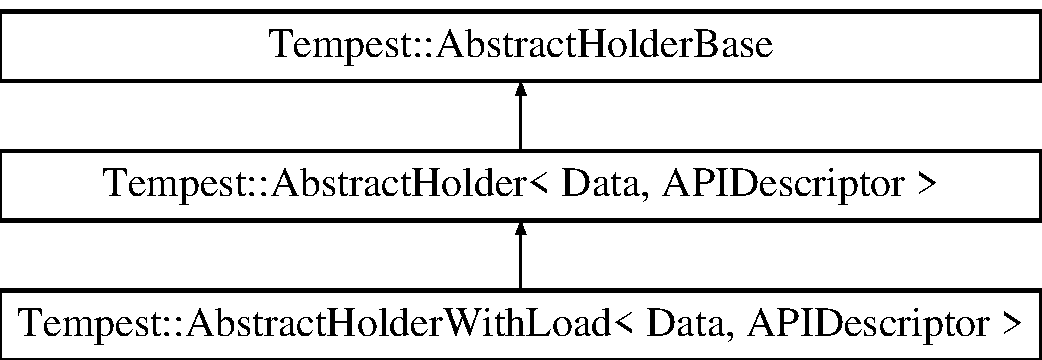
\includegraphics[height=3.000000cm]{class_tempest_1_1_abstract_holder}
\end{center}
\end{figure}
\subsection*{Classes}
\begin{DoxyCompactItemize}
\item 
struct \hyperlink{struct_tempest_1_1_abstract_holder_1_1_impl_manip}{Impl\+Manip}
\end{DoxyCompactItemize}
\subsection*{Public Member Functions}
\begin{DoxyCompactItemize}
\item 
\hypertarget{class_tempest_1_1_abstract_holder_a0b726bb7e9ca6096bc6ac65bdd67a861}{\hyperlink{struct_tempest_1_1_abstract_holder_1_1_impl_manip}{Impl\+Manip} {\bfseries make\+Manip} ()}\label{class_tempest_1_1_abstract_holder_a0b726bb7e9ca6096bc6ac65bdd67a861}

\end{DoxyCompactItemize}
\subsection*{Protected Member Functions}
\begin{DoxyCompactItemize}
\item 
\hypertarget{class_tempest_1_1_abstract_holder_a18450dd3cbbee590b7ce3bf8ab554693}{{\bfseries Abstract\+Holder} (\hyperlink{class_tempest_1_1_device}{Device} \&d)}\label{class_tempest_1_1_abstract_holder_a18450dd3cbbee590b7ce3bf8ab554693}

\item 
\hypertarget{class_tempest_1_1_abstract_holder_ac2d68f34e248226f688b4c96a479c332}{virtual void {\bfseries delete\+Object} (A\+P\+I\+Descriptor $\ast$t)=0}\label{class_tempest_1_1_abstract_holder_ac2d68f34e248226f688b4c96a479c332}

\item 
\hypertarget{class_tempest_1_1_abstract_holder_aec2c61461b9097cd6d056a7444ecbbc4}{virtual void {\bfseries reset} (A\+P\+I\+Descriptor $\ast$)=0}\label{class_tempest_1_1_abstract_holder_aec2c61461b9097cd6d056a7444ecbbc4}

\item 
\hypertarget{class_tempest_1_1_abstract_holder_a2980538d3d1969f90b03ecd97f319927}{virtual A\+P\+I\+Descriptor $\ast$ {\bfseries restore} (A\+P\+I\+Descriptor $\ast$)=0}\label{class_tempest_1_1_abstract_holder_a2980538d3d1969f90b03ecd97f319927}

\item 
\hypertarget{class_tempest_1_1_abstract_holder_ad62a1b7d1a3edbea11e08915c7326f84}{virtual A\+P\+I\+Descriptor $\ast$ {\bfseries copy} (A\+P\+I\+Descriptor $\ast$)=0}\label{class_tempest_1_1_abstract_holder_ad62a1b7d1a3edbea11e08915c7326f84}

\item 
\hypertarget{class_tempest_1_1_abstract_holder_a2a3c710af556996e79e7a3cffdd130df}{void {\bfseries reset} ()}\label{class_tempest_1_1_abstract_holder_a2a3c710af556996e79e7a3cffdd130df}

\item 
\hypertarget{class_tempest_1_1_abstract_holder_a0a2337fbe431a8e66a03cefbb32cb14f}{bool {\bfseries restore} ()}\label{class_tempest_1_1_abstract_holder_a0a2337fbe431a8e66a03cefbb32cb14f}

\end{DoxyCompactItemize}
\subsection*{Protected Attributes}
\begin{DoxyCompactItemize}
\item 
\hypertarget{class_tempest_1_1_abstract_holder_a20c1e018671da2af7514c8626bd4a9b1}{std\+::vector$<$ \hyperlink{struct_tempest_1_1_abstract_holder_1_1_impl_manip_1_1_ref}{Ref} $\ast$ $>$ {\bfseries references}}\label{class_tempest_1_1_abstract_holder_a20c1e018671da2af7514c8626bd4a9b1}

\item 
\hypertarget{class_tempest_1_1_abstract_holder_a007727dc9b2da1d226d3c88db57519d8}{\hyperlink{class_tempest_1_1_mem_pool}{Mem\+Pool}$<$ \hyperlink{struct_tempest_1_1_abstract_holder_1_1_impl_manip_1_1_ref}{Ref} $>$ {\bfseries pool}}\label{class_tempest_1_1_abstract_holder_a007727dc9b2da1d226d3c88db57519d8}

\end{DoxyCompactItemize}


The documentation for this class was generated from the following file\+:\begin{DoxyCompactItemize}
\item 
data\+Control/abstractholder.\+h\end{DoxyCompactItemize}

\hypertarget{class_tempest_1_1_abstract_holder_base}{\section{Tempest\+:\+:Abstract\+Holder\+Base Class Reference}
\label{class_tempest_1_1_abstract_holder_base}\index{Tempest\+::\+Abstract\+Holder\+Base@{Tempest\+::\+Abstract\+Holder\+Base}}
}
Inheritance diagram for Tempest\+:\+:Abstract\+Holder\+Base\+:\begin{figure}[H]
\begin{center}
\leavevmode
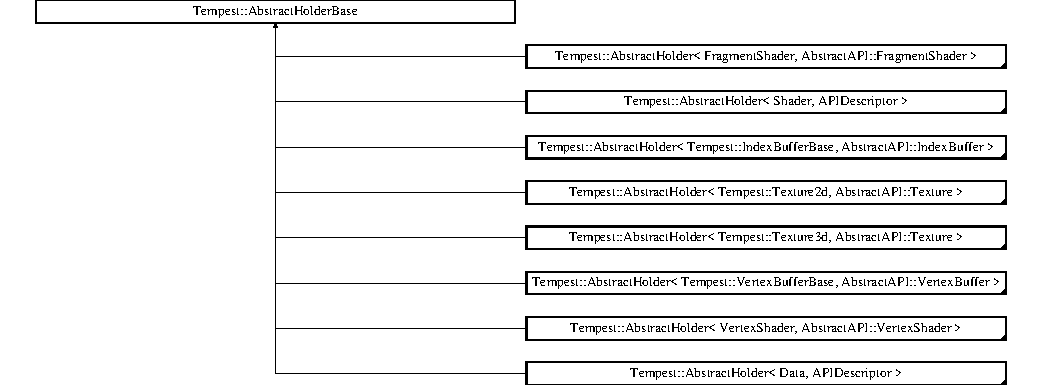
\includegraphics[height=5.174538cm]{class_tempest_1_1_abstract_holder_base}
\end{center}
\end{figure}
\subsection*{Public Member Functions}
\begin{DoxyCompactItemize}
\item 
\hypertarget{class_tempest_1_1_abstract_holder_base_aed21fc777d26c700eeedf889297371eb}{{\bfseries Abstract\+Holder\+Base} (\hyperlink{class_tempest_1_1_device}{Device} \&d)}\label{class_tempest_1_1_abstract_holder_base_aed21fc777d26c700eeedf889297371eb}

\item 
\hypertarget{class_tempest_1_1_abstract_holder_base_af9f56b2760cea7fd5fa07b88471c37b3}{\hyperlink{class_tempest_1_1_device}{Device} \& {\bfseries device} ()}\label{class_tempest_1_1_abstract_holder_base_af9f56b2760cea7fd5fa07b88471c37b3}

\item 
\hypertarget{class_tempest_1_1_abstract_holder_base_af2469a93aed33f7cf0108e0dc92932f1}{\hyperlink{class_tempest_1_1_device}{Device} \& {\bfseries device} () const }\label{class_tempest_1_1_abstract_holder_base_af2469a93aed33f7cf0108e0dc92932f1}

\end{DoxyCompactItemize}
\subsection*{Protected Member Functions}
\begin{DoxyCompactItemize}
\item 
\hypertarget{class_tempest_1_1_abstract_holder_base_a1293a281f8e570a363cd40f2a8e2c226}{virtual void {\bfseries reset} ()=0}\label{class_tempest_1_1_abstract_holder_base_a1293a281f8e570a363cd40f2a8e2c226}

\item 
\hypertarget{class_tempest_1_1_abstract_holder_base_a7a02232061d5d98ae1760482dfb8e031}{virtual bool {\bfseries restore} ()=0}\label{class_tempest_1_1_abstract_holder_base_a7a02232061d5d98ae1760482dfb8e031}

\item 
\hypertarget{class_tempest_1_1_abstract_holder_base_ac50ce07eb80c2d47a0704becd0e99fbd}{virtual void {\bfseries present\+Event} ()}\label{class_tempest_1_1_abstract_holder_base_ac50ce07eb80c2d47a0704becd0e99fbd}

\end{DoxyCompactItemize}
\subsection*{Protected Attributes}
\begin{DoxyCompactItemize}
\item 
\hypertarget{class_tempest_1_1_abstract_holder_base_a6a8cc8e516aee275a4d14a08c955eb70}{\hyperlink{class_tempest_1_1_device}{Device} \& {\bfseries m\+\_\+device}}\label{class_tempest_1_1_abstract_holder_base_a6a8cc8e516aee275a4d14a08c955eb70}

\end{DoxyCompactItemize}
\subsection*{Friends}
\begin{DoxyCompactItemize}
\item 
\hypertarget{class_tempest_1_1_abstract_holder_base_a520fa05e0bf58785da428f7a0241eee2}{class {\bfseries Device}}\label{class_tempest_1_1_abstract_holder_base_a520fa05e0bf58785da428f7a0241eee2}

\end{DoxyCompactItemize}


The documentation for this class was generated from the following files\+:\begin{DoxyCompactItemize}
\item 
data\+Control/abstractholder.\+h\item 
data\+Control/abstractholder.\+cpp\end{DoxyCompactItemize}

\hypertarget{class_tempest_1_1_abstract_holder_with_load}{\section{Tempest\+:\+:Abstract\+Holder\+With\+Load$<$ Data, A\+P\+I\+Descriptor $>$ Class Template Reference}
\label{class_tempest_1_1_abstract_holder_with_load}\index{Tempest\+::\+Abstract\+Holder\+With\+Load$<$ Data, A\+P\+I\+Descriptor $>$@{Tempest\+::\+Abstract\+Holder\+With\+Load$<$ Data, A\+P\+I\+Descriptor $>$}}
}
Inheritance diagram for Tempest\+:\+:Abstract\+Holder\+With\+Load$<$ Data, A\+P\+I\+Descriptor $>$\+:\begin{figure}[H]
\begin{center}
\leavevmode
\includegraphics[height=3.000000cm]{class_tempest_1_1_abstract_holder_with_load}
\end{center}
\end{figure}
\subsection*{Public Types}
\begin{DoxyCompactItemize}
\item 
\hypertarget{class_tempest_1_1_abstract_holder_with_load_aab5a7dc94f9cdf1c8b1b2c9c4de1b116}{typedef \hyperlink{class_tempest_1_1_abstract_holder}{Abstract\+Holder}$<$ Data, \\*
A\+P\+I\+Descriptor $>$\+::\hyperlink{struct_tempest_1_1_abstract_holder_1_1_impl_manip}{Impl\+Manip} {\bfseries Impl\+Manip}}\label{class_tempest_1_1_abstract_holder_with_load_aab5a7dc94f9cdf1c8b1b2c9c4de1b116}

\end{DoxyCompactItemize}
\subsection*{Public Member Functions}
\begin{DoxyCompactItemize}
\item 
\hypertarget{class_tempest_1_1_abstract_holder_with_load_a90f46d815e2a53ff0d3600953188f4e0}{{\bfseries Abstract\+Holder\+With\+Load} (\hyperlink{class_tempest_1_1_device}{Device} \&d)}\label{class_tempest_1_1_abstract_holder_with_load_a90f46d815e2a53ff0d3600953188f4e0}

\item 
\hypertarget{class_tempest_1_1_abstract_holder_with_load_a3bd2b216d74bc441d3be1fddad623a51}{virtual Data {\bfseries load} (\hyperlink{class_tempest_1_1_i_device}{I\+Device} \&file)}\label{class_tempest_1_1_abstract_holder_with_load_a3bd2b216d74bc441d3be1fddad623a51}

\item 
\hypertarget{class_tempest_1_1_abstract_holder_with_load_a66e464edaae4396b0329433cc8bb0da0}{virtual Data {\bfseries load} (const std\+::u16string \&fname)}\label{class_tempest_1_1_abstract_holder_with_load_a66e464edaae4396b0329433cc8bb0da0}

\item 
\hypertarget{class_tempest_1_1_abstract_holder_with_load_a9cffce4ee46bafb0c7ec4c0e878bd60e}{virtual Data {\bfseries load} (const std\+::string \&fname)}\label{class_tempest_1_1_abstract_holder_with_load_a9cffce4ee46bafb0c7ec4c0e878bd60e}

\item 
\hypertarget{class_tempest_1_1_abstract_holder_with_load_a88692e896206253de9012bafbb18fc0a}{virtual Data {\bfseries load} (const char $\ast$fname)}\label{class_tempest_1_1_abstract_holder_with_load_a88692e896206253de9012bafbb18fc0a}

\end{DoxyCompactItemize}
\subsection*{Protected Member Functions}
\begin{DoxyCompactItemize}
\item 
\hypertarget{class_tempest_1_1_abstract_holder_with_load_aa3241b750aea46fee5c05c83aad62833}{virtual void {\bfseries create\+Object} (Data \&, A\+P\+I\+Descriptor $\ast$\&t, const std\+::string \&fname)}\label{class_tempest_1_1_abstract_holder_with_load_aa3241b750aea46fee5c05c83aad62833}

\item 
\hypertarget{class_tempest_1_1_abstract_holder_with_load_a366d654c361bd8618ba7f9a07efbcb08}{virtual void {\bfseries create\+Object} (Data \&, A\+P\+I\+Descriptor $\ast$\&t, const std\+::u16string \&fname)}\label{class_tempest_1_1_abstract_holder_with_load_a366d654c361bd8618ba7f9a07efbcb08}

\item 
\hypertarget{class_tempest_1_1_abstract_holder_with_load_a57bbc7ddd024c9669c054058774e00b4}{virtual void {\bfseries create\+Object} (Data \&, A\+P\+I\+Descriptor $\ast$\&t, \hyperlink{class_tempest_1_1_i_device}{I\+Device} \&file)}\label{class_tempest_1_1_abstract_holder_with_load_a57bbc7ddd024c9669c054058774e00b4}

\item 
\hypertarget{class_tempest_1_1_abstract_holder_with_load_ae8fc90320d0beba4724e111c3d9715ac}{virtual void {\bfseries create\+Object} (A\+P\+I\+Descriptor $\ast$\&t, const std\+::string \&fname)}\label{class_tempest_1_1_abstract_holder_with_load_ae8fc90320d0beba4724e111c3d9715ac}

\item 
\hypertarget{class_tempest_1_1_abstract_holder_with_load_a6e924e57b4089d480b35e69920851ccb}{virtual void {\bfseries create\+Object} (A\+P\+I\+Descriptor $\ast$\&t, const std\+::u16string \&fname)}\label{class_tempest_1_1_abstract_holder_with_load_a6e924e57b4089d480b35e69920851ccb}

\item 
\hypertarget{class_tempest_1_1_abstract_holder_with_load_a70a851d9ca7d2598e2c1658190772b12}{virtual void {\bfseries create\+Object} (A\+P\+I\+Descriptor $\ast$\&t, \hyperlink{class_tempest_1_1_i_device}{I\+Device} \&file)=0}\label{class_tempest_1_1_abstract_holder_with_load_a70a851d9ca7d2598e2c1658190772b12}

\end{DoxyCompactItemize}
\subsection*{Additional Inherited Members}


The documentation for this class was generated from the following file\+:\begin{DoxyCompactItemize}
\item 
data\+Control/abstractholder.\+h\end{DoxyCompactItemize}

\hypertarget{class_tempest_1_1_abstract_i_o_device}{\section{Tempest\+:\+:Abstract\+I\+O\+Device Class Reference}
\label{class_tempest_1_1_abstract_i_o_device}\index{Tempest\+::\+Abstract\+I\+O\+Device@{Tempest\+::\+Abstract\+I\+O\+Device}}
}
Inheritance diagram for Tempest\+:\+:Abstract\+I\+O\+Device\+:\begin{figure}[H]
\begin{center}
\leavevmode
\includegraphics[height=1.395349cm]{class_tempest_1_1_abstract_i_o_device}
\end{center}
\end{figure}


The documentation for this class was generated from the following file\+:\begin{DoxyCompactItemize}
\item 
io/iodevice.\+h\end{DoxyCompactItemize}

\hypertarget{class_tempest_1_1_abstract_light_collection}{\section{Tempest\+:\+:Abstract\+Light\+Collection Class Reference}
\label{class_tempest_1_1_abstract_light_collection}\index{Tempest\+::\+Abstract\+Light\+Collection@{Tempest\+::\+Abstract\+Light\+Collection}}
}
Inheritance diagram for Tempest\+:\+:Abstract\+Light\+Collection\+:\begin{figure}[H]
\begin{center}
\leavevmode
\includegraphics[height=2.000000cm]{class_tempest_1_1_abstract_light_collection}
\end{center}
\end{figure}
\subsection*{Classes}
\begin{DoxyCompactItemize}
\item 
class \hyperlink{class_tempest_1_1_abstract_light_collection_1_1_pack}{Pack}
\end{DoxyCompactItemize}
\subsection*{Public Types}
\begin{DoxyCompactItemize}
\item 
\hypertarget{class_tempest_1_1_abstract_light_collection_a2291e4a1d1006cb1d05069e09166a50e}{typedef \hyperlink{class_tempest_1_1_abstract_light_collection_1_1_pack}{Pack}$<$ \hyperlink{class_tempest_1_1_direction_light}{Direction\+Light} $>$ {\bfseries Direction\+Lights}}\label{class_tempest_1_1_abstract_light_collection_a2291e4a1d1006cb1d05069e09166a50e}

\end{DoxyCompactItemize}
\subsection*{Public Member Functions}
\begin{DoxyCompactItemize}
\item 
\hypertarget{class_tempest_1_1_abstract_light_collection_a92168e9e668f1ab4b8c5b41a2fb28a95}{virtual const \hyperlink{class_tempest_1_1_abstract_light_collection_1_1_pack}{Direction\+Lights} \& {\bfseries direction} () const =0}\label{class_tempest_1_1_abstract_light_collection_a92168e9e668f1ab4b8c5b41a2fb28a95}

\item 
\hypertarget{class_tempest_1_1_abstract_light_collection_ae327ede02c4371f165db9a61117ee260}{virtual \hyperlink{class_tempest_1_1_abstract_light_collection_1_1_pack}{Direction\+Lights} \& {\bfseries direction} ()=0}\label{class_tempest_1_1_abstract_light_collection_ae327ede02c4371f165db9a61117ee260}

\end{DoxyCompactItemize}


The documentation for this class was generated from the following file\+:\begin{DoxyCompactItemize}
\item 
scene/abstractlightcollection.\+h\end{DoxyCompactItemize}

\hypertarget{class_tempest_1_1_abstract_scene}{\section{Tempest\+:\+:Abstract\+Scene$<$ Item $>$ Class Template Reference}
\label{class_tempest_1_1_abstract_scene}\index{Tempest\+::\+Abstract\+Scene$<$ Item $>$@{Tempest\+::\+Abstract\+Scene$<$ Item $>$}}
}
\subsection*{Public Member Functions}
\begin{DoxyCompactItemize}
\item 
\hypertarget{class_tempest_1_1_abstract_scene_aca4d534e1e081093f50dfc0e7474dc67}{{\footnotesize template$<$class V $>$ }\\void {\bfseries set\+View\+Tester} (const V \&c)}\label{class_tempest_1_1_abstract_scene_aca4d534e1e081093f50dfc0e7474dc67}

\item 
\hypertarget{class_tempest_1_1_abstract_scene_a834440cb1ae408c16c42c4099534cc51}{const \hyperlink{class_tempest_1_1_view_tester}{View\+Tester} \& {\bfseries view\+Tester} () const }\label{class_tempest_1_1_abstract_scene_a834440cb1ae408c16c42c4099534cc51}

\item 
\hypertarget{class_tempest_1_1_abstract_scene_ac7c5496c586b0b4f611e9a554a436410}{{\footnotesize template$<$class C $>$ }\\void {\bfseries set\+Camera} (const C \&c)}\label{class_tempest_1_1_abstract_scene_ac7c5496c586b0b4f611e9a554a436410}

\item 
\hypertarget{class_tempest_1_1_abstract_scene_a431c2b26d9ec11097a2b523784908db8}{const \hyperlink{class_tempest_1_1_abstract_camera}{Abstract\+Camera} \& {\bfseries camera} () const }\label{class_tempest_1_1_abstract_scene_a431c2b26d9ec11097a2b523784908db8}

\item 
\hypertarget{class_tempest_1_1_abstract_scene_a46a27924de77f46a44506472ce372426}{{\footnotesize template$<$class L $>$ }\\void {\bfseries set\+Light\+Collection} (const L \&l)}\label{class_tempest_1_1_abstract_scene_a46a27924de77f46a44506472ce372426}

\item 
\hypertarget{class_tempest_1_1_abstract_scene_a5d7c32ca63959fa02cf2ef806725c2e8}{const \hyperlink{class_tempest_1_1_abstract_light_collection}{Abstract\+Light\+Collection} \& {\bfseries lights} () const }\label{class_tempest_1_1_abstract_scene_a5d7c32ca63959fa02cf2ef806725c2e8}

\item 
\hypertarget{class_tempest_1_1_abstract_scene_adaf166ff86831c58adccf2d2cdb53da2}{\hyperlink{class_tempest_1_1_abstract_light_collection}{Abstract\+Light\+Collection} \& {\bfseries lights} ()}\label{class_tempest_1_1_abstract_scene_adaf166ff86831c58adccf2d2cdb53da2}

\end{DoxyCompactItemize}
\subsection*{Protected Member Functions}
\begin{DoxyCompactItemize}
\item 
\hypertarget{class_tempest_1_1_abstract_scene_a884fe6c22b0411cd2524ad56c479ab25}{virtual void {\bfseries on\+Object\+Added} (const Item $\ast$)}\label{class_tempest_1_1_abstract_scene_a884fe6c22b0411cd2524ad56c479ab25}

\item 
\hypertarget{class_tempest_1_1_abstract_scene_abf238d953a486566d561a8d7a6d89923}{virtual void {\bfseries on\+Object\+Removed} (const Item $\ast$)}\label{class_tempest_1_1_abstract_scene_abf238d953a486566d561a8d7a6d89923}

\item 
\hypertarget{class_tempest_1_1_abstract_scene_ad2628ef9b9b8c74da2d2353f30e900d5}{virtual void {\bfseries on\+Object\+Transform} (const Item $\ast$, const \hyperlink{class_tempest_1_1_matrix4x4}{Tempest\+::\+Matrix4x4} \&)}\label{class_tempest_1_1_abstract_scene_ad2628ef9b9b8c74da2d2353f30e900d5}

\end{DoxyCompactItemize}
\subsection*{Friends}
\begin{DoxyCompactItemize}
\item 
\hypertarget{class_tempest_1_1_abstract_scene_a3462d35d40dbded673b4160d2a4f9dc6}{{\footnotesize template$<$class M $>$ }\\class {\bfseries Tempest\+::\+Abstract\+Graphic\+Object}}\label{class_tempest_1_1_abstract_scene_a3462d35d40dbded673b4160d2a4f9dc6}

\end{DoxyCompactItemize}


The documentation for this class was generated from the following file\+:\begin{DoxyCompactItemize}
\item 
scene/abstractscene.\+h\end{DoxyCompactItemize}

\hypertarget{class_tempest_1_1_abstract_scene_object}{\section{Tempest\+:\+:Abstract\+Scene\+Object Class Reference}
\label{class_tempest_1_1_abstract_scene_object}\index{Tempest\+::\+Abstract\+Scene\+Object@{Tempest\+::\+Abstract\+Scene\+Object}}
}
Inheritance diagram for Tempest\+:\+:Abstract\+Scene\+Object\+:\begin{figure}[H]
\begin{center}
\leavevmode
\includegraphics[height=3.000000cm]{class_tempest_1_1_abstract_scene_object}
\end{center}
\end{figure}
\subsection*{Public Member Functions}
\begin{DoxyCompactItemize}
\item 
\hypertarget{class_tempest_1_1_abstract_scene_object_accb054d8782d5a95b4e0f226bb1764ab}{{\bfseries Abstract\+Scene\+Object} (const \hyperlink{class_tempest_1_1_abstract_scene_object}{Abstract\+Scene\+Object} \&obj)}\label{class_tempest_1_1_abstract_scene_object_accb054d8782d5a95b4e0f226bb1764ab}

\item 
\hypertarget{class_tempest_1_1_abstract_scene_object_a8fedce6cff933e8e6a30d75e9aeba21b}{\hyperlink{class_tempest_1_1_abstract_scene_object}{Abstract\+Scene\+Object} \& {\bfseries operator=} (const \hyperlink{class_tempest_1_1_abstract_scene_object}{Abstract\+Scene\+Object} \&obj)}\label{class_tempest_1_1_abstract_scene_object_a8fedce6cff933e8e6a30d75e9aeba21b}

\item 
\hypertarget{class_tempest_1_1_abstract_scene_object_a0bbfe890cd7669613461f7ecccbf8e16}{virtual const \hyperlink{struct_tempest_1_1_model_bounds}{Model\+Bounds} \& {\bfseries bounds} () const =0}\label{class_tempest_1_1_abstract_scene_object_a0bbfe890cd7669613461f7ecccbf8e16}

\item 
\hypertarget{class_tempest_1_1_abstract_scene_object_a5a73eb01bcf835bb1b3fc674cea393f2}{virtual const \hyperlink{class_tempest_1_1_matrix4x4}{Matrix4x4} \& {\bfseries transform} () const =0}\label{class_tempest_1_1_abstract_scene_object_a5a73eb01bcf835bb1b3fc674cea393f2}

\item 
\hypertarget{class_tempest_1_1_abstract_scene_object_af9ed012dd9e5ffabb91bc677240eca96}{bool {\bfseries is\+Visible} () const }\label{class_tempest_1_1_abstract_scene_object_af9ed012dd9e5ffabb91bc677240eca96}

\item 
\hypertarget{class_tempest_1_1_abstract_scene_object_a0c442c68760482b77be088ff26f20ec1}{void {\bfseries set\+Visible} (bool v)}\label{class_tempest_1_1_abstract_scene_object_a0c442c68760482b77be088ff26f20ec1}

\item 
\hypertarget{class_tempest_1_1_abstract_scene_object_ad3257a9d87ac338a0d4b5ce66aba56a3}{virtual float {\bfseries x} () const =0}\label{class_tempest_1_1_abstract_scene_object_ad3257a9d87ac338a0d4b5ce66aba56a3}

\item 
\hypertarget{class_tempest_1_1_abstract_scene_object_a875dae888de29b0aa9387dd1e8b684eb}{virtual float {\bfseries y} () const =0}\label{class_tempest_1_1_abstract_scene_object_a875dae888de29b0aa9387dd1e8b684eb}

\item 
\hypertarget{class_tempest_1_1_abstract_scene_object_a0c9048cdd609083f54ad8b7f03b90021}{virtual float {\bfseries z} () const =0}\label{class_tempest_1_1_abstract_scene_object_a0c9048cdd609083f54ad8b7f03b90021}

\item 
\hypertarget{class_tempest_1_1_abstract_scene_object_af73349b4acb4c9fad3abe3e337402343}{virtual float {\bfseries size\+X} () const =0}\label{class_tempest_1_1_abstract_scene_object_af73349b4acb4c9fad3abe3e337402343}

\item 
\hypertarget{class_tempest_1_1_abstract_scene_object_af0c7c366e0d160159e0ffc7ca165c70f}{virtual float {\bfseries size\+Y} () const =0}\label{class_tempest_1_1_abstract_scene_object_af0c7c366e0d160159e0ffc7ca165c70f}

\item 
\hypertarget{class_tempest_1_1_abstract_scene_object_add83241e8f4cc9a51c2e9f0ebb3ac4cd}{virtual float {\bfseries size\+Z} () const =0}\label{class_tempest_1_1_abstract_scene_object_add83241e8f4cc9a51c2e9f0ebb3ac4cd}

\item 
\hypertarget{class_tempest_1_1_abstract_scene_object_a2fb08be9fae7ef8c5d422b9c47650a16}{virtual float {\bfseries radius} () const =0}\label{class_tempest_1_1_abstract_scene_object_a2fb08be9fae7ef8c5d422b9c47650a16}

\end{DoxyCompactItemize}
\subsection*{Protected Member Functions}
\begin{DoxyCompactItemize}
\item 
\hypertarget{class_tempest_1_1_abstract_scene_object_adeafe373523ba8a6d2f490977e808b50}{virtual void {\bfseries on\+Transform\+Changed} (const \hyperlink{class_tempest_1_1_matrix4x4}{Tempest\+::\+Matrix4x4} \&old) const =0}\label{class_tempest_1_1_abstract_scene_object_adeafe373523ba8a6d2f490977e808b50}

\end{DoxyCompactItemize}
\subsection*{Friends}
\begin{DoxyCompactItemize}
\item 
\hypertarget{class_tempest_1_1_abstract_scene_object_a032858ae1fe02d2d1170981c2af2d67c}{class {\bfseries Scene}}\label{class_tempest_1_1_abstract_scene_object_a032858ae1fe02d2d1170981c2af2d67c}

\item 
\hypertarget{class_tempest_1_1_abstract_scene_object_ad962652a5ca57a062e87b84d43dad6a3}{class {\bfseries Render}}\label{class_tempest_1_1_abstract_scene_object_ad962652a5ca57a062e87b84d43dad6a3}

\end{DoxyCompactItemize}


The documentation for this class was generated from the following file\+:\begin{DoxyCompactItemize}
\item 
scene/abstractgraphicobject.\+h\end{DoxyCompactItemize}

\hypertarget{class_tempest_1_1_abstract_shading_lang}{\section{Tempest\+:\+:Abstract\+Shading\+Lang Class Reference}
\label{class_tempest_1_1_abstract_shading_lang}\index{Tempest\+::\+Abstract\+Shading\+Lang@{Tempest\+::\+Abstract\+Shading\+Lang}}
}
Inheritance diagram for Tempest\+:\+:Abstract\+Shading\+Lang\+:\begin{figure}[H]
\begin{center}
\leavevmode
\includegraphics[height=2.901554cm]{class_tempest_1_1_abstract_shading_lang}
\end{center}
\end{figure}
\subsection*{Classes}
\begin{DoxyCompactItemize}
\item 
struct \hyperlink{struct_tempest_1_1_abstract_shading_lang_1_1_ui_shader_opt}{Ui\+Shader\+Opt}
\end{DoxyCompactItemize}
\subsection*{Public Member Functions}
\begin{DoxyCompactItemize}
\item 
\hypertarget{class_tempest_1_1_abstract_shading_lang_a9eff85626d4959dcd3f4d7aeae26afb9}{{\bfseries Abstract\+Shading\+Lang} (const \hyperlink{class_tempest_1_1_abstract_shading_lang}{Abstract\+Shading\+Lang} \&)=delete}\label{class_tempest_1_1_abstract_shading_lang_a9eff85626d4959dcd3f4d7aeae26afb9}

\item 
\hypertarget{class_tempest_1_1_abstract_shading_lang_a2b34979e7d5e71ecb62f794c24193250}{\hyperlink{class_tempest_1_1_abstract_shading_lang}{Abstract\+Shading\+Lang} \& {\bfseries operator=} (const \hyperlink{class_tempest_1_1_abstract_shading_lang}{Abstract\+Shading\+Lang} \&)=delete}\label{class_tempest_1_1_abstract_shading_lang_a2b34979e7d5e71ecb62f794c24193250}

\item 
\hypertarget{class_tempest_1_1_abstract_shading_lang_ae99c7ea6c48f482580a4c03c0b2f6003}{virtual void {\bfseries begin\+Paint} () const }\label{class_tempest_1_1_abstract_shading_lang_ae99c7ea6c48f482580a4c03c0b2f6003}

\item 
\hypertarget{class_tempest_1_1_abstract_shading_lang_a378c2e82c7e2a6b50fee2c2becb3b7e7}{virtual void {\bfseries end\+Paint} () const }\label{class_tempest_1_1_abstract_shading_lang_a378c2e82c7e2a6b50fee2c2becb3b7e7}

\item 
\hypertarget{class_tempest_1_1_abstract_shading_lang_a6441662806c2437e55687252daec74e0}{virtual void {\bfseries enable} () const }\label{class_tempest_1_1_abstract_shading_lang_a6441662806c2437e55687252daec74e0}

\item 
\hypertarget{class_tempest_1_1_abstract_shading_lang_a8fd78424270fa6f9ed5829db477666fd}{virtual void {\bfseries disable} () const }\label{class_tempest_1_1_abstract_shading_lang_a8fd78424270fa6f9ed5829db477666fd}

\item 
\hypertarget{class_tempest_1_1_abstract_shading_lang_a858e44675836052523af3a988b52ddc2}{virtual void {\bfseries bind} (const \hyperlink{class_tempest_1_1_vertex_shader}{Tempest\+::\+Vertex\+Shader} \&) const =0}\label{class_tempest_1_1_abstract_shading_lang_a858e44675836052523af3a988b52ddc2}

\item 
\hypertarget{class_tempest_1_1_abstract_shading_lang_accc0e1d115d2be9b627115e394c124c5}{virtual void {\bfseries bind} (const \hyperlink{class_tempest_1_1_fragment_shader}{Tempest\+::\+Fragment\+Shader} \&) const =0}\label{class_tempest_1_1_abstract_shading_lang_accc0e1d115d2be9b627115e394c124c5}

\item 
\hypertarget{class_tempest_1_1_abstract_shading_lang_a9b79bf98a809156da16fa6ad99fddc25}{virtual void {\bfseries un\+Bind} (const \hyperlink{class_tempest_1_1_vertex_shader}{Tempest\+::\+Vertex\+Shader} \&) const =0}\label{class_tempest_1_1_abstract_shading_lang_a9b79bf98a809156da16fa6ad99fddc25}

\item 
\hypertarget{class_tempest_1_1_abstract_shading_lang_a143ac0075977399a8613974446fcefe8}{virtual void {\bfseries un\+Bind} (const \hyperlink{class_tempest_1_1_fragment_shader}{Tempest\+::\+Fragment\+Shader} \&) const =0}\label{class_tempest_1_1_abstract_shading_lang_a143ac0075977399a8613974446fcefe8}

\item 
\hypertarget{class_tempest_1_1_abstract_shading_lang_a58477d41043ece8bab348cb84b986ab2}{virtual void {\bfseries set\+Vertex\+Decl} (const Tempest\+::\+Abstract\+A\+P\+I\+::\+Vertex\+Decl $\ast$) const }\label{class_tempest_1_1_abstract_shading_lang_a58477d41043ece8bab348cb84b986ab2}

\item 
\hypertarget{class_tempest_1_1_abstract_shading_lang_a9ee31674de9ef0299e1ebd8d229b5132}{virtual void $\ast$ {\bfseries context} () const =0}\label{class_tempest_1_1_abstract_shading_lang_a9ee31674de9ef0299e1ebd8d229b5132}

\item 
\hypertarget{class_tempest_1_1_abstract_shading_lang_aaa3bd33dacb694063d0fcade2f9ee1d3}{virtual void $\ast$ {\bfseries create\+Shader} (Shader\+Type t, const std\+::string \&fname, std\+::string \&output\+Log) const }\label{class_tempest_1_1_abstract_shading_lang_aaa3bd33dacb694063d0fcade2f9ee1d3}

\item 
\hypertarget{class_tempest_1_1_abstract_shading_lang_af7189d53ab32d39e6276ee108ba7dd82}{virtual void $\ast$ {\bfseries create\+Shader} (Shader\+Type t, const std\+::u16string \&fname, std\+::string \&output\+Log) const }\label{class_tempest_1_1_abstract_shading_lang_af7189d53ab32d39e6276ee108ba7dd82}

\item 
\hypertarget{class_tempest_1_1_abstract_shading_lang_a6863e67dadd5b78df8641d4511f972de}{virtual void $\ast$ {\bfseries create\+Shader\+From\+Source} (Shader\+Type t, const std\+::string \&src, std\+::string \&output\+Log) const }\label{class_tempest_1_1_abstract_shading_lang_a6863e67dadd5b78df8641d4511f972de}

\item 
\hypertarget{class_tempest_1_1_abstract_shading_lang_a0a21d691048dab1129878aa41a7cb575}{virtual \hyperlink{class_tempest_1_1_vertex_shader}{Vertex\+Shader} $\ast$ {\bfseries create\+Vertex\+Shader} (const std\+::string \&fname, std\+::string \&output\+Log) const }\label{class_tempest_1_1_abstract_shading_lang_a0a21d691048dab1129878aa41a7cb575}

\item 
\hypertarget{class_tempest_1_1_abstract_shading_lang_a34cf928a239bd3f8c07f83fb8e41c83e}{virtual \hyperlink{class_tempest_1_1_vertex_shader}{Vertex\+Shader} $\ast$ {\bfseries create\+Vertex\+Shader} (const std\+::u16string \&fname, std\+::string \&output\+Log) const }\label{class_tempest_1_1_abstract_shading_lang_a34cf928a239bd3f8c07f83fb8e41c83e}

\item 
\hypertarget{class_tempest_1_1_abstract_shading_lang_a169752a9b00ee3e7686ff55b82485994}{virtual \hyperlink{class_tempest_1_1_vertex_shader}{Vertex\+Shader} $\ast$ {\bfseries create\+Vertex\+Shader\+From\+Source} (const std\+::string \&src, std\+::string \&output\+Log) const =0}\label{class_tempest_1_1_abstract_shading_lang_a169752a9b00ee3e7686ff55b82485994}

\item 
\hypertarget{class_tempest_1_1_abstract_shading_lang_a7739c3d706a6c0a44a693f928a352ce6}{virtual \hyperlink{class_tempest_1_1_fragment_shader}{Fragment\+Shader} $\ast$ {\bfseries create\+Fragment\+Shader} (const std\+::string \&fname, std\+::string \&output\+Log) const }\label{class_tempest_1_1_abstract_shading_lang_a7739c3d706a6c0a44a693f928a352ce6}

\item 
\hypertarget{class_tempest_1_1_abstract_shading_lang_a9ef79d9a353842e86389adcc5ebf59e9}{virtual \hyperlink{class_tempest_1_1_fragment_shader}{Fragment\+Shader} $\ast$ {\bfseries create\+Fragment\+Shader} (const std\+::u16string \&fname, std\+::string \&log) const }\label{class_tempest_1_1_abstract_shading_lang_a9ef79d9a353842e86389adcc5ebf59e9}

\item 
\hypertarget{class_tempest_1_1_abstract_shading_lang_a6231073ccc9a432d91fbc3707c890c7c}{virtual \hyperlink{class_tempest_1_1_fragment_shader}{Fragment\+Shader} $\ast$ {\bfseries create\+Fragment\+Shader\+From\+Source} (const std\+::string \&src, std\+::string \&output\+Log) const =0}\label{class_tempest_1_1_abstract_shading_lang_a6231073ccc9a432d91fbc3707c890c7c}

\item 
\hypertarget{class_tempest_1_1_abstract_shading_lang_abf1319678d3154fa8d5161060da0d82a}{void {\bfseries delete\+Shader} (\hyperlink{class_tempest_1_1_vertex_shader}{Vertex\+Shader} $\ast$s) const }\label{class_tempest_1_1_abstract_shading_lang_abf1319678d3154fa8d5161060da0d82a}

\item 
\hypertarget{class_tempest_1_1_abstract_shading_lang_ab56e87f58cce30a4c251a238cfe785df}{void {\bfseries delete\+Shader} (\hyperlink{class_tempest_1_1_fragment_shader}{Fragment\+Shader} $\ast$s) const }\label{class_tempest_1_1_abstract_shading_lang_ab56e87f58cce30a4c251a238cfe785df}

\item 
\hypertarget{class_tempest_1_1_abstract_shading_lang_aa18f3296adbd9353b5d7a775d53df0a7}{virtual void {\bfseries delete\+Vertex\+Shader} (\hyperlink{class_tempest_1_1_vertex_shader}{Vertex\+Shader} $\ast$s) const =0}\label{class_tempest_1_1_abstract_shading_lang_aa18f3296adbd9353b5d7a775d53df0a7}

\item 
\hypertarget{class_tempest_1_1_abstract_shading_lang_aeab500f02550a17655ebb1206a047751}{virtual void {\bfseries delete\+Fragment\+Shader} (\hyperlink{class_tempest_1_1_fragment_shader}{Fragment\+Shader} $\ast$s) const =0}\label{class_tempest_1_1_abstract_shading_lang_aeab500f02550a17655ebb1206a047751}

\item 
\hypertarget{class_tempest_1_1_abstract_shading_lang_ae1b8d4e6da76a246775abe341893d152}{virtual bool {\bfseries link} (const \hyperlink{class_tempest_1_1_vertex_shader}{Tempest\+::\+Vertex\+Shader} \&, const \hyperlink{class_tempest_1_1_fragment_shader}{Tempest\+::\+Fragment\+Shader} \&, const Abstract\+A\+P\+I\+::\+Vertex\+Decl $\ast$, std\+::string \&) const }\label{class_tempest_1_1_abstract_shading_lang_ae1b8d4e6da76a246775abe341893d152}

\item 
\hypertarget{class_tempest_1_1_abstract_shading_lang_aebb129c683a45c1ef61389b2a27e145a}{virtual std\+::string {\bfseries surface\+Shader} (Shader\+Type t, const \hyperlink{struct_tempest_1_1_abstract_shading_lang_1_1_ui_shader_opt}{Ui\+Shader\+Opt} \&, bool \&has\+Halfpix\+Offset) const =0}\label{class_tempest_1_1_abstract_shading_lang_aebb129c683a45c1ef61389b2a27e145a}

\item 
\hypertarget{class_tempest_1_1_abstract_shading_lang_afaea6209707e1c39c8be5b80827e1db3}{virtual std\+::string {\bfseries surface\+Shader} (Shader\+Type t, const \hyperlink{struct_tempest_1_1_abstract_shading_lang_1_1_ui_shader_opt}{Ui\+Shader\+Opt} \&opt) const }\label{class_tempest_1_1_abstract_shading_lang_afaea6209707e1c39c8be5b80827e1db3}

\end{DoxyCompactItemize}
\subsection*{Static Protected Member Functions}
\begin{DoxyCompactItemize}
\item 
\hypertarget{class_tempest_1_1_abstract_shading_lang_a863f677f069eb0cfed38e66dd1127af0}{static \hyperlink{class_tempest_1_1_vertex_shader}{Vertex\+Shader} $\ast$ {\bfseries get} (const \hyperlink{class_tempest_1_1_vertex_shader}{Tempest\+::\+Vertex\+Shader} \&s)}\label{class_tempest_1_1_abstract_shading_lang_a863f677f069eb0cfed38e66dd1127af0}

\item 
\hypertarget{class_tempest_1_1_abstract_shading_lang_a7bc232ad8cb628968aab014b3db73dd7}{static \hyperlink{class_tempest_1_1_fragment_shader}{Fragment\+Shader} $\ast$ {\bfseries get} (const \hyperlink{class_tempest_1_1_fragment_shader}{Tempest\+::\+Fragment\+Shader} \&s)}\label{class_tempest_1_1_abstract_shading_lang_a7bc232ad8cb628968aab014b3db73dd7}

\item 
\hypertarget{class_tempest_1_1_abstract_shading_lang_af1c414ce2e4027b35ff7003170340437}{static Abstract\+A\+P\+I\+::\+Texture $\ast$ {\bfseries get} (const \hyperlink{class_tempest_1_1_texture2d}{Tempest\+::\+Texture2d} \&s)}\label{class_tempest_1_1_abstract_shading_lang_af1c414ce2e4027b35ff7003170340437}

\item 
\hypertarget{class_tempest_1_1_abstract_shading_lang_ab499ab8fa4032e48fee12c90665ae85f}{static Abstract\+A\+P\+I\+::\+Texture $\ast$ {\bfseries get} (const \hyperlink{class_tempest_1_1_texture3d}{Tempest\+::\+Texture3d} \&s)}\label{class_tempest_1_1_abstract_shading_lang_ab499ab8fa4032e48fee12c90665ae85f}

\item 
\hypertarget{class_tempest_1_1_abstract_shading_lang_ab7d8a834f90091ca36fe7beae9ade0ca}{static const \hyperlink{class_tempest_1_1_shader_input}{Shader\+Input} \& {\bfseries input\+Of} (const \hyperlink{class_tempest_1_1_vertex_shader}{Tempest\+::\+Vertex\+Shader} \&s)}\label{class_tempest_1_1_abstract_shading_lang_ab7d8a834f90091ca36fe7beae9ade0ca}

\item 
\hypertarget{class_tempest_1_1_abstract_shading_lang_a64926d5d4abe19d2cf7d2f1bb72e6fc3}{static const \hyperlink{class_tempest_1_1_shader_input}{Shader\+Input} \& {\bfseries input\+Of} (const \hyperlink{class_tempest_1_1_fragment_shader}{Tempest\+::\+Fragment\+Shader} \&s)}\label{class_tempest_1_1_abstract_shading_lang_a64926d5d4abe19d2cf7d2f1bb72e6fc3}

\end{DoxyCompactItemize}
\subsection*{Additional Inherited Members}


The documentation for this class was generated from the following files\+:\begin{DoxyCompactItemize}
\item 
shading/abstractshadinglang.\+h\item 
shading/abstractshadinglang.\+cpp\end{DoxyCompactItemize}

\hypertarget{class_tempest_1_1_abstract_texture}{\section{Tempest\+:\+:Abstract\+Texture Class Reference}
\label{class_tempest_1_1_abstract_texture}\index{Tempest\+::\+Abstract\+Texture@{Tempest\+::\+Abstract\+Texture}}
}


Интерфейс класса текстуры.  




{\ttfamily \#include $<$abstracttexture.\+h$>$}

Inheritance diagram for Tempest\+:\+:Abstract\+Texture\+:\begin{figure}[H]
\begin{center}
\leavevmode
\includegraphics[height=2.000000cm]{class_tempest_1_1_abstract_texture}
\end{center}
\end{figure}
\subsection*{Classes}
\begin{DoxyCompactItemize}
\item 
struct \hyperlink{struct_tempest_1_1_abstract_texture_1_1_clamp_mode}{Clamp\+Mode}
\item 
struct \hyperlink{struct_tempest_1_1_abstract_texture_1_1_filter_type}{Filter\+Type}
\begin{DoxyCompactList}\small\item\em Способы фильтрации текстуры. \end{DoxyCompactList}\item 
struct \hyperlink{struct_tempest_1_1_abstract_texture_1_1_format}{Format}
\item 
struct \hyperlink{struct_tempest_1_1_abstract_texture_1_1_input_format}{Input\+Format}
\end{DoxyCompactItemize}


\subsection{Detailed Description}
Интерфейс класса текстуры. 

The documentation for this class was generated from the following file\+:\begin{DoxyCompactItemize}
\item 
core/wrappers/abstracttexture.\+h\end{DoxyCompactItemize}

\hypertarget{struct_device_1_1_data_1_1_alloc_count}{\section{Tempest\+:\+:Device\+:\+:Data\+:\+:Alloc\+Count Struct Reference}
\label{struct_device_1_1_data_1_1_alloc_count}\index{Tempest\+::\+Device\+::\+Data\+::\+Alloc\+Count@{Tempest\+::\+Device\+::\+Data\+::\+Alloc\+Count}}
}
\subsection*{Public Attributes}
\begin{DoxyCompactItemize}
\item 
\hypertarget{struct_device_1_1_data_1_1_alloc_count_a80208c61a3e076167b4ab4317a97e8a9}{int {\bfseries vbo}}\label{struct_device_1_1_data_1_1_alloc_count_a80208c61a3e076167b4ab4317a97e8a9}

\item 
\hypertarget{struct_device_1_1_data_1_1_alloc_count_a78ce71976ab948ffcb91fbc9370fd57f}{int {\bfseries ibo}}\label{struct_device_1_1_data_1_1_alloc_count_a78ce71976ab948ffcb91fbc9370fd57f}

\item 
\hypertarget{struct_device_1_1_data_1_1_alloc_count_a68ba875dd2170e89247011435a5cda5c}{int {\bfseries tex}}\label{struct_device_1_1_data_1_1_alloc_count_a68ba875dd2170e89247011435a5cda5c}

\item 
\hypertarget{struct_device_1_1_data_1_1_alloc_count_a1d2309fdf3a6f860e8554652df8140f4}{int {\bfseries dec}}\label{struct_device_1_1_data_1_1_alloc_count_a1d2309fdf3a6f860e8554652df8140f4}

\end{DoxyCompactItemize}


The documentation for this struct was generated from the following file\+:\begin{DoxyCompactItemize}
\item 
core/device.\+cpp\end{DoxyCompactItemize}

\hypertarget{struct_tempest_1_1_render_state_1_1_alpha_blend_mode}{\section{Tempest\+:\+:Render\+State\+:\+:Alpha\+Blend\+Mode Struct Reference}
\label{struct_tempest_1_1_render_state_1_1_alpha_blend_mode}\index{Tempest\+::\+Render\+State\+::\+Alpha\+Blend\+Mode@{Tempest\+::\+Render\+State\+::\+Alpha\+Blend\+Mode}}
}


Режим альфа смешивания.  




{\ttfamily \#include $<$renderstate.\+h$>$}

\subsection*{Public Types}
\begin{DoxyCompactItemize}
\item 
\hypertarget{struct_tempest_1_1_render_state_1_1_alpha_blend_mode_afc2bd577f22a371d7b8d953e43b2ac07}{enum \hyperlink{struct_tempest_1_1_render_state_1_1_alpha_blend_mode_afc2bd577f22a371d7b8d953e43b2ac07}{Type} \{ \\*
{\bfseries zero}, 
{\bfseries one}, 
{\bfseries src\+\_\+color}, 
{\bfseries one\+\_\+minus\+\_\+src\+\_\+color}, 
\\*
{\bfseries src\+\_\+alpha}, 
{\bfseries one\+\_\+minus\+\_\+src\+\_\+alpha}, 
{\bfseries dst\+\_\+alpha}, 
{\bfseries one\+\_\+minus\+\_\+dst\+\_\+alpha}, 
\\*
{\bfseries dst\+\_\+color}, 
{\bfseries one\+\_\+minus\+\_\+dst\+\_\+color}, 
{\bfseries src\+\_\+alpha\+\_\+saturate}, 
{\bfseries Count}
 \}}\label{struct_tempest_1_1_render_state_1_1_alpha_blend_mode_afc2bd577f22a371d7b8d953e43b2ac07}

\begin{DoxyCompactList}\small\item\em Режим альфа смешивания. \end{DoxyCompactList}\end{DoxyCompactItemize}


\subsection{Detailed Description}
Режим альфа смешивания. 

The documentation for this struct was generated from the following file\+:\begin{DoxyCompactItemize}
\item 
core/renderstate.\+h\end{DoxyCompactItemize}

\hypertarget{struct_tempest_1_1_render_state_1_1_alpha_test_mode}{\section{Tempest\+:\+:Render\+State\+:\+:Alpha\+Test\+Mode Struct Reference}
\label{struct_tempest_1_1_render_state_1_1_alpha_test_mode}\index{Tempest\+::\+Render\+State\+::\+Alpha\+Test\+Mode@{Tempest\+::\+Render\+State\+::\+Alpha\+Test\+Mode}}
}
\subsection*{Public Types}
\begin{DoxyCompactItemize}
\item 
\hypertarget{struct_tempest_1_1_render_state_1_1_alpha_test_mode_adce96ba2d2ef19eacfee189daee26fe9}{enum \hyperlink{struct_tempest_1_1_render_state_1_1_alpha_test_mode_adce96ba2d2ef19eacfee189daee26fe9}{Type} \{ \\*
{\bfseries Never}, 
{\bfseries Greater}, 
{\bfseries Less}, 
{\bfseries G\+Equal}, 
\\*
{\bfseries L\+Equal}, 
{\bfseries N\+O\+Equal}, 
{\bfseries Equal}, 
{\bfseries Always}, 
\\*
{\bfseries Count}
 \}}\label{struct_tempest_1_1_render_state_1_1_alpha_test_mode_adce96ba2d2ef19eacfee189daee26fe9}

\begin{DoxyCompactList}\small\item\em Режим альфа-\/теста. \end{DoxyCompactList}\end{DoxyCompactItemize}


The documentation for this struct was generated from the following file\+:\begin{DoxyCompactItemize}
\item 
core/renderstate.\+h\end{DoxyCompactItemize}

\hypertarget{class_tempest_1_1_application}{\section{Tempest\+:\+:Application Class Reference}
\label{class_tempest_1_1_application}\index{Tempest\+::\+Application@{Tempest\+::\+Application}}
}
\subsection*{Public Member Functions}
\begin{DoxyCompactItemize}
\item 
\hypertarget{class_tempest_1_1_application_a33bf2325ad043310bf5a448022b94840}{int {\bfseries exec} ()}\label{class_tempest_1_1_application_a33bf2325ad043310bf5a448022b94840}

\end{DoxyCompactItemize}
\subsection*{Static Public Member Functions}
\begin{DoxyCompactItemize}
\item 
\hypertarget{class_tempest_1_1_application_a48cdb0631b5101bd4919a0eb09026409}{static bool {\bfseries is\+Quit} ()}\label{class_tempest_1_1_application_a48cdb0631b5101bd4919a0eb09026409}

\item 
\hypertarget{class_tempest_1_1_application_a0cb8970087272c1743280fdffba6c602}{static bool {\bfseries process\+Events} (bool all=true)}\label{class_tempest_1_1_application_a0cb8970087272c1743280fdffba6c602}

\item 
\hypertarget{class_tempest_1_1_application_a81bf3bbe33a48ebe232edac7673adb9f}{static void {\bfseries sleep} (unsigned int msec)}\label{class_tempest_1_1_application_a81bf3bbe33a48ebe232edac7673adb9f}

\item 
\hypertarget{class_tempest_1_1_application_a1f76db6e652635e707843e688a91c4da}{static uint64\+\_\+t {\bfseries tick\+Count} ()}\label{class_tempest_1_1_application_a1f76db6e652635e707843e688a91c4da}

\item 
\hypertarget{class_tempest_1_1_application_a3c8a98d6c10a5b054800488df16cdbcb}{static void {\bfseries exit} ()}\label{class_tempest_1_1_application_a3c8a98d6c10a5b054800488df16cdbcb}

\end{DoxyCompactItemize}
\subsection*{Friends}
\begin{DoxyCompactItemize}
\item 
\hypertarget{class_tempest_1_1_application_a50de43af5bed41f30c071d8cce0e81bc}{class {\bfseries Timer}}\label{class_tempest_1_1_application_a50de43af5bed41f30c071d8cce0e81bc}

\end{DoxyCompactItemize}


\subsection{Detailed Description}
\begin{Desc}
\item[Examples\+: ]\par
\hyperlink{_cube_2main_8cpp-example}{Cube/main.\+cpp}, and \hyperlink{_painting2d_2main_8cpp-example}{Painting2d/main.\+cpp}.\end{Desc}


The documentation for this class was generated from the following files\+:\begin{DoxyCompactItemize}
\item 
application.\+h\item 
application.\+cpp\end{DoxyCompactItemize}

\hypertarget{struct_device_1_1_data_1_1_begin_paint_arg}{\section{Tempest\+:\+:Device\+:\+:Data\+:\+:Begin\+Paint\+Arg Struct Reference}
\label{struct_device_1_1_data_1_1_begin_paint_arg}\index{Tempest\+::\+Device\+::\+Data\+::\+Begin\+Paint\+Arg@{Tempest\+::\+Device\+::\+Data\+::\+Begin\+Paint\+Arg}}
}
\subsection*{Public Member Functions}
\begin{DoxyCompactItemize}
\item 
\hypertarget{struct_device_1_1_data_1_1_begin_paint_arg_a13735aa75bc8c13e64504b51375457c4}{void {\bfseries setup} ()}\label{struct_device_1_1_data_1_1_begin_paint_arg_a13735aa75bc8c13e64504b51375457c4}

\item 
\hypertarget{struct_device_1_1_data_1_1_begin_paint_arg_a6b94b25f73d871dc87abc68912d47d8f}{void {\bfseries setup} (\hyperlink{class_tempest_1_1_texture2d}{Texture2d} rt\mbox{[}$\,$\mbox{]}, int count)}\label{struct_device_1_1_data_1_1_begin_paint_arg_a6b94b25f73d871dc87abc68912d47d8f}

\item 
\hypertarget{struct_device_1_1_data_1_1_begin_paint_arg_a0d989e3be66ec70fbea46ac0e819dc8c}{void {\bfseries setup} (\hyperlink{class_tempest_1_1_texture2d}{Texture2d} rt\mbox{[}$\,$\mbox{]}, int count, \hyperlink{class_tempest_1_1_texture2d}{Texture2d} \&d)}\label{struct_device_1_1_data_1_1_begin_paint_arg_a0d989e3be66ec70fbea46ac0e819dc8c}

\item 
\hypertarget{struct_device_1_1_data_1_1_begin_paint_arg_a67b19b6e61640a0f22971071668caf89}{void {\bfseries setup} (\hyperlink{class_tempest_1_1_texture2d}{Texture2d} \&rt, \hyperlink{class_tempest_1_1_texture2d}{Texture2d} \&d)}\label{struct_device_1_1_data_1_1_begin_paint_arg_a67b19b6e61640a0f22971071668caf89}

\item 
\hypertarget{struct_device_1_1_data_1_1_begin_paint_arg_ac04ab18a1394dbc2d741abbb142adaf9}{void {\bfseries setup} (\hyperlink{class_tempest_1_1_texture2d}{Texture2d} \&rt)}\label{struct_device_1_1_data_1_1_begin_paint_arg_ac04ab18a1394dbc2d741abbb142adaf9}

\item 
\hypertarget{struct_device_1_1_data_1_1_begin_paint_arg_acab13f23ae694c83cd17d1bc8df62796}{bool {\bfseries is\+Same} ()}\label{struct_device_1_1_data_1_1_begin_paint_arg_acab13f23ae694c83cd17d1bc8df62796}

\item 
\hypertarget{struct_device_1_1_data_1_1_begin_paint_arg_ac435b01b9d2e046ccd1f26d69cbde7e3}{bool {\bfseries is\+Same} (\hyperlink{class_tempest_1_1_texture2d}{Texture2d} rt\mbox{[}$\,$\mbox{]}, int count)}\label{struct_device_1_1_data_1_1_begin_paint_arg_ac435b01b9d2e046ccd1f26d69cbde7e3}

\item 
\hypertarget{struct_device_1_1_data_1_1_begin_paint_arg_a2ac0648e729856da25642f87da6f6015}{bool {\bfseries is\+Same} (\hyperlink{class_tempest_1_1_texture2d}{Texture2d} rt\mbox{[}$\,$\mbox{]}, int count, \hyperlink{class_tempest_1_1_texture2d}{Texture2d} \&d)}\label{struct_device_1_1_data_1_1_begin_paint_arg_a2ac0648e729856da25642f87da6f6015}

\item 
\hypertarget{struct_device_1_1_data_1_1_begin_paint_arg_a4290e052d845f0b0bdf9e06c940b24b4}{bool {\bfseries is\+Same} (\hyperlink{class_tempest_1_1_texture2d}{Texture2d} \&rt, \hyperlink{class_tempest_1_1_texture2d}{Texture2d} \&d)}\label{struct_device_1_1_data_1_1_begin_paint_arg_a4290e052d845f0b0bdf9e06c940b24b4}

\item 
\hypertarget{struct_device_1_1_data_1_1_begin_paint_arg_a6f953dd65cf081b2ec35b4308e076c74}{bool {\bfseries is\+Same} (\hyperlink{class_tempest_1_1_texture2d}{Texture2d} \&rt)}\label{struct_device_1_1_data_1_1_begin_paint_arg_a6f953dd65cf081b2ec35b4308e076c74}

\end{DoxyCompactItemize}
\subsection*{Public Attributes}
\begin{DoxyCompactItemize}
\item 
\hypertarget{struct_device_1_1_data_1_1_begin_paint_arg_a6100e8e999de7c0d7d758a2b979a8d06}{std\+::vector\\*
$<$ Abstract\+A\+P\+I\+::\+Texture $\ast$ $>$ {\bfseries mrt}}\label{struct_device_1_1_data_1_1_begin_paint_arg_a6100e8e999de7c0d7d758a2b979a8d06}

\item 
\hypertarget{struct_device_1_1_data_1_1_begin_paint_arg_a2be78bf52b4a747ece38672c7dea4fd9}{Abstract\+A\+P\+I\+::\+Texture $\ast$ {\bfseries ds}}\label{struct_device_1_1_data_1_1_begin_paint_arg_a2be78bf52b4a747ece38672c7dea4fd9}

\item 
\hypertarget{struct_device_1_1_data_1_1_begin_paint_arg_af6c0c18f30e6ea8f8bb54f5ddd37dc46}{bool {\bfseries is\+Delayd}}\label{struct_device_1_1_data_1_1_begin_paint_arg_af6c0c18f30e6ea8f8bb54f5ddd37dc46}

\end{DoxyCompactItemize}


The documentation for this struct was generated from the following file\+:\begin{DoxyCompactItemize}
\item 
core/device.\+cpp\end{DoxyCompactItemize}

\hypertarget{struct_tempest_1_1_surface_render_1_1_block}{\section{Tempest\+:\+:Surface\+Render\+:\+:Block Struct Reference}
\label{struct_tempest_1_1_surface_render_1_1_block}\index{Tempest\+::\+Surface\+Render\+::\+Block@{Tempest\+::\+Surface\+Render\+::\+Block}}
}
\subsection*{Public Attributes}
\begin{DoxyCompactItemize}
\item 
\hypertarget{struct_tempest_1_1_surface_render_1_1_block_ad3ebcca0dc3633af29988351ccacf268}{size\+\_\+t {\bfseries begin}}\label{struct_tempest_1_1_surface_render_1_1_block_ad3ebcca0dc3633af29988351ccacf268}

\item 
\hypertarget{struct_tempest_1_1_surface_render_1_1_block_a228ea36d94d14a684046dfc99aeb6a59}{size\+\_\+t {\bfseries end}}\label{struct_tempest_1_1_surface_render_1_1_block_a228ea36d94d14a684046dfc99aeb6a59}

\item 
\hypertarget{struct_tempest_1_1_surface_render_1_1_block_a90d28043f1cd6bd8ea36e423ae4f23f6}{bool {\bfseries is\+Line}}\label{struct_tempest_1_1_surface_render_1_1_block_a90d28043f1cd6bd8ea36e423ae4f23f6}

\item 
\hypertarget{struct_tempest_1_1_surface_render_1_1_block_a5d925fc98c572112c82fd2291186130f}{\hyperlink{struct_tempest_1_1_surface_render_1_1_r_state}{R\+State} {\bfseries state}}\label{struct_tempest_1_1_surface_render_1_1_block_a5d925fc98c572112c82fd2291186130f}

\item 
\hypertarget{struct_tempest_1_1_surface_render_1_1_block_a22b5740d8d686c9d4de4f5ad61799c1c}{\hyperlink{class_tempest_1_1_sprite}{Sprite} {\bfseries cur\+Tex}}\label{struct_tempest_1_1_surface_render_1_1_block_a22b5740d8d686c9d4de4f5ad61799c1c}

\item 
\hypertarget{struct_tempest_1_1_surface_render_1_1_block_a0ea29ff6ead42aba59d3e10e3e47ac4d}{const \hyperlink{class_tempest_1_1_texture2d}{Texture2d} $\ast$ {\bfseries cur\+Tex2d}}\label{struct_tempest_1_1_surface_render_1_1_block_a0ea29ff6ead42aba59d3e10e3e47ac4d}

\end{DoxyCompactItemize}


The documentation for this struct was generated from the following file\+:\begin{DoxyCompactItemize}
\item 
2d/surfacerender.\+h\end{DoxyCompactItemize}

\hypertarget{struct_tempest_1_1_opengl2x_1_1_device_1_1_f_b_os_1_1_bucket}{\section{Tempest\+:\+:Opengl2x\+:\+:Device\+:\+:F\+B\+Os\+:\+:Bucket Struct Reference}
\label{struct_tempest_1_1_opengl2x_1_1_device_1_1_f_b_os_1_1_bucket}\index{Tempest\+::\+Opengl2x\+::\+Device\+::\+F\+B\+Os\+::\+Bucket@{Tempest\+::\+Opengl2x\+::\+Device\+::\+F\+B\+Os\+::\+Bucket}}
}
\subsection*{Public Attributes}
\begin{DoxyCompactItemize}
\item 
\hypertarget{struct_tempest_1_1_opengl2x_1_1_device_1_1_f_b_os_1_1_bucket_ab4b49500a6b0871d3953aad5b2237b1c}{int {\bfseries count}}\label{struct_tempest_1_1_opengl2x_1_1_device_1_1_f_b_os_1_1_bucket_ab4b49500a6b0871d3953aad5b2237b1c}

\item 
\hypertarget{struct_tempest_1_1_opengl2x_1_1_device_1_1_f_b_os_1_1_bucket_abc637c03553e5f328b2b516aa0fbc54c}{std\+::vector$<$ Detail\+::\+G\+L\+Texture $\ast$ $>$ {\bfseries targets}}\label{struct_tempest_1_1_opengl2x_1_1_device_1_1_f_b_os_1_1_bucket_abc637c03553e5f328b2b516aa0fbc54c}

\item 
\hypertarget{struct_tempest_1_1_opengl2x_1_1_device_1_1_f_b_os_1_1_bucket_aae30555561fa1ae6f02e60cc6aa34782}{std\+::vector$<$ int $>$ {\bfseries mip}}\label{struct_tempest_1_1_opengl2x_1_1_device_1_1_f_b_os_1_1_bucket_aae30555561fa1ae6f02e60cc6aa34782}

\item 
\hypertarget{struct_tempest_1_1_opengl2x_1_1_device_1_1_f_b_os_1_1_bucket_ac29afc975eee43c879b53c032067b769}{std\+::vector$<$ G\+Luint $>$ {\bfseries fbo}}\label{struct_tempest_1_1_opengl2x_1_1_device_1_1_f_b_os_1_1_bucket_ac29afc975eee43c879b53c032067b769}

\end{DoxyCompactItemize}


The documentation for this struct was generated from the following file\+:\begin{DoxyCompactItemize}
\item 
ogl/opengl2x.\+cpp\end{DoxyCompactItemize}

\hypertarget{class_tempest_1_1_buffer_reader}{\section{Tempest\+:\+:Buffer\+Reader Class Reference}
\label{class_tempest_1_1_buffer_reader}\index{Tempest\+::\+Buffer\+Reader@{Tempest\+::\+Buffer\+Reader}}
}
Inheritance diagram for Tempest\+:\+:Buffer\+Reader\+:\begin{figure}[H]
\begin{center}
\leavevmode
\includegraphics[height=3.000000cm]{class_tempest_1_1_buffer_reader}
\end{center}
\end{figure}
\subsection*{Public Member Functions}
\begin{DoxyCompactItemize}
\item 
\hypertarget{class_tempest_1_1_buffer_reader_af8af0816dcc15fc7de1cf6586019b392}{{\bfseries Buffer\+Reader} (const std\+::vector$<$ char $>$ \&vec)}\label{class_tempest_1_1_buffer_reader_af8af0816dcc15fc7de1cf6586019b392}

\item 
\hypertarget{class_tempest_1_1_buffer_reader_a4dbb9e185e267d93809c3f6989e43b1d}{size\+\_\+t {\bfseries read\+Data} (char $\ast$dest, size\+\_\+t count)}\label{class_tempest_1_1_buffer_reader_a4dbb9e185e267d93809c3f6989e43b1d}

\item 
\hypertarget{class_tempest_1_1_buffer_reader_ad1791db2c2146f029847a57f6afb0bb2}{void {\bfseries skip} (size\+\_\+t count)}\label{class_tempest_1_1_buffer_reader_ad1791db2c2146f029847a57f6afb0bb2}

\item 
\hypertarget{class_tempest_1_1_buffer_reader_a1b302e6a2c11bbd982a256c8348ab7ae}{size\+\_\+t {\bfseries peek} (size\+\_\+t skip, char $\ast$dest, size\+\_\+t max\+Size) const }\label{class_tempest_1_1_buffer_reader_a1b302e6a2c11bbd982a256c8348ab7ae}

\item 
\hypertarget{class_tempest_1_1_buffer_reader_abb197ac9453e3735abae619466bbff4a}{bool {\bfseries eof} () const }\label{class_tempest_1_1_buffer_reader_abb197ac9453e3735abae619466bbff4a}

\end{DoxyCompactItemize}


The documentation for this class was generated from the following files\+:\begin{DoxyCompactItemize}
\item 
io/buffer.\+h\item 
io/buffer.\+cpp\end{DoxyCompactItemize}

\hypertarget{class_tempest_1_1_buffer_writer}{\section{Tempest\+:\+:Buffer\+Writer Class Reference}
\label{class_tempest_1_1_buffer_writer}\index{Tempest\+::\+Buffer\+Writer@{Tempest\+::\+Buffer\+Writer}}
}
Inheritance diagram for Tempest\+:\+:Buffer\+Writer\+:\begin{figure}[H]
\begin{center}
\leavevmode
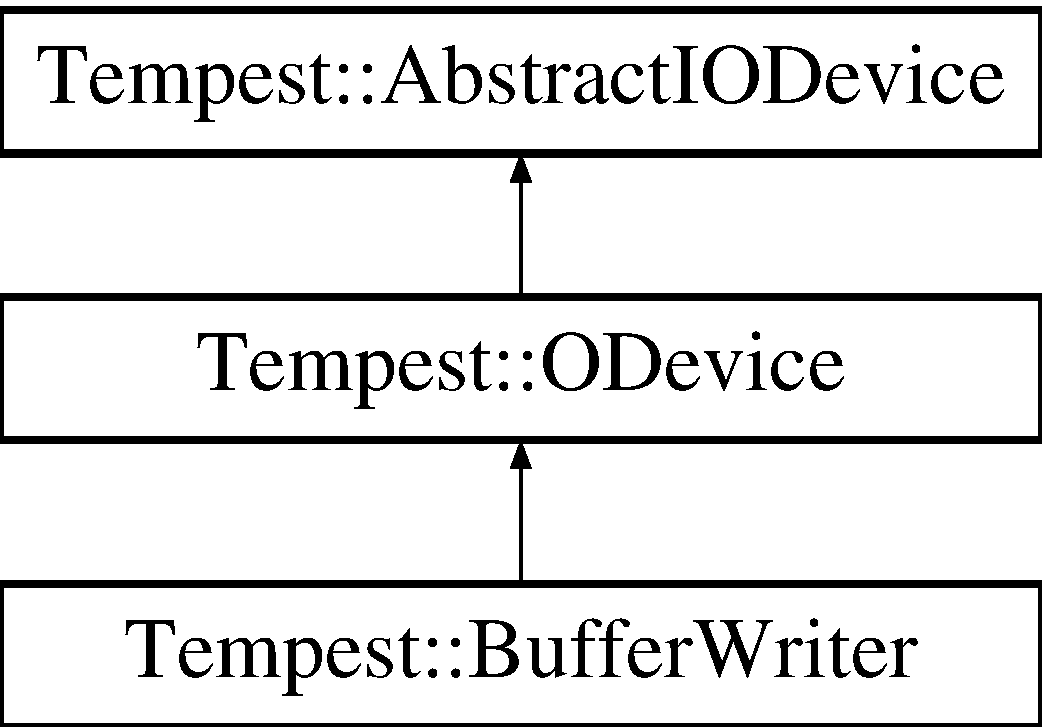
\includegraphics[height=3.000000cm]{class_tempest_1_1_buffer_writer}
\end{center}
\end{figure}
\subsection*{Public Member Functions}
\begin{DoxyCompactItemize}
\item 
\hypertarget{class_tempest_1_1_buffer_writer_a3f12ab32e9db8dff08d748c71b5d3f73}{{\bfseries Buffer\+Writer} (std\+::vector$<$ char $>$ \&vec)}\label{class_tempest_1_1_buffer_writer_a3f12ab32e9db8dff08d748c71b5d3f73}

\item 
\hypertarget{class_tempest_1_1_buffer_writer_a8301482bb39483279fcf58a4badb6753}{size\+\_\+t {\bfseries write\+Data} (const char $\ast$src, size\+\_\+t count)}\label{class_tempest_1_1_buffer_writer_a8301482bb39483279fcf58a4badb6753}

\end{DoxyCompactItemize}


The documentation for this class was generated from the following files\+:\begin{DoxyCompactItemize}
\item 
io/buffer.\+h\item 
io/buffer.\+cpp\end{DoxyCompactItemize}

\hypertarget{class_tempest_1_1_camera}{\section{Tempest\+:\+:Camera Class Reference}
\label{class_tempest_1_1_camera}\index{Tempest\+::\+Camera@{Tempest\+::\+Camera}}
}
Inheritance diagram for Tempest\+:\+:Camera\+:\begin{figure}[H]
\begin{center}
\leavevmode
\includegraphics[height=2.000000cm]{class_tempest_1_1_camera}
\end{center}
\end{figure}
\subsection*{Public Member Functions}
\begin{DoxyCompactItemize}
\item 
\hypertarget{class_tempest_1_1_camera_a44bd29c078f3f6d4fb56376a37211779}{virtual \hyperlink{class_tempest_1_1_matrix4x4}{Matrix4x4} {\bfseries view} () const }\label{class_tempest_1_1_camera_a44bd29c078f3f6d4fb56376a37211779}

\item 
\hypertarget{class_tempest_1_1_camera_af4815c6e3aa3d8de701e327c7ef8a9fd}{virtual \hyperlink{class_tempest_1_1_matrix4x4}{Matrix4x4} {\bfseries projective} () const }\label{class_tempest_1_1_camera_af4815c6e3aa3d8de701e327c7ef8a9fd}

\item 
\hypertarget{class_tempest_1_1_camera_a13e7a9058a07ae04ea016aabd0c4e693}{void {\bfseries set\+Spin\+X} (double x)}\label{class_tempest_1_1_camera_a13e7a9058a07ae04ea016aabd0c4e693}

\item 
\hypertarget{class_tempest_1_1_camera_a99739f91e38080e596a4aeca647dfe0b}{void {\bfseries set\+Spin\+Y} (double y)}\label{class_tempest_1_1_camera_a99739f91e38080e596a4aeca647dfe0b}

\item 
\hypertarget{class_tempest_1_1_camera_a322e3844448868a906cc0d62c68b0e28}{void {\bfseries set\+Zoom} (double z)}\label{class_tempest_1_1_camera_a322e3844448868a906cc0d62c68b0e28}

\item 
\hypertarget{class_tempest_1_1_camera_ab2a1ff22c62a3b7a222b4aa8672fbdfa}{double {\bfseries spin\+X} () const }\label{class_tempest_1_1_camera_ab2a1ff22c62a3b7a222b4aa8672fbdfa}

\item 
\hypertarget{class_tempest_1_1_camera_a448242b8a3f973e65aaa45644f15bc23}{double {\bfseries spin\+Y} () const }\label{class_tempest_1_1_camera_a448242b8a3f973e65aaa45644f15bc23}

\item 
\hypertarget{class_tempest_1_1_camera_a302899186cd76704ee37552716c9f4b5}{double {\bfseries zoom} () const }\label{class_tempest_1_1_camera_a302899186cd76704ee37552716c9f4b5}

\item 
\hypertarget{class_tempest_1_1_camera_a76837413bfb55455f0673b297bd6faf2}{void {\bfseries set\+Perspective} (bool use, int w=1, int h=1)}\label{class_tempest_1_1_camera_a76837413bfb55455f0673b297bd6faf2}

\item 
\hypertarget{class_tempest_1_1_camera_ae49e2ccc417e30fd5f3789c313799a47}{void {\bfseries set\+Perspective} (int w, int h, float use=45.\+0, float zmin=0.\+1f, float zmax=100.\+0f)}\label{class_tempest_1_1_camera_ae49e2ccc417e30fd5f3789c313799a47}

\item 
\hypertarget{class_tempest_1_1_camera_a7c269eb6d37c53273435590e398880f9}{void {\bfseries set\+Position} (double x, double y, double z)}\label{class_tempest_1_1_camera_a7c269eb6d37c53273435590e398880f9}

\item 
\hypertarget{class_tempest_1_1_camera_a7b41b23ec5a1af3fd6940919831c4669}{double {\bfseries x} () const }\label{class_tempest_1_1_camera_a7b41b23ec5a1af3fd6940919831c4669}

\item 
\hypertarget{class_tempest_1_1_camera_a1c0b071cbcef5421f102eee20cfd3cb8}{double {\bfseries y} () const }\label{class_tempest_1_1_camera_a1c0b071cbcef5421f102eee20cfd3cb8}

\item 
\hypertarget{class_tempest_1_1_camera_ae588fa9fbb424d1c04c9b1026fe68f5d}{double {\bfseries z} () const }\label{class_tempest_1_1_camera_ae588fa9fbb424d1c04c9b1026fe68f5d}

\item 
\hypertarget{class_tempest_1_1_camera_a4e3d9d06d4cf59d5d49674bd3af57e61}{void {\bfseries set\+Distance} (double d)}\label{class_tempest_1_1_camera_a4e3d9d06d4cf59d5d49674bd3af57e61}

\item 
\hypertarget{class_tempest_1_1_camera_a260df29ca84b944cc3e6c1281b1a9caf}{double {\bfseries distance} () const }\label{class_tempest_1_1_camera_a260df29ca84b944cc3e6c1281b1a9caf}

\end{DoxyCompactItemize}


The documentation for this class was generated from the following files\+:\begin{DoxyCompactItemize}
\item 
scene/camera.\+h\item 
scene/camera.\+cpp\end{DoxyCompactItemize}

\hypertarget{struct_tempest_1_1_abstract_a_p_i_1_1_caps}{\section{Tempest\+:\+:Abstract\+A\+P\+I\+:\+:Caps Struct Reference}
\label{struct_tempest_1_1_abstract_a_p_i_1_1_caps}\index{Tempest\+::\+Abstract\+A\+P\+I\+::\+Caps@{Tempest\+::\+Abstract\+A\+P\+I\+::\+Caps}}
}
\subsection*{Public Attributes}
\begin{DoxyCompactItemize}
\item 
\hypertarget{struct_tempest_1_1_abstract_a_p_i_1_1_caps_a8651f8e59059284d19e9bf8bf8bd92af}{int {\bfseries max\+Texture\+Size}}\label{struct_tempest_1_1_abstract_a_p_i_1_1_caps_a8651f8e59059284d19e9bf8bf8bd92af}

\item 
\hypertarget{struct_tempest_1_1_abstract_a_p_i_1_1_caps_aacf8c01ce6c88cb6e7cee01e65860ff3}{int {\bfseries max\+R\+T\+Count}}\label{struct_tempest_1_1_abstract_a_p_i_1_1_caps_aacf8c01ce6c88cb6e7cee01e65860ff3}

\item 
\hypertarget{struct_tempest_1_1_abstract_a_p_i_1_1_caps_a6bd176798eb3d9379b3437cb646c4bd2}{int {\bfseries max\+Varying\+Vectors}}\label{struct_tempest_1_1_abstract_a_p_i_1_1_caps_a6bd176798eb3d9379b3437cb646c4bd2}

\item 
\hypertarget{struct_tempest_1_1_abstract_a_p_i_1_1_caps_a9326d1499426d98a4811a712fb147a27}{int {\bfseries max\+Varying\+Components}}\label{struct_tempest_1_1_abstract_a_p_i_1_1_caps_a9326d1499426d98a4811a712fb147a27}

\item 
\hypertarget{struct_tempest_1_1_abstract_a_p_i_1_1_caps_a9b4d24f75da14d595004d3b631dfe72c}{bool {\bfseries has\+Half2}}\label{struct_tempest_1_1_abstract_a_p_i_1_1_caps_a9b4d24f75da14d595004d3b631dfe72c}

\item 
\hypertarget{struct_tempest_1_1_abstract_a_p_i_1_1_caps_af947c21a33308ced2bd40c2e35f22b7b}{bool {\bfseries has\+Half4}}\label{struct_tempest_1_1_abstract_a_p_i_1_1_caps_af947c21a33308ced2bd40c2e35f22b7b}

\item 
\hypertarget{struct_tempest_1_1_abstract_a_p_i_1_1_caps_a7ec5d9b3401454081497430d62e3aac9}{bool {\bfseries has3\+D\+Texture}}\label{struct_tempest_1_1_abstract_a_p_i_1_1_caps_a7ec5d9b3401454081497430d62e3aac9}

\item 
\hypertarget{struct_tempest_1_1_abstract_a_p_i_1_1_caps_a93562601517403668483bdfd31d8f776}{bool {\bfseries has\+Npot\+Texture}}\label{struct_tempest_1_1_abstract_a_p_i_1_1_caps_a93562601517403668483bdfd31d8f776}

\item 
\hypertarget{struct_tempest_1_1_abstract_a_p_i_1_1_caps_a19677bf2615d729b46a67361efcb9486}{bool {\bfseries has\+Redable\+Depth}}\label{struct_tempest_1_1_abstract_a_p_i_1_1_caps_a19677bf2615d729b46a67361efcb9486}

\end{DoxyCompactItemize}


The documentation for this struct was generated from the following file\+:\begin{DoxyCompactItemize}
\item 
core/abstractapi.\+h\end{DoxyCompactItemize}

\hypertarget{class_tempest_1_1_cg_dx9}{\section{Tempest\+:\+:Cg\+Dx9 Class Reference}
\label{class_tempest_1_1_cg_dx9}\index{Tempest\+::\+Cg\+Dx9@{Tempest\+::\+Cg\+Dx9}}
}
Inheritance diagram for Tempest\+:\+:Cg\+Dx9\+:\begin{figure}[H]
\begin{center}
\leavevmode
\includegraphics[height=3.000000cm]{class_tempest_1_1_cg_dx9}
\end{center}
\end{figure}
\subsection*{Classes}
\begin{DoxyCompactItemize}
\item 
struct \hyperlink{struct_cg_dx9_1_1_data}{Data}
\end{DoxyCompactItemize}
\subsection*{Public Member Functions}
\begin{DoxyCompactItemize}
\item 
\hypertarget{class_tempest_1_1_cg_dx9_ae00dd2a61f6ee4eac03c4fab4defd0ea}{{\bfseries Cg\+Dx9} (Abstract\+A\+P\+I\+::\+Direct\+X9\+Device $\ast$dev)}\label{class_tempest_1_1_cg_dx9_ae00dd2a61f6ee4eac03c4fab4defd0ea}

\item 
\hypertarget{class_tempest_1_1_cg_dx9_ac10056402c26eac8911b532b838008b1}{void {\bfseries enable} () const }\label{class_tempest_1_1_cg_dx9_ac10056402c26eac8911b532b838008b1}

\item 
\hypertarget{class_tempest_1_1_cg_dx9_ad0baf34ac3ac1e4b82805cde272c0425}{void {\bfseries bind} (const \hyperlink{class_tempest_1_1_vertex_shader}{Tempest\+::\+Vertex\+Shader} \&) const }\label{class_tempest_1_1_cg_dx9_ad0baf34ac3ac1e4b82805cde272c0425}

\item 
\hypertarget{class_tempest_1_1_cg_dx9_ad3196b4941c97f5058034b31b97dfa41}{void {\bfseries bind} (const \hyperlink{class_tempest_1_1_fragment_shader}{Tempest\+::\+Fragment\+Shader} \&) const }\label{class_tempest_1_1_cg_dx9_ad3196b4941c97f5058034b31b97dfa41}

\item 
\hypertarget{class_tempest_1_1_cg_dx9_a54890451df72d9ab4ca6c70b3683d112}{void {\bfseries un\+Bind} (const \hyperlink{class_tempest_1_1_vertex_shader}{Tempest\+::\+Vertex\+Shader} \&) const }\label{class_tempest_1_1_cg_dx9_a54890451df72d9ab4ca6c70b3683d112}

\item 
\hypertarget{class_tempest_1_1_cg_dx9_ac9b9f5f08758c0d2a556ca750370024c}{void {\bfseries un\+Bind} (const \hyperlink{class_tempest_1_1_fragment_shader}{Tempest\+::\+Fragment\+Shader} \&) const }\label{class_tempest_1_1_cg_dx9_ac9b9f5f08758c0d2a556ca750370024c}

\item 
\hypertarget{class_tempest_1_1_cg_dx9_ab39c2c66273eba2496806a76381eb741}{void $\ast$ {\bfseries context} () const }\label{class_tempest_1_1_cg_dx9_ab39c2c66273eba2496806a76381eb741}

\item 
\hypertarget{class_tempest_1_1_cg_dx9_abb2454f52bbe6c813d6da3dfc6a2a942}{\hyperlink{class_tempest_1_1_vertex_shader}{Vertex\+Shader} $\ast$ {\bfseries create\+Vertex\+Shader\+From\+Source} (const std\+::string \&src, std\+::string \&output\+Log) const }\label{class_tempest_1_1_cg_dx9_abb2454f52bbe6c813d6da3dfc6a2a942}

\item 
\hypertarget{class_tempest_1_1_cg_dx9_a253f193625fc35929d56477d36fdbfa4}{void {\bfseries delete\+Vertex\+Shader} (\hyperlink{class_tempest_1_1_vertex_shader}{Vertex\+Shader} $\ast$s) const }\label{class_tempest_1_1_cg_dx9_a253f193625fc35929d56477d36fdbfa4}

\item 
\hypertarget{class_tempest_1_1_cg_dx9_acb12670c11cbc823d74549a0caf8e229}{\hyperlink{class_tempest_1_1_fragment_shader}{Fragment\+Shader} $\ast$ {\bfseries create\+Fragment\+Shader\+From\+Source} (const std\+::string \&src, std\+::string \&output\+Log) const }\label{class_tempest_1_1_cg_dx9_acb12670c11cbc823d74549a0caf8e229}

\item 
\hypertarget{class_tempest_1_1_cg_dx9_a0ec6f19e3daa42041781c2b32f4f6f1c}{void {\bfseries delete\+Fragment\+Shader} (\hyperlink{class_tempest_1_1_fragment_shader}{Fragment\+Shader} $\ast$s) const }\label{class_tempest_1_1_cg_dx9_a0ec6f19e3daa42041781c2b32f4f6f1c}

\item 
\hypertarget{class_tempest_1_1_cg_dx9_a7d3eceb512c46c9cc1044e55ba29f0dc}{std\+::string {\bfseries surface\+Shader} (Shader\+Type t, const \hyperlink{struct_tempest_1_1_abstract_shading_lang_1_1_ui_shader_opt}{Ui\+Shader\+Opt} \&, bool \&has\+Halfpix\+Offset) const }\label{class_tempest_1_1_cg_dx9_a7d3eceb512c46c9cc1044e55ba29f0dc}

\end{DoxyCompactItemize}
\subsection*{Additional Inherited Members}


The documentation for this class was generated from the following files\+:\begin{DoxyCompactItemize}
\item 
dx/cgdx9.\+h\item 
dx/cgdx9.\+cpp\end{DoxyCompactItemize}

\hypertarget{struct_tempest_1_1_shader_input_1_1_chunk}{\section{Tempest\+:\+:Shader\+Input\+:\+:Chunk$<$ T $>$ Struct Template Reference}
\label{struct_tempest_1_1_shader_input_1_1_chunk}\index{Tempest\+::\+Shader\+Input\+::\+Chunk$<$ T $>$@{Tempest\+::\+Shader\+Input\+::\+Chunk$<$ T $>$}}
}
\subsection*{Public Member Functions}
\begin{DoxyCompactItemize}
\item 
\hypertarget{struct_tempest_1_1_shader_input_1_1_chunk_ac23fd7c6fef14a4a5d48bf5dea9d1b04}{void {\bfseries set} (const char $\ast$name, const T \&t)}\label{struct_tempest_1_1_shader_input_1_1_chunk_ac23fd7c6fef14a4a5d48bf5dea9d1b04}

\item 
\hypertarget{struct_tempest_1_1_shader_input_1_1_chunk_abb431b93730e9a70286a965ba9237944}{void {\bfseries reset\+I\+D} () const }\label{struct_tempest_1_1_shader_input_1_1_chunk_abb431b93730e9a70286a965ba9237944}

\end{DoxyCompactItemize}
\subsection*{Public Attributes}
\begin{DoxyCompactItemize}
\item 
\hypertarget{struct_tempest_1_1_shader_input_1_1_chunk_ad43bbeb5b9e5fb426b7b239269663e5e}{std\+::vector$<$ std\+::string $>$ {\bfseries names}}\label{struct_tempest_1_1_shader_input_1_1_chunk_ad43bbeb5b9e5fb426b7b239269663e5e}

\item 
\hypertarget{struct_tempest_1_1_shader_input_1_1_chunk_a3c012d4488bfab80fe74714a839f17c5}{std\+::vector$<$ T $>$ {\bfseries values}}\label{struct_tempest_1_1_shader_input_1_1_chunk_a3c012d4488bfab80fe74714a839f17c5}

\item 
\hypertarget{struct_tempest_1_1_shader_input_1_1_chunk_a32f8115938485065f050b490e82a81d8}{std\+::vector$<$ int32\+\_\+t $>$ {\bfseries id}}\label{struct_tempest_1_1_shader_input_1_1_chunk_a32f8115938485065f050b490e82a81d8}

\end{DoxyCompactItemize}


The documentation for this struct was generated from the following file\+:\begin{DoxyCompactItemize}
\item 
shading/shaderinput.\+h\end{DoxyCompactItemize}

\hypertarget{struct_tempest_1_1_abstract_texture_1_1_clamp_mode}{\section{Tempest\+:\+:Abstract\+Texture\+:\+:Clamp\+Mode Struct Reference}
\label{struct_tempest_1_1_abstract_texture_1_1_clamp_mode}\index{Tempest\+::\+Abstract\+Texture\+::\+Clamp\+Mode@{Tempest\+::\+Abstract\+Texture\+::\+Clamp\+Mode}}
}
\subsection*{Public Types}
\begin{DoxyCompactItemize}
\item 
\hypertarget{struct_tempest_1_1_abstract_texture_1_1_clamp_mode_a48849804d7d26fa1588769fca3128b17}{enum {\bfseries Type} \{ \\*
{\bfseries Clamp}, 
{\bfseries Clamp\+To\+Border}, 
{\bfseries Clamp\+To\+Edge}, 
{\bfseries Mirrored\+Repeat}, 
\\*
{\bfseries Repeat}, 
{\bfseries Count}
 \}}\label{struct_tempest_1_1_abstract_texture_1_1_clamp_mode_a48849804d7d26fa1588769fca3128b17}

\end{DoxyCompactItemize}


The documentation for this struct was generated from the following file\+:\begin{DoxyCompactItemize}
\item 
core/wrappers/abstracttexture.\+h\end{DoxyCompactItemize}

\hypertarget{class_tempest_1_1_close_event}{\section{Tempest\+:\+:Close\+Event Class Reference}
\label{class_tempest_1_1_close_event}\index{Tempest\+::\+Close\+Event@{Tempest\+::\+Close\+Event}}
}
Inheritance diagram for Tempest\+:\+:Close\+Event\+:\begin{figure}[H]
\begin{center}
\leavevmode
\includegraphics[height=2.000000cm]{class_tempest_1_1_close_event}
\end{center}
\end{figure}
\subsection*{Additional Inherited Members}


The documentation for this class was generated from the following file\+:\begin{DoxyCompactItemize}
\item 
ui/event.\+h\end{DoxyCompactItemize}

\hypertarget{class_tempest_1_1_color}{\section{Tempest\+:\+:Color Class Reference}
\label{class_tempest_1_1_color}\index{Tempest\+::\+Color@{Tempest\+::\+Color}}
}


Цвет, rgba, \mbox{[}0..1\mbox{]}, одинарная точность.  




{\ttfamily \#include $<$color.\+h$>$}

\subsection*{Public Member Functions}
\begin{DoxyCompactItemize}
\item 
\hypertarget{class_tempest_1_1_color_a9a742cbe9f9f4037f5d9f4e81a9b2428}{\hyperlink{class_tempest_1_1_color_a9a742cbe9f9f4037f5d9f4e81a9b2428}{Color} ()}\label{class_tempest_1_1_color_a9a742cbe9f9f4037f5d9f4e81a9b2428}

\begin{DoxyCompactList}\small\item\em Констуктор. Эквивалентно \hyperlink{class_tempest_1_1_color}{Color}(1.\+0). \end{DoxyCompactList}\item 
\hypertarget{class_tempest_1_1_color_a4570f17f449c0302fd4c2964989ff65d}{\hyperlink{class_tempest_1_1_color_a4570f17f449c0302fd4c2964989ff65d}{Color} (float rgba)}\label{class_tempest_1_1_color_a4570f17f449c0302fd4c2964989ff65d}

\begin{DoxyCompactList}\small\item\em Тоже конструктор. Всем каналам будет задано значение rgba. \end{DoxyCompactList}\item 
\hypertarget{class_tempest_1_1_color_a1ff48fafaffb35cdbf0d8384fc48e7e9}{\hyperlink{class_tempest_1_1_color_a1ff48fafaffb35cdbf0d8384fc48e7e9}{Color} (float \hyperlink{class_tempest_1_1_color_ad6d7d14e2251970ddc32a3845c2adc46}{r}, float \hyperlink{class_tempest_1_1_color_a7dd31a26074d75037eb72979d11f9a87}{g}, float \hyperlink{class_tempest_1_1_color_a3c9641a1dee2770f28c167ff6866158c}{b}, float \hyperlink{class_tempest_1_1_color_ac36ada4151d5898dea335ebf8b1cd21b}{a}=1.\+0)}\label{class_tempest_1_1_color_a1ff48fafaffb35cdbf0d8384fc48e7e9}

\begin{DoxyCompactList}\small\item\em Конструктор. \end{DoxyCompactList}\item 
\hypertarget{class_tempest_1_1_color_ac527f9b3cd41835585b31767b44cf6a9}{void \hyperlink{class_tempest_1_1_color_ac527f9b3cd41835585b31767b44cf6a9}{set} (float \hyperlink{class_tempest_1_1_color_ad6d7d14e2251970ddc32a3845c2adc46}{r}, float \hyperlink{class_tempest_1_1_color_a7dd31a26074d75037eb72979d11f9a87}{g}, float \hyperlink{class_tempest_1_1_color_a3c9641a1dee2770f28c167ff6866158c}{b}, float \hyperlink{class_tempest_1_1_color_ac36ada4151d5898dea335ebf8b1cd21b}{a})}\label{class_tempest_1_1_color_ac527f9b3cd41835585b31767b44cf6a9}

\begin{DoxyCompactList}\small\item\em Задание всех каналов явно. \end{DoxyCompactList}\item 
\hypertarget{class_tempest_1_1_color_a8d94f6e9cabde79faeb5b8a7391c3101}{void \hyperlink{class_tempest_1_1_color_a8d94f6e9cabde79faeb5b8a7391c3101}{set} (float rgba)}\label{class_tempest_1_1_color_a8d94f6e9cabde79faeb5b8a7391c3101}

\begin{DoxyCompactList}\small\item\em Перегруженная функция, введена для удобства. \end{DoxyCompactList}\item 
const float $\ast$ \hyperlink{class_tempest_1_1_color_a6e3131e891489f4df3b46dc0b3a8c344}{data} () const 
\item 
\hypertarget{class_tempest_1_1_color_a5ec3c2546dae446433c59fbdf400ef65}{\hyperlink{class_tempest_1_1_color}{Color} \& \hyperlink{class_tempest_1_1_color_a5ec3c2546dae446433c59fbdf400ef65}{operator=} (const \hyperlink{class_tempest_1_1_color}{Color} \&other)}\label{class_tempest_1_1_color_a5ec3c2546dae446433c59fbdf400ef65}

\begin{DoxyCompactList}\small\item\em Присваивание. \end{DoxyCompactList}\item 
\hypertarget{class_tempest_1_1_color_ad2da29b884581b6601b9cf524228cb7d}{\hyperlink{class_tempest_1_1_color}{Color} \hyperlink{class_tempest_1_1_color_ad2da29b884581b6601b9cf524228cb7d}{operator+} (const \hyperlink{class_tempest_1_1_color}{Color} \&other)}\label{class_tempest_1_1_color_ad2da29b884581b6601b9cf524228cb7d}

\begin{DoxyCompactList}\small\item\em Сложение. Результат не будет обрубаться по диапозону. \end{DoxyCompactList}\item 
\hypertarget{class_tempest_1_1_color_aa00513416acac8489d70fd27b78b81af}{\hyperlink{class_tempest_1_1_color}{Color} \hyperlink{class_tempest_1_1_color_aa00513416acac8489d70fd27b78b81af}{operator-\/} (const \hyperlink{class_tempest_1_1_color}{Color} \&other)}\label{class_tempest_1_1_color_aa00513416acac8489d70fd27b78b81af}

\begin{DoxyCompactList}\small\item\em Вычитание. Результат не будет обрубаться по диапозону. \end{DoxyCompactList}\item 
\hypertarget{class_tempest_1_1_color_ac283f565588e93af17866d357827fa87}{void \hyperlink{class_tempest_1_1_color_ac283f565588e93af17866d357827fa87}{operator+=} (const \hyperlink{class_tempest_1_1_color}{Color} \&other)}\label{class_tempest_1_1_color_ac283f565588e93af17866d357827fa87}

\begin{DoxyCompactList}\small\item\em Сложение. Результат не будет обрубаться по диапозону. \end{DoxyCompactList}\item 
\hypertarget{class_tempest_1_1_color_aa058fd5b4366eaaf053d0cda3837c9a5}{void \hyperlink{class_tempest_1_1_color_aa058fd5b4366eaaf053d0cda3837c9a5}{operator-\/=} (const \hyperlink{class_tempest_1_1_color}{Color} \&other)}\label{class_tempest_1_1_color_aa058fd5b4366eaaf053d0cda3837c9a5}

\begin{DoxyCompactList}\small\item\em Вычитание. Результат не будет обрубаться по диапозону. \end{DoxyCompactList}\item 
\hypertarget{class_tempest_1_1_color_ad6d7d14e2251970ddc32a3845c2adc46}{float \hyperlink{class_tempest_1_1_color_ad6d7d14e2251970ddc32a3845c2adc46}{r} () const }\label{class_tempest_1_1_color_ad6d7d14e2251970ddc32a3845c2adc46}

\begin{DoxyCompactList}\small\item\em Канал red. \end{DoxyCompactList}\item 
\hypertarget{class_tempest_1_1_color_a7dd31a26074d75037eb72979d11f9a87}{float \hyperlink{class_tempest_1_1_color_a7dd31a26074d75037eb72979d11f9a87}{g} () const }\label{class_tempest_1_1_color_a7dd31a26074d75037eb72979d11f9a87}

\begin{DoxyCompactList}\small\item\em Канал green. \end{DoxyCompactList}\item 
\hypertarget{class_tempest_1_1_color_a3c9641a1dee2770f28c167ff6866158c}{float \hyperlink{class_tempest_1_1_color_a3c9641a1dee2770f28c167ff6866158c}{b} () const }\label{class_tempest_1_1_color_a3c9641a1dee2770f28c167ff6866158c}

\begin{DoxyCompactList}\small\item\em Канал blue. \end{DoxyCompactList}\item 
\hypertarget{class_tempest_1_1_color_ac36ada4151d5898dea335ebf8b1cd21b}{float \hyperlink{class_tempest_1_1_color_ac36ada4151d5898dea335ebf8b1cd21b}{a} () const }\label{class_tempest_1_1_color_ac36ada4151d5898dea335ebf8b1cd21b}

\begin{DoxyCompactList}\small\item\em alpha канал. \end{DoxyCompactList}\item 
\hypertarget{class_tempest_1_1_color_a530574bfdce44ddb000245e06eb8788a}{float \& {\bfseries operator\mbox{[}$\,$\mbox{]}} (int i)}\label{class_tempest_1_1_color_a530574bfdce44ddb000245e06eb8788a}

\item 
\hypertarget{class_tempest_1_1_color_a68ec7fa2525d944737a4288d7125734e}{const float \& {\bfseries operator\mbox{[}$\,$\mbox{]}} (int i) const }\label{class_tempest_1_1_color_a68ec7fa2525d944737a4288d7125734e}

\item 
\hypertarget{class_tempest_1_1_color_a4e3847141a90051eb9db797a82a6aa3a}{bool {\bfseries operator==} (const \hyperlink{class_tempest_1_1_color}{Color} \&other) const }\label{class_tempest_1_1_color_a4e3847141a90051eb9db797a82a6aa3a}

\item 
\hypertarget{class_tempest_1_1_color_a6763dbfc1d7592a1476bee33c98cdf24}{bool {\bfseries operator!=} (const \hyperlink{class_tempest_1_1_color}{Color} \&other) const }\label{class_tempest_1_1_color_a6763dbfc1d7592a1476bee33c98cdf24}

\end{DoxyCompactItemize}


\subsection{Detailed Description}
Цвет, rgba, \mbox{[}0..1\mbox{]}, одинарная точность. \begin{Desc}
\item[Examples\+: ]\par
\hyperlink{_cube_2mainwindow_8cpp-example}{Cube/mainwindow.\+cpp}, and \hyperlink{_painting2d_2mainwindow_8cpp-example}{Painting2d/mainwindow.\+cpp}.\end{Desc}


\subsection{Member Function Documentation}
\hypertarget{class_tempest_1_1_color_a6e3131e891489f4df3b46dc0b3a8c344}{\index{Tempest\+::\+Color@{Tempest\+::\+Color}!data@{data}}
\index{data@{data}!Tempest\+::\+Color@{Tempest\+::\+Color}}
\subsubsection[{data}]{\setlength{\rightskip}{0pt plus 5cm}const float $\ast$ Color\+::data (
\begin{DoxyParamCaption}
{}
\end{DoxyParamCaption}
) const}}\label{class_tempest_1_1_color_a6e3131e891489f4df3b46dc0b3a8c344}
Получить 4х элементный массив, элементы которого являются значениями каналов. 

The documentation for this class was generated from the following files\+:\begin{DoxyCompactItemize}
\item 
utils/color.\+h\item 
utils/color.\+cpp\end{DoxyCompactItemize}

\hypertarget{struct_tempest_1_1_jpeg_codec_1_1compress}{\section{Tempest\+:\+:Jpeg\+Codec\+:\+:compress Struct Reference}
\label{struct_tempest_1_1_jpeg_codec_1_1compress}\index{Tempest\+::\+Jpeg\+Codec\+::compress@{Tempest\+::\+Jpeg\+Codec\+::compress}}
}
Inheritance diagram for Tempest\+:\+:Jpeg\+Codec\+:\+:compress\+:\begin{figure}[H]
\begin{center}
\leavevmode
\includegraphics[height=2.000000cm]{struct_tempest_1_1_jpeg_codec_1_1compress}
\end{center}
\end{figure}
\subsection*{Public Member Functions}
\begin{DoxyCompactItemize}
\item 
\hypertarget{struct_tempest_1_1_jpeg_codec_1_1compress_a78443bef7f4972c27822550c53c9b97e}{void {\bfseries start} ()}\label{struct_tempest_1_1_jpeg_codec_1_1compress_a78443bef7f4972c27822550c53c9b97e}

\end{DoxyCompactItemize}


The documentation for this struct was generated from the following file\+:\begin{DoxyCompactItemize}
\item 
core/imagecodec.\+cpp\end{DoxyCompactItemize}

\hypertarget{struct_tempest_1_1_system_a_p_i_1_1_cpu_info}{\section{Tempest\+:\+:System\+A\+P\+I\+:\+:Cpu\+Info Struct Reference}
\label{struct_tempest_1_1_system_a_p_i_1_1_cpu_info}\index{Tempest\+::\+System\+A\+P\+I\+::\+Cpu\+Info@{Tempest\+::\+System\+A\+P\+I\+::\+Cpu\+Info}}
}
\subsection*{Public Attributes}
\begin{DoxyCompactItemize}
\item 
\hypertarget{struct_tempest_1_1_system_a_p_i_1_1_cpu_info_a6f11f2be01af875bbce7c5a235a31727}{int {\bfseries cpu\+Count}}\label{struct_tempest_1_1_system_a_p_i_1_1_cpu_info_a6f11f2be01af875bbce7c5a235a31727}

\end{DoxyCompactItemize}


The documentation for this struct was generated from the following file\+:\begin{DoxyCompactItemize}
\item 
system/systemapi.\+h\end{DoxyCompactItemize}

\hypertarget{struct_tempest_1_1_render_state_1_1_cull_mode}{\section{Tempest\+:\+:Render\+State\+:\+:Cull\+Mode Struct Reference}
\label{struct_tempest_1_1_render_state_1_1_cull_mode}\index{Tempest\+::\+Render\+State\+::\+Cull\+Mode@{Tempest\+::\+Render\+State\+::\+Cull\+Mode}}
}
\subsection*{Public Types}
\begin{DoxyCompactItemize}
\item 
\hypertarget{struct_tempest_1_1_render_state_1_1_cull_mode_a36b1a0fee8db3093624fe167bd1fceaa}{enum {\bfseries Type} \{ {\bfseries no\+Cull} = 0, 
{\bfseries front}, 
{\bfseries back}
 \}}\label{struct_tempest_1_1_render_state_1_1_cull_mode_a36b1a0fee8db3093624fe167bd1fceaa}

\end{DoxyCompactItemize}


The documentation for this struct was generated from the following file\+:\begin{DoxyCompactItemize}
\item 
core/renderstate.\+h\end{DoxyCompactItemize}

\hypertarget{class_tempest_1_1_custom_event}{\section{Tempest\+:\+:Custom\+Event Class Reference}
\label{class_tempest_1_1_custom_event}\index{Tempest\+::\+Custom\+Event@{Tempest\+::\+Custom\+Event}}
}
Inheritance diagram for Tempest\+:\+:Custom\+Event\+:\begin{figure}[H]
\begin{center}
\leavevmode
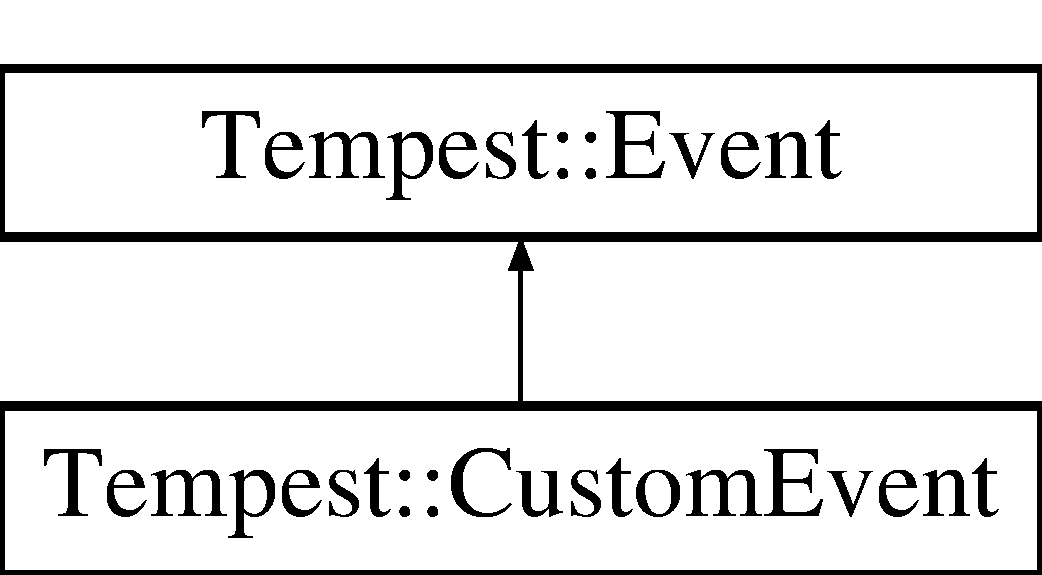
\includegraphics[height=2.000000cm]{class_tempest_1_1_custom_event}
\end{center}
\end{figure}
\subsection*{Additional Inherited Members}


The documentation for this class was generated from the following file\+:\begin{DoxyCompactItemize}
\item 
ui/event.\+h\end{DoxyCompactItemize}

\hypertarget{struct_g_l_s_l_1_1_data}{\section{Tempest\+:\+:G\+L\+S\+L\+:\+:Data Struct Reference}
\label{struct_g_l_s_l_1_1_data}\index{Tempest\+::\+G\+L\+S\+L\+::\+Data@{Tempest\+::\+G\+L\+S\+L\+::\+Data}}
}
\subsection*{Classes}
\begin{DoxyCompactItemize}
\item 
struct \hyperlink{struct_g_l_s_l_1_1_data_1_1_sh_program}{Sh\+Program}
\end{DoxyCompactItemize}
\subsection*{Public Member Functions}
\begin{DoxyCompactItemize}
\item 
\hypertarget{struct_g_l_s_l_1_1_data_a7943d8b7dcde0fd9d68790e71e143011}{void {\bfseries dbg} ()}\label{struct_g_l_s_l_1_1_data_a7943d8b7dcde0fd9d68790e71e143011}

\item 
\hypertarget{struct_g_l_s_l_1_1_data_a85d85fdbcdb1fbdbf40941027060cce8}{std\+::string {\bfseries read\+File} (const char $\ast$f)}\label{struct_g_l_s_l_1_1_data_a85d85fdbcdb1fbdbf40941027060cce8}

\item 
\hypertarget{struct_g_l_s_l_1_1_data_a2917ec68a8f68e1ef2bf579e76977bbc}{std\+::string {\bfseries read\+File} (const char16\+\_\+t $\ast$f)}\label{struct_g_l_s_l_1_1_data_a2917ec68a8f68e1ef2bf579e76977bbc}

\item 
\hypertarget{struct_g_l_s_l_1_1_data_a041d67fbcc79c1f014f5c7284768bd99}{G\+Luint {\bfseries load\+Shader} (G\+Lenum shader\+Type, const char $\ast$p\+Source, std\+::string \&log)}\label{struct_g_l_s_l_1_1_data_a041d67fbcc79c1f014f5c7284768bd99}

\item 
\hypertarget{struct_g_l_s_l_1_1_data_a87b3e1e29a4a24273bdd7d37c5c93f2d}{G\+Lint {\bfseries location} (G\+Luint prog, const char $\ast$name)}\label{struct_g_l_s_l_1_1_data_a87b3e1e29a4a24273bdd7d37c5c93f2d}

\item 
\hypertarget{struct_g_l_s_l_1_1_data_a8fa7fbcb36d9df16e527ac415f287c31}{{\footnotesize template$<$class Sampler $>$ }\\void {\bfseries setup\+Sampler} (G\+Lenum tex\+Class, G\+Lint prm, int slot, Detail\+::\+G\+L\+Texture $\ast$tx, const Sampler \&s)}\label{struct_g_l_s_l_1_1_data_a8fa7fbcb36d9df16e527ac415f287c31}

\item 
\hypertarget{struct_g_l_s_l_1_1_data_a7e3dccd454744f69dd4d147401bbe545}{Texture3d\+::\+Clamp\+Mode\+::\+Type {\bfseries clamp\+W} (const \hyperlink{struct_tempest_1_1_texture2d_1_1_sampler}{Texture2d\+::\+Sampler} \&)}\label{struct_g_l_s_l_1_1_data_a7e3dccd454744f69dd4d147401bbe545}

\item 
\hypertarget{struct_g_l_s_l_1_1_data_ab4875596e2a3845cbdcfe9253fdb6c98}{Texture3d\+::\+Clamp\+Mode\+::\+Type {\bfseries clamp\+W} (const \hyperlink{struct_tempest_1_1_texture3d_1_1_sampler}{Texture3d\+::\+Sampler} \&s)}\label{struct_g_l_s_l_1_1_data_ab4875596e2a3845cbdcfe9253fdb6c98}

\item 
\hypertarget{struct_g_l_s_l_1_1_data_abf9a0755cff785392b0ecb78e4f64a99}{bool {\bfseries is\+Anisotropic} (const \hyperlink{struct_tempest_1_1_texture2d_1_1_sampler}{Texture2d\+::\+Sampler} \&s)}\label{struct_g_l_s_l_1_1_data_abf9a0755cff785392b0ecb78e4f64a99}

\item 
\hypertarget{struct_g_l_s_l_1_1_data_a54093da67f84935fd573f3d336b8ca58}{bool {\bfseries is\+Anisotropic} (const \hyperlink{struct_tempest_1_1_texture3d_1_1_sampler}{Texture3d\+::\+Sampler} \&)}\label{struct_g_l_s_l_1_1_data_a54093da67f84935fd573f3d336b8ca58}

\item 
\hypertarget{struct_g_l_s_l_1_1_data_a5dc59d87cd79d431cd46a0cc9ee59c52}{G\+Luint {\bfseries link} (G\+Luint vertex\+Shader, G\+Luint pixel\+Shader, const Abstract\+A\+P\+I\+::\+Vertex\+Decl $\ast$vdecl, std\+::string $\ast$log)}\label{struct_g_l_s_l_1_1_data_a5dc59d87cd79d431cd46a0cc9ee59c52}

\end{DoxyCompactItemize}
\subsection*{Static Public Member Functions}
\begin{DoxyCompactItemize}
\item 
\hypertarget{struct_g_l_s_l_1_1_data_a948e262d20b78600bbf6305c1e229b15}{static void {\bfseries dbg\+Out} (G\+Luint)}\label{struct_g_l_s_l_1_1_data_a948e262d20b78600bbf6305c1e229b15}

\item 
\hypertarget{struct_g_l_s_l_1_1_data_a3dba8e7a31d32ce2f6bbd82048a7092a}{static void {\bfseries dbg} (bool, G\+Luint)}\label{struct_g_l_s_l_1_1_data_a3dba8e7a31d32ce2f6bbd82048a7092a}

\end{DoxyCompactItemize}
\subsection*{Public Attributes}
\begin{DoxyCompactItemize}
\item 
\hypertarget{struct_g_l_s_l_1_1_data_a3d3d0643bb9186f8c704c1f15d0f3520}{Abstract\+A\+P\+I\+::\+Open\+G\+L2x\+Device $\ast$ {\bfseries context}}\label{struct_g_l_s_l_1_1_data_a3d3d0643bb9186f8c704c1f15d0f3520}

\item 
\hypertarget{struct_g_l_s_l_1_1_data_a6d182278d047775ec684f1a9d5f61d9c}{float {\bfseries max\+Anisotropy}}\label{struct_g_l_s_l_1_1_data_a6d182278d047775ec684f1a9d5f61d9c}

\item 
\hypertarget{struct_g_l_s_l_1_1_data_ab1a68c470e6dfeb00bee9a085d9aa53a}{const \hyperlink{class_tempest_1_1_vertex_shader}{Tempest\+::\+Vertex\+Shader} $\ast$ {\bfseries current\+V\+S}}\label{struct_g_l_s_l_1_1_data_ab1a68c470e6dfeb00bee9a085d9aa53a}

\item 
\hypertarget{struct_g_l_s_l_1_1_data_a736c5875b2acece914a0c3ecd8388647}{const \hyperlink{class_tempest_1_1_fragment_shader}{Tempest\+::\+Fragment\+Shader} $\ast$ {\bfseries current\+F\+S}}\label{struct_g_l_s_l_1_1_data_a736c5875b2acece914a0c3ecd8388647}

\item 
\hypertarget{struct_g_l_s_l_1_1_data_a6098de439c3d34a52c7e289f367bacb0}{Detail\+::\+Uniform\+Cash$<$ G\+Luint $>$ {\bfseries u\+Cash}}\label{struct_g_l_s_l_1_1_data_a6098de439c3d34a52c7e289f367bacb0}

\item 
\hypertarget{struct_g_l_s_l_1_1_data_af8530277458194ebbb63c2b269977afa}{const Abstract\+A\+P\+I\+::\+Vertex\+Decl $\ast$ {\bfseries vdecl}}\label{struct_g_l_s_l_1_1_data_af8530277458194ebbb63c2b269977afa}

\item 
\hypertarget{struct_g_l_s_l_1_1_data_aa25eb965f8fd8e32ef988dd13bf83d65}{std\+::vector$<$ \hyperlink{struct_g_l_s_l_1_1_data_1_1_sh_program}{Sh\+Program} $>$ {\bfseries prog}}\label{struct_g_l_s_l_1_1_data_aa25eb965f8fd8e32ef988dd13bf83d65}

\item 
\hypertarget{struct_g_l_s_l_1_1_data_a47ea72984a4bca598d8236cc788bbf61}{bool {\bfseries has\+Anisotropic}}\label{struct_g_l_s_l_1_1_data_a47ea72984a4bca598d8236cc788bbf61}

\item 
\hypertarget{struct_g_l_s_l_1_1_data_a36b54e6f5801f6dd1c519cd0af8e6476}{\hyperlink{struct_g_l_s_l_1_1_data_1_1_sh_program}{Sh\+Program} {\bfseries cur\+Program}}\label{struct_g_l_s_l_1_1_data_a36b54e6f5801f6dd1c519cd0af8e6476}

\item 
\hypertarget{struct_g_l_s_l_1_1_data_a3c761e20f70f0990df17b4e30cd19db6}{char {\bfseries tex\+Attr\+Name} \mbox{[}14\mbox{]}}\label{struct_g_l_s_l_1_1_data_a3c761e20f70f0990df17b4e30cd19db6}

\item 
\hypertarget{struct_g_l_s_l_1_1_data_af6813ecdd7bc0027d76f9b173da815f5}{int32\+\_\+t {\bfseries not\+Id}}\label{struct_g_l_s_l_1_1_data_af6813ecdd7bc0027d76f9b173da815f5}

\end{DoxyCompactItemize}


The documentation for this struct was generated from the following file\+:\begin{DoxyCompactItemize}
\item 
ogl/glsl.\+cpp\end{DoxyCompactItemize}

\hypertarget{struct_index_buffer_holder_1_1_data}{\section{Tempest\+:\+:Index\+Buffer\+Holder\+:\+:Data Struct Reference}
\label{struct_index_buffer_holder_1_1_data}\index{Tempest\+::\+Index\+Buffer\+Holder\+::\+Data@{Tempest\+::\+Index\+Buffer\+Holder\+::\+Data}}
}
\subsection*{Classes}
\begin{DoxyCompactItemize}
\item 
struct \hyperlink{struct_index_buffer_holder_1_1_data_1_1_l_d_data}{L\+D\+Data}
\end{DoxyCompactItemize}
\subsection*{Public Types}
\begin{DoxyCompactItemize}
\item 
\hypertarget{struct_index_buffer_holder_1_1_data_a352c08519c48007e32628d8c0333a50f}{typedef std\+::unordered\+\_\+map\\*
$<$ Abstract\+A\+P\+I\+::\+Index\+Buffer \\*
$\ast$, \hyperlink{struct_index_buffer_holder_1_1_data_1_1_l_d_data}{L\+D\+Data} $\ast$ $>$\+::iterator {\bfseries Iterator}}\label{struct_index_buffer_holder_1_1_data_a352c08519c48007e32628d8c0333a50f}

\end{DoxyCompactItemize}
\subsection*{Public Attributes}
\begin{DoxyCompactItemize}
\item 
\hypertarget{struct_index_buffer_holder_1_1_data_acce28854207b44d5e4cb167bc5c7799b}{\hyperlink{struct_index_buffer_holder_1_1_data_1_1_l_d_data}{L\+D\+Data} {\bfseries no\+Data}}\label{struct_index_buffer_holder_1_1_data_acce28854207b44d5e4cb167bc5c7799b}

\item 
\hypertarget{struct_index_buffer_holder_1_1_data_a524f7eb8e3b979f91bfe652ebe19d0f0}{std\+::unordered\+\_\+map\\*
$<$ Abstract\+A\+P\+I\+::\+Index\+Buffer \\*
$\ast$, \hyperlink{struct_index_buffer_holder_1_1_data_1_1_l_d_data}{L\+D\+Data} $\ast$ $>$ {\bfseries ibos}}\label{struct_index_buffer_holder_1_1_data_a524f7eb8e3b979f91bfe652ebe19d0f0}

\item 
\hypertarget{struct_index_buffer_holder_1_1_data_a86c3dc33552feb31ba80c3d064fd1d6a}{std\+::unordered\+\_\+map\\*
$<$ Abstract\+A\+P\+I\+::\+Index\+Buffer \\*
$\ast$, \hyperlink{struct_index_buffer_holder_1_1_data_1_1_l_d_data}{L\+D\+Data} $\ast$ $>$ {\bfseries restore}}\label{struct_index_buffer_holder_1_1_data_a86c3dc33552feb31ba80c3d064fd1d6a}

\end{DoxyCompactItemize}


The documentation for this struct was generated from the following file\+:\begin{DoxyCompactItemize}
\item 
data\+Control/indexbufferholder.\+cpp\end{DoxyCompactItemize}

\hypertarget{struct_texture_holder_1_1_data}{\section{Tempest\+:\+:Texture\+Holder\+:\+:Data Struct Reference}
\label{struct_texture_holder_1_1_data}\index{Tempest\+::\+Texture\+Holder\+::\+Data@{Tempest\+::\+Texture\+Holder\+::\+Data}}
}
\subsection*{Classes}
\begin{DoxyCompactItemize}
\item 
struct \hyperlink{struct_texture_holder_1_1_data_1_1_dyn_texture}{Dyn\+Texture}
\item 
struct \hyperlink{struct_texture_holder_1_1_data_1_1_pixmap_texture}{Pixmap\+Texture}
\end{DoxyCompactItemize}
\subsection*{Public Member Functions}
\begin{DoxyCompactItemize}
\item 
\hypertarget{struct_texture_holder_1_1_data_a4e1dcbfa0aac476a979ec1c58edb1655}{void {\bfseries remove\+Tex} (Abstract\+A\+P\+I\+::\+Texture $\ast$t)}\label{struct_texture_holder_1_1_data_a4e1dcbfa0aac476a979ec1c58edb1655}

\end{DoxyCompactItemize}
\subsection*{Public Attributes}
\begin{DoxyCompactItemize}
\item 
\hypertarget{struct_texture_holder_1_1_data_a06c83385574f7da8ae9afd022a7000e9}{std\+::vector$<$ \hyperlink{struct_texture_holder_1_1_data_1_1_dyn_texture}{Dyn\+Texture} $>$ {\bfseries dynamic\+\_\+textures}}\label{struct_texture_holder_1_1_data_a06c83385574f7da8ae9afd022a7000e9}

\item 
\hypertarget{struct_texture_holder_1_1_data_a4ae87cab1aae94aa7f7837eee436e051}{std\+::vector$<$ \hyperlink{struct_texture_holder_1_1_data_1_1_pixmap_texture}{Pixmap\+Texture} $>$ {\bfseries pixmap\+\_\+textures}}\label{struct_texture_holder_1_1_data_a4ae87cab1aae94aa7f7837eee436e051}

\item 
\hypertarget{struct_texture_holder_1_1_data_a78565853ba4600957371d5c104f6ee6a}{size\+\_\+t {\bfseries count}}\label{struct_texture_holder_1_1_data_a78565853ba4600957371d5c104f6ee6a}

\end{DoxyCompactItemize}


The documentation for this struct was generated from the following file\+:\begin{DoxyCompactItemize}
\item 
data\+Control/textureholder.\+cpp\end{DoxyCompactItemize}

\hypertarget{struct_vertex_buffer_holder_1_1_data}{\section{Tempest\+:\+:Vertex\+Buffer\+Holder\+:\+:Data Struct Reference}
\label{struct_vertex_buffer_holder_1_1_data}\index{Tempest\+::\+Vertex\+Buffer\+Holder\+::\+Data@{Tempest\+::\+Vertex\+Buffer\+Holder\+::\+Data}}
}
\subsection*{Classes}
\begin{DoxyCompactItemize}
\item 
struct \hyperlink{struct_vertex_buffer_holder_1_1_data_1_1_l_d_data}{L\+D\+Data}
\end{DoxyCompactItemize}
\subsection*{Public Types}
\begin{DoxyCompactItemize}
\item 
\hypertarget{struct_vertex_buffer_holder_1_1_data_ada1ff4c2368f043aa670e337a34e8583}{typedef std\+::unordered\+\_\+map\\*
$<$ Abstract\+A\+P\+I\+::\+Vertex\+Buffer \\*
$\ast$, \hyperlink{struct_vertex_buffer_holder_1_1_data_1_1_l_d_data}{L\+D\+Data} $\ast$ $>$\+::iterator {\bfseries Iterator}}\label{struct_vertex_buffer_holder_1_1_data_ada1ff4c2368f043aa670e337a34e8583}

\end{DoxyCompactItemize}
\subsection*{Public Attributes}
\begin{DoxyCompactItemize}
\item 
\hypertarget{struct_vertex_buffer_holder_1_1_data_a9a0e80f75a785930b4d48a7afac0c7b1}{\hyperlink{struct_vertex_buffer_holder_1_1_data_1_1_l_d_data}{L\+D\+Data} {\bfseries no\+Data}}\label{struct_vertex_buffer_holder_1_1_data_a9a0e80f75a785930b4d48a7afac0c7b1}

\item 
\hypertarget{struct_vertex_buffer_holder_1_1_data_a77fa39e74d7cb941394b9a4c74a24d95}{std\+::unordered\+\_\+map\\*
$<$ Abstract\+A\+P\+I\+::\+Vertex\+Buffer \\*
$\ast$, \hyperlink{struct_vertex_buffer_holder_1_1_data_1_1_l_d_data}{L\+D\+Data} $\ast$ $>$ {\bfseries vbos}}\label{struct_vertex_buffer_holder_1_1_data_a77fa39e74d7cb941394b9a4c74a24d95}

\item 
\hypertarget{struct_vertex_buffer_holder_1_1_data_ae26dba46284f76e8a449355bdef4ffa0}{std\+::unordered\+\_\+map\\*
$<$ Abstract\+A\+P\+I\+::\+Vertex\+Buffer \\*
$\ast$, \hyperlink{struct_vertex_buffer_holder_1_1_data_1_1_l_d_data}{L\+D\+Data} $\ast$ $>$ {\bfseries restore}}\label{struct_vertex_buffer_holder_1_1_data_ae26dba46284f76e8a449355bdef4ffa0}

\end{DoxyCompactItemize}


The documentation for this struct was generated from the following file\+:\begin{DoxyCompactItemize}
\item 
data\+Control/vertexbufferholder.\+cpp\end{DoxyCompactItemize}

\hypertarget{struct_device_1_1_data}{\section{Tempest\+:\+:Device\+:\+:Data Struct Reference}
\label{struct_device_1_1_data}\index{Tempest\+::\+Device\+::\+Data@{Tempest\+::\+Device\+::\+Data}}
}
\subsection*{Classes}
\begin{DoxyCompactItemize}
\item 
struct \hyperlink{struct_device_1_1_data_1_1_alloc_count}{Alloc\+Count}
\item 
struct \hyperlink{struct_device_1_1_data_1_1_begin_paint_arg}{Begin\+Paint\+Arg}
\item 
struct \hyperlink{struct_device_1_1_data_1_1_dec}{Dec}
\item 
struct \hyperlink{struct_device_1_1_data_1_1_quad_vertex}{Quad\+Vertex}
\end{DoxyCompactItemize}
\subsection*{Public Types}
\begin{DoxyCompactItemize}
\item 
\hypertarget{struct_device_1_1_data_a003eff2609adc66b946229162ce8812c}{typedef std\+::unordered\+\_\+set\\*
$<$ \hyperlink{class_tempest_1_1_abstract_holder_base}{Abstract\+Holder\+Base} $\ast$ $>$ {\bfseries Holders}}\label{struct_device_1_1_data_a003eff2609adc66b946229162ce8812c}

\item 
\hypertarget{struct_device_1_1_data_a6e96dd87468a2eebcf843aa5e6fdb7a7}{typedef Holders\+::iterator {\bfseries H\+Iterator}}\label{struct_device_1_1_data_a6e96dd87468a2eebcf843aa5e6fdb7a7}

\item 
\hypertarget{struct_device_1_1_data_af7fcf104f7c33515279dbcb7784c33d8}{typedef std\+::set\\*
$<$ \hyperlink{class_tempest_1_1_vertex_declaration}{Vertex\+Declaration} $\ast$ $>$ {\bfseries Declarations}}\label{struct_device_1_1_data_af7fcf104f7c33515279dbcb7784c33d8}

\item 
\hypertarget{struct_device_1_1_data_a8e72f55d04cc7bfeef27eddf8a6a75e8}{typedef Declarations\+::iterator {\bfseries V\+D\+Iterator}}\label{struct_device_1_1_data_a8e72f55d04cc7bfeef27eddf8a6a75e8}

\end{DoxyCompactItemize}
\subsection*{Public Member Functions}
\begin{DoxyCompactItemize}
\item 
\hypertarget{struct_device_1_1_data_aa2b8aac2435adca7aba3479a31346cc3}{void {\bfseries add} (\hyperlink{class_tempest_1_1_graphics_subsystem}{Graphics\+Subsystem} $\ast$s)}\label{struct_device_1_1_data_aa2b8aac2435adca7aba3479a31346cc3}

\item 
\hypertarget{struct_device_1_1_data_a46741e251155850df4cc591bcda2d619}{void {\bfseries del} (\hyperlink{class_tempest_1_1_graphics_subsystem}{Graphics\+Subsystem} $\ast$s)}\label{struct_device_1_1_data_a46741e251155850df4cc591bcda2d619}

\item 
\hypertarget{struct_device_1_1_data_a1002fd08301ce54d08a823c1357ae1f8}{void {\bfseries event} (const \hyperlink{struct_tempest_1_1_graphics_subsystem_1_1_event}{Graphics\+Subsystem\+::\+Event} \&e)}\label{struct_device_1_1_data_a1002fd08301ce54d08a823c1357ae1f8}

\item 
\hypertarget{struct_device_1_1_data_a324746ed2d5cc66d8e673668f443ab15}{Abstract\+A\+P\+I\+::\+Vertex\+Decl $\ast$ {\bfseries create\+Decl} (const \hyperlink{class_tempest_1_1_vertex_declaration_1_1_declarator}{Vertex\+Declaration\+::\+Declarator} \&d)}\label{struct_device_1_1_data_a324746ed2d5cc66d8e673668f443ab15}

\item 
\hypertarget{struct_device_1_1_data_ab717aec0d0f630f88222a16f1bc7937f}{void {\bfseries add\+Decl} (const \hyperlink{class_tempest_1_1_vertex_declaration_1_1_declarator}{Vertex\+Declaration\+::\+Declarator} \&de, Abstract\+A\+P\+I\+::\+Vertex\+Decl $\ast$v)}\label{struct_device_1_1_data_ab717aec0d0f630f88222a16f1bc7937f}

\item 
\hypertarget{struct_device_1_1_data_a25d5564599bce447177d95889c814f3b}{bool {\bfseries delete\+Decl} (Abstract\+A\+P\+I\+::\+Vertex\+Decl $\ast$v)}\label{struct_device_1_1_data_a25d5564599bce447177d95889c814f3b}

\item 
\hypertarget{struct_device_1_1_data_ae8a75b07129d898605c4687f74aa28cd}{{\footnotesize template$<$class... Args$>$ }\\Abstract\+A\+P\+I\+::\+Texture $\ast$ {\bfseries create\+Texture} (const \hyperlink{class_tempest_1_1_abstract_a_p_i}{Abstract\+A\+P\+I} \&api, Abstract\+A\+P\+I\+::\+Texture $\ast$(Abstract\+A\+P\+I\+::$\ast$c)(Abstract\+A\+P\+I\+::\+Device $\ast$impl, const \hyperlink{class_tempest_1_1_pixmap}{Pixmap} \&p, Args...) const, \hyperlink{class_tempest_1_1_device}{Device} \&dev, Abstract\+A\+P\+I\+::\+Device $\ast$impl, const \hyperlink{class_tempest_1_1_pixmap}{Pixmap} \&p, Args \&...args)}\label{struct_device_1_1_data_ae8a75b07129d898605c4687f74aa28cd}

\end{DoxyCompactItemize}
\subsection*{Public Attributes}
\begin{DoxyCompactItemize}
\item 
\hypertarget{struct_device_1_1_data_a281b67b4d9c5a973f30e60f429daa9b3}{Holders {\bfseries holders}}\label{struct_device_1_1_data_a281b67b4d9c5a973f30e60f429daa9b3}

\item 
\hypertarget{struct_device_1_1_data_aaaaca4f0981dfbc8ab557c7b6a2ef1ce}{\hyperlink{struct_tempest_1_1_abstract_a_p_i_1_1_options}{Device\+::\+Options} {\bfseries actual\+Options}}\label{struct_device_1_1_data_aaaaca4f0981dfbc8ab557c7b6a2ef1ce}

\item 
\hypertarget{struct_device_1_1_data_a8643fc54059b83a0b0ebfe8927fd87ea}{Declarations {\bfseries declarations}}\label{struct_device_1_1_data_a8643fc54059b83a0b0ebfe8927fd87ea}

\item 
\hypertarget{struct_device_1_1_data_a0d980eb5c848d17fbc02d36577e82c5d}{Tempest\+::\+Abstract\+A\+P\+I\+::\+Std\+D\+S\+Surface $\ast$ {\bfseries depth\+Stencil}}\label{struct_device_1_1_data_a0d980eb5c848d17fbc02d36577e82c5d}

\item 
\hypertarget{struct_device_1_1_data_a204be360486d42c5ce69c03e1a90ecb5}{\begin{tabbing}
xx\=xx\=xx\=xx\=xx\=xx\=xx\=xx\=xx\=\kill
struct \{\\
\hypertarget{struct_device_1_1_data_1_1@0_ae716ea3fedc7ae5c995723eb87b2edcd}{\>AbstractAPI::VertexBuffer $\ast$ {\bfseries vbo}\\
\hypertarget{struct_device_1_1_data_1_1@0_a5cf6055ff5dc958f4ef9d92e08478b47}{\>int {\bfseries vboSize}\\
\hypertarget{struct_device_1_1_data_1_1@0_a79afbc23178033e6fabfc9867ce541a9}{\>AbstractAPI::IndexBuffer $\ast$ {\bfseries ibo}\\
\} {\bfseries cash}}\label{struct_device_1_1_data_a204be360486d42c5ce69c03e1a90ecb5}
\\

\end{tabbing}\item 
\hypertarget{struct_device_1_1_data_a0995510bf95f04fbcd32a8ba693d20fc}{int {\bfseries mrt\+Size}}\label{struct_device_1_1_data_a0995510bf95f04fbcd32a8ba693d20fc}

\item 
\hypertarget{struct_device_1_1_data_a5780383912ab47eaa7257b4e9836fd8b}{bool {\bfseries is\+Lost}}\label{struct_device_1_1_data_a5780383912ab47eaa7257b4e9836fd8b}

\item 
\hypertarget{struct_device_1_1_data_a681b75334887a7c4f5603c836458805d}{bool {\bfseries is\+Paint\+Mode}}\label{struct_device_1_1_data_a681b75334887a7c4f5603c836458805d}

\item 
\hypertarget{struct_device_1_1_data_aa5ca3b9176acdf3c79f8cff5a9e68b23}{void $\ast$ {\bfseries window\+Hwnd}}\label{struct_device_1_1_data_aa5ca3b9176acdf3c79f8cff5a9e68b23}

\item 
\hypertarget{struct_device_1_1_data_a7f0a869c94510cadfe0712f9d6afa2b7}{\hyperlink{struct_tempest_1_1_size}{Tempest\+::\+Size} {\bfseries view\+Port\+Size}}\label{struct_device_1_1_data_a7f0a869c94510cadfe0712f9d6afa2b7}

\item 
\hypertarget{struct_device_1_1_data_a931a3c6a403825ca9dcc71e7a4f83607}{\hyperlink{struct_device_1_1_data_1_1_begin_paint_arg}{Begin\+Paint\+Arg} {\bfseries paint\+Taget}}\label{struct_device_1_1_data_a931a3c6a403825ca9dcc71e7a4f83607}

\item 
\hypertarget{struct_device_1_1_data_a845fd3f000916f8812b6da84f14b0e9d}{\hyperlink{class_tempest_1_1_render_state}{Render\+State} {\bfseries rs}}\label{struct_device_1_1_data_a845fd3f000916f8812b6da84f14b0e9d}

\item 
\hypertarget{struct_device_1_1_data_a5f860a642fe2a8fb4612c942bf5a5f2a}{bool {\bfseries delayd\+R\+S}}\label{struct_device_1_1_data_a5f860a642fe2a8fb4612c942bf5a5f2a}

\item 
\hypertarget{struct_device_1_1_data_aaeda1b8cb41c4861e74057c978c9a6dd}{\hyperlink{class_tempest_1_1_vertex_declaration}{Tempest\+::\+Vertex\+Declaration} {\bfseries quad\+Decl}}\label{struct_device_1_1_data_aaeda1b8cb41c4861e74057c978c9a6dd}

\item 
\hypertarget{struct_device_1_1_data_a4f19c802ed6fa589d85f8b9a9eecef7a}{\hyperlink{class_tempest_1_1_vertex_buffer_holder}{Vertex\+Buffer\+Holder} $\ast$ {\bfseries vbo\+H}}\label{struct_device_1_1_data_a4f19c802ed6fa589d85f8b9a9eecef7a}

\item 
\hypertarget{struct_device_1_1_data_ad4467d35a4d0ab06bf6a64eb54a4329b}{\hyperlink{class_tempest_1_1_vertex_buffer}{Tempest\+::\+Vertex\+Buffer}$<$ \hyperlink{struct_device_1_1_data_1_1_quad_vertex}{Quad\+Vertex} $>$ {\bfseries quad}}\label{struct_device_1_1_data_ad4467d35a4d0ab06bf6a64eb54a4329b}

\item 
\hypertarget{struct_device_1_1_data_a8d4c22f0c53afa1bb6c948b55b002395}{std\+::vector$<$ \hyperlink{struct_device_1_1_data_1_1_dec}{Dec} $>$ {\bfseries decl\+Pool}}\label{struct_device_1_1_data_a8d4c22f0c53afa1bb6c948b55b002395}

\item 
\hypertarget{struct_device_1_1_data_ae42223c60a0bb18747a6d72163bb0008}{std\+::vector$<$ \hyperlink{class_tempest_1_1_graphics_subsystem}{Graphics\+Subsystem} $\ast$ $>$ {\bfseries sub\+Systems}}\label{struct_device_1_1_data_ae42223c60a0bb18747a6d72163bb0008}

\item 
\hypertarget{struct_device_1_1_data_a92fd578381ccfd7657d4bd78e2d34578}{struct \hyperlink{struct_device_1_1_data_1_1_alloc_count}{Device\+::\+Data\+::\+Alloc\+Count} {\bfseries allock\+Count}}\label{struct_device_1_1_data_a92fd578381ccfd7657d4bd78e2d34578}

\end{DoxyCompactItemize}


The documentation for this struct was generated from the following file\+:\begin{DoxyCompactItemize}
\item 
core/device.\+cpp\end{DoxyCompactItemize}

\hypertarget{struct_volume_holder_1_1_data}{\section{Tempest\+:\+:Volume\+Holder\+:\+:Data Struct Reference}
\label{struct_volume_holder_1_1_data}\index{Tempest\+::\+Volume\+Holder\+::\+Data@{Tempest\+::\+Volume\+Holder\+::\+Data}}
}
\subsection*{Classes}
\begin{DoxyCompactItemize}
\item 
struct \hyperlink{struct_volume_holder_1_1_data_1_1_dyn_texture}{Dyn\+Texture}
\end{DoxyCompactItemize}
\subsection*{Public Attributes}
\begin{DoxyCompactItemize}
\item 
\hypertarget{struct_volume_holder_1_1_data_aa109cca588a39b5e6091ab943428fe18}{std\+::map$<$ Abstract\+A\+P\+I\+::\+Texture \\*
$\ast$, \hyperlink{struct_volume_holder_1_1_data_1_1_dyn_texture}{Dyn\+Texture} $>$ {\bfseries dynamic\+\_\+textures}}\label{struct_volume_holder_1_1_data_aa109cca588a39b5e6091ab943428fe18}

\item 
\hypertarget{struct_volume_holder_1_1_data_a923a421784bbc185935e0696abaf2189}{size\+\_\+t {\bfseries count}}\label{struct_volume_holder_1_1_data_a923a421784bbc185935e0696abaf2189}

\end{DoxyCompactItemize}


The documentation for this struct was generated from the following file\+:\begin{DoxyCompactItemize}
\item 
data\+Control/volumeholder.\+cpp\end{DoxyCompactItemize}

\hypertarget{struct_cg_dx9_1_1_data}{\section{Tempest\+:\+:Cg\+Dx9\+:\+:Data Struct Reference}
\label{struct_cg_dx9_1_1_data}\index{Tempest\+::\+Cg\+Dx9\+::\+Data@{Tempest\+::\+Cg\+Dx9\+::\+Data}}
}
\subsection*{Static Public Member Functions}
\begin{DoxyCompactItemize}
\item 
\hypertarget{struct_cg_dx9_1_1_data_ad832813d760debe3d5b0ccdc32ddc3a6}{static void {\bfseries dbg\+Out} (C\+Gcontext context)}\label{struct_cg_dx9_1_1_data_ad832813d760debe3d5b0ccdc32ddc3a6}

\item 
\hypertarget{struct_cg_dx9_1_1_data_acacc98eb2204d819bd9eb9ca57a749b4}{static void {\bfseries dbg} (bool ok, C\+Gcontext context)}\label{struct_cg_dx9_1_1_data_acacc98eb2204d819bd9eb9ca57a749b4}

\end{DoxyCompactItemize}
\subsection*{Public Attributes}
\begin{DoxyCompactItemize}
\item 
\hypertarget{struct_cg_dx9_1_1_data_a4744644a0999c500bc41393b48450225}{C\+Gcontext {\bfseries context}}\label{struct_cg_dx9_1_1_data_a4744644a0999c500bc41393b48450225}

\item 
\hypertarget{struct_cg_dx9_1_1_data_a4d0a0fb9dda8154a5b91ba79a9288398}{L\+P\+D\+I\+R\+E\+C\+T3\+D\+D\+E\+V\+I\+C\+E9 {\bfseries device}}\label{struct_cg_dx9_1_1_data_a4d0a0fb9dda8154a5b91ba79a9288398}

\item 
\hypertarget{struct_cg_dx9_1_1_data_ace1a89a2171cb7569df9b47e434ac81f}{D3\+D\+C\+A\+P\+S9 {\bfseries caps}}\label{struct_cg_dx9_1_1_data_ace1a89a2171cb7569df9b47e434ac81f}

\item 
\hypertarget{struct_cg_dx9_1_1_data_ad52cd2a235d3a414eee4eec7e610183b}{C\+Gprofile {\bfseries vertex\+Profile}}\label{struct_cg_dx9_1_1_data_ad52cd2a235d3a414eee4eec7e610183b}

\item 
\hypertarget{struct_cg_dx9_1_1_data_a49e1fdb673ddedc453f10b738f972ee8}{C\+Gprofile {\bfseries pixel\+Profile}}\label{struct_cg_dx9_1_1_data_a49e1fdb673ddedc453f10b738f972ee8}

\item 
\hypertarget{struct_cg_dx9_1_1_data_a39fb771eefd37a0ed51d31b8d03e94c8}{C\+Gprogram {\bfseries current\+Program\+V\+S}}\label{struct_cg_dx9_1_1_data_a39fb771eefd37a0ed51d31b8d03e94c8}

\item 
\hypertarget{struct_cg_dx9_1_1_data_a7ddac8cbe05e5e9197b67ab607ff59e9}{C\+Gprogram {\bfseries current\+Program\+F\+S}}\label{struct_cg_dx9_1_1_data_a7ddac8cbe05e5e9197b67ab607ff59e9}

\item 
\hypertarget{struct_cg_dx9_1_1_data_a7888cc93650c464ab72f4f73bcff9e9c}{Detail\+::\+Uniform\+Cash$<$ C\+Gparameter $>$ {\bfseries vs\+Cash}}\label{struct_cg_dx9_1_1_data_a7888cc93650c464ab72f4f73bcff9e9c}

\item 
\hypertarget{struct_cg_dx9_1_1_data_ae91d991095d20b0f90d8e342ee416e4f}{Detail\+::\+Uniform\+Cash$<$ C\+Gparameter $>$ {\bfseries fs\+Cash}}\label{struct_cg_dx9_1_1_data_ae91d991095d20b0f90d8e342ee416e4f}

\item 
\hypertarget{struct_cg_dx9_1_1_data_aa5101dd8c51fa1d8c6852d1a0bf60d60}{const \hyperlink{class_tempest_1_1_vertex_shader}{Tempest\+::\+Vertex\+Shader} $\ast$ {\bfseries current\+V\+S}}\label{struct_cg_dx9_1_1_data_aa5101dd8c51fa1d8c6852d1a0bf60d60}

\item 
\hypertarget{struct_cg_dx9_1_1_data_a0a9606e28c9f89ef508ff3c58a1a9645}{const \hyperlink{class_tempest_1_1_fragment_shader}{Tempest\+::\+Fragment\+Shader} $\ast$ {\bfseries current\+F\+S}}\label{struct_cg_dx9_1_1_data_a0a9606e28c9f89ef508ff3c58a1a9645}

\end{DoxyCompactItemize}
\subsection*{Static Public Attributes}
\begin{DoxyCompactItemize}
\item 
\hypertarget{struct_cg_dx9_1_1_data_a81337d8137e542c4a4122d1605ac5952}{static L\+P\+D\+I\+R\+E\+C\+T3\+D\+D\+E\+V\+I\+C\+E9 {\bfseries current\+Dev} = 0}\label{struct_cg_dx9_1_1_data_a81337d8137e542c4a4122d1605ac5952}

\end{DoxyCompactItemize}


The documentation for this struct was generated from the following file\+:\begin{DoxyCompactItemize}
\item 
dx/cgdx9.\+cpp\end{DoxyCompactItemize}

\hypertarget{struct_h_l_s_l_1_1_data}{\section{Tempest\+:\+:H\+L\+S\+L\+:\+:Data Struct Reference}
\label{struct_h_l_s_l_1_1_data}\index{Tempest\+::\+H\+L\+S\+L\+::\+Data@{Tempest\+::\+H\+L\+S\+L\+::\+Data}}
}
\subsection*{Classes}
\begin{DoxyCompactItemize}
\item 
struct \hyperlink{struct_h_l_s_l_1_1_data_1_1_shader}{Shader}
\end{DoxyCompactItemize}
\subsection*{Public Member Functions}
\begin{DoxyCompactItemize}
\item 
\hypertarget{struct_h_l_s_l_1_1_data_a7ebcc3ba4214ba4f9e437e2d20cd562a}{void {\bfseries set\+Sampler} (int i, const \hyperlink{struct_tempest_1_1_texture2d_1_1_sampler}{Tempest\+::\+Texture2d\+::\+Sampler} \&s)}\label{struct_h_l_s_l_1_1_data_a7ebcc3ba4214ba4f9e437e2d20cd562a}

\item 
\hypertarget{struct_h_l_s_l_1_1_data_a6db6daa30a79a91ac50eeed53b3a7c79}{void {\bfseries set\+Sampler} (int i, const \hyperlink{struct_tempest_1_1_texture3d_1_1_sampler}{Tempest\+::\+Texture3d\+::\+Sampler} \&s)}\label{struct_h_l_s_l_1_1_data_a6db6daa30a79a91ac50eeed53b3a7c79}

\end{DoxyCompactItemize}
\subsection*{Public Attributes}
\begin{DoxyCompactItemize}
\item 
\hypertarget{struct_h_l_s_l_1_1_data_a6bb1187a04a976d0945f5347c7ccf272}{L\+P\+D\+I\+R\+E\+C\+T3\+D\+D\+E\+V\+I\+C\+E9 {\bfseries dev}}\label{struct_h_l_s_l_1_1_data_a6bb1187a04a976d0945f5347c7ccf272}

\item 
\hypertarget{struct_h_l_s_l_1_1_data_a1907a0a6326c96ae7d17a0b343eb75fd}{D3\+D\+C\+A\+P\+S9 {\bfseries caps}}\label{struct_h_l_s_l_1_1_data_a1907a0a6326c96ae7d17a0b343eb75fd}

\item 
\hypertarget{struct_h_l_s_l_1_1_data_ae2191cd0588cf3e5c2ac1095d41aba84}{const \hyperlink{class_tempest_1_1_vertex_shader}{Tempest\+::\+Vertex\+Shader} $\ast$ {\bfseries vs}}\label{struct_h_l_s_l_1_1_data_ae2191cd0588cf3e5c2ac1095d41aba84}

\item 
\hypertarget{struct_h_l_s_l_1_1_data_a983f4a2b539af712a665834275dd86ed}{const \hyperlink{class_tempest_1_1_fragment_shader}{Tempest\+::\+Fragment\+Shader} $\ast$ {\bfseries fs}}\label{struct_h_l_s_l_1_1_data_a983f4a2b539af712a665834275dd86ed}

\end{DoxyCompactItemize}


The documentation for this struct was generated from the following file\+:\begin{DoxyCompactItemize}
\item 
dx/hlsl.\+cpp\end{DoxyCompactItemize}

\hypertarget{struct_direct_x9_1_1_data}{\section{Tempest\+:\+:Direct\+X9\+:\+:Data Struct Reference}
\label{struct_direct_x9_1_1_data}\index{Tempest\+::\+Direct\+X9\+::\+Data@{Tempest\+::\+Direct\+X9\+::\+Data}}
}
\subsection*{Static Public Member Functions}
\begin{DoxyCompactItemize}
\item 
\hypertarget{struct_direct_x9_1_1_data_aaf6a241138f76c3cdd3a8ab1541086fb}{static L\+P\+D\+I\+R\+E\+C\+T3\+D\+D\+E\+V\+I\+C\+E9 {\bfseries dev} (Abstract\+A\+P\+I\+::\+Device $\ast$d)}\label{struct_direct_x9_1_1_data_aaf6a241138f76c3cdd3a8ab1541086fb}

\end{DoxyCompactItemize}


The documentation for this struct was generated from the following file\+:\begin{DoxyCompactItemize}
\item 
dx/directx9.\+cpp\end{DoxyCompactItemize}

\hypertarget{struct_device_1_1_data_1_1_dec}{\section{Tempest\+:\+:Device\+:\+:Data\+:\+:Dec Struct Reference}
\label{struct_device_1_1_data_1_1_dec}\index{Tempest\+::\+Device\+::\+Data\+::\+Dec@{Tempest\+::\+Device\+::\+Data\+::\+Dec}}
}
\subsection*{Public Attributes}
\begin{DoxyCompactItemize}
\item 
\hypertarget{struct_device_1_1_data_1_1_dec_adb09bcd36eea84b306941d3facb2e772}{Abstract\+A\+P\+I\+::\+Vertex\+Decl $\ast$ {\bfseries v}}\label{struct_device_1_1_data_1_1_dec_adb09bcd36eea84b306941d3facb2e772}

\item 
\hypertarget{struct_device_1_1_data_1_1_dec_a403d3814a595a0da1a4ee0b311ceb1dc}{\hyperlink{class_tempest_1_1_vertex_declaration_1_1_declarator}{Vertex\+Declaration\+::\+Declarator} {\bfseries d}}\label{struct_device_1_1_data_1_1_dec_a403d3814a595a0da1a4ee0b311ceb1dc}

\item 
\hypertarget{struct_device_1_1_data_1_1_dec_ab36cd33b08c5b046a02cd14720e92d6a}{size\+\_\+t {\bfseries count}}\label{struct_device_1_1_data_1_1_dec_ab36cd33b08c5b046a02cd14720e92d6a}

\end{DoxyCompactItemize}


The documentation for this struct was generated from the following file\+:\begin{DoxyCompactItemize}
\item 
core/device.\+cpp\end{DoxyCompactItemize}

\hypertarget{class_tempest_1_1_vertex_declaration_1_1_declarator}{\section{Tempest\+:\+:Vertex\+Declaration\+:\+:Declarator Class Reference}
\label{class_tempest_1_1_vertex_declaration_1_1_declarator}\index{Tempest\+::\+Vertex\+Declaration\+::\+Declarator@{Tempest\+::\+Vertex\+Declaration\+::\+Declarator}}
}


Vertex declaration initalizer.  




{\ttfamily \#include $<$vertexdeclaration.\+h$>$}

\subsection*{Classes}
\begin{DoxyCompactItemize}
\item 
struct \hyperlink{struct_tempest_1_1_vertex_declaration_1_1_declarator_1_1_element}{Element}
\end{DoxyCompactItemize}
\subsection*{Public Member Functions}
\begin{DoxyCompactItemize}
\item 
\hypertarget{class_tempest_1_1_vertex_declaration_1_1_declarator_ab288a1dca3e949477f71b78511ef6231}{\hyperlink{class_tempest_1_1_vertex_declaration_1_1_declarator}{Declarator} \& {\bfseries operator$<$$<$} (const \hyperlink{struct_tempest_1_1_vertex_declaration_1_1_declarator_1_1_element}{Element} \&e)}\label{class_tempest_1_1_vertex_declaration_1_1_declarator_ab288a1dca3e949477f71b78511ef6231}

\item 
\hypertarget{class_tempest_1_1_vertex_declaration_1_1_declarator_a2722579b7e6913e71d3b45b4c51c48a6}{\hyperlink{class_tempest_1_1_vertex_declaration_1_1_declarator}{Declarator} \& {\bfseries add} (const \hyperlink{struct_tempest_1_1_vertex_declaration_1_1_declarator_1_1_element}{Element} \&e)}\label{class_tempest_1_1_vertex_declaration_1_1_declarator_a2722579b7e6913e71d3b45b4c51c48a6}

\item 
\hypertarget{class_tempest_1_1_vertex_declaration_1_1_declarator_aa8c5ac431cb0d38333c3f9085d8d9f27}{\hyperlink{class_tempest_1_1_vertex_declaration_1_1_declarator}{Declarator} \& {\bfseries add} (Tempest\+::\+Decl\+::\+Component\+Type, Tempest\+::\+Usage\+::\+Usage\+Type, int id=0)}\label{class_tempest_1_1_vertex_declaration_1_1_declarator_aa8c5ac431cb0d38333c3f9085d8d9f27}

\item 
\hypertarget{class_tempest_1_1_vertex_declaration_1_1_declarator_a80d8b1c0ed1079df9065b9a302b5223d}{\hyperlink{class_tempest_1_1_vertex_declaration_1_1_declarator}{Declarator} \& {\bfseries add} (Tempest\+::\+Decl\+::\+Component\+Type, const char $\ast$attr\+Name)}\label{class_tempest_1_1_vertex_declaration_1_1_declarator_a80d8b1c0ed1079df9065b9a302b5223d}

\item 
\hypertarget{class_tempest_1_1_vertex_declaration_1_1_declarator_a88eb4ad917b17dcf89b20bf18180c5d2}{int {\bfseries size} () const }\label{class_tempest_1_1_vertex_declaration_1_1_declarator_a88eb4ad917b17dcf89b20bf18180c5d2}

\item 
\hypertarget{class_tempest_1_1_vertex_declaration_1_1_declarator_a41471113d883f55e43e873be1a5e51fb}{const \hyperlink{struct_tempest_1_1_vertex_declaration_1_1_declarator_1_1_element}{Element} \& {\bfseries operator\mbox{[}$\,$\mbox{]}} (int i) const }\label{class_tempest_1_1_vertex_declaration_1_1_declarator_a41471113d883f55e43e873be1a5e51fb}

\item 
\hypertarget{class_tempest_1_1_vertex_declaration_1_1_declarator_a9c58993ee13c95e92637acc1a08bf525}{bool {\bfseries operator==} (const \hyperlink{class_tempest_1_1_vertex_declaration_1_1_declarator}{Declarator} \&d) const }\label{class_tempest_1_1_vertex_declaration_1_1_declarator_a9c58993ee13c95e92637acc1a08bf525}

\item 
\hypertarget{class_tempest_1_1_vertex_declaration_1_1_declarator_a9652cc838c7d38c5895ecd04d2f87f70}{bool {\bfseries operator!=} (const \hyperlink{class_tempest_1_1_vertex_declaration_1_1_declarator}{Declarator} \&d) const }\label{class_tempest_1_1_vertex_declaration_1_1_declarator_a9652cc838c7d38c5895ecd04d2f87f70}

\item 
\hypertarget{class_tempest_1_1_vertex_declaration_1_1_declarator_a1a31edd086b4c7ac6065a45808ce88dc}{size\+\_\+t {\bfseries tex\+Coord\+Count} () const }\label{class_tempest_1_1_vertex_declaration_1_1_declarator_a1a31edd086b4c7ac6065a45808ce88dc}

\end{DoxyCompactItemize}


\subsection{Detailed Description}
Vertex declaration initalizer. \begin{Desc}
\item[Examples\+: ]\par
\hyperlink{_cube_2mainwindow_8cpp-example}{Cube/mainwindow.\+cpp}, and \hyperlink{_painting2d_2mainwindow_8cpp-example}{Painting2d/mainwindow.\+cpp}.\end{Desc}


The documentation for this class was generated from the following files\+:\begin{DoxyCompactItemize}
\item 
core/wrappers/vertexdeclaration.\+h\item 
core/wrappers/vertexdeclaration.\+cpp\end{DoxyCompactItemize}

\hypertarget{struct_tempest_1_1_default_vertex}{\section{Tempest\+:\+:Default\+Vertex Struct Reference}
\label{struct_tempest_1_1_default_vertex}\index{Tempest\+::\+Default\+Vertex@{Tempest\+::\+Default\+Vertex}}
}
\subsection*{Static Public Member Functions}
\begin{DoxyCompactItemize}
\item 
\hypertarget{struct_tempest_1_1_default_vertex_a03a298326a87c8b21b2ea06a72f08c11}{static const \\*
\hyperlink{class_tempest_1_1_vertex_declaration_1_1_declarator}{Tempest\+::\+Vertex\+Declaration\+::\+Declarator} \& {\bfseries decl} ()}\label{struct_tempest_1_1_default_vertex_a03a298326a87c8b21b2ea06a72f08c11}

\end{DoxyCompactItemize}
\subsection*{Public Attributes}
\begin{DoxyCompactItemize}
\item 
\hypertarget{struct_tempest_1_1_default_vertex_a6c1096452227831b528435826d6504fa}{float {\bfseries x}}\label{struct_tempest_1_1_default_vertex_a6c1096452227831b528435826d6504fa}

\item 
\hypertarget{struct_tempest_1_1_default_vertex_ac210e2340b4cfc33aa6bb9bf1a3f5a7c}{float {\bfseries y}}\label{struct_tempest_1_1_default_vertex_ac210e2340b4cfc33aa6bb9bf1a3f5a7c}

\item 
\hypertarget{struct_tempest_1_1_default_vertex_aafbb820438e460f97795b61b06544734}{float {\bfseries z}}\label{struct_tempest_1_1_default_vertex_aafbb820438e460f97795b61b06544734}

\item 
\hypertarget{struct_tempest_1_1_default_vertex_a5c3453b0bdcce1a3d3df5c2e87a1f600}{float {\bfseries u}}\label{struct_tempest_1_1_default_vertex_a5c3453b0bdcce1a3d3df5c2e87a1f600}

\item 
\hypertarget{struct_tempest_1_1_default_vertex_aef4584913c4200eeb5ba513d2df19a48}{float {\bfseries v}}\label{struct_tempest_1_1_default_vertex_aef4584913c4200eeb5ba513d2df19a48}

\item 
\hypertarget{struct_tempest_1_1_default_vertex_a278b01a1f12f06738316e40d9d581654}{float {\bfseries normal} \mbox{[}3\mbox{]}}\label{struct_tempest_1_1_default_vertex_a278b01a1f12f06738316e40d9d581654}

\end{DoxyCompactItemize}


The documentation for this struct was generated from the following files\+:\begin{DoxyCompactItemize}
\item 
scene/model.\+h\item 
scene/model.\+cpp\end{DoxyCompactItemize}

\hypertarget{struct_tempest_1_1_graphics_subsystem_1_1_delete_event}{\section{Tempest\+:\+:Graphics\+Subsystem\+:\+:Delete\+Event Struct Reference}
\label{struct_tempest_1_1_graphics_subsystem_1_1_delete_event}\index{Tempest\+::\+Graphics\+Subsystem\+::\+Delete\+Event@{Tempest\+::\+Graphics\+Subsystem\+::\+Delete\+Event}}
}
Inheritance diagram for Tempest\+:\+:Graphics\+Subsystem\+:\+:Delete\+Event\+:\begin{figure}[H]
\begin{center}
\leavevmode
\includegraphics[height=2.000000cm]{struct_tempest_1_1_graphics_subsystem_1_1_delete_event}
\end{center}
\end{figure}
\subsection*{Public Attributes}
\begin{DoxyCompactItemize}
\item 
\hypertarget{struct_tempest_1_1_graphics_subsystem_1_1_delete_event_a129f5428efc46d3b5469d69179b6882e}{Texture $\ast$ {\bfseries texture}}\label{struct_tempest_1_1_graphics_subsystem_1_1_delete_event_a129f5428efc46d3b5469d69179b6882e}

\item 
\hypertarget{struct_tempest_1_1_graphics_subsystem_1_1_delete_event_aef96cac721851095e66af4a82283d0c2}{\hyperlink{class_tempest_1_1_index_buffer}{Index\+Buffer} $\ast$ {\bfseries index}}\label{struct_tempest_1_1_graphics_subsystem_1_1_delete_event_aef96cac721851095e66af4a82283d0c2}

\item 
\hypertarget{struct_tempest_1_1_graphics_subsystem_1_1_delete_event_a2b959758eac95621a56ff65d4296690e}{\hyperlink{class_tempest_1_1_vertex_buffer}{Vertex\+Buffer} $\ast$ {\bfseries vertex}}\label{struct_tempest_1_1_graphics_subsystem_1_1_delete_event_a2b959758eac95621a56ff65d4296690e}

\item 
\hypertarget{struct_tempest_1_1_graphics_subsystem_1_1_delete_event_ada17db211c16654d2bd921568734a4ce}{Vertex\+Decl $\ast$ {\bfseries declaration}}\label{struct_tempest_1_1_graphics_subsystem_1_1_delete_event_ada17db211c16654d2bd921568734a4ce}

\item 
\hypertarget{struct_tempest_1_1_graphics_subsystem_1_1_delete_event_a023bdfd3099e0e7870abab826fd98715}{\hyperlink{class_tempest_1_1_fragment_shader}{Fragment\+Shader} $\ast$ {\bfseries fs}}\label{struct_tempest_1_1_graphics_subsystem_1_1_delete_event_a023bdfd3099e0e7870abab826fd98715}

\item 
\hypertarget{struct_tempest_1_1_graphics_subsystem_1_1_delete_event_aac30111c059fe018b85db8b4f5405610}{\hyperlink{class_tempest_1_1_vertex_shader}{Vertex\+Shader} $\ast$ {\bfseries vs}}\label{struct_tempest_1_1_graphics_subsystem_1_1_delete_event_aac30111c059fe018b85db8b4f5405610}

\end{DoxyCompactItemize}
\subsection*{Additional Inherited Members}


The documentation for this struct was generated from the following file\+:\begin{DoxyCompactItemize}
\item 
core/graphicssubsystem.\+h\end{DoxyCompactItemize}

\hypertarget{struct_widget_1_1_delete_guard}{\section{Tempest\+:\+:Widget\+:\+:Delete\+Guard Struct Reference}
\label{struct_widget_1_1_delete_guard}\index{Tempest\+::\+Widget\+::\+Delete\+Guard@{Tempest\+::\+Widget\+::\+Delete\+Guard}}
}
\subsection*{Public Member Functions}
\begin{DoxyCompactItemize}
\item 
\hypertarget{struct_widget_1_1_delete_guard_aa002746dc08f0647df132beda54f84e5}{{\bfseries Delete\+Guard} (\hyperlink{class_tempest_1_1_widget}{Widget} $\ast$w)}\label{struct_widget_1_1_delete_guard_aa002746dc08f0647df132beda54f84e5}

\end{DoxyCompactItemize}
\subsection*{Public Attributes}
\begin{DoxyCompactItemize}
\item 
\hypertarget{struct_widget_1_1_delete_guard_a9365c0d1f771c3fc73acab9c6274bd85}{\hyperlink{class_tempest_1_1_widget}{Widget} $\ast$ {\bfseries w}}\label{struct_widget_1_1_delete_guard_a9365c0d1f771c3fc73acab9c6274bd85}

\end{DoxyCompactItemize}


The documentation for this struct was generated from the following file\+:\begin{DoxyCompactItemize}
\item 
ui/widget.\+cpp\end{DoxyCompactItemize}

\hypertarget{class_tempest_1_1_device}{\section{Tempest\+:\+:Device Class Reference}
\label{class_tempest_1_1_device}\index{Tempest\+::\+Device@{Tempest\+::\+Device}}
}
\subsection*{Classes}
\begin{DoxyCompactItemize}
\item 
struct \hyperlink{struct_device_1_1_data}{Data}
\end{DoxyCompactItemize}
\subsection*{Public Types}
\begin{DoxyCompactItemize}
\item 
\hypertarget{class_tempest_1_1_device_aca6399ffb5858fe58e76e015f24908b9}{typedef \hyperlink{struct_tempest_1_1_abstract_a_p_i_1_1_options}{Abstract\+A\+P\+I\+::\+Options} {\bfseries Options}}\label{class_tempest_1_1_device_aca6399ffb5858fe58e76e015f24908b9}

\end{DoxyCompactItemize}
\subsection*{Public Member Functions}
\begin{DoxyCompactItemize}
\item 
\hypertarget{class_tempest_1_1_device_a2f71142cdb05f90ddcc705262b7853ba}{{\bfseries Device} (const \hyperlink{class_tempest_1_1_abstract_a_p_i}{Abstract\+A\+P\+I} \&dx, void $\ast$window\+Hwnd)}\label{class_tempest_1_1_device_a2f71142cdb05f90ddcc705262b7853ba}

\item 
\hypertarget{class_tempest_1_1_device_a2709546b08ff48e50c5a3ae6dc84308a}{{\bfseries Device} (const \hyperlink{class_tempest_1_1_abstract_a_p_i}{Abstract\+A\+P\+I} \&dx, const \hyperlink{struct_tempest_1_1_abstract_a_p_i_1_1_options}{Options} \&opt, void $\ast$window\+Hwnd)}\label{class_tempest_1_1_device_a2709546b08ff48e50c5a3ae6dc84308a}

\item 
\hypertarget{class_tempest_1_1_device_aa4c0bc85221954bd84f62b420b2e9326}{\hyperlink{struct_tempest_1_1_abstract_a_p_i_1_1_caps}{Abstract\+A\+P\+I\+::\+Caps} {\bfseries caps} () const }\label{class_tempest_1_1_device_aa4c0bc85221954bd84f62b420b2e9326}

\item 
\hypertarget{class_tempest_1_1_device_a413ed4348a1a6846b5852af64c4626fd}{std\+::string {\bfseries vendor} () const }\label{class_tempest_1_1_device_a413ed4348a1a6846b5852af64c4626fd}

\item 
\hypertarget{class_tempest_1_1_device_a31cda3d2c2639720f19175e4197cda0e}{std\+::string {\bfseries renderer} () const }\label{class_tempest_1_1_device_a31cda3d2c2639720f19175e4197cda0e}

\item 
\hypertarget{class_tempest_1_1_device_ab033cd1a73882f272c8cf433a62da404}{void {\bfseries clear} (const \hyperlink{class_tempest_1_1_color}{Color} \&cl, float z, unsigned stemcil)}\label{class_tempest_1_1_device_ab033cd1a73882f272c8cf433a62da404}

\item 
\hypertarget{class_tempest_1_1_device_ae5fce03158df69bbdf6a416a8ebffd6e}{void {\bfseries clear} (const \hyperlink{class_tempest_1_1_color}{Color} \&cl)}\label{class_tempest_1_1_device_ae5fce03158df69bbdf6a416a8ebffd6e}

\item 
\hypertarget{class_tempest_1_1_device_a8dc365332657170459c8e1742d1745b3}{void {\bfseries clear} (const \hyperlink{class_tempest_1_1_color}{Color} \&cl, float z)}\label{class_tempest_1_1_device_a8dc365332657170459c8e1742d1745b3}

\item 
\hypertarget{class_tempest_1_1_device_a30acfb19a401002b51676746a675b90c}{void {\bfseries clear} (float z, unsigned stencil)}\label{class_tempest_1_1_device_a30acfb19a401002b51676746a675b90c}

\item 
\hypertarget{class_tempest_1_1_device_a38fc47892c1f81118078ba2d803703df}{void {\bfseries clear\+Z} (float z)}\label{class_tempest_1_1_device_a38fc47892c1f81118078ba2d803703df}

\item 
\hypertarget{class_tempest_1_1_device_a1581cb19d15e8e97624af7521204e047}{void {\bfseries clear\+Stencil} (unsigned stencil)}\label{class_tempest_1_1_device_a1581cb19d15e8e97624af7521204e047}

\item 
\hypertarget{class_tempest_1_1_device_a9f2b23d5c0653abac209aa0cb9e43c82}{bool {\bfseries test\+Display\+Settings} (const \hyperlink{class_tempest_1_1_display_settings}{Display\+Settings} \&)}\label{class_tempest_1_1_device_a9f2b23d5c0653abac209aa0cb9e43c82}

\item 
\hypertarget{class_tempest_1_1_device_a9af2d698a227656ae3cd08b9fb759f5e}{bool {\bfseries set\+Display\+Settings} (const \hyperlink{class_tempest_1_1_display_settings}{Display\+Settings} \&)}\label{class_tempest_1_1_device_a9af2d698a227656ae3cd08b9fb759f5e}

\item 
\hypertarget{class_tempest_1_1_device_ad1d133803b572a92fc19a1f958dc4fe6}{void {\bfseries begin\+Paint} (\hyperlink{class_tempest_1_1_texture2d}{Texture2d} \&rt)}\label{class_tempest_1_1_device_ad1d133803b572a92fc19a1f958dc4fe6}

\item 
\hypertarget{class_tempest_1_1_device_a9f0cd709cd0705590ff02d083c66b07c}{void {\bfseries begin\+Paint} (\hyperlink{class_tempest_1_1_texture2d}{Texture2d} \&rt, \hyperlink{class_tempest_1_1_texture2d}{Texture2d} \&depth\+Stencil)}\label{class_tempest_1_1_device_a9f0cd709cd0705590ff02d083c66b07c}

\item 
\hypertarget{class_tempest_1_1_device_a722784ae67c34ac143fdeaf5ea2caba3}{void {\bfseries begin\+Paint} (\hyperlink{class_tempest_1_1_texture2d}{Texture2d} rt\mbox{[}$\,$\mbox{]}, int count)}\label{class_tempest_1_1_device_a722784ae67c34ac143fdeaf5ea2caba3}

\item 
\hypertarget{class_tempest_1_1_device_ae720108a409490d10bd11336fc0a5fde}{void {\bfseries begin\+Paint} (\hyperlink{class_tempest_1_1_texture2d}{Texture2d} rt\mbox{[}$\,$\mbox{]}, int count, \hyperlink{class_tempest_1_1_texture2d}{Texture2d} \&depth\+Stencil)}\label{class_tempest_1_1_device_ae720108a409490d10bd11336fc0a5fde}

\item 
\hypertarget{class_tempest_1_1_device_a55c52d93576f1cac0fcbf8ffeca777d5}{void {\bfseries begin\+Paint} ()}\label{class_tempest_1_1_device_a55c52d93576f1cac0fcbf8ffeca777d5}

\item 
\hypertarget{class_tempest_1_1_device_aa577d24ba60cc207aea9e42c9c9a29da}{void {\bfseries end\+Paint} ()}\label{class_tempest_1_1_device_aa577d24ba60cc207aea9e42c9c9a29da}

\item 
\hypertarget{class_tempest_1_1_device_a382944df2d75aef815771a0f908c592f}{void {\bfseries set\+Render\+State} (const \hyperlink{class_tempest_1_1_render_state}{Render\+State} \&) const }\label{class_tempest_1_1_device_a382944df2d75aef815771a0f908c592f}

\item 
\hypertarget{class_tempest_1_1_device_a0029074fd9255d8478cbca4bfaf4b96a}{const \hyperlink{class_tempest_1_1_render_state}{Render\+State} \& {\bfseries render\+State} () const }\label{class_tempest_1_1_device_a0029074fd9255d8478cbca4bfaf4b96a}

\item 
\hypertarget{class_tempest_1_1_device_ab9a827324bfcf2b10285dcfb965f18f8}{bool {\bfseries start\+Render} ()}\label{class_tempest_1_1_device_ab9a827324bfcf2b10285dcfb965f18f8}

\item 
\hypertarget{class_tempest_1_1_device_ac9d21709011b87e3e09f891c601ad138}{bool {\bfseries reset} (const \hyperlink{struct_tempest_1_1_abstract_a_p_i_1_1_options}{Options} \&opt=\hyperlink{struct_tempest_1_1_abstract_a_p_i_1_1_options}{Options}())}\label{class_tempest_1_1_device_ac9d21709011b87e3e09f891c601ad138}

\item 
\hypertarget{class_tempest_1_1_device_a424656bbc73a23c02ab99bfd3eddefc8}{void {\bfseries present} (Abstract\+A\+P\+I\+::\+Swap\+Behavior b=Abstract\+A\+P\+I\+::\+S\+B\+\_\+\+Buffer\+Preserved)}\label{class_tempest_1_1_device_a424656bbc73a23c02ab99bfd3eddefc8}

\item 
\hypertarget{class_tempest_1_1_device_a4a11bf36b94c3c5d9a515a13dc421048}{bool {\bfseries has\+Managed\+Storge} () const }\label{class_tempest_1_1_device_a4a11bf36b94c3c5d9a515a13dc421048}

\item 
\hypertarget{class_tempest_1_1_device_ad93ae37889695ecd46902047df8a8258}{{\footnotesize template$<$class S , class T $>$ }\\void {\bfseries set\+Uniform} (S \&s, const T t\mbox{[}$\,$\mbox{]}, int l, const char $\ast$name)}\label{class_tempest_1_1_device_ad93ae37889695ecd46902047df8a8258}

\item 
\hypertarget{class_tempest_1_1_device_a894211c24a232a3787b6f542847eef7b}{{\footnotesize template$<$class S , class T $>$ }\\void {\bfseries set\+Uniform} (S \&s, const T \&t, const char $\ast$name)}\label{class_tempest_1_1_device_a894211c24a232a3787b6f542847eef7b}

\item 
\hypertarget{class_tempest_1_1_device_ad10aa7ee16ebb951d38e7818dd4850d4}{{\footnotesize template$<$class S , class T $>$ }\\void {\bfseries set\+Uniform} (S \&s, const T t\mbox{[}$\,$\mbox{]}, int l, const std\+::string \&name)}\label{class_tempest_1_1_device_ad10aa7ee16ebb951d38e7818dd4850d4}

\item 
\hypertarget{class_tempest_1_1_device_a6d7c1247d6739f258dbe40e7873a02b6}{{\footnotesize template$<$class S , class T $>$ }\\void {\bfseries set\+Uniform} (S \&s, const T \&t, const std\+::string \&name)}\label{class_tempest_1_1_device_a6d7c1247d6739f258dbe40e7873a02b6}

\item 
\hypertarget{class_tempest_1_1_device_a8f5f15026b870f3bbb7b1969f968b58c}{bool {\bfseries link} (const \hyperlink{class_tempest_1_1_vertex_shader}{Tempest\+::\+Vertex\+Shader} \&vs, const \hyperlink{class_tempest_1_1_fragment_shader}{Tempest\+::\+Fragment\+Shader} \&fs, const \hyperlink{class_tempest_1_1_vertex_declaration}{Tempest\+::\+Vertex\+Declaration} \&decl, std\+::string \&log)}\label{class_tempest_1_1_device_a8f5f15026b870f3bbb7b1969f968b58c}

\item 
\hypertarget{class_tempest_1_1_device_a17d39961995d0826d7a4c8705dc9b7ef}{{\footnotesize template$<$class T , class... Args$>$ }\\void {\bfseries draw} (const T \&t, Args \&...a)}\label{class_tempest_1_1_device_a17d39961995d0826d7a4c8705dc9b7ef}

\item 
\hypertarget{class_tempest_1_1_device_aa8186bd4b01a02a520443380c5a762ad}{{\footnotesize template$<$class T $>$ }\\void {\bfseries draw\+Primitive} (Abstract\+A\+P\+I\+::\+Primitive\+Type t, const \hyperlink{class_tempest_1_1_vertex_shader}{Tempest\+::\+Vertex\+Shader} \&vs, const \hyperlink{class_tempest_1_1_fragment_shader}{Tempest\+::\+Fragment\+Shader} \&fs, const \hyperlink{class_tempest_1_1_vertex_declaration}{Tempest\+::\+Vertex\+Declaration} \&decl, const \hyperlink{class_tempest_1_1_vertex_buffer}{Tempest\+::\+Vertex\+Buffer}$<$ T $>$ \&vbo, int first\+Vertex, int p\+Count)}\label{class_tempest_1_1_device_aa8186bd4b01a02a520443380c5a762ad}

\item 
\hypertarget{class_tempest_1_1_device_a67e0ed5a99978956b5b11202548c1b2c}{{\footnotesize template$<$class T , class I $>$ }\\void {\bfseries draw\+Indexed} (Abstract\+A\+P\+I\+::\+Primitive\+Type t, const \hyperlink{class_tempest_1_1_vertex_shader}{Tempest\+::\+Vertex\+Shader} \&vs, const \hyperlink{class_tempest_1_1_fragment_shader}{Tempest\+::\+Fragment\+Shader} \&fs, const \hyperlink{class_tempest_1_1_vertex_declaration}{Tempest\+::\+Vertex\+Declaration} \&decl, const \hyperlink{class_tempest_1_1_vertex_buffer}{Tempest\+::\+Vertex\+Buffer}$<$ T $>$ \&vbo, const \hyperlink{class_tempest_1_1_index_buffer}{Tempest\+::\+Index\+Buffer}$<$ I $>$ \&ibo, int vbo\+Offset\+Index, int ibo\+Offset\+Index, int p\+Count)}\label{class_tempest_1_1_device_a67e0ed5a99978956b5b11202548c1b2c}

\item 
\hypertarget{class_tempest_1_1_device_a8d49c4eb70e1c6203ee73cff3f8f007d}{{\footnotesize template$<$class T $>$ }\\void {\bfseries draw\+Primitive} (Abstract\+A\+P\+I\+::\+Primitive\+Type t, const \hyperlink{class_tempest_1_1_program_object}{Tempest\+::\+Program\+Object} \&m, const \hyperlink{class_tempest_1_1_vertex_declaration}{Tempest\+::\+Vertex\+Declaration} \&decl, const \hyperlink{class_tempest_1_1_vertex_buffer}{Tempest\+::\+Vertex\+Buffer}$<$ T $>$ \&vbo, int first\+Vertex, int p\+Count)}\label{class_tempest_1_1_device_a8d49c4eb70e1c6203ee73cff3f8f007d}

\item 
\hypertarget{class_tempest_1_1_device_aab3ed8c11683518c1179a5dcfa687039}{{\footnotesize template$<$class T , class I $>$ }\\void {\bfseries draw\+Indexed} (Abstract\+A\+P\+I\+::\+Primitive\+Type t, const \hyperlink{class_tempest_1_1_program_object}{Tempest\+::\+Program\+Object} \&m, const \hyperlink{class_tempest_1_1_vertex_declaration}{Tempest\+::\+Vertex\+Declaration} \&decl, const \hyperlink{class_tempest_1_1_vertex_buffer}{Tempest\+::\+Vertex\+Buffer}$<$ T $>$ \&vbo, const \hyperlink{class_tempest_1_1_index_buffer}{Tempest\+::\+Index\+Buffer}$<$ I $>$ \&ibo, int vbo\+Offset\+Index, int ibo\+Offset\+Index, int p\+Count)}\label{class_tempest_1_1_device_aab3ed8c11683518c1179a5dcfa687039}

\item 
\hypertarget{class_tempest_1_1_device_a43a09d88152dc0ab3601a2a63cbd1710}{void {\bfseries draw\+Full\+Screen\+Quad} (const \hyperlink{class_tempest_1_1_program_object}{Tempest\+::\+Program\+Object} \&p)}\label{class_tempest_1_1_device_a43a09d88152dc0ab3601a2a63cbd1710}

\item 
\hypertarget{class_tempest_1_1_device_a2a2568ad226527a82062ef159f9a01f2}{void {\bfseries draw\+Full\+Screen\+Quad} (const \hyperlink{class_tempest_1_1_vertex_shader}{Tempest\+::\+Vertex\+Shader} \&vs, const \hyperlink{class_tempest_1_1_fragment_shader}{Tempest\+::\+Fragment\+Shader} \&fs)}\label{class_tempest_1_1_device_a2a2568ad226527a82062ef159f9a01f2}

\item 
\hypertarget{class_tempest_1_1_device_a7cf66558d20b7e25cf8ed597b47474fe}{\hyperlink{struct_tempest_1_1_size}{Tempest\+::\+Size} {\bfseries window\+Size} () const }\label{class_tempest_1_1_device_a7cf66558d20b7e25cf8ed597b47474fe}

\item 
\hypertarget{class_tempest_1_1_device_a6ef303b1b3662f847aedcc29de66b867}{\hyperlink{struct_tempest_1_1_size}{Tempest\+::\+Size} {\bfseries view\+Port\+Size} () const }\label{class_tempest_1_1_device_a6ef303b1b3662f847aedcc29de66b867}

\item 
\hypertarget{class_tempest_1_1_device_a111eed95893ad2c09407f2c8b5e57a8e}{std\+::string {\bfseries surface\+Shader} (Abstract\+Shading\+Lang\+::\+Shader\+Type t, const \hyperlink{struct_tempest_1_1_abstract_shading_lang_1_1_ui_shader_opt}{Abstract\+Shading\+Lang\+::\+Ui\+Shader\+Opt} \&, bool \&has\+Halfpix\+Offset)}\label{class_tempest_1_1_device_a111eed95893ad2c09407f2c8b5e57a8e}

\item 
\hypertarget{class_tempest_1_1_device_a1ab2abb331504ba3633905c606b55bcf}{std\+::string {\bfseries surface\+Shader} (Abstract\+Shading\+Lang\+::\+Shader\+Type t, const \hyperlink{struct_tempest_1_1_abstract_shading_lang_1_1_ui_shader_opt}{Abstract\+Shading\+Lang\+::\+Ui\+Shader\+Opt} \&opt)}\label{class_tempest_1_1_device_a1ab2abb331504ba3633905c606b55bcf}

\item 
\hypertarget{class_tempest_1_1_device_a7950ec8c646b4bd91d288109f9bce0fb}{void {\bfseries event} (const \hyperlink{struct_tempest_1_1_graphics_subsystem_1_1_event}{Graphics\+Subsystem\+::\+Event} \&e) const }\label{class_tempest_1_1_device_a7950ec8c646b4bd91d288109f9bce0fb}

\end{DoxyCompactItemize}
\subsection*{Public Attributes}
\begin{DoxyCompactItemize}
\item 
\hypertarget{class_tempest_1_1_device_a779fe4edbf6a41d6f43ce25089519e1c}{\hyperlink{class_tempest_1_1signal}{Tempest\+::signal} {\bfseries on\+Restored}}\label{class_tempest_1_1_device_a779fe4edbf6a41d6f43ce25089519e1c}

\end{DoxyCompactItemize}
\subsection*{Friends}
\begin{DoxyCompactItemize}
\item 
\hypertarget{class_tempest_1_1_device_a9478041b9d4218bb2c32ad6faa058c73}{{\footnotesize template$<$class Shader , class A\+P\+I\+Descriptor , Abstract\+Shading\+Lang\+::\+Shader\+Type $>$ }\\class {\bfseries Shader\+Holder}}\label{class_tempest_1_1_device_a9478041b9d4218bb2c32ad6faa058c73}

\item 
\hypertarget{class_tempest_1_1_device_a8bcfee155fddaa3e9e41bfa1fed743c3}{class {\bfseries Texture\+Holder}}\label{class_tempest_1_1_device_a8bcfee155fddaa3e9e41bfa1fed743c3}

\item 
\hypertarget{class_tempest_1_1_device_a2d28d4960c66ecddf6381f968d716a3c}{class {\bfseries Volume\+Holder}}\label{class_tempest_1_1_device_a2d28d4960c66ecddf6381f968d716a3c}

\item 
\hypertarget{class_tempest_1_1_device_a8f2a3cd0c6cd4d5675f10b94ff00271e}{class {\bfseries Vertex\+Buffer\+Holder}}\label{class_tempest_1_1_device_a8f2a3cd0c6cd4d5675f10b94ff00271e}

\item 
\hypertarget{class_tempest_1_1_device_a931bc0ce4135d164772c0f084bac3f11}{class {\bfseries Index\+Buffer\+Holder}}\label{class_tempest_1_1_device_a931bc0ce4135d164772c0f084bac3f11}

\item 
\hypertarget{class_tempest_1_1_device_ab06a983dd00466e5c373dab4c8ed7f29}{class {\bfseries Vertex\+Declaration}}\label{class_tempest_1_1_device_ab06a983dd00466e5c373dab4c8ed7f29}

\item 
\hypertarget{class_tempest_1_1_device_a2ea87a9035bbba1f37b3da751bbdee4e}{class {\bfseries Render\+Taget}}\label{class_tempest_1_1_device_a2ea87a9035bbba1f37b3da751bbdee4e}

\item 
\hypertarget{class_tempest_1_1_device_a2c3c2b2badf0dcf00f03fbbb0923757b}{{\footnotesize template$<$class T $>$ }\\class {\bfseries Vertex\+Buffer}}\label{class_tempest_1_1_device_a2c3c2b2badf0dcf00f03fbbb0923757b}

\item 
\hypertarget{class_tempest_1_1_device_a6d9407cd7dc68d6c7fc83a389edd65f7}{class {\bfseries Abstract\+Holder\+Base}}\label{class_tempest_1_1_device_a6d9407cd7dc68d6c7fc83a389edd65f7}

\end{DoxyCompactItemize}


\subsection{Detailed Description}
\begin{Desc}
\item[Examples\+: ]\par
\hyperlink{_cube_2mainwindow_8h-example}{Cube/mainwindow.\+h}, and \hyperlink{_painting2d_2mainwindow_8h-example}{Painting2d/mainwindow.\+h}.\end{Desc}


The documentation for this class was generated from the following files\+:\begin{DoxyCompactItemize}
\item 
core/device.\+h\item 
core/device.\+cpp\end{DoxyCompactItemize}

\hypertarget{struct_tempest_1_1_opengl2x_1_1_device}{\section{Tempest\+:\+:Opengl2x\+:\+:Device Struct Reference}
\label{struct_tempest_1_1_opengl2x_1_1_device}\index{Tempest\+::\+Opengl2x\+::\+Device@{Tempest\+::\+Opengl2x\+::\+Device}}
}
\subsection*{Classes}
\begin{DoxyCompactItemize}
\item 
struct \hyperlink{struct_tempest_1_1_opengl2x_1_1_device_1_1_dyn_buffer}{Dyn\+Buffer}
\item 
struct \hyperlink{struct_tempest_1_1_opengl2x_1_1_device_1_1_f_b_os}{F\+B\+Os}
\end{DoxyCompactItemize}
\subsection*{Public Member Functions}
\begin{DoxyCompactItemize}
\item 
\hypertarget{struct_tempest_1_1_opengl2x_1_1_device_aefdabdf2a5fb6ae2db409755fae44116}{bool {\bfseries use\+V\+B\+A} (Buffer\+Usage usage)}\label{struct_tempest_1_1_opengl2x_1_1_device_aefdabdf2a5fb6ae2db409755fae44116}

\item 
\hypertarget{struct_tempest_1_1_opengl2x_1_1_device_a45fbf073f21d16f5cef4e9970143b570}{bool {\bfseries has\+Alpha} (\hyperlink{struct_tempest_1_1_abstract_texture_1_1_format_a231a1f516e53783bf72c713669b115b3}{Abstract\+Texture\+::\+Format\+::\+Type} f)}\label{struct_tempest_1_1_opengl2x_1_1_device_a45fbf073f21d16f5cef4e9970143b570}

\item 
\hypertarget{struct_tempest_1_1_opengl2x_1_1_device_aa6de2ecb68026624c39cd94beef859d4}{void {\bfseries tex\+Format} (\hyperlink{struct_tempest_1_1_abstract_texture_1_1_format_a231a1f516e53783bf72c713669b115b3}{Abstract\+Texture\+::\+Format\+::\+Type} f, G\+Lenum \&storage, G\+Lenum \&in\+Frm, G\+Lenum \&in\+Byte\+Pkg, bool renderable)}\label{struct_tempest_1_1_opengl2x_1_1_device_aa6de2ecb68026624c39cd94beef859d4}

\item 
\hypertarget{struct_tempest_1_1_opengl2x_1_1_device_a0d184aabc63ff01cdbbcab1b7a414bb0}{void {\bfseries free} (\hyperlink{struct_tempest_1_1_opengl2x_1_1_device_1_1_dyn_buffer}{Dyn\+Buffer} \&buf)}\label{struct_tempest_1_1_opengl2x_1_1_device_a0d184aabc63ff01cdbbcab1b7a414bb0}

\item 
\hypertarget{struct_tempest_1_1_opengl2x_1_1_device_a0f3b5fb76e2a93e7284312269e2d7ce4}{bool {\bfseries is\+Write\+Only} (const \hyperlink{class_tempest_1_1_render_state}{Render\+State} \&rs)}\label{struct_tempest_1_1_opengl2x_1_1_device_a0f3b5fb76e2a93e7284312269e2d7ce4}

\item 
\hypertarget{struct_tempest_1_1_opengl2x_1_1_device_ab90a9685555d25042abd93e9518b5dd8}{void {\bfseries enable\+Write\+Only\+Render} (bool e)}\label{struct_tempest_1_1_opengl2x_1_1_device_ab90a9685555d25042abd93e9518b5dd8}

\end{DoxyCompactItemize}
\subsection*{Static Public Member Functions}
\begin{DoxyCompactItemize}
\item 
\hypertarget{struct_tempest_1_1_opengl2x_1_1_device_a21a551c129eff2f65cdbd84a423a4c4d}{static uint32\+\_\+t {\bfseries next\+Pot} (uint32\+\_\+t v)}\label{struct_tempest_1_1_opengl2x_1_1_device_a21a551c129eff2f65cdbd84a423a4c4d}

\item 
\hypertarget{struct_tempest_1_1_opengl2x_1_1_device_a53e5369c2e385cb479a422781fbdd97e}{static const char $\ast$ {\bfseries gl\+Error\+Desc} (G\+Lenum err)}\label{struct_tempest_1_1_opengl2x_1_1_device_a53e5369c2e385cb479a422781fbdd97e}

\end{DoxyCompactItemize}
\subsection*{Public Attributes}
\begin{DoxyCompactItemize}
\item 
\hypertarget{struct_tempest_1_1_opengl2x_1_1_device_a7ffb0155d2f9a53c9279b1e654ca34cd}{bool {\bfseries has\+S3tc\+Textures}}\label{struct_tempest_1_1_opengl2x_1_1_device_a7ffb0155d2f9a53c9279b1e654ca34cd}

\item 
\hypertarget{struct_tempest_1_1_opengl2x_1_1_device_aac6add3c80b09bab4f3e0ef8885d4d82}{bool {\bfseries has\+E\+T\+C1\+Textures}}\label{struct_tempest_1_1_opengl2x_1_1_device_aac6add3c80b09bab4f3e0ef8885d4d82}

\item 
\hypertarget{struct_tempest_1_1_opengl2x_1_1_device_adb0ede6fa94913449561efab26064e13}{bool {\bfseries has\+Half\+Support}}\label{struct_tempest_1_1_opengl2x_1_1_device_adb0ede6fa94913449561efab26064e13}

\item 
\hypertarget{struct_tempest_1_1_opengl2x_1_1_device_a6a3dce5866cedd4257367a2bc3aa91fe}{bool {\bfseries has\+Writeonly\+Rendering}}\label{struct_tempest_1_1_opengl2x_1_1_device_a6a3dce5866cedd4257367a2bc3aa91fe}

\item 
\hypertarget{struct_tempest_1_1_opengl2x_1_1_device_ae6b9a2eb50776c7f50f4a3b3608e734c}{int {\bfseries scr\+W}}\label{struct_tempest_1_1_opengl2x_1_1_device_ae6b9a2eb50776c7f50f4a3b3608e734c}

\item 
\hypertarget{struct_tempest_1_1_opengl2x_1_1_device_aee607ee967f9e5c4be69ebeac3174f8f}{int {\bfseries scr\+H}}\label{struct_tempest_1_1_opengl2x_1_1_device_aee607ee967f9e5c4be69ebeac3174f8f}

\item 
\hypertarget{struct_tempest_1_1_opengl2x_1_1_device_a4f4fdde40f821994fc970af4b8a777c4}{\hyperlink{struct_tempest_1_1_abstract_a_p_i_1_1_caps}{Abstract\+A\+P\+I\+::\+Caps} {\bfseries caps}}\label{struct_tempest_1_1_opengl2x_1_1_device_a4f4fdde40f821994fc970af4b8a777c4}

\item 
\hypertarget{struct_tempest_1_1_opengl2x_1_1_device_ab8a8ed17c86c4214433d379f12b09ea7}{\hyperlink{class_tempest_1_1_vertex_declaration_1_1_declarator}{Vertex\+Declaration\+::\+Declarator} $\ast$ {\bfseries decl}}\label{struct_tempest_1_1_opengl2x_1_1_device_ab8a8ed17c86c4214433d379f12b09ea7}

\item 
\hypertarget{struct_tempest_1_1_opengl2x_1_1_device_afeb627a7f0b5892aa678da7edb19a17f}{G\+Luint {\bfseries vbo}}\label{struct_tempest_1_1_opengl2x_1_1_device_afeb627a7f0b5892aa678da7edb19a17f}

\item 
\hypertarget{struct_tempest_1_1_opengl2x_1_1_device_a707328d952b63d5c7b959ac0bbda8860}{G\+Luint {\bfseries cur\+V\+B\+O}}\label{struct_tempest_1_1_opengl2x_1_1_device_a707328d952b63d5c7b959ac0bbda8860}

\item 
\hypertarget{struct_tempest_1_1_opengl2x_1_1_device_a26b4f966e864211c2a2144f889580f04}{G\+Luint {\bfseries ibo}}\label{struct_tempest_1_1_opengl2x_1_1_device_a26b4f966e864211c2a2144f889580f04}

\item 
\hypertarget{struct_tempest_1_1_opengl2x_1_1_device_a438feec75ae5a6e708bff4cf45f46454}{G\+Luint {\bfseries cur\+I\+B\+O}}\label{struct_tempest_1_1_opengl2x_1_1_device_a438feec75ae5a6e708bff4cf45f46454}

\item 
\hypertarget{struct_tempest_1_1_opengl2x_1_1_device_a6196576b3aa6f2edda103707c9362fe1}{Detail\+::\+G\+L\+Buffer $\ast$ {\bfseries c\+V\+B\+O}}\label{struct_tempest_1_1_opengl2x_1_1_device_a6196576b3aa6f2edda103707c9362fe1}

\item 
\hypertarget{struct_tempest_1_1_opengl2x_1_1_device_aacbcf897a145aa49707c695a328b561e}{Detail\+::\+G\+L\+Buffer $\ast$ {\bfseries c\+I\+B\+O}}\label{struct_tempest_1_1_opengl2x_1_1_device_aacbcf897a145aa49707c695a328b561e}

\item 
\hypertarget{struct_tempest_1_1_opengl2x_1_1_device_adfd3b114ccc7a39f777c8246854cfa9a}{std\+::vector$<$ bool $>$ {\bfseries v\+Attr\+Loc}}\label{struct_tempest_1_1_opengl2x_1_1_device_adfd3b114ccc7a39f777c8246854cfa9a}

\item 
\hypertarget{struct_tempest_1_1_opengl2x_1_1_device_a0608c81774a98e71e4673ae046f24bae}{int {\bfseries vertex\+Size}}\label{struct_tempest_1_1_opengl2x_1_1_device_a0608c81774a98e71e4673ae046f24bae}

\item 
\hypertarget{struct_tempest_1_1_opengl2x_1_1_device_a1ef157f444cd02808f35d532c814ea15}{char $\ast$ {\bfseries cur\+Vbo\+Offset\+Index}}\label{struct_tempest_1_1_opengl2x_1_1_device_a1ef157f444cd02808f35d532c814ea15}

\item 
\hypertarget{struct_tempest_1_1_opengl2x_1_1_device_acb06bd1de7cb1d51548e940d3a7adf3f}{char {\bfseries cur\+Ibo\+Offset\+Index}}\label{struct_tempest_1_1_opengl2x_1_1_device_acb06bd1de7cb1d51548e940d3a7adf3f}

\item 
\hypertarget{struct_tempest_1_1_opengl2x_1_1_device_aab3d9d1ae3ed3fc767f90c734dc93384}{bool {\bfseries is\+Painting}}\label{struct_tempest_1_1_opengl2x_1_1_device_aab3d9d1ae3ed3fc767f90c734dc93384}

\item 
\hypertarget{struct_tempest_1_1_opengl2x_1_1_device_a72313c086644d2add661b04551c56d5b}{\hyperlink{class_tempest_1_1_render_state}{Tempest\+::\+Render\+State} {\bfseries render\+State}}\label{struct_tempest_1_1_opengl2x_1_1_device_a72313c086644d2add661b04551c56d5b}

\item 
\hypertarget{struct_tempest_1_1_opengl2x_1_1_device_aa40c8db6d287207368e884fc32ec80d8}{Detail\+::\+Render\+Tg {\bfseries target}}\label{struct_tempest_1_1_opengl2x_1_1_device_aa40c8db6d287207368e884fc32ec80d8}

\item 
\hypertarget{struct_tempest_1_1_opengl2x_1_1_device_a4ca015c56874b5b65ab0588adf6887e9}{struct \\*
\hyperlink{struct_tempest_1_1_opengl2x_1_1_device_1_1_f_b_os}{Tempest\+::\+Opengl2x\+::\+Device\+::\+F\+B\+Os} {\bfseries fbo}}\label{struct_tempest_1_1_opengl2x_1_1_device_a4ca015c56874b5b65ab0588adf6887e9}

\item 
\hypertarget{struct_tempest_1_1_opengl2x_1_1_device_a67f6c403bce43b7d1dc47f0a94a98eb4}{std\+::vector$<$ char $>$ {\bfseries tmp\+Lock\+Buffer}}\label{struct_tempest_1_1_opengl2x_1_1_device_a67f6c403bce43b7d1dc47f0a94a98eb4}

\item 
\hypertarget{struct_tempest_1_1_opengl2x_1_1_device_ad6fec717d96ac6a63cede39e2e118d7a}{bool {\bfseries lb\+Useed}}\label{struct_tempest_1_1_opengl2x_1_1_device_ad6fec717d96ac6a63cede39e2e118d7a}

\item 
\hypertarget{struct_tempest_1_1_opengl2x_1_1_device_a0b378b4d2fef514a5a5460d1adf45715}{\hyperlink{class_tempest_1_1_color}{Color} {\bfseries clear\+Color}}\label{struct_tempest_1_1_opengl2x_1_1_device_a0b378b4d2fef514a5a5460d1adf45715}

\item 
\hypertarget{struct_tempest_1_1_opengl2x_1_1_device_aa559eb895d8dc7d5088ac668e2bc9029}{float {\bfseries clear\+Depth}}\label{struct_tempest_1_1_opengl2x_1_1_device_aa559eb895d8dc7d5088ac668e2bc9029}

\item 
\hypertarget{struct_tempest_1_1_opengl2x_1_1_device_a977f4013b19d7b7b63eba4385f424ad5}{unsigned {\bfseries clear\+S}}\label{struct_tempest_1_1_opengl2x_1_1_device_a977f4013b19d7b7b63eba4385f424ad5}

\item 
\hypertarget{struct_tempest_1_1_opengl2x_1_1_device_a0b52e50fbf947337b2133d61342cf642}{bool {\bfseries has\+Tile\+Based\+Render}}\label{struct_tempest_1_1_opengl2x_1_1_device_a0b52e50fbf947337b2133d61342cf642}

\item 
\hypertarget{struct_tempest_1_1_opengl2x_1_1_device_adec64f181282988b2779eb7f6b75d108}{bool {\bfseries has\+Q\+C\+O\+M\+Tiles}}\label{struct_tempest_1_1_opengl2x_1_1_device_adec64f181282988b2779eb7f6b75d108}

\item 
\hypertarget{struct_tempest_1_1_opengl2x_1_1_device_a8531fea0b114bb792cd5a6cfb3b8fdd2}{bool {\bfseries has\+Discard\+Buffers}}\label{struct_tempest_1_1_opengl2x_1_1_device_a8531fea0b114bb792cd5a6cfb3b8fdd2}

\item 
\hypertarget{struct_tempest_1_1_opengl2x_1_1_device_a065ca1046300c6f135a66949a57378ce}{bool {\bfseries has\+Render\+To\+R\+G\+B\+Textures}}\label{struct_tempest_1_1_opengl2x_1_1_device_a065ca1046300c6f135a66949a57378ce}

\item 
\hypertarget{struct_tempest_1_1_opengl2x_1_1_device_a5d88da6831d7a9ebb0723f45daf456f2}{bool {\bfseries has\+Npot\+Texture}}\label{struct_tempest_1_1_opengl2x_1_1_device_a5d88da6831d7a9ebb0723f45daf456f2}

\item 
\hypertarget{struct_tempest_1_1_opengl2x_1_1_device_aafb50e2b656ef5bd7301afa68d813f3d}{P\+F\+N\+G\+L\+S\+T\+A\+R\+T\+T\+I\+L\+I\+N\+G\+Q\+C\+O\+M\+P\+R\+O\+C {\bfseries gl\+Start\+Tiling\+Q\+C\+O\+M}}\label{struct_tempest_1_1_opengl2x_1_1_device_aafb50e2b656ef5bd7301afa68d813f3d}

\item 
\hypertarget{struct_tempest_1_1_opengl2x_1_1_device_a92594319e02082cb28446180cfa1d600}{P\+F\+N\+G\+L\+E\+N\+D\+T\+I\+L\+I\+N\+G\+Q\+C\+O\+M\+P\+R\+O\+C {\bfseries gl\+End\+Tiling\+Q\+C\+O\+M}}\label{struct_tempest_1_1_opengl2x_1_1_device_a92594319e02082cb28446180cfa1d600}

\item 
\hypertarget{struct_tempest_1_1_opengl2x_1_1_device_ae3fd05ed73096dfc828122051ded4e4d}{P\+F\+N\+G\+L\+W\+G\+L\+S\+W\+A\+P\+I\+N\+T\+E\+R\+V\+A\+L\+P\+R\+O\+C {\bfseries wgl\+Swap\+Interval} = 0}\label{struct_tempest_1_1_opengl2x_1_1_device_ae3fd05ed73096dfc828122051ded4e4d}

\item 
\hypertarget{struct_tempest_1_1_opengl2x_1_1_device_ae73a3be13b7a11fc10334af932fb221b}{P\+F\+N\+G\+L\+D\+I\+S\+C\+A\+R\+D\+F\+R\+A\+M\+E\+B\+U\+F\+F\+E\+R\+P\+R\+O\+C {\bfseries gl\+Discard\+Frame\+Buffer}}\label{struct_tempest_1_1_opengl2x_1_1_device_ae73a3be13b7a11fc10334af932fb221b}

\item 
\hypertarget{struct_tempest_1_1_opengl2x_1_1_device_a30afae01a1256afd847c50e30881e799}{bool {\bfseries is\+Tile\+Render\+Started}}\label{struct_tempest_1_1_opengl2x_1_1_device_a30afae01a1256afd847c50e30881e799}

\item 
\hypertarget{struct_tempest_1_1_opengl2x_1_1_device_aec160213c978bcaed2491c70dc5219f8}{\hyperlink{class_tempest_1_1_mem_pool}{Mem\+Pool}$<$ Detail\+::\+G\+L\+Texture $>$ {\bfseries tex\+Pool}}\label{struct_tempest_1_1_opengl2x_1_1_device_aec160213c978bcaed2491c70dc5219f8}

\item 
\hypertarget{struct_tempest_1_1_opengl2x_1_1_device_a7cb68bb6e252045d8fe8aa2532db09ce}{\hyperlink{class_tempest_1_1_mem_pool}{Mem\+Pool}$<$ Detail\+::\+G\+L\+Buffer $>$ {\bfseries buf\+Pool}}\label{struct_tempest_1_1_opengl2x_1_1_device_a7cb68bb6e252045d8fe8aa2532db09ce}

\item 
\hypertarget{struct_tempest_1_1_opengl2x_1_1_device_a286309edd3eb7ec24f9b051a7413df5f}{\hyperlink{class_tempest_1_1_mem_pool}{Mem\+Pool}\\*
$<$ \hyperlink{class_tempest_1_1_vertex_declaration_1_1_declarator}{Vertex\+Declaration\+::\+Declarator} $>$ {\bfseries decl\+Pool}}\label{struct_tempest_1_1_opengl2x_1_1_device_a286309edd3eb7ec24f9b051a7413df5f}

\item 
\hypertarget{struct_tempest_1_1_opengl2x_1_1_device_afd4da4857c78cee59b0ff40a9ba77abb}{struct \\*
\hyperlink{struct_tempest_1_1_opengl2x_1_1_device_1_1_dyn_buffer}{Tempest\+::\+Opengl2x\+::\+Device\+::\+Dyn\+Buffer} {\bfseries dyn\+Vbo}}\label{struct_tempest_1_1_opengl2x_1_1_device_afd4da4857c78cee59b0ff40a9ba77abb}

\end{DoxyCompactItemize}


The documentation for this struct was generated from the following file\+:\begin{DoxyCompactItemize}
\item 
ogl/opengl2x.\+cpp\end{DoxyCompactItemize}

\hypertarget{struct_direct_x9_1_1_device}{\section{Tempest\+:\+:Direct\+X9\+:\+:Device Struct Reference}
\label{struct_direct_x9_1_1_device}\index{Tempest\+::\+Direct\+X9\+::\+Device@{Tempest\+::\+Direct\+X9\+::\+Device}}
}
\subsection*{Public Member Functions}
\begin{DoxyCompactItemize}
\item 
\hypertarget{struct_direct_x9_1_1_device_a3fd58c92a22dda95d409370c62b94f31}{D\+W\+O\+R\+D {\bfseries mk\+Clear\+Flg} (bool cl, bool d, bool s)}\label{struct_direct_x9_1_1_device_a3fd58c92a22dda95d409370c62b94f31}

\end{DoxyCompactItemize}
\subsection*{Public Attributes}
\begin{DoxyCompactItemize}
\item 
\hypertarget{struct_direct_x9_1_1_device_a948080d9d9bd35e4e807e8fa3b03095f}{L\+P\+D\+I\+R\+E\+C\+T3\+D\+D\+E\+V\+I\+C\+E9 {\bfseries dev}}\label{struct_direct_x9_1_1_device_a948080d9d9bd35e4e807e8fa3b03095f}

\item 
\hypertarget{struct_direct_x9_1_1_device_ac3905028bcb8ae99e1298f36be83d347}{\hyperlink{struct_direct_x9_1_1_i_b_o}{Direct\+X9\+::\+I\+B\+O} $\ast$ {\bfseries cur\+I\+B\+O}}\label{struct_direct_x9_1_1_device_ac3905028bcb8ae99e1298f36be83d347}

\item 
\hypertarget{struct_direct_x9_1_1_device_ad98cb6872ca4bf70cfa3876c495e5793}{D3\+D\+C\+A\+P\+S9 {\bfseries caps}}\label{struct_direct_x9_1_1_device_ad98cb6872ca4bf70cfa3876c495e5793}

\item 
\hypertarget{struct_direct_x9_1_1_device_abcc1619c124ab004163f140d5ddd428e}{D3\+D\+A\+D\+A\+P\+T\+E\+R\+\_\+\+I\+D\+E\+N\+T\+I\+F\+I\+E\+R9 {\bfseries adapter}}\label{struct_direct_x9_1_1_device_abcc1619c124ab004163f140d5ddd428e}

\item 
\hypertarget{struct_direct_x9_1_1_device_a06f5d14e83c0ad2dc4fcfee0006a39b1}{int {\bfseries scr\+W}}\label{struct_direct_x9_1_1_device_a06f5d14e83c0ad2dc4fcfee0006a39b1}

\item 
\hypertarget{struct_direct_x9_1_1_device_adecbe2c25d06f174ea09105705573313}{int {\bfseries scr\+H}}\label{struct_direct_x9_1_1_device_adecbe2c25d06f174ea09105705573313}

\item 
\hypertarget{struct_direct_x9_1_1_device_ae1517100fdd460a48476b396d2dce2f5}{bool {\bfseries has\+Depth\+Taget}}\label{struct_direct_x9_1_1_device_ae1517100fdd460a48476b396d2dce2f5}

\item 
\hypertarget{struct_direct_x9_1_1_device_a1fb7506435e8179beec2d44c1bc2014b}{bool {\bfseries has\+Stencil\+Taget}}\label{struct_direct_x9_1_1_device_a1fb7506435e8179beec2d44c1bc2014b}

\end{DoxyCompactItemize}


The documentation for this struct was generated from the following file\+:\begin{DoxyCompactItemize}
\item 
dx/directx9.\+cpp\end{DoxyCompactItemize}

\hypertarget{class_tempest_1_1_direction_light}{\section{Tempest\+:\+:Direction\+Light Class Reference}
\label{class_tempest_1_1_direction_light}\index{Tempest\+::\+Direction\+Light@{Tempest\+::\+Direction\+Light}}
}
\subsection*{Public Member Functions}
\begin{DoxyCompactItemize}
\item 
\hypertarget{class_tempest_1_1_direction_light_a3eb050079048a405cbbe6bcea434553e}{void {\bfseries set\+Direction} (double x, double y, double z)}\label{class_tempest_1_1_direction_light_a3eb050079048a405cbbe6bcea434553e}

\item 
\hypertarget{class_tempest_1_1_direction_light_af25442e4e680b9554b322a0b41467f06}{double {\bfseries x\+Direction} () const }\label{class_tempest_1_1_direction_light_af25442e4e680b9554b322a0b41467f06}

\item 
\hypertarget{class_tempest_1_1_direction_light_ab4e7d77795b89a6bdff1b1fa392c31d5}{double {\bfseries y\+Direction} () const }\label{class_tempest_1_1_direction_light_ab4e7d77795b89a6bdff1b1fa392c31d5}

\item 
\hypertarget{class_tempest_1_1_direction_light_ad628518eda1424a1e331a374eaa789e4}{double {\bfseries z\+Direction} () const }\label{class_tempest_1_1_direction_light_ad628518eda1424a1e331a374eaa789e4}

\item 
\hypertarget{class_tempest_1_1_direction_light_a8065e01d338f3a28092cd0302c074bf4}{\hyperlink{class_tempest_1_1_color}{Color} {\bfseries color} () const }\label{class_tempest_1_1_direction_light_a8065e01d338f3a28092cd0302c074bf4}

\item 
\hypertarget{class_tempest_1_1_direction_light_a1aad4d140a1a973d78214148a1f10974}{void {\bfseries set\+Color} (const \hyperlink{class_tempest_1_1_color}{Color} \&c)}\label{class_tempest_1_1_direction_light_a1aad4d140a1a973d78214148a1f10974}

\item 
\hypertarget{class_tempest_1_1_direction_light_a092baf7f05d380d50c4dc335a028d143}{\hyperlink{class_tempest_1_1_color}{Color} {\bfseries ablimient} () const }\label{class_tempest_1_1_direction_light_a092baf7f05d380d50c4dc335a028d143}

\item 
\hypertarget{class_tempest_1_1_direction_light_a05b344b8c34165d2cf1fa5d0f260fe5f}{void {\bfseries set\+Ablimient} (const \hyperlink{class_tempest_1_1_color}{Color} \&c)}\label{class_tempest_1_1_direction_light_a05b344b8c34165d2cf1fa5d0f260fe5f}

\end{DoxyCompactItemize}


The documentation for this class was generated from the following files\+:\begin{DoxyCompactItemize}
\item 
scene/light.\+h\item 
scene/light.\+cpp\end{DoxyCompactItemize}

\hypertarget{class_tempest_1_1_direct_x9}{\section{Tempest\+:\+:Direct\+X9 Class Reference}
\label{class_tempest_1_1_direct_x9}\index{Tempest\+::\+Direct\+X9@{Tempest\+::\+Direct\+X9}}
}
Inheritance diagram for Tempest\+:\+:Direct\+X9\+:\begin{figure}[H]
\begin{center}
\leavevmode
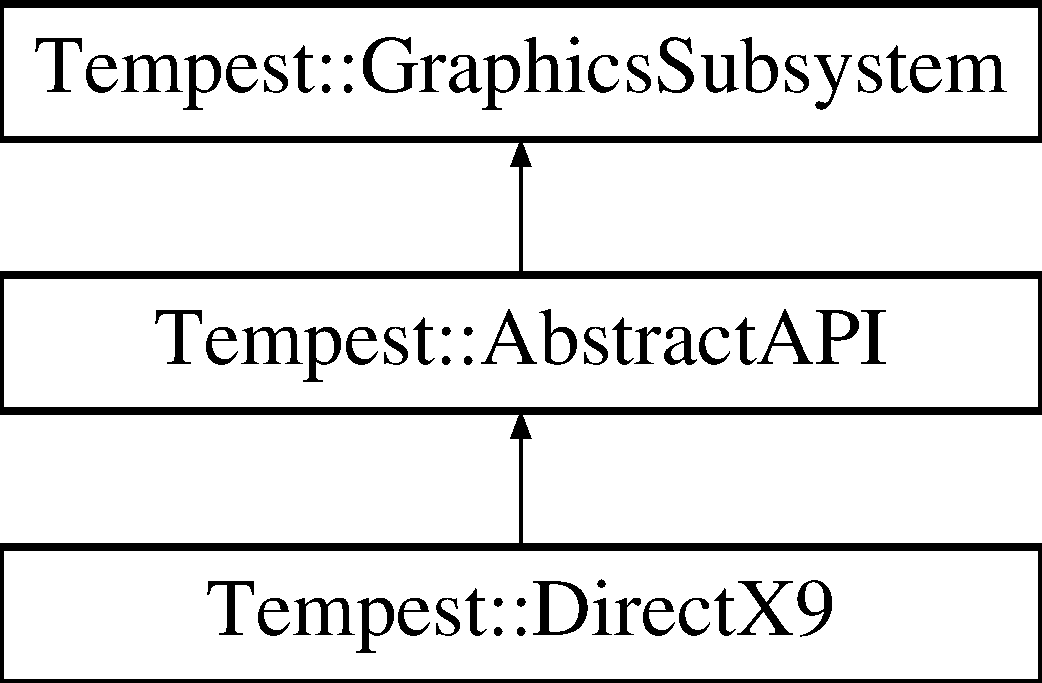
\includegraphics[height=3.000000cm]{class_tempest_1_1_direct_x9}
\end{center}
\end{figure}
\subsection*{Classes}
\begin{DoxyCompactItemize}
\item 
struct \hyperlink{struct_direct_x9_1_1_data}{Data}
\item 
struct \hyperlink{struct_direct_x9_1_1_device}{Device}
\item 
struct \hyperlink{struct_direct_x9_1_1_i_b_o}{I\+B\+O}
\end{DoxyCompactItemize}
\subsection*{Public Member Functions}
\begin{DoxyCompactItemize}
\item 
\hypertarget{class_tempest_1_1_direct_x9_a87c3952c033ae721e3c761fa0006a344}{\hyperlink{struct_tempest_1_1_abstract_a_p_i_1_1_caps}{Caps} {\bfseries caps} (\hyperlink{struct_direct_x9_1_1_device}{Device} $\ast$d) const }\label{class_tempest_1_1_direct_x9_a87c3952c033ae721e3c761fa0006a344}

\item 
\hypertarget{class_tempest_1_1_direct_x9_a3235c2e0ff1a33cdb169edebff4850b7}{std\+::string {\bfseries vendor} (Abstract\+A\+P\+I\+::\+Device $\ast$d) const }\label{class_tempest_1_1_direct_x9_a3235c2e0ff1a33cdb169edebff4850b7}

\item 
\hypertarget{class_tempest_1_1_direct_x9_ae1952bae2f62078ad8c4010d580b928f}{std\+::string {\bfseries renderer} (Abstract\+A\+P\+I\+::\+Device $\ast$d) const }\label{class_tempest_1_1_direct_x9_ae1952bae2f62078ad8c4010d580b928f}

\item 
\hypertarget{class_tempest_1_1_direct_x9_a3ff3562d2655ee049316aeaa9244baa2}{\hyperlink{struct_direct_x9_1_1_device}{Device} $\ast$ {\bfseries create\+Device} (void $\ast$hwnd, const \hyperlink{struct_tempest_1_1_abstract_a_p_i_1_1_options}{Options} \&opt) const }\label{class_tempest_1_1_direct_x9_a3ff3562d2655ee049316aeaa9244baa2}

\item 
\hypertarget{class_tempest_1_1_direct_x9_a629f78f9e0cedebb2d24a0446deb24bd}{void {\bfseries delete\+Device} (\hyperlink{struct_direct_x9_1_1_device}{Device} $\ast$d) const }\label{class_tempest_1_1_direct_x9_a629f78f9e0cedebb2d24a0446deb24bd}

\item 
\hypertarget{class_tempest_1_1_direct_x9_ada6c703e75fadcecda0a21d0da72075c}{void {\bfseries clear} (Abstract\+A\+P\+I\+::\+Device $\ast$d, const \hyperlink{class_tempest_1_1_color}{Color} \&cl, float z, unsigned stencil) const }\label{class_tempest_1_1_direct_x9_ada6c703e75fadcecda0a21d0da72075c}

\item 
\hypertarget{class_tempest_1_1_direct_x9_ad872bef43804a53e5bc41822cd1fc1d4}{void {\bfseries clear} (Abstract\+A\+P\+I\+::\+Device $\ast$d, const \hyperlink{class_tempest_1_1_color}{Color} \&cl) const }\label{class_tempest_1_1_direct_x9_ad872bef43804a53e5bc41822cd1fc1d4}

\item 
\hypertarget{class_tempest_1_1_direct_x9_a923f705de37c9743e43a4f6d0478df1c}{void {\bfseries clear} (Abstract\+A\+P\+I\+::\+Device $\ast$d, const \hyperlink{class_tempest_1_1_color}{Color} \&cl, float z) const }\label{class_tempest_1_1_direct_x9_a923f705de37c9743e43a4f6d0478df1c}

\item 
\hypertarget{class_tempest_1_1_direct_x9_a91314b6b0e5d4f1ebc6ef9c51165b48e}{void {\bfseries clear} (Abstract\+A\+P\+I\+::\+Device $\ast$d, float z, unsigned stencil) const }\label{class_tempest_1_1_direct_x9_a91314b6b0e5d4f1ebc6ef9c51165b48e}

\item 
\hypertarget{class_tempest_1_1_direct_x9_aa3bc0c3449f3576695fba69974a641cc}{void {\bfseries clear\+Z} (Abstract\+A\+P\+I\+::\+Device $\ast$d, float z) const }\label{class_tempest_1_1_direct_x9_aa3bc0c3449f3576695fba69974a641cc}

\item 
\hypertarget{class_tempest_1_1_direct_x9_af43614846b92a546f4e6ee57716163b3}{void {\bfseries clear\+Stencil} (Abstract\+A\+P\+I\+::\+Device $\ast$d, unsigned stencil) const }\label{class_tempest_1_1_direct_x9_af43614846b92a546f4e6ee57716163b3}

\item 
\hypertarget{class_tempest_1_1_direct_x9_a5257e82fe164fde620a00ad5be254efb}{void {\bfseries begin\+Paint} (Abstract\+A\+P\+I\+::\+Device $\ast$d) const }\label{class_tempest_1_1_direct_x9_a5257e82fe164fde620a00ad5be254efb}

\item 
\hypertarget{class_tempest_1_1_direct_x9_a7a378f4b41fc111fa08b3b21753fab97}{void {\bfseries end\+Paint} (Abstract\+A\+P\+I\+::\+Device $\ast$d) const }\label{class_tempest_1_1_direct_x9_a7a378f4b41fc111fa08b3b21753fab97}

\item 
\hypertarget{class_tempest_1_1_direct_x9_a662597640fa69fb0238e6b2f09a410a4}{void {\bfseries set\+Render\+State} (\hyperlink{struct_direct_x9_1_1_device}{Device} $\ast$d, const \hyperlink{class_tempest_1_1_render_state}{Render\+State} \&) const }\label{class_tempest_1_1_direct_x9_a662597640fa69fb0238e6b2f09a410a4}

\item 
\hypertarget{class_tempest_1_1_direct_x9_ac3fa20cc037ad1bb3cf32aa942348e6d}{void {\bfseries set\+Render\+Taget} (Abstract\+A\+P\+I\+::\+Device $\ast$d, Abstract\+A\+P\+I\+::\+Texture $\ast$tx, int mip, int mrt\+Slot) const }\label{class_tempest_1_1_direct_x9_ac3fa20cc037ad1bb3cf32aa942348e6d}

\item 
\hypertarget{class_tempest_1_1_direct_x9_a0de8c9bc2b57107919436b5ede1e86af}{void {\bfseries unset\+Render\+Tagets} (Abstract\+A\+P\+I\+::\+Device $\ast$d, int count) const }\label{class_tempest_1_1_direct_x9_a0de8c9bc2b57107919436b5ede1e86af}

\item 
\hypertarget{class_tempest_1_1_direct_x9_a22ad8d6d5d3a21ca2bfee5fac260140a}{void {\bfseries set\+D\+S\+Surface\+Taget} (Abstract\+A\+P\+I\+::\+Device $\ast$d, Std\+D\+S\+Surface $\ast$tx) const }\label{class_tempest_1_1_direct_x9_a22ad8d6d5d3a21ca2bfee5fac260140a}

\item 
\hypertarget{class_tempest_1_1_direct_x9_a66e60b211e993e9d5f811d0f33075670}{void {\bfseries set\+D\+S\+Surface\+Taget} (Abstract\+A\+P\+I\+::\+Device $\ast$d, Abstract\+A\+P\+I\+::\+Texture $\ast$tx) const }\label{class_tempest_1_1_direct_x9_a66e60b211e993e9d5f811d0f33075670}

\item 
\hypertarget{class_tempest_1_1_direct_x9_a2a15e9532b6a146569ddcc99e142b5ab}{Abstract\+A\+P\+I\+::\+Std\+D\+S\+Surface $\ast$ {\bfseries get\+D\+S\+Surface\+Taget} (Abstract\+A\+P\+I\+::\+Device $\ast$d) const }\label{class_tempest_1_1_direct_x9_a2a15e9532b6a146569ddcc99e142b5ab}

\item 
\hypertarget{class_tempest_1_1_direct_x9_ad3fe197c12fdc09ce025df3a066cb39b}{void {\bfseries ret\+D\+S\+Surface\+Taget} (Abstract\+A\+P\+I\+::\+Device $\ast$d, Abstract\+A\+P\+I\+::\+Std\+D\+S\+Surface $\ast$s) const }\label{class_tempest_1_1_direct_x9_ad3fe197c12fdc09ce025df3a066cb39b}

\item 
\hypertarget{class_tempest_1_1_direct_x9_af68144c80b9527f9f100ddf83dfcd8e4}{bool {\bfseries start\+Render} (Abstract\+A\+P\+I\+::\+Device $\ast$d, bool is\+Lost) const }\label{class_tempest_1_1_direct_x9_af68144c80b9527f9f100ddf83dfcd8e4}

\item 
\hypertarget{class_tempest_1_1_direct_x9_adf14e80a3109bdc2198a49b937778bec}{bool {\bfseries present} (Abstract\+A\+P\+I\+::\+Device $\ast$d, Swap\+Behavior b) const }\label{class_tempest_1_1_direct_x9_adf14e80a3109bdc2198a49b937778bec}

\item 
\hypertarget{class_tempest_1_1_direct_x9_aecdf7c4afd9287eb8ed1bbcf91453d7d}{bool {\bfseries reset} (Abstract\+A\+P\+I\+::\+Device $\ast$d, void $\ast$hwnd, const \hyperlink{struct_tempest_1_1_abstract_a_p_i_1_1_options}{Options} \&opt) const }\label{class_tempest_1_1_direct_x9_aecdf7c4afd9287eb8ed1bbcf91453d7d}

\item 
\hypertarget{class_tempest_1_1_direct_x9_a49045887af02ebb3a5aae52bd960beef}{bool {\bfseries is\+Format\+Supported} (Abstract\+A\+P\+I\+::\+Device $\ast$d, Pixmap\+::\+Format f) const }\label{class_tempest_1_1_direct_x9_a49045887af02ebb3a5aae52bd960beef}

\item 
\hypertarget{class_tempest_1_1_direct_x9_ad32422a654596592d2c5b8d63c15142a}{Abstract\+A\+P\+I\+::\+Texture $\ast$ {\bfseries create\+Texture} (Abstract\+A\+P\+I\+::\+Device $\ast$d, const std\+::string \&) const }\label{class_tempest_1_1_direct_x9_ad32422a654596592d2c5b8d63c15142a}

\item 
\hypertarget{class_tempest_1_1_direct_x9_a41ad54ef6d1f2ca4d9ef79247e65f254}{Abstract\+A\+P\+I\+::\+Texture $\ast$ {\bfseries create\+Texture} (Abstract\+A\+P\+I\+::\+Device $\ast$d, const \hyperlink{class_tempest_1_1_pixmap}{Pixmap} \&p, bool mips, bool compress) const }\label{class_tempest_1_1_direct_x9_a41ad54ef6d1f2ca4d9ef79247e65f254}

\item 
\hypertarget{class_tempest_1_1_direct_x9_a4bdf71403bd6227012136371a8c9be73}{Abstract\+A\+P\+I\+::\+Texture $\ast$ {\bfseries recreate\+Texture} (Abstract\+A\+P\+I\+::\+Device $\ast$d, const \hyperlink{class_tempest_1_1_pixmap}{Pixmap} \&p, bool mips, bool compress, Abstract\+A\+P\+I\+::\+Texture $\ast$t) const }\label{class_tempest_1_1_direct_x9_a4bdf71403bd6227012136371a8c9be73}

\item 
\hypertarget{class_tempest_1_1_direct_x9_a1267863a3f48d9013b3b20bdcd762813}{Abstract\+A\+P\+I\+::\+Texture $\ast$ {\bfseries create\+Texture} (Abstract\+A\+P\+I\+::\+Device $\ast$d, int w, int h, bool mips, \hyperlink{struct_tempest_1_1_abstract_texture_1_1_format_a231a1f516e53783bf72c713669b115b3}{Abstract\+Texture\+::\+Format\+::\+Type} f, Texture\+Usage usage) const }\label{class_tempest_1_1_direct_x9_a1267863a3f48d9013b3b20bdcd762813}

\item 
\hypertarget{class_tempest_1_1_direct_x9_aa971fa161847139b19e21fc0a06cffae}{Abstract\+A\+P\+I\+::\+Texture $\ast$ {\bfseries create\+Texture3d} (Abstract\+A\+P\+I\+::\+Device $\ast$d, int x, int y, int z, bool mips, \hyperlink{struct_tempest_1_1_abstract_texture_1_1_format_a231a1f516e53783bf72c713669b115b3}{Abstract\+Texture\+::\+Format\+::\+Type} f, Texture\+Usage usage, const char $\ast$data) const }\label{class_tempest_1_1_direct_x9_aa971fa161847139b19e21fc0a06cffae}

\item 
\hypertarget{class_tempest_1_1_direct_x9_aa71036e276637c1db1acb5f01595300e}{void {\bfseries generate\+Mipmaps} (Abstract\+A\+P\+I\+::\+Device $\ast$d, Abstract\+A\+P\+I\+::\+Texture $\ast$t) const }\label{class_tempest_1_1_direct_x9_aa71036e276637c1db1acb5f01595300e}

\item 
\hypertarget{class_tempest_1_1_direct_x9_a702be05b45834a30d673f88cded2da1f}{void {\bfseries delete\+Texture} (Abstract\+A\+P\+I\+::\+Device $\ast$d, Abstract\+A\+P\+I\+::\+Texture $\ast$t) const }\label{class_tempest_1_1_direct_x9_a702be05b45834a30d673f88cded2da1f}

\item 
\hypertarget{class_tempest_1_1_direct_x9_af8da297fcff932c9ecaa7a0163abc74d}{Abstract\+A\+P\+I\+::\+Vertex\+Buffer $\ast$ {\bfseries create\+Vertex\+Buffer} (Abstract\+A\+P\+I\+::\+Device $\ast$d, size\+\_\+t size, size\+\_\+t el\+Size, Buffer\+Usage u) const }\label{class_tempest_1_1_direct_x9_af8da297fcff932c9ecaa7a0163abc74d}

\item 
\hypertarget{class_tempest_1_1_direct_x9_a13ea63b17205313562967bea5c41c41b}{void {\bfseries delete\+Vertex\+Buffer} (Abstract\+A\+P\+I\+::\+Device $\ast$d, Abstract\+A\+P\+I\+::\+Vertex\+Buffer $\ast$) const }\label{class_tempest_1_1_direct_x9_a13ea63b17205313562967bea5c41c41b}

\item 
\hypertarget{class_tempest_1_1_direct_x9_a948f7173213bfa00ee8f535d9902bac6}{Abstract\+A\+P\+I\+::\+Index\+Buffer $\ast$ {\bfseries create\+Index\+Buffer} (Abstract\+A\+P\+I\+::\+Device $\ast$d, size\+\_\+t size, size\+\_\+t el\+Size, Buffer\+Usage u) const }\label{class_tempest_1_1_direct_x9_a948f7173213bfa00ee8f535d9902bac6}

\item 
\hypertarget{class_tempest_1_1_direct_x9_a64a062ad8b6cf9683302ff1671144ca1}{void {\bfseries delete\+Index\+Buffer} (Abstract\+A\+P\+I\+::\+Device $\ast$d, Abstract\+A\+P\+I\+::\+Index\+Buffer $\ast$) const }\label{class_tempest_1_1_direct_x9_a64a062ad8b6cf9683302ff1671144ca1}

\item 
\hypertarget{class_tempest_1_1_direct_x9_a8165b60f240a29a6638c847b58840526}{Abstract\+A\+P\+I\+::\+Vertex\+Decl $\ast$ {\bfseries create\+Vertex\+Decl} (Abstract\+A\+P\+I\+::\+Device $\ast$d, const \hyperlink{class_tempest_1_1_vertex_declaration_1_1_declarator}{Vertex\+Declaration\+::\+Declarator} \&de) const }\label{class_tempest_1_1_direct_x9_a8165b60f240a29a6638c847b58840526}

\item 
\hypertarget{class_tempest_1_1_direct_x9_a79009a974507370df1af9d9fca3fac47}{void {\bfseries delete\+Vertex\+Decl} (Abstract\+A\+P\+I\+::\+Device $\ast$d, Abstract\+A\+P\+I\+::\+Vertex\+Decl $\ast$) const }\label{class_tempest_1_1_direct_x9_a79009a974507370df1af9d9fca3fac47}

\item 
\hypertarget{class_tempest_1_1_direct_x9_aa20b7a4d0bfafe8c1378a6277effe7ac}{void {\bfseries set\+Vertex\+Declaration} (Abstract\+A\+P\+I\+::\+Device $\ast$d, Abstract\+A\+P\+I\+::\+Vertex\+Decl $\ast$) const }\label{class_tempest_1_1_direct_x9_aa20b7a4d0bfafe8c1378a6277effe7ac}

\item 
\hypertarget{class_tempest_1_1_direct_x9_a2ac117479f31e3cea42038145b9ca317}{void {\bfseries bind\+Vertex\+Buffer} (Abstract\+A\+P\+I\+::\+Device $\ast$d, Abstract\+A\+P\+I\+::\+Vertex\+Buffer $\ast$, int vsize) const }\label{class_tempest_1_1_direct_x9_a2ac117479f31e3cea42038145b9ca317}

\item 
\hypertarget{class_tempest_1_1_direct_x9_aa47203fe22b9e0d6223dc96644588704}{void {\bfseries bind\+Index\+Buffer} (Abstract\+A\+P\+I\+::\+Device $\ast$d, Abstract\+A\+P\+I\+::\+Index\+Buffer $\ast$) const }\label{class_tempest_1_1_direct_x9_aa47203fe22b9e0d6223dc96644588704}

\item 
\hypertarget{class_tempest_1_1_direct_x9_ac0a105d9a2dd57c36925d31e60264dd9}{void $\ast$ {\bfseries lock\+Buffer} (Abstract\+A\+P\+I\+::\+Device $\ast$d, Abstract\+A\+P\+I\+::\+Vertex\+Buffer $\ast$, unsigned offset, unsigned size) const }\label{class_tempest_1_1_direct_x9_ac0a105d9a2dd57c36925d31e60264dd9}

\item 
\hypertarget{class_tempest_1_1_direct_x9_a6ca1f32816c7c3210cd018de5257fb72}{void {\bfseries unlock\+Buffer} (Abstract\+A\+P\+I\+::\+Device $\ast$d, Abstract\+A\+P\+I\+::\+Vertex\+Buffer $\ast$) const }\label{class_tempest_1_1_direct_x9_a6ca1f32816c7c3210cd018de5257fb72}

\item 
\hypertarget{class_tempest_1_1_direct_x9_aa37bda6c3ea2a5d5c006efc7f5bd46ee}{void $\ast$ {\bfseries lock\+Buffer} (Abstract\+A\+P\+I\+::\+Device $\ast$d, Abstract\+A\+P\+I\+::\+Index\+Buffer $\ast$, unsigned offset, unsigned size) const }\label{class_tempest_1_1_direct_x9_aa37bda6c3ea2a5d5c006efc7f5bd46ee}

\item 
\hypertarget{class_tempest_1_1_direct_x9_a8508f22beed18b9297b119f06c0fc61a}{void {\bfseries unlock\+Buffer} (Abstract\+A\+P\+I\+::\+Device $\ast$d, Abstract\+A\+P\+I\+::\+Index\+Buffer $\ast$) const }\label{class_tempest_1_1_direct_x9_a8508f22beed18b9297b119f06c0fc61a}

\item 
\hypertarget{class_tempest_1_1_direct_x9_ac6ac8fae24e46b4a49ed52e26bc5178f}{\hyperlink{class_tempest_1_1_abstract_shading_lang}{Abstract\+Shading\+Lang} $\ast$ {\bfseries create\+Shading\+Lang} (Abstract\+A\+P\+I\+::\+Device $\ast$l) const }\label{class_tempest_1_1_direct_x9_ac6ac8fae24e46b4a49ed52e26bc5178f}

\item 
\hypertarget{class_tempest_1_1_direct_x9_aa45b2bc4954968c401c320e2fae59559}{void {\bfseries delete\+Shading\+Lang} (const \hyperlink{class_tempest_1_1_abstract_shading_lang}{Abstract\+Shading\+Lang} $\ast$l) const }\label{class_tempest_1_1_direct_x9_aa45b2bc4954968c401c320e2fae59559}

\item 
\hypertarget{class_tempest_1_1_direct_x9_a7db742148155ca628afdc0b8bf52f7db}{void {\bfseries draw} (Abstract\+A\+P\+I\+::\+Device $\ast$d, Abstract\+A\+P\+I\+::\+Primitive\+Type t, int first\+Vertex, int p\+Count) const }\label{class_tempest_1_1_direct_x9_a7db742148155ca628afdc0b8bf52f7db}

\item 
\hypertarget{class_tempest_1_1_direct_x9_a133bfc2af91d5c56e853054e5f63ab50}{void {\bfseries draw\+Indexed} (Abstract\+A\+P\+I\+::\+Device $\ast$d, Abstract\+A\+P\+I\+::\+Primitive\+Type t, int vbo\+Offset\+Index, int ibo\+Offset\+Index, int vertex\+Count) const }\label{class_tempest_1_1_direct_x9_a133bfc2af91d5c56e853054e5f63ab50}

\item 
\hypertarget{class_tempest_1_1_direct_x9_a0ca3f3eb56b614533a81800f21facf82}{\hyperlink{struct_tempest_1_1_size}{Size} {\bfseries window\+Size} (Tempest\+::\+Abstract\+A\+P\+I\+::\+Device $\ast$dev) const }\label{class_tempest_1_1_direct_x9_a0ca3f3eb56b614533a81800f21facf82}

\end{DoxyCompactItemize}
\subsection*{Additional Inherited Members}


The documentation for this class was generated from the following files\+:\begin{DoxyCompactItemize}
\item 
dx/directx9.\+h\item 
dx/directx9.\+cpp\end{DoxyCompactItemize}

\hypertarget{class_tempest_1_1_display_settings}{\section{Tempest\+:\+:Display\+Settings Class Reference}
\label{class_tempest_1_1_display_settings}\index{Tempest\+::\+Display\+Settings@{Tempest\+::\+Display\+Settings}}
}


screen display settings  




{\ttfamily \#include $<$displaysettings.\+h$>$}

\subsection*{Public Member Functions}
\begin{DoxyCompactItemize}
\item 
\hypertarget{class_tempest_1_1_display_settings_ae2695e8a3ef62e51ee14f763dc2a5da8}{{\bfseries Display\+Settings} (int w, int h, int bits=32, bool full\+Screen=false)}\label{class_tempest_1_1_display_settings_ae2695e8a3ef62e51ee14f763dc2a5da8}

\item 
\hypertarget{class_tempest_1_1_display_settings_af8bf6999fcbff3e9595c1e4e414664f8}{{\bfseries Display\+Settings} (const \hyperlink{struct_tempest_1_1_size}{Size} \&wh, int bits=32, bool full\+Screen=false)}\label{class_tempest_1_1_display_settings_af8bf6999fcbff3e9595c1e4e414664f8}

\item 
\hypertarget{class_tempest_1_1_display_settings_a1f7c227843fccdace05445f7406765ba}{\hyperlink{struct_tempest_1_1_size}{Size} {\bfseries size} () const }\label{class_tempest_1_1_display_settings_a1f7c227843fccdace05445f7406765ba}

\item 
\hypertarget{class_tempest_1_1_display_settings_a57d319c49348403338106bc26a741be2}{void {\bfseries set\+Size} (const \hyperlink{struct_tempest_1_1_size}{Size} \&s)}\label{class_tempest_1_1_display_settings_a57d319c49348403338106bc26a741be2}

\end{DoxyCompactItemize}
\subsection*{Public Attributes}
\begin{DoxyCompactItemize}
\item 
\hypertarget{class_tempest_1_1_display_settings_ac38b409a76cff6ac40baf6d819394ea3}{int {\bfseries width}}\label{class_tempest_1_1_display_settings_ac38b409a76cff6ac40baf6d819394ea3}

\item 
\hypertarget{class_tempest_1_1_display_settings_a341b61dc93be2ace7fbe1f3e9128af8b}{int {\bfseries height}}\label{class_tempest_1_1_display_settings_a341b61dc93be2ace7fbe1f3e9128af8b}

\item 
\hypertarget{class_tempest_1_1_display_settings_a6cb61a6265507aa912899bcdadd87820}{int {\bfseries bits}}\label{class_tempest_1_1_display_settings_a6cb61a6265507aa912899bcdadd87820}

\item 
\hypertarget{class_tempest_1_1_display_settings_a39a25d5c50c105d1b07bf37679960698}{bool {\bfseries full\+Screen}}\label{class_tempest_1_1_display_settings_a39a25d5c50c105d1b07bf37679960698}

\end{DoxyCompactItemize}


\subsection{Detailed Description}
screen display settings 

The documentation for this class was generated from the following files\+:\begin{DoxyCompactItemize}
\item 
core/wrappers/displaysettings.\+h\item 
core/wrappers/displaysettings.\+cpp\end{DoxyCompactItemize}

\hypertarget{class_tempest_1_1_drag_gesture}{\section{Tempest\+:\+:Drag\+Gesture Class Reference}
\label{class_tempest_1_1_drag_gesture}\index{Tempest\+::\+Drag\+Gesture@{Tempest\+::\+Drag\+Gesture}}
}
Inheritance diagram for Tempest\+:\+:Drag\+Gesture\+:\begin{figure}[H]
\begin{center}
\leavevmode
\includegraphics[height=3.000000cm]{class_tempest_1_1_drag_gesture}
\end{center}
\end{figure}
\subsection*{Public Member Functions}
\begin{DoxyCompactItemize}
\item 
\hypertarget{class_tempest_1_1_drag_gesture_aadf2d77a7fba3ee819183beed65603e5}{{\bfseries Drag\+Gesture} (\hyperlink{class_tempest_1_1_gesture_recognizer}{Gesture\+Recognizer} $\ast$owner, const \hyperlink{struct_tempest_1_1_point}{Point} \&s, const \hyperlink{struct_tempest_1_1_point}{Point} \&p, const \hyperlink{struct_tempest_1_1_point}{Point} \&d, State st)}\label{class_tempest_1_1_drag_gesture_aadf2d77a7fba3ee819183beed65603e5}

\end{DoxyCompactItemize}
\subsection*{Public Attributes}
\begin{DoxyCompactItemize}
\item 
\hypertarget{class_tempest_1_1_drag_gesture_a9b0f64e0760ea7fcaeba8b6feac3840a}{const \hyperlink{struct_tempest_1_1_point}{Point} {\bfseries start}}\label{class_tempest_1_1_drag_gesture_a9b0f64e0760ea7fcaeba8b6feac3840a}

\item 
\hypertarget{class_tempest_1_1_drag_gesture_a80b37f0d00981933a01de73a1fbd9a0d}{const \hyperlink{struct_tempest_1_1_point}{Point} {\bfseries pos}}\label{class_tempest_1_1_drag_gesture_a80b37f0d00981933a01de73a1fbd9a0d}

\item 
\hypertarget{class_tempest_1_1_drag_gesture_a0ca0612cd82374c3625f674c43090523}{const \hyperlink{struct_tempest_1_1_point}{Point} {\bfseries dpos}}\label{class_tempest_1_1_drag_gesture_a0ca0612cd82374c3625f674c43090523}

\end{DoxyCompactItemize}
\subsection*{Additional Inherited Members}


The documentation for this class was generated from the following file\+:\begin{DoxyCompactItemize}
\item 
ui/event.\+h\end{DoxyCompactItemize}

\hypertarget{struct_window_1_1_drag_gesture_recognizer}{\section{Tempest\+:\+:Window\+:\+:Drag\+Gesture\+Recognizer Struct Reference}
\label{struct_window_1_1_drag_gesture_recognizer}\index{Tempest\+::\+Window\+::\+Drag\+Gesture\+Recognizer@{Tempest\+::\+Window\+::\+Drag\+Gesture\+Recognizer}}
}
Inheritance diagram for Tempest\+:\+:Window\+:\+:Drag\+Gesture\+Recognizer\+:\begin{figure}[H]
\begin{center}
\leavevmode
\includegraphics[height=2.000000cm]{struct_window_1_1_drag_gesture_recognizer}
\end{center}
\end{figure}
\subsection*{Public Types}
\begin{DoxyCompactItemize}
\item 
\hypertarget{struct_window_1_1_drag_gesture_recognizer_af6ad3e83a79dea92e5a429b6ee64ae0a}{enum {\bfseries State} \{ {\bfseries Non\+Activated}, 
{\bfseries Press}, 
{\bfseries Move}
 \}}\label{struct_window_1_1_drag_gesture_recognizer_af6ad3e83a79dea92e5a429b6ee64ae0a}

\end{DoxyCompactItemize}
\subsection*{Public Member Functions}
\begin{DoxyCompactItemize}
\item 
\hypertarget{struct_window_1_1_drag_gesture_recognizer_a3463dc5ebbdda93c0d414d76b3e9fb97}{void {\bfseries delete\+Gesture} (\hyperlink{class_tempest_1_1_abstract_gesture_event}{Abstract\+Gesture\+Event} $\ast$g)}\label{struct_window_1_1_drag_gesture_recognizer_a3463dc5ebbdda93c0d414d76b3e9fb97}

\item 
\hypertarget{struct_window_1_1_drag_gesture_recognizer_aa2db7b37a81b7842f428e48bbaa20a3c}{\hyperlink{class_tempest_1_1_abstract_gesture_event}{Abstract\+Gesture\+Event} $\ast$ {\bfseries event} (const \hyperlink{class_tempest_1_1_event}{Event} \&e)}\label{struct_window_1_1_drag_gesture_recognizer_aa2db7b37a81b7842f428e48bbaa20a3c}

\end{DoxyCompactItemize}
\subsection*{Public Attributes}
\begin{DoxyCompactItemize}
\item 
\hypertarget{struct_window_1_1_drag_gesture_recognizer_a6857524ea5e940dacbb05e9e67e01496}{\hyperlink{class_tempest_1_1_mem_pool}{Mem\+Pool}$<$ \hyperlink{class_tempest_1_1_drag_gesture}{Drag\+Gesture} $>$ {\bfseries pool}}\label{struct_window_1_1_drag_gesture_recognizer_a6857524ea5e940dacbb05e9e67e01496}

\item 
\hypertarget{struct_window_1_1_drag_gesture_recognizer_ab6f37e7494d80666bb789de20ed856c8}{State {\bfseries state}}\label{struct_window_1_1_drag_gesture_recognizer_ab6f37e7494d80666bb789de20ed856c8}

\item 
\hypertarget{struct_window_1_1_drag_gesture_recognizer_ae8f6bcd31e26ba9916f14c070aac25a6}{int {\bfseries pointer}}\label{struct_window_1_1_drag_gesture_recognizer_ae8f6bcd31e26ba9916f14c070aac25a6}

\item 
\hypertarget{struct_window_1_1_drag_gesture_recognizer_af0f4931d90572a2fe30300d8fb785964}{\hyperlink{struct_tempest_1_1_point}{Point} {\bfseries spos}}\label{struct_window_1_1_drag_gesture_recognizer_af0f4931d90572a2fe30300d8fb785964}

\item 
\hypertarget{struct_window_1_1_drag_gesture_recognizer_acef11d15b3acead1730e0e038457c1ee}{\hyperlink{struct_tempest_1_1_point}{Point} {\bfseries pos}}\label{struct_window_1_1_drag_gesture_recognizer_acef11d15b3acead1730e0e038457c1ee}

\end{DoxyCompactItemize}


The documentation for this struct was generated from the following file\+:\begin{DoxyCompactItemize}
\item 
ui/window.\+cpp\end{DoxyCompactItemize}

\hypertarget{struct_tempest_1_1_opengl2x_1_1_device_1_1_dyn_buffer}{\section{Tempest\+:\+:Opengl2x\+:\+:Device\+:\+:Dyn\+Buffer Struct Reference}
\label{struct_tempest_1_1_opengl2x_1_1_device_1_1_dyn_buffer}\index{Tempest\+::\+Opengl2x\+::\+Device\+::\+Dyn\+Buffer@{Tempest\+::\+Opengl2x\+::\+Device\+::\+Dyn\+Buffer}}
}
\subsection*{Public Attributes}
\begin{DoxyCompactItemize}
\item 
\hypertarget{struct_tempest_1_1_opengl2x_1_1_device_1_1_dyn_buffer_a24509d20ab8b61f1318e0d8997f7acd9}{std\+::unordered\+\_\+set$<$ G\+Luint $>$ {\bfseries used}}\label{struct_tempest_1_1_opengl2x_1_1_device_1_1_dyn_buffer_a24509d20ab8b61f1318e0d8997f7acd9}

\item 
\hypertarget{struct_tempest_1_1_opengl2x_1_1_device_1_1_dyn_buffer_a5148cbdab27019480a8679baf8452927}{std\+::unordered\+\_\+set$<$ G\+Luint $>$ {\bfseries freed}}\label{struct_tempest_1_1_opengl2x_1_1_device_1_1_dyn_buffer_a5148cbdab27019480a8679baf8452927}

\end{DoxyCompactItemize}


The documentation for this struct was generated from the following file\+:\begin{DoxyCompactItemize}
\item 
ogl/opengl2x.\+cpp\end{DoxyCompactItemize}

\hypertarget{struct_texture_holder_1_1_data_1_1_dyn_texture}{\section{Tempest\+:\+:Texture\+Holder\+:\+:Data\+:\+:Dyn\+Texture Struct Reference}
\label{struct_texture_holder_1_1_data_1_1_dyn_texture}\index{Tempest\+::\+Texture\+Holder\+::\+Data\+::\+Dyn\+Texture@{Tempest\+::\+Texture\+Holder\+::\+Data\+::\+Dyn\+Texture}}
}
\subsection*{Public Attributes}
\begin{DoxyCompactItemize}
\item 
\hypertarget{struct_texture_holder_1_1_data_1_1_dyn_texture_aeb39e4e5f7a3979c3c151be06dc26841}{int {\bfseries w}}\label{struct_texture_holder_1_1_data_1_1_dyn_texture_aeb39e4e5f7a3979c3c151be06dc26841}

\item 
\hypertarget{struct_texture_holder_1_1_data_1_1_dyn_texture_a0e3ae67efcba86b99c7491ab23795ea4}{int {\bfseries h}}\label{struct_texture_holder_1_1_data_1_1_dyn_texture_a0e3ae67efcba86b99c7491ab23795ea4}

\item 
\hypertarget{struct_texture_holder_1_1_data_1_1_dyn_texture_a9691dc68de9e199343c07d316ca6138b}{int {\bfseries mip}}\label{struct_texture_holder_1_1_data_1_1_dyn_texture_a9691dc68de9e199343c07d316ca6138b}

\item 
\hypertarget{struct_texture_holder_1_1_data_1_1_dyn_texture_a23b34b352042dd38aeafcfcc732a2294}{Texture\+Usage {\bfseries usage}}\label{struct_texture_holder_1_1_data_1_1_dyn_texture_a23b34b352042dd38aeafcfcc732a2294}

\item 
\hypertarget{struct_texture_holder_1_1_data_1_1_dyn_texture_a542bf3f85322b413a3ec861dfbfdd4dd}{\hyperlink{struct_tempest_1_1_abstract_texture_1_1_format_a231a1f516e53783bf72c713669b115b3}{Abstract\+Texture\+::\+Format\+::\+Type} {\bfseries format}}\label{struct_texture_holder_1_1_data_1_1_dyn_texture_a542bf3f85322b413a3ec861dfbfdd4dd}

\item 
\hypertarget{struct_texture_holder_1_1_data_1_1_dyn_texture_ac7fb289a465cc6b2b558b62aca5d940c}{Abstract\+A\+P\+I\+::\+Texture $\ast$ {\bfseries owner}}\label{struct_texture_holder_1_1_data_1_1_dyn_texture_ac7fb289a465cc6b2b558b62aca5d940c}

\end{DoxyCompactItemize}


The documentation for this struct was generated from the following file\+:\begin{DoxyCompactItemize}
\item 
data\+Control/textureholder.\+cpp\end{DoxyCompactItemize}

\hypertarget{struct_volume_holder_1_1_data_1_1_dyn_texture}{\section{Tempest\+:\+:Volume\+Holder\+:\+:Data\+:\+:Dyn\+Texture Struct Reference}
\label{struct_volume_holder_1_1_data_1_1_dyn_texture}\index{Tempest\+::\+Volume\+Holder\+::\+Data\+::\+Dyn\+Texture@{Tempest\+::\+Volume\+Holder\+::\+Data\+::\+Dyn\+Texture}}
}
\subsection*{Public Attributes}
\begin{DoxyCompactItemize}
\item 
\hypertarget{struct_volume_holder_1_1_data_1_1_dyn_texture_a56a7a0c7eecf0be616a87ee89922357e}{int {\bfseries x}}\label{struct_volume_holder_1_1_data_1_1_dyn_texture_a56a7a0c7eecf0be616a87ee89922357e}

\item 
\hypertarget{struct_volume_holder_1_1_data_1_1_dyn_texture_af8683a8728cd5a724a7fe2c9d5220bc8}{int {\bfseries y}}\label{struct_volume_holder_1_1_data_1_1_dyn_texture_af8683a8728cd5a724a7fe2c9d5220bc8}

\item 
\hypertarget{struct_volume_holder_1_1_data_1_1_dyn_texture_a5ca86e588e35e43be0d2df88716da1b5}{int {\bfseries z}}\label{struct_volume_holder_1_1_data_1_1_dyn_texture_a5ca86e588e35e43be0d2df88716da1b5}

\item 
\hypertarget{struct_volume_holder_1_1_data_1_1_dyn_texture_aa4c3a7e51f95f9e81c1203758ed4793d}{int {\bfseries mip}}\label{struct_volume_holder_1_1_data_1_1_dyn_texture_aa4c3a7e51f95f9e81c1203758ed4793d}

\item 
\hypertarget{struct_volume_holder_1_1_data_1_1_dyn_texture_a98ecc7a7a1e306162882ef01a261a42e}{Texture\+Usage {\bfseries usage}}\label{struct_volume_holder_1_1_data_1_1_dyn_texture_a98ecc7a7a1e306162882ef01a261a42e}

\item 
\hypertarget{struct_volume_holder_1_1_data_1_1_dyn_texture_ad89b269d8abfa36170e25e959f05cff0}{\hyperlink{struct_tempest_1_1_abstract_texture_1_1_format_a231a1f516e53783bf72c713669b115b3}{Abstract\+Texture\+::\+Format\+::\+Type} {\bfseries format}}\label{struct_volume_holder_1_1_data_1_1_dyn_texture_ad89b269d8abfa36170e25e959f05cff0}

\end{DoxyCompactItemize}


The documentation for this struct was generated from the following file\+:\begin{DoxyCompactItemize}
\item 
data\+Control/volumeholder.\+cpp\end{DoxyCompactItemize}

\hypertarget{struct_tempest_1_1_vertex_declaration_1_1_declarator_1_1_element}{\section{Tempest\+:\+:Vertex\+Declaration\+:\+:Declarator\+:\+:Element Struct Reference}
\label{struct_tempest_1_1_vertex_declaration_1_1_declarator_1_1_element}\index{Tempest\+::\+Vertex\+Declaration\+::\+Declarator\+::\+Element@{Tempest\+::\+Vertex\+Declaration\+::\+Declarator\+::\+Element}}
}
\subsection*{Public Member Functions}
\begin{DoxyCompactItemize}
\item 
\hypertarget{struct_tempest_1_1_vertex_declaration_1_1_declarator_1_1_element_a877a619dbfc5d8d43a4d6dd33f597888}{bool {\bfseries operator==} (const \hyperlink{struct_tempest_1_1_vertex_declaration_1_1_declarator_1_1_element}{Element} \&d) const }\label{struct_tempest_1_1_vertex_declaration_1_1_declarator_1_1_element_a877a619dbfc5d8d43a4d6dd33f597888}

\item 
\hypertarget{struct_tempest_1_1_vertex_declaration_1_1_declarator_1_1_element_a90bc4d77caecbe7a8c64349097445aea}{bool {\bfseries operator!=} (const \hyperlink{struct_tempest_1_1_vertex_declaration_1_1_declarator_1_1_element}{Element} \&d) const }\label{struct_tempest_1_1_vertex_declaration_1_1_declarator_1_1_element_a90bc4d77caecbe7a8c64349097445aea}

\end{DoxyCompactItemize}
\subsection*{Public Attributes}
\begin{DoxyCompactItemize}
\item 
\hypertarget{struct_tempest_1_1_vertex_declaration_1_1_declarator_1_1_element_a7cf8e30c011cb58c0e58ca654412e280}{Tempest\+::\+Decl\+::\+Component\+Type {\bfseries component}}\label{struct_tempest_1_1_vertex_declaration_1_1_declarator_1_1_element_a7cf8e30c011cb58c0e58ca654412e280}

\item 
\hypertarget{struct_tempest_1_1_vertex_declaration_1_1_declarator_1_1_element_a0e8e63eab1065973ad122e72d26595a7}{Tempest\+::\+Usage\+::\+Usage\+Type {\bfseries usage}}\label{struct_tempest_1_1_vertex_declaration_1_1_declarator_1_1_element_a0e8e63eab1065973ad122e72d26595a7}

\item 
\hypertarget{struct_tempest_1_1_vertex_declaration_1_1_declarator_1_1_element_aee44040b7595d51091796e6d19453f43}{std\+::string {\bfseries attr\+Name}}\label{struct_tempest_1_1_vertex_declaration_1_1_declarator_1_1_element_aee44040b7595d51091796e6d19453f43}

\item 
\hypertarget{struct_tempest_1_1_vertex_declaration_1_1_declarator_1_1_element_ae8fba939dcd07b40257c6636f500a802}{int {\bfseries index}}\label{struct_tempest_1_1_vertex_declaration_1_1_declarator_1_1_element_ae8fba939dcd07b40257c6636f500a802}

\end{DoxyCompactItemize}


The documentation for this struct was generated from the following files\+:\begin{DoxyCompactItemize}
\item 
core/wrappers/vertexdeclaration.\+h\item 
core/wrappers/vertexdeclaration.\+cpp\end{DoxyCompactItemize}

\hypertarget{struct_tempest_1_1_e_t_c_codec}{\section{Tempest\+:\+:E\+T\+C\+Codec Struct Reference}
\label{struct_tempest_1_1_e_t_c_codec}\index{Tempest\+::\+E\+T\+C\+Codec@{Tempest\+::\+E\+T\+C\+Codec}}
}
Inheritance diagram for Tempest\+:\+:E\+T\+C\+Codec\+:\begin{figure}[H]
\begin{center}
\leavevmode
\includegraphics[height=2.000000cm]{struct_tempest_1_1_e_t_c_codec}
\end{center}
\end{figure}
\subsection*{Public Member Functions}
\begin{DoxyCompactItemize}
\item 
\hypertarget{struct_tempest_1_1_e_t_c_codec_a44cde5bcdf93148bcfddeadd57c4187d}{bool {\bfseries can\+Convert\+To} (const \hyperlink{struct_tempest_1_1_pixmap_1_1_img_info}{Img\+Info} \&info, Pixmap\+::\+Format fout) const }\label{struct_tempest_1_1_e_t_c_codec_a44cde5bcdf93148bcfddeadd57c4187d}

\item 
\hypertarget{struct_tempest_1_1_e_t_c_codec_a8ec533bdff969ff0afa49ea664403cf2}{bool {\bfseries can\+Save} (const \hyperlink{struct_tempest_1_1_pixmap_1_1_img_info}{Img\+Info} \&inf) const }\label{struct_tempest_1_1_e_t_c_codec_a8ec533bdff969ff0afa49ea664403cf2}

\item 
\hypertarget{struct_tempest_1_1_e_t_c_codec_a74adf3da0f09b8e9c2a74489f9f80eb4}{void {\bfseries compress\+Layer} (std\+::vector$<$ unsigned char $>$ \&img, std\+::vector$<$ unsigned char $>$ \&out, int w, int h)}\label{struct_tempest_1_1_e_t_c_codec_a74adf3da0f09b8e9c2a74489f9f80eb4}

\item 
\hypertarget{struct_tempest_1_1_e_t_c_codec_a788246dde3e239ba90bd2c4a4bcfcd87}{void {\bfseries from\+R\+G\+B} (\hyperlink{struct_tempest_1_1_pixmap_1_1_img_info}{Img\+Info} \&info, std\+::vector$<$ unsigned char $>$ \&img)}\label{struct_tempest_1_1_e_t_c_codec_a788246dde3e239ba90bd2c4a4bcfcd87}

\item 
\hypertarget{struct_tempest_1_1_e_t_c_codec_a991d41163b4d1ec924d02173831c7c21}{void {\bfseries to\+R\+G\+B} (\hyperlink{struct_tempest_1_1_pixmap_1_1_img_info}{Img\+Info} \&info, std\+::vector$<$ unsigned char $>$ \&inout, bool alpha)}\label{struct_tempest_1_1_e_t_c_codec_a991d41163b4d1ec924d02173831c7c21}

\item 
\hypertarget{struct_tempest_1_1_e_t_c_codec_a23984f355a74c55ccc1ab5ca16753a70}{bool {\bfseries save} (\hyperlink{class_tempest_1_1_o_device}{O\+Device} \&file, const \hyperlink{struct_tempest_1_1_pixmap_1_1_img_info}{Img\+Info} \&info, const std\+::vector$<$ unsigned char $>$ \&img)}\label{struct_tempest_1_1_e_t_c_codec_a23984f355a74c55ccc1ab5ca16753a70}

\item 
\hypertarget{struct_tempest_1_1_e_t_c_codec_a7d9e449546e9b48e9395e2c0486b97e8}{bool {\bfseries load} (\hyperlink{class_tempest_1_1_i_device}{I\+Device} \&data, \hyperlink{struct_tempest_1_1_pixmap_1_1_img_info}{Img\+Info} \&info, std\+::vector$<$ unsigned char $>$ \&out)}\label{struct_tempest_1_1_e_t_c_codec_a7d9e449546e9b48e9395e2c0486b97e8}

\end{DoxyCompactItemize}
\subsection*{Static Public Member Functions}
\begin{DoxyCompactItemize}
\item 
\hypertarget{struct_tempest_1_1_e_t_c_codec_a917c7da2294cc724f85ae2d82170feb0}{static bool {\bfseries etc\+Frm} (Pixmap\+::\+Format fout)}\label{struct_tempest_1_1_e_t_c_codec_a917c7da2294cc724f85ae2d82170feb0}

\end{DoxyCompactItemize}
\subsection*{Additional Inherited Members}


The documentation for this struct was generated from the following file\+:\begin{DoxyCompactItemize}
\item 
core/imagecodec.\+cpp\end{DoxyCompactItemize}

\hypertarget{struct_tempest_1_1_graphics_subsystem_1_1_event}{\section{Tempest\+:\+:Graphics\+Subsystem\+:\+:Event Struct Reference}
\label{struct_tempest_1_1_graphics_subsystem_1_1_event}\index{Tempest\+::\+Graphics\+Subsystem\+::\+Event@{Tempest\+::\+Graphics\+Subsystem\+::\+Event}}
}
Inheritance diagram for Tempest\+:\+:Graphics\+Subsystem\+:\+:Event\+:\begin{figure}[H]
\begin{center}
\leavevmode
\includegraphics[height=2.000000cm]{struct_tempest_1_1_graphics_subsystem_1_1_event}
\end{center}
\end{figure}
\subsection*{Public Types}
\begin{DoxyCompactItemize}
\item 
\hypertarget{struct_tempest_1_1_graphics_subsystem_1_1_event_aee9c81a4df7bf24670fbec79fc13054d}{enum {\bfseries Type} \{ {\bfseries No\+Event}, 
{\bfseries Delete\+Object}, 
{\bfseries Count}
 \}}\label{struct_tempest_1_1_graphics_subsystem_1_1_event_aee9c81a4df7bf24670fbec79fc13054d}

\end{DoxyCompactItemize}
\subsection*{Public Attributes}
\begin{DoxyCompactItemize}
\item 
\hypertarget{struct_tempest_1_1_graphics_subsystem_1_1_event_a6f95f8855a6d2008b6988aa941ecee20}{Type {\bfseries type}}\label{struct_tempest_1_1_graphics_subsystem_1_1_event_a6f95f8855a6d2008b6988aa941ecee20}

\end{DoxyCompactItemize}


The documentation for this struct was generated from the following files\+:\begin{DoxyCompactItemize}
\item 
core/graphicssubsystem.\+h\item 
core/graphicssubsystem.\+cpp\end{DoxyCompactItemize}

\hypertarget{class_tempest_1_1_event}{\section{Tempest\+:\+:Event Class Reference}
\label{class_tempest_1_1_event}\index{Tempest\+::\+Event@{Tempest\+::\+Event}}
}


abstract event class  




{\ttfamily \#include $<$event.\+h$>$}

Inheritance diagram for Tempest\+:\+:Event\+:\begin{figure}[H]
\begin{center}
\leavevmode
\includegraphics[height=1.230769cm]{class_tempest_1_1_event}
\end{center}
\end{figure}
\subsection*{Public Types}
\begin{DoxyCompactItemize}
\item 
\hypertarget{class_tempest_1_1_event_abaea3e734410b7e9364cf2c75edf60b0}{enum {\bfseries Type} \{ \\*
{\bfseries No\+Event} = 0, 
{\bfseries Mouse\+Down}, 
{\bfseries Mouse\+Up}, 
{\bfseries Mouse\+Move}, 
\\*
{\bfseries Mouse\+Drag}, 
{\bfseries Mouse\+Wheel}, 
{\bfseries Key\+Down}, 
{\bfseries Key\+Up}, 
\\*
{\bfseries Resize}, 
{\bfseries Shortcut}, 
{\bfseries Paint}, 
{\bfseries Close}, 
\\*
{\bfseries Gesture}, 
{\bfseries Custom} = 512
 \}}\label{class_tempest_1_1_event_abaea3e734410b7e9364cf2c75edf60b0}

\item 
\hypertarget{class_tempest_1_1_event_a06f9d48d16768b58b74b1fbf83590aa8}{enum {\bfseries Mouse\+Button} \{ {\bfseries Button\+None} = 0, 
{\bfseries Button\+Left}, 
{\bfseries Button\+Right}, 
{\bfseries Button\+Mid}
 \}}\label{class_tempest_1_1_event_a06f9d48d16768b58b74b1fbf83590aa8}

\item 
\hypertarget{class_tempest_1_1_event_a5c66a7404768986697634059fef5cd93}{enum {\bfseries Key\+Type} \{ \\*
{\bfseries K\+\_\+\+No\+Key} = 0, 
{\bfseries K\+\_\+\+E\+S\+C\+A\+P\+E}, 
{\bfseries K\+\_\+\+Left}, 
{\bfseries K\+\_\+\+Up}, 
\\*
{\bfseries K\+\_\+\+Right}, 
{\bfseries K\+\_\+\+Down}, 
{\bfseries K\+\_\+\+Back}, 
{\bfseries K\+\_\+\+Delete}, 
\\*
{\bfseries K\+\_\+\+Insert}, 
{\bfseries K\+\_\+\+Return}, 
{\bfseries K\+\_\+\+Home}, 
{\bfseries K\+\_\+\+End}, 
\\*
{\bfseries K\+\_\+\+Pause}, 
{\bfseries K\+\_\+\+F1}, 
{\bfseries K\+\_\+\+F2}, 
{\bfseries K\+\_\+\+F3}, 
\\*
{\bfseries K\+\_\+\+F4}, 
{\bfseries K\+\_\+\+F5}, 
{\bfseries K\+\_\+\+F6}, 
{\bfseries K\+\_\+\+F7}, 
\\*
{\bfseries K\+\_\+\+F8}, 
{\bfseries K\+\_\+\+F9}, 
{\bfseries K\+\_\+\+F10}, 
{\bfseries K\+\_\+\+F11}, 
\\*
{\bfseries K\+\_\+\+F12}, 
{\bfseries K\+\_\+\+F13}, 
{\bfseries K\+\_\+\+F14}, 
{\bfseries K\+\_\+\+F15}, 
\\*
{\bfseries K\+\_\+\+F16}, 
{\bfseries K\+\_\+\+F17}, 
{\bfseries K\+\_\+\+F18}, 
{\bfseries K\+\_\+\+F19}, 
\\*
{\bfseries K\+\_\+\+F20}, 
{\bfseries K\+\_\+\+F21}, 
{\bfseries K\+\_\+\+F22}, 
{\bfseries K\+\_\+\+F23}, 
\\*
{\bfseries K\+\_\+\+F24}, 
{\bfseries K\+\_\+\+A}, 
{\bfseries K\+\_\+\+B}, 
{\bfseries K\+\_\+\+C}, 
\\*
{\bfseries K\+\_\+\+D}, 
{\bfseries K\+\_\+\+E}, 
{\bfseries K\+\_\+\+F}, 
{\bfseries K\+\_\+\+G}, 
\\*
{\bfseries K\+\_\+\+H}, 
{\bfseries K\+\_\+\+I}, 
{\bfseries K\+\_\+\+J}, 
{\bfseries K\+\_\+\+K}, 
\\*
{\bfseries K\+\_\+\+L}, 
{\bfseries K\+\_\+\+M}, 
{\bfseries K\+\_\+\+N}, 
{\bfseries K\+\_\+\+O}, 
\\*
{\bfseries K\+\_\+\+P}, 
{\bfseries K\+\_\+\+Q}, 
{\bfseries K\+\_\+\+R}, 
{\bfseries K\+\_\+\+S}, 
\\*
{\bfseries K\+\_\+\+T}, 
{\bfseries K\+\_\+\+U}, 
{\bfseries K\+\_\+\+V}, 
{\bfseries K\+\_\+\+W}, 
\\*
{\bfseries K\+\_\+\+X}, 
{\bfseries K\+\_\+\+Y}, 
{\bfseries K\+\_\+\+Z}, 
{\bfseries K\+\_\+0}, 
\\*
{\bfseries K\+\_\+1}, 
{\bfseries K\+\_\+2}, 
{\bfseries K\+\_\+3}, 
{\bfseries K\+\_\+4}, 
\\*
{\bfseries K\+\_\+5}, 
{\bfseries K\+\_\+6}, 
{\bfseries K\+\_\+7}, 
{\bfseries K\+\_\+8}, 
\\*
{\bfseries K\+\_\+9}, 
{\bfseries K\+\_\+\+Last}
 \}}\label{class_tempest_1_1_event_a5c66a7404768986697634059fef5cd93}

\end{DoxyCompactItemize}
\subsection*{Public Member Functions}
\begin{DoxyCompactItemize}
\item 
\hypertarget{class_tempest_1_1_event_a09af39b1579c9c2f4af900106e16b28f}{void {\bfseries accept} ()}\label{class_tempest_1_1_event_a09af39b1579c9c2f4af900106e16b28f}

\item 
\hypertarget{class_tempest_1_1_event_ab48b274894b28736e245334629d0c41a}{void {\bfseries ignore} ()}\label{class_tempest_1_1_event_ab48b274894b28736e245334629d0c41a}

\item 
\hypertarget{class_tempest_1_1_event_afc59a38e9e55fc3fa55931fa87dee87e}{bool {\bfseries is\+Accepted} () const }\label{class_tempest_1_1_event_afc59a38e9e55fc3fa55931fa87dee87e}

\item 
\hypertarget{class_tempest_1_1_event_a6797a844bda6e7da41403410eafaaa8b}{Type {\bfseries type} () const }\label{class_tempest_1_1_event_a6797a844bda6e7da41403410eafaaa8b}

\end{DoxyCompactItemize}
\subsection*{Protected Member Functions}
\begin{DoxyCompactItemize}
\item 
\hypertarget{class_tempest_1_1_event_ad949aed40780cdfb855457a1a8753d3e}{void {\bfseries set\+Type} (Type t)}\label{class_tempest_1_1_event_ad949aed40780cdfb855457a1a8753d3e}

\end{DoxyCompactItemize}
\subsection*{Friends}
\begin{DoxyCompactItemize}
\item 
\hypertarget{class_tempest_1_1_event_a81a96e8e06bdd16bd87b9bff53d8f1d7}{class {\bfseries System\+A\+P\+I}}\label{class_tempest_1_1_event_a81a96e8e06bdd16bd87b9bff53d8f1d7}

\end{DoxyCompactItemize}


\subsection{Detailed Description}
abstract event class 

The documentation for this class was generated from the following files\+:\begin{DoxyCompactItemize}
\item 
ui/event.\+h\item 
ui/event.\+cpp\end{DoxyCompactItemize}

\hypertarget{struct_tempest_1_1_opengl2x_1_1_device_1_1_f_b_os}{\section{Tempest\+:\+:Opengl2x\+:\+:Device\+:\+:F\+B\+Os Struct Reference}
\label{struct_tempest_1_1_opengl2x_1_1_device_1_1_f_b_os}\index{Tempest\+::\+Opengl2x\+::\+Device\+::\+F\+B\+Os@{Tempest\+::\+Opengl2x\+::\+Device\+::\+F\+B\+Os}}
}
\subsection*{Classes}
\begin{DoxyCompactItemize}
\item 
struct \hyperlink{struct_tempest_1_1_opengl2x_1_1_device_1_1_f_b_os_1_1_bucket}{Bucket}
\end{DoxyCompactItemize}
\subsection*{Public Member Functions}
\begin{DoxyCompactItemize}
\item 
\hypertarget{struct_tempest_1_1_opengl2x_1_1_device_1_1_f_b_os_a8832819ef5c4c42360de90cef82bb9c4}{void {\bfseries on\+Delete\+Texture} (Detail\+::\+G\+L\+Texture $\ast$t)}\label{struct_tempest_1_1_opengl2x_1_1_device_1_1_f_b_os_a8832819ef5c4c42360de90cef82bb9c4}

\item 
\hypertarget{struct_tempest_1_1_opengl2x_1_1_device_1_1_f_b_os_a97f57cfd78d6b94135f138e343ca9727}{void {\bfseries on\+Delete\+Texture} (\hyperlink{struct_tempest_1_1_opengl2x_1_1_device_1_1_f_b_os_1_1_bucket}{Bucket} \&b, Detail\+::\+G\+L\+Texture $\ast$t)}\label{struct_tempest_1_1_opengl2x_1_1_device_1_1_f_b_os_a97f57cfd78d6b94135f138e343ca9727}

\item 
\hypertarget{struct_tempest_1_1_opengl2x_1_1_device_1_1_f_b_os_a418f24c79cecb60aaebd66a1c75d0642}{bool {\bfseries cmp\+Tagets} (const Detail\+::\+Render\+Tg \&tg, Detail\+::\+G\+L\+Texture $\ast$$\ast$rtg, int $\ast$mip, int sz)}\label{struct_tempest_1_1_opengl2x_1_1_device_1_1_f_b_os_a418f24c79cecb60aaebd66a1c75d0642}

\item 
\hypertarget{struct_tempest_1_1_opengl2x_1_1_device_1_1_f_b_os_ae97727dcb94e0659f0056291ee0aa3ce}{G\+Luint \& {\bfseries get\+Target} (const Detail\+::\+Render\+Tg \&tg, int sz, size\+\_\+t \&hash)}\label{struct_tempest_1_1_opengl2x_1_1_device_1_1_f_b_os_ae97727dcb94e0659f0056291ee0aa3ce}

\item 
\hypertarget{struct_tempest_1_1_opengl2x_1_1_device_1_1_f_b_os_ac8aea39ba3cb4d7af7c0c2008548da7d}{\hyperlink{struct_tempest_1_1_opengl2x_1_1_device_1_1_f_b_os_1_1_bucket}{Bucket} \& {\bfseries bucket} (int mrt)}\label{struct_tempest_1_1_opengl2x_1_1_device_1_1_f_b_os_ac8aea39ba3cb4d7af7c0c2008548da7d}

\end{DoxyCompactItemize}
\subsection*{Public Attributes}
\begin{DoxyCompactItemize}
\item 
\hypertarget{struct_tempest_1_1_opengl2x_1_1_device_1_1_f_b_os_a40761b3d51c374c2447596b93cedaefb}{std\+::vector$<$ \hyperlink{struct_tempest_1_1_opengl2x_1_1_device_1_1_f_b_os_1_1_bucket}{Bucket} $>$ {\bfseries buckets}}\label{struct_tempest_1_1_opengl2x_1_1_device_1_1_f_b_os_a40761b3d51c374c2447596b93cedaefb}

\end{DoxyCompactItemize}


The documentation for this struct was generated from the following file\+:\begin{DoxyCompactItemize}
\item 
ogl/opengl2x.\+cpp\end{DoxyCompactItemize}

\hypertarget{struct_tempest_1_1_abstract_texture_1_1_filter_type}{\section{Tempest\+:\+:Abstract\+Texture\+:\+:Filter\+Type Struct Reference}
\label{struct_tempest_1_1_abstract_texture_1_1_filter_type}\index{Tempest\+::\+Abstract\+Texture\+::\+Filter\+Type@{Tempest\+::\+Abstract\+Texture\+::\+Filter\+Type}}
}


Способы фильтрации текстуры.  




{\ttfamily \#include $<$abstracttexture.\+h$>$}

\subsection*{Public Types}
\begin{DoxyCompactItemize}
\item 
enum \hyperlink{struct_tempest_1_1_abstract_texture_1_1_filter_type_aa28dcbdc63244fe43cfb7258f6996978}{Type} \{ \hyperlink{struct_tempest_1_1_abstract_texture_1_1_filter_type_aa28dcbdc63244fe43cfb7258f6996978a484d5ec433c09e3e650a5edbb354df06}{Nearest}, 
\hyperlink{struct_tempest_1_1_abstract_texture_1_1_filter_type_aa28dcbdc63244fe43cfb7258f6996978a045ff1a08bf815cbf4a46e9da4a8c506}{Linear}, 
\hyperlink{struct_tempest_1_1_abstract_texture_1_1_filter_type_aa28dcbdc63244fe43cfb7258f6996978a9d8f7121f7130f9bc78c4017e8c6962f}{Count}
 \}
\begin{DoxyCompactList}\small\item\em Способы фильтрации текстуры. \end{DoxyCompactList}\end{DoxyCompactItemize}


\subsection{Detailed Description}
Способы фильтрации текстуры. 

\subsection{Member Enumeration Documentation}
\hypertarget{struct_tempest_1_1_abstract_texture_1_1_filter_type_aa28dcbdc63244fe43cfb7258f6996978}{\index{Tempest\+::\+Abstract\+Texture\+::\+Filter\+Type@{Tempest\+::\+Abstract\+Texture\+::\+Filter\+Type}!Type@{Type}}
\index{Type@{Type}!Tempest\+::\+Abstract\+Texture\+::\+Filter\+Type@{Tempest\+::\+Abstract\+Texture\+::\+Filter\+Type}}
\subsubsection[{Type}]{\setlength{\rightskip}{0pt plus 5cm}enum {\bf Tempest\+::\+Abstract\+Texture\+::\+Filter\+Type\+::\+Type}}}\label{struct_tempest_1_1_abstract_texture_1_1_filter_type_aa28dcbdc63244fe43cfb7258f6996978}


Способы фильтрации текстуры. 

\begin{Desc}
\item[Enumerator]\par
\begin{description}
\index{Nearest@{Nearest}!Tempest\+::\+Abstract\+Texture\+::\+Filter\+Type@{Tempest\+::\+Abstract\+Texture\+::\+Filter\+Type}}\index{Tempest\+::\+Abstract\+Texture\+::\+Filter\+Type@{Tempest\+::\+Abstract\+Texture\+::\+Filter\+Type}!Nearest@{Nearest}}\item[{\em 
\hypertarget{struct_tempest_1_1_abstract_texture_1_1_filter_type_aa28dcbdc63244fe43cfb7258f6996978a484d5ec433c09e3e650a5edbb354df06}{Nearest}\label{struct_tempest_1_1_abstract_texture_1_1_filter_type_aa28dcbdc63244fe43cfb7258f6996978a484d5ec433c09e3e650a5edbb354df06}
}]ближайшая фильтрация \index{Linear@{Linear}!Tempest\+::\+Abstract\+Texture\+::\+Filter\+Type@{Tempest\+::\+Abstract\+Texture\+::\+Filter\+Type}}\index{Tempest\+::\+Abstract\+Texture\+::\+Filter\+Type@{Tempest\+::\+Abstract\+Texture\+::\+Filter\+Type}!Linear@{Linear}}\item[{\em 
\hypertarget{struct_tempest_1_1_abstract_texture_1_1_filter_type_aa28dcbdc63244fe43cfb7258f6996978a045ff1a08bf815cbf4a46e9da4a8c506}{Linear}\label{struct_tempest_1_1_abstract_texture_1_1_filter_type_aa28dcbdc63244fe43cfb7258f6996978a045ff1a08bf815cbf4a46e9da4a8c506}
}]линейная фильтрация \index{Count@{Count}!Tempest\+::\+Abstract\+Texture\+::\+Filter\+Type@{Tempest\+::\+Abstract\+Texture\+::\+Filter\+Type}}\index{Tempest\+::\+Abstract\+Texture\+::\+Filter\+Type@{Tempest\+::\+Abstract\+Texture\+::\+Filter\+Type}!Count@{Count}}\item[{\em 
\hypertarget{struct_tempest_1_1_abstract_texture_1_1_filter_type_aa28dcbdc63244fe43cfb7258f6996978a9d8f7121f7130f9bc78c4017e8c6962f}{Count}\label{struct_tempest_1_1_abstract_texture_1_1_filter_type_aa28dcbdc63244fe43cfb7258f6996978a9d8f7121f7130f9bc78c4017e8c6962f}
}]Count. \end{description}
\end{Desc}


The documentation for this struct was generated from the following file\+:\begin{DoxyCompactItemize}
\item 
core/wrappers/abstracttexture.\+h\end{DoxyCompactItemize}

\hypertarget{class_tempest_1_1_font}{\section{Tempest\+:\+:Font Class Reference}
\label{class_tempest_1_1_font}\index{Tempest\+::\+Font@{Tempest\+::\+Font}}
}
\subsection*{Public Types}
\begin{DoxyCompactItemize}
\item 
\hypertarget{class_tempest_1_1_font_ab637228c56251c80f84f3439fcc46ad8}{typedef \hyperlink{struct_tempest_1_1_font_element_1_1_letter_geometry}{Font\+Element\+::\+Letter\+Geometry} {\bfseries Letter\+Geometry}}\label{class_tempest_1_1_font_ab637228c56251c80f84f3439fcc46ad8}

\item 
\hypertarget{class_tempest_1_1_font_aa5d7206380af0fbfbad2066f38dcce8d}{typedef \hyperlink{struct_tempest_1_1_font_element_1_1_letter}{Font\+Element\+::\+Letter} {\bfseries Letter}}\label{class_tempest_1_1_font_aa5d7206380af0fbfbad2066f38dcce8d}

\end{DoxyCompactItemize}
\subsection*{Public Member Functions}
\begin{DoxyCompactItemize}
\item 
\hypertarget{class_tempest_1_1_font_aa47cbc7fe16d66523df3d4b61259b20e}{{\bfseries Font} (const std\+::string \&name, int sz)}\label{class_tempest_1_1_font_aa47cbc7fe16d66523df3d4b61259b20e}

\item 
\hypertarget{class_tempest_1_1_font_a99661caf6c603f938b11cd0514c4bab3}{{\bfseries Font} (const \hyperlink{class_tempest_1_1_font_element}{Font\+Element} \&n, const \hyperlink{class_tempest_1_1_font_element}{Font\+Element} \&b, const \hyperlink{class_tempest_1_1_font_element}{Font\+Element} \&i, const \hyperlink{class_tempest_1_1_font_element}{Font\+Element} \&bi)}\label{class_tempest_1_1_font_a99661caf6c603f938b11cd0514c4bab3}

\item 
\hypertarget{class_tempest_1_1_font_ac8050327320b0764b39b23e6f7de9211}{int {\bfseries size} () const }\label{class_tempest_1_1_font_ac8050327320b0764b39b23e6f7de9211}

\item 
\hypertarget{class_tempest_1_1_font_a109b219af47717db100f53707e881716}{void {\bfseries set\+Size} (int s)}\label{class_tempest_1_1_font_a109b219af47717db100f53707e881716}

\item 
\hypertarget{class_tempest_1_1_font_a531bd724c393fa176012a27319a33d2c}{void {\bfseries set\+Bold} (bool b)}\label{class_tempest_1_1_font_a531bd724c393fa176012a27319a33d2c}

\item 
\hypertarget{class_tempest_1_1_font_a18807ac4987e8dc12970be679d05f51e}{bool {\bfseries is\+Bold} () const }\label{class_tempest_1_1_font_a18807ac4987e8dc12970be679d05f51e}

\item 
\hypertarget{class_tempest_1_1_font_a5949fac71a2996e307cf06ed1f22ea5a}{void {\bfseries set\+Italic} (bool b)}\label{class_tempest_1_1_font_a5949fac71a2996e307cf06ed1f22ea5a}

\item 
\hypertarget{class_tempest_1_1_font_a81ba6828da30e452ce937d613a6ec991}{bool {\bfseries is\+Italic} () const }\label{class_tempest_1_1_font_a81ba6828da30e452ce937d613a6ec991}

\item 
\hypertarget{class_tempest_1_1_font_a6ec302204706267e8984cb9715a85427}{void {\bfseries fetch} (const std\+::u16string \&str, \hyperlink{class_tempest_1_1_sprites_holder}{Sprites\+Holder} \&sp) const }\label{class_tempest_1_1_font_a6ec302204706267e8984cb9715a85427}

\item 
\hypertarget{class_tempest_1_1_font_afc66f42b1ee2ea266da838ce6d1ec93e}{void {\bfseries fetch} (const std\+::string \&str, \hyperlink{class_tempest_1_1_sprites_holder}{Sprites\+Holder} \&sp) const }\label{class_tempest_1_1_font_afc66f42b1ee2ea266da838ce6d1ec93e}

\item 
\hypertarget{class_tempest_1_1_font_afd325296e8bfa69a11004ddce21a3317}{const \hyperlink{struct_tempest_1_1_font_element_1_1_letter}{Letter} \& {\bfseries letter} (char16\+\_\+t ch, \hyperlink{class_tempest_1_1_sprites_holder}{Sprites\+Holder} \&sp) const }\label{class_tempest_1_1_font_afd325296e8bfa69a11004ddce21a3317}

\item 
\hypertarget{class_tempest_1_1_font_af2ba7bbc0fa44d5ff458f92853ed5d77}{\hyperlink{struct_tempest_1_1_font_element_1_1_letter_geometry}{Letter\+Geometry} {\bfseries letter\+Geometry} (char16\+\_\+t ch) const }\label{class_tempest_1_1_font_af2ba7bbc0fa44d5ff458f92853ed5d77}

\item 
\hypertarget{class_tempest_1_1_font_a8a18f6ceacad37ddfb418d2d9a7dbe76}{\hyperlink{struct_tempest_1_1_size}{Size} {\bfseries text\+Size} (const std\+::u16string \&)}\label{class_tempest_1_1_font_a8a18f6ceacad37ddfb418d2d9a7dbe76}

\item 
\hypertarget{class_tempest_1_1_font_ac7543ca4e64d5aee3f02679709b4ac1c}{\hyperlink{struct_tempest_1_1_size}{Size} {\bfseries text\+Size} (const std\+::string \&)}\label{class_tempest_1_1_font_ac7543ca4e64d5aee3f02679709b4ac1c}

\item 
\hypertarget{class_tempest_1_1_font_aed3861c4b014e7e2a0f2738adf2f0cc5}{\hyperlink{struct_tempest_1_1_size}{Size} {\bfseries text\+Size} (const char16\+\_\+t $\ast$b, const char16\+\_\+t $\ast$e)}\label{class_tempest_1_1_font_aed3861c4b014e7e2a0f2738adf2f0cc5}

\item 
\hypertarget{class_tempest_1_1_font_a5aa8845660752a9c9c9af54a62e5101e}{\hyperlink{struct_tempest_1_1_size}{Size} {\bfseries text\+Size} (const char $\ast$b, const char $\ast$e)}\label{class_tempest_1_1_font_a5aa8845660752a9c9c9af54a62e5101e}

\item 
\hypertarget{class_tempest_1_1_font_a07ce8d1efa336475332069babce6df2f}{\hyperlink{struct_tempest_1_1_size}{Size} {\bfseries text\+Size} (const char16\+\_\+t $\ast$str)}\label{class_tempest_1_1_font_a07ce8d1efa336475332069babce6df2f}

\item 
\hypertarget{class_tempest_1_1_font_aa29edd6a150c5862797313b76a26a5f5}{\hyperlink{struct_tempest_1_1_size}{Size} {\bfseries text\+Size} (const char $\ast$str)}\label{class_tempest_1_1_font_aa29edd6a150c5862797313b76a26a5f5}

\end{DoxyCompactItemize}


\subsection{Detailed Description}
\begin{Desc}
\item[Examples\+: ]\par
\hyperlink{_painting2d_2mainwindow_8cpp-example}{Painting2d/mainwindow.\+cpp}.\end{Desc}


The documentation for this class was generated from the following files\+:\begin{DoxyCompactItemize}
\item 
2d/font.\+h\item 
2d/font.\+cpp\end{DoxyCompactItemize}

\hypertarget{class_tempest_1_1_font_element}{\section{Tempest\+:\+:Font\+Element Class Reference}
\label{class_tempest_1_1_font_element}\index{Tempest\+::\+Font\+Element@{Tempest\+::\+Font\+Element}}
}
\subsection*{Classes}
\begin{DoxyCompactItemize}
\item 
struct \hyperlink{struct_tempest_1_1_font_element_1_1_free_type_lib}{Free\+Type\+Lib}
\item 
struct \hyperlink{struct_tempest_1_1_font_element_1_1_letter}{Letter}
\item 
struct \hyperlink{struct_tempest_1_1_font_element_1_1_letter_geometry}{Letter\+Geometry}
\end{DoxyCompactItemize}
\subsection*{Public Member Functions}
\begin{DoxyCompactItemize}
\item 
\hypertarget{class_tempest_1_1_font_element_a432715a2fc5cffbc39f7650463b741ee}{{\bfseries Font\+Element} (const std\+::string \&name, int sz)}\label{class_tempest_1_1_font_element_a432715a2fc5cffbc39f7650463b741ee}

\item 
\hypertarget{class_tempest_1_1_font_element_afa0bce442409625de91d6686477327c5}{void {\bfseries fetch} (const std\+::u16string \&str, \hyperlink{class_tempest_1_1_sprites_holder}{Sprites\+Holder} \&sp) const }\label{class_tempest_1_1_font_element_afa0bce442409625de91d6686477327c5}

\item 
\hypertarget{class_tempest_1_1_font_element_af585d1aea01996dd99214a980ecae196}{void {\bfseries fetch} (const std\+::string \&str, \hyperlink{class_tempest_1_1_sprites_holder}{Sprites\+Holder} \&sp) const }\label{class_tempest_1_1_font_element_af585d1aea01996dd99214a980ecae196}

\item 
\hypertarget{class_tempest_1_1_font_element_a68489a8c389a7ab2225642d93f5742a5}{const \hyperlink{struct_tempest_1_1_font_element_1_1_letter}{Letter} \& {\bfseries letter} (char16\+\_\+t ch, \hyperlink{class_tempest_1_1_sprites_holder}{Sprites\+Holder} \&sp) const }\label{class_tempest_1_1_font_element_a68489a8c389a7ab2225642d93f5742a5}

\item 
\hypertarget{class_tempest_1_1_font_element_aa7964a7d9daef4105f8d68a55441e0e8}{\hyperlink{struct_tempest_1_1_font_element_1_1_letter_geometry}{Letter\+Geometry} {\bfseries letter\+Geometry} (char16\+\_\+t ch) const }\label{class_tempest_1_1_font_element_aa7964a7d9daef4105f8d68a55441e0e8}

\item 
\hypertarget{class_tempest_1_1_font_element_a12b583e2aefe0eed127f2a566f910f56}{\hyperlink{struct_tempest_1_1_size}{Size} {\bfseries text\+Size} (const std\+::u16string \&)}\label{class_tempest_1_1_font_element_a12b583e2aefe0eed127f2a566f910f56}

\item 
\hypertarget{class_tempest_1_1_font_element_a6113ce7dd1ed44b3c9dcf0e46c8bc2b5}{\hyperlink{struct_tempest_1_1_size}{Size} {\bfseries text\+Size} (const std\+::string \&)}\label{class_tempest_1_1_font_element_a6113ce7dd1ed44b3c9dcf0e46c8bc2b5}

\item 
\hypertarget{class_tempest_1_1_font_element_a1981ed16edfdeb7b8c633d01989c2b60}{\hyperlink{struct_tempest_1_1_size}{Size} {\bfseries text\+Size} (const char16\+\_\+t $\ast$b, const char16\+\_\+t $\ast$e)}\label{class_tempest_1_1_font_element_a1981ed16edfdeb7b8c633d01989c2b60}

\item 
\hypertarget{class_tempest_1_1_font_element_a92a8c76ed11c92a2d912ba1ea930ea50}{\hyperlink{struct_tempest_1_1_size}{Size} {\bfseries text\+Size} (const char $\ast$b, const char $\ast$e)}\label{class_tempest_1_1_font_element_a92a8c76ed11c92a2d912ba1ea930ea50}

\item 
\hypertarget{class_tempest_1_1_font_element_a135897428ef08c493429c713439aabd7}{\hyperlink{struct_tempest_1_1_size}{Size} {\bfseries text\+Size} (const char16\+\_\+t $\ast$str)}\label{class_tempest_1_1_font_element_a135897428ef08c493429c713439aabd7}

\item 
\hypertarget{class_tempest_1_1_font_element_ab14bd420d0eecf05434516769092f267}{\hyperlink{struct_tempest_1_1_size}{Size} {\bfseries text\+Size} (const char $\ast$str)}\label{class_tempest_1_1_font_element_ab14bd420d0eecf05434516769092f267}

\end{DoxyCompactItemize}
\subsection*{Friends}
\begin{DoxyCompactItemize}
\item 
\hypertarget{class_tempest_1_1_font_element_ad564b94b59dc295de3dfc4415d95cca8}{class {\bfseries Font}}\label{class_tempest_1_1_font_element_ad564b94b59dc295de3dfc4415d95cca8}

\end{DoxyCompactItemize}


The documentation for this class was generated from the following files\+:\begin{DoxyCompactItemize}
\item 
2d/font.\+h\item 
2d/font.\+cpp\end{DoxyCompactItemize}

\hypertarget{struct_tempest_1_1_abstract_texture_1_1_format}{\section{Tempest\+:\+:Abstract\+Texture\+:\+:Format Struct Reference}
\label{struct_tempest_1_1_abstract_texture_1_1_format}\index{Tempest\+::\+Abstract\+Texture\+::\+Format@{Tempest\+::\+Abstract\+Texture\+::\+Format}}
}


{\ttfamily \#include $<$abstracttexture.\+h$>$}

\subsection*{Public Types}
\begin{DoxyCompactItemize}
\item 
\hypertarget{struct_tempest_1_1_abstract_texture_1_1_format_a231a1f516e53783bf72c713669b115b3}{enum \hyperlink{struct_tempest_1_1_abstract_texture_1_1_format_a231a1f516e53783bf72c713669b115b3}{Type} \{ \\*
{\bfseries Luminance}, 
{\bfseries Luminance4}, 
{\bfseries Luminance8}, 
{\bfseries Luminance16}, 
\\*
{\bfseries R\+G\+B}, 
{\bfseries R\+G\+B4}, 
{\bfseries R\+G\+B5}, 
{\bfseries R\+G\+B10}, 
\\*
{\bfseries R\+G\+B12}, 
{\bfseries R\+G\+B16}, 
{\bfseries R\+G\+B\+A}, 
{\bfseries R\+G\+B\+A5}, 
\\*
{\bfseries R\+G\+B\+A8}, 
{\bfseries R\+G\+B10\+\_\+\+A2}, 
{\bfseries R\+G\+B\+A12}, 
{\bfseries R\+G\+B\+A16}, 
\\*
{\bfseries R\+G\+B\+\_\+\+D\+X\+T1}, 
{\bfseries R\+G\+B\+A\+\_\+\+D\+X\+T1}, 
{\bfseries R\+G\+B\+A\+\_\+\+D\+X\+T3}, 
{\bfseries R\+G\+B\+A\+\_\+\+D\+X\+T5}, 
\\*
{\bfseries Depth16}, 
{\bfseries Depth24}, 
{\bfseries Depth32}, 
{\bfseries R\+G16}, 
\\*
{\bfseries Redable\+Depth16}, 
{\bfseries Redable\+Depth32}, 
{\bfseries Count}
 \}}\label{struct_tempest_1_1_abstract_texture_1_1_format_a231a1f516e53783bf72c713669b115b3}

\begin{DoxyCompactList}\small\item\em Тип формата. \end{DoxyCompactList}\end{DoxyCompactItemize}


\subsection{Detailed Description}
Формат, в которром текстура будет хранится на G\+P\+U. Рекомедую форматы R\+G\+B\+A\+\_\+\+D\+X\+T5, R\+G\+B\+\_\+\+D\+X\+T1 -\/ для дифузных, нормальных, спекуляр текстур, R\+G\+B\+A, R\+G\+B -\/ для G\+U\+I и H\+U\+D текстур. 

The documentation for this struct was generated from the following file\+:\begin{DoxyCompactItemize}
\item 
core/wrappers/abstracttexture.\+h\end{DoxyCompactItemize}

\hypertarget{class_tempest_1_1_fragment_shader}{\section{Tempest\+:\+:Fragment\+Shader Class Reference}
\label{class_tempest_1_1_fragment_shader}\index{Tempest\+::\+Fragment\+Shader@{Tempest\+::\+Fragment\+Shader}}
}
Inheritance diagram for Tempest\+:\+:Fragment\+Shader\+:\begin{figure}[H]
\begin{center}
\leavevmode
\includegraphics[height=2.000000cm]{class_tempest_1_1_fragment_shader}
\end{center}
\end{figure}
\subsection*{Public Member Functions}
\begin{DoxyCompactItemize}
\item 
\hypertarget{class_tempest_1_1_fragment_shader_a7d009bb0e9a0b40f1a563c22e45ea448}{bool {\bfseries is\+Valid} () const }\label{class_tempest_1_1_fragment_shader_a7d009bb0e9a0b40f1a563c22e45ea448}

\end{DoxyCompactItemize}
\subsection*{Friends}
\begin{DoxyCompactItemize}
\item 
\hypertarget{class_tempest_1_1_fragment_shader_aae7a40a130def4c19f2b818dc9c51de2}{class {\bfseries Abstract\+Shading\+Lang}}\label{class_tempest_1_1_fragment_shader_aae7a40a130def4c19f2b818dc9c51de2}

\item 
\hypertarget{class_tempest_1_1_fragment_shader_ad2e2e5798093053ccfa5c8bebc2e621f}{{\footnotesize template$<$class Data , class A\+P\+I\+Descriptor $>$ }\\class {\bfseries Abstract\+Holder\+With\+Load}}\label{class_tempest_1_1_fragment_shader_ad2e2e5798093053ccfa5c8bebc2e621f}

\item 
\hypertarget{class_tempest_1_1_fragment_shader_a9478041b9d4218bb2c32ad6faa058c73}{{\footnotesize template$<$class Shader , class A\+P\+I\+Descriptor , Abstract\+A\+P\+I\+::\+Shader\+Type $>$ }\\class {\bfseries Shader\+Holder}}\label{class_tempest_1_1_fragment_shader_a9478041b9d4218bb2c32ad6faa058c73}

\end{DoxyCompactItemize}
\subsection*{Additional Inherited Members}


The documentation for this class was generated from the following files\+:\begin{DoxyCompactItemize}
\item 
shading/fragmentshader.\+h\item 
shading/fragmentshader.\+cpp\end{DoxyCompactItemize}

\hypertarget{struct_tempest_1_1_fragment_shader_holder}{\section{Tempest\+:\+:Fragment\+Shader\+Holder Struct Reference}
\label{struct_tempest_1_1_fragment_shader_holder}\index{Tempest\+::\+Fragment\+Shader\+Holder@{Tempest\+::\+Fragment\+Shader\+Holder}}
}
Inheritance diagram for Tempest\+:\+:Fragment\+Shader\+Holder\+:\begin{figure}[H]
\begin{center}
\leavevmode
\includegraphics[height=4.827586cm]{struct_tempest_1_1_fragment_shader_holder}
\end{center}
\end{figure}
\subsection*{Public Member Functions}
\begin{DoxyCompactItemize}
\item 
\hypertarget{struct_tempest_1_1_fragment_shader_holder_ad52a21ecb8c7cab703a57de1cf514433}{{\bfseries Fragment\+Shader\+Holder} (\hyperlink{class_tempest_1_1_device}{Device} \&d)}\label{struct_tempest_1_1_fragment_shader_holder_ad52a21ecb8c7cab703a57de1cf514433}

\end{DoxyCompactItemize}
\subsection*{Additional Inherited Members}


\subsection{Detailed Description}
\begin{Desc}
\item[Examples\+: ]\par
\hyperlink{_cube_2mainwindow_8h-example}{Cube/mainwindow.\+h}, and \hyperlink{_painting2d_2mainwindow_8h-example}{Painting2d/mainwindow.\+h}.\end{Desc}


The documentation for this struct was generated from the following file\+:\begin{DoxyCompactItemize}
\item 
data\+Control/fragmentshaderholder.\+h\end{DoxyCompactItemize}

\hypertarget{struct_tempest_1_1_font_element_1_1_free_type_lib}{\section{Tempest\+:\+:Font\+Element\+:\+:Free\+Type\+Lib Struct Reference}
\label{struct_tempest_1_1_font_element_1_1_free_type_lib}\index{Tempest\+::\+Font\+Element\+::\+Free\+Type\+Lib@{Tempest\+::\+Font\+Element\+::\+Free\+Type\+Lib}}
}
\subsection*{Public Member Functions}
\begin{DoxyCompactItemize}
\item 
\hypertarget{struct_tempest_1_1_font_element_1_1_free_type_lib_af064d8559be12b008146501c40f2ad7a}{void {\bfseries mk\+Stream} (F\+T\+\_\+\+Stream\+Rec \&stream, \hyperlink{class_tempest_1_1_i_device}{I\+Device} \&file)}\label{struct_tempest_1_1_font_element_1_1_free_type_lib_af064d8559be12b008146501c40f2ad7a}

\item 
\hypertarget{struct_tempest_1_1_font_element_1_1_free_type_lib_abe53b2340b7ad4b1a292a3b88ba1b24e}{F\+T\+\_\+\+Error {\bfseries New\+\_\+\+Face} (F\+T\+\_\+\+Library library, F\+T\+\_\+\+Stream\+Rec \&stream, F\+T\+\_\+\+Long face\+\_\+index, F\+T\+\_\+\+Face $\ast$aface)}\label{struct_tempest_1_1_font_element_1_1_free_type_lib_abe53b2340b7ad4b1a292a3b88ba1b24e}

\end{DoxyCompactItemize}
\subsection*{Static Public Member Functions}
\begin{DoxyCompactItemize}
\item 
\hypertarget{struct_tempest_1_1_font_element_1_1_free_type_lib_aadb850babb7d898dd357df53c6bbb775}{static unsigned long {\bfseries ft\+\_\+stream\+\_\+io} (F\+T\+\_\+\+Stream stream, unsigned long offset, unsigned char $\ast$buffer, unsigned long count)}\label{struct_tempest_1_1_font_element_1_1_free_type_lib_aadb850babb7d898dd357df53c6bbb775}

\item 
\hypertarget{struct_tempest_1_1_font_element_1_1_free_type_lib_a4c7887832e68b364647f79b31ae212c1}{static void {\bfseries ft\+\_\+stream\+\_\+close} (F\+T\+\_\+\+Stream)}\label{struct_tempest_1_1_font_element_1_1_free_type_lib_a4c7887832e68b364647f79b31ae212c1}

\end{DoxyCompactItemize}
\subsection*{Public Attributes}
\begin{DoxyCompactItemize}
\item 
\hypertarget{struct_tempest_1_1_font_element_1_1_free_type_lib_a3ce44dd439db0a579f24a4d29d45b5de}{std\+::map$<$ Key, Leters $\ast$ $>$ {\bfseries letter\+Box}}\label{struct_tempest_1_1_font_element_1_1_free_type_lib_a3ce44dd439db0a579f24a4d29d45b5de}

\item 
\hypertarget{struct_tempest_1_1_font_element_1_1_free_type_lib_a58d3ddc5dc093eafa5a98d8be01bd8d7}{F\+T\+\_\+\+Library {\bfseries library}}\label{struct_tempest_1_1_font_element_1_1_free_type_lib_a58d3ddc5dc093eafa5a98d8be01bd8d7}

\end{DoxyCompactItemize}


The documentation for this struct was generated from the following file\+:\begin{DoxyCompactItemize}
\item 
2d/font.\+cpp\end{DoxyCompactItemize}

\hypertarget{class_tempest_1_1_frustum}{\section{Tempest\+:\+:Frustum Class Reference}
\label{class_tempest_1_1_frustum}\index{Tempest\+::\+Frustum@{Tempest\+::\+Frustum}}
}
\subsection*{Public Member Functions}
\begin{DoxyCompactItemize}
\item 
\hypertarget{class_tempest_1_1_frustum_ad54cb208096ce65fe5338574eb2813ec}{{\bfseries Frustum} (const \hyperlink{class_tempest_1_1_abstract_camera}{Tempest\+::\+Abstract\+Camera} \&c)}\label{class_tempest_1_1_frustum_ad54cb208096ce65fe5338574eb2813ec}

\item 
\hypertarget{class_tempest_1_1_frustum_aea2f401b4172b7d52175415de024f5b8}{{\bfseries Frustum} (const \hyperlink{class_tempest_1_1_matrix4x4}{Tempest\+::\+Matrix4x4} \&c)}\label{class_tempest_1_1_frustum_aea2f401b4172b7d52175415de024f5b8}

\item 
\hypertarget{class_tempest_1_1_frustum_a0afe8eb86df4209e9047d3474ad8f874}{void {\bfseries from\+Matrix} (const \hyperlink{class_tempest_1_1_matrix4x4}{Tempest\+::\+Matrix4x4} \&c)}\label{class_tempest_1_1_frustum_a0afe8eb86df4209e9047d3474ad8f874}

\item 
\hypertarget{class_tempest_1_1_frustum_aa040a989012d168bc9eebaf077110ad1}{const float $\ast$ {\bfseries plane} (int i) const }\label{class_tempest_1_1_frustum_aa040a989012d168bc9eebaf077110ad1}

\end{DoxyCompactItemize}


The documentation for this class was generated from the following files\+:\begin{DoxyCompactItemize}
\item 
scene/abstractcamera.\+h\item 
scene/abstractcamera.\+cpp\end{DoxyCompactItemize}

\hypertarget{struct_system_a_p_i_1_1_gesture_deleter}{\section{Tempest\+:\+:System\+A\+P\+I\+:\+:Gesture\+Deleter Struct Reference}
\label{struct_system_a_p_i_1_1_gesture_deleter}\index{Tempest\+::\+System\+A\+P\+I\+::\+Gesture\+Deleter@{Tempest\+::\+System\+A\+P\+I\+::\+Gesture\+Deleter}}
}
\subsection*{Public Member Functions}
\begin{DoxyCompactItemize}
\item 
\hypertarget{struct_system_a_p_i_1_1_gesture_deleter_a05d5a5c518cbe2186ab746935e995261}{void {\bfseries operator()} (\hyperlink{class_tempest_1_1_abstract_gesture_event}{Abstract\+Gesture\+Event} $\ast$x)}\label{struct_system_a_p_i_1_1_gesture_deleter_a05d5a5c518cbe2186ab746935e995261}

\end{DoxyCompactItemize}


The documentation for this struct was generated from the following file\+:\begin{DoxyCompactItemize}
\item 
system/systemapi.\+cpp\end{DoxyCompactItemize}

\hypertarget{class_tempest_1_1_gesture_recognizer}{\section{Tempest\+:\+:Gesture\+Recognizer Class Reference}
\label{class_tempest_1_1_gesture_recognizer}\index{Tempest\+::\+Gesture\+Recognizer@{Tempest\+::\+Gesture\+Recognizer}}
}
Inheritance diagram for Tempest\+:\+:Gesture\+Recognizer\+:\begin{figure}[H]
\begin{center}
\leavevmode
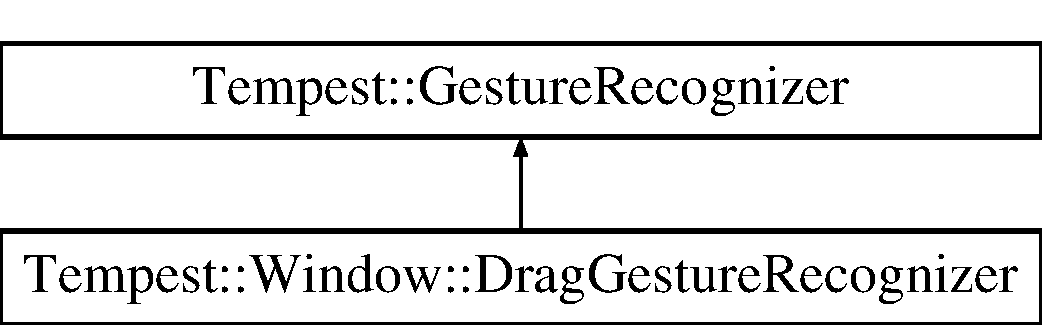
\includegraphics[height=2.000000cm]{class_tempest_1_1_gesture_recognizer}
\end{center}
\end{figure}
\subsection*{Public Member Functions}
\begin{DoxyCompactItemize}
\item 
\hypertarget{class_tempest_1_1_gesture_recognizer_a2bb32488d2e007e488a167f2b6bb1eba}{virtual \hyperlink{class_tempest_1_1_abstract_gesture_event}{Abstract\+Gesture\+Event} $\ast$ {\bfseries event} (const \hyperlink{class_tempest_1_1_event}{Event} \&)}\label{class_tempest_1_1_gesture_recognizer_a2bb32488d2e007e488a167f2b6bb1eba}

\item 
\hypertarget{class_tempest_1_1_gesture_recognizer_a996d9528baa3937a838afbb580b83539}{virtual void {\bfseries delete\+Gesture} (\hyperlink{class_tempest_1_1_abstract_gesture_event}{Abstract\+Gesture\+Event} $\ast$g)}\label{class_tempest_1_1_gesture_recognizer_a996d9528baa3937a838afbb580b83539}

\end{DoxyCompactItemize}


The documentation for this class was generated from the following files\+:\begin{DoxyCompactItemize}
\item 
ui/gesturerecognizer.\+h\item 
ui/gesturerecognizer.\+cpp\end{DoxyCompactItemize}

\hypertarget{class_tempest_1_1_g_l_s_l}{\section{Tempest\+:\+:G\+L\+S\+L Class Reference}
\label{class_tempest_1_1_g_l_s_l}\index{Tempest\+::\+G\+L\+S\+L@{Tempest\+::\+G\+L\+S\+L}}
}
Inheritance diagram for Tempest\+:\+:G\+L\+S\+L\+:\begin{figure}[H]
\begin{center}
\leavevmode
\includegraphics[height=3.000000cm]{class_tempest_1_1_g_l_s_l}
\end{center}
\end{figure}
\subsection*{Classes}
\begin{DoxyCompactItemize}
\item 
struct \hyperlink{struct_g_l_s_l_1_1_data}{Data}
\end{DoxyCompactItemize}
\subsection*{Public Member Functions}
\begin{DoxyCompactItemize}
\item 
\hypertarget{class_tempest_1_1_g_l_s_l_ad1a4daad6c5f0c16610865bcb054a829}{{\bfseries G\+L\+S\+L} (Abstract\+A\+P\+I\+::\+Open\+G\+L2x\+Device $\ast$dev)}\label{class_tempest_1_1_g_l_s_l_ad1a4daad6c5f0c16610865bcb054a829}

\item 
\hypertarget{class_tempest_1_1_g_l_s_l_a139857104558400232263f9fde62c51d}{void {\bfseries begin\+Paint} () const }\label{class_tempest_1_1_g_l_s_l_a139857104558400232263f9fde62c51d}

\item 
\hypertarget{class_tempest_1_1_g_l_s_l_a9fb5903cd532ed11ad856866889ee4c8}{void {\bfseries end\+Paint} () const }\label{class_tempest_1_1_g_l_s_l_a9fb5903cd532ed11ad856866889ee4c8}

\item 
\hypertarget{class_tempest_1_1_g_l_s_l_a57f5dc6afd91e262a14267bc7c1ef8aa}{void {\bfseries enable} () const }\label{class_tempest_1_1_g_l_s_l_a57f5dc6afd91e262a14267bc7c1ef8aa}

\item 
\hypertarget{class_tempest_1_1_g_l_s_l_a2bb4d5cfddaa437df32aa3c506bdd2a0}{void {\bfseries bind} (const \hyperlink{class_tempest_1_1_vertex_shader}{Tempest\+::\+Vertex\+Shader} \&) const }\label{class_tempest_1_1_g_l_s_l_a2bb4d5cfddaa437df32aa3c506bdd2a0}

\item 
\hypertarget{class_tempest_1_1_g_l_s_l_a9d2327740b8d4a508643f684f15e2f47}{void {\bfseries bind} (const \hyperlink{class_tempest_1_1_fragment_shader}{Tempest\+::\+Fragment\+Shader} \&) const }\label{class_tempest_1_1_g_l_s_l_a9d2327740b8d4a508643f684f15e2f47}

\item 
\hypertarget{class_tempest_1_1_g_l_s_l_a048cdadd254cb1092fa4f868f35718fe}{void {\bfseries un\+Bind} (const \hyperlink{class_tempest_1_1_vertex_shader}{Tempest\+::\+Vertex\+Shader} \&) const }\label{class_tempest_1_1_g_l_s_l_a048cdadd254cb1092fa4f868f35718fe}

\item 
\hypertarget{class_tempest_1_1_g_l_s_l_a3a0bbafd9eb83b1aaa79b070da71ceff}{void {\bfseries un\+Bind} (const \hyperlink{class_tempest_1_1_fragment_shader}{Tempest\+::\+Fragment\+Shader} \&) const }\label{class_tempest_1_1_g_l_s_l_a3a0bbafd9eb83b1aaa79b070da71ceff}

\item 
\hypertarget{class_tempest_1_1_g_l_s_l_aa178c5fa5a4db9bd07bc4dcf19f08807}{bool {\bfseries link} (const \hyperlink{class_tempest_1_1_vertex_shader}{Tempest\+::\+Vertex\+Shader} \&vs, const \hyperlink{class_tempest_1_1_fragment_shader}{Tempest\+::\+Fragment\+Shader} \&fs, const Abstract\+A\+P\+I\+::\+Vertex\+Decl $\ast$decl, std\+::string \&log) const }\label{class_tempest_1_1_g_l_s_l_aa178c5fa5a4db9bd07bc4dcf19f08807}

\item 
\hypertarget{class_tempest_1_1_g_l_s_l_a79f93d775f1aead43ac56057b33d2bea}{void {\bfseries set\+Vertex\+Decl} (const Tempest\+::\+Abstract\+A\+P\+I\+::\+Vertex\+Decl $\ast$) const }\label{class_tempest_1_1_g_l_s_l_a79f93d775f1aead43ac56057b33d2bea}

\item 
\hypertarget{class_tempest_1_1_g_l_s_l_afcca5f3279d4f40fc64c1e437a152b5a}{void $\ast$ {\bfseries context} () const }\label{class_tempest_1_1_g_l_s_l_afcca5f3279d4f40fc64c1e437a152b5a}

\item 
\hypertarget{class_tempest_1_1_g_l_s_l_a504b7bb701a4dd27790f9b4310682a0c}{\hyperlink{class_tempest_1_1_vertex_shader}{Vertex\+Shader} $\ast$ {\bfseries create\+Vertex\+Shader\+From\+Source} (const std\+::string \&src, std\+::string \&log) const }\label{class_tempest_1_1_g_l_s_l_a504b7bb701a4dd27790f9b4310682a0c}

\item 
\hypertarget{class_tempest_1_1_g_l_s_l_a6711cb752d0cb897f8ccac0fa3efb4c9}{void {\bfseries delete\+Vertex\+Shader} (\hyperlink{class_tempest_1_1_vertex_shader}{Vertex\+Shader} $\ast$s) const }\label{class_tempest_1_1_g_l_s_l_a6711cb752d0cb897f8ccac0fa3efb4c9}

\item 
\hypertarget{class_tempest_1_1_g_l_s_l_afb8672792ad724e6b76ebef1feae14a8}{\hyperlink{class_tempest_1_1_fragment_shader}{Fragment\+Shader} $\ast$ {\bfseries create\+Fragment\+Shader\+From\+Source} (const std\+::string \&src, std\+::string \&log) const }\label{class_tempest_1_1_g_l_s_l_afb8672792ad724e6b76ebef1feae14a8}

\item 
\hypertarget{class_tempest_1_1_g_l_s_l_af40b92f09afee1937c0c6651137b4a01}{void {\bfseries delete\+Fragment\+Shader} (\hyperlink{class_tempest_1_1_fragment_shader}{Fragment\+Shader} $\ast$s) const }\label{class_tempest_1_1_g_l_s_l_af40b92f09afee1937c0c6651137b4a01}

\item 
\hypertarget{class_tempest_1_1_g_l_s_l_ae564a02582020c313d119050fbf5ed89}{std\+::string {\bfseries surface\+Shader} (Shader\+Type t, const \hyperlink{struct_tempest_1_1_abstract_shading_lang_1_1_ui_shader_opt}{Ui\+Shader\+Opt} \&, bool \&has\+Halfpix\+Offset) const }\label{class_tempest_1_1_g_l_s_l_ae564a02582020c313d119050fbf5ed89}

\end{DoxyCompactItemize}
\subsection*{Additional Inherited Members}


The documentation for this class was generated from the following files\+:\begin{DoxyCompactItemize}
\item 
ogl/glsl.\+h\item 
ogl/glsl.\+cpp\end{DoxyCompactItemize}

\hypertarget{class_tempest_1_1_graphic_object}{\section{Tempest\+:\+:Graphic\+Object$<$ Material, User\+State $>$ Class Template Reference}
\label{class_tempest_1_1_graphic_object}\index{Tempest\+::\+Graphic\+Object$<$ Material, User\+State $>$@{Tempest\+::\+Graphic\+Object$<$ Material, User\+State $>$}}
}
Inheritance diagram for Tempest\+:\+:Graphic\+Object$<$ Material, User\+State $>$\+:\begin{figure}[H]
\begin{center}
\leavevmode
\includegraphics[height=3.000000cm]{class_tempest_1_1_graphic_object}
\end{center}
\end{figure}
\subsection*{Public Types}
\begin{DoxyCompactItemize}
\item 
\hypertarget{class_tempest_1_1_graphic_object_a27920036e893aa5e9a7f85ad7316f562}{typedef \hyperlink{class_tempest_1_1_abstract_scene}{Abstract\+Scene}\\*
$<$ \hyperlink{class_tempest_1_1_abstract_graphic_object}{Abstract\+Graphic\+Object}\\*
$<$ Material, User\+State $>$ $>$ {\bfseries Scene}}\label{class_tempest_1_1_graphic_object_a27920036e893aa5e9a7f85ad7316f562}

\end{DoxyCompactItemize}
\subsection*{Public Member Functions}
\begin{DoxyCompactItemize}
\item 
\hypertarget{class_tempest_1_1_graphic_object_a8bd08f5548374eb91b33812747ff6284}{{\bfseries Graphic\+Object} (\hyperlink{class_tempest_1_1_abstract_scene}{Scene} \&s)}\label{class_tempest_1_1_graphic_object_a8bd08f5548374eb91b33812747ff6284}

\item 
\hypertarget{class_tempest_1_1_graphic_object_a7ac61ff9474025d9d18d76d9c3deff32}{{\bfseries Graphic\+Object} (const \hyperlink{class_tempest_1_1_graphic_object}{Graphic\+Object} \&obj)}\label{class_tempest_1_1_graphic_object_a7ac61ff9474025d9d18d76d9c3deff32}

\item 
\hypertarget{class_tempest_1_1_graphic_object_ab7779a7b30d0b32051dc48149909d708}{\hyperlink{class_tempest_1_1_graphic_object}{Graphic\+Object} \& {\bfseries operator=} (const \hyperlink{class_tempest_1_1_graphic_object}{Graphic\+Object} \&g)}\label{class_tempest_1_1_graphic_object_ab7779a7b30d0b32051dc48149909d708}

\item 
\hypertarget{class_tempest_1_1_graphic_object_a685481826e5ce876ff28c67a9b2a4b09}{{\footnotesize template$<$class V $>$ }\\void {\bfseries set\+Model} (const \hyperlink{class_tempest_1_1_model}{Model}$<$ V $>$ \&md)}\label{class_tempest_1_1_graphic_object_a685481826e5ce876ff28c67a9b2a4b09}

\item 
\hypertarget{class_tempest_1_1_graphic_object_a5a9915e2a2c8fca687e87928bc9219e9}{const \hyperlink{struct_tempest_1_1_model_bounds}{Model\+Bounds} \& {\bfseries bounds} () const }\label{class_tempest_1_1_graphic_object_a5a9915e2a2c8fca687e87928bc9219e9}

\item 
\hypertarget{class_tempest_1_1_graphic_object_a395e630eee08bffd4076be471b23a421}{const \hyperlink{class_tempest_1_1_matrix4x4}{Matrix4x4} \& {\bfseries transform} () const }\label{class_tempest_1_1_graphic_object_a395e630eee08bffd4076be471b23a421}

\item 
\hypertarget{class_tempest_1_1_graphic_object_a05248a0f457a84c3265dcbc1f775891e}{virtual void {\bfseries set\+Position} (double x, double y, double z)}\label{class_tempest_1_1_graphic_object_a05248a0f457a84c3265dcbc1f775891e}

\item 
\hypertarget{class_tempest_1_1_graphic_object_afe9a7ad8306b8bf603a33c75f4878bed}{virtual void {\bfseries set\+Size} (double x, double y, double z)}\label{class_tempest_1_1_graphic_object_afe9a7ad8306b8bf603a33c75f4878bed}

\item 
\hypertarget{class_tempest_1_1_graphic_object_ab1076aa36d615730bd82a5ba23078fe9}{virtual void {\bfseries set\+Size} (double s)}\label{class_tempest_1_1_graphic_object_ab1076aa36d615730bd82a5ba23078fe9}

\item 
\hypertarget{class_tempest_1_1_graphic_object_a919e48d3524948ed837fc2b0e6ef9687}{virtual void {\bfseries set\+Rotation} (double x, double z)}\label{class_tempest_1_1_graphic_object_a919e48d3524948ed837fc2b0e6ef9687}

\item 
\hypertarget{class_tempest_1_1_graphic_object_aa48dee9b537a5d002880356a050a03a8}{virtual void {\bfseries set\+Rotation} (double x, double y, double z)}\label{class_tempest_1_1_graphic_object_aa48dee9b537a5d002880356a050a03a8}

\item 
\hypertarget{class_tempest_1_1_graphic_object_a530c4c11a9940b4fbefa384d6b9b658b}{virtual float {\bfseries x} () const }\label{class_tempest_1_1_graphic_object_a530c4c11a9940b4fbefa384d6b9b658b}

\item 
\hypertarget{class_tempest_1_1_graphic_object_a2abbef896c0c7be53e9094b432f2e7c3}{virtual float {\bfseries y} () const }\label{class_tempest_1_1_graphic_object_a2abbef896c0c7be53e9094b432f2e7c3}

\item 
\hypertarget{class_tempest_1_1_graphic_object_a16d3244b05a076706dcd09ace6ecb25c}{virtual float {\bfseries z} () const }\label{class_tempest_1_1_graphic_object_a16d3244b05a076706dcd09ace6ecb25c}

\item 
\hypertarget{class_tempest_1_1_graphic_object_a18120dfb414b7ebd314f80acd6b808a7}{virtual float {\bfseries size\+X} () const }\label{class_tempest_1_1_graphic_object_a18120dfb414b7ebd314f80acd6b808a7}

\item 
\hypertarget{class_tempest_1_1_graphic_object_a0d58c741edbee85bfbaa9b2ebd4b52dd}{virtual float {\bfseries size\+Y} () const }\label{class_tempest_1_1_graphic_object_a0d58c741edbee85bfbaa9b2ebd4b52dd}

\item 
\hypertarget{class_tempest_1_1_graphic_object_acb892c8478a35709d3960d0799234690}{virtual float {\bfseries size\+Z} () const }\label{class_tempest_1_1_graphic_object_acb892c8478a35709d3960d0799234690}

\item 
\hypertarget{class_tempest_1_1_graphic_object_a8693934f5b669c05eeba009f044f122b}{virtual float {\bfseries angle\+X} () const }\label{class_tempest_1_1_graphic_object_a8693934f5b669c05eeba009f044f122b}

\item 
\hypertarget{class_tempest_1_1_graphic_object_a2bcccbc084fc76365a700e8d195e3748}{virtual float {\bfseries angle\+Y} () const }\label{class_tempest_1_1_graphic_object_a2bcccbc084fc76365a700e8d195e3748}

\item 
\hypertarget{class_tempest_1_1_graphic_object_a183d2ac469344f579743ac4a5ef2806f}{virtual float {\bfseries angle\+Z} () const }\label{class_tempest_1_1_graphic_object_a183d2ac469344f579743ac4a5ef2806f}

\item 
\hypertarget{class_tempest_1_1_graphic_object_ab8f72a0102f10a0e862406e5b0bca99e}{virtual float {\bfseries radius} () const }\label{class_tempest_1_1_graphic_object_ab8f72a0102f10a0e862406e5b0bca99e}

\item 
\hypertarget{class_tempest_1_1_graphic_object_a166c681f17eb40155f596d1c92cb27aa}{virtual void {\bfseries render} (\hyperlink{class_tempest_1_1_device}{Device} \&dev, \hyperlink{class_tempest_1_1_program_object}{Program\+Object} \&p) const }\label{class_tempest_1_1_graphic_object_a166c681f17eb40155f596d1c92cb27aa}

\item 
\hypertarget{class_tempest_1_1_graphic_object_aa1daf9c938c6520ca42bcc1332464909}{virtual void {\bfseries render} (\hyperlink{class_tempest_1_1_device}{Device} \&dev, \hyperlink{class_tempest_1_1_vertex_shader}{Vertex\+Shader} \&vs, \hyperlink{class_tempest_1_1_fragment_shader}{Fragment\+Shader} \&fs) const }\label{class_tempest_1_1_graphic_object_aa1daf9c938c6520ca42bcc1332464909}

\end{DoxyCompactItemize}
\subsection*{Protected Member Functions}
\begin{DoxyCompactItemize}
\item 
\hypertarget{class_tempest_1_1_graphic_object_aad5a56638462c930c98ff7df72bce82f}{virtual \hyperlink{class_tempest_1_1_matrix4x4}{Tempest\+::\+Matrix4x4} {\bfseries compute\+Mat} () const }\label{class_tempest_1_1_graphic_object_aad5a56638462c930c98ff7df72bce82f}

\item 
\hypertarget{class_tempest_1_1_graphic_object_ae686b02ae09d62eb9d50585355ecc748}{void {\bfseries request\+Matrix\+Update} ()}\label{class_tempest_1_1_graphic_object_ae686b02ae09d62eb9d50585355ecc748}

\end{DoxyCompactItemize}
\subsection*{Additional Inherited Members}


The documentation for this class was generated from the following file\+:\begin{DoxyCompactItemize}
\item 
scene/graphicobject.\+h\end{DoxyCompactItemize}

\hypertarget{class_tempest_1_1_graphics_subsystem}{\section{Tempest\+:\+:Graphics\+Subsystem Class Reference}
\label{class_tempest_1_1_graphics_subsystem}\index{Tempest\+::\+Graphics\+Subsystem@{Tempest\+::\+Graphics\+Subsystem}}
}
Inheritance diagram for Tempest\+:\+:Graphics\+Subsystem\+:\begin{figure}[H]
\begin{center}
\leavevmode
\includegraphics[height=1.740933cm]{class_tempest_1_1_graphics_subsystem}
\end{center}
\end{figure}
\subsection*{Classes}
\begin{DoxyCompactItemize}
\item 
struct \hyperlink{struct_tempest_1_1_graphics_subsystem_1_1_delete_event}{Delete\+Event}
\item 
struct \hyperlink{struct_tempest_1_1_graphics_subsystem_1_1_event}{Event}
\end{DoxyCompactItemize}
\subsection*{Public Types}
\begin{DoxyCompactItemize}
\item 
\hypertarget{class_tempest_1_1_graphics_subsystem_a92ffbf28fb07334ab59c23051eb089c3}{enum {\bfseries Shader\+Type} \{ {\bfseries Vertex}, 
{\bfseries Fragment}
 \}}\label{class_tempest_1_1_graphics_subsystem_a92ffbf28fb07334ab59c23051eb089c3}

\end{DoxyCompactItemize}
\subsection*{Public Member Functions}
\begin{DoxyCompactItemize}
\item 
\hypertarget{class_tempest_1_1_graphics_subsystem_a8c7b7a5fee3e9b20f9946c6fc2152cc0}{virtual void {\bfseries event} (const \hyperlink{struct_tempest_1_1_graphics_subsystem_1_1_event}{Event} \&e)}\label{class_tempest_1_1_graphics_subsystem_a8c7b7a5fee3e9b20f9946c6fc2152cc0}

\item 
\hypertarget{class_tempest_1_1_graphics_subsystem_a927c91646e25c44e94ffdcdfe9dffdc2}{virtual void {\bfseries event} (const \hyperlink{struct_tempest_1_1_graphics_subsystem_1_1_delete_event}{Delete\+Event} \&e)}\label{class_tempest_1_1_graphics_subsystem_a927c91646e25c44e94ffdcdfe9dffdc2}

\end{DoxyCompactItemize}


The documentation for this class was generated from the following files\+:\begin{DoxyCompactItemize}
\item 
core/graphicssubsystem.\+h\item 
core/graphicssubsystem.\+cpp\end{DoxyCompactItemize}

\hypertarget{class_tempest_1_1_half}{\section{Tempest\+:\+:Half Class Reference}
\label{class_tempest_1_1_half}\index{Tempest\+::\+Half@{Tempest\+::\+Half}}
}
\subsection*{Public Member Functions}
\begin{DoxyCompactItemize}
\item 
\hypertarget{class_tempest_1_1_half_a869653150ec9cf24a176dbb71a996ddc}{\hyperlink{class_tempest_1_1_half}{Half} \& {\bfseries operator=} (float fin)}\label{class_tempest_1_1_half_a869653150ec9cf24a176dbb71a996ddc}

\item 
\hypertarget{class_tempest_1_1_half_a523358e7b62072f0625cab16a91b511a}{{\bfseries operator float} () const }\label{class_tempest_1_1_half_a523358e7b62072f0625cab16a91b511a}

\end{DoxyCompactItemize}
\subsection*{Public Attributes}
\begin{DoxyCompactItemize}
\item 
\hypertarget{class_tempest_1_1_half_a050d462427f78f6f0b204922f44e9bb6}{uint16\+\_\+t {\bfseries v}}\label{class_tempest_1_1_half_a050d462427f78f6f0b204922f44e9bb6}

\end{DoxyCompactItemize}
\subsection*{Static Public Attributes}
\begin{DoxyCompactItemize}
\item 
\hypertarget{class_tempest_1_1_half_a0dd56ae8eedd8a0f63579e06c133c9b5}{static const unsigned int {\bfseries M\+I\+N\+\_\+\+B\+I\+A\+S\+E\+D\+\_\+\+E\+X\+P\+\_\+\+A\+S\+\_\+\+S\+I\+N\+G\+L\+E\+\_\+\+F\+P\+\_\+\+E\+X\+P} = 0x38000000}\label{class_tempest_1_1_half_a0dd56ae8eedd8a0f63579e06c133c9b5}

\item 
\hypertarget{class_tempest_1_1_half_a0d9498ac5d299c34fdf0ea97016f4160}{static const unsigned int {\bfseries M\+A\+X\+\_\+\+B\+I\+A\+S\+E\+D\+\_\+\+E\+X\+P\+\_\+\+A\+S\+\_\+\+S\+I\+N\+G\+L\+E\+\_\+\+F\+P\+\_\+\+E\+X\+P} = 0x47800000}\label{class_tempest_1_1_half_a0d9498ac5d299c34fdf0ea97016f4160}

\item 
\hypertarget{class_tempest_1_1_half_a169211a32cc92672c655a9a120e5d2a0}{static const unsigned int {\bfseries F\+L\+O\+A\+T\+\_\+\+M\+A\+X\+\_\+\+B\+I\+A\+S\+E\+D\+\_\+\+E\+X\+P} = (0x\+F\+F $<$$<$ 23)}\label{class_tempest_1_1_half_a169211a32cc92672c655a9a120e5d2a0}

\item 
\hypertarget{class_tempest_1_1_half_a4b318c4fd28a8d725c62e7c5427a71ae}{static const unsigned int {\bfseries H\+A\+L\+F\+\_\+\+F\+L\+O\+A\+T\+\_\+\+M\+A\+X\+\_\+\+B\+I\+A\+S\+E\+D\+\_\+\+E\+X\+P} = (0x1\+F $<$$<$ 10)}\label{class_tempest_1_1_half_a4b318c4fd28a8d725c62e7c5427a71ae}

\end{DoxyCompactItemize}


The documentation for this class was generated from the following file\+:\begin{DoxyCompactItemize}
\item 
core/wrappers/half.\+h\end{DoxyCompactItemize}

\hypertarget{class_tempest_1_1_h_l_s_l}{\section{Tempest\+:\+:H\+L\+S\+L Class Reference}
\label{class_tempest_1_1_h_l_s_l}\index{Tempest\+::\+H\+L\+S\+L@{Tempest\+::\+H\+L\+S\+L}}
}
Inheritance diagram for Tempest\+:\+:H\+L\+S\+L\+:\begin{figure}[H]
\begin{center}
\leavevmode
\includegraphics[height=3.000000cm]{class_tempest_1_1_h_l_s_l}
\end{center}
\end{figure}
\subsection*{Classes}
\begin{DoxyCompactItemize}
\item 
struct \hyperlink{struct_h_l_s_l_1_1_data}{Data}
\end{DoxyCompactItemize}
\subsection*{Public Member Functions}
\begin{DoxyCompactItemize}
\item 
\hypertarget{class_tempest_1_1_h_l_s_l_a8bab5c8f23d7f9a325aa8c6f5be15b0a}{{\bfseries H\+L\+S\+L} (Abstract\+A\+P\+I\+::\+Direct\+X9\+Device $\ast$dev)}\label{class_tempest_1_1_h_l_s_l_a8bab5c8f23d7f9a325aa8c6f5be15b0a}

\item 
\hypertarget{class_tempest_1_1_h_l_s_l_a573baa77cb78144c122ebd9d61a178fd}{void {\bfseries enable} () const }\label{class_tempest_1_1_h_l_s_l_a573baa77cb78144c122ebd9d61a178fd}

\item 
\hypertarget{class_tempest_1_1_h_l_s_l_a09d93e28311a5653b5ccd2b268dd37f3}{void {\bfseries bind} (const \hyperlink{class_tempest_1_1_vertex_shader}{Tempest\+::\+Vertex\+Shader} \&) const }\label{class_tempest_1_1_h_l_s_l_a09d93e28311a5653b5ccd2b268dd37f3}

\item 
\hypertarget{class_tempest_1_1_h_l_s_l_a9dfd518a6457f9a320571c9f44bf258d}{void {\bfseries bind} (const \hyperlink{class_tempest_1_1_fragment_shader}{Tempest\+::\+Fragment\+Shader} \&) const }\label{class_tempest_1_1_h_l_s_l_a9dfd518a6457f9a320571c9f44bf258d}

\item 
\hypertarget{class_tempest_1_1_h_l_s_l_a2a139bbd076b59e199e3c5f20732f7bd}{void {\bfseries un\+Bind} (const \hyperlink{class_tempest_1_1_vertex_shader}{Tempest\+::\+Vertex\+Shader} \&) const }\label{class_tempest_1_1_h_l_s_l_a2a139bbd076b59e199e3c5f20732f7bd}

\item 
\hypertarget{class_tempest_1_1_h_l_s_l_a4434e7de0fe954da7619392cf9d49ec6}{void {\bfseries un\+Bind} (const \hyperlink{class_tempest_1_1_fragment_shader}{Tempest\+::\+Fragment\+Shader} \&) const }\label{class_tempest_1_1_h_l_s_l_a4434e7de0fe954da7619392cf9d49ec6}

\item 
\hypertarget{class_tempest_1_1_h_l_s_l_a7447df6d35d750309b548218e7bf7123}{void $\ast$ {\bfseries context} () const }\label{class_tempest_1_1_h_l_s_l_a7447df6d35d750309b548218e7bf7123}

\item 
\hypertarget{class_tempest_1_1_h_l_s_l_af66fd7d08dfe8c4006db010ef52dff9c}{\hyperlink{class_tempest_1_1_vertex_shader}{Vertex\+Shader} $\ast$ {\bfseries create\+Vertex\+Shader\+From\+Source} (const std\+::string \&src, std\+::string \&output\+Log) const }\label{class_tempest_1_1_h_l_s_l_af66fd7d08dfe8c4006db010ef52dff9c}

\item 
\hypertarget{class_tempest_1_1_h_l_s_l_a728ac5e8a4efd116cfe8d55679f3a0b2}{void {\bfseries delete\+Vertex\+Shader} (\hyperlink{class_tempest_1_1_vertex_shader}{Vertex\+Shader} $\ast$s) const }\label{class_tempest_1_1_h_l_s_l_a728ac5e8a4efd116cfe8d55679f3a0b2}

\item 
\hypertarget{class_tempest_1_1_h_l_s_l_a3ea4e98838da54ed7e79fabe46a3a389}{\hyperlink{class_tempest_1_1_fragment_shader}{Fragment\+Shader} $\ast$ {\bfseries create\+Fragment\+Shader\+From\+Source} (const std\+::string \&src, std\+::string \&output\+Log) const }\label{class_tempest_1_1_h_l_s_l_a3ea4e98838da54ed7e79fabe46a3a389}

\item 
\hypertarget{class_tempest_1_1_h_l_s_l_a66b682bc7c749ab1b016ab79e6d7c901}{void {\bfseries delete\+Fragment\+Shader} (\hyperlink{class_tempest_1_1_fragment_shader}{Fragment\+Shader} $\ast$s) const }\label{class_tempest_1_1_h_l_s_l_a66b682bc7c749ab1b016ab79e6d7c901}

\item 
\hypertarget{class_tempest_1_1_h_l_s_l_a7b8fb84c7e3c992ece821dd1278c39a8}{std\+::string {\bfseries surface\+Shader} (Shader\+Type t, const \hyperlink{struct_tempest_1_1_abstract_shading_lang_1_1_ui_shader_opt}{Ui\+Shader\+Opt} \&, bool \&has\+Halfpix\+Offset) const }\label{class_tempest_1_1_h_l_s_l_a7b8fb84c7e3c992ece821dd1278c39a8}

\end{DoxyCompactItemize}
\subsection*{Additional Inherited Members}


The documentation for this class was generated from the following files\+:\begin{DoxyCompactItemize}
\item 
dx/hlsl.\+h\item 
dx/hlsl.\+cpp\end{DoxyCompactItemize}

\hypertarget{struct_direct_x9_1_1_i_b_o}{\section{Tempest\+:\+:Direct\+X9\+:\+:I\+B\+O Struct Reference}
\label{struct_direct_x9_1_1_i_b_o}\index{Tempest\+::\+Direct\+X9\+::\+I\+B\+O@{Tempest\+::\+Direct\+X9\+::\+I\+B\+O}}
}
\subsection*{Classes}
\begin{DoxyCompactItemize}
\item 
struct \hyperlink{struct_direct_x9_1_1_i_b_o_1_1_min}{Min}
\end{DoxyCompactItemize}
\subsection*{Public Attributes}
\begin{DoxyCompactItemize}
\item 
\hypertarget{struct_direct_x9_1_1_i_b_o_a0c6ac00a8cdc16abb662de9868deb33e}{L\+P\+D\+I\+R\+E\+C\+T3\+D\+I\+N\+D\+E\+X\+B\+U\+F\+F\+E\+R9 {\bfseries index}}\label{struct_direct_x9_1_1_i_b_o_a0c6ac00a8cdc16abb662de9868deb33e}

\item 
\hypertarget{struct_direct_x9_1_1_i_b_o_a2993a38160e5efe253d8156577599b7c}{std\+::vector$<$ uint16\+\_\+t $>$ {\bfseries pbuf}}\label{struct_direct_x9_1_1_i_b_o_a2993a38160e5efe253d8156577599b7c}

\item 
\hypertarget{struct_direct_x9_1_1_i_b_o_aeaeb233b5290ea22cef8bf7bac259443}{std\+::vector$<$ \hyperlink{struct_direct_x9_1_1_i_b_o_1_1_min}{Min} $>$ {\bfseries min}}\label{struct_direct_x9_1_1_i_b_o_aeaeb233b5290ea22cef8bf7bac259443}

\end{DoxyCompactItemize}


The documentation for this struct was generated from the following file\+:\begin{DoxyCompactItemize}
\item 
dx/directx9.\+cpp\end{DoxyCompactItemize}

\hypertarget{class_tempest_1_1_i_device}{\section{Tempest\+:\+:I\+Device Class Reference}
\label{class_tempest_1_1_i_device}\index{Tempest\+::\+I\+Device@{Tempest\+::\+I\+Device}}
}
Inheritance diagram for Tempest\+:\+:I\+Device\+:\begin{figure}[H]
\begin{center}
\leavevmode
\includegraphics[height=1.953488cm]{class_tempest_1_1_i_device}
\end{center}
\end{figure}
\subsection*{Public Member Functions}
\begin{DoxyCompactItemize}
\item 
\hypertarget{class_tempest_1_1_i_device_a0d8757120f5723b40457661052de8f96}{virtual size\+\_\+t {\bfseries read\+Data} (char $\ast$dest, size\+\_\+t count)=0}\label{class_tempest_1_1_i_device_a0d8757120f5723b40457661052de8f96}

\item 
\hypertarget{class_tempest_1_1_i_device_ab5848e89bae0b736447a42d3619836b9}{virtual void {\bfseries skip} (size\+\_\+t count)=0}\label{class_tempest_1_1_i_device_ab5848e89bae0b736447a42d3619836b9}

\item 
\hypertarget{class_tempest_1_1_i_device_a86b8d56eb4bb292d3dfa8e900d0d7bb6}{virtual char {\bfseries peek} () const }\label{class_tempest_1_1_i_device_a86b8d56eb4bb292d3dfa8e900d0d7bb6}

\item 
\hypertarget{class_tempest_1_1_i_device_a8ff3eaf2a35f42cdb61af5da685b4b71}{virtual size\+\_\+t {\bfseries peek} (size\+\_\+t skip, char $\ast$dest, size\+\_\+t max\+Size) const =0}\label{class_tempest_1_1_i_device_a8ff3eaf2a35f42cdb61af5da685b4b71}

\end{DoxyCompactItemize}


The documentation for this class was generated from the following files\+:\begin{DoxyCompactItemize}
\item 
io/iodevice.\+h\item 
io/iodevice.\+cpp\end{DoxyCompactItemize}

\hypertarget{class_tempest_1_1_image}{\section{Tempest\+:\+:Image$<$ In\+Texture $>$ Class Template Reference}
\label{class_tempest_1_1_image}\index{Tempest\+::\+Image$<$ In\+Texture $>$@{Tempest\+::\+Image$<$ In\+Texture $>$}}
}
Inheritance diagram for Tempest\+:\+:Image$<$ In\+Texture $>$\+:\begin{figure}[H]
\begin{center}
\leavevmode
\includegraphics[height=2.000000cm]{class_tempest_1_1_image}
\end{center}
\end{figure}
\subsection*{Public Types}
\begin{DoxyCompactItemize}
\item 
\hypertarget{class_tempest_1_1_image_afdc4124969ddb46505027e94df5ce192}{typedef In\+Texture {\bfseries Texture}}\label{class_tempest_1_1_image_afdc4124969ddb46505027e94df5ce192}

\end{DoxyCompactItemize}
\subsection*{Public Member Functions}
\begin{DoxyCompactItemize}
\item 
\hypertarget{class_tempest_1_1_image_af851d98fa6c7fb1e66487831aa3ac396}{void {\bfseries mouse\+Down\+Event} (\hyperlink{class_tempest_1_1_mouse_event}{Mouse\+Event} \&e)}\label{class_tempest_1_1_image_af851d98fa6c7fb1e66487831aa3ac396}

\item 
\hypertarget{class_tempest_1_1_image_af26d8f04022a0b1cd06089eac8ecdbf1}{void {\bfseries mouse\+Up\+Event} (\hyperlink{class_tempest_1_1_mouse_event}{Mouse\+Event} \&e)}\label{class_tempest_1_1_image_af26d8f04022a0b1cd06089eac8ecdbf1}

\item 
\hypertarget{class_tempest_1_1_image_aac34676b7db6a0184013a0e2dcc87888}{void {\bfseries mouse\+Move\+Event} (\hyperlink{class_tempest_1_1_mouse_event}{Mouse\+Event} \&e)}\label{class_tempest_1_1_image_aac34676b7db6a0184013a0e2dcc87888}

\end{DoxyCompactItemize}
\subsection*{Public Attributes}
\begin{DoxyCompactItemize}
\item 
\hypertarget{class_tempest_1_1_image_a96077ffe91e97fd914a9f993d3c901bb}{Texture {\bfseries texture}}\label{class_tempest_1_1_image_a96077ffe91e97fd914a9f993d3c901bb}

\end{DoxyCompactItemize}
\subsection*{Protected Member Functions}
\begin{DoxyCompactItemize}
\item 
\hypertarget{class_tempest_1_1_image_ad9bd93e8a170f239299ffb008fe477b6}{void {\bfseries paint\+Event} (\hyperlink{class_tempest_1_1_paint_event}{Paint\+Event} \&pe)}\label{class_tempest_1_1_image_ad9bd93e8a170f239299ffb008fe477b6}

\end{DoxyCompactItemize}


The documentation for this class was generated from the following file\+:\begin{DoxyCompactItemize}
\item 
ui/image.\+h\end{DoxyCompactItemize}

\hypertarget{class_tempest_1_1_image_codec}{\section{Tempest\+:\+:Image\+Codec Class Reference}
\label{class_tempest_1_1_image_codec}\index{Tempest\+::\+Image\+Codec@{Tempest\+::\+Image\+Codec}}
}
Inheritance diagram for Tempest\+:\+:Image\+Codec\+:\begin{figure}[H]
\begin{center}
\leavevmode
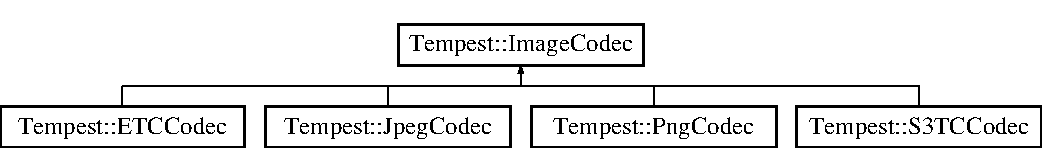
\includegraphics[height=1.971831cm]{class_tempest_1_1_image_codec}
\end{center}
\end{figure}
\subsection*{Public Types}
\begin{DoxyCompactItemize}
\item 
\hypertarget{class_tempest_1_1_image_codec_a1fce4efcec49dc1c9399eb417bcf1148}{typedef \hyperlink{struct_tempest_1_1_pixmap_1_1_img_info}{Pixmap\+::\+Img\+Info} {\bfseries Img\+Info}}\label{class_tempest_1_1_image_codec_a1fce4efcec49dc1c9399eb417bcf1148}

\end{DoxyCompactItemize}
\subsection*{Public Member Functions}
\begin{DoxyCompactItemize}
\item 
\hypertarget{class_tempest_1_1_image_codec_a261f66638aeced8e3f620b6f365cebbc}{virtual bool {\bfseries can\+Save} (const \hyperlink{struct_tempest_1_1_pixmap_1_1_img_info}{Img\+Info} \&) const }\label{class_tempest_1_1_image_codec_a261f66638aeced8e3f620b6f365cebbc}

\item 
\hypertarget{class_tempest_1_1_image_codec_a39bb950f18cec34627e0eee4f11fa9a2}{virtual bool {\bfseries can\+Convert\+To} (const \hyperlink{struct_tempest_1_1_pixmap_1_1_img_info}{Img\+Info} \&, Pixmap\+::\+Format fout) const }\label{class_tempest_1_1_image_codec_a39bb950f18cec34627e0eee4f11fa9a2}

\item 
\hypertarget{class_tempest_1_1_image_codec_a15f2dffe195ef4a0d91a778842f404b4}{virtual void {\bfseries to\+R\+G\+B} (\hyperlink{struct_tempest_1_1_pixmap_1_1_img_info}{Img\+Info} \&info, std\+::vector$<$ unsigned char $>$ \&inout, bool alpha)}\label{class_tempest_1_1_image_codec_a15f2dffe195ef4a0d91a778842f404b4}

\item 
\hypertarget{class_tempest_1_1_image_codec_a39693611734757d1631b9164227bbac0}{virtual void {\bfseries from\+R\+G\+B} (\hyperlink{struct_tempest_1_1_pixmap_1_1_img_info}{Img\+Info} \&info, std\+::vector$<$ unsigned char $>$ \&inout)}\label{class_tempest_1_1_image_codec_a39693611734757d1631b9164227bbac0}

\item 
\hypertarget{class_tempest_1_1_image_codec_ab6e62bd073a749f77ecf568a21d2b3f1}{virtual bool {\bfseries load} (\hyperlink{class_tempest_1_1_i_device}{I\+Device} \&img\+Bytes, \hyperlink{struct_tempest_1_1_pixmap_1_1_img_info}{Img\+Info} \&info, std\+::vector$<$ unsigned char $>$ \&out)}\label{class_tempest_1_1_image_codec_ab6e62bd073a749f77ecf568a21d2b3f1}

\item 
\hypertarget{class_tempest_1_1_image_codec_a1497e6829f9f1fddaa1267d487cde493}{virtual bool {\bfseries save} (\hyperlink{class_tempest_1_1_o_device}{O\+Device} \&file, const \hyperlink{struct_tempest_1_1_pixmap_1_1_img_info}{Img\+Info} \&info, const std\+::vector$<$ unsigned char $>$ \&img)}\label{class_tempest_1_1_image_codec_a1497e6829f9f1fddaa1267d487cde493}

\end{DoxyCompactItemize}
\subsection*{Static Public Member Functions}
\begin{DoxyCompactItemize}
\item 
\hypertarget{class_tempest_1_1_image_codec_a057e58ed4f0d2b03593a2d319884a7ee}{static void {\bfseries install\+Std\+Codecs} (\hyperlink{class_tempest_1_1_system_a_p_i}{System\+A\+P\+I} \&s)}\label{class_tempest_1_1_image_codec_a057e58ed4f0d2b03593a2d319884a7ee}

\item 
\hypertarget{class_tempest_1_1_image_codec_ac3284f39ff91673c631118cdad7a9d2d}{static void {\bfseries add\+Alpha} (\hyperlink{struct_tempest_1_1_pixmap_1_1_img_info}{Img\+Info} \&info, std\+::vector$<$ unsigned char $>$ \&rgb)}\label{class_tempest_1_1_image_codec_ac3284f39ff91673c631118cdad7a9d2d}

\item 
\hypertarget{class_tempest_1_1_image_codec_abdcefe6087cb2c924641d9ee49a39cf5}{static void {\bfseries remove\+Alpha} (\hyperlink{struct_tempest_1_1_pixmap_1_1_img_info}{Img\+Info} \&info, std\+::vector$<$ unsigned char $>$ \&rgba)}\label{class_tempest_1_1_image_codec_abdcefe6087cb2c924641d9ee49a39cf5}

\item 
\hypertarget{class_tempest_1_1_image_codec_a7f6fe78948c973521a5344acc9b1cc0e}{static void {\bfseries resize} (\hyperlink{struct_tempest_1_1_pixmap_1_1_img_info}{Img\+Info} \&info, std\+::vector$<$ unsigned char $>$ \&rgb, int nw, int nh)}\label{class_tempest_1_1_image_codec_a7f6fe78948c973521a5344acc9b1cc0e}

\item 
\hypertarget{class_tempest_1_1_image_codec_aa655d054444380a8af3e909b47213332}{static void {\bfseries downsample} (\hyperlink{struct_tempest_1_1_pixmap_1_1_img_info}{Img\+Info} \&info, std\+::vector$<$ unsigned char $>$ \&rgb)}\label{class_tempest_1_1_image_codec_aa655d054444380a8af3e909b47213332}

\end{DoxyCompactItemize}


The documentation for this class was generated from the following files\+:\begin{DoxyCompactItemize}
\item 
core/imagecodec.\+h\item 
core/imagecodec.\+cpp\end{DoxyCompactItemize}

\hypertarget{struct_tempest_1_1_pixmap_1_1_img_info}{\section{Tempest\+:\+:Pixmap\+:\+:Img\+Info Struct Reference}
\label{struct_tempest_1_1_pixmap_1_1_img_info}\index{Tempest\+::\+Pixmap\+::\+Img\+Info@{Tempest\+::\+Pixmap\+::\+Img\+Info}}
}
\subsection*{Public Attributes}
\begin{DoxyCompactItemize}
\item 
\hypertarget{struct_tempest_1_1_pixmap_1_1_img_info_a4b773c6cfce7063bd6dec9689e8783ff}{int {\bfseries w}}\label{struct_tempest_1_1_pixmap_1_1_img_info_a4b773c6cfce7063bd6dec9689e8783ff}

\item 
\hypertarget{struct_tempest_1_1_pixmap_1_1_img_info_ae2d796b27cfcc35d10e500894464bde5}{int {\bfseries h}}\label{struct_tempest_1_1_pixmap_1_1_img_info_ae2d796b27cfcc35d10e500894464bde5}

\item 
\hypertarget{struct_tempest_1_1_pixmap_1_1_img_info_a39a853c8bb323aebf4c007aaab4f29d4}{int {\bfseries bpp}}\label{struct_tempest_1_1_pixmap_1_1_img_info_a39a853c8bb323aebf4c007aaab4f29d4}

\item 
\hypertarget{struct_tempest_1_1_pixmap_1_1_img_info_a65d38b8faed2ace2f29bdc6d0a9e0192}{int {\bfseries mip\+Levels}}\label{struct_tempest_1_1_pixmap_1_1_img_info_a65d38b8faed2ace2f29bdc6d0a9e0192}

\item 
\hypertarget{struct_tempest_1_1_pixmap_1_1_img_info_a3ac71c6e52c4c869778e347f01c83437}{bool {\bfseries alpha}}\label{struct_tempest_1_1_pixmap_1_1_img_info_a3ac71c6e52c4c869778e347f01c83437}

\item 
\hypertarget{struct_tempest_1_1_pixmap_1_1_img_info_aae2b042545b3eeb3ea26c754bd3746d4}{Pixmap\+::\+Format {\bfseries format}}\label{struct_tempest_1_1_pixmap_1_1_img_info_aae2b042545b3eeb3ea26c754bd3746d4}

\end{DoxyCompactItemize}


The documentation for this struct was generated from the following files\+:\begin{DoxyCompactItemize}
\item 
core/wrappers/pixmap.\+h\item 
core/wrappers/pixmap.\+cpp\end{DoxyCompactItemize}

\hypertarget{struct_tempest_1_1_abstract_holder_1_1_impl_manip}{\section{Tempest\+:\+:Abstract\+Holder$<$ Data, A\+P\+I\+Descriptor $>$\+:\+:Impl\+Manip Struct Reference}
\label{struct_tempest_1_1_abstract_holder_1_1_impl_manip}\index{Tempest\+::\+Abstract\+Holder$<$ Data, A\+P\+I\+Descriptor $>$\+::\+Impl\+Manip@{Tempest\+::\+Abstract\+Holder$<$ Data, A\+P\+I\+Descriptor $>$\+::\+Impl\+Manip}}
}
\subsection*{Classes}
\begin{DoxyCompactItemize}
\item 
struct \hyperlink{struct_tempest_1_1_abstract_holder_1_1_impl_manip_1_1_ref}{Ref}
\end{DoxyCompactItemize}
\subsection*{Public Member Functions}
\begin{DoxyCompactItemize}
\item 
\hypertarget{struct_tempest_1_1_abstract_holder_1_1_impl_manip_acb6966061542378fc0af8fa3093a3db3}{\hyperlink{struct_tempest_1_1_abstract_holder_1_1_impl_manip_1_1_ref}{Ref} $\ast$ {\bfseries new\+Ref} ()}\label{struct_tempest_1_1_abstract_holder_1_1_impl_manip_acb6966061542378fc0af8fa3093a3db3}

\item 
\hypertarget{struct_tempest_1_1_abstract_holder_1_1_impl_manip_a7750c8209e9b2d0385f378bb367e224a}{\hyperlink{struct_tempest_1_1_abstract_holder_1_1_impl_manip_1_1_ref}{Ref} $\ast$ {\bfseries new\+Ref} (const \hyperlink{struct_tempest_1_1_abstract_holder_1_1_impl_manip_1_1_ref}{Ref} $\ast$base)}\label{struct_tempest_1_1_abstract_holder_1_1_impl_manip_a7750c8209e9b2d0385f378bb367e224a}

\item 
\hypertarget{struct_tempest_1_1_abstract_holder_1_1_impl_manip_a5bd0a0d96953a45a04eff4a74b89bb5f}{void {\bfseries del\+Ref} (\hyperlink{struct_tempest_1_1_abstract_holder_1_1_impl_manip_1_1_ref}{Ref} $\ast$r)}\label{struct_tempest_1_1_abstract_holder_1_1_impl_manip_a5bd0a0d96953a45a04eff4a74b89bb5f}

\item 
\hypertarget{struct_tempest_1_1_abstract_holder_1_1_impl_manip_a4f5a144dd73820e876927ee5345bd6cd}{{\bfseries Impl\+Manip} (\hyperlink{class_tempest_1_1_abstract_holder}{Abstract\+Holder} $\ast$d)}\label{struct_tempest_1_1_abstract_holder_1_1_impl_manip_a4f5a144dd73820e876927ee5345bd6cd}

\item 
\hypertarget{struct_tempest_1_1_abstract_holder_1_1_impl_manip_a32917f5e07d72b97047552fbd0589d58}{{\bfseries Impl\+Manip} (const \hyperlink{struct_tempest_1_1_abstract_holder_1_1_impl_manip}{Impl\+Manip} \&m)}\label{struct_tempest_1_1_abstract_holder_1_1_impl_manip_a32917f5e07d72b97047552fbd0589d58}

\item 
\hypertarget{struct_tempest_1_1_abstract_holder_1_1_impl_manip_a6f65ce6d60258e15f1cb43d4676fc541}{bool {\bfseries is\+Valid} () const }\label{struct_tempest_1_1_abstract_holder_1_1_impl_manip_a6f65ce6d60258e15f1cb43d4676fc541}

\item 
\hypertarget{struct_tempest_1_1_abstract_holder_1_1_impl_manip_a781b785bbf92fad5cd722d2b299c2d04}{\hyperlink{class_tempest_1_1_abstract_holder}{Abstract\+Holder} \& {\bfseries holder} () const }\label{struct_tempest_1_1_abstract_holder_1_1_impl_manip_a781b785bbf92fad5cd722d2b299c2d04}

\end{DoxyCompactItemize}


The documentation for this struct was generated from the following file\+:\begin{DoxyCompactItemize}
\item 
data\+Control/abstractholder.\+h\end{DoxyCompactItemize}

\hypertarget{class_tempest_1_1_index_buffer}{\section{Tempest\+:\+:Index\+Buffer$<$ T $>$ Class Template Reference}
\label{class_tempest_1_1_index_buffer}\index{Tempest\+::\+Index\+Buffer$<$ T $>$@{Tempest\+::\+Index\+Buffer$<$ T $>$}}
}
Inheritance diagram for Tempest\+:\+:Index\+Buffer$<$ T $>$\+:\begin{figure}[H]
\begin{center}
\leavevmode
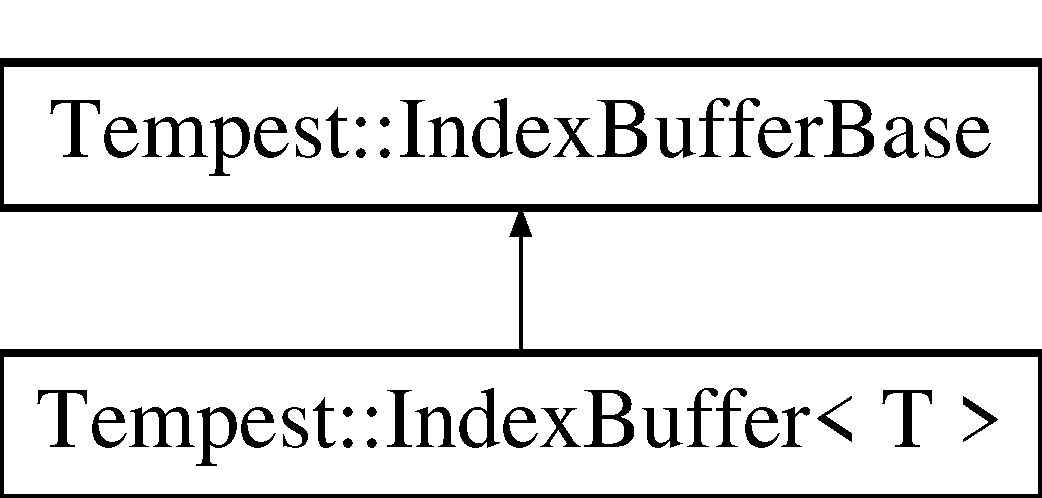
\includegraphics[height=2.000000cm]{class_tempest_1_1_index_buffer}
\end{center}
\end{figure}
\subsection*{Public Types}
\begin{DoxyCompactItemize}
\item 
\hypertarget{class_tempest_1_1_index_buffer_a33db416c299b4856313257f6bde12c54}{typedef \hyperlink{class_tempest_1_1_abstract_holder}{Abstract\+Holder}\\*
$<$ \hyperlink{class_tempest_1_1_index_buffer_base}{Tempest\+::\+Index\+Buffer\+Base}, \\*
Abstract\+A\+P\+I\+::\+Index\+Buffer $>$ {\bfseries Holder}}\label{class_tempest_1_1_index_buffer_a33db416c299b4856313257f6bde12c54}

\end{DoxyCompactItemize}
\subsection*{Public Member Functions}
\begin{DoxyCompactItemize}
\item 
\hypertarget{class_tempest_1_1_index_buffer_a29ac96842a80279fb6da6048fe3670f3}{{\bfseries Index\+Buffer} (\hyperlink{class_tempest_1_1_abstract_holder}{Holder} \&h, int s)}\label{class_tempest_1_1_index_buffer_a29ac96842a80279fb6da6048fe3670f3}

\item 
\hypertarget{class_tempest_1_1_index_buffer_a31345f3ccdc7e29d83c4b86acebada46}{int {\bfseries size} () const }\label{class_tempest_1_1_index_buffer_a31345f3ccdc7e29d83c4b86acebada46}

\item 
\hypertarget{class_tempest_1_1_index_buffer_aba033124166a5ccc2c356cf0a7321ab1}{\hyperlink{class_tempest_1_1_index_buffer}{Index\+Buffer}$<$ Index $>$ {\bfseries slice} (int first, int size) const }\label{class_tempest_1_1_index_buffer_aba033124166a5ccc2c356cf0a7321ab1}

\item 
\hypertarget{class_tempest_1_1_index_buffer_a877a05d3a5ea8d6e46b906ed162e6578}{\hyperlink{class_tempest_1_1_index_buffer}{Index\+Buffer}$<$ Index $>$ {\bfseries slice} (int first) const }\label{class_tempest_1_1_index_buffer_a877a05d3a5ea8d6e46b906ed162e6578}

\item 
\hypertarget{class_tempest_1_1_index_buffer_a6ddf1c05eead33d4e7fb03298cd548dd}{{\footnotesize template$<$class I $>$ }\\void {\bfseries get} (I begin, I end, int b) const }\label{class_tempest_1_1_index_buffer_a6ddf1c05eead33d4e7fb03298cd548dd}

\item 
\hypertarget{class_tempest_1_1_index_buffer_a6fbef5af35ece39d98028a1b33ab2e21}{size\+\_\+t {\bfseries handle} () const }\label{class_tempest_1_1_index_buffer_a6fbef5af35ece39d98028a1b33ab2e21}

\end{DoxyCompactItemize}
\subsection*{Friends}
\begin{DoxyCompactItemize}
\item 
\hypertarget{class_tempest_1_1_index_buffer_a520fa05e0bf58785da428f7a0241eee2}{class {\bfseries Device}}\label{class_tempest_1_1_index_buffer_a520fa05e0bf58785da428f7a0241eee2}

\item 
\hypertarget{class_tempest_1_1_index_buffer_a931bc0ce4135d164772c0f084bac3f11}{class {\bfseries Index\+Buffer\+Holder}}\label{class_tempest_1_1_index_buffer_a931bc0ce4135d164772c0f084bac3f11}

\end{DoxyCompactItemize}


The documentation for this class was generated from the following files\+:\begin{DoxyCompactItemize}
\item 
core/device.\+h\item 
core/wrappers/indexbuffer.\+h\end{DoxyCompactItemize}

\hypertarget{class_tempest_1_1_index_buffer_base}{\section{Tempest\+:\+:Index\+Buffer\+Base Class Reference}
\label{class_tempest_1_1_index_buffer_base}\index{Tempest\+::\+Index\+Buffer\+Base@{Tempest\+::\+Index\+Buffer\+Base}}
}
Inheritance diagram for Tempest\+:\+:Index\+Buffer\+Base\+:\begin{figure}[H]
\begin{center}
\leavevmode
\includegraphics[height=2.000000cm]{class_tempest_1_1_index_buffer_base}
\end{center}
\end{figure}


The documentation for this class was generated from the following file\+:\begin{DoxyCompactItemize}
\item 
core/wrappers/indexbuffer.\+h\end{DoxyCompactItemize}

\hypertarget{class_tempest_1_1_index_buffer_holder}{\section{Tempest\+:\+:Index\+Buffer\+Holder Class Reference}
\label{class_tempest_1_1_index_buffer_holder}\index{Tempest\+::\+Index\+Buffer\+Holder@{Tempest\+::\+Index\+Buffer\+Holder}}
}
Inheritance diagram for Tempest\+:\+:Index\+Buffer\+Holder\+:\begin{figure}[H]
\begin{center}
\leavevmode
\includegraphics[height=5.000000cm]{class_tempest_1_1_index_buffer_holder}
\end{center}
\end{figure}
\subsection*{Classes}
\begin{DoxyCompactItemize}
\item 
struct \hyperlink{struct_index_buffer_holder_1_1_data}{Data}
\end{DoxyCompactItemize}
\subsection*{Public Types}
\begin{DoxyCompactItemize}
\item 
\hypertarget{class_tempest_1_1_index_buffer_holder_aa191f80192940101f77630e0b8e2272d}{typedef \hyperlink{class_tempest_1_1_abstract_holder}{Abstract\+Holder}\\*
$<$ \hyperlink{class_tempest_1_1_index_buffer_base}{Tempest\+::\+Index\+Buffer\+Base}, \\*
Abstract\+A\+P\+I\+::\+Index\+Buffer $>$ {\bfseries Base\+Type}}\label{class_tempest_1_1_index_buffer_holder_aa191f80192940101f77630e0b8e2272d}

\end{DoxyCompactItemize}
\subsection*{Public Member Functions}
\begin{DoxyCompactItemize}
\item 
\hypertarget{class_tempest_1_1_index_buffer_holder_a64b7d85d2ce75bdcb01e6548c6b7a883}{{\bfseries Index\+Buffer\+Holder} (\hyperlink{class_tempest_1_1_device}{Device} \&d)}\label{class_tempest_1_1_index_buffer_holder_a64b7d85d2ce75bdcb01e6548c6b7a883}

\item 
\hypertarget{class_tempest_1_1_index_buffer_holder_a70c5e61afb62de78922db86fd55f80af}{{\footnotesize template$<$class Index $>$ }\\\hyperlink{class_tempest_1_1_index_buffer}{Index\+Buffer}$<$ Index $>$ {\bfseries load} (const Index v\mbox{[}$\,$\mbox{]}, int count, Abstract\+A\+P\+I\+::\+Buffer\+Flag flg=Abstract\+A\+P\+I\+::\+B\+F\+\_\+\+No\+Flags)}\label{class_tempest_1_1_index_buffer_holder_a70c5e61afb62de78922db86fd55f80af}

\item 
\hypertarget{class_tempest_1_1_index_buffer_holder_a7c5569966fea598b70aafcca93475733}{{\footnotesize template$<$class Index $>$ }\\\hyperlink{class_tempest_1_1_index_buffer}{Index\+Buffer}$<$ Index $>$ {\bfseries load} (const std\+::vector$<$ Index $>$ \&ibo, Abstract\+A\+P\+I\+::\+Buffer\+Flag flg=Abstract\+A\+P\+I\+::\+B\+F\+\_\+\+No\+Flags)}\label{class_tempest_1_1_index_buffer_holder_a7c5569966fea598b70aafcca93475733}

\end{DoxyCompactItemize}
\subsection*{Protected Types}
\begin{DoxyCompactItemize}
\item 
\hypertarget{class_tempest_1_1_index_buffer_holder_aa77ffbcc7d92ae0b5b469394120be7e8}{typedef Abstract\+A\+P\+I\+::\+Index\+Buffer {\bfseries Descriptor\+Type}}\label{class_tempest_1_1_index_buffer_holder_aa77ffbcc7d92ae0b5b469394120be7e8}

\end{DoxyCompactItemize}
\subsection*{Protected Member Functions}
\begin{DoxyCompactItemize}
\item 
\hypertarget{class_tempest_1_1_index_buffer_holder_a04358f769c214ff88e17d15ef7ec6126}{virtual void {\bfseries create\+Object} (Abstract\+A\+P\+I\+::\+Index\+Buffer $\ast$\&t, const char $\ast$src, int size, int vsize, Abstract\+A\+P\+I\+::\+Buffer\+Flag flg)}\label{class_tempest_1_1_index_buffer_holder_a04358f769c214ff88e17d15ef7ec6126}

\item 
\hypertarget{class_tempest_1_1_index_buffer_holder_a60f3221d9d2290d96b6d8a01c5cf7425}{virtual void {\bfseries delete\+Object} (Abstract\+A\+P\+I\+::\+Index\+Buffer $\ast$t)}\label{class_tempest_1_1_index_buffer_holder_a60f3221d9d2290d96b6d8a01c5cf7425}

\item 
\hypertarget{class_tempest_1_1_index_buffer_holder_a0237328b430e24d22578c233f4e3c3ed}{virtual Abstract\+A\+P\+I\+::\+Index\+Buffer $\ast$ {\bfseries alloc\+Buffer} (size\+\_\+t size, size\+\_\+t vsize, const void $\ast$src, Abstract\+A\+P\+I\+::\+Buffer\+Flag flg=Abstract\+A\+P\+I\+::\+B\+F\+\_\+\+No\+Flags)}\label{class_tempest_1_1_index_buffer_holder_a0237328b430e24d22578c233f4e3c3ed}

\item 
\hypertarget{class_tempest_1_1_index_buffer_holder_a2258b8b0787ef97f864c2e7af2f224b5}{virtual Abstract\+A\+P\+I\+::\+Index\+Buffer $\ast$ {\bfseries alloc\+Buffer} (size\+\_\+t size, size\+\_\+t vsize, const void $\ast$src, Abstract\+A\+P\+I\+::\+Buffer\+Usage u, Abstract\+A\+P\+I\+::\+Buffer\+Flag flg=Abstract\+A\+P\+I\+::\+B\+F\+\_\+\+No\+Flags)}\label{class_tempest_1_1_index_buffer_holder_a2258b8b0787ef97f864c2e7af2f224b5}

\item 
\hypertarget{class_tempest_1_1_index_buffer_holder_a0fb8a559f63193f30f3ee196de58884f}{virtual void {\bfseries reset} (Abstract\+A\+P\+I\+::\+Index\+Buffer $\ast$t)}\label{class_tempest_1_1_index_buffer_holder_a0fb8a559f63193f30f3ee196de58884f}

\item 
\hypertarget{class_tempest_1_1_index_buffer_holder_a85dba0dd86d7c85725df7365d99147fb}{virtual Abstract\+A\+P\+I\+::\+Index\+Buffer $\ast$ {\bfseries restore} (Abstract\+A\+P\+I\+::\+Index\+Buffer $\ast$t)}\label{class_tempest_1_1_index_buffer_holder_a85dba0dd86d7c85725df7365d99147fb}

\item 
\hypertarget{class_tempest_1_1_index_buffer_holder_aad5532e23380d755662af7771d1ce3ff}{virtual Abstract\+A\+P\+I\+::\+Index\+Buffer $\ast$ {\bfseries copy} (Abstract\+A\+P\+I\+::\+Index\+Buffer $\ast$t)}\label{class_tempest_1_1_index_buffer_holder_aad5532e23380d755662af7771d1ce3ff}

\item 
\hypertarget{class_tempest_1_1_index_buffer_holder_aba7c1537f1bed08dd82fc98e228246c9}{char $\ast$ {\bfseries lock\+Buffer} (Abstract\+A\+P\+I\+::\+Index\+Buffer $\ast$t, int b, int sz)}\label{class_tempest_1_1_index_buffer_holder_aba7c1537f1bed08dd82fc98e228246c9}

\item 
\hypertarget{class_tempest_1_1_index_buffer_holder_a2ba8060265f44c644db586814363ea7d}{void {\bfseries unlock\+Buffer} (Abstract\+A\+P\+I\+::\+Index\+Buffer $\ast$t)}\label{class_tempest_1_1_index_buffer_holder_a2ba8060265f44c644db586814363ea7d}

\end{DoxyCompactItemize}
\subsection*{Friends}
\begin{DoxyCompactItemize}
\item 
\hypertarget{class_tempest_1_1_index_buffer_holder_a96a587d509460c7d76a779193a51afdc}{class {\bfseries Index\+Buffer\+Base}}\label{class_tempest_1_1_index_buffer_holder_a96a587d509460c7d76a779193a51afdc}

\item 
\hypertarget{class_tempest_1_1_index_buffer_holder_a391602b00b2303b580c0546f1d0e1c4e}{{\footnotesize template$<$class I $>$ }\\class {\bfseries Index\+Buffer}}\label{class_tempest_1_1_index_buffer_holder_a391602b00b2303b580c0546f1d0e1c4e}

\end{DoxyCompactItemize}
\subsection*{Additional Inherited Members}


\subsection{Detailed Description}
\begin{Desc}
\item[Examples\+: ]\par
\hyperlink{_cube_2mainwindow_8h-example}{Cube/mainwindow.\+h}, and \hyperlink{_painting2d_2mainwindow_8h-example}{Painting2d/mainwindow.\+h}.\end{Desc}


The documentation for this class was generated from the following files\+:\begin{DoxyCompactItemize}
\item 
data\+Control/indexbufferholder.\+h\item 
data\+Control/indexbufferholder.\+cpp\end{DoxyCompactItemize}

\hypertarget{struct_tempest_1_1_abstract_texture_1_1_input_format}{\section{Tempest\+:\+:Abstract\+Texture\+:\+:Input\+Format Struct Reference}
\label{struct_tempest_1_1_abstract_texture_1_1_input_format}\index{Tempest\+::\+Abstract\+Texture\+::\+Input\+Format@{Tempest\+::\+Abstract\+Texture\+::\+Input\+Format}}
}


{\ttfamily \#include $<$abstracttexture.\+h$>$}

\subsection*{Public Types}
\begin{DoxyCompactItemize}
\item 
\hypertarget{struct_tempest_1_1_abstract_texture_1_1_input_format_a76bada4dfe78209969b1e3e232e34279}{enum \hyperlink{struct_tempest_1_1_abstract_texture_1_1_input_format_a76bada4dfe78209969b1e3e232e34279}{Type} \{ \\*
{\bfseries Luminance8}, 
{\bfseries R\+G\+B8}, 
{\bfseries R\+G\+B\+A8}, 
{\bfseries Depth}, 
\\*
{\bfseries Count}
 \}}\label{struct_tempest_1_1_abstract_texture_1_1_input_format_a76bada4dfe78209969b1e3e232e34279}

\begin{DoxyCompactList}\small\item\em Формат, в которром текстура хранится в ОЗУ. \end{DoxyCompactList}\end{DoxyCompactItemize}


\subsection{Detailed Description}
Формат, в которром текстура хранится в ОЗУ. При загрузке тексели будут преобразованны к Tempest\+::\+I\+Texture\+::\+Format. 

The documentation for this struct was generated from the following file\+:\begin{DoxyCompactItemize}
\item 
core/wrappers/abstracttexture.\+h\end{DoxyCompactItemize}

\hypertarget{struct_tempest_1_1_jpeg_codec}{\section{Tempest\+:\+:Jpeg\+Codec Struct Reference}
\label{struct_tempest_1_1_jpeg_codec}\index{Tempest\+::\+Jpeg\+Codec@{Tempest\+::\+Jpeg\+Codec}}
}
Inheritance diagram for Tempest\+:\+:Jpeg\+Codec\+:\begin{figure}[H]
\begin{center}
\leavevmode
\includegraphics[height=2.000000cm]{struct_tempest_1_1_jpeg_codec}
\end{center}
\end{figure}
\subsection*{Classes}
\begin{DoxyCompactItemize}
\item 
struct \hyperlink{struct_tempest_1_1_jpeg_codec_1_1compress}{compress}
\item 
struct \hyperlink{struct_tempest_1_1_jpeg_codec_1_1_jpeg_stream}{Jpeg\+Stream}
\end{DoxyCompactItemize}
\subsection*{Public Member Functions}
\begin{DoxyCompactItemize}
\item 
\hypertarget{struct_tempest_1_1_jpeg_codec_a58a803d04ebdfae1f9ffaa6878e440ff}{void {\bfseries make\+\_\+stream} (jpeg\+\_\+decompress\+\_\+struct $\ast$cinfo, \hyperlink{class_tempest_1_1_i_device}{I\+Device} $\ast$in)}\label{struct_tempest_1_1_jpeg_codec_a58a803d04ebdfae1f9ffaa6878e440ff}

\item 
\hypertarget{struct_tempest_1_1_jpeg_codec_a4fe73b181a7a014c2999d8394571bcb8}{bool {\bfseries load} (\hyperlink{class_tempest_1_1_i_device}{I\+Device} \&d, \hyperlink{struct_tempest_1_1_pixmap_1_1_img_info}{Img\+Info} \&info, std\+::vector$<$ unsigned char $>$ \&out)}\label{struct_tempest_1_1_jpeg_codec_a4fe73b181a7a014c2999d8394571bcb8}

\end{DoxyCompactItemize}
\subsection*{Static Public Member Functions}
\begin{DoxyCompactItemize}
\item 
\hypertarget{struct_tempest_1_1_jpeg_codec_a1e43c366f23e90a3000e0e801b0eb7ed}{static void {\bfseries init\+\_\+source} (j\+\_\+decompress\+\_\+ptr)}\label{struct_tempest_1_1_jpeg_codec_a1e43c366f23e90a3000e0e801b0eb7ed}

\item 
\hypertarget{struct_tempest_1_1_jpeg_codec_a3bf45c99bb953cd081873a9da4c61361}{static boolean {\bfseries fill\+\_\+buffer} (j\+\_\+decompress\+\_\+ptr cinfo)}\label{struct_tempest_1_1_jpeg_codec_a3bf45c99bb953cd081873a9da4c61361}

\item 
\hypertarget{struct_tempest_1_1_jpeg_codec_aaa23356b0bed05fbf73fccf5c188b9c5}{static void {\bfseries skip} (j\+\_\+decompress\+\_\+ptr cinfo, long count)}\label{struct_tempest_1_1_jpeg_codec_aaa23356b0bed05fbf73fccf5c188b9c5}

\item 
\hypertarget{struct_tempest_1_1_jpeg_codec_ac30f117c65fd781b610b310424455807}{static void {\bfseries term} (j\+\_\+decompress\+\_\+ptr)}\label{struct_tempest_1_1_jpeg_codec_ac30f117c65fd781b610b310424455807}

\item 
\hypertarget{struct_tempest_1_1_jpeg_codec_ae85cc7c36ce5f288d9d5b521138dfbaf}{static void {\bfseries handle\+Lib\+Jpeg\+Fatal\+Error} (j\+\_\+common\+\_\+ptr)}\label{struct_tempest_1_1_jpeg_codec_ae85cc7c36ce5f288d9d5b521138dfbaf}

\end{DoxyCompactItemize}
\subsection*{Additional Inherited Members}


The documentation for this struct was generated from the following file\+:\begin{DoxyCompactItemize}
\item 
core/imagecodec.\+cpp\end{DoxyCompactItemize}

\hypertarget{struct_tempest_1_1_jpeg_codec_1_1_jpeg_stream}{\section{Tempest\+:\+:Jpeg\+Codec\+:\+:Jpeg\+Stream Struct Reference}
\label{struct_tempest_1_1_jpeg_codec_1_1_jpeg_stream}\index{Tempest\+::\+Jpeg\+Codec\+::\+Jpeg\+Stream@{Tempest\+::\+Jpeg\+Codec\+::\+Jpeg\+Stream}}
}
\subsection*{Public Attributes}
\begin{DoxyCompactItemize}
\item 
\hypertarget{struct_tempest_1_1_jpeg_codec_1_1_jpeg_stream_ab62c802c7468baf27d63abe5d14738f6}{jpeg\+\_\+source\+\_\+mgr {\bfseries pub}}\label{struct_tempest_1_1_jpeg_codec_1_1_jpeg_stream_ab62c802c7468baf27d63abe5d14738f6}

\item 
\hypertarget{struct_tempest_1_1_jpeg_codec_1_1_jpeg_stream_acdc0dacdc3f928f07bf1a3f1865a1df5}{\hyperlink{class_tempest_1_1_i_device}{I\+Device} $\ast$ {\bfseries stream}}\label{struct_tempest_1_1_jpeg_codec_1_1_jpeg_stream_acdc0dacdc3f928f07bf1a3f1865a1df5}

\item 
\hypertarget{struct_tempest_1_1_jpeg_codec_1_1_jpeg_stream_a10c4f325d983b0d3b180119e6a8d0341}{unsigned char {\bfseries buffer} \mbox{[}buffer\+Size\mbox{]}}\label{struct_tempest_1_1_jpeg_codec_1_1_jpeg_stream_a10c4f325d983b0d3b180119e6a8d0341}

\end{DoxyCompactItemize}
\subsection*{Static Public Attributes}
\begin{DoxyCompactItemize}
\item 
\hypertarget{struct_tempest_1_1_jpeg_codec_1_1_jpeg_stream_a7ee395575c44f304ca584c421823ccc9}{static const size\+\_\+t {\bfseries buffer\+Size} = 4096}\label{struct_tempest_1_1_jpeg_codec_1_1_jpeg_stream_a7ee395575c44f304ca584c421823ccc9}

\end{DoxyCompactItemize}


The documentation for this struct was generated from the following file\+:\begin{DoxyCompactItemize}
\item 
core/imagecodec.\+cpp\end{DoxyCompactItemize}

\hypertarget{class_tempest_1_1_key_event}{\section{Tempest\+:\+:Key\+Event Class Reference}
\label{class_tempest_1_1_key_event}\index{Tempest\+::\+Key\+Event@{Tempest\+::\+Key\+Event}}
}
Inheritance diagram for Tempest\+:\+:Key\+Event\+:\begin{figure}[H]
\begin{center}
\leavevmode
\includegraphics[height=2.000000cm]{class_tempest_1_1_key_event}
\end{center}
\end{figure}
\subsection*{Public Member Functions}
\begin{DoxyCompactItemize}
\item 
\hypertarget{class_tempest_1_1_key_event_ade6677a2c594a7f072ccde341db49cb3}{{\bfseries Key\+Event} (Key\+Type k=K\+\_\+\+No\+Key, Type t=Key\+Down)}\label{class_tempest_1_1_key_event_ade6677a2c594a7f072ccde341db49cb3}

\item 
\hypertarget{class_tempest_1_1_key_event_a8292b354fa498765ccb9189ddbdd9fa1}{{\bfseries Key\+Event} (uint32\+\_\+t k, Type t=Key\+Down)}\label{class_tempest_1_1_key_event_a8292b354fa498765ccb9189ddbdd9fa1}

\item 
\hypertarget{class_tempest_1_1_key_event_a5770f060d4356d820af6f2cb4519905c}{{\bfseries Key\+Event} (Key\+Type k, uint32\+\_\+t k1, Type t=Key\+Down)}\label{class_tempest_1_1_key_event_a5770f060d4356d820af6f2cb4519905c}

\end{DoxyCompactItemize}
\subsection*{Public Attributes}
\begin{DoxyCompactItemize}
\item 
\hypertarget{class_tempest_1_1_key_event_a21fd3762fe4fbe2e6037acedb6ffce4e}{const Key\+Type {\bfseries key}}\label{class_tempest_1_1_key_event_a21fd3762fe4fbe2e6037acedb6ffce4e}

\item 
\hypertarget{class_tempest_1_1_key_event_a68c481e24208dad79104563df95485aa}{const uint32\+\_\+t {\bfseries u16}}\label{class_tempest_1_1_key_event_a68c481e24208dad79104563df95485aa}

\end{DoxyCompactItemize}
\subsection*{Additional Inherited Members}


The documentation for this class was generated from the following file\+:\begin{DoxyCompactItemize}
\item 
ui/event.\+h\end{DoxyCompactItemize}

\hypertarget{class_tempest_1_1_layout}{\section{Tempest\+:\+:Layout Class Reference}
\label{class_tempest_1_1_layout}\index{Tempest\+::\+Layout@{Tempest\+::\+Layout}}
}


The \hyperlink{class_tempest_1_1_layout}{Layout} class is the base class of ui-\/geometry managers.  




{\ttfamily \#include $<$layout.\+h$>$}

Inheritance diagram for Tempest\+:\+:Layout\+:\begin{figure}[H]
\begin{center}
\leavevmode
\includegraphics[height=2.000000cm]{class_tempest_1_1_layout}
\end{center}
\end{figure}
\subsection*{Public Member Functions}
\begin{DoxyCompactItemize}
\item 
\hypertarget{class_tempest_1_1_layout_a29d7b2b1816bf008ba9ea3eda2725fda}{\hyperlink{class_tempest_1_1_widget}{Widget} $\ast$ {\bfseries owner} ()}\label{class_tempest_1_1_layout_a29d7b2b1816bf008ba9ea3eda2725fda}

\item 
\hypertarget{class_tempest_1_1_layout_a444a047bb69354ec6f76264a9e31e04c}{const \hyperlink{class_tempest_1_1_widget}{Widget} $\ast$ {\bfseries owner} () const }\label{class_tempest_1_1_layout_a444a047bb69354ec6f76264a9e31e04c}

\item 
\hypertarget{class_tempest_1_1_layout_aa3b2af0f1f32ed681e40215e3f48b283}{void {\bfseries add} (\hyperlink{class_tempest_1_1_widget}{Widget} $\ast$widget)}\label{class_tempest_1_1_layout_aa3b2af0f1f32ed681e40215e3f48b283}

\item 
\hypertarget{class_tempest_1_1_layout_a2e30bb81cf8c464e6f1bda11fee2fdf4}{void {\bfseries del} (\hyperlink{class_tempest_1_1_widget}{Widget} $\ast$widget)}\label{class_tempest_1_1_layout_a2e30bb81cf8c464e6f1bda11fee2fdf4}

\item 
\hypertarget{class_tempest_1_1_layout_a3b479d59cef4b31228d0ae0e7f446d07}{void {\bfseries remove\+All} ()}\label{class_tempest_1_1_layout_a3b479d59cef4b31228d0ae0e7f446d07}

\item 
\hypertarget{class_tempest_1_1_layout_a8604c30ec4d0192d7535d0411f89b4fc}{\hyperlink{class_tempest_1_1_widget}{Widget} $\ast$ {\bfseries take} (\hyperlink{class_tempest_1_1_widget}{Widget} $\ast$widget)}\label{class_tempest_1_1_layout_a8604c30ec4d0192d7535d0411f89b4fc}

\item 
\hypertarget{class_tempest_1_1_layout_a4819902514d0731c00f33e09892d0f98}{const std\+::vector$<$ \hyperlink{class_tempest_1_1_widget}{Widget} $\ast$ $>$ \& {\bfseries widgets} ()}\label{class_tempest_1_1_layout_a4819902514d0731c00f33e09892d0f98}

\item 
\hypertarget{class_tempest_1_1_layout_a90f8470da068f33f79bdd8aab15944ad}{virtual void {\bfseries apply\+Layout} ()}\label{class_tempest_1_1_layout_a90f8470da068f33f79bdd8aab15944ad}

\item 
\hypertarget{class_tempest_1_1_layout_af418c6fbe4f82e1a3a14c596cf50b895}{void {\bfseries set\+Spacing} (int s)}\label{class_tempest_1_1_layout_af418c6fbe4f82e1a3a14c596cf50b895}

\item 
\hypertarget{class_tempest_1_1_layout_a5dd98a7f5bd3b4bb2eea2c1e022c9598}{int {\bfseries spacing} () const }\label{class_tempest_1_1_layout_a5dd98a7f5bd3b4bb2eea2c1e022c9598}

\item 
\hypertarget{class_tempest_1_1_layout_a605f2680fb9ddd005805da1d212be1f1}{void {\bfseries set\+Margin} (const \hyperlink{struct_tempest_1_1_margin}{Margin} \&m)}\label{class_tempest_1_1_layout_a605f2680fb9ddd005805da1d212be1f1}

\item 
\hypertarget{class_tempest_1_1_layout_a9ebf5d9fa194a2b13dc2a228ba6126c0}{void {\bfseries set\+Margin} (int l, int r, int t, int b)}\label{class_tempest_1_1_layout_a9ebf5d9fa194a2b13dc2a228ba6126c0}

\item 
\hypertarget{class_tempest_1_1_layout_a1d099fd11854fdfbdbcce0317a8bdc3a}{const \hyperlink{struct_tempest_1_1_margin}{Margin} \& {\bfseries margin} () const }\label{class_tempest_1_1_layout_a1d099fd11854fdfbdbcce0317a8bdc3a}

\end{DoxyCompactItemize}
\subsection*{Static Protected Member Functions}
\begin{DoxyCompactItemize}
\item 
\hypertarget{class_tempest_1_1_layout_a2859f142bec996dcd51100d57cfb3213}{static void {\bfseries place\+In} (\hyperlink{class_tempest_1_1_widget}{Widget} $\ast$wx, int x, int y, int w, int h)}\label{class_tempest_1_1_layout_a2859f142bec996dcd51100d57cfb3213}

\item 
\hypertarget{class_tempest_1_1_layout_a8a6fe7f26e1fe6d8509a2a9c0a1ae438}{static void {\bfseries place\+In} (\hyperlink{class_tempest_1_1_widget}{Widget} $\ast$wx, const \hyperlink{struct_tempest_1_1_rect}{Rect} \&r)}\label{class_tempest_1_1_layout_a8a6fe7f26e1fe6d8509a2a9c0a1ae438}

\item 
\hypertarget{class_tempest_1_1_layout_af03db7399995fda263a98cdc68eee76a}{static \hyperlink{struct_tempest_1_1_size}{Size} {\bfseries size\+Hint} (\hyperlink{class_tempest_1_1_widget}{Widget} $\ast$wx)}\label{class_tempest_1_1_layout_af03db7399995fda263a98cdc68eee76a}

\end{DoxyCompactItemize}
\subsection*{Friends}
\begin{DoxyCompactItemize}
\item 
\hypertarget{class_tempest_1_1_layout_a29fa75ce3911bef8c5f4414f6f0242b8}{class {\bfseries Widget}}\label{class_tempest_1_1_layout_a29fa75ce3911bef8c5f4414f6f0242b8}

\end{DoxyCompactItemize}


\subsection{Detailed Description}
The \hyperlink{class_tempest_1_1_layout}{Layout} class is the base class of ui-\/geometry managers. 

The documentation for this class was generated from the following files\+:\begin{DoxyCompactItemize}
\item 
ui/layout.\+h\item 
ui/layout.\+cpp\end{DoxyCompactItemize}

\hypertarget{struct_index_buffer_holder_1_1_data_1_1_l_d_data}{\section{Tempest\+:\+:Index\+Buffer\+Holder\+:\+:Data\+:\+:L\+D\+Data Struct Reference}
\label{struct_index_buffer_holder_1_1_data_1_1_l_d_data}\index{Tempest\+::\+Index\+Buffer\+Holder\+::\+Data\+::\+L\+D\+Data@{Tempest\+::\+Index\+Buffer\+Holder\+::\+Data\+::\+L\+D\+Data}}
}
\subsection*{Public Attributes}
\begin{DoxyCompactItemize}
\item 
\hypertarget{struct_index_buffer_holder_1_1_data_1_1_l_d_data_a5092ebbb9cd8c03660db66977dcdc64a}{int {\bfseries vsize}}\label{struct_index_buffer_holder_1_1_data_1_1_l_d_data_a5092ebbb9cd8c03660db66977dcdc64a}

\item 
\hypertarget{struct_index_buffer_holder_1_1_data_1_1_l_d_data_a91a1a0b289e3aed0f175eff7a2904c2b}{int {\bfseries size}}\label{struct_index_buffer_holder_1_1_data_1_1_l_d_data_a91a1a0b289e3aed0f175eff7a2904c2b}

\item 
\hypertarget{struct_index_buffer_holder_1_1_data_1_1_l_d_data_af5fe2f9a4852915c9f4c2bdb90d39deb}{int {\bfseries lock\+Begin}}\label{struct_index_buffer_holder_1_1_data_1_1_l_d_data_af5fe2f9a4852915c9f4c2bdb90d39deb}

\item 
\hypertarget{struct_index_buffer_holder_1_1_data_1_1_l_d_data_a63af362e39607a1c70abb22557dc5d81}{int {\bfseries lock\+Size}}\label{struct_index_buffer_holder_1_1_data_1_1_l_d_data_a63af362e39607a1c70abb22557dc5d81}

\item 
\hypertarget{struct_index_buffer_holder_1_1_data_1_1_l_d_data_a4bc7a7d52d57d132b11bd187b010e0ed}{std\+::vector$<$ char $>$ {\bfseries data}}\label{struct_index_buffer_holder_1_1_data_1_1_l_d_data_a4bc7a7d52d57d132b11bd187b010e0ed}

\end{DoxyCompactItemize}


The documentation for this struct was generated from the following file\+:\begin{DoxyCompactItemize}
\item 
data\+Control/indexbufferholder.\+cpp\end{DoxyCompactItemize}

\hypertarget{struct_vertex_buffer_holder_1_1_data_1_1_l_d_data}{\section{Tempest\+:\+:Vertex\+Buffer\+Holder\+:\+:Data\+:\+:L\+D\+Data Struct Reference}
\label{struct_vertex_buffer_holder_1_1_data_1_1_l_d_data}\index{Tempest\+::\+Vertex\+Buffer\+Holder\+::\+Data\+::\+L\+D\+Data@{Tempest\+::\+Vertex\+Buffer\+Holder\+::\+Data\+::\+L\+D\+Data}}
}
\subsection*{Public Attributes}
\begin{DoxyCompactItemize}
\item 
\hypertarget{struct_vertex_buffer_holder_1_1_data_1_1_l_d_data_ad7e6e5af10a1fb10dfb284564f594377}{int {\bfseries vsize}}\label{struct_vertex_buffer_holder_1_1_data_1_1_l_d_data_ad7e6e5af10a1fb10dfb284564f594377}

\item 
\hypertarget{struct_vertex_buffer_holder_1_1_data_1_1_l_d_data_a926f0e24dba8b7f6c2dfa97e6fcc3e20}{int {\bfseries size}}\label{struct_vertex_buffer_holder_1_1_data_1_1_l_d_data_a926f0e24dba8b7f6c2dfa97e6fcc3e20}

\item 
\hypertarget{struct_vertex_buffer_holder_1_1_data_1_1_l_d_data_a79f249c95479d0508204cd8839911462}{int {\bfseries lock\+Begin}}\label{struct_vertex_buffer_holder_1_1_data_1_1_l_d_data_a79f249c95479d0508204cd8839911462}

\item 
\hypertarget{struct_vertex_buffer_holder_1_1_data_1_1_l_d_data_aa1e1ab333d6d23842e29066fd5f0b272}{int {\bfseries lock\+Size}}\label{struct_vertex_buffer_holder_1_1_data_1_1_l_d_data_aa1e1ab333d6d23842e29066fd5f0b272}

\item 
\hypertarget{struct_vertex_buffer_holder_1_1_data_1_1_l_d_data_aa999d8cad8eabd8df1c13c3eaecccf56}{std\+::vector$<$ char $>$ {\bfseries data}}\label{struct_vertex_buffer_holder_1_1_data_1_1_l_d_data_aa999d8cad8eabd8df1c13c3eaecccf56}

\end{DoxyCompactItemize}


The documentation for this struct was generated from the following file\+:\begin{DoxyCompactItemize}
\item 
data\+Control/vertexbufferholder.\+cpp\end{DoxyCompactItemize}

\hypertarget{struct_tempest_1_1_font_element_1_1_letter}{\section{Tempest\+:\+:Font\+Element\+:\+:Letter Struct Reference}
\label{struct_tempest_1_1_font_element_1_1_letter}\index{Tempest\+::\+Font\+Element\+::\+Letter@{Tempest\+::\+Font\+Element\+::\+Letter}}
}
\subsection*{Public Attributes}
\begin{DoxyCompactItemize}
\item 
\hypertarget{struct_tempest_1_1_font_element_1_1_letter_ac12348263fa0f19dd21740c2f8a1d6dc}{\hyperlink{class_tempest_1_1_sprite}{Tempest\+::\+Sprite} {\bfseries surf}}\label{struct_tempest_1_1_font_element_1_1_letter_ac12348263fa0f19dd21740c2f8a1d6dc}

\item 
\hypertarget{struct_tempest_1_1_font_element_1_1_letter_a1d750a9243d7b789a120dd2e47d4e92c}{\hyperlink{struct_tempest_1_1_size}{Tempest\+::\+Size} {\bfseries size}}\label{struct_tempest_1_1_font_element_1_1_letter_a1d750a9243d7b789a120dd2e47d4e92c}

\item 
\hypertarget{struct_tempest_1_1_font_element_1_1_letter_ad8d38c1fdf898e1086170ed1b1c13219}{\hyperlink{struct_tempest_1_1_point}{Tempest\+::\+Point} {\bfseries dpos}}\label{struct_tempest_1_1_font_element_1_1_letter_ad8d38c1fdf898e1086170ed1b1c13219}

\item 
\hypertarget{struct_tempest_1_1_font_element_1_1_letter_a628edad2f210cc4a8f1e09b7f459adab}{\hyperlink{struct_tempest_1_1_point}{Tempest\+::\+Point} {\bfseries advance}}\label{struct_tempest_1_1_font_element_1_1_letter_a628edad2f210cc4a8f1e09b7f459adab}

\end{DoxyCompactItemize}


The documentation for this struct was generated from the following file\+:\begin{DoxyCompactItemize}
\item 
2d/font.\+h\end{DoxyCompactItemize}

\hypertarget{struct_tempest_1_1_font_element_1_1_letter_geometry}{\section{Tempest\+:\+:Font\+Element\+:\+:Letter\+Geometry Struct Reference}
\label{struct_tempest_1_1_font_element_1_1_letter_geometry}\index{Tempest\+::\+Font\+Element\+::\+Letter\+Geometry@{Tempest\+::\+Font\+Element\+::\+Letter\+Geometry}}
}
\subsection*{Public Attributes}
\begin{DoxyCompactItemize}
\item 
\hypertarget{struct_tempest_1_1_font_element_1_1_letter_geometry_a0c5fbd0081070532f3becaf600c4efc6}{\hyperlink{struct_tempest_1_1_size}{Tempest\+::\+Size} {\bfseries size}}\label{struct_tempest_1_1_font_element_1_1_letter_geometry_a0c5fbd0081070532f3becaf600c4efc6}

\item 
\hypertarget{struct_tempest_1_1_font_element_1_1_letter_geometry_af82814ba2b9ab2a1dcb0e093abb9a4e3}{\hyperlink{struct_tempest_1_1_point}{Tempest\+::\+Point} {\bfseries dpos}}\label{struct_tempest_1_1_font_element_1_1_letter_geometry_af82814ba2b9ab2a1dcb0e093abb9a4e3}

\item 
\hypertarget{struct_tempest_1_1_font_element_1_1_letter_geometry_a156ef7720039e8af14e8d395779e3e2c}{\hyperlink{struct_tempest_1_1_point}{Tempest\+::\+Point} {\bfseries advance}}\label{struct_tempest_1_1_font_element_1_1_letter_geometry_a156ef7720039e8af14e8d395779e3e2c}

\end{DoxyCompactItemize}


The documentation for this struct was generated from the following file\+:\begin{DoxyCompactItemize}
\item 
2d/font.\+h\end{DoxyCompactItemize}

\hypertarget{class_tempest_1_1_light_collection}{\section{Tempest\+:\+:Light\+Collection Class Reference}
\label{class_tempest_1_1_light_collection}\index{Tempest\+::\+Light\+Collection@{Tempest\+::\+Light\+Collection}}
}
Inheritance diagram for Tempest\+:\+:Light\+Collection\+:\begin{figure}[H]
\begin{center}
\leavevmode
\includegraphics[height=2.000000cm]{class_tempest_1_1_light_collection}
\end{center}
\end{figure}
\subsection*{Classes}
\begin{DoxyCompactItemize}
\item 
class \hyperlink{class_tempest_1_1_light_collection_1_1_pack}{Pack}
\end{DoxyCompactItemize}
\subsection*{Public Member Functions}
\begin{DoxyCompactItemize}
\item 
\hypertarget{class_tempest_1_1_light_collection_a245b570d14b730765068385bf92f1d31}{virtual const \hyperlink{class_tempest_1_1_abstract_light_collection_1_1_pack}{Direction\+Lights} \& {\bfseries direction} () const }\label{class_tempest_1_1_light_collection_a245b570d14b730765068385bf92f1d31}

\item 
\hypertarget{class_tempest_1_1_light_collection_ac6d10d52dbea6e555cacd038e314e55f}{virtual \hyperlink{class_tempest_1_1_abstract_light_collection_1_1_pack}{Direction\+Lights} \& {\bfseries direction} ()}\label{class_tempest_1_1_light_collection_ac6d10d52dbea6e555cacd038e314e55f}

\end{DoxyCompactItemize}
\subsection*{Additional Inherited Members}


The documentation for this class was generated from the following files\+:\begin{DoxyCompactItemize}
\item 
scene/lightcollection.\+h\item 
scene/lightcollection.\+cpp\end{DoxyCompactItemize}

\hypertarget{class_tempest_1_1_linear_layout}{\section{Tempest\+:\+:Linear\+Layout Class Reference}
\label{class_tempest_1_1_linear_layout}\index{Tempest\+::\+Linear\+Layout@{Tempest\+::\+Linear\+Layout}}
}
Inheritance diagram for Tempest\+:\+:Linear\+Layout\+:\begin{figure}[H]
\begin{center}
\leavevmode
\includegraphics[height=2.000000cm]{class_tempest_1_1_linear_layout}
\end{center}
\end{figure}
\subsection*{Public Member Functions}
\begin{DoxyCompactItemize}
\item 
\hypertarget{class_tempest_1_1_linear_layout_a8c7f0a3f9894f50389e559985be3691a}{{\bfseries Linear\+Layout} (Orientation ori=Vertical)}\label{class_tempest_1_1_linear_layout_a8c7f0a3f9894f50389e559985be3691a}

\item 
\hypertarget{class_tempest_1_1_linear_layout_a4f61198d68d3b6c24280c860ef03ed72}{virtual void {\bfseries apply\+Layout} ()}\label{class_tempest_1_1_linear_layout_a4f61198d68d3b6c24280c860ef03ed72}

\item 
\hypertarget{class_tempest_1_1_linear_layout_a532b381abbc88f33aaa47958eb732524}{Orientation {\bfseries orientation} ()}\label{class_tempest_1_1_linear_layout_a532b381abbc88f33aaa47958eb732524}

\item 
\hypertarget{class_tempest_1_1_linear_layout_aac24f75e5b6e30dfe3df3a3b263d6d0a}{void {\bfseries set\+Orientation} (Orientation ori)}\label{class_tempest_1_1_linear_layout_aac24f75e5b6e30dfe3df3a3b263d6d0a}

\end{DoxyCompactItemize}
\subsection*{Additional Inherited Members}


The documentation for this class was generated from the following files\+:\begin{DoxyCompactItemize}
\item 
ui/layout.\+h\item 
ui/layout.\+cpp\end{DoxyCompactItemize}

\hypertarget{class_tempest_1_1_local_buffer_holder}{\section{Tempest\+:\+:Local\+Buffer\+Holder$<$ Holder $>$ Class Template Reference}
\label{class_tempest_1_1_local_buffer_holder}\index{Tempest\+::\+Local\+Buffer\+Holder$<$ Holder $>$@{Tempest\+::\+Local\+Buffer\+Holder$<$ Holder $>$}}
}
Inheritance diagram for Tempest\+:\+:Local\+Buffer\+Holder$<$ Holder $>$\+:\begin{figure}[H]
\begin{center}
\leavevmode
\includegraphics[height=2.000000cm]{class_tempest_1_1_local_buffer_holder}
\end{center}
\end{figure}
\subsection*{Classes}
\begin{DoxyCompactItemize}
\item 
struct \hyperlink{struct_tempest_1_1_local_buffer_holder_1_1_non_freed}{Non\+Freed}
\item 
struct \hyperlink{struct_tempest_1_1_local_buffer_holder_1_1_non_freed_data}{Non\+Freed\+Data}
\end{DoxyCompactItemize}
\subsection*{Public Member Functions}
\begin{DoxyCompactItemize}
\item 
\hypertarget{class_tempest_1_1_local_buffer_holder_ab71d8be70cf8f8c2cbeaf7ded60df55e}{{\bfseries Local\+Buffer\+Holder} (\hyperlink{class_tempest_1_1_device}{Tempest\+::\+Device} \&d, Abstract\+A\+P\+I\+::\+Buffer\+Usage bu=Abstract\+A\+P\+I\+::\+B\+U\+\_\+\+Dynamic)}\label{class_tempest_1_1_local_buffer_holder_ab71d8be70cf8f8c2cbeaf7ded60df55e}

\item 
\hypertarget{class_tempest_1_1_local_buffer_holder_a626ecb104a46b24089a3dab2ec6b5ffc}{void {\bfseries set\+Max\+Collect\+Iterations} (int c)}\label{class_tempest_1_1_local_buffer_holder_a626ecb104a46b24089a3dab2ec6b5ffc}

\item 
\hypertarget{class_tempest_1_1_local_buffer_holder_ae62471b6f4449b50057b642d18d4abae}{int {\bfseries max\+Collect\+Iterations} () const }\label{class_tempest_1_1_local_buffer_holder_ae62471b6f4449b50057b642d18d4abae}

\item 
\hypertarget{class_tempest_1_1_local_buffer_holder_a0e949509b0523f01bc59e18d2b071362}{void {\bfseries set\+Reserve\+Size} (int sz)}\label{class_tempest_1_1_local_buffer_holder_a0e949509b0523f01bc59e18d2b071362}

\item 
\hypertarget{class_tempest_1_1_local_buffer_holder_a26504685571dbcd32bd77e1980370308}{void {\bfseries set\+Max\+Reserved\+Count} (int s)}\label{class_tempest_1_1_local_buffer_holder_a26504685571dbcd32bd77e1980370308}

\item 
\hypertarget{class_tempest_1_1_local_buffer_holder_aa49488cb2afd3fea872fa053496884c8}{int {\bfseries max\+Reserved\+Count} () const }\label{class_tempest_1_1_local_buffer_holder_aa49488cb2afd3fea872fa053496884c8}

\item 
\hypertarget{class_tempest_1_1_local_buffer_holder_a62a1733530a409420b91649fd38ef242}{void {\bfseries pause\+Collect} (bool p)}\label{class_tempest_1_1_local_buffer_holder_a62a1733530a409420b91649fd38ef242}

\item 
\hypertarget{class_tempest_1_1_local_buffer_holder_a359c6e9b71cf0fa5707a41f3d38e2b78}{bool {\bfseries is\+Collect\+Paused} () const }\label{class_tempest_1_1_local_buffer_holder_a359c6e9b71cf0fa5707a41f3d38e2b78}

\end{DoxyCompactItemize}
\subsection*{Protected Member Functions}
\begin{DoxyCompactItemize}
\item 
\hypertarget{class_tempest_1_1_local_buffer_holder_a5c65e05dc74006a5b79fdc10e29a46be}{virtual void {\bfseries reset} ()}\label{class_tempest_1_1_local_buffer_holder_a5c65e05dc74006a5b79fdc10e29a46be}

\item 
\hypertarget{class_tempest_1_1_local_buffer_holder_a845f41dfc4e2c15d696e30fabe8b52ab}{virtual bool {\bfseries restore} ()}\label{class_tempest_1_1_local_buffer_holder_a845f41dfc4e2c15d696e30fabe8b52ab}

\item 
\hypertarget{class_tempest_1_1_local_buffer_holder_a656a8548e8640563edf24d4e4f18fe50}{virtual void {\bfseries present\+Event} ()}\label{class_tempest_1_1_local_buffer_holder_a656a8548e8640563edf24d4e4f18fe50}

\item 
\hypertarget{class_tempest_1_1_local_buffer_holder_a3e4ef2e3e05130b30d4bb3bc3289630d}{void {\bfseries delete\+Object} (\hyperlink{struct_tempest_1_1_local_buffer_holder_1_1_non_freed}{Non\+Freed} \&obj)}\label{class_tempest_1_1_local_buffer_holder_a3e4ef2e3e05130b30d4bb3bc3289630d}

\item 
\hypertarget{class_tempest_1_1_local_buffer_holder_a386217e7245de8840615bbda2b951387}{bool {\bfseries delete\+Cond} (\hyperlink{struct_tempest_1_1_local_buffer_holder_1_1_non_freed}{Non\+Freed} \&obj)}\label{class_tempest_1_1_local_buffer_holder_a386217e7245de8840615bbda2b951387}

\end{DoxyCompactItemize}
\subsection*{Protected Attributes}
\begin{DoxyCompactItemize}
\item 
\hypertarget{class_tempest_1_1_local_buffer_holder_af4ba5a032a03c249d103b14f91b5a6f3}{int {\bfseries reserve\+Size}}\label{class_tempest_1_1_local_buffer_holder_af4ba5a032a03c249d103b14f91b5a6f3}

\item 
\hypertarget{class_tempest_1_1_local_buffer_holder_aea0bc6dc142a40467dc6c675b03a0152}{int {\bfseries max\+Reserved}}\label{class_tempest_1_1_local_buffer_holder_aea0bc6dc142a40467dc6c675b03a0152}

\item 
\hypertarget{class_tempest_1_1_local_buffer_holder_a15767c147ab7a61d3e3626be5430508b}{int {\bfseries min\+Vbo\+Size}}\label{class_tempest_1_1_local_buffer_holder_a15767c147ab7a61d3e3626be5430508b}

\end{DoxyCompactItemize}


The documentation for this class was generated from the following file\+:\begin{DoxyCompactItemize}
\item 
data\+Control/localvertexbufferholder.\+h\end{DoxyCompactItemize}

\hypertarget{struct_tempest_1_1_local_index_buffer_holder}{\section{Tempest\+:\+:Local\+Index\+Buffer\+Holder Struct Reference}
\label{struct_tempest_1_1_local_index_buffer_holder}\index{Tempest\+::\+Local\+Index\+Buffer\+Holder@{Tempest\+::\+Local\+Index\+Buffer\+Holder}}
}
Inheritance diagram for Tempest\+:\+:Local\+Index\+Buffer\+Holder\+:\begin{figure}[H]
\begin{center}
\leavevmode
\includegraphics[height=5.000000cm]{struct_tempest_1_1_local_index_buffer_holder}
\end{center}
\end{figure}
\subsection*{Public Member Functions}
\begin{DoxyCompactItemize}
\item 
\hypertarget{struct_tempest_1_1_local_index_buffer_holder_af1bf04b8bd1c84d75b1f5615edd7ca2f}{{\bfseries Local\+Index\+Buffer\+Holder} (\hyperlink{class_tempest_1_1_device}{Tempest\+::\+Device} \&d)}\label{struct_tempest_1_1_local_index_buffer_holder_af1bf04b8bd1c84d75b1f5615edd7ca2f}

\item 
\hypertarget{struct_tempest_1_1_local_index_buffer_holder_a01d676ad9db9970fa922977bfd1e0087}{{\bfseries Local\+Index\+Buffer\+Holder} (\hyperlink{class_tempest_1_1_device}{Tempest\+::\+Device} \&d, Abstract\+A\+P\+I\+::\+Buffer\+Usage bu)}\label{struct_tempest_1_1_local_index_buffer_holder_a01d676ad9db9970fa922977bfd1e0087}

\end{DoxyCompactItemize}
\subsection*{Additional Inherited Members}


The documentation for this struct was generated from the following file\+:\begin{DoxyCompactItemize}
\item 
data\+Control/localvertexbufferholder.\+h\end{DoxyCompactItemize}

\hypertarget{struct_tempest_1_1_local_object_pool}{\section{Tempest\+:\+:Local\+Object\+Pool$<$ T $>$ Struct Template Reference}
\label{struct_tempest_1_1_local_object_pool}\index{Tempest\+::\+Local\+Object\+Pool$<$ T $>$@{Tempest\+::\+Local\+Object\+Pool$<$ T $>$}}
}
\subsection*{Public Member Functions}
\begin{DoxyCompactItemize}
\item 
\hypertarget{struct_tempest_1_1_local_object_pool_a0b5268a404a26369995a1fc4c5854f0d}{void {\bfseries push} (const T \&t)}\label{struct_tempest_1_1_local_object_pool_a0b5268a404a26369995a1fc4c5854f0d}

\item 
\hypertarget{struct_tempest_1_1_local_object_pool_a363032b3e443e23b1c94abb40f235cc9}{{\footnotesize template$<$class D , class H $>$ }\\T {\bfseries find} (const D \&x, H \&h, bool(H\+::$\ast$f)(const D \&, const D \&))}\label{struct_tempest_1_1_local_object_pool_a363032b3e443e23b1c94abb40f235cc9}

\item 
\hypertarget{struct_tempest_1_1_local_object_pool_a46b6e648c635ad2bdaf583320eb70580}{{\footnotesize template$<$class H $>$ }\\void {\bfseries collect} (H \&h, void(H\+::$\ast$f)(T \&), bool(H\+::$\ast$delete\+Cond)(T \&))}\label{struct_tempest_1_1_local_object_pool_a46b6e648c635ad2bdaf583320eb70580}

\item 
\hypertarget{struct_tempest_1_1_local_object_pool_a634f468ff129b248d54110c90df1d182}{{\footnotesize template$<$class H $>$ }\\void {\bfseries reset} (H \&h, void(H\+::$\ast$f)(T \&))}\label{struct_tempest_1_1_local_object_pool_a634f468ff129b248d54110c90df1d182}

\item 
\hypertarget{struct_tempest_1_1_local_object_pool_ae741384b5203be69c6aefbdd20db7592}{{\footnotesize template$<$class H $>$ }\\void {\bfseries delete\+Object} (T \&t, H \&h, void(H\+::$\ast$f)(T \&))}\label{struct_tempest_1_1_local_object_pool_ae741384b5203be69c6aefbdd20db7592}

\item 
\hypertarget{struct_tempest_1_1_local_object_pool_a8f6e4934b6ca9bc3ad6e6d58a9176701}{size\+\_\+t {\bfseries size} () const }\label{struct_tempest_1_1_local_object_pool_a8f6e4934b6ca9bc3ad6e6d58a9176701}

\end{DoxyCompactItemize}
\subsection*{Public Attributes}
\begin{DoxyCompactItemize}
\item 
\hypertarget{struct_tempest_1_1_local_object_pool_a48f43366a7dc644e143cc421200dff65}{std\+::vector$<$ T $>$ {\bfseries data}}\label{struct_tempest_1_1_local_object_pool_a48f43366a7dc644e143cc421200dff65}

\item 
\hypertarget{struct_tempest_1_1_local_object_pool_a18031e65d9cc5c8dcd8a99ca169b8c04}{unsigned {\bfseries max\+Collet\+Iterations}}\label{struct_tempest_1_1_local_object_pool_a18031e65d9cc5c8dcd8a99ca169b8c04}

\end{DoxyCompactItemize}


The documentation for this struct was generated from the following file\+:\begin{DoxyCompactItemize}
\item 
data\+Control/localobjectpool.\+h\end{DoxyCompactItemize}

\hypertarget{class_tempest_1_1_local_textures_holder}{\section{Tempest\+:\+:Local\+Textures\+Holder Class Reference}
\label{class_tempest_1_1_local_textures_holder}\index{Tempest\+::\+Local\+Textures\+Holder@{Tempest\+::\+Local\+Textures\+Holder}}
}
Inheritance diagram for Tempest\+:\+:Local\+Textures\+Holder\+:\begin{figure}[H]
\begin{center}
\leavevmode
\includegraphics[height=5.000000cm]{class_tempest_1_1_local_textures_holder}
\end{center}
\end{figure}
\subsection*{Classes}
\begin{DoxyCompactItemize}
\item 
struct \hyperlink{struct_tempest_1_1_local_textures_holder_1_1_non_freed}{Non\+Freed}
\item 
struct \hyperlink{struct_tempest_1_1_local_textures_holder_1_1_non_freed_data}{Non\+Freed\+Data}
\end{DoxyCompactItemize}
\subsection*{Public Member Functions}
\begin{DoxyCompactItemize}
\item 
\hypertarget{class_tempest_1_1_local_textures_holder_a8731d5d6ee28e967e3c15320eb37de02}{{\bfseries Local\+Textures\+Holder} (\hyperlink{class_tempest_1_1_device}{Tempest\+::\+Device} \&d)}\label{class_tempest_1_1_local_textures_holder_a8731d5d6ee28e967e3c15320eb37de02}

\item 
\hypertarget{class_tempest_1_1_local_textures_holder_a7a251e7b5553b5c48d48d4e21e238a2a}{void {\bfseries set\+Max\+Collect\+Iterations} (int c)}\label{class_tempest_1_1_local_textures_holder_a7a251e7b5553b5c48d48d4e21e238a2a}

\item 
\hypertarget{class_tempest_1_1_local_textures_holder_abb9e3a16840f58ba4a296492c221d9b5}{int {\bfseries max\+Collect\+Iterations} () const }\label{class_tempest_1_1_local_textures_holder_abb9e3a16840f58ba4a296492c221d9b5}

\item 
\hypertarget{class_tempest_1_1_local_textures_holder_a4afc33f484effdb5b5601b5077fe7c9b}{void {\bfseries set\+Max\+Reserved\+Count} (int s)}\label{class_tempest_1_1_local_textures_holder_a4afc33f484effdb5b5601b5077fe7c9b}

\item 
\hypertarget{class_tempest_1_1_local_textures_holder_a92357dc85b0661cf2ec86979b24f2e82}{int {\bfseries max\+Reserved\+Count} () const }\label{class_tempest_1_1_local_textures_holder_a92357dc85b0661cf2ec86979b24f2e82}

\item 
\hypertarget{class_tempest_1_1_local_textures_holder_a823f9af63c647eada19f921d40e09ff5}{void {\bfseries pause\+Collect} (bool p)}\label{class_tempest_1_1_local_textures_holder_a823f9af63c647eada19f921d40e09ff5}

\item 
\hypertarget{class_tempest_1_1_local_textures_holder_a2206f13026d5ff28449f09ea57ad8633}{bool {\bfseries is\+Collect\+Paused} () const }\label{class_tempest_1_1_local_textures_holder_a2206f13026d5ff28449f09ea57ad8633}

\end{DoxyCompactItemize}
\subsection*{Protected Member Functions}
\begin{DoxyCompactItemize}
\item 
\hypertarget{class_tempest_1_1_local_textures_holder_a52a1993c3afedeae802697f8d8909ba9}{virtual void {\bfseries reset} ()}\label{class_tempest_1_1_local_textures_holder_a52a1993c3afedeae802697f8d8909ba9}

\item 
\hypertarget{class_tempest_1_1_local_textures_holder_aa9a66f0ca50b65cf509b430ff052ab12}{virtual bool {\bfseries restore} ()}\label{class_tempest_1_1_local_textures_holder_aa9a66f0ca50b65cf509b430ff052ab12}

\item 
\hypertarget{class_tempest_1_1_local_textures_holder_a22ed5322cf5b838aef08c3996ae95c15}{virtual void {\bfseries present\+Event} ()}\label{class_tempest_1_1_local_textures_holder_a22ed5322cf5b838aef08c3996ae95c15}

\item 
\hypertarget{class_tempest_1_1_local_textures_holder_aa03edbbd9b43bfab2318086bcddbf41d}{void {\bfseries delete\+Object} (\hyperlink{struct_tempest_1_1_local_textures_holder_1_1_non_freed}{Non\+Freed} \&obj)}\label{class_tempest_1_1_local_textures_holder_aa03edbbd9b43bfab2318086bcddbf41d}

\item 
\hypertarget{class_tempest_1_1_local_textures_holder_a286caab38bc6ddb5f33984876392c8b6}{bool {\bfseries delete\+Cond} (\hyperlink{struct_tempest_1_1_local_textures_holder_1_1_non_freed}{Non\+Freed} \&obj)}\label{class_tempest_1_1_local_textures_holder_a286caab38bc6ddb5f33984876392c8b6}

\end{DoxyCompactItemize}
\subsection*{Additional Inherited Members}


The documentation for this class was generated from the following files\+:\begin{DoxyCompactItemize}
\item 
data\+Control/localtexturesholder.\+h\item 
data\+Control/localtexturesholder.\+cpp\end{DoxyCompactItemize}

\hypertarget{struct_tempest_1_1_local_vertex_buffer_holder}{\section{Tempest\+:\+:Local\+Vertex\+Buffer\+Holder Struct Reference}
\label{struct_tempest_1_1_local_vertex_buffer_holder}\index{Tempest\+::\+Local\+Vertex\+Buffer\+Holder@{Tempest\+::\+Local\+Vertex\+Buffer\+Holder}}
}
Inheritance diagram for Tempest\+:\+:Local\+Vertex\+Buffer\+Holder\+:\begin{figure}[H]
\begin{center}
\leavevmode
\includegraphics[height=5.000000cm]{struct_tempest_1_1_local_vertex_buffer_holder}
\end{center}
\end{figure}
\subsection*{Public Member Functions}
\begin{DoxyCompactItemize}
\item 
\hypertarget{struct_tempest_1_1_local_vertex_buffer_holder_a8e2a56359037c2103e5fa33aae54ee4c}{{\bfseries Local\+Vertex\+Buffer\+Holder} (\hyperlink{class_tempest_1_1_device}{Tempest\+::\+Device} \&d)}\label{struct_tempest_1_1_local_vertex_buffer_holder_a8e2a56359037c2103e5fa33aae54ee4c}

\item 
\hypertarget{struct_tempest_1_1_local_vertex_buffer_holder_a71a00f8126b77f10b2c4f8f922125c21}{{\bfseries Local\+Vertex\+Buffer\+Holder} (\hyperlink{class_tempest_1_1_device}{Tempest\+::\+Device} \&d, Abstract\+A\+P\+I\+::\+Buffer\+Usage bu)}\label{struct_tempest_1_1_local_vertex_buffer_holder_a71a00f8126b77f10b2c4f8f922125c21}

\end{DoxyCompactItemize}
\subsection*{Additional Inherited Members}


The documentation for this struct was generated from the following file\+:\begin{DoxyCompactItemize}
\item 
data\+Control/localvertexbufferholder.\+h\end{DoxyCompactItemize}

\hypertarget{class_tempest_1_1_log}{\section{Tempest\+:\+:Log Class Reference}
\label{class_tempest_1_1_log}\index{Tempest\+::\+Log@{Tempest\+::\+Log}}
}
\subsection*{Public Types}
\begin{DoxyCompactItemize}
\item 
\hypertarget{class_tempest_1_1_log_a8c6089035592d7ad4121541fbd8b161f}{enum {\bfseries Mode} \{ {\bfseries Info}, 
{\bfseries Error}, 
{\bfseries Debug}
 \}}\label{class_tempest_1_1_log_a8c6089035592d7ad4121541fbd8b161f}

\end{DoxyCompactItemize}
\subsection*{Public Member Functions}
\begin{DoxyCompactItemize}
\item 
\hypertarget{class_tempest_1_1_log_a1e0e5ee5b39146fd5d8d1c1d59d00a60}{{\bfseries Log} (Mode m=Log\+::\+Debug)}\label{class_tempest_1_1_log_a1e0e5ee5b39146fd5d8d1c1d59d00a60}

\item 
\hypertarget{class_tempest_1_1_log_ae81f0a4122ccacd2bd553e525d98459f}{{\footnotesize template$<$class T $>$ }\\\hyperlink{class_tempest_1_1_log}{Log} \& {\bfseries operator$<$$<$} (const T \&msg)}\label{class_tempest_1_1_log_ae81f0a4122ccacd2bd553e525d98459f}

\end{DoxyCompactItemize}


The documentation for this class was generated from the following files\+:\begin{DoxyCompactItemize}
\item 
utils/log.\+h\item 
utils/log.\+cpp\end{DoxyCompactItemize}

\hypertarget{struct_tempest_1_1_margin}{\section{Tempest\+:\+:Margin Struct Reference}
\label{struct_tempest_1_1_margin}\index{Tempest\+::\+Margin@{Tempest\+::\+Margin}}
}
\subsection*{Public Member Functions}
\begin{DoxyCompactItemize}
\item 
\hypertarget{struct_tempest_1_1_margin_a2e37426df7b0952b87ec7cbd806f53a3}{{\bfseries Margin} (int v=0)}\label{struct_tempest_1_1_margin_a2e37426df7b0952b87ec7cbd806f53a3}

\item 
\hypertarget{struct_tempest_1_1_margin_a998db39c64860a9eb40186e372d453f1}{{\bfseries Margin} (int l, int r, int t, int b)}\label{struct_tempest_1_1_margin_a998db39c64860a9eb40186e372d453f1}

\item 
\hypertarget{struct_tempest_1_1_margin_a4711b2321ca371f4521877fea8655eed}{int {\bfseries x\+Margin} () const }\label{struct_tempest_1_1_margin_a4711b2321ca371f4521877fea8655eed}

\item 
\hypertarget{struct_tempest_1_1_margin_a3df2807dd037bf92c576734622394353}{int {\bfseries y\+Margin} () const }\label{struct_tempest_1_1_margin_a3df2807dd037bf92c576734622394353}

\end{DoxyCompactItemize}
\subsection*{Public Attributes}
\begin{DoxyCompactItemize}
\item 
\hypertarget{struct_tempest_1_1_margin_a1999979213549ef3a5e0dd736dc4c1e5}{int {\bfseries left}}\label{struct_tempest_1_1_margin_a1999979213549ef3a5e0dd736dc4c1e5}

\item 
\hypertarget{struct_tempest_1_1_margin_a2bcd64543e40c960b929397ef5f18782}{int {\bfseries right}}\label{struct_tempest_1_1_margin_a2bcd64543e40c960b929397ef5f18782}

\item 
\hypertarget{struct_tempest_1_1_margin_adbd8d586231f72200134d779bcd35730}{int {\bfseries top}}\label{struct_tempest_1_1_margin_adbd8d586231f72200134d779bcd35730}

\item 
\hypertarget{struct_tempest_1_1_margin_a0bdd9013a034d4195d57507c403eac17}{int {\bfseries bottom}}\label{struct_tempest_1_1_margin_a0bdd9013a034d4195d57507c403eac17}

\end{DoxyCompactItemize}


The documentation for this struct was generated from the following files\+:\begin{DoxyCompactItemize}
\item 
ui/sizepolicy.\+h\item 
ui/sizepolicy.\+cpp\end{DoxyCompactItemize}

\hypertarget{class_tempest_1_1_matrix4x4}{\section{Tempest\+:\+:Matrix4x4 Class Reference}
\label{class_tempest_1_1_matrix4x4}\index{Tempest\+::\+Matrix4x4@{Tempest\+::\+Matrix4x4}}
}
\subsection*{Public Member Functions}
\begin{DoxyCompactItemize}
\item 
\hypertarget{class_tempest_1_1_matrix4x4_a4a71d8fc881ddb7d51577e0a762ac186}{{\bfseries Matrix4x4} (const \hyperlink{class_tempest_1_1_matrix4x4}{Matrix4x4} \&other)}\label{class_tempest_1_1_matrix4x4_a4a71d8fc881ddb7d51577e0a762ac186}

\item 
\hypertarget{class_tempest_1_1_matrix4x4_acb5988e6580b533bfea670dd5d658c4e}{{\bfseries Matrix4x4} (const float data\mbox{[}$\,$\mbox{]})}\label{class_tempest_1_1_matrix4x4_acb5988e6580b533bfea670dd5d658c4e}

\item 
\hypertarget{class_tempest_1_1_matrix4x4_ac872cd887e1ded8021624820bb5f6841}{{\bfseries Matrix4x4} (float a11, float a12, float a13, float a14, float a21, float a22, float a23, float a24, float a31, float a32, float a33, float a34, float a41, float a42, float a43, float a44)}\label{class_tempest_1_1_matrix4x4_ac872cd887e1ded8021624820bb5f6841}

\item 
\hypertarget{class_tempest_1_1_matrix4x4_a78079d6b21850f5cdcd6ae070b1ecf22}{void {\bfseries identity} ()}\label{class_tempest_1_1_matrix4x4_a78079d6b21850f5cdcd6ae070b1ecf22}

\item 
\hypertarget{class_tempest_1_1_matrix4x4_a884fbed6f645d3eaa1302a5ea628f436}{void {\bfseries translate} (const float vec\mbox{[}$\,$\mbox{]})}\label{class_tempest_1_1_matrix4x4_a884fbed6f645d3eaa1302a5ea628f436}

\item 
\hypertarget{class_tempest_1_1_matrix4x4_a8080a79986f5761b17e9e767e047e9ce}{void {\bfseries translate} (float x, float y, float z)}\label{class_tempest_1_1_matrix4x4_a8080a79986f5761b17e9e767e047e9ce}

\item 
\hypertarget{class_tempest_1_1_matrix4x4_af18cb2baff8de6198d821424937ece8a}{void {\bfseries scale} (float x)}\label{class_tempest_1_1_matrix4x4_af18cb2baff8de6198d821424937ece8a}

\item 
\hypertarget{class_tempest_1_1_matrix4x4_a0dda6f6293aae82e24ac32ea812db213}{void {\bfseries scale} (float x, float y, float z)}\label{class_tempest_1_1_matrix4x4_a0dda6f6293aae82e24ac32ea812db213}

\item 
\hypertarget{class_tempest_1_1_matrix4x4_ae9afd7ac19cfac2869a6406c481992a5}{void {\bfseries rotate} (float angle, float x, float y, float z)}\label{class_tempest_1_1_matrix4x4_ae9afd7ac19cfac2869a6406c481992a5}

\item 
\hypertarget{class_tempest_1_1_matrix4x4_a5d58bff122541bc4d935bd672f6b898a}{void {\bfseries rotate\+O\+Z} (float angle)}\label{class_tempest_1_1_matrix4x4_a5d58bff122541bc4d935bd672f6b898a}

\item 
\hypertarget{class_tempest_1_1_matrix4x4_a7d625419536dfa05204f42b91623e6d6}{const float $\ast$ {\bfseries data} () const }\label{class_tempest_1_1_matrix4x4_a7d625419536dfa05204f42b91623e6d6}

\item 
\hypertarget{class_tempest_1_1_matrix4x4_a26e0dd83d6de55528d15c31b5d704ff5}{float {\bfseries at} (int x, int y) const }\label{class_tempest_1_1_matrix4x4_a26e0dd83d6de55528d15c31b5d704ff5}

\item 
\hypertarget{class_tempest_1_1_matrix4x4_a57c4397e087a02ec63b520be7cb40707}{void {\bfseries set} (int x, int y, float v)}\label{class_tempest_1_1_matrix4x4_a57c4397e087a02ec63b520be7cb40707}

\item 
\hypertarget{class_tempest_1_1_matrix4x4_a3aaa4a8b3bb56f1d79c03f3d70dafdae}{void {\bfseries set\+Data} (const float data\mbox{[}$\,$\mbox{]})}\label{class_tempest_1_1_matrix4x4_a3aaa4a8b3bb56f1d79c03f3d70dafdae}

\item 
\hypertarget{class_tempest_1_1_matrix4x4_abd0edc543e846d1c28cdb21fb33d5614}{void {\bfseries set\+Data} (float a11, float a12, float a13, float a14, float a21, float a22, float a23, float a24, float a31, float a32, float a33, float a34, float a41, float a42, float a43, float a44)}\label{class_tempest_1_1_matrix4x4_abd0edc543e846d1c28cdb21fb33d5614}

\item 
\hypertarget{class_tempest_1_1_matrix4x4_a55f523640978f75f7f77581c50a9ee1f}{void {\bfseries transpose} ()}\label{class_tempest_1_1_matrix4x4_a55f523640978f75f7f77581c50a9ee1f}

\item 
\hypertarget{class_tempest_1_1_matrix4x4_af170363c534f4013b55ac183f27eaf1c}{void {\bfseries inverse} ()}\label{class_tempest_1_1_matrix4x4_af170363c534f4013b55ac183f27eaf1c}

\item 
\hypertarget{class_tempest_1_1_matrix4x4_a022f02c16a837c7519015a7e5bb5739a}{void {\bfseries mul} (const \hyperlink{class_tempest_1_1_matrix4x4}{Matrix4x4} \&other)}\label{class_tempest_1_1_matrix4x4_a022f02c16a837c7519015a7e5bb5739a}

\item 
\hypertarget{class_tempest_1_1_matrix4x4_a57f6ac185aa1102946eec2e1f0811066}{void {\bfseries project} (float x, float y, float z, float w, float \&ox, float \&oy, float \&oz, float \&ow) const }\label{class_tempest_1_1_matrix4x4_a57f6ac185aa1102946eec2e1f0811066}

\item 
\hypertarget{class_tempest_1_1_matrix4x4_a0d65a09345281257ec7ea29aaae7689b}{void {\bfseries project} (float \&x, float \&y, float \&z, float \&w) const }\label{class_tempest_1_1_matrix4x4_a0d65a09345281257ec7ea29aaae7689b}

\item 
\hypertarget{class_tempest_1_1_matrix4x4_a4b1227b8089deea5c22a4051eec1f44b}{void {\bfseries project} (float \&x, float \&y, float \&z) const }\label{class_tempest_1_1_matrix4x4_a4b1227b8089deea5c22a4051eec1f44b}

\item 
\hypertarget{class_tempest_1_1_matrix4x4_aa67072b4a0a797409b9b84997abf984a}{void {\bfseries perspective} (float angle, float aspect, float z\+Near, float z\+Far)}\label{class_tempest_1_1_matrix4x4_aa67072b4a0a797409b9b84997abf984a}

\item 
\hypertarget{class_tempest_1_1_matrix4x4_af1f14056e11a9612b284c26fadb8035c}{\hyperlink{class_tempest_1_1_matrix4x4}{Matrix4x4} \& {\bfseries operator=} (const \hyperlink{class_tempest_1_1_matrix4x4}{Matrix4x4} \&other)}\label{class_tempest_1_1_matrix4x4_af1f14056e11a9612b284c26fadb8035c}

\item 
\hypertarget{class_tempest_1_1_matrix4x4_ae59134f352ad9265efdd8a11affe1b81}{bool {\bfseries operator==} (const \hyperlink{class_tempest_1_1_matrix4x4}{Matrix4x4} \&other) const }\label{class_tempest_1_1_matrix4x4_ae59134f352ad9265efdd8a11affe1b81}

\item 
\hypertarget{class_tempest_1_1_matrix4x4_a0990e7afc66f0f5c9c22095859103891}{bool {\bfseries operator!=} (const \hyperlink{class_tempest_1_1_matrix4x4}{Matrix4x4} \&other) const }\label{class_tempest_1_1_matrix4x4_a0990e7afc66f0f5c9c22095859103891}

\end{DoxyCompactItemize}


\subsection{Detailed Description}
\begin{Desc}
\item[Examples\+: ]\par
\hyperlink{_cube_2mainwindow_8cpp-example}{Cube/mainwindow.\+cpp}, and \hyperlink{_painting2d_2mainwindow_8cpp-example}{Painting2d/mainwindow.\+cpp}.\end{Desc}


The documentation for this class was generated from the following files\+:\begin{DoxyCompactItemize}
\item 
math/matrix4x4.\+h\item 
math/matrix4x4.\+cpp\end{DoxyCompactItemize}

\hypertarget{class_tempest_1_1_mem_pool}{\section{Tempest\+:\+:Mem\+Pool$<$ T $>$ Class Template Reference}
\label{class_tempest_1_1_mem_pool}\index{Tempest\+::\+Mem\+Pool$<$ T $>$@{Tempest\+::\+Mem\+Pool$<$ T $>$}}
}
\subsection*{Public Member Functions}
\begin{DoxyCompactItemize}
\item 
\hypertarget{class_tempest_1_1_mem_pool_aae41d2faca85ce4a0d181833cc8bc595}{{\footnotesize template$<$class... Args$>$ }\\T $\ast$ {\bfseries alloc} (Args...\+a)}\label{class_tempest_1_1_mem_pool_aae41d2faca85ce4a0d181833cc8bc595}

\item 
\hypertarget{class_tempest_1_1_mem_pool_a9f00cccc3082be836460a305494eddb9}{void {\bfseries free} (T $\ast$t)}\label{class_tempest_1_1_mem_pool_a9f00cccc3082be836460a305494eddb9}

\end{DoxyCompactItemize}


The documentation for this class was generated from the following file\+:\begin{DoxyCompactItemize}
\item 
utils/mempool.\+h\end{DoxyCompactItemize}

\hypertarget{struct_pixmap_1_1_mem_pool}{\section{Tempest\+:\+:Pixmap\+:\+:Mem\+Pool Struct Reference}
\label{struct_pixmap_1_1_mem_pool}\index{Tempest\+::\+Pixmap\+::\+Mem\+Pool@{Tempest\+::\+Pixmap\+::\+Mem\+Pool}}
}
\subsection*{Public Member Functions}
\begin{DoxyCompactItemize}
\item 
\hypertarget{struct_pixmap_1_1_mem_pool_a29ed1ad9ee5111c5e4e2d21387f8a4c5}{Pixmap\+::\+Data $\ast$ {\bfseries alloc} (int w, int h, int bpp)}\label{struct_pixmap_1_1_mem_pool_a29ed1ad9ee5111c5e4e2d21387f8a4c5}

\item 
\hypertarget{struct_pixmap_1_1_mem_pool_ae573a17f4ddd19c3241d1135eae98ea5}{void {\bfseries free} (Pixmap\+::\+Data $\ast$p)}\label{struct_pixmap_1_1_mem_pool_ae573a17f4ddd19c3241d1135eae98ea5}

\end{DoxyCompactItemize}
\subsection*{Public Attributes}
\begin{DoxyCompactItemize}
\item 
\hypertarget{struct_pixmap_1_1_mem_pool_a4e7bee85c00a52597143b2cfd8aa08a3}{std\+::vector$<$ Pixmap\+::\+Data $\ast$ $>$ {\bfseries data}}\label{struct_pixmap_1_1_mem_pool_a4e7bee85c00a52597143b2cfd8aa08a3}

\item 
\hypertarget{struct_pixmap_1_1_mem_pool_abd19531c8440b52edb072b3a7466e639}{std\+::vector$<$ Pixmap\+::\+Data $\ast$ $>$ {\bfseries ldata}}\label{struct_pixmap_1_1_mem_pool_abd19531c8440b52edb072b3a7466e639}

\item 
\hypertarget{struct_pixmap_1_1_mem_pool_aedffa73c35e4295cc882fb2be2296abf}{size\+\_\+t {\bfseries count}}\label{struct_pixmap_1_1_mem_pool_aedffa73c35e4295cc882fb2be2296abf}

\item 
\hypertarget{struct_pixmap_1_1_mem_pool_ac03f8358fa759b622ca332e621274261}{\hyperlink{class_tempest_1_1_mem_pool}{Tempest\+::\+Mem\+Pool}$<$ Pixmap\+::\+Data $>$ {\bfseries pool}}\label{struct_pixmap_1_1_mem_pool_ac03f8358fa759b622ca332e621274261}

\end{DoxyCompactItemize}


The documentation for this struct was generated from the following file\+:\begin{DoxyCompactItemize}
\item 
core/wrappers/pixmap.\+cpp\end{DoxyCompactItemize}

\hypertarget{class_tempest_1_1_mem_reader}{\section{Tempest\+:\+:Mem\+Reader Class Reference}
\label{class_tempest_1_1_mem_reader}\index{Tempest\+::\+Mem\+Reader@{Tempest\+::\+Mem\+Reader}}
}
Inheritance diagram for Tempest\+:\+:Mem\+Reader\+:\begin{figure}[H]
\begin{center}
\leavevmode
\includegraphics[height=3.000000cm]{class_tempest_1_1_mem_reader}
\end{center}
\end{figure}
\subsection*{Public Member Functions}
\begin{DoxyCompactItemize}
\item 
\hypertarget{class_tempest_1_1_mem_reader_a5ea44a6eff56704e0937b0f2540d6b65}{{\bfseries Mem\+Reader} (const char $\ast$vec, size\+\_\+t sz)}\label{class_tempest_1_1_mem_reader_a5ea44a6eff56704e0937b0f2540d6b65}

\item 
\hypertarget{class_tempest_1_1_mem_reader_a1f2743b231559fdc78507abc25c1a000}{{\bfseries Mem\+Reader} (const unsigned char $\ast$vec, size\+\_\+t sz)}\label{class_tempest_1_1_mem_reader_a1f2743b231559fdc78507abc25c1a000}

\item 
\hypertarget{class_tempest_1_1_mem_reader_a46a63d15825afb571e8157fa66e56042}{size\+\_\+t {\bfseries read\+Data} (char $\ast$dest, size\+\_\+t count)}\label{class_tempest_1_1_mem_reader_a46a63d15825afb571e8157fa66e56042}

\item 
\hypertarget{class_tempest_1_1_mem_reader_a69f8d7f1e781eb515d9c086c853e27ee}{void {\bfseries skip} (size\+\_\+t count)}\label{class_tempest_1_1_mem_reader_a69f8d7f1e781eb515d9c086c853e27ee}

\item 
\hypertarget{class_tempest_1_1_mem_reader_af575d206987831959046e9a376b0d8ec}{size\+\_\+t {\bfseries peek} (size\+\_\+t skip, char $\ast$dest, size\+\_\+t max\+Size) const }\label{class_tempest_1_1_mem_reader_af575d206987831959046e9a376b0d8ec}

\item 
\hypertarget{class_tempest_1_1_mem_reader_a1fc57bef6b6abdececec8334b04b9121}{bool {\bfseries eof} () const }\label{class_tempest_1_1_mem_reader_a1fc57bef6b6abdececec8334b04b9121}

\end{DoxyCompactItemize}


The documentation for this class was generated from the following files\+:\begin{DoxyCompactItemize}
\item 
io/iodevice.\+h\item 
io/iodevice.\+cpp\end{DoxyCompactItemize}

\hypertarget{class_tempest_1_1_mem_writer}{\section{Tempest\+:\+:Mem\+Writer Class Reference}
\label{class_tempest_1_1_mem_writer}\index{Tempest\+::\+Mem\+Writer@{Tempest\+::\+Mem\+Writer}}
}
Inheritance diagram for Tempest\+:\+:Mem\+Writer\+:\begin{figure}[H]
\begin{center}
\leavevmode
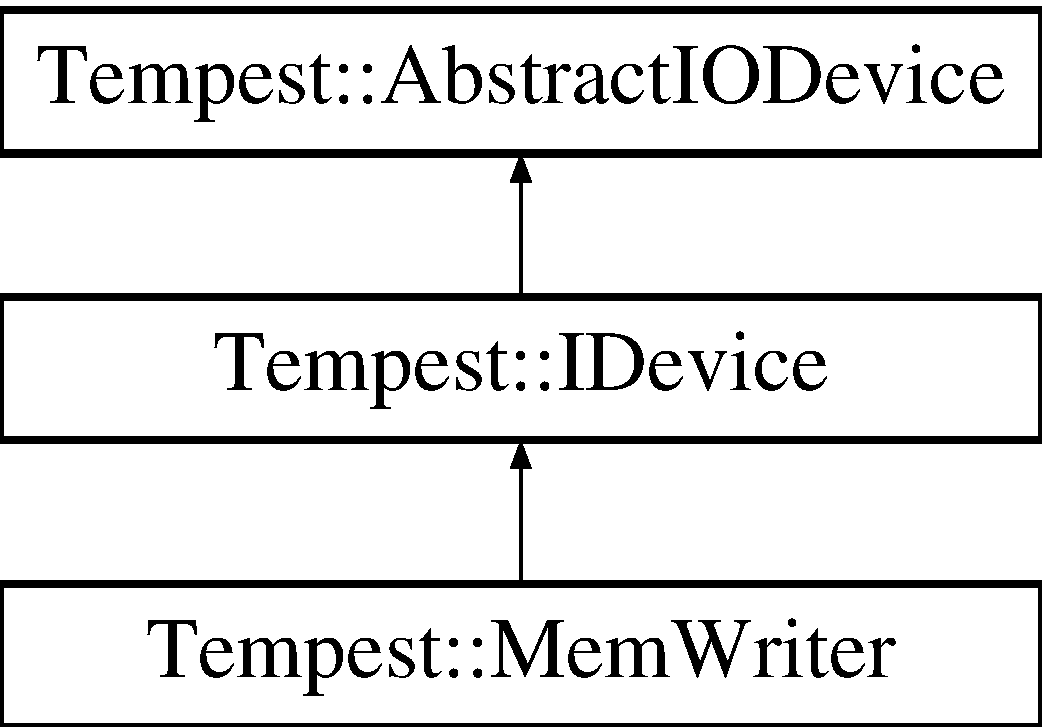
\includegraphics[height=3.000000cm]{class_tempest_1_1_mem_writer}
\end{center}
\end{figure}
\subsection*{Public Member Functions}
\begin{DoxyCompactItemize}
\item 
\hypertarget{class_tempest_1_1_mem_writer_aa20c388342a7939837fa5ee1b53db764}{{\bfseries Mem\+Writer} (char $\ast$vec, size\+\_\+t sz)}\label{class_tempest_1_1_mem_writer_aa20c388342a7939837fa5ee1b53db764}

\item 
\hypertarget{class_tempest_1_1_mem_writer_a8b6b7221970053fca5b8d730d43d81e9}{{\bfseries Mem\+Writer} (unsigned char $\ast$vec, size\+\_\+t sz)}\label{class_tempest_1_1_mem_writer_a8b6b7221970053fca5b8d730d43d81e9}

\item 
\hypertarget{class_tempest_1_1_mem_writer_afd6f03c7d6bc95ffe4c82f49ab82a29e}{size\+\_\+t {\bfseries write\+Data} (char $\ast$src, size\+\_\+t count)}\label{class_tempest_1_1_mem_writer_afd6f03c7d6bc95ffe4c82f49ab82a29e}

\end{DoxyCompactItemize}


The documentation for this class was generated from the following files\+:\begin{DoxyCompactItemize}
\item 
io/iodevice.\+h\item 
io/iodevice.\+cpp\end{DoxyCompactItemize}

\hypertarget{struct_direct_x9_1_1_i_b_o_1_1_min}{\section{Tempest\+:\+:Direct\+X9\+:\+:I\+B\+O\+:\+:Min Struct Reference}
\label{struct_direct_x9_1_1_i_b_o_1_1_min}\index{Tempest\+::\+Direct\+X9\+::\+I\+B\+O\+::\+Min@{Tempest\+::\+Direct\+X9\+::\+I\+B\+O\+::\+Min}}
}
\subsection*{Public Attributes}
\begin{DoxyCompactItemize}
\item 
\hypertarget{struct_direct_x9_1_1_i_b_o_1_1_min_a452904e56fa12fbc652b459daa45ecb6}{uint16\+\_\+t {\bfseries val}}\label{struct_direct_x9_1_1_i_b_o_1_1_min_a452904e56fa12fbc652b459daa45ecb6}

\item 
\hypertarget{struct_direct_x9_1_1_i_b_o_1_1_min_a6bff736ca595b8fb6429fc80c5d3fa30}{uint16\+\_\+t {\bfseries begin}}\label{struct_direct_x9_1_1_i_b_o_1_1_min_a6bff736ca595b8fb6429fc80c5d3fa30}

\item 
\hypertarget{struct_direct_x9_1_1_i_b_o_1_1_min_aedee791c893c09300d394f32e7b286d8}{uint16\+\_\+t {\bfseries size}}\label{struct_direct_x9_1_1_i_b_o_1_1_min_aedee791c893c09300d394f32e7b286d8}

\end{DoxyCompactItemize}


The documentation for this struct was generated from the following file\+:\begin{DoxyCompactItemize}
\item 
dx/directx9.\+cpp\end{DoxyCompactItemize}

\hypertarget{class_tempest_1_1_model}{\section{Tempest\+:\+:Model$<$ V $>$ Class Template Reference}
\label{class_tempest_1_1_model}\index{Tempest\+::\+Model$<$ V $>$@{Tempest\+::\+Model$<$ V $>$}}
}
\subsection*{Public Types}
\begin{DoxyCompactItemize}
\item 
\hypertarget{class_tempest_1_1_model_a62e8ff84f406936f893cf21f015bc1cc}{typedef Model\+Vertex {\bfseries Vertex}}\label{class_tempest_1_1_model_a62e8ff84f406936f893cf21f015bc1cc}

\item 
\hypertarget{class_tempest_1_1_model_a07e3ed85ca32136b470a1409f937798a}{typedef \hyperlink{struct_tempest_1_1_raw_model}{Raw\+Model}$<$ Vertex $>$ {\bfseries Raw}}\label{class_tempest_1_1_model_a07e3ed85ca32136b470a1409f937798a}

\end{DoxyCompactItemize}
\subsection*{Public Member Functions}
\begin{DoxyCompactItemize}
\item 
\hypertarget{class_tempest_1_1_model_a458bbce3012425791096999a08110620}{void {\bfseries load} (\hyperlink{class_tempest_1_1_vertex_buffer_holder}{Tempest\+::\+Vertex\+Buffer\+Holder} \&vbo\+Holder, \hyperlink{class_tempest_1_1_index_buffer_holder}{Tempest\+::\+Index\+Buffer\+Holder} \&, const Vertex $\ast$buf, size\+\_\+t buf\+Size, const \hyperlink{class_tempest_1_1_vertex_declaration_1_1_declarator}{Tempest\+::\+Vertex\+Declaration\+::\+Declarator} \&decl, Abstract\+A\+P\+I\+::\+Buffer\+Flag buffer\+Flag=Abstract\+A\+P\+I\+::\+B\+F\+\_\+\+No\+Flags)}\label{class_tempest_1_1_model_a458bbce3012425791096999a08110620}

\item 
\hypertarget{class_tempest_1_1_model_ab50eff71acf87f2066f88b54cdc58980}{void {\bfseries load} (\hyperlink{class_tempest_1_1_vertex_buffer_holder}{Tempest\+::\+Vertex\+Buffer\+Holder} \&vbo\+Holder, \hyperlink{class_tempest_1_1_index_buffer_holder}{Tempest\+::\+Index\+Buffer\+Holder} \&ibo\+Holder, const std\+::vector$<$ Vertex $>$ \&buf, const \hyperlink{class_tempest_1_1_vertex_declaration_1_1_declarator}{Tempest\+::\+Vertex\+Declaration\+::\+Declarator} \&decl, Abstract\+A\+P\+I\+::\+Buffer\+Flag buffer\+Flag=Abstract\+A\+P\+I\+::\+B\+F\+\_\+\+No\+Flags)}\label{class_tempest_1_1_model_ab50eff71acf87f2066f88b54cdc58980}

\item 
\hypertarget{class_tempest_1_1_model_acbfce05d4cd570aac5f43cc751630326}{void {\bfseries load} (\hyperlink{class_tempest_1_1_vertex_buffer_holder}{Tempest\+::\+Vertex\+Buffer\+Holder} \&vbo\+Holder, \hyperlink{class_tempest_1_1_index_buffer_holder}{Tempest\+::\+Index\+Buffer\+Holder} \&ibo\+Holder, const Vertex $\ast$buf, size\+\_\+t buf\+Size, const uint16\+\_\+t $\ast$index, size\+\_\+t ibo\+Size, const \hyperlink{class_tempest_1_1_vertex_declaration_1_1_declarator}{Tempest\+::\+Vertex\+Declaration\+::\+Declarator} \&decl, Abstract\+A\+P\+I\+::\+Buffer\+Flag buffer\+Flag=Abstract\+A\+P\+I\+::\+B\+F\+\_\+\+No\+Flags)}\label{class_tempest_1_1_model_acbfce05d4cd570aac5f43cc751630326}

\item 
\hypertarget{class_tempest_1_1_model_af3fd35531e7d151de2bcb5db961b79ca}{void {\bfseries load} (\hyperlink{class_tempest_1_1_vertex_buffer_holder}{Tempest\+::\+Vertex\+Buffer\+Holder} \&vbo\+Holder, \hyperlink{class_tempest_1_1_index_buffer_holder}{Tempest\+::\+Index\+Buffer\+Holder} \&ibo\+Holder, const std\+::vector$<$ Vertex $>$ \&buf, const std\+::vector$<$ uint16\+\_\+t $>$ \&index, const \hyperlink{class_tempest_1_1_vertex_declaration_1_1_declarator}{Tempest\+::\+Vertex\+Declaration\+::\+Declarator} \&decl, Abstract\+A\+P\+I\+::\+Buffer\+Flag buffer\+Flag=Abstract\+A\+P\+I\+::\+B\+F\+\_\+\+No\+Flags)}\label{class_tempest_1_1_model_af3fd35531e7d151de2bcb5db961b79ca}

\item 
\hypertarget{class_tempest_1_1_model_a04e8562a09de8cb7094bf41161ab575d}{void {\bfseries load} (\hyperlink{class_tempest_1_1_vertex_buffer_holder}{Tempest\+::\+Vertex\+Buffer\+Holder} \&vbo\+Holder, \hyperlink{class_tempest_1_1_index_buffer_holder}{Tempest\+::\+Index\+Buffer\+Holder} \&ibo\+Holder, const \hyperlink{struct_tempest_1_1_raw_model}{Raw} \&data, const \hyperlink{class_tempest_1_1_vertex_declaration_1_1_declarator}{Tempest\+::\+Vertex\+Declaration\+::\+Declarator} \&decl, Abstract\+A\+P\+I\+::\+Buffer\+Flag buffer\+Flag=Abstract\+A\+P\+I\+::\+B\+F\+\_\+\+No\+Flags)}\label{class_tempest_1_1_model_a04e8562a09de8cb7094bf41161ab575d}

\item 
\hypertarget{class_tempest_1_1_model_adcff6e557a566dcd92ffa4ca2a7de9d1}{void {\bfseries load} (\hyperlink{class_tempest_1_1_vertex_buffer_holder}{Tempest\+::\+Vertex\+Buffer\+Holder} \&vbo\+Holder, \hyperlink{class_tempest_1_1_index_buffer_holder}{Tempest\+::\+Index\+Buffer\+Holder} \&ibo\+Holder, const std\+::string \&fname)}\label{class_tempest_1_1_model_adcff6e557a566dcd92ffa4ca2a7de9d1}

\item 
\hypertarget{class_tempest_1_1_model_a98d8268bde1100749871000e87995f44}{void {\bfseries load} (const \hyperlink{class_tempest_1_1_vertex_buffer}{Tempest\+::\+Vertex\+Buffer}$<$ Vertex $>$ \&v, const \hyperlink{class_tempest_1_1_index_buffer}{Tempest\+::\+Index\+Buffer}$<$ uint16\+\_\+t $>$ \&i, const \hyperlink{class_tempest_1_1_vertex_declaration}{Tempest\+::\+Vertex\+Declaration} \&d)}\label{class_tempest_1_1_model_a98d8268bde1100749871000e87995f44}

\item 
\hypertarget{class_tempest_1_1_model_a539f38d517daa18f885210e0f8c1f56c}{void {\bfseries load} (const \hyperlink{class_tempest_1_1_vertex_buffer}{Tempest\+::\+Vertex\+Buffer}$<$ Model\+Vertex $>$ \&v, const \hyperlink{class_tempest_1_1_vertex_declaration}{Tempest\+::\+Vertex\+Declaration} \&d)}\label{class_tempest_1_1_model_a539f38d517daa18f885210e0f8c1f56c}

\item 
\hypertarget{class_tempest_1_1_model_a0f02d911bc4a510abc613ec6c74fcbc3}{const \hyperlink{class_tempest_1_1_vertex_buffer}{Vertex\+Buffer}$<$ Vertex $>$ \& {\bfseries vertexes} () const }\label{class_tempest_1_1_model_a0f02d911bc4a510abc613ec6c74fcbc3}

\item 
\hypertarget{class_tempest_1_1_model_afbb56bbf5eb1c3d3d25caa7901e7973b}{const \hyperlink{class_tempest_1_1_index_buffer}{Index\+Buffer}$<$ uint16\+\_\+t $>$ \& {\bfseries indexes} () const }\label{class_tempest_1_1_model_afbb56bbf5eb1c3d3d25caa7901e7973b}

\item 
\hypertarget{class_tempest_1_1_model_a2980dc670aed2e64cb1493c95b2958e6}{const \hyperlink{class_tempest_1_1_vertex_declaration}{Tempest\+::\+Vertex\+Declaration} \& {\bfseries declaration} () const }\label{class_tempest_1_1_model_a2980dc670aed2e64cb1493c95b2958e6}

\item 
\hypertarget{class_tempest_1_1_model_a139aadbec813ec242926cfd0cd767768}{int {\bfseries size} () const }\label{class_tempest_1_1_model_a139aadbec813ec242926cfd0cd767768}

\item 
\hypertarget{class_tempest_1_1_model_a9f605fc6893bf1dc1732267708d49062}{int {\bfseries vertex\+Count} () const }\label{class_tempest_1_1_model_a9f605fc6893bf1dc1732267708d49062}

\item 
\hypertarget{class_tempest_1_1_model_afc0b71b9ccaddf52f10b50ee5a1a28ce}{const \hyperlink{struct_tempest_1_1_model_bounds}{Model\+Bounds} \& {\bfseries bounds} () const }\label{class_tempest_1_1_model_afc0b71b9ccaddf52f10b50ee5a1a28ce}

\item 
\hypertarget{class_tempest_1_1_model_a3cb339eeb2172693b62b97f18aadfd56}{Tempest\+::\+Abstract\+A\+P\+I\+::\+Primitive\+Type {\bfseries primitive\+Type} () const }\label{class_tempest_1_1_model_a3cb339eeb2172693b62b97f18aadfd56}

\item 
\hypertarget{class_tempest_1_1_model_a696b7ee7bbb3a8d3ca948234608f1eb7}{size\+\_\+t {\bfseries primitive\+Count} () const }\label{class_tempest_1_1_model_a696b7ee7bbb3a8d3ca948234608f1eb7}

\item 
\hypertarget{class_tempest_1_1_model_a2f38ca7e86fb29d1f1369f6b747e26e4}{\hyperlink{class_tempest_1_1_model}{Model}$<$ Model\+Vertex $>$ {\bfseries slice} (int first, int size) const }\label{class_tempest_1_1_model_a2f38ca7e86fb29d1f1369f6b747e26e4}

\item 
\hypertarget{class_tempest_1_1_model_a6c870dd7ec9cf0a7450a84b049c397ca}{\hyperlink{class_tempest_1_1_model}{Model}$<$ Model\+Vertex $>$ {\bfseries slice} (int first) const }\label{class_tempest_1_1_model_a6c870dd7ec9cf0a7450a84b049c397ca}

\end{DoxyCompactItemize}
\subsection*{Static Public Member Functions}
\begin{DoxyCompactItemize}
\item 
\hypertarget{class_tempest_1_1_model_a5ce67e48f77f722ea7ca8d6ed4c0af4e}{static \hyperlink{struct_tempest_1_1_raw_model}{Raw} {\bfseries load\+Raw\+Data} (const std\+::string \&fname)}\label{class_tempest_1_1_model_a5ce67e48f77f722ea7ca8d6ed4c0af4e}

\item 
\hypertarget{class_tempest_1_1_model_a959c4a4665a6c2d3ad21e858a87717bc}{static bool {\bfseries save\+Raw\+Data} (const std\+::string \&fname, const \hyperlink{struct_tempest_1_1_raw_model}{Raw} \&r)}\label{class_tempest_1_1_model_a959c4a4665a6c2d3ad21e858a87717bc}

\end{DoxyCompactItemize}


The documentation for this class was generated from the following files\+:\begin{DoxyCompactItemize}
\item 
scene/abstractgraphicobject.\+h\item 
scene/model.\+h\end{DoxyCompactItemize}

\hypertarget{struct_tempest_1_1_model_bounds}{\section{Tempest\+:\+:Model\+Bounds Struct Reference}
\label{struct_tempest_1_1_model_bounds}\index{Tempest\+::\+Model\+Bounds@{Tempest\+::\+Model\+Bounds}}
}
\subsection*{Public Member Functions}
\begin{DoxyCompactItemize}
\item 
\hypertarget{struct_tempest_1_1_model_bounds_af56a2ca25e923d0986ba3d6d80177b42}{float {\bfseries diameter} () const }\label{struct_tempest_1_1_model_bounds_af56a2ca25e923d0986ba3d6d80177b42}

\item 
\hypertarget{struct_tempest_1_1_model_bounds_a0a1570f914547d59035ffa7538a643d5}{float {\bfseries radius} () const }\label{struct_tempest_1_1_model_bounds_a0a1570f914547d59035ffa7538a643d5}

\end{DoxyCompactItemize}
\subsection*{Public Attributes}
\begin{DoxyCompactItemize}
\item 
\hypertarget{struct_tempest_1_1_model_bounds_afcd0da5fe0be8195f184db02ec351500}{float {\bfseries min} \mbox{[}3\mbox{]}}\label{struct_tempest_1_1_model_bounds_afcd0da5fe0be8195f184db02ec351500}

\item 
\hypertarget{struct_tempest_1_1_model_bounds_a870dc0c987a754fd7fc71655eefc260d}{float {\bfseries max} \mbox{[}3\mbox{]}}\label{struct_tempest_1_1_model_bounds_a870dc0c987a754fd7fc71655eefc260d}

\item 
\hypertarget{struct_tempest_1_1_model_bounds_a88cc5797a42f0c8430cb25d1551f90aa}{float {\bfseries mid} \mbox{[}3\mbox{]}}\label{struct_tempest_1_1_model_bounds_a88cc5797a42f0c8430cb25d1551f90aa}

\end{DoxyCompactItemize}


The documentation for this struct was generated from the following files\+:\begin{DoxyCompactItemize}
\item 
scene/model.\+h\item 
scene/model.\+cpp\end{DoxyCompactItemize}

\hypertarget{class_tempest_1_1_mouse_event}{\section{Tempest\+:\+:Mouse\+Event Class Reference}
\label{class_tempest_1_1_mouse_event}\index{Tempest\+::\+Mouse\+Event@{Tempest\+::\+Mouse\+Event}}
}
Inheritance diagram for Tempest\+:\+:Mouse\+Event\+:\begin{figure}[H]
\begin{center}
\leavevmode
\includegraphics[height=2.000000cm]{class_tempest_1_1_mouse_event}
\end{center}
\end{figure}
\subsection*{Public Member Functions}
\begin{DoxyCompactItemize}
\item 
\hypertarget{class_tempest_1_1_mouse_event_a61783f8a11fd73170bda9a2b2cf3665f}{{\bfseries Mouse\+Event} (int mx=-\/1, int my=-\/1, Mouse\+Button b=Button\+None, int mdelta=0, int mouse\+I\+D=0, Type t=Mouse\+Move)}\label{class_tempest_1_1_mouse_event_a61783f8a11fd73170bda9a2b2cf3665f}

\item 
\hypertarget{class_tempest_1_1_mouse_event_a3a4b8f92923d95beb904bcdb4f15276d}{\hyperlink{struct_tempest_1_1_point}{Point} {\bfseries pos} () const }\label{class_tempest_1_1_mouse_event_a3a4b8f92923d95beb904bcdb4f15276d}

\end{DoxyCompactItemize}
\subsection*{Public Attributes}
\begin{DoxyCompactItemize}
\item 
\hypertarget{class_tempest_1_1_mouse_event_a8e1c63ccedd5bb6213891de0a441e6f4}{const int {\bfseries x}}\label{class_tempest_1_1_mouse_event_a8e1c63ccedd5bb6213891de0a441e6f4}

\item 
\hypertarget{class_tempest_1_1_mouse_event_ae8e7232e1c7af737513f2712cd860cea}{const int {\bfseries y}}\label{class_tempest_1_1_mouse_event_ae8e7232e1c7af737513f2712cd860cea}

\item 
\hypertarget{class_tempest_1_1_mouse_event_af59e72cfe86c61bc41143f4035607c52}{const int {\bfseries delta}}\label{class_tempest_1_1_mouse_event_af59e72cfe86c61bc41143f4035607c52}

\item 
\hypertarget{class_tempest_1_1_mouse_event_ac5a87cdb74aafc1fd472ee77b776973a}{const Mouse\+Button {\bfseries button}}\label{class_tempest_1_1_mouse_event_ac5a87cdb74aafc1fd472ee77b776973a}

\item 
\hypertarget{class_tempest_1_1_mouse_event_a1922afc293095cba9f7b56ce69d7e3d0}{const int {\bfseries mouse\+I\+D}}\label{class_tempest_1_1_mouse_event_a1922afc293095cba9f7b56ce69d7e3d0}

\end{DoxyCompactItemize}
\subsection*{Additional Inherited Members}


\subsection{Detailed Description}
\begin{Desc}
\item[Examples\+: ]\par
\hyperlink{_cube_2mainwindow_8cpp-example}{Cube/mainwindow.\+cpp}, \hyperlink{_cube_2mainwindow_8h-example}{Cube/mainwindow.\+h}, \hyperlink{_painting2d_2mainwindow_8cpp-example}{Painting2d/mainwindow.\+cpp}, and \hyperlink{_painting2d_2mainwindow_8h-example}{Painting2d/mainwindow.\+h}.\end{Desc}


The documentation for this class was generated from the following files\+:\begin{DoxyCompactItemize}
\item 
ui/event.\+h\item 
ui/event.\+cpp\end{DoxyCompactItemize}

\hypertarget{struct_tempest_1_1_local_textures_holder_1_1_non_freed}{\section{Tempest\+:\+:Local\+Textures\+Holder\+:\+:Non\+Freed Struct Reference}
\label{struct_tempest_1_1_local_textures_holder_1_1_non_freed}\index{Tempest\+::\+Local\+Textures\+Holder\+::\+Non\+Freed@{Tempest\+::\+Local\+Textures\+Holder\+::\+Non\+Freed}}
}
\subsection*{Public Attributes}
\begin{DoxyCompactItemize}
\item 
\hypertarget{struct_tempest_1_1_local_textures_holder_1_1_non_freed_a27ac0857b03fd788263f912fafbfebe3}{\hyperlink{struct_tempest_1_1_local_textures_holder_1_1_non_freed_data}{Non\+Freed\+Data} {\bfseries data}}\label{struct_tempest_1_1_local_textures_holder_1_1_non_freed_a27ac0857b03fd788263f912fafbfebe3}

\item 
\hypertarget{struct_tempest_1_1_local_textures_holder_1_1_non_freed_ac4ff2bd68300b1798d94561319b39b8f}{int {\bfseries collect\+Iteration}}\label{struct_tempest_1_1_local_textures_holder_1_1_non_freed_ac4ff2bd68300b1798d94561319b39b8f}

\item 
\hypertarget{struct_tempest_1_1_local_textures_holder_1_1_non_freed_acbb90184c467fc441c6f25886d0fa859}{void $\ast$ {\bfseries user\+Ptr}}\label{struct_tempest_1_1_local_textures_holder_1_1_non_freed_acbb90184c467fc441c6f25886d0fa859}

\end{DoxyCompactItemize}


The documentation for this struct was generated from the following file\+:\begin{DoxyCompactItemize}
\item 
data\+Control/localtexturesholder.\+h\end{DoxyCompactItemize}

\hypertarget{struct_tempest_1_1_local_buffer_holder_1_1_non_freed}{\section{Tempest\+:\+:Local\+Buffer\+Holder$<$ Holder $>$\+:\+:Non\+Freed Struct Reference}
\label{struct_tempest_1_1_local_buffer_holder_1_1_non_freed}\index{Tempest\+::\+Local\+Buffer\+Holder$<$ Holder $>$\+::\+Non\+Freed@{Tempest\+::\+Local\+Buffer\+Holder$<$ Holder $>$\+::\+Non\+Freed}}
}
\subsection*{Public Attributes}
\begin{DoxyCompactItemize}
\item 
\hypertarget{struct_tempest_1_1_local_buffer_holder_1_1_non_freed_a19f0314c767b5bbb0e24cd2e3c8e6b2b}{\hyperlink{struct_tempest_1_1_local_buffer_holder_1_1_non_freed_data}{Non\+Freed\+Data} {\bfseries data}}\label{struct_tempest_1_1_local_buffer_holder_1_1_non_freed_a19f0314c767b5bbb0e24cd2e3c8e6b2b}

\item 
\hypertarget{struct_tempest_1_1_local_buffer_holder_1_1_non_freed_ab1fc2dcda0f60d1ec1e3cf12137faf0c}{int {\bfseries collect\+Iteration}}\label{struct_tempest_1_1_local_buffer_holder_1_1_non_freed_ab1fc2dcda0f60d1ec1e3cf12137faf0c}

\item 
\hypertarget{struct_tempest_1_1_local_buffer_holder_1_1_non_freed_a1f81bf6a9b1e189b681529b110f859c4}{void $\ast$ {\bfseries user\+Ptr}}\label{struct_tempest_1_1_local_buffer_holder_1_1_non_freed_a1f81bf6a9b1e189b681529b110f859c4}

\end{DoxyCompactItemize}


The documentation for this struct was generated from the following file\+:\begin{DoxyCompactItemize}
\item 
data\+Control/localvertexbufferholder.\+h\end{DoxyCompactItemize}

\hypertarget{struct_tempest_1_1_local_textures_holder_1_1_non_freed_data}{\section{Tempest\+:\+:Local\+Textures\+Holder\+:\+:Non\+Freed\+Data Struct Reference}
\label{struct_tempest_1_1_local_textures_holder_1_1_non_freed_data}\index{Tempest\+::\+Local\+Textures\+Holder\+::\+Non\+Freed\+Data@{Tempest\+::\+Local\+Textures\+Holder\+::\+Non\+Freed\+Data}}
}
\subsection*{Public Member Functions}
\begin{DoxyCompactItemize}
\item 
\hypertarget{struct_tempest_1_1_local_textures_holder_1_1_non_freed_data_a8fe349c8ea7b769d23e7a60a631ad5d2}{bool {\bfseries operator==} (const \hyperlink{struct_tempest_1_1_local_textures_holder_1_1_non_freed_data}{Non\+Freed\+Data} \&b) const }\label{struct_tempest_1_1_local_textures_holder_1_1_non_freed_data_a8fe349c8ea7b769d23e7a60a631ad5d2}

\end{DoxyCompactItemize}
\subsection*{Public Attributes}
\begin{DoxyCompactItemize}
\item 
\hypertarget{struct_tempest_1_1_local_textures_holder_1_1_non_freed_data_abb665ee3625f1ba54b2d2075d622cc75}{Tempest\+::\+Abstract\+A\+P\+I\+::\+Texture $\ast$ {\bfseries handle}}\label{struct_tempest_1_1_local_textures_holder_1_1_non_freed_data_abb665ee3625f1ba54b2d2075d622cc75}

\item 
\hypertarget{struct_tempest_1_1_local_textures_holder_1_1_non_freed_data_ac710cc9d0d5edc1d17706b05a5e7e17f}{int {\bfseries w}}\label{struct_tempest_1_1_local_textures_holder_1_1_non_freed_data_ac710cc9d0d5edc1d17706b05a5e7e17f}

\item 
\hypertarget{struct_tempest_1_1_local_textures_holder_1_1_non_freed_data_adae8df1fa7dcee1dea07953be9150933}{int {\bfseries h}}\label{struct_tempest_1_1_local_textures_holder_1_1_non_freed_data_adae8df1fa7dcee1dea07953be9150933}

\item 
\hypertarget{struct_tempest_1_1_local_textures_holder_1_1_non_freed_data_a893bc20620010ab42d9c16cab0e0c570}{bool {\bfseries mip}}\label{struct_tempest_1_1_local_textures_holder_1_1_non_freed_data_a893bc20620010ab42d9c16cab0e0c570}

\item 
\hypertarget{struct_tempest_1_1_local_textures_holder_1_1_non_freed_data_a2d146d1bfde53b0cce3f8acced55c57b}{bool {\bfseries compress}}\label{struct_tempest_1_1_local_textures_holder_1_1_non_freed_data_a2d146d1bfde53b0cce3f8acced55c57b}

\item 
\hypertarget{struct_tempest_1_1_local_textures_holder_1_1_non_freed_data_a3bf2ec89f266c8c3c710c57356c583cf}{\hyperlink{struct_tempest_1_1_abstract_texture_1_1_format_a231a1f516e53783bf72c713669b115b3}{Tempest\+::\+Abstract\+Texture\+::\+Format\+::\+Type} {\bfseries format}}\label{struct_tempest_1_1_local_textures_holder_1_1_non_freed_data_a3bf2ec89f266c8c3c710c57356c583cf}

\item 
\hypertarget{struct_tempest_1_1_local_textures_holder_1_1_non_freed_data_a9b388e43c74af372144ae3a670432534}{Tempest\+::\+Texture\+Usage {\bfseries usage}}\label{struct_tempest_1_1_local_textures_holder_1_1_non_freed_data_a9b388e43c74af372144ae3a670432534}

\item 
\hypertarget{struct_tempest_1_1_local_textures_holder_1_1_non_freed_data_a3ab2f99a853b750cf3bb406d0e37fac3}{bool {\bfseries dynamic}}\label{struct_tempest_1_1_local_textures_holder_1_1_non_freed_data_a3ab2f99a853b750cf3bb406d0e37fac3}

\item 
\hypertarget{struct_tempest_1_1_local_textures_holder_1_1_non_freed_data_a21da4bc9fb54f4853196b4acc476ba47}{bool {\bfseries restore\+Intent}}\label{struct_tempest_1_1_local_textures_holder_1_1_non_freed_data_a21da4bc9fb54f4853196b4acc476ba47}

\end{DoxyCompactItemize}


The documentation for this struct was generated from the following file\+:\begin{DoxyCompactItemize}
\item 
data\+Control/localtexturesholder.\+h\end{DoxyCompactItemize}

\hypertarget{struct_tempest_1_1_local_buffer_holder_1_1_non_freed_data}{\section{Tempest\+:\+:Local\+Buffer\+Holder$<$ Holder $>$\+:\+:Non\+Freed\+Data Struct Reference}
\label{struct_tempest_1_1_local_buffer_holder_1_1_non_freed_data}\index{Tempest\+::\+Local\+Buffer\+Holder$<$ Holder $>$\+::\+Non\+Freed\+Data@{Tempest\+::\+Local\+Buffer\+Holder$<$ Holder $>$\+::\+Non\+Freed\+Data}}
}
\subsection*{Public Attributes}
\begin{DoxyCompactItemize}
\item 
\hypertarget{struct_tempest_1_1_local_buffer_holder_1_1_non_freed_data_a2bca51017688a8138fcf1fd018304cbf}{Holder\+::\+Descriptor\+Type $\ast$ {\bfseries handle}}\label{struct_tempest_1_1_local_buffer_holder_1_1_non_freed_data_a2bca51017688a8138fcf1fd018304cbf}

\item 
\hypertarget{struct_tempest_1_1_local_buffer_holder_1_1_non_freed_data_a225a995fda4f6b25c9587badd0091394}{int {\bfseries mem\+Size}}\label{struct_tempest_1_1_local_buffer_holder_1_1_non_freed_data_a225a995fda4f6b25c9587badd0091394}

\item 
\hypertarget{struct_tempest_1_1_local_buffer_holder_1_1_non_freed_data_aa738b06aa07f1ac9376b798a320a8af9}{int {\bfseries el\+Size}}\label{struct_tempest_1_1_local_buffer_holder_1_1_non_freed_data_aa738b06aa07f1ac9376b798a320a8af9}

\item 
\hypertarget{struct_tempest_1_1_local_buffer_holder_1_1_non_freed_data_abf136df1921b63bdbb6991ecd078b43e}{bool {\bfseries restore\+Intent}}\label{struct_tempest_1_1_local_buffer_holder_1_1_non_freed_data_abf136df1921b63bdbb6991ecd078b43e}

\end{DoxyCompactItemize}


The documentation for this struct was generated from the following file\+:\begin{DoxyCompactItemize}
\item 
data\+Control/localvertexbufferholder.\+h\end{DoxyCompactItemize}

\hypertarget{class_tempest_1_1_o_device}{\section{Tempest\+:\+:O\+Device Class Reference}
\label{class_tempest_1_1_o_device}\index{Tempest\+::\+O\+Device@{Tempest\+::\+O\+Device}}
}
Inheritance diagram for Tempest\+:\+:O\+Device\+:\begin{figure}[H]
\begin{center}
\leavevmode
\includegraphics[height=3.000000cm]{class_tempest_1_1_o_device}
\end{center}
\end{figure}
\subsection*{Public Member Functions}
\begin{DoxyCompactItemize}
\item 
\hypertarget{class_tempest_1_1_o_device_a6f6971a9028adaf99df03843384de797}{virtual size\+\_\+t {\bfseries write\+Data} (const char $\ast$src, size\+\_\+t count)=0}\label{class_tempest_1_1_o_device_a6f6971a9028adaf99df03843384de797}

\item 
\hypertarget{class_tempest_1_1_o_device_aee7a02b15a9173101bdcbdda6d08296a}{virtual void {\bfseries flush} ()}\label{class_tempest_1_1_o_device_aee7a02b15a9173101bdcbdda6d08296a}

\end{DoxyCompactItemize}


The documentation for this class was generated from the following files\+:\begin{DoxyCompactItemize}
\item 
io/iodevice.\+h\item 
io/iodevice.\+cpp\end{DoxyCompactItemize}

\hypertarget{class_tempest_1_1_opengl2x}{\section{Tempest\+:\+:Opengl2x Class Reference}
\label{class_tempest_1_1_opengl2x}\index{Tempest\+::\+Opengl2x@{Tempest\+::\+Opengl2x}}
}
Inheritance diagram for Tempest\+:\+:Opengl2x\+:\begin{figure}[H]
\begin{center}
\leavevmode
\includegraphics[height=3.000000cm]{class_tempest_1_1_opengl2x}
\end{center}
\end{figure}
\subsection*{Classes}
\begin{DoxyCompactItemize}
\item 
struct \hyperlink{struct_tempest_1_1_opengl2x_1_1_device}{Device}
\end{DoxyCompactItemize}
\subsection*{Public Member Functions}
\begin{DoxyCompactItemize}
\item 
\hypertarget{class_tempest_1_1_opengl2x_a3607dc06ac4a37093cce804a8000f947}{\hyperlink{struct_tempest_1_1_abstract_a_p_i_1_1_caps}{Caps} {\bfseries caps} (\hyperlink{struct_tempest_1_1_opengl2x_1_1_device}{Device} $\ast$d) const }\label{class_tempest_1_1_opengl2x_a3607dc06ac4a37093cce804a8000f947}

\item 
\hypertarget{class_tempest_1_1_opengl2x_a8cd7d319b424b6c9c33d18e4a122983e}{std\+::string {\bfseries vendor} (Abstract\+A\+P\+I\+::\+Device $\ast$d) const }\label{class_tempest_1_1_opengl2x_a8cd7d319b424b6c9c33d18e4a122983e}

\item 
\hypertarget{class_tempest_1_1_opengl2x_a284cc8666959b8799de5c277de4fffb6}{std\+::string {\bfseries renderer} (Abstract\+A\+P\+I\+::\+Device $\ast$d) const }\label{class_tempest_1_1_opengl2x_a284cc8666959b8799de5c277de4fffb6}

\item 
\hypertarget{class_tempest_1_1_opengl2x_a9b19542a96f89364feb5b6f80cecc7e0}{\hyperlink{struct_tempest_1_1_opengl2x_1_1_device}{Device} $\ast$ {\bfseries create\+Device} (void $\ast$hwnd, const \hyperlink{struct_tempest_1_1_abstract_a_p_i_1_1_options}{Options} \&opt) const }\label{class_tempest_1_1_opengl2x_a9b19542a96f89364feb5b6f80cecc7e0}

\item 
\hypertarget{class_tempest_1_1_opengl2x_ac5af4fe226794b139a7304dff6dc7dc2}{void {\bfseries delete\+Device} (\hyperlink{struct_tempest_1_1_opengl2x_1_1_device}{Device} $\ast$d) const }\label{class_tempest_1_1_opengl2x_ac5af4fe226794b139a7304dff6dc7dc2}

\item 
\hypertarget{class_tempest_1_1_opengl2x_ab2b0cb4294e11eeb642371e8ef56c0da}{void {\bfseries clear} (Abstract\+A\+P\+I\+::\+Device $\ast$d, const \hyperlink{class_tempest_1_1_color}{Color} \&cl, float z, unsigned stencil) const }\label{class_tempest_1_1_opengl2x_ab2b0cb4294e11eeb642371e8ef56c0da}

\item 
\hypertarget{class_tempest_1_1_opengl2x_a322eed312d9870f75e73bcd0d953d526}{void {\bfseries clear} (Abstract\+A\+P\+I\+::\+Device $\ast$d, const \hyperlink{class_tempest_1_1_color}{Color} \&cl) const }\label{class_tempest_1_1_opengl2x_a322eed312d9870f75e73bcd0d953d526}

\item 
\hypertarget{class_tempest_1_1_opengl2x_ac420d72c9589796b2d64edb14475b3a1}{void {\bfseries clear} (Abstract\+A\+P\+I\+::\+Device $\ast$d, const \hyperlink{class_tempest_1_1_color}{Color} \&cl, float z) const }\label{class_tempest_1_1_opengl2x_ac420d72c9589796b2d64edb14475b3a1}

\item 
\hypertarget{class_tempest_1_1_opengl2x_a66fdc55ebe93631248c801905db423d1}{void {\bfseries clear} (Abstract\+A\+P\+I\+::\+Device $\ast$d, float z, unsigned stencil) const }\label{class_tempest_1_1_opengl2x_a66fdc55ebe93631248c801905db423d1}

\item 
\hypertarget{class_tempest_1_1_opengl2x_a50ead43b774de766d2388301e68b0884}{void {\bfseries clear\+Z} (Abstract\+A\+P\+I\+::\+Device $\ast$d, float z) const }\label{class_tempest_1_1_opengl2x_a50ead43b774de766d2388301e68b0884}

\item 
\hypertarget{class_tempest_1_1_opengl2x_a54854cb3d08884680ed3aaf4a7a0e7f3}{void {\bfseries clear\+Stencil} (Abstract\+A\+P\+I\+::\+Device $\ast$d, unsigned stencil) const }\label{class_tempest_1_1_opengl2x_a54854cb3d08884680ed3aaf4a7a0e7f3}

\item 
\hypertarget{class_tempest_1_1_opengl2x_a08fdaf1c11f42dc1200cb91505474510}{void {\bfseries begin\+Paint} (Abstract\+A\+P\+I\+::\+Device $\ast$d) const }\label{class_tempest_1_1_opengl2x_a08fdaf1c11f42dc1200cb91505474510}

\item 
\hypertarget{class_tempest_1_1_opengl2x_a0aa845a49200c9502c06e32be8a21a84}{void {\bfseries end\+Paint} (Abstract\+A\+P\+I\+::\+Device $\ast$d) const }\label{class_tempest_1_1_opengl2x_a0aa845a49200c9502c06e32be8a21a84}

\item 
\hypertarget{class_tempest_1_1_opengl2x_a595b512f8f332d8f043bf79438db66b6}{void {\bfseries set\+Render\+State} (\hyperlink{struct_tempest_1_1_opengl2x_1_1_device}{Device} $\ast$d, const \hyperlink{class_tempest_1_1_render_state}{Render\+State} \&) const }\label{class_tempest_1_1_opengl2x_a595b512f8f332d8f043bf79438db66b6}

\item 
\hypertarget{class_tempest_1_1_opengl2x_a76416f605848c6dbf9663fa7aa7965c5}{void {\bfseries set\+Render\+Taget} (Abstract\+A\+P\+I\+::\+Device $\ast$d, Abstract\+A\+P\+I\+::\+Texture $\ast$tx, int mip, int mrt\+Slot) const }\label{class_tempest_1_1_opengl2x_a76416f605848c6dbf9663fa7aa7965c5}

\item 
\hypertarget{class_tempest_1_1_opengl2x_a54460147baab85a097a8fe25b6893e40}{void {\bfseries unset\+Render\+Tagets} (Abstract\+A\+P\+I\+::\+Device $\ast$d, int count) const }\label{class_tempest_1_1_opengl2x_a54460147baab85a097a8fe25b6893e40}

\item 
\hypertarget{class_tempest_1_1_opengl2x_a00e95c6c75325d059090ad6fe554dc33}{void {\bfseries set\+D\+S\+Surface\+Taget} (Abstract\+A\+P\+I\+::\+Device $\ast$d, Std\+D\+S\+Surface $\ast$tx) const }\label{class_tempest_1_1_opengl2x_a00e95c6c75325d059090ad6fe554dc33}

\item 
\hypertarget{class_tempest_1_1_opengl2x_a194641f39ced16715135bebfd8cc09fc}{void {\bfseries set\+D\+S\+Surface\+Taget} (Abstract\+A\+P\+I\+::\+Device $\ast$d, Abstract\+A\+P\+I\+::\+Texture $\ast$tx) const }\label{class_tempest_1_1_opengl2x_a194641f39ced16715135bebfd8cc09fc}

\item 
\hypertarget{class_tempest_1_1_opengl2x_a6597bfa5444a239c91764644276c92d8}{Abstract\+A\+P\+I\+::\+Std\+D\+S\+Surface $\ast$ {\bfseries get\+D\+S\+Surface\+Taget} (Abstract\+A\+P\+I\+::\+Device $\ast$d) const }\label{class_tempest_1_1_opengl2x_a6597bfa5444a239c91764644276c92d8}

\item 
\hypertarget{class_tempest_1_1_opengl2x_a5f664d2fe2ef10a548a70b38846e6723}{void {\bfseries ret\+D\+S\+Surface\+Taget} (Abstract\+A\+P\+I\+::\+Device $\ast$d, Abstract\+A\+P\+I\+::\+Std\+D\+S\+Surface $\ast$s) const }\label{class_tempest_1_1_opengl2x_a5f664d2fe2ef10a548a70b38846e6723}

\item 
\hypertarget{class_tempest_1_1_opengl2x_a1b1eda3a8f736df9f281170b6c280738}{bool {\bfseries start\+Render} (Abstract\+A\+P\+I\+::\+Device $\ast$d, bool is\+Lost) const }\label{class_tempest_1_1_opengl2x_a1b1eda3a8f736df9f281170b6c280738}

\item 
\hypertarget{class_tempest_1_1_opengl2x_a3fcfdbd327882af5d6c744307ea0465d}{bool {\bfseries present} (Abstract\+A\+P\+I\+::\+Device $\ast$d, Swap\+Behavior b) const }\label{class_tempest_1_1_opengl2x_a3fcfdbd327882af5d6c744307ea0465d}

\item 
\hypertarget{class_tempest_1_1_opengl2x_aee904b7004535a3153413de4355408da}{bool {\bfseries reset} (Abstract\+A\+P\+I\+::\+Device $\ast$d, void $\ast$hwnd, const \hyperlink{struct_tempest_1_1_abstract_a_p_i_1_1_options}{Options} \&opt) const }\label{class_tempest_1_1_opengl2x_aee904b7004535a3153413de4355408da}

\item 
\hypertarget{class_tempest_1_1_opengl2x_a897c816674832bf85702dc6dc0c3e60b}{bool {\bfseries is\+Format\+Supported} (Abstract\+A\+P\+I\+::\+Device $\ast$d, Pixmap\+::\+Format f) const }\label{class_tempest_1_1_opengl2x_a897c816674832bf85702dc6dc0c3e60b}

\item 
\hypertarget{class_tempest_1_1_opengl2x_a119931c4eee3294455c4db27598b3d64}{Abstract\+A\+P\+I\+::\+Texture $\ast$ {\bfseries create\+Texture} (Abstract\+A\+P\+I\+::\+Device $\ast$d, const std\+::string \&) const }\label{class_tempest_1_1_opengl2x_a119931c4eee3294455c4db27598b3d64}

\item 
\hypertarget{class_tempest_1_1_opengl2x_a95e6a4d05d04a4733880e3b411a7755d}{Abstract\+A\+P\+I\+::\+Texture $\ast$ {\bfseries create\+Texture} (Abstract\+A\+P\+I\+::\+Device $\ast$d, const \hyperlink{class_tempest_1_1_pixmap}{Pixmap} \&p, bool mips, bool compress) const }\label{class_tempest_1_1_opengl2x_a95e6a4d05d04a4733880e3b411a7755d}

\item 
\hypertarget{class_tempest_1_1_opengl2x_a946bc8baae14d69d9b525807a321098c}{Abstract\+A\+P\+I\+::\+Texture $\ast$ {\bfseries recreate\+Texture} (Abstract\+A\+P\+I\+::\+Device $\ast$d, const \hyperlink{class_tempest_1_1_pixmap}{Pixmap} \&p, bool mips, bool compress, Abstract\+A\+P\+I\+::\+Texture $\ast$t) const }\label{class_tempest_1_1_opengl2x_a946bc8baae14d69d9b525807a321098c}

\item 
\hypertarget{class_tempest_1_1_opengl2x_aa2a0e73cde0ffc3c5bdbe465a3825f4e}{Abstract\+A\+P\+I\+::\+Texture $\ast$ {\bfseries create\+Texture} (Abstract\+A\+P\+I\+::\+Device $\ast$d, int w, int h, bool mips, \hyperlink{struct_tempest_1_1_abstract_texture_1_1_format_a231a1f516e53783bf72c713669b115b3}{Abstract\+Texture\+::\+Format\+::\+Type} f, Texture\+Usage usage) const }\label{class_tempest_1_1_opengl2x_aa2a0e73cde0ffc3c5bdbe465a3825f4e}

\item 
\hypertarget{class_tempest_1_1_opengl2x_a25036e6df4a67b56293ab0d8fb006996}{void {\bfseries generate\+Mipmaps} (Abstract\+A\+P\+I\+::\+Device $\ast$d, Abstract\+A\+P\+I\+::\+Texture $\ast$t) const }\label{class_tempest_1_1_opengl2x_a25036e6df4a67b56293ab0d8fb006996}

\item 
\hypertarget{class_tempest_1_1_opengl2x_a034991613b470332000160eef6ba83ad}{Abstract\+A\+P\+I\+::\+Texture $\ast$ {\bfseries create\+Texture3d} (Abstract\+A\+P\+I\+::\+Device $\ast$d, int x, int y, int z, bool mips, \hyperlink{struct_tempest_1_1_abstract_texture_1_1_format_a231a1f516e53783bf72c713669b115b3}{Abstract\+Texture\+::\+Format\+::\+Type} f, Texture\+Usage usage, const char $\ast$data) const }\label{class_tempest_1_1_opengl2x_a034991613b470332000160eef6ba83ad}

\item 
\hypertarget{class_tempest_1_1_opengl2x_a1e61e5565ae0d41370f3d30287b82dc3}{void {\bfseries delete\+Texture} (Abstract\+A\+P\+I\+::\+Device $\ast$d, Abstract\+A\+P\+I\+::\+Texture $\ast$t) const }\label{class_tempest_1_1_opengl2x_a1e61e5565ae0d41370f3d30287b82dc3}

\item 
\hypertarget{class_tempest_1_1_opengl2x_a0c2cca8f9afba5b5df66366956201579}{void {\bfseries set\+Texture\+Flag} (Abstract\+A\+P\+I\+::\+Device $\ast$d, Abstract\+A\+P\+I\+::\+Texture $\ast$t, Texture\+Flag f, bool v) const }\label{class_tempest_1_1_opengl2x_a0c2cca8f9afba5b5df66366956201579}

\item 
\hypertarget{class_tempest_1_1_opengl2x_ad58d3ef2c5c9e339385baa578b747f65}{Abstract\+A\+P\+I\+::\+Vertex\+Buffer $\ast$ {\bfseries create\+Vertex\+Buffer} (Abstract\+A\+P\+I\+::\+Device $\ast$d, size\+\_\+t size, size\+\_\+t el\+Size, Buffer\+Usage u) const }\label{class_tempest_1_1_opengl2x_ad58d3ef2c5c9e339385baa578b747f65}

\item 
\hypertarget{class_tempest_1_1_opengl2x_a7e9c94793fded224eb433507912f7fd4}{Abstract\+A\+P\+I\+::\+Vertex\+Buffer $\ast$ {\bfseries create\+Vertex\+Buffer} (Abstract\+A\+P\+I\+::\+Device $\ast$d, size\+\_\+t size, size\+\_\+t vsize, const void $\ast$src, Buffer\+Usage u) const }\label{class_tempest_1_1_opengl2x_a7e9c94793fded224eb433507912f7fd4}

\item 
\hypertarget{class_tempest_1_1_opengl2x_ab2cbfd059ca938672175a7e3dfb29e7d}{void {\bfseries delete\+Vertex\+Buffer} (Abstract\+A\+P\+I\+::\+Device $\ast$d, Abstract\+A\+P\+I\+::\+Vertex\+Buffer $\ast$) const }\label{class_tempest_1_1_opengl2x_ab2cbfd059ca938672175a7e3dfb29e7d}

\item 
\hypertarget{class_tempest_1_1_opengl2x_a1dc921cca8e1834e334893f1930dd52d}{Abstract\+A\+P\+I\+::\+Index\+Buffer $\ast$ {\bfseries create\+Index\+Buffer} (Abstract\+A\+P\+I\+::\+Device $\ast$d, size\+\_\+t size, size\+\_\+t el\+Size, Buffer\+Usage u) const }\label{class_tempest_1_1_opengl2x_a1dc921cca8e1834e334893f1930dd52d}

\item 
\hypertarget{class_tempest_1_1_opengl2x_aad2470e8acfd34eb9f53716ddb353e46}{Abstract\+A\+P\+I\+::\+Index\+Buffer $\ast$ {\bfseries create\+Index\+Buffer} (Abstract\+A\+P\+I\+::\+Device $\ast$d, size\+\_\+t size, size\+\_\+t el\+Size, const void $\ast$src, Buffer\+Usage u) const }\label{class_tempest_1_1_opengl2x_aad2470e8acfd34eb9f53716ddb353e46}

\item 
\hypertarget{class_tempest_1_1_opengl2x_ab27fb3f2de4a55c990af370adf56d026}{void {\bfseries delete\+Index\+Buffer} (Abstract\+A\+P\+I\+::\+Device $\ast$d, Abstract\+A\+P\+I\+::\+Index\+Buffer $\ast$) const }\label{class_tempest_1_1_opengl2x_ab27fb3f2de4a55c990af370adf56d026}

\item 
\hypertarget{class_tempest_1_1_opengl2x_ab11c447faaac773084b2a439f817027b}{Abstract\+A\+P\+I\+::\+Vertex\+Decl $\ast$ {\bfseries create\+Vertex\+Decl} (Abstract\+A\+P\+I\+::\+Device $\ast$d, const \hyperlink{class_tempest_1_1_vertex_declaration_1_1_declarator}{Vertex\+Declaration\+::\+Declarator} \&de) const }\label{class_tempest_1_1_opengl2x_ab11c447faaac773084b2a439f817027b}

\item 
\hypertarget{class_tempest_1_1_opengl2x_af0ad8995ff3f07c11df7f8d2e3afbf8a}{void {\bfseries delete\+Vertex\+Decl} (Abstract\+A\+P\+I\+::\+Device $\ast$d, Abstract\+A\+P\+I\+::\+Vertex\+Decl $\ast$) const }\label{class_tempest_1_1_opengl2x_af0ad8995ff3f07c11df7f8d2e3afbf8a}

\item 
\hypertarget{class_tempest_1_1_opengl2x_abaf73a0178112a535f8862879276baa8}{void {\bfseries set\+Vertex\+Declaration} (Abstract\+A\+P\+I\+::\+Device $\ast$d, Abstract\+A\+P\+I\+::\+Vertex\+Decl $\ast$) const }\label{class_tempest_1_1_opengl2x_abaf73a0178112a535f8862879276baa8}

\item 
\hypertarget{class_tempest_1_1_opengl2x_a677cd6dfbfe906e7c4452a61f39072d8}{void {\bfseries bind\+Vertex\+Buffer} (Abstract\+A\+P\+I\+::\+Device $\ast$d, Abstract\+A\+P\+I\+::\+Vertex\+Buffer $\ast$, int vsize) const }\label{class_tempest_1_1_opengl2x_a677cd6dfbfe906e7c4452a61f39072d8}

\item 
\hypertarget{class_tempest_1_1_opengl2x_a8aab07e000dafe02b03e889aab58f435}{void {\bfseries bind\+Index\+Buffer} (Abstract\+A\+P\+I\+::\+Device $\ast$d, Abstract\+A\+P\+I\+::\+Index\+Buffer $\ast$) const }\label{class_tempest_1_1_opengl2x_a8aab07e000dafe02b03e889aab58f435}

\item 
\hypertarget{class_tempest_1_1_opengl2x_af4dddc370c0e282a2412a68460c067d8}{void $\ast$ {\bfseries lock\+Buffer} (Abstract\+A\+P\+I\+::\+Device $\ast$d, Abstract\+A\+P\+I\+::\+Vertex\+Buffer $\ast$, unsigned offset, unsigned size) const }\label{class_tempest_1_1_opengl2x_af4dddc370c0e282a2412a68460c067d8}

\item 
\hypertarget{class_tempest_1_1_opengl2x_a45947e26c0fb520f666ae801c06deec7}{void {\bfseries unlock\+Buffer} (Abstract\+A\+P\+I\+::\+Device $\ast$d, Abstract\+A\+P\+I\+::\+Vertex\+Buffer $\ast$) const }\label{class_tempest_1_1_opengl2x_a45947e26c0fb520f666ae801c06deec7}

\item 
\hypertarget{class_tempest_1_1_opengl2x_a0b09d4e876730b200b3b5a22e3362837}{void $\ast$ {\bfseries lock\+Buffer} (Abstract\+A\+P\+I\+::\+Device $\ast$d, Abstract\+A\+P\+I\+::\+Index\+Buffer $\ast$, unsigned offset, unsigned size) const }\label{class_tempest_1_1_opengl2x_a0b09d4e876730b200b3b5a22e3362837}

\item 
\hypertarget{class_tempest_1_1_opengl2x_a3632dd9f451d1f4ef8c760c2f41e9508}{void {\bfseries unlock\+Buffer} (Abstract\+A\+P\+I\+::\+Device $\ast$d, Abstract\+A\+P\+I\+::\+Index\+Buffer $\ast$) const }\label{class_tempest_1_1_opengl2x_a3632dd9f451d1f4ef8c760c2f41e9508}

\item 
\hypertarget{class_tempest_1_1_opengl2x_a1b96cfb1413cfeca71eacb617c1772ba}{\hyperlink{class_tempest_1_1_abstract_shading_lang}{Abstract\+Shading\+Lang} $\ast$ {\bfseries create\+Shading\+Lang} (Abstract\+A\+P\+I\+::\+Device $\ast$l) const }\label{class_tempest_1_1_opengl2x_a1b96cfb1413cfeca71eacb617c1772ba}

\item 
\hypertarget{class_tempest_1_1_opengl2x_a770dd9106372b898f0676eef4ec2bc19}{void {\bfseries delete\+Shading\+Lang} (const \hyperlink{class_tempest_1_1_abstract_shading_lang}{Abstract\+Shading\+Lang} $\ast$l) const }\label{class_tempest_1_1_opengl2x_a770dd9106372b898f0676eef4ec2bc19}

\item 
\hypertarget{class_tempest_1_1_opengl2x_a61488ff33238999dc9def624f1cee465}{void {\bfseries draw} (Abstract\+A\+P\+I\+::\+Device $\ast$d, Abstract\+A\+P\+I\+::\+Primitive\+Type t, int first\+Vertex, int p\+Count) const }\label{class_tempest_1_1_opengl2x_a61488ff33238999dc9def624f1cee465}

\item 
\hypertarget{class_tempest_1_1_opengl2x_a4c9c29acea2b91e7b2cf16bdc6cc8684}{void {\bfseries draw\+Indexed} (Abstract\+A\+P\+I\+::\+Device $\ast$d, Abstract\+A\+P\+I\+::\+Primitive\+Type t, int vbo\+Offset\+Index, int ibo\+Offset\+Index, int p\+Count) const }\label{class_tempest_1_1_opengl2x_a4c9c29acea2b91e7b2cf16bdc6cc8684}

\item 
\hypertarget{class_tempest_1_1_opengl2x_af72ccffb1d3eba2332ebeb5f3a99f3a6}{virtual bool {\bfseries has\+Managed\+Storge} () const }\label{class_tempest_1_1_opengl2x_af72ccffb1d3eba2332ebeb5f3a99f3a6}

\item 
\hypertarget{class_tempest_1_1_opengl2x_abe7e150ea8769669cfbd6973f70b3ece}{virtual \hyperlink{struct_tempest_1_1_size}{Size} {\bfseries window\+Size} (Tempest\+::\+Abstract\+A\+P\+I\+::\+Device $\ast$dev) const }\label{class_tempest_1_1_opengl2x_abe7e150ea8769669cfbd6973f70b3ece}

\end{DoxyCompactItemize}
\subsection*{Protected Member Functions}
\begin{DoxyCompactItemize}
\item 
\hypertarget{class_tempest_1_1_opengl2x_ac58c4cb87a3d478bac4bc21920c053ce}{void {\bfseries load\+Texture\+S3\+T\+C} (Abstract\+A\+P\+I\+::\+Device $\ast$d, Texture $\ast$t, const \hyperlink{class_tempest_1_1_pixmap}{Pixmap} \&p, bool mips, bool compress) const }\label{class_tempest_1_1_opengl2x_ac58c4cb87a3d478bac4bc21920c053ce}

\item 
\hypertarget{class_tempest_1_1_opengl2x_ab51a9e0a8015f0d276d6302f03b8930b}{void {\bfseries load\+Texture\+E\+T\+C} (Abstract\+A\+P\+I\+::\+Device $\ast$d, Texture $\ast$t, const \hyperlink{class_tempest_1_1_pixmap}{Pixmap} \&p, bool mips, bool compress) const }\label{class_tempest_1_1_opengl2x_ab51a9e0a8015f0d276d6302f03b8930b}

\item 
\hypertarget{class_tempest_1_1_opengl2x_a37849cbb8564d483c0498e2af650b8e5}{bool {\bfseries set\+Device} (Abstract\+A\+P\+I\+::\+Device $\ast$d) const }\label{class_tempest_1_1_opengl2x_a37849cbb8564d483c0498e2af650b8e5}

\item 
\hypertarget{class_tempest_1_1_opengl2x_aa6d0cef3572f2805afb1ca0c1a021948}{bool {\bfseries err\+Ck} () const }\label{class_tempest_1_1_opengl2x_aa6d0cef3572f2805afb1ca0c1a021948}

\item 
\hypertarget{class_tempest_1_1_opengl2x_a6680d09c6e94e2ad02a71357496e2420}{bool {\bfseries setup\+F\+B\+O} () const }\label{class_tempest_1_1_opengl2x_a6680d09c6e94e2ad02a71357496e2420}

\item 
\hypertarget{class_tempest_1_1_opengl2x_a6f3210f5558beed3b11e9f8ab6491f14}{void {\bfseries start\+Tiled\+Render} () const }\label{class_tempest_1_1_opengl2x_a6f3210f5558beed3b11e9f8ab6491f14}

\item 
\hypertarget{class_tempest_1_1_opengl2x_a9ea0f9ab4d48970ddd672ce48a806421}{void {\bfseries end\+Tiled\+Render} () const }\label{class_tempest_1_1_opengl2x_a9ea0f9ab4d48970ddd672ce48a806421}

\item 
\hypertarget{class_tempest_1_1_opengl2x_a8574d3ce92ae968f5088e054e858be65}{Abstract\+A\+P\+I\+::\+Texture $\ast$ {\bfseries create\+Depth\+Storage} (Abstract\+A\+P\+I\+::\+Device $\ast$d, int w, int h, \hyperlink{struct_tempest_1_1_abstract_texture_1_1_format_a231a1f516e53783bf72c713669b115b3}{Abstract\+Texture\+::\+Format\+::\+Type} f) const }\label{class_tempest_1_1_opengl2x_a8574d3ce92ae968f5088e054e858be65}

\end{DoxyCompactItemize}
\subsection*{Additional Inherited Members}


\subsection{Detailed Description}
\begin{Desc}
\item[Examples\+: ]\par
\hyperlink{_cube_2main_8cpp-example}{Cube/main.\+cpp}, and \hyperlink{_painting2d_2main_8cpp-example}{Painting2d/main.\+cpp}.\end{Desc}


The documentation for this class was generated from the following files\+:\begin{DoxyCompactItemize}
\item 
ogl/opengl2x.\+h\item 
ogl/opengl2x.\+cpp\end{DoxyCompactItemize}

\hypertarget{struct_tempest_1_1_abstract_a_p_i_1_1_options}{\section{Tempest\+:\+:Abstract\+A\+P\+I\+:\+:Options Struct Reference}
\label{struct_tempest_1_1_abstract_a_p_i_1_1_options}\index{Tempest\+::\+Abstract\+A\+P\+I\+::\+Options@{Tempest\+::\+Abstract\+A\+P\+I\+::\+Options}}
}
\subsection*{Public Attributes}
\begin{DoxyCompactItemize}
\item 
\hypertarget{struct_tempest_1_1_abstract_a_p_i_1_1_options_a047b55a221e1adc16ec4b62dc8e98d3c}{bool {\bfseries v\+Sync}}\label{struct_tempest_1_1_abstract_a_p_i_1_1_options_a047b55a221e1adc16ec4b62dc8e98d3c}

\item 
\hypertarget{struct_tempest_1_1_abstract_a_p_i_1_1_options_a5d574598841b7a1b721b07d3ea1daa70}{\hyperlink{class_tempest_1_1_display_settings}{Display\+Settings} {\bfseries display\+Settings}}\label{struct_tempest_1_1_abstract_a_p_i_1_1_options_a5d574598841b7a1b721b07d3ea1daa70}

\end{DoxyCompactItemize}


The documentation for this struct was generated from the following files\+:\begin{DoxyCompactItemize}
\item 
core/abstractapi.\+h\item 
core/abstractapi.\+cpp\end{DoxyCompactItemize}

\hypertarget{class_tempest_1_1_light_collection_1_1_pack}{\section{Tempest\+:\+:Light\+Collection\+:\+:Pack$<$ L $>$ Class Template Reference}
\label{class_tempest_1_1_light_collection_1_1_pack}\index{Tempest\+::\+Light\+Collection\+::\+Pack$<$ L $>$@{Tempest\+::\+Light\+Collection\+::\+Pack$<$ L $>$}}
}
Inheritance diagram for Tempest\+:\+:Light\+Collection\+:\+:Pack$<$ L $>$\+:\begin{figure}[H]
\begin{center}
\leavevmode
\includegraphics[height=2.000000cm]{class_tempest_1_1_light_collection_1_1_pack}
\end{center}
\end{figure}
\subsection*{Public Member Functions}
\begin{DoxyCompactItemize}
\item 
\hypertarget{class_tempest_1_1_light_collection_1_1_pack_aa3042dc323578fb59ccd4f37b241022d}{virtual int {\bfseries size} () const }\label{class_tempest_1_1_light_collection_1_1_pack_aa3042dc323578fb59ccd4f37b241022d}

\item 
\hypertarget{class_tempest_1_1_light_collection_1_1_pack_a06bd877660d2a178198c8306393fbf44}{virtual void {\bfseries resize} (int s, const L \&l=L())}\label{class_tempest_1_1_light_collection_1_1_pack_a06bd877660d2a178198c8306393fbf44}

\item 
\hypertarget{class_tempest_1_1_light_collection_1_1_pack_ad5122b4fa57e28897b5a8c13e7ec2401}{virtual const L \& {\bfseries operator\mbox{[}$\,$\mbox{]}} (int id) const }\label{class_tempest_1_1_light_collection_1_1_pack_ad5122b4fa57e28897b5a8c13e7ec2401}

\item 
\hypertarget{class_tempest_1_1_light_collection_1_1_pack_a90947a4c64b5861b4e9b188c887a0819}{virtual L \& {\bfseries operator\mbox{[}$\,$\mbox{]}} (int id)}\label{class_tempest_1_1_light_collection_1_1_pack_a90947a4c64b5861b4e9b188c887a0819}

\item 
\hypertarget{class_tempest_1_1_light_collection_1_1_pack_a99e1f88cc710d9fdb80c29820c3445c1}{virtual void {\bfseries push\+\_\+back} (const L \&l)}\label{class_tempest_1_1_light_collection_1_1_pack_a99e1f88cc710d9fdb80c29820c3445c1}

\item 
\hypertarget{class_tempest_1_1_light_collection_1_1_pack_ac85227c540d519159ce3f697dbfc436b}{virtual void {\bfseries pop\+\_\+back} ()}\label{class_tempest_1_1_light_collection_1_1_pack_ac85227c540d519159ce3f697dbfc436b}

\end{DoxyCompactItemize}
\subsection*{Public Attributes}
\begin{DoxyCompactItemize}
\item 
\hypertarget{class_tempest_1_1_light_collection_1_1_pack_abac0a48335bd463084e935baab127015}{std\+::vector$<$ L $>$ {\bfseries data}}\label{class_tempest_1_1_light_collection_1_1_pack_abac0a48335bd463084e935baab127015}

\end{DoxyCompactItemize}


The documentation for this class was generated from the following file\+:\begin{DoxyCompactItemize}
\item 
scene/lightcollection.\+h\end{DoxyCompactItemize}

\hypertarget{class_tempest_1_1_abstract_light_collection_1_1_pack}{\section{Tempest\+:\+:Abstract\+Light\+Collection\+:\+:Pack$<$ L $>$ Class Template Reference}
\label{class_tempest_1_1_abstract_light_collection_1_1_pack}\index{Tempest\+::\+Abstract\+Light\+Collection\+::\+Pack$<$ L $>$@{Tempest\+::\+Abstract\+Light\+Collection\+::\+Pack$<$ L $>$}}
}
Inheritance diagram for Tempest\+:\+:Abstract\+Light\+Collection\+:\+:Pack$<$ L $>$\+:\begin{figure}[H]
\begin{center}
\leavevmode
\includegraphics[height=2.000000cm]{class_tempest_1_1_abstract_light_collection_1_1_pack}
\end{center}
\end{figure}
\subsection*{Public Member Functions}
\begin{DoxyCompactItemize}
\item 
\hypertarget{class_tempest_1_1_abstract_light_collection_1_1_pack_abe6481b5bba8362b29540fd97bd560b4}{virtual int {\bfseries size} () const =0}\label{class_tempest_1_1_abstract_light_collection_1_1_pack_abe6481b5bba8362b29540fd97bd560b4}

\item 
\hypertarget{class_tempest_1_1_abstract_light_collection_1_1_pack_a05aa7342aedfdedcd0b6e7f1a1cbd210}{virtual void {\bfseries resize} (int s, const L \&=L())=0}\label{class_tempest_1_1_abstract_light_collection_1_1_pack_a05aa7342aedfdedcd0b6e7f1a1cbd210}

\item 
\hypertarget{class_tempest_1_1_abstract_light_collection_1_1_pack_a1c9fc8bce1957218765cb2303ca38511}{virtual const L \& {\bfseries operator\mbox{[}$\,$\mbox{]}} (int id) const =0}\label{class_tempest_1_1_abstract_light_collection_1_1_pack_a1c9fc8bce1957218765cb2303ca38511}

\item 
\hypertarget{class_tempest_1_1_abstract_light_collection_1_1_pack_a8d8a97109281d990b96d1e02cbad09aa}{virtual L \& {\bfseries operator\mbox{[}$\,$\mbox{]}} (int id)=0}\label{class_tempest_1_1_abstract_light_collection_1_1_pack_a8d8a97109281d990b96d1e02cbad09aa}

\item 
\hypertarget{class_tempest_1_1_abstract_light_collection_1_1_pack_a13caad2f3073de975d97b971f3bd6231}{virtual void {\bfseries push\+\_\+back} (const L \&l)=0}\label{class_tempest_1_1_abstract_light_collection_1_1_pack_a13caad2f3073de975d97b971f3bd6231}

\item 
\hypertarget{class_tempest_1_1_abstract_light_collection_1_1_pack_a52ba9636f260b66e739e21fcfac6d26f}{virtual void {\bfseries pop\+\_\+back} ()=0}\label{class_tempest_1_1_abstract_light_collection_1_1_pack_a52ba9636f260b66e739e21fcfac6d26f}

\end{DoxyCompactItemize}


The documentation for this class was generated from the following file\+:\begin{DoxyCompactItemize}
\item 
scene/abstractlightcollection.\+h\end{DoxyCompactItemize}

\hypertarget{struct_tempest_1_1_surface_render_1_1_paint_dev}{\section{Tempest\+:\+:Surface\+Render\+:\+:Paint\+Dev Struct Reference}
\label{struct_tempest_1_1_surface_render_1_1_paint_dev}\index{Tempest\+::\+Surface\+Render\+::\+Paint\+Dev@{Tempest\+::\+Surface\+Render\+::\+Paint\+Dev}}
}
Inheritance diagram for Tempest\+:\+:Surface\+Render\+:\+:Paint\+Dev\+:\begin{figure}[H]
\begin{center}
\leavevmode
\includegraphics[height=2.000000cm]{struct_tempest_1_1_surface_render_1_1_paint_dev}
\end{center}
\end{figure}
\subsection*{Public Member Functions}
\begin{DoxyCompactItemize}
\item 
\hypertarget{struct_tempest_1_1_surface_render_1_1_paint_dev_a2869576adb8cd1daef516ded781e0124}{{\bfseries Paint\+Dev} (\hyperlink{class_tempest_1_1_surface_render}{Surface\+Render} \&s, std\+::vector$<$ \hyperlink{struct_tempest_1_1_surface_render_1_1_r_state}{R\+State} $>$ \&sstk, \hyperlink{class_tempest_1_1_sprites_holder}{Tempest\+::\+Sprites\+Holder} \&sp, int rx, int ry, int rw, int rh)}\label{struct_tempest_1_1_surface_render_1_1_paint_dev_a2869576adb8cd1daef516ded781e0124}

\item 
\hypertarget{struct_tempest_1_1_surface_render_1_1_paint_dev_aae9964934aee58836d9eeb33cc458435}{virtual void {\bfseries set\+Texture} (const \hyperlink{class_tempest_1_1_texture2d}{Tempest\+::\+Texture2d} \&t)}\label{struct_tempest_1_1_surface_render_1_1_paint_dev_aae9964934aee58836d9eeb33cc458435}

\item 
\hypertarget{struct_tempest_1_1_surface_render_1_1_paint_dev_a5d6db8c238344bf68625b3fba269a281}{virtual void {\bfseries set\+Texture} (const \hyperlink{class_tempest_1_1_sprite}{Tempest\+::\+Sprite} \&t)}\label{struct_tempest_1_1_surface_render_1_1_paint_dev_a5d6db8c238344bf68625b3fba269a281}

\item 
\hypertarget{struct_tempest_1_1_surface_render_1_1_paint_dev_a1a7c68817f738aa3ff5ec966a22289e1}{virtual void {\bfseries unset\+Texture} ()}\label{struct_tempest_1_1_surface_render_1_1_paint_dev_a1a7c68817f738aa3ff5ec966a22289e1}

\item 
\hypertarget{struct_tempest_1_1_surface_render_1_1_paint_dev_a0030de9a9296c56109fd26632a539473}{\hyperlink{class_tempest_1_1_color}{Color} {\bfseries color} () const }\label{struct_tempest_1_1_surface_render_1_1_paint_dev_a0030de9a9296c56109fd26632a539473}

\item 
\hypertarget{struct_tempest_1_1_surface_render_1_1_paint_dev_a5ae7c978cf8589149179e895e17de187}{void {\bfseries set\+Color} (\hyperlink{class_tempest_1_1_color}{Color} \&cl)}\label{struct_tempest_1_1_surface_render_1_1_paint_dev_a5ae7c978cf8589149179e895e17de187}

\item 
\hypertarget{struct_tempest_1_1_surface_render_1_1_paint_dev_a0d32cc2c97a4d5bf742ca23bdaf5713d}{void {\bfseries set\+Color} (float, float, float, float)}\label{struct_tempest_1_1_surface_render_1_1_paint_dev_a0d32cc2c97a4d5bf742ca23bdaf5713d}

\item 
\hypertarget{struct_tempest_1_1_surface_render_1_1_paint_dev_a1c55c9b280483dca13b73b17ad3537ae}{void {\bfseries set\+Flip} (bool h, bool v)}\label{struct_tempest_1_1_surface_render_1_1_paint_dev_a1c55c9b280483dca13b73b17ad3537ae}

\item 
\hypertarget{struct_tempest_1_1_surface_render_1_1_paint_dev_aa2558b548be89fe2c20e67bfcd16a852}{bool {\bfseries is\+Horizontal\+Fliped} () const }\label{struct_tempest_1_1_surface_render_1_1_paint_dev_aa2558b548be89fe2c20e67bfcd16a852}

\item 
\hypertarget{struct_tempest_1_1_surface_render_1_1_paint_dev_a859abbe146d4260e1a42611ed6a0baab}{bool {\bfseries is\+Vertical\+Fliped} () const }\label{struct_tempest_1_1_surface_render_1_1_paint_dev_a859abbe146d4260e1a42611ed6a0baab}

\item 
\hypertarget{struct_tempest_1_1_surface_render_1_1_paint_dev_a18ce0296bf93b4ab044322462163ea56}{virtual void {\bfseries quad} (int x, int y, int w, int h, int tx, int ty, int tw, int th)}\label{struct_tempest_1_1_surface_render_1_1_paint_dev_a18ce0296bf93b4ab044322462163ea56}

\item 
\hypertarget{struct_tempest_1_1_surface_render_1_1_paint_dev_a32bccd4fccafe828611ac21db5e91057}{virtual void {\bfseries line} (int x, int y, int x2, int y2)}\label{struct_tempest_1_1_surface_render_1_1_paint_dev_a32bccd4fccafe828611ac21db5e91057}

\item 
\hypertarget{struct_tempest_1_1_surface_render_1_1_paint_dev_ae8db46e418adc005a9fee72fd87efd49}{virtual void {\bfseries set\+Blend\+Mode} (Blend\+Mode m)}\label{struct_tempest_1_1_surface_render_1_1_paint_dev_ae8db46e418adc005a9fee72fd87efd49}

\item 
\hypertarget{struct_tempest_1_1_surface_render_1_1_paint_dev_a1783fd4ba34de081ba127f636787ff26}{virtual Blend\+Mode {\bfseries blend\+Mode} () const }\label{struct_tempest_1_1_surface_render_1_1_paint_dev_a1783fd4ba34de081ba127f636787ff26}

\item 
\hypertarget{struct_tempest_1_1_surface_render_1_1_paint_dev_a200934546a413d56f4ddc5ba7bb2fc95}{virtual \hyperlink{class_tempest_1_1_paint_text_engine}{Paint\+Text\+Engine} \& {\bfseries text\+Engine} ()}\label{struct_tempest_1_1_surface_render_1_1_paint_dev_a200934546a413d56f4ddc5ba7bb2fc95}

\item 
\hypertarget{struct_tempest_1_1_surface_render_1_1_paint_dev_aadcad1f78a53e6b9da23eb316b735c23}{virtual void {\bfseries set\+Null\+State} ()}\label{struct_tempest_1_1_surface_render_1_1_paint_dev_aadcad1f78a53e6b9da23eb316b735c23}

\item 
\hypertarget{struct_tempest_1_1_surface_render_1_1_paint_dev_ac8c7aa45f0b49458b3398f4baf25204e}{virtual void {\bfseries push\+State} ()}\label{struct_tempest_1_1_surface_render_1_1_paint_dev_ac8c7aa45f0b49458b3398f4baf25204e}

\item 
\hypertarget{struct_tempest_1_1_surface_render_1_1_paint_dev_a2cd5ac300b4bcac120e1fd1634c0363e}{virtual void {\bfseries pop\+State} ()}\label{struct_tempest_1_1_surface_render_1_1_paint_dev_a2cd5ac300b4bcac120e1fd1634c0363e}

\end{DoxyCompactItemize}
\subsection*{Friends}
\begin{DoxyCompactItemize}
\item 
\hypertarget{struct_tempest_1_1_surface_render_1_1_paint_dev_aaa3362b49a2e45bc5abd06dc9d9ba0fa}{class {\bfseries Text\+Engine}}\label{struct_tempest_1_1_surface_render_1_1_paint_dev_aaa3362b49a2e45bc5abd06dc9d9ba0fa}

\end{DoxyCompactItemize}
\subsection*{Additional Inherited Members}


The documentation for this struct was generated from the following files\+:\begin{DoxyCompactItemize}
\item 
2d/surfacerender.\+h\item 
2d/surfacerender.\+cpp\end{DoxyCompactItemize}

\hypertarget{class_tempest_1_1_painter}{\section{Tempest\+:\+:Painter Class Reference}
\label{class_tempest_1_1_painter}\index{Tempest\+::\+Painter@{Tempest\+::\+Painter}}
}
\subsection*{Public Types}
\begin{DoxyCompactItemize}
\item 
\hypertarget{class_tempest_1_1_painter_ac31645aad05767fea4caa47ec70bce77}{enum {\bfseries Align\+Flag} \{ \\*
{\bfseries No\+Align} = 0, 
{\bfseries Align\+Left} = 1, 
{\bfseries Align\+H\+Center} = 2, 
{\bfseries Align\+Right} = 4, 
\\*
{\bfseries Align\+Top} = 8, 
{\bfseries Align\+V\+Center} = 16, 
{\bfseries Align\+Bottom} = 32
 \}}\label{class_tempest_1_1_painter_ac31645aad05767fea4caa47ec70bce77}

\end{DoxyCompactItemize}
\subsection*{Public Member Functions}
\begin{DoxyCompactItemize}
\item 
\hypertarget{class_tempest_1_1_painter_a5ac9c2c68959ff9e0966ee48031f4d5a}{{\bfseries Painter} (\hyperlink{class_tempest_1_1_paint_event}{Paint\+Event} \&e)}\label{class_tempest_1_1_painter_a5ac9c2c68959ff9e0966ee48031f4d5a}

\item 
\hypertarget{class_tempest_1_1_painter_a650f40471a6037dad7f83e694086e05c}{{\bfseries Painter} (\hyperlink{class_tempest_1_1_painter_device}{Painter\+Device} \&dev)}\label{class_tempest_1_1_painter_a650f40471a6037dad7f83e694086e05c}

\item 
\hypertarget{class_tempest_1_1_painter_a12e15637b695ee77658d4645fa15d6c2}{void {\bfseries set\+Scissor} (int x, int y, int w, int h)}\label{class_tempest_1_1_painter_a12e15637b695ee77658d4645fa15d6c2}

\item 
\hypertarget{class_tempest_1_1_painter_a570dfbe1dcd1673506f609fc9f898cdb}{void {\bfseries set\+Scissor} (const \hyperlink{struct_tempest_1_1_rect}{Rect} \&r)}\label{class_tempest_1_1_painter_a570dfbe1dcd1673506f609fc9f898cdb}

\item 
\hypertarget{class_tempest_1_1_painter_a4003ceafeb3e7a905c887f4fd67851f4}{\hyperlink{struct_tempest_1_1_rect}{Rect} {\bfseries scissor} () const }\label{class_tempest_1_1_painter_a4003ceafeb3e7a905c887f4fd67851f4}

\item 
\hypertarget{class_tempest_1_1_painter_ab90ec6f1e448b335cc628b8b32daa52c}{void {\bfseries draw\+Rect} (int x, int y, int w, int h)}\label{class_tempest_1_1_painter_ab90ec6f1e448b335cc628b8b32daa52c}

\item 
\hypertarget{class_tempest_1_1_painter_aa32e0ea5d050799312d55977641212b9}{void {\bfseries draw\+Rect} (int x, int y, int w, int h, int tx, int ty)}\label{class_tempest_1_1_painter_aa32e0ea5d050799312d55977641212b9}

\item 
\hypertarget{class_tempest_1_1_painter_a3df627146a70a0aec6629e6177ccccfb}{void {\bfseries draw\+Rect} (const \hyperlink{struct_tempest_1_1_rect}{Rect} \&r)}\label{class_tempest_1_1_painter_a3df627146a70a0aec6629e6177ccccfb}

\item 
\hypertarget{class_tempest_1_1_painter_a0c257320c541dd4defef195a6a23a00a}{void {\bfseries draw\+Rect} (const \hyperlink{struct_tempest_1_1_rect}{Rect} \&r, int tx, int ty)}\label{class_tempest_1_1_painter_a0c257320c541dd4defef195a6a23a00a}

\item 
\hypertarget{class_tempest_1_1_painter_a0c88edc12220c959975ed29269d620a8}{void {\bfseries draw\+Rect} (int x, int y, int w, int h, int tx, int ty, int tw, int th)}\label{class_tempest_1_1_painter_a0c88edc12220c959975ed29269d620a8}

\item 
\hypertarget{class_tempest_1_1_painter_a20abbe6901dd65ccfa89a2b1438ed678}{void {\bfseries draw\+Rect} (const \hyperlink{struct_tempest_1_1_rect}{Rect} \&r, const \hyperlink{struct_tempest_1_1_rect}{Rect} \&t)}\label{class_tempest_1_1_painter_a20abbe6901dd65ccfa89a2b1438ed678}

\item 
\hypertarget{class_tempest_1_1_painter_aad5a90493c81989649070cf34b07ac35}{void {\bfseries draw\+Rect\+Tailed} (int x, int y, int w, int h, int tx, int ty, int tw, int th)}\label{class_tempest_1_1_painter_aad5a90493c81989649070cf34b07ac35}

\item 
\hypertarget{class_tempest_1_1_painter_a363ef17a7ad27de08b9d1f595a5a0a56}{void {\bfseries draw\+Line} (int x, int y, int x1, int y1)}\label{class_tempest_1_1_painter_a363ef17a7ad27de08b9d1f595a5a0a56}

\item 
\hypertarget{class_tempest_1_1_painter_a1bd57dd2715f4ca5a98bea6aeb0d2b74}{void {\bfseries draw\+Line} (const \hyperlink{struct_tempest_1_1_point}{Point} \&p, const \hyperlink{struct_tempest_1_1_point}{Point} \&p1)}\label{class_tempest_1_1_painter_a1bd57dd2715f4ca5a98bea6aeb0d2b74}

\item 
\hypertarget{class_tempest_1_1_painter_ac13210835bec2c614e3f4a72ca9f9355}{void {\bfseries translate} (int dx, int dy)}\label{class_tempest_1_1_painter_ac13210835bec2c614e3f4a72ca9f9355}

\item 
\hypertarget{class_tempest_1_1_painter_a15062ee643c9a9a122d204bff8adf766}{void {\bfseries translate} (const \hyperlink{struct_tempest_1_1_point}{Point} \&p)}\label{class_tempest_1_1_painter_a15062ee643c9a9a122d204bff8adf766}

\item 
\hypertarget{class_tempest_1_1_painter_a62ba7a55339b591c7844e809c6dbe44f}{void {\bfseries set\+Texture} (const \hyperlink{class_tempest_1_1_texture2d}{Tempest\+::\+Texture2d} \&)}\label{class_tempest_1_1_painter_a62ba7a55339b591c7844e809c6dbe44f}

\item 
\hypertarget{class_tempest_1_1_painter_adf876ad9c9c4aca244201c20422f242d}{void {\bfseries set\+Texture} (const \hyperlink{class_tempest_1_1_sprite}{Tempest\+::\+Sprite} \&)}\label{class_tempest_1_1_painter_adf876ad9c9c4aca244201c20422f242d}

\item 
\hypertarget{class_tempest_1_1_painter_a838257ccf843fcf090aede2d04c832ca}{void {\bfseries unset\+Texture} ()}\label{class_tempest_1_1_painter_a838257ccf843fcf090aede2d04c832ca}

\item 
\hypertarget{class_tempest_1_1_painter_a3688ecec0f15411d7974414cc2de902a}{void {\bfseries set\+Color} (const \hyperlink{class_tempest_1_1_color}{Tempest\+::\+Color} \&cl)}\label{class_tempest_1_1_painter_a3688ecec0f15411d7974414cc2de902a}

\item 
\hypertarget{class_tempest_1_1_painter_a794158b0ed3aff76a7ab42191ac125be}{void {\bfseries set\+Color} (float r, float g, float b, float a=1)}\label{class_tempest_1_1_painter_a794158b0ed3aff76a7ab42191ac125be}

\item 
\hypertarget{class_tempest_1_1_painter_aef753c10c3aa0ad7a59bb50f690cc0b9}{\hyperlink{class_tempest_1_1_color}{Color} {\bfseries color} () const }\label{class_tempest_1_1_painter_aef753c10c3aa0ad7a59bb50f690cc0b9}

\item 
\hypertarget{class_tempest_1_1_painter_a7f8e49546dd267da263eaa7f5b2cb297}{void {\bfseries set\+Flip} (bool h, bool v)}\label{class_tempest_1_1_painter_a7f8e49546dd267da263eaa7f5b2cb297}

\item 
\hypertarget{class_tempest_1_1_painter_ab50a64012f18c20e745a95a5f73fb2f0}{bool {\bfseries is\+Horizontal\+Fliped} () const }\label{class_tempest_1_1_painter_ab50a64012f18c20e745a95a5f73fb2f0}

\item 
\hypertarget{class_tempest_1_1_painter_ae4d5437ea26f9d972a37bdc54897e3b2}{bool {\bfseries is\+Vertical\+Fliped} () const }\label{class_tempest_1_1_painter_ae4d5437ea26f9d972a37bdc54897e3b2}

\item 
\hypertarget{class_tempest_1_1_painter_a2ccaa62ce0ae2d3e5273abf7663e3dc1}{void {\bfseries set\+Blend\+Mode} (Blend\+Mode)}\label{class_tempest_1_1_painter_a2ccaa62ce0ae2d3e5273abf7663e3dc1}

\item 
\hypertarget{class_tempest_1_1_painter_a2354207b5e63510ad9a31512c821a4a9}{Blend\+Mode {\bfseries blend\+Mode} () const }\label{class_tempest_1_1_painter_a2354207b5e63510ad9a31512c821a4a9}

\item 
\hypertarget{class_tempest_1_1_painter_a4aadb6c886833b65237d880aa4e1113c}{void {\bfseries set\+Font} (const std\+::string \&f, int sz)}\label{class_tempest_1_1_painter_a4aadb6c886833b65237d880aa4e1113c}

\item 
\hypertarget{class_tempest_1_1_painter_afa6b7d696b6c96dbffd6b2b497f11e35}{void {\bfseries set\+Font} (const \hyperlink{class_tempest_1_1_font}{Font} \&f)}\label{class_tempest_1_1_painter_afa6b7d696b6c96dbffd6b2b497f11e35}

\item 
\hypertarget{class_tempest_1_1_painter_a647ec6316aa4407e86d962e813df5345}{\hyperlink{class_tempest_1_1_font}{Font} {\bfseries font} () const }\label{class_tempest_1_1_painter_a647ec6316aa4407e86d962e813df5345}

\item 
\hypertarget{class_tempest_1_1_painter_a6795cafd221056a2a93c7de1a9fdd0c6}{const \hyperlink{struct_tempest_1_1_font_element_1_1_letter}{Font\+::\+Letter} \& {\bfseries letter} (const \hyperlink{class_tempest_1_1_font}{Font} \&f, wchar\+\_\+t c)}\label{class_tempest_1_1_painter_a6795cafd221056a2a93c7de1a9fdd0c6}

\item 
\hypertarget{class_tempest_1_1_painter_ad08e68511c7ba007537189604306e39c}{void {\bfseries draw\+Text} (int x, int y, int w, int h, const char $\ast$str, int flag=0)}\label{class_tempest_1_1_painter_ad08e68511c7ba007537189604306e39c}

\item 
\hypertarget{class_tempest_1_1_painter_a69a0f1da6f6007291fff644e4cd96fee}{void {\bfseries draw\+Text} (int x, int y, const char $\ast$t, int flg=0)}\label{class_tempest_1_1_painter_a69a0f1da6f6007291fff644e4cd96fee}

\item 
\hypertarget{class_tempest_1_1_painter_ad74e436f482ddd98c4f958b5043cbcd6}{void {\bfseries draw\+Text} (int x, int y, int w, int h, const std\+::string \&, int flag=0)}\label{class_tempest_1_1_painter_ad74e436f482ddd98c4f958b5043cbcd6}

\item 
\hypertarget{class_tempest_1_1_painter_afbce918a6d57535be7f74e5ba1a3254c}{void {\bfseries draw\+Text} (int x, int y, const std\+::string \&, int flg=0)}\label{class_tempest_1_1_painter_afbce918a6d57535be7f74e5ba1a3254c}

\item 
\hypertarget{class_tempest_1_1_painter_a214878601222a57c3071669db3e4ea0e}{void {\bfseries draw\+Text} (int x, int y, int w, int h, const char16\+\_\+t $\ast$str, int flag=0)}\label{class_tempest_1_1_painter_a214878601222a57c3071669db3e4ea0e}

\item 
\hypertarget{class_tempest_1_1_painter_a6bf56fea9dc6736dc1308703e39b456c}{void {\bfseries draw\+Text} (int x, int y, const char16\+\_\+t $\ast$t, int flg=0)}\label{class_tempest_1_1_painter_a6bf56fea9dc6736dc1308703e39b456c}

\item 
\hypertarget{class_tempest_1_1_painter_ac0e6d3bebd5f604eefd5d3c715393841}{void {\bfseries draw\+Text} (int x, int y, int w, int h, const std\+::u16string \&, int flg=0)}\label{class_tempest_1_1_painter_ac0e6d3bebd5f604eefd5d3c715393841}

\item 
\hypertarget{class_tempest_1_1_painter_a3fea1b38e5e3996899f68024ada6d813}{void {\bfseries draw\+Text} (int x, int y, const std\+::u16string \&, int flg=0)}\label{class_tempest_1_1_painter_a3fea1b38e5e3996899f68024ada6d813}

\item 
\hypertarget{class_tempest_1_1_painter_ac77b4c143b72f43ff5b7ef4de8a18221}{\hyperlink{class_tempest_1_1_painter_device}{Painter\+Device} \& {\bfseries device} ()}\label{class_tempest_1_1_painter_ac77b4c143b72f43ff5b7ef4de8a18221}

\end{DoxyCompactItemize}


\subsection{Detailed Description}
\begin{Desc}
\item[Examples\+: ]\par
\hyperlink{_painting2d_2mainwindow_8cpp-example}{Painting2d/mainwindow.\+cpp}.\end{Desc}


The documentation for this class was generated from the following files\+:\begin{DoxyCompactItemize}
\item 
ui/painter.\+h\item 
ui/painter.\+cpp\end{DoxyCompactItemize}

\hypertarget{class_tempest_1_1_painter_device}{\section{Tempest\+:\+:Painter\+Device Class Reference}
\label{class_tempest_1_1_painter_device}\index{Tempest\+::\+Painter\+Device@{Tempest\+::\+Painter\+Device}}
}
Inheritance diagram for Tempest\+:\+:Painter\+Device\+:\begin{figure}[H]
\begin{center}
\leavevmode
\includegraphics[height=2.000000cm]{class_tempest_1_1_painter_device}
\end{center}
\end{figure}
\subsection*{Protected Member Functions}
\begin{DoxyCompactItemize}
\item 
\hypertarget{class_tempest_1_1_painter_device_a97bc8b26ca612e270b0c283dab648d03}{void {\bfseries set\+Scissor} (int x, int y, int w, int h)}\label{class_tempest_1_1_painter_device_a97bc8b26ca612e270b0c283dab648d03}

\item 
\hypertarget{class_tempest_1_1_painter_device_ac67acd314419949f0a0419ff3f450814}{void {\bfseries set\+Scissor} (const \hyperlink{struct_tempest_1_1_rect}{Rect} \&r)}\label{class_tempest_1_1_painter_device_ac67acd314419949f0a0419ff3f450814}

\item 
\hypertarget{class_tempest_1_1_painter_device_aa60b5cba103ed772ac274793909a0fb8}{\hyperlink{struct_tempest_1_1_rect}{Rect} {\bfseries scissor} () const }\label{class_tempest_1_1_painter_device_aa60b5cba103ed772ac274793909a0fb8}

\item 
\hypertarget{class_tempest_1_1_painter_device_a18237ee05116d6e154e2aec4bf563e7b}{virtual void {\bfseries draw\+Rect} (int x, int y, int w, int h, int tx, int ty)}\label{class_tempest_1_1_painter_device_a18237ee05116d6e154e2aec4bf563e7b}

\item 
\hypertarget{class_tempest_1_1_painter_device_afba4d5a67c3f8d96fb47a3177220e828}{virtual void {\bfseries draw\+Rect} (int x, int y, int w, int h, int tx, int ty, int tw, int th)}\label{class_tempest_1_1_painter_device_afba4d5a67c3f8d96fb47a3177220e828}

\item 
\hypertarget{class_tempest_1_1_painter_device_aa230ef6e8376696f96dc178665909db0}{virtual void {\bfseries draw\+Rect\+Tailed} (int x, int y, int w, int h, int tx, int ty)}\label{class_tempest_1_1_painter_device_aa230ef6e8376696f96dc178665909db0}

\item 
\hypertarget{class_tempest_1_1_painter_device_a180ee5b9fb464074fc83ccaa2c1c4169}{virtual void {\bfseries draw\+Rect\+Tailed} (int x, int y, int w, int h, int tx, int ty, int tw, int th)}\label{class_tempest_1_1_painter_device_a180ee5b9fb464074fc83ccaa2c1c4169}

\item 
\hypertarget{class_tempest_1_1_painter_device_a2f4c9a4afc1b3d78e512dad64de7ca2c}{virtual void {\bfseries draw\+Line} (int x, int y, int x1, int y1)}\label{class_tempest_1_1_painter_device_a2f4c9a4afc1b3d78e512dad64de7ca2c}

\item 
\hypertarget{class_tempest_1_1_painter_device_a7b37607321126901b3fed56baed99abb}{virtual void {\bfseries translate} (int dx, int dy)}\label{class_tempest_1_1_painter_device_a7b37607321126901b3fed56baed99abb}

\item 
\hypertarget{class_tempest_1_1_painter_device_a0617c35f9cad2500b9aaba109eed65e6}{virtual void {\bfseries set\+Texture} (const \hyperlink{class_tempest_1_1_texture2d}{Tempest\+::\+Texture2d} \&)}\label{class_tempest_1_1_painter_device_a0617c35f9cad2500b9aaba109eed65e6}

\item 
\hypertarget{class_tempest_1_1_painter_device_a8708a1e15339e2d79b9df1413eaddd02}{virtual void {\bfseries set\+Texture} (const \hyperlink{class_tempest_1_1_sprite}{Tempest\+::\+Sprite} \&)}\label{class_tempest_1_1_painter_device_a8708a1e15339e2d79b9df1413eaddd02}

\item 
\hypertarget{class_tempest_1_1_painter_device_aa9ade48de0db612e4807ef28e7694135}{virtual void {\bfseries unset\+Texture} ()=0}\label{class_tempest_1_1_painter_device_aa9ade48de0db612e4807ef28e7694135}

\item 
\hypertarget{class_tempest_1_1_painter_device_a6df361007ee9a07a6dc698218330e569}{virtual void {\bfseries set\+Color} (float, float, float, float)}\label{class_tempest_1_1_painter_device_a6df361007ee9a07a6dc698218330e569}

\item 
\hypertarget{class_tempest_1_1_painter_device_aa7ff1ae75a6a9001dd3c4ee907f81a24}{virtual void {\bfseries set\+Color} (\hyperlink{class_tempest_1_1_color}{Color} \&)}\label{class_tempest_1_1_painter_device_aa7ff1ae75a6a9001dd3c4ee907f81a24}

\item 
\hypertarget{class_tempest_1_1_painter_device_a2d91d6454314e4d85e0857c7c29d2a34}{virtual \hyperlink{class_tempest_1_1_color}{Color} {\bfseries color} () const }\label{class_tempest_1_1_painter_device_a2d91d6454314e4d85e0857c7c29d2a34}

\item 
\hypertarget{class_tempest_1_1_painter_device_ad158cf25b537c224d4b3cf9d853303ad}{virtual void {\bfseries set\+Flip} (bool, bool)}\label{class_tempest_1_1_painter_device_ad158cf25b537c224d4b3cf9d853303ad}

\item 
\hypertarget{class_tempest_1_1_painter_device_ab049dbd170428d9fd1a5caabf3673d04}{virtual bool {\bfseries is\+Horizontal\+Fliped} () const }\label{class_tempest_1_1_painter_device_ab049dbd170428d9fd1a5caabf3673d04}

\item 
\hypertarget{class_tempest_1_1_painter_device_ab987c6cbe17c794c65c008f667c62561}{virtual bool {\bfseries is\+Vertical\+Fliped} () const }\label{class_tempest_1_1_painter_device_ab987c6cbe17c794c65c008f667c62561}

\item 
\hypertarget{class_tempest_1_1_painter_device_a0f303b9741ab7c8f6a49f136892c85d2}{virtual void {\bfseries quad} (int x, int y, int w, int h)}\label{class_tempest_1_1_painter_device_a0f303b9741ab7c8f6a49f136892c85d2}

\item 
\hypertarget{class_tempest_1_1_painter_device_ade8ffbd89457c67f5eb498a3daf2b273}{virtual void {\bfseries quad} (int x, int y, int w, int h, int tx, int ty)}\label{class_tempest_1_1_painter_device_ade8ffbd89457c67f5eb498a3daf2b273}

\item 
\hypertarget{class_tempest_1_1_painter_device_a2101554db7624978f8b160172c56bba8}{virtual void {\bfseries quad} (int x, int y, int w, int h, int tx, int ty, int tw, int th)=0}\label{class_tempest_1_1_painter_device_a2101554db7624978f8b160172c56bba8}

\item 
\hypertarget{class_tempest_1_1_painter_device_ac980f7e9e99f0d460485c6f2937d11e6}{virtual void {\bfseries line} (int x, int y, int x2, int y2)=0}\label{class_tempest_1_1_painter_device_ac980f7e9e99f0d460485c6f2937d11e6}

\item 
\hypertarget{class_tempest_1_1_painter_device_a3a36adc2fc7d34cb83963fd8a6768ff5}{virtual void {\bfseries set\+Blend\+Mode} (Blend\+Mode m)}\label{class_tempest_1_1_painter_device_a3a36adc2fc7d34cb83963fd8a6768ff5}

\item 
\hypertarget{class_tempest_1_1_painter_device_a9a0c844aa3adc39dea580b4dabad2ca2}{virtual Blend\+Mode {\bfseries blend\+Mode} () const }\label{class_tempest_1_1_painter_device_a9a0c844aa3adc39dea580b4dabad2ca2}

\item 
\hypertarget{class_tempest_1_1_painter_device_a336bd5c45108f2385826b8f1800f604d}{virtual \hyperlink{class_tempest_1_1_paint_text_engine}{Paint\+Text\+Engine} \& {\bfseries text\+Engine} ()=0}\label{class_tempest_1_1_painter_device_a336bd5c45108f2385826b8f1800f604d}

\item 
\hypertarget{class_tempest_1_1_painter_device_a9a1c3222e9489301f1937d4859742d6f}{virtual void {\bfseries set\+Null\+State} ()}\label{class_tempest_1_1_painter_device_a9a1c3222e9489301f1937d4859742d6f}

\item 
\hypertarget{class_tempest_1_1_painter_device_a283d0e7e26b3858ff7657fc37420176a}{virtual void {\bfseries push\+State} ()}\label{class_tempest_1_1_painter_device_a283d0e7e26b3858ff7657fc37420176a}

\item 
\hypertarget{class_tempest_1_1_painter_device_acb40a33ced8bd961722deedb0ed2566b}{virtual void {\bfseries pop\+State} ()}\label{class_tempest_1_1_painter_device_acb40a33ced8bd961722deedb0ed2566b}

\end{DoxyCompactItemize}
\subsection*{Friends}
\begin{DoxyCompactItemize}
\item 
\hypertarget{class_tempest_1_1_painter_device_a1f99da50084e20c61c6666e004378dd3}{class {\bfseries Painter}}\label{class_tempest_1_1_painter_device_a1f99da50084e20c61c6666e004378dd3}

\item 
\hypertarget{class_tempest_1_1_painter_device_a29fa75ce3911bef8c5f4414f6f0242b8}{class {\bfseries Widget}}\label{class_tempest_1_1_painter_device_a29fa75ce3911bef8c5f4414f6f0242b8}

\end{DoxyCompactItemize}


The documentation for this class was generated from the following files\+:\begin{DoxyCompactItemize}
\item 
ui/painter.\+h\item 
ui/painter.\+cpp\end{DoxyCompactItemize}

\hypertarget{class_tempest_1_1_paint_event}{\section{Tempest\+:\+:Paint\+Event Class Reference}
\label{class_tempest_1_1_paint_event}\index{Tempest\+::\+Paint\+Event@{Tempest\+::\+Paint\+Event}}
}
Inheritance diagram for Tempest\+:\+:Paint\+Event\+:\begin{figure}[H]
\begin{center}
\leavevmode
\includegraphics[height=2.000000cm]{class_tempest_1_1_paint_event}
\end{center}
\end{figure}
\subsection*{Public Member Functions}
\begin{DoxyCompactItemize}
\item 
\hypertarget{class_tempest_1_1_paint_event_a97acd4bf7c63dd9447f2b61abf4615dd}{{\bfseries Paint\+Event} (\hyperlink{class_tempest_1_1_painter_device}{Painter\+Device} \&p, int ppass=0)}\label{class_tempest_1_1_paint_event_a97acd4bf7c63dd9447f2b61abf4615dd}

\end{DoxyCompactItemize}
\subsection*{Public Attributes}
\begin{DoxyCompactItemize}
\item 
\hypertarget{class_tempest_1_1_paint_event_a598fef8c36da25703ffe537a87812b6b}{\hyperlink{class_tempest_1_1_painter_device}{Painter\+Device} \& {\bfseries painter}}\label{class_tempest_1_1_paint_event_a598fef8c36da25703ffe537a87812b6b}

\item 
\hypertarget{class_tempest_1_1_paint_event_ab9b613757e3924a4cd41f7e7e6549679}{const unsigned int {\bfseries pass}}\label{class_tempest_1_1_paint_event_ab9b613757e3924a4cd41f7e7e6549679}

\end{DoxyCompactItemize}
\subsection*{Additional Inherited Members}


\subsection{Detailed Description}
\begin{Desc}
\item[Examples\+: ]\par
\hyperlink{_painting2d_2mainwindow_8cpp-example}{Painting2d/mainwindow.\+cpp}, and \hyperlink{_painting2d_2mainwindow_8h-example}{Painting2d/mainwindow.\+h}.\end{Desc}


The documentation for this class was generated from the following file\+:\begin{DoxyCompactItemize}
\item 
ui/event.\+h\end{DoxyCompactItemize}

\hypertarget{class_tempest_1_1_paint_text_engine}{\section{Tempest\+:\+:Paint\+Text\+Engine Class Reference}
\label{class_tempest_1_1_paint_text_engine}\index{Tempest\+::\+Paint\+Text\+Engine@{Tempest\+::\+Paint\+Text\+Engine}}
}
Inheritance diagram for Tempest\+:\+:Paint\+Text\+Engine\+:\begin{figure}[H]
\begin{center}
\leavevmode
\includegraphics[height=2.000000cm]{class_tempest_1_1_paint_text_engine}
\end{center}
\end{figure}
\subsection*{Public Member Functions}
\begin{DoxyCompactItemize}
\item 
\hypertarget{class_tempest_1_1_paint_text_engine_a29078c7c577270d71a7a88eff211f0df}{virtual void {\bfseries set\+Font} (const std\+::string \&f, int sz)}\label{class_tempest_1_1_paint_text_engine_a29078c7c577270d71a7a88eff211f0df}

\item 
\hypertarget{class_tempest_1_1_paint_text_engine_a63add179610603ace379c8bb5baf1c7b}{virtual void {\bfseries set\+Font} (const \hyperlink{class_tempest_1_1_font}{Font} \&f)}\label{class_tempest_1_1_paint_text_engine_a63add179610603ace379c8bb5baf1c7b}

\item 
\hypertarget{class_tempest_1_1_paint_text_engine_a886d9cbc9865f59fb02cfd70d1866bf1}{virtual \hyperlink{class_tempest_1_1_font}{Font} {\bfseries font} () const =0}\label{class_tempest_1_1_paint_text_engine_a886d9cbc9865f59fb02cfd70d1866bf1}

\item 
\hypertarget{class_tempest_1_1_paint_text_engine_ac2401f281fea8fe033ac4c8194b04a5c}{virtual const \hyperlink{struct_tempest_1_1_font_element_1_1_letter}{Font\+::\+Letter} \& {\bfseries letter} (const \hyperlink{class_tempest_1_1_font}{Font} \&f, wchar\+\_\+t c)=0}\label{class_tempest_1_1_paint_text_engine_ac2401f281fea8fe033ac4c8194b04a5c}

\item 
\hypertarget{class_tempest_1_1_paint_text_engine_a796fd8019fdd84b1f1595390332d600d}{virtual void {\bfseries draw\+Text} (int x, int y, int w, int h, const char $\ast$, int align=No\+Align)}\label{class_tempest_1_1_paint_text_engine_a796fd8019fdd84b1f1595390332d600d}

\item 
\hypertarget{class_tempest_1_1_paint_text_engine_ad9c74893b19a93fc30c1fd26c8f7ad4f}{virtual void {\bfseries draw\+Text} (int x, int y, int w, int h, const char16\+\_\+t $\ast$, int align=No\+Align)}\label{class_tempest_1_1_paint_text_engine_ad9c74893b19a93fc30c1fd26c8f7ad4f}

\item 
\hypertarget{class_tempest_1_1_paint_text_engine_a0c2842cf929e3ffc58fed981671c6af7}{virtual void {\bfseries set\+Scissor} (int x, int y, int w, int h)}\label{class_tempest_1_1_paint_text_engine_a0c2842cf929e3ffc58fed981671c6af7}

\item 
\hypertarget{class_tempest_1_1_paint_text_engine_afa3dd2fcd3f068b9e8bae5c7361074f4}{virtual void {\bfseries push\+State} ()=0}\label{class_tempest_1_1_paint_text_engine_afa3dd2fcd3f068b9e8bae5c7361074f4}

\item 
\hypertarget{class_tempest_1_1_paint_text_engine_a2b09e638f1ff353ac4943a89e12b13b7}{virtual void {\bfseries pop\+State} ()=0}\label{class_tempest_1_1_paint_text_engine_a2b09e638f1ff353ac4943a89e12b13b7}

\item 
\hypertarget{class_tempest_1_1_paint_text_engine_af7357b24f278b745d05560da5670667a}{virtual void {\bfseries set\+Null\+State} ()=0}\label{class_tempest_1_1_paint_text_engine_af7357b24f278b745d05560da5670667a}

\end{DoxyCompactItemize}


The documentation for this class was generated from the following file\+:\begin{DoxyCompactItemize}
\item 
ui/painttextengine.\+h\end{DoxyCompactItemize}

\hypertarget{class_tempest_1_1_peek_reader}{\section{Tempest\+:\+:Peek\+Reader Class Reference}
\label{class_tempest_1_1_peek_reader}\index{Tempest\+::\+Peek\+Reader@{Tempest\+::\+Peek\+Reader}}
}
Inheritance diagram for Tempest\+:\+:Peek\+Reader\+:\begin{figure}[H]
\begin{center}
\leavevmode
\includegraphics[height=3.000000cm]{class_tempest_1_1_peek_reader}
\end{center}
\end{figure}
\subsection*{Public Member Functions}
\begin{DoxyCompactItemize}
\item 
\hypertarget{class_tempest_1_1_peek_reader_aeb2b610e37af6d61ac5b0c699c7b9445}{{\bfseries Peek\+Reader} (\hyperlink{class_tempest_1_1_i_device}{I\+Device} \&dev)}\label{class_tempest_1_1_peek_reader_aeb2b610e37af6d61ac5b0c699c7b9445}

\item 
\hypertarget{class_tempest_1_1_peek_reader_a7cbf51179eaddff32afd2937361e5d6f}{size\+\_\+t {\bfseries read\+Data} (char $\ast$dest, size\+\_\+t count)}\label{class_tempest_1_1_peek_reader_a7cbf51179eaddff32afd2937361e5d6f}

\item 
\hypertarget{class_tempest_1_1_peek_reader_a216b1b925b95b4723cfb340516f277ba}{void {\bfseries skip} (size\+\_\+t count)}\label{class_tempest_1_1_peek_reader_a216b1b925b95b4723cfb340516f277ba}

\item 
\hypertarget{class_tempest_1_1_peek_reader_a4afa6af9db12f13ba044054e60413ba0}{size\+\_\+t {\bfseries peek} (size\+\_\+t skip, char $\ast$dest, size\+\_\+t max\+Size) const }\label{class_tempest_1_1_peek_reader_a4afa6af9db12f13ba044054e60413ba0}

\item 
\hypertarget{class_tempest_1_1_peek_reader_a31107d30204d2695e50cc481871d41bf}{void {\bfseries commit} ()}\label{class_tempest_1_1_peek_reader_a31107d30204d2695e50cc481871d41bf}

\end{DoxyCompactItemize}


The documentation for this class was generated from the following files\+:\begin{DoxyCompactItemize}
\item 
io/iodevice.\+h\item 
io/iodevice.\+cpp\end{DoxyCompactItemize}

\hypertarget{class_tempest_1_1_pix_editor}{\section{Tempest\+:\+:Pix\+Editor Class Reference}
\label{class_tempest_1_1_pix_editor}\index{Tempest\+::\+Pix\+Editor@{Tempest\+::\+Pix\+Editor}}
}
\subsection*{Public Member Functions}
\begin{DoxyCompactItemize}
\item 
\hypertarget{class_tempest_1_1_pix_editor_a17212f908350fcf7bea360491ea63225}{{\bfseries Pix\+Editor} (\hyperlink{class_tempest_1_1_pixmap}{Pixmap} \&out)}\label{class_tempest_1_1_pix_editor_a17212f908350fcf7bea360491ea63225}

\item 
\hypertarget{class_tempest_1_1_pix_editor_a4c6f6aa7b61ae4fb039415c9d7ca3ac1}{void {\bfseries draw} (int x, int y, const \hyperlink{class_tempest_1_1_pixmap}{Pixmap} \&p)}\label{class_tempest_1_1_pix_editor_a4c6f6aa7b61ae4fb039415c9d7ca3ac1}

\item 
\hypertarget{class_tempest_1_1_pix_editor_ad75184f77403d41455a882595f69a4c8}{void {\bfseries copy} (int x, int y, const \hyperlink{class_tempest_1_1_pixmap}{Pixmap} \&p)}\label{class_tempest_1_1_pix_editor_ad75184f77403d41455a882595f69a4c8}

\end{DoxyCompactItemize}


The documentation for this class was generated from the following files\+:\begin{DoxyCompactItemize}
\item 
core/wrappers/pixmap.\+h\item 
core/wrappers/pixmap.\+cpp\end{DoxyCompactItemize}

\hypertarget{struct_tempest_1_1_pixmap_1_1_pixel}{\section{Tempest\+:\+:Pixmap\+:\+:Pixel Struct Reference}
\label{struct_tempest_1_1_pixmap_1_1_pixel}\index{Tempest\+::\+Pixmap\+::\+Pixel@{Tempest\+::\+Pixmap\+::\+Pixel}}
}
\subsection*{Public Member Functions}
\begin{DoxyCompactItemize}
\item 
\hypertarget{struct_tempest_1_1_pixmap_1_1_pixel_add033d88aebd7318ccf6bcf531dd4f15}{unsigned char $\ast$ {\bfseries data} ()}\label{struct_tempest_1_1_pixmap_1_1_pixel_add033d88aebd7318ccf6bcf531dd4f15}

\item 
\hypertarget{struct_tempest_1_1_pixmap_1_1_pixel_af4132d11ccabe88f0a405d9b3f8d20c8}{const unsigned char $\ast$ {\bfseries data} () const }\label{struct_tempest_1_1_pixmap_1_1_pixel_af4132d11ccabe88f0a405d9b3f8d20c8}

\item 
\hypertarget{struct_tempest_1_1_pixmap_1_1_pixel_a7c5eb2499d14d0bdf096a9ce93dc9a06}{{\footnotesize template$<$class T $>$ }\\void {\bfseries assign} (T it)}\label{struct_tempest_1_1_pixmap_1_1_pixel_a7c5eb2499d14d0bdf096a9ce93dc9a06}

\end{DoxyCompactItemize}
\subsection*{Public Attributes}
\begin{DoxyCompactItemize}
\item 
\hypertarget{struct_tempest_1_1_pixmap_1_1_pixel_a5d3adcd71ace8b04408ad8b724a5b723}{unsigned char {\bfseries r}}\label{struct_tempest_1_1_pixmap_1_1_pixel_a5d3adcd71ace8b04408ad8b724a5b723}

\item 
\hypertarget{struct_tempest_1_1_pixmap_1_1_pixel_a89bf26c917c3f7b4478b354c9cecbc04}{unsigned char {\bfseries g}}\label{struct_tempest_1_1_pixmap_1_1_pixel_a89bf26c917c3f7b4478b354c9cecbc04}

\item 
\hypertarget{struct_tempest_1_1_pixmap_1_1_pixel_aedad6b6d306cf608f9a4dfeae7025033}{unsigned char {\bfseries b}}\label{struct_tempest_1_1_pixmap_1_1_pixel_aedad6b6d306cf608f9a4dfeae7025033}

\item 
\hypertarget{struct_tempest_1_1_pixmap_1_1_pixel_a9ecc23e81e98249771c87243db138d26}{unsigned char {\bfseries a}}\label{struct_tempest_1_1_pixmap_1_1_pixel_a9ecc23e81e98249771c87243db138d26}

\end{DoxyCompactItemize}


The documentation for this struct was generated from the following file\+:\begin{DoxyCompactItemize}
\item 
core/wrappers/pixmap.\+h\end{DoxyCompactItemize}

\hypertarget{class_tempest_1_1_pixmap}{\section{Tempest\+:\+:Pixmap Class Reference}
\label{class_tempest_1_1_pixmap}\index{Tempest\+::\+Pixmap@{Tempest\+::\+Pixmap}}
}
\subsection*{Classes}
\begin{DoxyCompactItemize}
\item 
struct \hyperlink{struct_tempest_1_1_pixmap_1_1_img_info}{Img\+Info}
\item 
struct \hyperlink{struct_pixmap_1_1_mem_pool}{Mem\+Pool}
\item 
struct \hyperlink{struct_tempest_1_1_pixmap_1_1_pixel}{Pixel}
\end{DoxyCompactItemize}
\subsection*{Public Types}
\begin{DoxyCompactItemize}
\item 
\hypertarget{class_tempest_1_1_pixmap_aff6e4cb1e57c2eaf87520f4f8b87ebea}{enum {\bfseries Format} \{ \\*
{\bfseries Format\+\_\+\+R\+G\+B}, 
{\bfseries Format\+\_\+\+R\+G\+B\+A}, 
{\bfseries Format\+\_\+\+D\+X\+T1}, 
{\bfseries Format\+\_\+\+D\+X\+T3}, 
\\*
{\bfseries Format\+\_\+\+D\+X\+T5}, 
{\bfseries Format\+\_\+\+E\+T\+C1\+\_\+\+R\+G\+B8}, 
{\bfseries Format\+\_\+\+User} = 1024
 \}}\label{class_tempest_1_1_pixmap_aff6e4cb1e57c2eaf87520f4f8b87ebea}

\end{DoxyCompactItemize}
\subsection*{Public Member Functions}
\begin{DoxyCompactItemize}
\item 
\hypertarget{class_tempest_1_1_pixmap_a2a47a698020acbe0632280e47b6cf551}{{\bfseries Pixmap} (const std\+::string \&p)}\label{class_tempest_1_1_pixmap_a2a47a698020acbe0632280e47b6cf551}

\item 
\hypertarget{class_tempest_1_1_pixmap_a4303f9f7ecd3b16e5c3bd42154b7c447}{{\bfseries Pixmap} (const std\+::u16string \&p)}\label{class_tempest_1_1_pixmap_a4303f9f7ecd3b16e5c3bd42154b7c447}

\item 
\hypertarget{class_tempest_1_1_pixmap_a051cd017b7ff8ea9ba94ffc4dfd4ebe4}{{\bfseries Pixmap} (int w, int h, bool alpha)}\label{class_tempest_1_1_pixmap_a051cd017b7ff8ea9ba94ffc4dfd4ebe4}

\item 
\hypertarget{class_tempest_1_1_pixmap_a7d6d75bff92f9cf763e76641b0ef0568}{{\bfseries Pixmap} (const \hyperlink{class_tempest_1_1_pixmap}{Pixmap} \&p)}\label{class_tempest_1_1_pixmap_a7d6d75bff92f9cf763e76641b0ef0568}

\item 
\hypertarget{class_tempest_1_1_pixmap_a9bafab34da8ac8fa09616865b10cb9d8}{\hyperlink{class_tempest_1_1_pixmap}{Pixmap} \& {\bfseries operator=} (const \hyperlink{class_tempest_1_1_pixmap}{Pixmap} \&p)}\label{class_tempest_1_1_pixmap_a9bafab34da8ac8fa09616865b10cb9d8}

\item 
\hypertarget{class_tempest_1_1_pixmap_a9325328c1062c806e07999485efa10f5}{bool {\bfseries load} (const std\+::u16string \&f)}\label{class_tempest_1_1_pixmap_a9325328c1062c806e07999485efa10f5}

\item 
\hypertarget{class_tempest_1_1_pixmap_ac3ac646769688efb46dff2e3b894bfba}{bool {\bfseries save} (const std\+::u16string \&f) const }\label{class_tempest_1_1_pixmap_ac3ac646769688efb46dff2e3b894bfba}

\item 
\hypertarget{class_tempest_1_1_pixmap_a0313f9d7401122aae5c6b73efc8f317c}{bool {\bfseries load} (const std\+::string \&f)}\label{class_tempest_1_1_pixmap_a0313f9d7401122aae5c6b73efc8f317c}

\item 
\hypertarget{class_tempest_1_1_pixmap_ae2454067ffd2511e74d486c96956146c}{bool {\bfseries save} (const std\+::string \&f) const }\label{class_tempest_1_1_pixmap_ae2454067ffd2511e74d486c96956146c}

\item 
\hypertarget{class_tempest_1_1_pixmap_ad2cb21ca4302d3fbc9f916ac2bafa575}{bool {\bfseries load} (const char $\ast$f)}\label{class_tempest_1_1_pixmap_ad2cb21ca4302d3fbc9f916ac2bafa575}

\item 
\hypertarget{class_tempest_1_1_pixmap_a05b90216ba870ab6ce88a25e7a56381f}{bool {\bfseries save} (const char $\ast$f) const }\label{class_tempest_1_1_pixmap_a05b90216ba870ab6ce88a25e7a56381f}

\item 
\hypertarget{class_tempest_1_1_pixmap_aba81d08131ec82c32195380266601881}{bool {\bfseries load} (const char16\+\_\+t $\ast$f)}\label{class_tempest_1_1_pixmap_aba81d08131ec82c32195380266601881}

\item 
\hypertarget{class_tempest_1_1_pixmap_a7aeb1aa1fab3f70eea035eeafa0ad10f}{bool {\bfseries save} (const char16\+\_\+t $\ast$f) const }\label{class_tempest_1_1_pixmap_a7aeb1aa1fab3f70eea035eeafa0ad10f}

\item 
\hypertarget{class_tempest_1_1_pixmap_a8ac3fda5c5c8833b749d01c5ffb307b8}{bool {\bfseries load} (\hyperlink{class_tempest_1_1_i_device}{I\+Device} \&f)}\label{class_tempest_1_1_pixmap_a8ac3fda5c5c8833b749d01c5ffb307b8}

\item 
\hypertarget{class_tempest_1_1_pixmap_a2d8644fe24ed126911608cecb90be7fb}{bool {\bfseries save} (\hyperlink{class_tempest_1_1_o_device}{O\+Device} \&f) const }\label{class_tempest_1_1_pixmap_a2d8644fe24ed126911608cecb90be7fb}

\item 
\hypertarget{class_tempest_1_1_pixmap_a06012fc215706e4e661cf3ef00a9a8df}{int {\bfseries width} () const }\label{class_tempest_1_1_pixmap_a06012fc215706e4e661cf3ef00a9a8df}

\item 
\hypertarget{class_tempest_1_1_pixmap_a8139267cb4d99b43c3a54b6f5c69076d}{int {\bfseries height} () const }\label{class_tempest_1_1_pixmap_a8139267cb4d99b43c3a54b6f5c69076d}

\item 
\hypertarget{class_tempest_1_1_pixmap_a22a74083d1eed19b7cddc79de01f586c}{\hyperlink{struct_tempest_1_1_size}{Size} {\bfseries size} () const }\label{class_tempest_1_1_pixmap_a22a74083d1eed19b7cddc79de01f586c}

\item 
\hypertarget{class_tempest_1_1_pixmap_a63895b7ef4cd4960563d76694d84d5b4}{bool {\bfseries is\+Empty} () const }\label{class_tempest_1_1_pixmap_a63895b7ef4cd4960563d76694d84d5b4}

\item 
\hypertarget{class_tempest_1_1_pixmap_a632dc4b21236a95579927b2bf6ccb678}{int {\bfseries mips\+Count} () const }\label{class_tempest_1_1_pixmap_a632dc4b21236a95579927b2bf6ccb678}

\item 
\hypertarget{class_tempest_1_1_pixmap_a3f72ee075f7fd67eb7f40347f3290d7e}{void {\bfseries downsample} ()}\label{class_tempest_1_1_pixmap_a3f72ee075f7fd67eb7f40347f3290d7e}

\item 
\hypertarget{class_tempest_1_1_pixmap_ae74e78a8d066ed8f776f37e70898e2ee}{void {\bfseries to\+P\+O\+T} (int max\+Size)}\label{class_tempest_1_1_pixmap_ae74e78a8d066ed8f776f37e70898e2ee}

\item 
\hypertarget{class_tempest_1_1_pixmap_a63a07e6ada9e24a0ec1ef3fda2d84dab}{const unsigned char $\ast$ {\bfseries const\+\_\+data} () const }\label{class_tempest_1_1_pixmap_a63a07e6ada9e24a0ec1ef3fda2d84dab}

\item 
\hypertarget{class_tempest_1_1_pixmap_acecf0c9cf9372639a4f446576e768046}{void {\bfseries fill} (const \hyperlink{struct_tempest_1_1_pixmap_1_1_pixel}{Pixel} \&p)}\label{class_tempest_1_1_pixmap_acecf0c9cf9372639a4f446576e768046}

\item 
\hypertarget{class_tempest_1_1_pixmap_a9ce41d3167b07991d7fcb64cdccaef34}{\hyperlink{struct_tempest_1_1_pixmap_1_1_pixel}{Pixel} {\bfseries at} (int x, int y) const }\label{class_tempest_1_1_pixmap_a9ce41d3167b07991d7fcb64cdccaef34}

\item 
\hypertarget{class_tempest_1_1_pixmap_a655a08ff819b811d41020caeb59295a3}{void {\bfseries set} (int x, int y, const \hyperlink{class_tempest_1_1_color}{Color} \&p)}\label{class_tempest_1_1_pixmap_a655a08ff819b811d41020caeb59295a3}

\item 
\hypertarget{class_tempest_1_1_pixmap_a67293a67f7d86a0f22a31c7342295111}{void {\bfseries set} (int x, int y, const \hyperlink{struct_tempest_1_1_pixmap_1_1_pixel}{Pixel} \&p)}\label{class_tempest_1_1_pixmap_a67293a67f7d86a0f22a31c7342295111}

\item 
\hypertarget{class_tempest_1_1_pixmap_a0367f2e179d2b9d87a9b0a798592aa76}{bool {\bfseries has\+Alpha} () const }\label{class_tempest_1_1_pixmap_a0367f2e179d2b9d87a9b0a798592aa76}

\item 
\hypertarget{class_tempest_1_1_pixmap_a823dfb258d3990c44b64a1cd900370bc}{Format {\bfseries format} () const }\label{class_tempest_1_1_pixmap_a823dfb258d3990c44b64a1cd900370bc}

\item 
\hypertarget{class_tempest_1_1_pixmap_af066c23fdf752a5b5caeb0bc7aec3410}{void {\bfseries set\+Format} (Format f)}\label{class_tempest_1_1_pixmap_af066c23fdf752a5b5caeb0bc7aec3410}

\end{DoxyCompactItemize}
\subsection*{Friends}
\begin{DoxyCompactItemize}
\item 
\hypertarget{class_tempest_1_1_pixmap_ae9157eb4124a780977e1c8b2d9c6a40e}{class {\bfseries Pix\+Editor}}\label{class_tempest_1_1_pixmap_ae9157eb4124a780977e1c8b2d9c6a40e}

\end{DoxyCompactItemize}


The documentation for this class was generated from the following files\+:\begin{DoxyCompactItemize}
\item 
core/wrappers/pixmap.\+h\item 
core/wrappers/pixmap.\+cpp\end{DoxyCompactItemize}

\hypertarget{struct_texture_holder_1_1_data_1_1_pixmap_texture}{\section{Tempest\+:\+:Texture\+Holder\+:\+:Data\+:\+:Pixmap\+Texture Struct Reference}
\label{struct_texture_holder_1_1_data_1_1_pixmap_texture}\index{Tempest\+::\+Texture\+Holder\+::\+Data\+::\+Pixmap\+Texture@{Tempest\+::\+Texture\+Holder\+::\+Data\+::\+Pixmap\+Texture}}
}
\subsection*{Public Attributes}
\begin{DoxyCompactItemize}
\item 
\hypertarget{struct_texture_holder_1_1_data_1_1_pixmap_texture_a99f88b257f1ca608b894f7cfac1e98a2}{\hyperlink{class_tempest_1_1_pixmap}{Pixmap} {\bfseries pm}}\label{struct_texture_holder_1_1_data_1_1_pixmap_texture_a99f88b257f1ca608b894f7cfac1e98a2}

\item 
\hypertarget{struct_texture_holder_1_1_data_1_1_pixmap_texture_a7e1705f39eda31ff0924a86235b8ec05}{bool {\bfseries mip}}\label{struct_texture_holder_1_1_data_1_1_pixmap_texture_a7e1705f39eda31ff0924a86235b8ec05}

\item 
\hypertarget{struct_texture_holder_1_1_data_1_1_pixmap_texture_a2494729685f7c541e8e2043af8766e88}{bool {\bfseries compress}}\label{struct_texture_holder_1_1_data_1_1_pixmap_texture_a2494729685f7c541e8e2043af8766e88}

\item 
\hypertarget{struct_texture_holder_1_1_data_1_1_pixmap_texture_a48dffd1a4d400843a37fe6a010e87861}{Abstract\+A\+P\+I\+::\+Texture $\ast$ {\bfseries owner}}\label{struct_texture_holder_1_1_data_1_1_pixmap_texture_a48dffd1a4d400843a37fe6a010e87861}

\end{DoxyCompactItemize}


The documentation for this struct was generated from the following file\+:\begin{DoxyCompactItemize}
\item 
data\+Control/textureholder.\+cpp\end{DoxyCompactItemize}

\hypertarget{struct_tempest_1_1_png_codec}{\section{Tempest\+:\+:Png\+Codec Struct Reference}
\label{struct_tempest_1_1_png_codec}\index{Tempest\+::\+Png\+Codec@{Tempest\+::\+Png\+Codec}}
}
Inheritance diagram for Tempest\+:\+:Png\+Codec\+:\begin{figure}[H]
\begin{center}
\leavevmode
\includegraphics[height=2.000000cm]{struct_tempest_1_1_png_codec}
\end{center}
\end{figure}
\subsection*{Public Member Functions}
\begin{DoxyCompactItemize}
\item 
\hypertarget{struct_tempest_1_1_png_codec_aa94f0e7a4627bb6f9c33e91ebcd1cd0c}{bool {\bfseries can\+Save} (const \hyperlink{struct_tempest_1_1_pixmap_1_1_img_info}{Img\+Info} \&inf) const }\label{struct_tempest_1_1_png_codec_aa94f0e7a4627bb6f9c33e91ebcd1cd0c}

\item 
\hypertarget{struct_tempest_1_1_png_codec_a88a729010aba234d83a3b8f06d260606}{bool {\bfseries load} (\hyperlink{class_tempest_1_1_i_device}{I\+Device} \&d, \hyperlink{struct_tempest_1_1_pixmap_1_1_img_info}{Img\+Info} \&info, std\+::vector$<$ unsigned char $>$ \&out)}\label{struct_tempest_1_1_png_codec_a88a729010aba234d83a3b8f06d260606}

\item 
\hypertarget{struct_tempest_1_1_png_codec_a54433332c55ab6233abc8f1f903bdffd}{bool {\bfseries save} (\hyperlink{class_tempest_1_1_o_device}{O\+Device} \&file, const \hyperlink{struct_tempest_1_1_pixmap_1_1_img_info}{Img\+Info} \&info, const std\+::vector$<$ unsigned char $>$ \&img)}\label{struct_tempest_1_1_png_codec_a54433332c55ab6233abc8f1f903bdffd}

\end{DoxyCompactItemize}
\subsection*{Static Public Member Functions}
\begin{DoxyCompactItemize}
\item 
\hypertarget{struct_tempest_1_1_png_codec_a2a9f2b8af71eee611b391e7f9b2e5d34}{static void {\bfseries png\+\_\+write\+\_\+data} (png\+\_\+structp png\+\_\+ptr, png\+\_\+bytep data, png\+\_\+size\+\_\+t length)}\label{struct_tempest_1_1_png_codec_a2a9f2b8af71eee611b391e7f9b2e5d34}

\item 
\hypertarget{struct_tempest_1_1_png_codec_ab321ce9aff1409ff603bee5ea06ee20d}{static void {\bfseries png\+\_\+flush} (png\+\_\+structp png\+\_\+ptr)}\label{struct_tempest_1_1_png_codec_ab321ce9aff1409ff603bee5ea06ee20d}

\end{DoxyCompactItemize}
\subsection*{Public Attributes}
\begin{DoxyCompactItemize}
\item 
\hypertarget{struct_tempest_1_1_png_codec_ac9831c08784090193b72107ba1195ac4}{std\+::vector$<$ png\+\_\+bytep $>$ {\bfseries rows}}\label{struct_tempest_1_1_png_codec_ac9831c08784090193b72107ba1195ac4}

\item 
\hypertarget{struct_tempest_1_1_png_codec_a8964fcad5ad0a258d6da7abae6223a40}{Detail\+::\+Spin {\bfseries spin}}\label{struct_tempest_1_1_png_codec_a8964fcad5ad0a258d6da7abae6223a40}

\end{DoxyCompactItemize}
\subsection*{Additional Inherited Members}


The documentation for this struct was generated from the following file\+:\begin{DoxyCompactItemize}
\item 
core/imagecodec.\+cpp\end{DoxyCompactItemize}

\hypertarget{struct_tempest_1_1_point}{\section{Tempest\+:\+:Point Struct Reference}
\label{struct_tempest_1_1_point}\index{Tempest\+::\+Point@{Tempest\+::\+Point}}
}
\subsection*{Public Member Functions}
\begin{DoxyCompactItemize}
\item 
\hypertarget{struct_tempest_1_1_point_a50e711a97d1381bf7e52a803348b947f}{{\bfseries Point} (int ix, int iy=0)}\label{struct_tempest_1_1_point_a50e711a97d1381bf7e52a803348b947f}

\item 
\hypertarget{struct_tempest_1_1_point_a112af79292ca9dce2281f71fab053db8}{\hyperlink{struct_tempest_1_1_point}{Point} \& {\bfseries operator-\/=} (const \hyperlink{struct_tempest_1_1_point}{Point} \&p)}\label{struct_tempest_1_1_point_a112af79292ca9dce2281f71fab053db8}

\item 
\hypertarget{struct_tempest_1_1_point_ae25b726a057b78fd66bdf470b2c79f44}{\hyperlink{struct_tempest_1_1_point}{Point} \& {\bfseries operator+=} (const \hyperlink{struct_tempest_1_1_point}{Point} \&p)}\label{struct_tempest_1_1_point_ae25b726a057b78fd66bdf470b2c79f44}

\item 
\hypertarget{struct_tempest_1_1_point_a78421c6bc6fe671fa5ee80e99c0b7284}{\hyperlink{struct_tempest_1_1_point}{Point} {\bfseries operator+} (const \hyperlink{struct_tempest_1_1_point}{Point} \&p) const }\label{struct_tempest_1_1_point_a78421c6bc6fe671fa5ee80e99c0b7284}

\item 
\hypertarget{struct_tempest_1_1_point_a6a869eababaaf863740e3196b9ca6780}{\hyperlink{struct_tempest_1_1_point}{Point} {\bfseries operator-\/} (const \hyperlink{struct_tempest_1_1_point}{Point} \&p) const }\label{struct_tempest_1_1_point_a6a869eababaaf863740e3196b9ca6780}

\item 
\hypertarget{struct_tempest_1_1_point_a59d99c4a052621010a07342b0bb6d5ed}{\hyperlink{struct_tempest_1_1_point}{Point} {\bfseries operator$\ast$} (double f) const }\label{struct_tempest_1_1_point_a59d99c4a052621010a07342b0bb6d5ed}

\item 
\hypertarget{struct_tempest_1_1_point_a5b10c7961b81434370f3cdde714e6122}{\hyperlink{struct_tempest_1_1_point}{Point} {\bfseries operator$\ast$} (float f) const }\label{struct_tempest_1_1_point_a5b10c7961b81434370f3cdde714e6122}

\item 
\hypertarget{struct_tempest_1_1_point_ac97d39a432217b8a0b5b9fd8f0e7b3ce}{\hyperlink{struct_tempest_1_1_point}{Point} {\bfseries operator$\ast$} (int f) const }\label{struct_tempest_1_1_point_ac97d39a432217b8a0b5b9fd8f0e7b3ce}

\item 
\hypertarget{struct_tempest_1_1_point_adc560428e2abef43e2f4db098d53ba4d}{\hyperlink{struct_tempest_1_1_point}{Point} \& {\bfseries operator$\ast$=} (double f)}\label{struct_tempest_1_1_point_adc560428e2abef43e2f4db098d53ba4d}

\item 
\hypertarget{struct_tempest_1_1_point_a4149556fe54a3721050ed1eb694bdd38}{\hyperlink{struct_tempest_1_1_point}{Point} \& {\bfseries operator$\ast$=} (float f)}\label{struct_tempest_1_1_point_a4149556fe54a3721050ed1eb694bdd38}

\item 
\hypertarget{struct_tempest_1_1_point_a6cfbc8ad8cc0827964836aa181ead980}{\hyperlink{struct_tempest_1_1_point}{Point} \& {\bfseries operator$\ast$=} (int f)}\label{struct_tempest_1_1_point_a6cfbc8ad8cc0827964836aa181ead980}

\item 
\hypertarget{struct_tempest_1_1_point_a4da1563ce6b8b7b152db9d33543b1868}{\hyperlink{struct_tempest_1_1_point}{Point} {\bfseries operator/} (double f) const }\label{struct_tempest_1_1_point_a4da1563ce6b8b7b152db9d33543b1868}

\item 
\hypertarget{struct_tempest_1_1_point_a8cfbbb27c11b54ab04b5868e20e106b1}{\hyperlink{struct_tempest_1_1_point}{Point} {\bfseries operator/} (float f) const }\label{struct_tempest_1_1_point_a8cfbbb27c11b54ab04b5868e20e106b1}

\item 
\hypertarget{struct_tempest_1_1_point_a7f1e5cead0e45e3b44c8b242c266aa43}{\hyperlink{struct_tempest_1_1_point}{Point} {\bfseries operator/} (int f) const }\label{struct_tempest_1_1_point_a7f1e5cead0e45e3b44c8b242c266aa43}

\item 
\hypertarget{struct_tempest_1_1_point_a608d6b900e55e5be5fa08a35c078452f}{\hyperlink{struct_tempest_1_1_point}{Point} \& {\bfseries operator/=} (double f)}\label{struct_tempest_1_1_point_a608d6b900e55e5be5fa08a35c078452f}

\item 
\hypertarget{struct_tempest_1_1_point_aab678c11c26f0bc27eb0b192ff9585b8}{\hyperlink{struct_tempest_1_1_point}{Point} \& {\bfseries operator/=} (float f)}\label{struct_tempest_1_1_point_aab678c11c26f0bc27eb0b192ff9585b8}

\item 
\hypertarget{struct_tempest_1_1_point_afffb629e64258a64a5636db01bb38ae8}{\hyperlink{struct_tempest_1_1_point}{Point} \& {\bfseries operator/=} (int f)}\label{struct_tempest_1_1_point_afffb629e64258a64a5636db01bb38ae8}

\item 
\hypertarget{struct_tempest_1_1_point_a99380b62b682c34a88713556df1287cf}{\hyperlink{struct_tempest_1_1_point}{Point} {\bfseries operator-\/} () const }\label{struct_tempest_1_1_point_a99380b62b682c34a88713556df1287cf}

\item 
\hypertarget{struct_tempest_1_1_point_abf504bdad5c647511099e65ec4eb00cd}{double {\bfseries manhattan\+Length} () const }\label{struct_tempest_1_1_point_abf504bdad5c647511099e65ec4eb00cd}

\item 
\hypertarget{struct_tempest_1_1_point_a12a68947c22ccc7307649bf247372070}{int {\bfseries quad\+Length} () const }\label{struct_tempest_1_1_point_a12a68947c22ccc7307649bf247372070}

\item 
\hypertarget{struct_tempest_1_1_point_a47584280150c7a90e86358b1edf8f810}{bool {\bfseries operator==} (const \hyperlink{struct_tempest_1_1_point}{Point} \&other) const }\label{struct_tempest_1_1_point_a47584280150c7a90e86358b1edf8f810}

\item 
\hypertarget{struct_tempest_1_1_point_aac8cc421b631fdeedfa084cf924c2164}{bool {\bfseries operator!=} (const \hyperlink{struct_tempest_1_1_point}{Point} \&other) const }\label{struct_tempest_1_1_point_aac8cc421b631fdeedfa084cf924c2164}

\end{DoxyCompactItemize}
\subsection*{Public Attributes}
\begin{DoxyCompactItemize}
\item 
\hypertarget{struct_tempest_1_1_point_aab808787256c8603da1edd5237357090}{\begin{tabbing}
xx\=xx\=xx\=xx\=xx\=xx\=xx\=xx\=xx\=\kill
union \{\\
\hypertarget{union_tempest_1_1_point_1_1@25_a8b4b0411a8aa9f9cb98a770be489faa3}{\>struct \{\\
\hypertarget{struct_tempest_1_1_point_1_1@25_1_1@27_a4509b187170ddb4ba1c4ff0b4aeb74b3}{\>\>int {\bfseries x}\\
\hypertarget{struct_tempest_1_1_point_1_1@25_1_1@27_a396457f168b4f246793db5a2c8a83e5a}{\>\>int {\bfseries y}\\
\>\} }\label{union_tempest_1_1_point_1_1@25_a8b4b0411a8aa9f9cb98a770be489faa3}
\\
\hypertarget{union_tempest_1_1_point_1_1@25_a46baab5a7295a52a4c456dd7128dd83b}{\>int {\bfseries data} \mbox{[}2\mbox{]}\\
\}; }\label{struct_tempest_1_1_point_aab808787256c8603da1edd5237357090}
\\

\end{tabbing}\end{DoxyCompactItemize}


\subsection{Detailed Description}
\begin{Desc}
\item[Examples\+: ]\par
\hyperlink{_cube_2mainwindow_8h-example}{Cube/mainwindow.\+h}, and \hyperlink{_painting2d_2mainwindow_8h-example}{Painting2d/mainwindow.\+h}.\end{Desc}


The documentation for this struct was generated from the following files\+:\begin{DoxyCompactItemize}
\item 
utils/utility.\+h\item 
utils/utility.\+cpp\end{DoxyCompactItemize}

\hypertarget{struct_tempest_1_1_render_state_1_1_poly_render_mode}{\section{Tempest\+:\+:Render\+State\+:\+:Poly\+Render\+Mode Struct Reference}
\label{struct_tempest_1_1_render_state_1_1_poly_render_mode}\index{Tempest\+::\+Render\+State\+::\+Poly\+Render\+Mode@{Tempest\+::\+Render\+State\+::\+Poly\+Render\+Mode}}
}
\subsection*{Public Types}
\begin{DoxyCompactItemize}
\item 
\hypertarget{struct_tempest_1_1_render_state_1_1_poly_render_mode_a4479a2cf95c4b2295fd30c93667c7de5}{enum {\bfseries Type} \{ {\bfseries Fill}, 
{\bfseries Line}, 
{\bfseries Point}
 \}}\label{struct_tempest_1_1_render_state_1_1_poly_render_mode_a4479a2cf95c4b2295fd30c93667c7de5}

\end{DoxyCompactItemize}


The documentation for this struct was generated from the following file\+:\begin{DoxyCompactItemize}
\item 
core/renderstate.\+h\end{DoxyCompactItemize}

\hypertarget{class_tempest_1_1_program_object}{\section{Tempest\+:\+:Program\+Object Class Reference}
\label{class_tempest_1_1_program_object}\index{Tempest\+::\+Program\+Object@{Tempest\+::\+Program\+Object}}
}
\subsection*{Public Member Functions}
\begin{DoxyCompactItemize}
\item 
\hypertarget{class_tempest_1_1_program_object_ab88afcd7df8408deee896251fec20dba}{bool {\bfseries is\+Valid} () const }\label{class_tempest_1_1_program_object_ab88afcd7df8408deee896251fec20dba}

\end{DoxyCompactItemize}
\subsection*{Public Attributes}
\begin{DoxyCompactItemize}
\item 
\hypertarget{class_tempest_1_1_program_object_ab507f415dd7a35a7a1b8b9ba8566e92e}{\hyperlink{class_tempest_1_1_vertex_shader}{Vertex\+Shader} {\bfseries vs}}\label{class_tempest_1_1_program_object_ab507f415dd7a35a7a1b8b9ba8566e92e}

\item 
\hypertarget{class_tempest_1_1_program_object_a09b43a94b14eacc2cc41a0b6f5968213}{\hyperlink{class_tempest_1_1_fragment_shader}{Fragment\+Shader} {\bfseries fs}}\label{class_tempest_1_1_program_object_a09b43a94b14eacc2cc41a0b6f5968213}

\end{DoxyCompactItemize}


\subsection{Detailed Description}
\begin{Desc}
\item[Examples\+: ]\par
\hyperlink{_cube_2mainwindow_8cpp-example}{Cube/mainwindow.\+cpp}, \hyperlink{_cube_2mainwindow_8h-example}{Cube/mainwindow.\+h}, \hyperlink{_painting2d_2mainwindow_8cpp-example}{Painting2d/mainwindow.\+cpp}, and \hyperlink{_painting2d_2mainwindow_8h-example}{Painting2d/mainwindow.\+h}.\end{Desc}


The documentation for this class was generated from the following files\+:\begin{DoxyCompactItemize}
\item 
shading/programobject.\+h\item 
shading/programobject.\+cpp\end{DoxyCompactItemize}

\hypertarget{struct_device_1_1_data_1_1_quad_vertex}{\section{Tempest\+:\+:Device\+:\+:Data\+:\+:Quad\+Vertex Struct Reference}
\label{struct_device_1_1_data_1_1_quad_vertex}\index{Tempest\+::\+Device\+::\+Data\+::\+Quad\+Vertex@{Tempest\+::\+Device\+::\+Data\+::\+Quad\+Vertex}}
}
\subsection*{Public Attributes}
\begin{DoxyCompactItemize}
\item 
\hypertarget{struct_device_1_1_data_1_1_quad_vertex_ae6fa676e844604da9ebb7cd49294d8e7}{float {\bfseries x}}\label{struct_device_1_1_data_1_1_quad_vertex_ae6fa676e844604da9ebb7cd49294d8e7}

\item 
\hypertarget{struct_device_1_1_data_1_1_quad_vertex_a55b0d0e59634bfd84009197df2a98898}{float {\bfseries y}}\label{struct_device_1_1_data_1_1_quad_vertex_a55b0d0e59634bfd84009197df2a98898}

\item 
\hypertarget{struct_device_1_1_data_1_1_quad_vertex_a815814eb611c2e617e8b1e65971b362d}{float {\bfseries u}}\label{struct_device_1_1_data_1_1_quad_vertex_a815814eb611c2e617e8b1e65971b362d}

\item 
\hypertarget{struct_device_1_1_data_1_1_quad_vertex_a1009f26cdfa622ae0c4801dac2933c15}{float {\bfseries v}}\label{struct_device_1_1_data_1_1_quad_vertex_a1009f26cdfa622ae0c4801dac2933c15}

\end{DoxyCompactItemize}


The documentation for this struct was generated from the following file\+:\begin{DoxyCompactItemize}
\item 
core/device.\+cpp\end{DoxyCompactItemize}

\hypertarget{struct_tempest_1_1_raw_model}{\section{Tempest\+:\+:Raw\+Model$<$ V $>$ Struct Template Reference}
\label{struct_tempest_1_1_raw_model}\index{Tempest\+::\+Raw\+Model$<$ V $>$@{Tempest\+::\+Raw\+Model$<$ V $>$}}
}
\subsection*{Public Types}
\begin{DoxyCompactItemize}
\item 
\hypertarget{struct_tempest_1_1_raw_model_a8723fca6b296fd8d5dd134b6d4e63904}{typedef V {\bfseries Vertex}}\label{struct_tempest_1_1_raw_model_a8723fca6b296fd8d5dd134b6d4e63904}

\item 
\hypertarget{struct_tempest_1_1_raw_model_a5099dddfa1a1f751d61158bc3c6f7714}{typedef std\+::vector$<$ Vertex $>$ {\bfseries Vertex\+List}}\label{struct_tempest_1_1_raw_model_a5099dddfa1a1f751d61158bc3c6f7714}

\item 
\hypertarget{struct_tempest_1_1_raw_model_a86202cf14076674f1b43e84a3af9d0e0}{typedef std\+::vector$<$ uint16\+\_\+t $>$ {\bfseries Index\+List}}\label{struct_tempest_1_1_raw_model_a86202cf14076674f1b43e84a3af9d0e0}

\end{DoxyCompactItemize}
\subsection*{Public Member Functions}
\begin{DoxyCompactItemize}
\item 
\hypertarget{struct_tempest_1_1_raw_model_a0c73ebc0c546d850fab613af7f0b3a06}{\hyperlink{struct_tempest_1_1_model_bounds}{Model\+Bounds} {\bfseries compute\+Bound\+Rect} () const }\label{struct_tempest_1_1_raw_model_a0c73ebc0c546d850fab613af7f0b3a06}

\end{DoxyCompactItemize}
\subsection*{Static Public Member Functions}
\begin{DoxyCompactItemize}
\item 
\hypertarget{struct_tempest_1_1_raw_model_aa86d1950c27dcaf7866ed59acb63c6b4}{static \hyperlink{struct_tempest_1_1_model_bounds}{Model\+Bounds} {\bfseries compute\+Bound\+Rect} (const \hyperlink{class_tempest_1_1_vertex_buffer}{Vertex\+Buffer}$<$ Vertex $>$ \&v)}\label{struct_tempest_1_1_raw_model_aa86d1950c27dcaf7866ed59acb63c6b4}

\item 
\hypertarget{struct_tempest_1_1_raw_model_a5f3d8c1c4a47a281f6a97bb4c0c6865a}{static \hyperlink{struct_tempest_1_1_model_bounds}{Model\+Bounds} {\bfseries compute\+Bound\+Rect} (const Vertex\+List \&vertex)}\label{struct_tempest_1_1_raw_model_a5f3d8c1c4a47a281f6a97bb4c0c6865a}

\item 
\hypertarget{struct_tempest_1_1_raw_model_a1eb5e52d29b3f609fd0da163edda0e02}{static \hyperlink{struct_tempest_1_1_model_bounds}{Model\+Bounds} {\bfseries compute\+Bound\+Rect} (const Vertex $\ast$vertex, size\+\_\+t vsize)}\label{struct_tempest_1_1_raw_model_a1eb5e52d29b3f609fd0da163edda0e02}

\end{DoxyCompactItemize}
\subsection*{Public Attributes}
\begin{DoxyCompactItemize}
\item 
\hypertarget{struct_tempest_1_1_raw_model_affff92b50950fa2105174f9dbe832a56}{Vertex\+List {\bfseries vertex}}\label{struct_tempest_1_1_raw_model_affff92b50950fa2105174f9dbe832a56}

\item 
\hypertarget{struct_tempest_1_1_raw_model_ac643df7fe248d09c0981f69610e55904}{bool {\bfseries has\+Index}}\label{struct_tempest_1_1_raw_model_ac643df7fe248d09c0981f69610e55904}

\item 
\hypertarget{struct_tempest_1_1_raw_model_ae8d86fdbb59d55f01613048c6e7f238c}{Index\+List {\bfseries index}}\label{struct_tempest_1_1_raw_model_ae8d86fdbb59d55f01613048c6e7f238c}

\end{DoxyCompactItemize}


The documentation for this struct was generated from the following file\+:\begin{DoxyCompactItemize}
\item 
scene/model.\+h\end{DoxyCompactItemize}

\hypertarget{struct_tempest_1_1_rect}{\section{Tempest\+:\+:Rect Struct Reference}
\label{struct_tempest_1_1_rect}\index{Tempest\+::\+Rect@{Tempest\+::\+Rect}}
}
\subsection*{Public Member Functions}
\begin{DoxyCompactItemize}
\item 
\hypertarget{struct_tempest_1_1_rect_acfef402fb7d00f16b40dffe32a204cd9}{{\bfseries Rect} (int ix, int iy, int iw, int ih)}\label{struct_tempest_1_1_rect_acfef402fb7d00f16b40dffe32a204cd9}

\item 
\hypertarget{struct_tempest_1_1_rect_af715a4192d716926809188dbf7ada605}{\hyperlink{struct_tempest_1_1_point}{Point} {\bfseries pos} () const }\label{struct_tempest_1_1_rect_af715a4192d716926809188dbf7ada605}

\item 
\hypertarget{struct_tempest_1_1_rect_a463b56dfc8a8449ca4f9eb69f4e114e6}{\hyperlink{struct_tempest_1_1_size}{Size} {\bfseries size} () const }\label{struct_tempest_1_1_rect_a463b56dfc8a8449ca4f9eb69f4e114e6}

\item 
\hypertarget{struct_tempest_1_1_rect_ad58e9a822ba3529a194bca4070f77645}{\hyperlink{struct_tempest_1_1_rect}{Rect} {\bfseries intersected} (const \hyperlink{struct_tempest_1_1_rect}{Rect} \&) const }\label{struct_tempest_1_1_rect_ad58e9a822ba3529a194bca4070f77645}

\item 
\hypertarget{struct_tempest_1_1_rect_ab0c2593dcd501a174b90d94b73be91c4}{bool {\bfseries contains} (const \hyperlink{struct_tempest_1_1_point}{Point} \&p) const }\label{struct_tempest_1_1_rect_ab0c2593dcd501a174b90d94b73be91c4}

\item 
\hypertarget{struct_tempest_1_1_rect_ab5bbeca3b5f0a2d560b476aa04cf3b9e}{bool {\bfseries contains} (int x, int y) const }\label{struct_tempest_1_1_rect_ab5bbeca3b5f0a2d560b476aa04cf3b9e}

\item 
\hypertarget{struct_tempest_1_1_rect_ae5cb2facdb0da5dc79aa67310431539f}{bool {\bfseries contains} (const \hyperlink{struct_tempest_1_1_point}{Point} \&p, bool border) const }\label{struct_tempest_1_1_rect_ae5cb2facdb0da5dc79aa67310431539f}

\item 
\hypertarget{struct_tempest_1_1_rect_a2ae6efffa14bc31a65097cae157957fb}{bool {\bfseries contains} (int x, int y, bool border) const }\label{struct_tempest_1_1_rect_a2ae6efffa14bc31a65097cae157957fb}

\item 
\hypertarget{struct_tempest_1_1_rect_a196217b4316bbff7f020286663fc2684}{bool {\bfseries is\+Empty} () const }\label{struct_tempest_1_1_rect_a196217b4316bbff7f020286663fc2684}

\item 
\hypertarget{struct_tempest_1_1_rect_a97b5ed24b841b4305eb4bd9a807e07d5}{bool {\bfseries operator==} (const \hyperlink{struct_tempest_1_1_rect}{Rect} \&other) const }\label{struct_tempest_1_1_rect_a97b5ed24b841b4305eb4bd9a807e07d5}

\item 
\hypertarget{struct_tempest_1_1_rect_a3619ed23d67e6dd2379d23b90d462899}{bool {\bfseries operator!=} (const \hyperlink{struct_tempest_1_1_rect}{Rect} \&other) const }\label{struct_tempest_1_1_rect_a3619ed23d67e6dd2379d23b90d462899}

\end{DoxyCompactItemize}
\subsection*{Public Attributes}
\begin{DoxyCompactItemize}
\item 
\hypertarget{struct_tempest_1_1_rect_ae0695bac2a049d3050bb0c5e7d9f6de2}{\begin{tabbing}
xx\=xx\=xx\=xx\=xx\=xx\=xx\=xx\=xx\=\kill
union \{\\
\hypertarget{union_tempest_1_1_rect_1_1@33_adb9d48b3590d6359a2d708e8d13a4dca}{\>struct \{\\
\hypertarget{struct_tempest_1_1_rect_1_1@33_1_1@35_ae23446a02bc24c1f3e1aa034295e2ee2}{\>\>int {\bfseries x}\\
\hypertarget{struct_tempest_1_1_rect_1_1@33_1_1@35_a213c7b4f66ea6890bad0e23235c1fcc7}{\>\>int {\bfseries y}\\
\hypertarget{struct_tempest_1_1_rect_1_1@33_1_1@35_a544d19a9a366a74df336c6a075ef43f1}{\>\>int {\bfseries w}\\
\hypertarget{struct_tempest_1_1_rect_1_1@33_1_1@35_a3adeb73a39f0d4ff2a561e24eb1cfe6f}{\>\>int {\bfseries h}\\
\>\} }\label{union_tempest_1_1_rect_1_1@33_adb9d48b3590d6359a2d708e8d13a4dca}
\\
\hypertarget{union_tempest_1_1_rect_1_1@33_ac65492ed97b665c50bfd4ff46b67effe}{\>int {\bfseries data} \mbox{[}4\mbox{]}\\
\}; }\label{struct_tempest_1_1_rect_ae0695bac2a049d3050bb0c5e7d9f6de2}
\\

\end{tabbing}\end{DoxyCompactItemize}


\subsection{Detailed Description}
\begin{Desc}
\item[Examples\+: ]\par
\hyperlink{_painting2d_2mainwindow_8cpp-example}{Painting2d/mainwindow.\+cpp}.\end{Desc}


The documentation for this struct was generated from the following files\+:\begin{DoxyCompactItemize}
\item 
utils/utility.\+h\item 
utils/utility.\+cpp\end{DoxyCompactItemize}

\hypertarget{struct_tempest_1_1_abstract_holder_1_1_impl_manip_1_1_ref}{\section{Tempest\+:\+:Abstract\+Holder$<$ Data, A\+P\+I\+Descriptor $>$\+:\+:Impl\+Manip\+:\+:Ref Struct Reference}
\label{struct_tempest_1_1_abstract_holder_1_1_impl_manip_1_1_ref}\index{Tempest\+::\+Abstract\+Holder$<$ Data, A\+P\+I\+Descriptor $>$\+::\+Impl\+Manip\+::\+Ref@{Tempest\+::\+Abstract\+Holder$<$ Data, A\+P\+I\+Descriptor $>$\+::\+Impl\+Manip\+::\+Ref}}
}
\subsection*{Public Member Functions}
\begin{DoxyCompactItemize}
\item 
\hypertarget{struct_tempest_1_1_abstract_holder_1_1_impl_manip_1_1_ref_a0901c0305cf383b5b30458988e205c51}{{\bfseries Ref} (A\+P\+I\+Descriptor $\ast$t)}\label{struct_tempest_1_1_abstract_holder_1_1_impl_manip_1_1_ref_a0901c0305cf383b5b30458988e205c51}

\item 
\hypertarget{struct_tempest_1_1_abstract_holder_1_1_impl_manip_1_1_ref_a4be9d02f1817971103935bf6c1ac6476}{{\bfseries Ref} (const \hyperlink{struct_tempest_1_1_abstract_holder_1_1_impl_manip_1_1_ref}{Ref} \&r)}\label{struct_tempest_1_1_abstract_holder_1_1_impl_manip_1_1_ref_a4be9d02f1817971103935bf6c1ac6476}

\end{DoxyCompactItemize}
\subsection*{Public Attributes}
\begin{DoxyCompactItemize}
\item 
\hypertarget{struct_tempest_1_1_abstract_holder_1_1_impl_manip_1_1_ref_a36e29af183369c5d5eff13de1702df59}{A\+P\+I\+Descriptor $\ast$ {\bfseries data}}\label{struct_tempest_1_1_abstract_holder_1_1_impl_manip_1_1_ref_a36e29af183369c5d5eff13de1702df59}

\item 
\hypertarget{struct_tempest_1_1_abstract_holder_1_1_impl_manip_1_1_ref_a2c2691efc893deafe227586d3dec87af}{Detail\+::atomic\+\_\+counter {\bfseries count}}\label{struct_tempest_1_1_abstract_holder_1_1_impl_manip_1_1_ref_a2c2691efc893deafe227586d3dec87af}

\item 
\hypertarget{struct_tempest_1_1_abstract_holder_1_1_impl_manip_1_1_ref_a6664b6d53d7a679d2bfa95d9beefc702}{Detail\+::\+Spin {\bfseries spin}}\label{struct_tempest_1_1_abstract_holder_1_1_impl_manip_1_1_ref_a6664b6d53d7a679d2bfa95d9beefc702}

\end{DoxyCompactItemize}


The documentation for this struct was generated from the following file\+:\begin{DoxyCompactItemize}
\item 
data\+Control/abstractholder.\+h\end{DoxyCompactItemize}

\hypertarget{struct_tempest_1_1_pixmap_1_1_dbg_manip_1_1_ref}{\section{Tempest\+:\+:Pixmap\+:\+:Dbg\+Manip\+:\+:Ref Struct Reference}
\label{struct_tempest_1_1_pixmap_1_1_dbg_manip_1_1_ref}\index{Tempest\+::\+Pixmap\+::\+Dbg\+Manip\+::\+Ref@{Tempest\+::\+Pixmap\+::\+Dbg\+Manip\+::\+Ref}}
}
\subsection*{Public Member Functions}
\begin{DoxyCompactItemize}
\item 
\hypertarget{struct_tempest_1_1_pixmap_1_1_dbg_manip_1_1_ref_a930dfa9e184aa9e6693ddf26e9bd9b4c}{{\bfseries Ref} (const T \&t)}\label{struct_tempest_1_1_pixmap_1_1_dbg_manip_1_1_ref_a930dfa9e184aa9e6693ddf26e9bd9b4c}

\end{DoxyCompactItemize}
\subsection*{Public Attributes}
\begin{DoxyCompactItemize}
\item 
\hypertarget{struct_tempest_1_1_pixmap_1_1_dbg_manip_1_1_ref_af783eb918f11f855394e924a589a21c9}{T {\bfseries data}}\label{struct_tempest_1_1_pixmap_1_1_dbg_manip_1_1_ref_af783eb918f11f855394e924a589a21c9}

\item 
\hypertarget{struct_tempest_1_1_pixmap_1_1_dbg_manip_1_1_ref_a4f80b03cab7ca3da8cbf7e791f487cc8}{Detail\+::atomic\+\_\+counter {\bfseries count}}\label{struct_tempest_1_1_pixmap_1_1_dbg_manip_1_1_ref_a4f80b03cab7ca3da8cbf7e791f487cc8}

\item 
\hypertarget{struct_tempest_1_1_pixmap_1_1_dbg_manip_1_1_ref_a9fe851e13508277391fe1b4569ce03c9}{Detail\+::\+Spin {\bfseries spin}}\label{struct_tempest_1_1_pixmap_1_1_dbg_manip_1_1_ref_a9fe851e13508277391fe1b4569ce03c9}

\end{DoxyCompactItemize}


The documentation for this struct was generated from the following file\+:\begin{DoxyCompactItemize}
\item 
core/wrappers/pixmap.\+h\end{DoxyCompactItemize}

\hypertarget{class_tempest_1_1_render_state}{\section{Tempest\+:\+:Render\+State Class Reference}
\label{class_tempest_1_1_render_state}\index{Tempest\+::\+Render\+State@{Tempest\+::\+Render\+State}}
}


Класс обертка на состоянием рендера.  




{\ttfamily \#include $<$renderstate.\+h$>$}

\subsection*{Classes}
\begin{DoxyCompactItemize}
\item 
struct \hyperlink{struct_tempest_1_1_render_state_1_1_alpha_blend_mode}{Alpha\+Blend\+Mode}
\begin{DoxyCompactList}\small\item\em Режим альфа смешивания. \end{DoxyCompactList}\item 
struct \hyperlink{struct_tempest_1_1_render_state_1_1_alpha_test_mode}{Alpha\+Test\+Mode}
\item 
struct \hyperlink{struct_tempest_1_1_render_state_1_1_cull_mode}{Cull\+Mode}
\item 
struct \hyperlink{struct_tempest_1_1_render_state_1_1_poly_render_mode}{Poly\+Render\+Mode}
\item 
struct \hyperlink{struct_tempest_1_1_render_state_1_1_z_test_mode}{Z\+Test\+Mode}
\end{DoxyCompactItemize}
\subsection*{Public Types}
\begin{DoxyCompactItemize}
\item 
\hypertarget{class_tempest_1_1_render_state_aceca132dcff2492d9a39929263ab7817}{enum {\bfseries Preset} \{ {\bfseries Post\+Process}
 \}}\label{class_tempest_1_1_render_state_aceca132dcff2492d9a39929263ab7817}

\end{DoxyCompactItemize}
\subsection*{Public Member Functions}
\begin{DoxyCompactItemize}
\item 
\hypertarget{class_tempest_1_1_render_state_a4b6f5463e7e3f3288dfba965afba38a0}{{\bfseries Render\+State} (Preset p)}\label{class_tempest_1_1_render_state_a4b6f5463e7e3f3288dfba965afba38a0}

\item 
\hypertarget{class_tempest_1_1_render_state_af5e877e3b7ba3b492b6c4eecbd5ea74d}{double {\bfseries alpha\+Test\+Ref} () const }\label{class_tempest_1_1_render_state_af5e877e3b7ba3b492b6c4eecbd5ea74d}

\item 
\hypertarget{class_tempest_1_1_render_state_a889078f887aa3256dbb400d9276383c7}{void {\bfseries set\+Alpha\+Test\+Ref} (double v)}\label{class_tempest_1_1_render_state_a889078f887aa3256dbb400d9276383c7}

\item 
\hypertarget{class_tempest_1_1_render_state_ae7fe929e405717af6c3fc52e40cc621d}{void {\bfseries set\+Alpha\+Test\+Mode} (\hyperlink{struct_tempest_1_1_render_state_1_1_alpha_test_mode_adce96ba2d2ef19eacfee189daee26fe9}{Render\+State\+::\+Alpha\+Test\+Mode\+::\+Type} mode)}\label{class_tempest_1_1_render_state_ae7fe929e405717af6c3fc52e40cc621d}

\item 
\hypertarget{class_tempest_1_1_render_state_a02958ad56f346439d9018dbf5a5a09f0}{\hyperlink{struct_tempest_1_1_render_state_1_1_alpha_test_mode_adce96ba2d2ef19eacfee189daee26fe9}{Alpha\+Test\+Mode\+::\+Type} {\bfseries alpha\+Test\+Mode} () const }\label{class_tempest_1_1_render_state_a02958ad56f346439d9018dbf5a5a09f0}

\item 
\hypertarget{class_tempest_1_1_render_state_ad7495f790024aa30c238b64c07909e38}{bool {\bfseries is\+Z\+Writing} () const }\label{class_tempest_1_1_render_state_ad7495f790024aa30c238b64c07909e38}

\item 
\hypertarget{class_tempest_1_1_render_state_aa9f3acfca2d4a031cf3a2623e324d440}{void {\bfseries set\+Z\+Writing} (bool use)}\label{class_tempest_1_1_render_state_aa9f3acfca2d4a031cf3a2623e324d440}

\item 
\hypertarget{class_tempest_1_1_render_state_a3d5f31b6dea6dacf34129af2c4110c08}{bool {\bfseries is\+Z\+Test} () const }\label{class_tempest_1_1_render_state_a3d5f31b6dea6dacf34129af2c4110c08}

\item 
\hypertarget{class_tempest_1_1_render_state_a94c0a3ba26e68f5a88068e4cfcb1a021}{void {\bfseries set\+Z\+Test} (bool use)}\label{class_tempest_1_1_render_state_a94c0a3ba26e68f5a88068e4cfcb1a021}

\item 
\hypertarget{class_tempest_1_1_render_state_a0df620755a1e25bbad626ae5a533a920}{\hyperlink{struct_tempest_1_1_render_state_1_1_z_test_mode_a4c9cda74fdb9d721ea80eba27acd178c}{Z\+Test\+Mode\+::\+Type} {\bfseries get\+Z\+Test\+Mode} () const }\label{class_tempest_1_1_render_state_a0df620755a1e25bbad626ae5a533a920}

\item 
\hypertarget{class_tempest_1_1_render_state_af7e7c177d6dd4f27dcb76ab769453d65}{void {\bfseries set\+Z\+Test\+Mode} (\hyperlink{struct_tempest_1_1_render_state_1_1_z_test_mode_a4c9cda74fdb9d721ea80eba27acd178c}{Z\+Test\+Mode\+::\+Type} use)}\label{class_tempest_1_1_render_state_af7e7c177d6dd4f27dcb76ab769453d65}

\item 
\hypertarget{class_tempest_1_1_render_state_a5ef913aceb8df8f62e0e1be412c6f4e9}{bool {\bfseries is\+Blend} () const }\label{class_tempest_1_1_render_state_a5ef913aceb8df8f62e0e1be412c6f4e9}

\item 
\hypertarget{class_tempest_1_1_render_state_a538766b5a8266fc760abf63c26643043}{void {\bfseries set\+Blend} (bool use)}\label{class_tempest_1_1_render_state_a538766b5a8266fc760abf63c26643043}

\item 
\hypertarget{class_tempest_1_1_render_state_a4259a7c1943956595522ae1a38e9633c}{Cull\+Mode\+::\+Type {\bfseries cull\+Face\+Mode} () const }\label{class_tempest_1_1_render_state_a4259a7c1943956595522ae1a38e9633c}

\item 
\hypertarget{class_tempest_1_1_render_state_ae0834df2dd2639f19afdafc1aae05669}{void {\bfseries set\+Cull\+Face\+Mode} (Cull\+Mode\+::\+Type use)}\label{class_tempest_1_1_render_state_ae0834df2dd2639f19afdafc1aae05669}

\item 
\hypertarget{class_tempest_1_1_render_state_a14f97b3aedd7b4937ba84287bf93850d}{bool {\bfseries is\+Alpha\+Coverage} () const }\label{class_tempest_1_1_render_state_a14f97b3aedd7b4937ba84287bf93850d}

\item 
\hypertarget{class_tempest_1_1_render_state_acd5e2dae219af03b9f59976910344eff}{void {\bfseries set\+Alpha\+Coverage} (bool use)}\label{class_tempest_1_1_render_state_acd5e2dae219af03b9f59976910344eff}

\item 
\hypertarget{class_tempest_1_1_render_state_ad2d5b99852c880ac5517f4681296f531}{\hyperlink{struct_tempest_1_1_render_state_1_1_alpha_blend_mode_afc2bd577f22a371d7b8d953e43b2ac07}{Render\+State\+::\+Alpha\+Blend\+Mode\+::\+Type} {\bfseries get\+Blend\+S\+Factor} () const }\label{class_tempest_1_1_render_state_ad2d5b99852c880ac5517f4681296f531}

\item 
\hypertarget{class_tempest_1_1_render_state_a65acb2646e11d1778791d437625c57e3}{\hyperlink{struct_tempest_1_1_render_state_1_1_alpha_blend_mode_afc2bd577f22a371d7b8d953e43b2ac07}{Render\+State\+::\+Alpha\+Blend\+Mode\+::\+Type} {\bfseries get\+Blend\+D\+Factor} () const }\label{class_tempest_1_1_render_state_a65acb2646e11d1778791d437625c57e3}

\item 
\hypertarget{class_tempest_1_1_render_state_a6df09fe0a2c5b456078a0360338160d0}{void {\bfseries get\+Blend\+Mode} (\hyperlink{struct_tempest_1_1_render_state_1_1_alpha_blend_mode_afc2bd577f22a371d7b8d953e43b2ac07}{Render\+State\+::\+Alpha\+Blend\+Mode\+::\+Type} \&out\+\_\+sfactor, \hyperlink{struct_tempest_1_1_render_state_1_1_alpha_blend_mode_afc2bd577f22a371d7b8d953e43b2ac07}{Render\+State\+::\+Alpha\+Blend\+Mode\+::\+Type} \&out\+\_\+dfactor) const }\label{class_tempest_1_1_render_state_a6df09fe0a2c5b456078a0360338160d0}

\item 
\hypertarget{class_tempest_1_1_render_state_a436165a2f322775a99669a362c23360a}{void {\bfseries set\+Blend\+Mode} (\hyperlink{struct_tempest_1_1_render_state_1_1_alpha_blend_mode_afc2bd577f22a371d7b8d953e43b2ac07}{Render\+State\+::\+Alpha\+Blend\+Mode\+::\+Type} sfactor, \hyperlink{struct_tempest_1_1_render_state_1_1_alpha_blend_mode_afc2bd577f22a371d7b8d953e43b2ac07}{Render\+State\+::\+Alpha\+Blend\+Mode\+::\+Type} dfactor)}\label{class_tempest_1_1_render_state_a436165a2f322775a99669a362c23360a}

\item 
\hypertarget{class_tempest_1_1_render_state_a2adf7166a7971698863ac3882ac6a4f4}{bool {\bfseries operator==} (const \hyperlink{class_tempest_1_1_render_state}{Render\+State} \&other) const }\label{class_tempest_1_1_render_state_a2adf7166a7971698863ac3882ac6a4f4}

\item 
\hypertarget{class_tempest_1_1_render_state_abba68a5263c3c52699ecd1da8dcfb34e}{bool {\bfseries operator!=} (const \hyperlink{class_tempest_1_1_render_state}{Render\+State} \&other) const }\label{class_tempest_1_1_render_state_abba68a5263c3c52699ecd1da8dcfb34e}

\item 
\hypertarget{class_tempest_1_1_render_state_accd501fa7122d1022e5eb99734e7741a}{void {\bfseries set\+Color\+Mask} (bool r, bool g, bool b, bool a)}\label{class_tempest_1_1_render_state_accd501fa7122d1022e5eb99734e7741a}

\item 
\hypertarget{class_tempest_1_1_render_state_adc9c754f3ef306bf154aa5677099a0da}{void {\bfseries get\+Color\+Mask} (bool \&r, bool \&g, bool \&b, bool \&a) const }\label{class_tempest_1_1_render_state_adc9c754f3ef306bf154aa5677099a0da}

\item 
\hypertarget{class_tempest_1_1_render_state_ab481f272227df44118bf3264cfab9c0b}{void {\bfseries set\+Polygon\+Render\+Mode} (Poly\+Render\+Mode\+::\+Type front\+\_\+and\+\_\+back)}\label{class_tempest_1_1_render_state_ab481f272227df44118bf3264cfab9c0b}

\item 
\hypertarget{class_tempest_1_1_render_state_a56967316e62592aba075b07e68d395bc}{Poly\+Render\+Mode\+::\+Type {\bfseries front\+Polygon\+Render\+Mode} () const }\label{class_tempest_1_1_render_state_a56967316e62592aba075b07e68d395bc}

\item 
\hypertarget{class_tempest_1_1_render_state_a43331ae75a1a8a984a9fbb6592366da7}{Poly\+Render\+Mode\+::\+Type {\bfseries back\+Polygon\+Render\+Mode} () const }\label{class_tempest_1_1_render_state_a43331ae75a1a8a984a9fbb6592366da7}

\item 
\hypertarget{class_tempest_1_1_render_state_a5c902e1d87e1d9bc5a10403d65536a57}{void {\bfseries set\+Polygon\+Render\+Mode} (Poly\+Render\+Mode\+::\+Type front, Poly\+Render\+Mode\+::\+Type back)}\label{class_tempest_1_1_render_state_a5c902e1d87e1d9bc5a10403d65536a57}

\end{DoxyCompactItemize}


\subsection{Detailed Description}
Класс обертка на состоянием рендера. \begin{Desc}
\item[Examples\+: ]\par
\hyperlink{_painting2d_2mainwindow_8cpp-example}{Painting2d/mainwindow.\+cpp}.\end{Desc}


The documentation for this class was generated from the following files\+:\begin{DoxyCompactItemize}
\item 
core/renderstate.\+h\item 
core/renderstate.\+cpp\end{DoxyCompactItemize}

\hypertarget{class_tempest_1_1_resource_context}{\section{Tempest\+:\+:Resource\+Context Class Reference}
\label{class_tempest_1_1_resource_context}\index{Tempest\+::\+Resource\+Context@{Tempest\+::\+Resource\+Context}}
}


The documentation for this class was generated from the following files\+:\begin{DoxyCompactItemize}
\item 
data\+Control/resourcecontext.\+h\item 
data\+Control/resourcecontext.\+cpp\end{DoxyCompactItemize}

\hypertarget{class_tempest_1_1_r_file}{\section{Tempest\+:\+:R\+File Class Reference}
\label{class_tempest_1_1_r_file}\index{Tempest\+::\+R\+File@{Tempest\+::\+R\+File}}
}
Inheritance diagram for Tempest\+:\+:R\+File\+:\begin{figure}[H]
\begin{center}
\leavevmode
\includegraphics[height=3.000000cm]{class_tempest_1_1_r_file}
\end{center}
\end{figure}
\subsection*{Public Types}
\begin{DoxyCompactItemize}
\item 
\hypertarget{class_tempest_1_1_r_file_a2cefc54fc3067ea4c6a34e6111676556}{enum {\bfseries Mode} \{ {\bfseries Default} = 0
 \}}\label{class_tempest_1_1_r_file_a2cefc54fc3067ea4c6a34e6111676556}

\end{DoxyCompactItemize}
\subsection*{Public Member Functions}
\begin{DoxyCompactItemize}
\item 
\hypertarget{class_tempest_1_1_r_file_ab5c3a87e98e0ff7488c6d38d6ff595ab}{{\bfseries R\+File} (const char $\ast$name, Mode m=Default)}\label{class_tempest_1_1_r_file_ab5c3a87e98e0ff7488c6d38d6ff595ab}

\item 
\hypertarget{class_tempest_1_1_r_file_ab290c831c1c08fa5724a823eed8a5f7b}{{\bfseries R\+File} (const char16\+\_\+t $\ast$name, Mode m=Default)}\label{class_tempest_1_1_r_file_ab290c831c1c08fa5724a823eed8a5f7b}

\item 
\hypertarget{class_tempest_1_1_r_file_a231540a5c11781611fad457a0ea758be}{{\bfseries R\+File} (const \hyperlink{class_tempest_1_1_r_file}{R\+File} \&)=delete}\label{class_tempest_1_1_r_file_a231540a5c11781611fad457a0ea758be}

\item 
\hypertarget{class_tempest_1_1_r_file_abd7ebd0a9fd1a895df80ddfc49035194}{{\bfseries R\+File} (\hyperlink{class_tempest_1_1_r_file}{R\+File} \&\&mov)}\label{class_tempest_1_1_r_file_abd7ebd0a9fd1a895df80ddfc49035194}

\item 
\hypertarget{class_tempest_1_1_r_file_a355a09502405742121ae602a992030ae}{\hyperlink{class_tempest_1_1_r_file}{R\+File} \& {\bfseries operator=} (const \hyperlink{class_tempest_1_1_r_file}{R\+File} \&)=delete}\label{class_tempest_1_1_r_file_a355a09502405742121ae602a992030ae}

\item 
\hypertarget{class_tempest_1_1_r_file_a47b1ab8e73e0c590a8427996f2ba982c}{\hyperlink{class_tempest_1_1_r_file}{R\+File} \& {\bfseries operator=} (\hyperlink{class_tempest_1_1_r_file}{R\+File} \&\&mov)}\label{class_tempest_1_1_r_file_a47b1ab8e73e0c590a8427996f2ba982c}

\item 
\hypertarget{class_tempest_1_1_r_file_ac67a343d68502b4c316d5c6fd87888b8}{size\+\_\+t {\bfseries read\+Data} (char $\ast$dest, size\+\_\+t count)}\label{class_tempest_1_1_r_file_ac67a343d68502b4c316d5c6fd87888b8}

\item 
\hypertarget{class_tempest_1_1_r_file_aef3cdb674c82ed79d8b9e4e276c4ec3f}{void {\bfseries skip} (size\+\_\+t count)}\label{class_tempest_1_1_r_file_aef3cdb674c82ed79d8b9e4e276c4ec3f}

\item 
\hypertarget{class_tempest_1_1_r_file_a64ee2bbf742e8a2950925418b25e05dd}{size\+\_\+t {\bfseries peek} (size\+\_\+t skip, char $\ast$dest, size\+\_\+t max\+Size) const }\label{class_tempest_1_1_r_file_a64ee2bbf742e8a2950925418b25e05dd}

\item 
\hypertarget{class_tempest_1_1_r_file_a3f59fa5c90d3ddbf2ebf60a6dcb31141}{bool {\bfseries eof} () const }\label{class_tempest_1_1_r_file_a3f59fa5c90d3ddbf2ebf60a6dcb31141}

\item 
\hypertarget{class_tempest_1_1_r_file_a34271b2bcab68df46d84d58e7bf79c6e}{bool {\bfseries is\+Open} () const }\label{class_tempest_1_1_r_file_a34271b2bcab68df46d84d58e7bf79c6e}

\item 
\hypertarget{class_tempest_1_1_r_file_af4053e073e9565b7da29e8f4dc3530d8}{size\+\_\+t {\bfseries size} () const }\label{class_tempest_1_1_r_file_af4053e073e9565b7da29e8f4dc3530d8}

\end{DoxyCompactItemize}


The documentation for this class was generated from the following files\+:\begin{DoxyCompactItemize}
\item 
io/file.\+h\item 
io/file.\+cpp\end{DoxyCompactItemize}

\hypertarget{struct_tempest_1_1_surface_render_1_1_r_state}{\section{Tempest\+:\+:Surface\+Render\+:\+:R\+State Struct Reference}
\label{struct_tempest_1_1_surface_render_1_1_r_state}\index{Tempest\+::\+Surface\+Render\+::\+R\+State@{Tempest\+::\+Surface\+Render\+::\+R\+State}}
}
\subsection*{Public Attributes}
\begin{DoxyCompactItemize}
\item 
\hypertarget{struct_tempest_1_1_surface_render_1_1_r_state_a1109ba484e660404df1752bed8051875}{Blend\+Mode {\bfseries bm}}\label{struct_tempest_1_1_surface_render_1_1_r_state_a1109ba484e660404df1752bed8051875}

\item 
\hypertarget{struct_tempest_1_1_surface_render_1_1_r_state_aca51aa9696ee2bacacc3501fe9be39b1}{\hyperlink{class_tempest_1_1_color}{Tempest\+::\+Color} {\bfseries cl}}\label{struct_tempest_1_1_surface_render_1_1_r_state_aca51aa9696ee2bacacc3501fe9be39b1}

\item 
\hypertarget{struct_tempest_1_1_surface_render_1_1_r_state_a68e8f4963ef6ffd20901b0e2cd6f27d3}{bool {\bfseries flip} \mbox{[}2\mbox{]}}\label{struct_tempest_1_1_surface_render_1_1_r_state_a68e8f4963ef6ffd20901b0e2cd6f27d3}

\item 
\hypertarget{struct_tempest_1_1_surface_render_1_1_r_state_a5d468fd3f73f4badf53197024ad1e631}{\hyperlink{class_tempest_1_1_sprite}{Sprite} {\bfseries cur\+Tex}}\label{struct_tempest_1_1_surface_render_1_1_r_state_a5d468fd3f73f4badf53197024ad1e631}

\item 
\hypertarget{struct_tempest_1_1_surface_render_1_1_r_state_ac3cc62ace036feb8d482163b5b41f401}{const \hyperlink{class_tempest_1_1_texture2d}{Texture2d} $\ast$ {\bfseries cur\+Tex2d}}\label{struct_tempest_1_1_surface_render_1_1_r_state_ac3cc62ace036feb8d482163b5b41f401}

\end{DoxyCompactItemize}


The documentation for this struct was generated from the following file\+:\begin{DoxyCompactItemize}
\item 
2d/surfacerender.\+h\end{DoxyCompactItemize}

\hypertarget{struct_tempest_1_1_s3_t_c_codec}{\section{Tempest\+:\+:S3\+T\+C\+Codec Struct Reference}
\label{struct_tempest_1_1_s3_t_c_codec}\index{Tempest\+::\+S3\+T\+C\+Codec@{Tempest\+::\+S3\+T\+C\+Codec}}
}
Inheritance diagram for Tempest\+:\+:S3\+T\+C\+Codec\+:\begin{figure}[H]
\begin{center}
\leavevmode
\includegraphics[height=2.000000cm]{struct_tempest_1_1_s3_t_c_codec}
\end{center}
\end{figure}
\subsection*{Public Member Functions}
\begin{DoxyCompactItemize}
\item 
\hypertarget{struct_tempest_1_1_s3_t_c_codec_a9a16e6f11ad268251bbfe6d512d04f65}{bool {\bfseries load} (\hyperlink{class_tempest_1_1_i_device}{I\+Device} \&img, \hyperlink{struct_tempest_1_1_pixmap_1_1_img_info}{Img\+Info} \&info, std\+::vector$<$ unsigned char $>$ \&out)}\label{struct_tempest_1_1_s3_t_c_codec_a9a16e6f11ad268251bbfe6d512d04f65}

\item 
\hypertarget{struct_tempest_1_1_s3_t_c_codec_a815652fe13ed76c4676d88877941fe09}{bool {\bfseries can\+Convert\+To} (const \hyperlink{struct_tempest_1_1_pixmap_1_1_img_info}{Img\+Info} \&info, Pixmap\+::\+Format fout) const }\label{struct_tempest_1_1_s3_t_c_codec_a815652fe13ed76c4676d88877941fe09}

\item 
\hypertarget{struct_tempest_1_1_s3_t_c_codec_a9f8da45965e837a9631a3316e9fd92ea}{void {\bfseries from\+R\+G\+B} (\hyperlink{struct_tempest_1_1_pixmap_1_1_img_info}{Image\+Codec\+::\+Img\+Info} \&info, std\+::vector$<$ unsigned char $>$ \&bytes)}\label{struct_tempest_1_1_s3_t_c_codec_a9f8da45965e837a9631a3316e9fd92ea}

\item 
\hypertarget{struct_tempest_1_1_s3_t_c_codec_ad62fa39c8f9835f37857c0c57edf8538}{void {\bfseries to\+R\+G\+B} (\hyperlink{struct_tempest_1_1_pixmap_1_1_img_info}{Image\+Codec\+::\+Img\+Info} \&info, std\+::vector$<$ unsigned char $>$ \&bytes, bool a)}\label{struct_tempest_1_1_s3_t_c_codec_ad62fa39c8f9835f37857c0c57edf8538}

\end{DoxyCompactItemize}
\subsection*{Static Public Member Functions}
\begin{DoxyCompactItemize}
\item 
\hypertarget{struct_tempest_1_1_s3_t_c_codec_a4dc4fefab34dd23766225ea6a6f6a5af}{static bool {\bfseries dxt\+Frm} (Pixmap\+::\+Format fout)}\label{struct_tempest_1_1_s3_t_c_codec_a4dc4fefab34dd23766225ea6a6f6a5af}

\end{DoxyCompactItemize}
\subsection*{Additional Inherited Members}


The documentation for this struct was generated from the following file\+:\begin{DoxyCompactItemize}
\item 
core/imagecodec.\+cpp\end{DoxyCompactItemize}

\hypertarget{struct_tempest_1_1_texture3d_1_1_sampler}{\section{Tempest\+:\+:Texture3d\+:\+:Sampler Struct Reference}
\label{struct_tempest_1_1_texture3d_1_1_sampler}\index{Tempest\+::\+Texture3d\+::\+Sampler@{Tempest\+::\+Texture3d\+::\+Sampler}}
}
\subsection*{Public Member Functions}
\begin{DoxyCompactItemize}
\item 
\hypertarget{struct_tempest_1_1_texture3d_1_1_sampler_af0c2af52ab78dbb71acdcb91cbed47e6}{void {\bfseries set\+Clamping} (Clamp\+Mode\+::\+Type c)}\label{struct_tempest_1_1_texture3d_1_1_sampler_af0c2af52ab78dbb71acdcb91cbed47e6}

\item 
\hypertarget{struct_tempest_1_1_texture3d_1_1_sampler_af9caf9a3c362fe72aaf048d7ac5de325}{void {\bfseries set\+Filtration} (\hyperlink{struct_tempest_1_1_abstract_texture_1_1_filter_type_aa28dcbdc63244fe43cfb7258f6996978}{Filter\+Type\+::\+Type} f)}\label{struct_tempest_1_1_texture3d_1_1_sampler_af9caf9a3c362fe72aaf048d7ac5de325}

\end{DoxyCompactItemize}
\subsection*{Public Attributes}
\begin{DoxyCompactItemize}
\item 
\hypertarget{struct_tempest_1_1_texture3d_1_1_sampler_a5e0962b663c95b91a3f1af4b73a13559}{\hyperlink{struct_tempest_1_1_abstract_texture_1_1_filter_type_aa28dcbdc63244fe43cfb7258f6996978}{Filter\+Type\+::\+Type} {\bfseries min\+Filter}}\label{struct_tempest_1_1_texture3d_1_1_sampler_a5e0962b663c95b91a3f1af4b73a13559}

\item 
\hypertarget{struct_tempest_1_1_texture3d_1_1_sampler_a110b8b1b2cb7b2465c5ce9364ba895c6}{\hyperlink{struct_tempest_1_1_abstract_texture_1_1_filter_type_aa28dcbdc63244fe43cfb7258f6996978}{Filter\+Type\+::\+Type} {\bfseries mag\+Filter}}\label{struct_tempest_1_1_texture3d_1_1_sampler_a110b8b1b2cb7b2465c5ce9364ba895c6}

\item 
\hypertarget{struct_tempest_1_1_texture3d_1_1_sampler_a573c8c413110ceb51fdbe2ea3a53dfa5}{\hyperlink{struct_tempest_1_1_abstract_texture_1_1_filter_type_aa28dcbdc63244fe43cfb7258f6996978}{Filter\+Type\+::\+Type} {\bfseries mip\+Filter}}\label{struct_tempest_1_1_texture3d_1_1_sampler_a573c8c413110ceb51fdbe2ea3a53dfa5}

\item 
\hypertarget{struct_tempest_1_1_texture3d_1_1_sampler_ad91f6f9b8b84724572bdf90f3d4305b9}{Clamp\+Mode\+::\+Type {\bfseries u\+Clamp}}\label{struct_tempest_1_1_texture3d_1_1_sampler_ad91f6f9b8b84724572bdf90f3d4305b9}

\item 
\hypertarget{struct_tempest_1_1_texture3d_1_1_sampler_a99d51d94815a7f264a44f4eda98add1f}{Clamp\+Mode\+::\+Type {\bfseries v\+Clamp}}\label{struct_tempest_1_1_texture3d_1_1_sampler_a99d51d94815a7f264a44f4eda98add1f}

\item 
\hypertarget{struct_tempest_1_1_texture3d_1_1_sampler_ac46c67ace29720db483721405756bfc8}{Clamp\+Mode\+::\+Type {\bfseries w\+Clamp}}\label{struct_tempest_1_1_texture3d_1_1_sampler_ac46c67ace29720db483721405756bfc8}

\end{DoxyCompactItemize}


The documentation for this struct was generated from the following files\+:\begin{DoxyCompactItemize}
\item 
core/wrappers/texture3d.\+h\item 
core/wrappers/texture3d.\+cpp\end{DoxyCompactItemize}

\hypertarget{struct_tempest_1_1_texture2d_1_1_sampler}{\section{Tempest\+:\+:Texture2d\+:\+:Sampler Struct Reference}
\label{struct_tempest_1_1_texture2d_1_1_sampler}\index{Tempest\+::\+Texture2d\+::\+Sampler@{Tempest\+::\+Texture2d\+::\+Sampler}}
}
\subsection*{Public Member Functions}
\begin{DoxyCompactItemize}
\item 
\hypertarget{struct_tempest_1_1_texture2d_1_1_sampler_a6c1a439fa9727919a5a2a00768e0b381}{void {\bfseries set\+Clamping} (Clamp\+Mode\+::\+Type c)}\label{struct_tempest_1_1_texture2d_1_1_sampler_a6c1a439fa9727919a5a2a00768e0b381}

\item 
\hypertarget{struct_tempest_1_1_texture2d_1_1_sampler_a2871d087a56147089ec33921e2991c9d}{void {\bfseries set\+Filtration} (\hyperlink{struct_tempest_1_1_abstract_texture_1_1_filter_type_aa28dcbdc63244fe43cfb7258f6996978}{Filter\+Type\+::\+Type} f)}\label{struct_tempest_1_1_texture2d_1_1_sampler_a2871d087a56147089ec33921e2991c9d}

\end{DoxyCompactItemize}
\subsection*{Public Attributes}
\begin{DoxyCompactItemize}
\item 
\hypertarget{struct_tempest_1_1_texture2d_1_1_sampler_aa7eb38c84f241f72c76492aea0dd8aaf}{\hyperlink{struct_tempest_1_1_abstract_texture_1_1_filter_type_aa28dcbdc63244fe43cfb7258f6996978}{Filter\+Type\+::\+Type} {\bfseries min\+Filter}}\label{struct_tempest_1_1_texture2d_1_1_sampler_aa7eb38c84f241f72c76492aea0dd8aaf}

\item 
\hypertarget{struct_tempest_1_1_texture2d_1_1_sampler_aa3ddeabe7f88a250e153ed37345b9e07}{\hyperlink{struct_tempest_1_1_abstract_texture_1_1_filter_type_aa28dcbdc63244fe43cfb7258f6996978}{Filter\+Type\+::\+Type} {\bfseries mag\+Filter}}\label{struct_tempest_1_1_texture2d_1_1_sampler_aa3ddeabe7f88a250e153ed37345b9e07}

\item 
\hypertarget{struct_tempest_1_1_texture2d_1_1_sampler_aa4f3759e31e6a85c252624e1288d315f}{\hyperlink{struct_tempest_1_1_abstract_texture_1_1_filter_type_aa28dcbdc63244fe43cfb7258f6996978}{Filter\+Type\+::\+Type} {\bfseries mip\+Filter}}\label{struct_tempest_1_1_texture2d_1_1_sampler_aa4f3759e31e6a85c252624e1288d315f}

\item 
\hypertarget{struct_tempest_1_1_texture2d_1_1_sampler_a00fef1b75bd0925214bf4e2553875d2f}{Clamp\+Mode\+::\+Type {\bfseries u\+Clamp}}\label{struct_tempest_1_1_texture2d_1_1_sampler_a00fef1b75bd0925214bf4e2553875d2f}

\item 
\hypertarget{struct_tempest_1_1_texture2d_1_1_sampler_a0b90751d5b068224daf0b5cccd736de9}{Clamp\+Mode\+::\+Type {\bfseries v\+Clamp}}\label{struct_tempest_1_1_texture2d_1_1_sampler_a0b90751d5b068224daf0b5cccd736de9}

\item 
\hypertarget{struct_tempest_1_1_texture2d_1_1_sampler_a46bc3491b0acae4d62043c16e20d6aff}{bool {\bfseries anisotropic}}\label{struct_tempest_1_1_texture2d_1_1_sampler_a46bc3491b0acae4d62043c16e20d6aff}

\end{DoxyCompactItemize}


The documentation for this struct was generated from the following files\+:\begin{DoxyCompactItemize}
\item 
core/wrappers/texture2d.\+h\item 
core/wrappers/texture2d.\+cpp\end{DoxyCompactItemize}

\hypertarget{struct_tempest_1_1_painter_device_1_1_state_1_1_scissor_rect}{\section{Tempest\+:\+:Painter\+Device\+:\+:State\+:\+:Scissor\+Rect Struct Reference}
\label{struct_tempest_1_1_painter_device_1_1_state_1_1_scissor_rect}\index{Tempest\+::\+Painter\+Device\+::\+State\+::\+Scissor\+Rect@{Tempest\+::\+Painter\+Device\+::\+State\+::\+Scissor\+Rect}}
}
\subsection*{Public Attributes}
\begin{DoxyCompactItemize}
\item 
\hypertarget{struct_tempest_1_1_painter_device_1_1_state_1_1_scissor_rect_acb77aba22e032cce7efcef193e218f14}{int {\bfseries x}}\label{struct_tempest_1_1_painter_device_1_1_state_1_1_scissor_rect_acb77aba22e032cce7efcef193e218f14}

\item 
\hypertarget{struct_tempest_1_1_painter_device_1_1_state_1_1_scissor_rect_acacab3eb348110dd683272f61265ea76}{int {\bfseries y}}\label{struct_tempest_1_1_painter_device_1_1_state_1_1_scissor_rect_acacab3eb348110dd683272f61265ea76}

\item 
\hypertarget{struct_tempest_1_1_painter_device_1_1_state_1_1_scissor_rect_ae9c156c304c1759588fdfa269357f13a}{int {\bfseries x1}}\label{struct_tempest_1_1_painter_device_1_1_state_1_1_scissor_rect_ae9c156c304c1759588fdfa269357f13a}

\item 
\hypertarget{struct_tempest_1_1_painter_device_1_1_state_1_1_scissor_rect_a28deb46c95d24559ba23b4de871c864c}{int {\bfseries y1}}\label{struct_tempest_1_1_painter_device_1_1_state_1_1_scissor_rect_a28deb46c95d24559ba23b4de871c864c}

\end{DoxyCompactItemize}


The documentation for this struct was generated from the following file\+:\begin{DoxyCompactItemize}
\item 
ui/painter.\+h\end{DoxyCompactItemize}

\hypertarget{struct_h_l_s_l_1_1_data_1_1_shader}{\section{Tempest\+:\+:H\+L\+S\+L\+:\+:Data\+:\+:Shader$<$ Sh $>$ Struct Template Reference}
\label{struct_h_l_s_l_1_1_data_1_1_shader}\index{Tempest\+::\+H\+L\+S\+L\+::\+Data\+::\+Shader$<$ Sh $>$@{Tempest\+::\+H\+L\+S\+L\+::\+Data\+::\+Shader$<$ Sh $>$}}
}
\subsection*{Public Attributes}
\begin{DoxyCompactItemize}
\item 
\hypertarget{struct_h_l_s_l_1_1_data_1_1_shader_a8f91e07d92922c2a545c927921ca633b}{Sh $\ast$ {\bfseries shader}}\label{struct_h_l_s_l_1_1_data_1_1_shader_a8f91e07d92922c2a545c927921ca633b}

\item 
\hypertarget{struct_h_l_s_l_1_1_data_1_1_shader_a2fb78c3b4f3c33e4b583dae599c56eab}{L\+P\+D3\+D\+X\+C\+O\+N\+S\+T\+A\+N\+T\+T\+A\+B\+L\+E {\bfseries uniform}}\label{struct_h_l_s_l_1_1_data_1_1_shader_a2fb78c3b4f3c33e4b583dae599c56eab}

\end{DoxyCompactItemize}


The documentation for this struct was generated from the following file\+:\begin{DoxyCompactItemize}
\item 
dx/hlsl.\+cpp\end{DoxyCompactItemize}

\hypertarget{class_tempest_1_1_shader}{\section{Tempest\+:\+:Shader Class Reference}
\label{class_tempest_1_1_shader}\index{Tempest\+::\+Shader@{Tempest\+::\+Shader}}
}
Inheritance diagram for Tempest\+:\+:Shader\+:\begin{figure}[H]
\begin{center}
\leavevmode
\includegraphics[height=2.000000cm]{class_tempest_1_1_shader}
\end{center}
\end{figure}
\subsection*{Public Member Functions}
\begin{DoxyCompactItemize}
\item 
\hypertarget{class_tempest_1_1_shader_a37ce3e3d848fc4e61e499948e6435fd9}{void {\bfseries set\+Uniform} (const char $\ast$name, const \hyperlink{class_tempest_1_1_texture2d}{Texture2d} \&t)}\label{class_tempest_1_1_shader_a37ce3e3d848fc4e61e499948e6435fd9}

\item 
\hypertarget{class_tempest_1_1_shader_a230aeaefa202f1efecddf81030f89c71}{void {\bfseries set\+Uniform} (const char $\ast$name, const \hyperlink{class_tempest_1_1_texture3d}{Texture3d} \&t)}\label{class_tempest_1_1_shader_a230aeaefa202f1efecddf81030f89c71}

\item 
\hypertarget{class_tempest_1_1_shader_a3fbacc97218f5c0f298e1ac5f699d47b}{void {\bfseries set\+Uniform} (const char $\ast$name, const \hyperlink{class_tempest_1_1_matrix4x4}{Matrix4x4} \&t)}\label{class_tempest_1_1_shader_a3fbacc97218f5c0f298e1ac5f699d47b}

\item 
\hypertarget{class_tempest_1_1_shader_a2e9bebdcac305ab93f0504618abf5402}{void {\bfseries set\+Uniform} (const char $\ast$name, float x)}\label{class_tempest_1_1_shader_a2e9bebdcac305ab93f0504618abf5402}

\item 
\hypertarget{class_tempest_1_1_shader_a61e21e9f5fd1e63e74e752afda7bd14e}{void {\bfseries set\+Uniform} (const char $\ast$name, float x, float y)}\label{class_tempest_1_1_shader_a61e21e9f5fd1e63e74e752afda7bd14e}

\item 
\hypertarget{class_tempest_1_1_shader_a5ea197372aca91959b911ce2966dd002}{void {\bfseries set\+Uniform} (const char $\ast$name, float x, float y, float z)}\label{class_tempest_1_1_shader_a5ea197372aca91959b911ce2966dd002}

\item 
\hypertarget{class_tempest_1_1_shader_a2be0aab690b67c254eb83dbd44f5ff96}{void {\bfseries set\+Uniform} (const char $\ast$name, float x, float y, float z, float w)}\label{class_tempest_1_1_shader_a2be0aab690b67c254eb83dbd44f5ff96}

\item 
\hypertarget{class_tempest_1_1_shader_a995f2b6ce7fa267260815711d31470a2}{void {\bfseries set\+Uniform} (const char $\ast$name, const float $\ast$xyzw, int l)}\label{class_tempest_1_1_shader_a995f2b6ce7fa267260815711d31470a2}

\item 
\hypertarget{class_tempest_1_1_shader_a7011519f8be009a821b43e3f11e7571f}{void {\bfseries set\+Uniform} (const char $\ast$name, const double $\ast$xyzw, int l)}\label{class_tempest_1_1_shader_a7011519f8be009a821b43e3f11e7571f}

\item 
\hypertarget{class_tempest_1_1_shader_aef64d238ef354762aa3373a22cfd03c2}{const std\+::string \& {\bfseries log} () const }\label{class_tempest_1_1_shader_aef64d238ef354762aa3373a22cfd03c2}

\item 
\hypertarget{class_tempest_1_1_shader_ab0b2d0ac5b96f0c1477ebece6029e630}{void {\bfseries clear\+Log} ()}\label{class_tempest_1_1_shader_ab0b2d0ac5b96f0c1477ebece6029e630}

\end{DoxyCompactItemize}
\subsection*{Protected Attributes}
\begin{DoxyCompactItemize}
\item 
\hypertarget{class_tempest_1_1_shader_a7fbd56fc931b493a408e4e493b06b0a8}{\hyperlink{class_tempest_1_1_shader_input}{Shader\+Input} {\bfseries input}}\label{class_tempest_1_1_shader_a7fbd56fc931b493a408e4e493b06b0a8}

\item 
\hypertarget{class_tempest_1_1_shader_a9a6f4b97bc0767b785c6acc9c0819971}{std\+::string {\bfseries logv}}\label{class_tempest_1_1_shader_a9a6f4b97bc0767b785c6acc9c0819971}

\end{DoxyCompactItemize}
\subsection*{Friends}
\begin{DoxyCompactItemize}
\item 
\hypertarget{class_tempest_1_1_shader_a520fa05e0bf58785da428f7a0241eee2}{class {\bfseries Device}}\label{class_tempest_1_1_shader_a520fa05e0bf58785da428f7a0241eee2}

\end{DoxyCompactItemize}


The documentation for this class was generated from the following files\+:\begin{DoxyCompactItemize}
\item 
shading/shader.\+h\item 
shading/shader.\+cpp\end{DoxyCompactItemize}

\hypertarget{class_tempest_1_1_shader_holder}{\section{Tempest\+:\+:Shader\+Holder$<$ Shader, A\+P\+I\+Descriptor, type $>$ Class Template Reference}
\label{class_tempest_1_1_shader_holder}\index{Tempest\+::\+Shader\+Holder$<$ Shader, A\+P\+I\+Descriptor, type $>$@{Tempest\+::\+Shader\+Holder$<$ Shader, A\+P\+I\+Descriptor, type $>$}}
}
Inheritance diagram for Tempest\+:\+:Shader\+Holder$<$ Shader, A\+P\+I\+Descriptor, type $>$\+:\begin{figure}[H]
\begin{center}
\leavevmode
\includegraphics[height=4.000000cm]{class_tempest_1_1_shader_holder}
\end{center}
\end{figure}
\subsection*{Public Types}
\begin{DoxyCompactItemize}
\item 
\hypertarget{class_tempest_1_1_shader_holder_a82f833d8cf1175088f00d3cac516d2e1}{typedef \hyperlink{class_tempest_1_1_abstract_holder_with_load}{Abstract\+Holder\+With\+Load}\\*
$<$ \hyperlink{class_tempest_1_1_shader}{Shader}, A\+P\+I\+Descriptor $>$ {\bfseries Base\+Type}}\label{class_tempest_1_1_shader_holder_a82f833d8cf1175088f00d3cac516d2e1}

\end{DoxyCompactItemize}
\subsection*{Public Member Functions}
\begin{DoxyCompactItemize}
\item 
\hypertarget{class_tempest_1_1_shader_holder_a22231b83be39f0a272eb8b1f8555a66c}{{\bfseries Shader\+Holder} (\hyperlink{class_tempest_1_1_device}{Device} \&d)}\label{class_tempest_1_1_shader_holder_a22231b83be39f0a272eb8b1f8555a66c}

\item 
\hypertarget{class_tempest_1_1_shader_holder_ad79b0d7b4a709974cdcdb44cd0adf096}{\hyperlink{class_tempest_1_1_shader}{Shader} {\bfseries load\+From\+Source} (const std\+::string \&src)}\label{class_tempest_1_1_shader_holder_ad79b0d7b4a709974cdcdb44cd0adf096}

\item 
\hypertarget{class_tempest_1_1_shader_holder_aa54502f4023e847cdb1422b3ffbdb421}{\hyperlink{class_tempest_1_1_shader}{Shader} {\bfseries surface\+Shader} (const \hyperlink{struct_tempest_1_1_abstract_shading_lang_1_1_ui_shader_opt}{Abstract\+Shading\+Lang\+::\+Ui\+Shader\+Opt} \&opt)}\label{class_tempest_1_1_shader_holder_aa54502f4023e847cdb1422b3ffbdb421}

\item 
\hypertarget{class_tempest_1_1_shader_holder_aec59630023da00980523e5d665ef2183}{\hyperlink{class_tempest_1_1_shader}{Shader} {\bfseries surface\+Shader} (const \hyperlink{struct_tempest_1_1_abstract_shading_lang_1_1_ui_shader_opt}{Abstract\+Shading\+Lang\+::\+Ui\+Shader\+Opt} \&opt, bool \&has\+Halfpix\+Offset)}\label{class_tempest_1_1_shader_holder_aec59630023da00980523e5d665ef2183}

\end{DoxyCompactItemize}
\subsection*{Protected Member Functions}
\begin{DoxyCompactItemize}
\item 
\hypertarget{class_tempest_1_1_shader_holder_a9cd90d9681be0bfd4c49d6e522556136}{virtual void {\bfseries create\+Object\+From\+Src} (\hyperlink{class_tempest_1_1_shader}{Shader} \&obj, A\+P\+I\+Descriptor $\ast$\&t, const std\+::string \&src)}\label{class_tempest_1_1_shader_holder_a9cd90d9681be0bfd4c49d6e522556136}

\item 
\hypertarget{class_tempest_1_1_shader_holder_aa4b88450886331cebf4b2188fe27b9ad}{virtual void {\bfseries create\+Object\+From\+Src} (A\+P\+I\+Descriptor $\ast$\&t, const std\+::string \&src)}\label{class_tempest_1_1_shader_holder_aa4b88450886331cebf4b2188fe27b9ad}

\item 
\hypertarget{class_tempest_1_1_shader_holder_a9c46ac54e73db656a80f02b167d4a78b}{void {\bfseries create\+Object} (\hyperlink{class_tempest_1_1_shader}{Shader} \&obj, A\+P\+I\+Descriptor $\ast$\&t, const std\+::string \&fname)}\label{class_tempest_1_1_shader_holder_a9c46ac54e73db656a80f02b167d4a78b}

\item 
\hypertarget{class_tempest_1_1_shader_holder_af5d9001620da21c84f9d524e728d9af2}{void {\bfseries create\+Object} (A\+P\+I\+Descriptor $\ast$\&t, const std\+::string \&fname)}\label{class_tempest_1_1_shader_holder_af5d9001620da21c84f9d524e728d9af2}

\item 
\hypertarget{class_tempest_1_1_shader_holder_a196965734f0b0ca5bf5cb82865904d8a}{void {\bfseries create\+Object} (\hyperlink{class_tempest_1_1_shader}{Shader} \&obj, A\+P\+I\+Descriptor $\ast$\&t, const std\+::u16string \&fname)}\label{class_tempest_1_1_shader_holder_a196965734f0b0ca5bf5cb82865904d8a}

\item 
\hypertarget{class_tempest_1_1_shader_holder_ad12ba2a0b3cee02e9bc57861cc1ba066}{void {\bfseries create\+Object} (A\+P\+I\+Descriptor $\ast$\&t, const std\+::u16string \&fname)}\label{class_tempest_1_1_shader_holder_ad12ba2a0b3cee02e9bc57861cc1ba066}

\item 
\hypertarget{class_tempest_1_1_shader_holder_aed1dcd8dc55eed38deae459f5d70224a}{virtual void {\bfseries create\+Object} (\hyperlink{class_tempest_1_1_shader}{Shader} \&obj, A\+P\+I\+Descriptor $\ast$\&t, \hyperlink{class_tempest_1_1_i_device}{I\+Device} \&f)}\label{class_tempest_1_1_shader_holder_aed1dcd8dc55eed38deae459f5d70224a}

\item 
\hypertarget{class_tempest_1_1_shader_holder_a3109ec642d879ade3cc419930ac08854}{virtual void {\bfseries create\+Object} (A\+P\+I\+Descriptor $\ast$\&t, \hyperlink{class_tempest_1_1_i_device}{I\+Device} \&f)}\label{class_tempest_1_1_shader_holder_a3109ec642d879ade3cc419930ac08854}

\item 
\hypertarget{class_tempest_1_1_shader_holder_a23a99f9b9fc6ddcad6d17c153596f2eb}{virtual void {\bfseries delete\+Object} (A\+P\+I\+Descriptor $\ast$t)}\label{class_tempest_1_1_shader_holder_a23a99f9b9fc6ddcad6d17c153596f2eb}

\item 
\hypertarget{class_tempest_1_1_shader_holder_ab825a5fa5c98b7e8d6e39f7b07f6a775}{virtual void {\bfseries reset} (A\+P\+I\+Descriptor $\ast$t)}\label{class_tempest_1_1_shader_holder_ab825a5fa5c98b7e8d6e39f7b07f6a775}

\item 
\hypertarget{class_tempest_1_1_shader_holder_aea7976bc878aa7d13c55b35da441aa3b}{virtual A\+P\+I\+Descriptor $\ast$ {\bfseries restore} (A\+P\+I\+Descriptor $\ast$t)}\label{class_tempest_1_1_shader_holder_aea7976bc878aa7d13c55b35da441aa3b}

\item 
\hypertarget{class_tempest_1_1_shader_holder_a44b0825926edf13bf11cddcb991269e1}{virtual A\+P\+I\+Descriptor $\ast$ {\bfseries copy} (A\+P\+I\+Descriptor $\ast$t)}\label{class_tempest_1_1_shader_holder_a44b0825926edf13bf11cddcb991269e1}

\end{DoxyCompactItemize}
\subsection*{Additional Inherited Members}


The documentation for this class was generated from the following file\+:\begin{DoxyCompactItemize}
\item 
data\+Control/shaderholder.\+h\end{DoxyCompactItemize}

\hypertarget{class_tempest_1_1_shader_input}{\section{Tempest\+:\+:Shader\+Input Class Reference}
\label{class_tempest_1_1_shader_input}\index{Tempest\+::\+Shader\+Input@{Tempest\+::\+Shader\+Input}}
}
\subsection*{Classes}
\begin{DoxyCompactItemize}
\item 
struct \hyperlink{struct_tempest_1_1_shader_input_1_1_chunk}{Chunk}
\item 
struct \hyperlink{struct_tempest_1_1_shader_input_1_1_vec}{Vec}
\end{DoxyCompactItemize}
\subsection*{Public Member Functions}
\begin{DoxyCompactItemize}
\item 
\hypertarget{class_tempest_1_1_shader_input_ab8cfc100daac2d3777fcc4135bd3a5ef}{void {\bfseries set} (const char $\ast$name, const \hyperlink{class_tempest_1_1_texture2d}{Texture2d} \&t)}\label{class_tempest_1_1_shader_input_ab8cfc100daac2d3777fcc4135bd3a5ef}

\item 
\hypertarget{class_tempest_1_1_shader_input_aee71892be63d269a020af278a7c0fbfb}{void {\bfseries set} (const char $\ast$name, const \hyperlink{class_tempest_1_1_texture3d}{Texture3d} \&t)}\label{class_tempest_1_1_shader_input_aee71892be63d269a020af278a7c0fbfb}

\item 
\hypertarget{class_tempest_1_1_shader_input_aee3d3c71a6e8abadd0df520b0c920277}{void {\bfseries set} (const char $\ast$name, const \hyperlink{class_tempest_1_1_matrix4x4}{Matrix4x4} \&t)}\label{class_tempest_1_1_shader_input_aee3d3c71a6e8abadd0df520b0c920277}

\item 
\hypertarget{class_tempest_1_1_shader_input_a61bbb6d135d32a9a23a7e3b8e563cf70}{void {\bfseries set} (const char $\ast$name, float x)}\label{class_tempest_1_1_shader_input_a61bbb6d135d32a9a23a7e3b8e563cf70}

\item 
\hypertarget{class_tempest_1_1_shader_input_a5a6ebfeff8f82e693f79a9fa320adccc}{void {\bfseries set} (const char $\ast$name, float x, float y)}\label{class_tempest_1_1_shader_input_a5a6ebfeff8f82e693f79a9fa320adccc}

\item 
\hypertarget{class_tempest_1_1_shader_input_a739d3d9b250f7331d503bb23b5c9891b}{void {\bfseries set} (const char $\ast$name, float x, float y, float z)}\label{class_tempest_1_1_shader_input_a739d3d9b250f7331d503bb23b5c9891b}

\item 
\hypertarget{class_tempest_1_1_shader_input_a2e0daf28a12bf86a05f9cc956e06198a}{void {\bfseries set} (const char $\ast$name, float x, float y, float z, float w)}\label{class_tempest_1_1_shader_input_a2e0daf28a12bf86a05f9cc956e06198a}

\item 
\hypertarget{class_tempest_1_1_shader_input_ad1721bb7a7783b414be287ee7ab07890}{void {\bfseries set} (const char $\ast$name, const float $\ast$xyzw, int l)}\label{class_tempest_1_1_shader_input_ad1721bb7a7783b414be287ee7ab07890}

\item 
\hypertarget{class_tempest_1_1_shader_input_acc0dcca2f2702d985cb5af596236c417}{void {\bfseries set} (const char $\ast$name, const double $\ast$xyzw, int l)}\label{class_tempest_1_1_shader_input_acc0dcca2f2702d985cb5af596236c417}

\item 
\hypertarget{class_tempest_1_1_shader_input_a1c6510d5221bc838ae7df197134ef480}{void {\bfseries reset\+I\+D} () const }\label{class_tempest_1_1_shader_input_a1c6510d5221bc838ae7df197134ef480}

\end{DoxyCompactItemize}
\subsection*{Public Attributes}
\begin{DoxyCompactItemize}
\item 
\hypertarget{class_tempest_1_1_shader_input_af6f24ecc1ce4afdccc8514c47ace04e5}{\hyperlink{struct_tempest_1_1_shader_input_1_1_chunk}{Chunk}$<$ \hyperlink{struct_tempest_1_1_shader_input_1_1_vec}{Vec}$<$ 1 $>$ $>$ {\bfseries v1}}\label{class_tempest_1_1_shader_input_af6f24ecc1ce4afdccc8514c47ace04e5}

\item 
\hypertarget{class_tempest_1_1_shader_input_a22c5d46725a2d6d776018016798e1d48}{\hyperlink{struct_tempest_1_1_shader_input_1_1_chunk}{Chunk}$<$ \hyperlink{struct_tempest_1_1_shader_input_1_1_vec}{Vec}$<$ 2 $>$ $>$ {\bfseries v2}}\label{class_tempest_1_1_shader_input_a22c5d46725a2d6d776018016798e1d48}

\item 
\hypertarget{class_tempest_1_1_shader_input_a8667a5efe121523eedc46b9c3569a0b8}{\hyperlink{struct_tempest_1_1_shader_input_1_1_chunk}{Chunk}$<$ \hyperlink{struct_tempest_1_1_shader_input_1_1_vec}{Vec}$<$ 3 $>$ $>$ {\bfseries v3}}\label{class_tempest_1_1_shader_input_a8667a5efe121523eedc46b9c3569a0b8}

\item 
\hypertarget{class_tempest_1_1_shader_input_aed010d7cc180c9925a51489a42e74323}{\hyperlink{struct_tempest_1_1_shader_input_1_1_chunk}{Chunk}$<$ \hyperlink{struct_tempest_1_1_shader_input_1_1_vec}{Vec}$<$ 4 $>$ $>$ {\bfseries v4}}\label{class_tempest_1_1_shader_input_aed010d7cc180c9925a51489a42e74323}

\item 
\hypertarget{class_tempest_1_1_shader_input_a76c7723bd8ec70722cc31ffaeff993ea}{\hyperlink{struct_tempest_1_1_shader_input_1_1_chunk}{Chunk}$<$ const \hyperlink{class_tempest_1_1_texture2d}{Texture2d} $\ast$ $>$ {\bfseries tex}}\label{class_tempest_1_1_shader_input_a76c7723bd8ec70722cc31ffaeff993ea}

\item 
\hypertarget{class_tempest_1_1_shader_input_a702ca6da4ea3f6eb19a5e3e3fb8c2355}{\hyperlink{struct_tempest_1_1_shader_input_1_1_chunk}{Chunk}$<$ const \hyperlink{class_tempest_1_1_texture3d}{Texture3d} $\ast$ $>$ {\bfseries tex3d}}\label{class_tempest_1_1_shader_input_a702ca6da4ea3f6eb19a5e3e3fb8c2355}

\item 
\hypertarget{class_tempest_1_1_shader_input_aab79c878a9d4910754d76fe24026d7fb}{\hyperlink{struct_tempest_1_1_shader_input_1_1_chunk}{Chunk}$<$ \hyperlink{class_tempest_1_1_matrix4x4}{Matrix4x4} $>$ {\bfseries mat}}\label{class_tempest_1_1_shader_input_aab79c878a9d4910754d76fe24026d7fb}

\end{DoxyCompactItemize}
\subsection*{Static Public Attributes}
\begin{DoxyCompactItemize}
\item 
\hypertarget{class_tempest_1_1_shader_input_a2b9e24eba0e45939de41f29f2778a25c}{static int32\+\_\+t {\bfseries non\+\_\+id} = (-\/1)}\label{class_tempest_1_1_shader_input_a2b9e24eba0e45939de41f29f2778a25c}

\end{DoxyCompactItemize}


The documentation for this class was generated from the following files\+:\begin{DoxyCompactItemize}
\item 
shading/shaderinput.\+h\item 
shading/shaderinput.\+cpp\end{DoxyCompactItemize}

\hypertarget{class_tempest_1_1_shortcut}{\section{Tempest\+:\+:Shortcut Class Reference}
\label{class_tempest_1_1_shortcut}\index{Tempest\+::\+Shortcut@{Tempest\+::\+Shortcut}}
}
\subsection*{Public Member Functions}
\begin{DoxyCompactItemize}
\item 
\hypertarget{class_tempest_1_1_shortcut_a07d744cf71f1cee14dffeedb2f1fb2ec}{{\bfseries Shortcut} (\hyperlink{class_tempest_1_1_widget}{Widget} $\ast$w, Key\+Event\+::\+Key\+Type key, Key\+Event\+::\+Key\+Type md=Key\+Event\+::\+K\+\_\+\+No\+Key)}\label{class_tempest_1_1_shortcut_a07d744cf71f1cee14dffeedb2f1fb2ec}

\item 
\hypertarget{class_tempest_1_1_shortcut_a01080ca2f59bfbf39a0e7fe90bf6be71}{{\bfseries Shortcut} (const \hyperlink{class_tempest_1_1_shortcut}{Shortcut} \&sc)}\label{class_tempest_1_1_shortcut_a01080ca2f59bfbf39a0e7fe90bf6be71}

\item 
\hypertarget{class_tempest_1_1_shortcut_afc4f9d9c42bac956d44f820435c4cdf8}{\hyperlink{class_tempest_1_1_shortcut}{Shortcut} \& {\bfseries operator=} (const \hyperlink{class_tempest_1_1_shortcut}{Shortcut} \&sc)}\label{class_tempest_1_1_shortcut_afc4f9d9c42bac956d44f820435c4cdf8}

\item 
\hypertarget{class_tempest_1_1_shortcut_ae0f5ffcf1004e06bae55ad6c89e9bb51}{void {\bfseries set\+Key} (Key\+Event\+::\+Key\+Type key)}\label{class_tempest_1_1_shortcut_ae0f5ffcf1004e06bae55ad6c89e9bb51}

\item 
\hypertarget{class_tempest_1_1_shortcut_a96db7475581938c12dde95dc04bb381f}{void {\bfseries set\+Key} (uint32\+\_\+t key)}\label{class_tempest_1_1_shortcut_a96db7475581938c12dde95dc04bb381f}

\item 
\hypertarget{class_tempest_1_1_shortcut_a5fc59cce2e2dc3fbb0d02e6b3df9283c}{Key\+Event\+::\+Key\+Type {\bfseries key} () const }\label{class_tempest_1_1_shortcut_a5fc59cce2e2dc3fbb0d02e6b3df9283c}

\item 
\hypertarget{class_tempest_1_1_shortcut_a36341a39d4aed727151579c4dc9714be}{uint32\+\_\+t {\bfseries lkey} () const }\label{class_tempest_1_1_shortcut_a36341a39d4aed727151579c4dc9714be}

\end{DoxyCompactItemize}
\subsection*{Public Attributes}
\begin{DoxyCompactItemize}
\item 
\hypertarget{class_tempest_1_1_shortcut_a5e585b6061be1f6e52b90731ae384105}{\hyperlink{class_tempest_1_1signal}{signal} {\bfseries activated}}\label{class_tempest_1_1_shortcut_a5e585b6061be1f6e52b90731ae384105}

\end{DoxyCompactItemize}
\subsection*{Friends}
\begin{DoxyCompactItemize}
\item 
\hypertarget{class_tempest_1_1_shortcut_a29fa75ce3911bef8c5f4414f6f0242b8}{class {\bfseries Widget}}\label{class_tempest_1_1_shortcut_a29fa75ce3911bef8c5f4414f6f0242b8}

\end{DoxyCompactItemize}


The documentation for this class was generated from the following files\+:\begin{DoxyCompactItemize}
\item 
ui/shortcut.\+h\item 
ui/shortcut.\+cpp\end{DoxyCompactItemize}

\hypertarget{struct_g_l_s_l_1_1_data_1_1_sh_program}{\section{Tempest\+:\+:G\+L\+S\+L\+:\+:Data\+:\+:Sh\+Program Struct Reference}
\label{struct_g_l_s_l_1_1_data_1_1_sh_program}\index{Tempest\+::\+G\+L\+S\+L\+::\+Data\+::\+Sh\+Program@{Tempest\+::\+G\+L\+S\+L\+::\+Data\+::\+Sh\+Program}}
}
\subsection*{Public Member Functions}
\begin{DoxyCompactItemize}
\item 
\hypertarget{struct_g_l_s_l_1_1_data_1_1_sh_program_afa995702536c571916389aa00e8ca76a}{bool {\bfseries operator$<$} (const \hyperlink{struct_g_l_s_l_1_1_data_1_1_sh_program}{Sh\+Program} \&sh) const }\label{struct_g_l_s_l_1_1_data_1_1_sh_program_afa995702536c571916389aa00e8ca76a}

\end{DoxyCompactItemize}
\subsection*{Public Attributes}
\begin{DoxyCompactItemize}
\item 
\hypertarget{struct_g_l_s_l_1_1_data_1_1_sh_program_a72fb31e38d5c65d69646cdb8d3c5d27d}{G\+Luint {\bfseries vs}}\label{struct_g_l_s_l_1_1_data_1_1_sh_program_a72fb31e38d5c65d69646cdb8d3c5d27d}

\item 
\hypertarget{struct_g_l_s_l_1_1_data_1_1_sh_program_acd764157194423d38fa4b997f10079cb}{G\+Luint {\bfseries fs}}\label{struct_g_l_s_l_1_1_data_1_1_sh_program_acd764157194423d38fa4b997f10079cb}

\item 
\hypertarget{struct_g_l_s_l_1_1_data_1_1_sh_program_adf7fb1760b61779494c0c319898e1834}{const void $\ast$ {\bfseries decl}}\label{struct_g_l_s_l_1_1_data_1_1_sh_program_adf7fb1760b61779494c0c319898e1834}

\item 
\hypertarget{struct_g_l_s_l_1_1_data_1_1_sh_program_a04ed48ea8630465cc6b07f6a7099c658}{G\+Luint {\bfseries linked}}\label{struct_g_l_s_l_1_1_data_1_1_sh_program_a04ed48ea8630465cc6b07f6a7099c658}

\end{DoxyCompactItemize}


The documentation for this struct was generated from the following file\+:\begin{DoxyCompactItemize}
\item 
ogl/glsl.\+cpp\end{DoxyCompactItemize}

\hypertarget{class_tempest_1_1signal}{\section{Tempest\+:\+:signal$<$ Args $>$ Class Template Reference}
\label{class_tempest_1_1signal}\index{Tempest\+::signal$<$ Args $>$@{Tempest\+::signal$<$ Args $>$}}
}


signal class, for signals and slots system.  




{\ttfamily \#include $<$signal.\+h$>$}

\subsection*{Public Member Functions}
\begin{DoxyCompactItemize}
\item 
\hypertarget{class_tempest_1_1signal_a5bb1345c51e321d06308d10091b54827}{void {\bfseries exec} (Args...\+args)}\label{class_tempest_1_1signal_a5bb1345c51e321d06308d10091b54827}

\item 
\hypertarget{class_tempest_1_1signal_a4f630ea6a3f18c82a7e7a1d5b2348135}{void {\bfseries operator()} (Args...\+args)}\label{class_tempest_1_1signal_a4f630ea6a3f18c82a7e7a1d5b2348135}

\item 
\hypertarget{class_tempest_1_1signal_aa6b0cb591dffbe2de1143ebbcd0a4e43}{{\footnotesize template$<$class... Func\+Args$>$ }\\void {\bfseries bind} (\hyperlink{class_tempest_1_1signal}{signal}$<$ Func\+Args...$>$ \&t)}\label{class_tempest_1_1signal_aa6b0cb591dffbe2de1143ebbcd0a4e43}

\item 
\hypertarget{class_tempest_1_1signal_a3c95a1cbafb32dd69e19284d7b6d7cac}{{\footnotesize template$<$class... Func\+Args$>$ }\\void {\bfseries ubind} (\hyperlink{class_tempest_1_1signal}{signal}$<$ Func\+Args...$>$ \&t)}\label{class_tempest_1_1signal_a3c95a1cbafb32dd69e19284d7b6d7cac}

\item 
\hypertarget{class_tempest_1_1signal_af6092c02be4fc389d2a2a440013f9f5b}{{\footnotesize template$<$class T , class Ret , class T\+Base , class... Func\+Args$>$ }\\void {\bfseries bind} (T \&t, Ret(T\+Base\+::$\ast$f)(Func\+Args...))}\label{class_tempest_1_1signal_af6092c02be4fc389d2a2a440013f9f5b}

\item 
\hypertarget{class_tempest_1_1signal_a23a61603819af374b92e75d637d1c988}{{\footnotesize template$<$class T , class Ret , class T\+Base , class... Func\+Args$>$ }\\void {\bfseries bind} (T $\ast$t, Ret(T\+Base\+::$\ast$f)(Func\+Args...))}\label{class_tempest_1_1signal_a23a61603819af374b92e75d637d1c988}

\item 
\hypertarget{class_tempest_1_1signal_a2570762c3381460178e963a1867d2310}{{\footnotesize template$<$class Ret , class... Func\+Args$>$ }\\void {\bfseries bind} (Ret(\&f)(Func\+Args...))}\label{class_tempest_1_1signal_a2570762c3381460178e963a1867d2310}

\item 
\hypertarget{class_tempest_1_1signal_ae403c55b03e005bd13ac987d1d99a94b}{{\footnotesize template$<$class T , class T\+Base $>$ }\\void {\bfseries ubind} (T \&t, void(T\+Base\+::$\ast$f)(Args...))}\label{class_tempest_1_1signal_ae403c55b03e005bd13ac987d1d99a94b}

\item 
\hypertarget{class_tempest_1_1signal_afe68843f9b978f72056a7a681da068de}{{\footnotesize template$<$class T , class T\+Base $>$ }\\void {\bfseries ubind} (T $\ast$t, void(T\+Base\+::$\ast$f)(Args...))}\label{class_tempest_1_1signal_afe68843f9b978f72056a7a681da068de}

\item 
\hypertarget{class_tempest_1_1signal_a37d88bf1a0679a8b98a4c9a0298484b5}{size\+\_\+t {\bfseries binds\+Count} () const }\label{class_tempest_1_1signal_a37d88bf1a0679a8b98a4c9a0298484b5}

\item 
\hypertarget{class_tempest_1_1signal_a01a25f6ad6ab26df7f41a47e71f0423a}{void {\bfseries remove\+Binds} ()}\label{class_tempest_1_1signal_a01a25f6ad6ab26df7f41a47e71f0423a}

\end{DoxyCompactItemize}


\subsection{Detailed Description}
\subsubsection*{template$<$class... Args$>$class Tempest\+::signal$<$ Args $>$}

signal class, for signals and slots system. 

The documentation for this class was generated from the following file\+:\begin{DoxyCompactItemize}
\item 
signal.\+h\end{DoxyCompactItemize}

\hypertarget{struct_tempest_1_1_size}{\section{Tempest\+:\+:Size Struct Reference}
\label{struct_tempest_1_1_size}\index{Tempest\+::\+Size@{Tempest\+::\+Size}}
}
\subsection*{Public Member Functions}
\begin{DoxyCompactItemize}
\item 
\hypertarget{struct_tempest_1_1_size_a5f65b73d4134cabea0f8fba29e5ff083}{{\bfseries Size} (int is=0)}\label{struct_tempest_1_1_size_a5f65b73d4134cabea0f8fba29e5ff083}

\item 
\hypertarget{struct_tempest_1_1_size_a1b6db7384a71e6fecfc2344ee430cf89}{{\bfseries Size} (int ix, int iy)}\label{struct_tempest_1_1_size_a1b6db7384a71e6fecfc2344ee430cf89}

\item 
\hypertarget{struct_tempest_1_1_size_a1b51aab0763e8dde91b0311b30581944}{\hyperlink{struct_tempest_1_1_point}{Point} {\bfseries to\+Point} () const }\label{struct_tempest_1_1_size_a1b51aab0763e8dde91b0311b30581944}

\item 
\hypertarget{struct_tempest_1_1_size_aa62bb68cfa605f22ec45ebeace215909}{\hyperlink{struct_tempest_1_1_rect}{Rect} {\bfseries to\+Rect} () const }\label{struct_tempest_1_1_size_aa62bb68cfa605f22ec45ebeace215909}

\item 
\hypertarget{struct_tempest_1_1_size_adafc0946bff86128c8467c2f5b09a01e}{bool {\bfseries is\+Empty} () const }\label{struct_tempest_1_1_size_adafc0946bff86128c8467c2f5b09a01e}

\item 
\hypertarget{struct_tempest_1_1_size_a11cb27cff6cc1767a76fec0e1f5dd4d2}{bool {\bfseries operator==} (const \hyperlink{struct_tempest_1_1_size}{Size} \&other) const }\label{struct_tempest_1_1_size_a11cb27cff6cc1767a76fec0e1f5dd4d2}

\item 
\hypertarget{struct_tempest_1_1_size_aa0ebaa2aadfd83fb3ccc8427d2511205}{bool {\bfseries operator!=} (const \hyperlink{struct_tempest_1_1_size}{Size} \&other) const }\label{struct_tempest_1_1_size_aa0ebaa2aadfd83fb3ccc8427d2511205}

\end{DoxyCompactItemize}
\subsection*{Public Attributes}
\begin{DoxyCompactItemize}
\item 
\hypertarget{struct_tempest_1_1_size_a883dcca0e248911e5b8042bd8e530fa5}{\begin{tabbing}
xx\=xx\=xx\=xx\=xx\=xx\=xx\=xx\=xx\=\kill
union \{\\
\hypertarget{union_tempest_1_1_size_1_1@29_a500b584bff543aec81e174924a941f69}{\>struct \{\\
\hypertarget{struct_tempest_1_1_size_1_1@29_1_1@31_a4d39cb23ccd2fddd14291f2cfc27de81}{\>\>int {\bfseries w}\\
\hypertarget{struct_tempest_1_1_size_1_1@29_1_1@31_aa6ac404bc5980afbea79e8008f01a483}{\>\>int {\bfseries h}\\
\>\} }\label{union_tempest_1_1_size_1_1@29_a500b584bff543aec81e174924a941f69}
\\
\hypertarget{union_tempest_1_1_size_1_1@29_a15fdd6a8a6277f11e215633abbebb62a}{\>int {\bfseries data} \mbox{[}2\mbox{]}\\
\}; }\label{struct_tempest_1_1_size_a883dcca0e248911e5b8042bd8e530fa5}
\\

\end{tabbing}\end{DoxyCompactItemize}


The documentation for this struct was generated from the following files\+:\begin{DoxyCompactItemize}
\item 
utils/utility.\+h\item 
utils/utility.\+cpp\end{DoxyCompactItemize}

\hypertarget{class_tempest_1_1_size_event}{\section{Tempest\+:\+:Size\+Event Class Reference}
\label{class_tempest_1_1_size_event}\index{Tempest\+::\+Size\+Event@{Tempest\+::\+Size\+Event}}
}
Inheritance diagram for Tempest\+:\+:Size\+Event\+:\begin{figure}[H]
\begin{center}
\leavevmode
\includegraphics[height=2.000000cm]{class_tempest_1_1_size_event}
\end{center}
\end{figure}
\subsection*{Public Member Functions}
\begin{DoxyCompactItemize}
\item 
\hypertarget{class_tempest_1_1_size_event_aa79068ad8126d339f225bbefa37c9997}{{\bfseries Size\+Event} (int w, int h)}\label{class_tempest_1_1_size_event_aa79068ad8126d339f225bbefa37c9997}

\item 
\hypertarget{class_tempest_1_1_size_event_a0159bbbef1f6233de74d9f42cd00c6f3}{\hyperlink{struct_tempest_1_1_size}{Size} {\bfseries size} () const }\label{class_tempest_1_1_size_event_a0159bbbef1f6233de74d9f42cd00c6f3}

\end{DoxyCompactItemize}
\subsection*{Public Attributes}
\begin{DoxyCompactItemize}
\item 
\hypertarget{class_tempest_1_1_size_event_a24623b33ea5df2225e5070ce6e118982}{const int {\bfseries w}}\label{class_tempest_1_1_size_event_a24623b33ea5df2225e5070ce6e118982}

\item 
\hypertarget{class_tempest_1_1_size_event_a992bab532628dc20ad833b958eb1a955}{const int {\bfseries h}}\label{class_tempest_1_1_size_event_a992bab532628dc20ad833b958eb1a955}

\end{DoxyCompactItemize}
\subsection*{Additional Inherited Members}


\subsection{Detailed Description}
\begin{Desc}
\item[Examples\+: ]\par
\hyperlink{_cube_2mainwindow_8cpp-example}{Cube/mainwindow.\+cpp}, \hyperlink{_cube_2mainwindow_8h-example}{Cube/mainwindow.\+h}, \hyperlink{_painting2d_2mainwindow_8cpp-example}{Painting2d/mainwindow.\+cpp}, and \hyperlink{_painting2d_2mainwindow_8h-example}{Painting2d/mainwindow.\+h}.\end{Desc}


The documentation for this class was generated from the following files\+:\begin{DoxyCompactItemize}
\item 
ui/event.\+h\item 
ui/event.\+cpp\end{DoxyCompactItemize}

\hypertarget{struct_tempest_1_1_size_policy}{\section{Tempest\+:\+:Size\+Policy Struct Reference}
\label{struct_tempest_1_1_size_policy}\index{Tempest\+::\+Size\+Policy@{Tempest\+::\+Size\+Policy}}
}
\subsection*{Static Public Member Functions}
\begin{DoxyCompactItemize}
\item 
\hypertarget{struct_tempest_1_1_size_policy_a634234062823f2da9e419b47e1ce7095}{static \hyperlink{struct_tempest_1_1_size}{Size} {\bfseries max\+Widget\+Size} ()}\label{struct_tempest_1_1_size_policy_a634234062823f2da9e419b47e1ce7095}

\end{DoxyCompactItemize}
\subsection*{Public Attributes}
\begin{DoxyCompactItemize}
\item 
\hypertarget{struct_tempest_1_1_size_policy_adb44f1940a3b7516424195b30e836198}{\hyperlink{struct_tempest_1_1_size}{Size} {\bfseries min\+Size}}\label{struct_tempest_1_1_size_policy_adb44f1940a3b7516424195b30e836198}

\item 
\hypertarget{struct_tempest_1_1_size_policy_acdf60c4f924d277facc0f7a5e382eabf}{\hyperlink{struct_tempest_1_1_size}{Size} {\bfseries max\+Size}}\label{struct_tempest_1_1_size_policy_acdf60c4f924d277facc0f7a5e382eabf}

\item 
\hypertarget{struct_tempest_1_1_size_policy_a64b9974103d051402d79db12e2e1b634}{Size\+Policy\+Type {\bfseries type\+H}}\label{struct_tempest_1_1_size_policy_a64b9974103d051402d79db12e2e1b634}

\item 
\hypertarget{struct_tempest_1_1_size_policy_a1d5064a8cabc76f7018a6690cbea011d}{Size\+Policy\+Type {\bfseries type\+V}}\label{struct_tempest_1_1_size_policy_a1d5064a8cabc76f7018a6690cbea011d}

\end{DoxyCompactItemize}


The documentation for this struct was generated from the following files\+:\begin{DoxyCompactItemize}
\item 
ui/sizepolicy.\+h\item 
ui/sizepolicy.\+cpp\end{DoxyCompactItemize}

\hypertarget{class_tempest_1_1_sprite}{\section{Tempest\+:\+:Sprite Class Reference}
\label{class_tempest_1_1_sprite}\index{Tempest\+::\+Sprite@{Tempest\+::\+Sprite}}
}
\subsection*{Public Member Functions}
\begin{DoxyCompactItemize}
\item 
\hypertarget{class_tempest_1_1_sprite_af3700feddc3ee35f077a7bf05dc45e06}{{\bfseries Sprite} (const \hyperlink{class_tempest_1_1_sprite}{Sprite} \&)}\label{class_tempest_1_1_sprite_af3700feddc3ee35f077a7bf05dc45e06}

\item 
\hypertarget{class_tempest_1_1_sprite_aca2261f43f4c856db13fdfa67084af1b}{\hyperlink{class_tempest_1_1_sprite}{Sprite} \& {\bfseries operator=} (const \hyperlink{class_tempest_1_1_sprite}{Sprite} \&)}\label{class_tempest_1_1_sprite_aca2261f43f4c856db13fdfa67084af1b}

\item 
\hypertarget{class_tempest_1_1_sprite_a50831d66faf48f4e795925fa8b0669a8}{int {\bfseries w} () const }\label{class_tempest_1_1_sprite_a50831d66faf48f4e795925fa8b0669a8}

\item 
\hypertarget{class_tempest_1_1_sprite_a50fb98d07f0b0f92ca59c154166d3057}{int {\bfseries h} () const }\label{class_tempest_1_1_sprite_a50fb98d07f0b0f92ca59c154166d3057}

\item 
\hypertarget{class_tempest_1_1_sprite_a755ca39b5efe0baa217037ed6b1ff101}{\hyperlink{struct_tempest_1_1_size}{Size} {\bfseries size} () const }\label{class_tempest_1_1_sprite_a755ca39b5efe0baa217037ed6b1ff101}

\item 
\hypertarget{class_tempest_1_1_sprite_a884e6445b13d367f02641c46f3c6172b}{\hyperlink{struct_tempest_1_1_rect}{Rect} {\bfseries rect} () const }\label{class_tempest_1_1_sprite_a884e6445b13d367f02641c46f3c6172b}

\item 
\hypertarget{class_tempest_1_1_sprite_a76bb2e2f7d60899d9ec061605c2ee8c3}{const \hyperlink{class_tempest_1_1_texture2d}{Tempest\+::\+Texture2d} \& {\bfseries page\+Raw\+Data} () const }\label{class_tempest_1_1_sprite_a76bb2e2f7d60899d9ec061605c2ee8c3}

\item 
\hypertarget{class_tempest_1_1_sprite_afaade33a8ed9f0e9181f423adb02ce93}{\hyperlink{struct_tempest_1_1_rect}{Tempest\+::\+Rect} {\bfseries page\+Rect} () const }\label{class_tempest_1_1_sprite_afaade33a8ed9f0e9181f423adb02ce93}

\item 
\hypertarget{class_tempest_1_1_sprite_a84438fe4306402e778c214e99c4fa5b3}{size\+\_\+t {\bfseries handle} () const }\label{class_tempest_1_1_sprite_a84438fe4306402e778c214e99c4fa5b3}

\item 
\hypertarget{class_tempest_1_1_sprite_ab093b2740289ed7e4dc9e3dc4b847b02}{bool {\bfseries is\+Delayd} () const }\label{class_tempest_1_1_sprite_ab093b2740289ed7e4dc9e3dc4b847b02}

\item 
\hypertarget{class_tempest_1_1_sprite_a4cc8170455a4fc7ddc95c2d67ebe429a}{void {\bfseries flush} () const }\label{class_tempest_1_1_sprite_a4cc8170455a4fc7ddc95c2d67ebe429a}

\end{DoxyCompactItemize}
\subsection*{Friends}
\begin{DoxyCompactItemize}
\item 
\hypertarget{class_tempest_1_1_sprite_a9b082801c8cd4fe4c994d21e1fad565c}{class {\bfseries Surface\+Render}}\label{class_tempest_1_1_sprite_a9b082801c8cd4fe4c994d21e1fad565c}

\item 
\hypertarget{class_tempest_1_1_sprite_ade46db593c1d03836c4eae7df3bcdc83}{class {\bfseries Sprites\+Holder}}\label{class_tempest_1_1_sprite_ade46db593c1d03836c4eae7df3bcdc83}

\end{DoxyCompactItemize}


The documentation for this class was generated from the following files\+:\begin{DoxyCompactItemize}
\item 
2d/sprite.\+h\item 
2d/sprite.\+cpp\end{DoxyCompactItemize}

\hypertarget{class_tempest_1_1_sprites_holder}{\section{Tempest\+:\+:Sprites\+Holder Class Reference}
\label{class_tempest_1_1_sprites_holder}\index{Tempest\+::\+Sprites\+Holder@{Tempest\+::\+Sprites\+Holder}}
}
\subsection*{Public Member Functions}
\begin{DoxyCompactItemize}
\item 
\hypertarget{class_tempest_1_1_sprites_holder_a284b067c7235af1064097ef8b7bdf397}{{\bfseries Sprites\+Holder} (\hyperlink{class_tempest_1_1_texture_holder}{Tempest\+::\+Texture\+Holder} \&h)}\label{class_tempest_1_1_sprites_holder_a284b067c7235af1064097ef8b7bdf397}

\item 
\hypertarget{class_tempest_1_1_sprites_holder_aadd0e98c2dd4a0f631b681264e2ada9f}{virtual \hyperlink{class_tempest_1_1_sprite}{Sprite} {\bfseries load} (const char $\ast$f)}\label{class_tempest_1_1_sprites_holder_aadd0e98c2dd4a0f631b681264e2ada9f}

\item 
\hypertarget{class_tempest_1_1_sprites_holder_a32f7975c7081dc3afbc447147f2d3618}{virtual \hyperlink{class_tempest_1_1_sprite}{Sprite} {\bfseries load} (const std\+::string \&f)}\label{class_tempest_1_1_sprites_holder_a32f7975c7081dc3afbc447147f2d3618}

\item 
\hypertarget{class_tempest_1_1_sprites_holder_a8449a734eb651da24012f4226e99688e}{virtual \hyperlink{class_tempest_1_1_sprite}{Sprite} {\bfseries load} (const \hyperlink{class_tempest_1_1_pixmap}{Tempest\+::\+Pixmap} \&p)}\label{class_tempest_1_1_sprites_holder_a8449a734eb651da24012f4226e99688e}

\item 
\hypertarget{class_tempest_1_1_sprites_holder_aca10231930a1b0769f4236b4ef15ad0c}{virtual void {\bfseries flush} ()}\label{class_tempest_1_1_sprites_holder_aca10231930a1b0769f4236b4ef15ad0c}

\end{DoxyCompactItemize}
\subsection*{Friends}
\begin{DoxyCompactItemize}
\item 
\hypertarget{class_tempest_1_1_sprites_holder_a3292175d54d93d126ba2829249316344}{class {\bfseries Sprite}}\label{class_tempest_1_1_sprites_holder_a3292175d54d93d126ba2829249316344}

\item 
\hypertarget{class_tempest_1_1_sprites_holder_a9b082801c8cd4fe4c994d21e1fad565c}{class {\bfseries Surface\+Render}}\label{class_tempest_1_1_sprites_holder_a9b082801c8cd4fe4c994d21e1fad565c}

\end{DoxyCompactItemize}


\subsection{Detailed Description}
\begin{Desc}
\item[Examples\+: ]\par
\hyperlink{_painting2d_2mainwindow_8h-example}{Painting2d/mainwindow.\+h}.\end{Desc}


The documentation for this class was generated from the following files\+:\begin{DoxyCompactItemize}
\item 
2d/spritesholder.\+h\item 
2d/spritesholder.\+cpp\end{DoxyCompactItemize}

\hypertarget{class_tempest_1_1_surface}{\section{Tempest\+:\+:Surface Class Reference}
\label{class_tempest_1_1_surface}\index{Tempest\+::\+Surface@{Tempest\+::\+Surface}}
}
Inheritance diagram for Tempest\+:\+:Surface\+:\begin{figure}[H]
\begin{center}
\leavevmode
\includegraphics[height=2.000000cm]{class_tempest_1_1_surface}
\end{center}
\end{figure}
\subsection*{Additional Inherited Members}


The documentation for this class was generated from the following files\+:\begin{DoxyCompactItemize}
\item 
2d/surface.\+h\item 
2d/surface.\+cpp\end{DoxyCompactItemize}

\hypertarget{class_tempest_1_1_surface_render}{\section{Tempest\+:\+:Surface\+Render Class Reference}
\label{class_tempest_1_1_surface_render}\index{Tempest\+::\+Surface\+Render@{Tempest\+::\+Surface\+Render}}
}
\subsection*{Classes}
\begin{DoxyCompactItemize}
\item 
struct \hyperlink{struct_tempest_1_1_surface_render_1_1_block}{Block}
\item 
struct \hyperlink{struct_tempest_1_1_surface_render_1_1_paint_dev}{Paint\+Dev}
\item 
struct \hyperlink{struct_tempest_1_1_surface_render_1_1_r_state}{R\+State}
\item 
struct \hyperlink{struct_tempest_1_1_surface_render_1_1_text_engine}{Text\+Engine}
\item 
struct \hyperlink{struct_tempest_1_1_surface_render_1_1_vertex}{Vertex}
\end{DoxyCompactItemize}
\subsection*{Public Member Functions}
\begin{DoxyCompactItemize}
\item 
\hypertarget{class_tempest_1_1_surface_render_a8409eaaa4ee411aac49ae4cd9ac92573}{{\bfseries Surface\+Render} (\hyperlink{struct_tempest_1_1_vertex_shader_holder}{Tempest\+::\+Vertex\+Shader\+Holder} \&vs, \hyperlink{struct_tempest_1_1_fragment_shader_holder}{Tempest\+::\+Fragment\+Shader\+Holder} \&fs)}\label{class_tempest_1_1_surface_render_a8409eaaa4ee411aac49ae4cd9ac92573}

\item 
\hypertarget{class_tempest_1_1_surface_render_ae8529cbe1eae55aeda6684b8dc53145c}{void {\bfseries clear\+Vbo} ()}\label{class_tempest_1_1_surface_render_ae8529cbe1eae55aeda6684b8dc53145c}

\item 
\hypertarget{class_tempest_1_1_surface_render_ac4a3410c515efb6d6cb569a4bf5b7811}{void {\bfseries build\+Vbo} (\hyperlink{class_tempest_1_1_widget}{Widget} \&surf, \hyperlink{class_tempest_1_1_vertex_buffer_holder}{Tempest\+::\+Vertex\+Buffer\+Holder} \&vb\+Holder, \hyperlink{class_tempest_1_1_index_buffer_holder}{Tempest\+::\+Index\+Buffer\+Holder} \&ib\+Holder, \hyperlink{class_tempest_1_1_sprites_holder}{Tempest\+::\+Sprites\+Holder} \&sp, bool clr\+Vbo=true, bool flush\+Vbo=true, int pass=0)}\label{class_tempest_1_1_surface_render_ac4a3410c515efb6d6cb569a4bf5b7811}

\item 
\hypertarget{class_tempest_1_1_surface_render_ad46485e4217d02f5c46e112b7c929019}{{\footnotesize template$<$class T , class F $>$ }\\void {\bfseries build\+Vbo} (T \&surf, F func, int w, int h, \hyperlink{class_tempest_1_1_vertex_buffer_holder}{Tempest\+::\+Vertex\+Buffer\+Holder} \&vb\+Holder, \hyperlink{class_tempest_1_1_index_buffer_holder}{Tempest\+::\+Index\+Buffer\+Holder} \&, \hyperlink{class_tempest_1_1_sprites_holder}{Tempest\+::\+Sprites\+Holder} \&sp, bool clr\+Vbo=true, bool flush\+Vbo=true, int pass=0)}\label{class_tempest_1_1_surface_render_ad46485e4217d02f5c46e112b7c929019}

\item 
\hypertarget{class_tempest_1_1_surface_render_ab2e71efb217ef2a3049eeffe52d03a22}{void {\bfseries render} (\hyperlink{class_tempest_1_1_device}{Tempest\+::\+Device} \&dev) const }\label{class_tempest_1_1_surface_render_ab2e71efb217ef2a3049eeffe52d03a22}

\end{DoxyCompactItemize}
\subsection*{Protected Member Functions}
\begin{DoxyCompactItemize}
\item 
\hypertarget{class_tempest_1_1_surface_render_a39b052f6ae5104f42ca4437fc7dbc385}{virtual void {\bfseries quad} (int x, int y, int w, int h, int tx, int ty, int tw, int th)}\label{class_tempest_1_1_surface_render_a39b052f6ae5104f42ca4437fc7dbc385}

\item 
\hypertarget{class_tempest_1_1_surface_render_a394192aaa4df03f468bc52a98cae830b}{virtual void {\bfseries line} (int x, int y, int x2, int y2)}\label{class_tempest_1_1_surface_render_a394192aaa4df03f468bc52a98cae830b}

\item 
\hypertarget{class_tempest_1_1_surface_render_abca55bb910d03e20fd8b95259b8a3ed9}{const \\*
\hyperlink{class_tempest_1_1_vertex_declaration_1_1_declarator}{Tempest\+::\+Vertex\+Declaration\+::\+Declarator} \& {\bfseries decl} ()}\label{class_tempest_1_1_surface_render_abca55bb910d03e20fd8b95259b8a3ed9}

\item 
\hypertarget{class_tempest_1_1_surface_render_a7d2f3aabc781c0030846186eea2e231e}{void {\bfseries load\+Shader} ()}\label{class_tempest_1_1_surface_render_a7d2f3aabc781c0030846186eea2e231e}

\item 
\hypertarget{class_tempest_1_1_surface_render_a5d491518534c0067c5fbe915e6e6433d}{void {\bfseries update\+Back\+Block} (bool is\+Line)}\label{class_tempest_1_1_surface_render_a5d491518534c0067c5fbe915e6e6433d}

\end{DoxyCompactItemize}
\subsection*{Static Protected Member Functions}
\begin{DoxyCompactItemize}
\item 
\hypertarget{class_tempest_1_1_surface_render_a688d7989d03469989c962239e4d17ef0}{static const \\*
\hyperlink{class_tempest_1_1_vertex_declaration_1_1_declarator}{Tempest\+::\+Vertex\+Declaration\+::\+Declarator} {\bfseries decl\+Impl} ()}\label{class_tempest_1_1_surface_render_a688d7989d03469989c962239e4d17ef0}

\end{DoxyCompactItemize}
\subsection*{Protected Attributes}
\begin{DoxyCompactItemize}
\item 
\hypertarget{class_tempest_1_1_surface_render_a7958fd044031240f2024e3a047895f11}{\hyperlink{struct_tempest_1_1_vertex_shader_holder}{Tempest\+::\+Vertex\+Shader\+Holder} \& {\bfseries vs\+H}}\label{class_tempest_1_1_surface_render_a7958fd044031240f2024e3a047895f11}

\item 
\hypertarget{class_tempest_1_1_surface_render_a4dd1b047e59f3b57317bd3404fc1bf9c}{\hyperlink{struct_tempest_1_1_fragment_shader_holder}{Tempest\+::\+Fragment\+Shader\+Holder} \& {\bfseries fs\+H}}\label{class_tempest_1_1_surface_render_a4dd1b047e59f3b57317bd3404fc1bf9c}

\item 
\hypertarget{class_tempest_1_1_surface_render_a992c1f45f1c8bf5d3636e53a3c76b91e}{std\+::vector$<$ \hyperlink{struct_tempest_1_1_surface_render_1_1_r_state}{R\+State} $>$ {\bfseries sstk}}\label{class_tempest_1_1_surface_render_a992c1f45f1c8bf5d3636e53a3c76b91e}

\item 
\hypertarget{class_tempest_1_1_surface_render_a70b785086605f7f77dab7ddfd64328ad}{std\+::vector$<$ \hyperlink{struct_tempest_1_1_surface_render_1_1_block}{Block} $>$ {\bfseries blocks}}\label{class_tempest_1_1_surface_render_a70b785086605f7f77dab7ddfd64328ad}

\item 
\hypertarget{class_tempest_1_1_surface_render_a3ebeed38fa008d2c3ff9a117587825ad}{std\+::vector$<$ \hyperlink{struct_tempest_1_1_surface_render_1_1_vertex}{Vertex} $>$ {\bfseries cpu\+Gm}}\label{class_tempest_1_1_surface_render_a3ebeed38fa008d2c3ff9a117587825ad}

\item 
\hypertarget{class_tempest_1_1_surface_render_a85955e9ef361b21ae2b3272ea6604278}{\hyperlink{class_tempest_1_1_vertex_buffer}{Tempest\+::\+Vertex\+Buffer}$<$ \hyperlink{struct_tempest_1_1_surface_render_1_1_vertex}{Vertex} $>$ {\bfseries vbo}}\label{class_tempest_1_1_surface_render_a85955e9ef361b21ae2b3272ea6604278}

\item 
\hypertarget{class_tempest_1_1_surface_render_a46c342cb690dd706349373a979f3a878}{\hyperlink{class_tempest_1_1_vertex_declaration}{Tempest\+::\+Vertex\+Declaration} {\bfseries vdecl}}\label{class_tempest_1_1_surface_render_a46c342cb690dd706349373a979f3a878}

\item 
\hypertarget{class_tempest_1_1_surface_render_ae72236d0a35e9fd4e00abd33004d30d8}{\hyperlink{class_tempest_1_1_vertex_shader}{Tempest\+::\+Vertex\+Shader} {\bfseries vs} \mbox{[}2\mbox{]}}\label{class_tempest_1_1_surface_render_ae72236d0a35e9fd4e00abd33004d30d8}

\item 
\hypertarget{class_tempest_1_1_surface_render_a870bd82983668bd963fe15e1734b277d}{\hyperlink{class_tempest_1_1_fragment_shader}{Tempest\+::\+Fragment\+Shader} {\bfseries fs} \mbox{[}2\mbox{]}}\label{class_tempest_1_1_surface_render_a870bd82983668bd963fe15e1734b277d}

\item 
\hypertarget{class_tempest_1_1_surface_render_a6960f5dd0c7647056591a4425f4d8330}{float {\bfseries inv\+W}}\label{class_tempest_1_1_surface_render_a6960f5dd0c7647056591a4425f4d8330}

\item 
\hypertarget{class_tempest_1_1_surface_render_a70e25a30779b6001c57141762e90eb62}{float {\bfseries inv\+H}}\label{class_tempest_1_1_surface_render_a70e25a30779b6001c57141762e90eb62}

\item 
\hypertarget{class_tempest_1_1_surface_render_a1463ef0b919be92bfca9eb3d70e1a5bf}{float {\bfseries inv\+Tw}}\label{class_tempest_1_1_surface_render_a1463ef0b919be92bfca9eb3d70e1a5bf}

\item 
\hypertarget{class_tempest_1_1_surface_render_aa62d11620f1a7b853689659828d1608f}{float {\bfseries inv\+Th}}\label{class_tempest_1_1_surface_render_aa62d11620f1a7b853689659828d1608f}

\item 
\hypertarget{class_tempest_1_1_surface_render_a45868cfb7183eca067fe50e9e4905975}{\hyperlink{struct_tempest_1_1_surface_render_1_1_r_state}{R\+State} {\bfseries state}}\label{class_tempest_1_1_surface_render_a45868cfb7183eca067fe50e9e4905975}

\item 
\hypertarget{class_tempest_1_1_surface_render_a5a8eda8dc91593217737114b256b6e49}{\hyperlink{class_tempest_1_1_render_state}{Tempest\+::\+Render\+State} {\bfseries rstate} \mbox{[}4\mbox{]}}\label{class_tempest_1_1_surface_render_a5a8eda8dc91593217737114b256b6e49}

\item 
\hypertarget{class_tempest_1_1_surface_render_a21d207ec71096152635cbffe14a06984}{bool {\bfseries dpos}}\label{class_tempest_1_1_surface_render_a21d207ec71096152635cbffe14a06984}

\end{DoxyCompactItemize}


\subsection{Detailed Description}
\begin{Desc}
\item[Examples\+: ]\par
\hyperlink{_painting2d_2mainwindow_8h-example}{Painting2d/mainwindow.\+h}.\end{Desc}


The documentation for this class was generated from the following files\+:\begin{DoxyCompactItemize}
\item 
2d/surfacerender.\+h\item 
2d/surfacerender.\+cpp\end{DoxyCompactItemize}

\hypertarget{class_tempest_1_1_system_a_p_i}{\section{Tempest\+:\+:System\+A\+P\+I Class Reference}
\label{class_tempest_1_1_system_a_p_i}\index{Tempest\+::\+System\+A\+P\+I@{Tempest\+::\+System\+A\+P\+I}}
}
\subsection*{Classes}
\begin{DoxyCompactItemize}
\item 
struct \hyperlink{struct_tempest_1_1_system_a_p_i_1_1_cpu_info}{Cpu\+Info}
\item 
struct \hyperlink{struct_system_a_p_i_1_1_gesture_deleter}{Gesture\+Deleter}
\item 
struct \hyperlink{struct_tempest_1_1_system_a_p_i_1_1_translate_key_pair}{Translate\+Key\+Pair}
\end{DoxyCompactItemize}
\subsection*{Public Types}
\begin{DoxyCompactItemize}
\item 
\hypertarget{class_tempest_1_1_system_a_p_i_a5dabe290e1b12a62a918107cce79f992}{enum {\bfseries Graphics\+Contex\+State} \{ {\bfseries Destroyed\+By\+Android}, 
{\bfseries Aviable}, 
{\bfseries Not\+Aviable}
 \}}\label{class_tempest_1_1_system_a_p_i_a5dabe290e1b12a62a918107cce79f992}

\end{DoxyCompactItemize}
\subsection*{Public Member Functions}
\begin{DoxyCompactItemize}
\item 
\hypertarget{class_tempest_1_1_system_a_p_i_ab39e102421108c800806cc672f65c79b}{virtual \hyperlink{class_tempest_1_1_window}{Window} $\ast$ {\bfseries create\+Window} (int w, int h)=0}\label{class_tempest_1_1_system_a_p_i_ab39e102421108c800806cc672f65c79b}

\item 
\hypertarget{class_tempest_1_1_system_a_p_i_a85d49237cf8f955243fcb30451224b6b}{virtual \hyperlink{class_tempest_1_1_window}{Window} $\ast$ {\bfseries create\+Window\+Maximized} ()=0}\label{class_tempest_1_1_system_a_p_i_a85d49237cf8f955243fcb30451224b6b}

\item 
\hypertarget{class_tempest_1_1_system_a_p_i_a9649f811bf19b57050557677ff55af72}{virtual \hyperlink{class_tempest_1_1_window}{Window} $\ast$ {\bfseries create\+Window\+Minimized} ()=0}\label{class_tempest_1_1_system_a_p_i_a9649f811bf19b57050557677ff55af72}

\item 
\hypertarget{class_tempest_1_1_system_a_p_i_aaf66aabd9a3cfd132def594db7b898cd}{virtual \hyperlink{class_tempest_1_1_window}{Window} $\ast$ {\bfseries create\+Window\+Full\+Scr} ()=0}\label{class_tempest_1_1_system_a_p_i_aaf66aabd9a3cfd132def594db7b898cd}

\item 
\hypertarget{class_tempest_1_1_system_a_p_i_a7ca6b18921ca53532d614f22c8ea2701}{virtual \hyperlink{struct_tempest_1_1_point}{Point} {\bfseries window\+Client\+Pos} (\hyperlink{class_tempest_1_1_window}{Window} $\ast$)=0}\label{class_tempest_1_1_system_a_p_i_a7ca6b18921ca53532d614f22c8ea2701}

\item 
\hypertarget{class_tempest_1_1_system_a_p_i_a832f23a315ed664ad5000c804a915703}{virtual \hyperlink{struct_tempest_1_1_size}{Size} {\bfseries window\+Client\+Rect} (\hyperlink{class_tempest_1_1_window}{Window} $\ast$)=0}\label{class_tempest_1_1_system_a_p_i_a832f23a315ed664ad5000c804a915703}

\item 
\hypertarget{class_tempest_1_1_system_a_p_i_a8d9b0e112eaee23c4e386653eff22c1b}{virtual void {\bfseries delete\+Window} (\hyperlink{class_tempest_1_1_window}{Window} $\ast$)=0}\label{class_tempest_1_1_system_a_p_i_a8d9b0e112eaee23c4e386653eff22c1b}

\item 
\hypertarget{class_tempest_1_1_system_a_p_i_a0fd3449c510d415ec4cc1c3c4740b4cd}{virtual void {\bfseries set\+Geometry} (\hyperlink{class_tempest_1_1_window}{Window} $\ast$, int x, int y, int w, int h)=0}\label{class_tempest_1_1_system_a_p_i_a0fd3449c510d415ec4cc1c3c4740b4cd}

\item 
\hypertarget{class_tempest_1_1_system_a_p_i_a7e53c953425a95645f586dffd747add9}{virtual void {\bfseries show} (\hyperlink{class_tempest_1_1_window}{Window} $\ast$)=0}\label{class_tempest_1_1_system_a_p_i_a7e53c953425a95645f586dffd747add9}

\item 
\hypertarget{class_tempest_1_1_system_a_p_i_aab855e9df8a0443c0d121b862b0e7a50}{virtual void {\bfseries bind} (\hyperlink{class_tempest_1_1_window}{Window} $\ast$, \hyperlink{class_tempest_1_1_window}{Tempest\+::\+Window} $\ast$)=0}\label{class_tempest_1_1_system_a_p_i_aab855e9df8a0443c0d121b862b0e7a50}

\item 
\hypertarget{class_tempest_1_1_system_a_p_i_a1275006829f4b464d5630a639135bd34}{virtual \hyperlink{class_tempest_1_1_widget}{Widget} $\ast$ {\bfseries add\+Overlay} (\hyperlink{struct_tempest_1_1_window_overlay}{Window\+Overlay} $\ast$ov)=0}\label{class_tempest_1_1_system_a_p_i_a1275006829f4b464d5630a639135bd34}

\item 
\hypertarget{class_tempest_1_1_system_a_p_i_a800e21c77b351d37bc41c351b5206266}{virtual void {\bfseries start\+Application} (Application\+Init\+Args $\ast$)=0}\label{class_tempest_1_1_system_a_p_i_a800e21c77b351d37bc41c351b5206266}

\item 
\hypertarget{class_tempest_1_1_system_a_p_i_a9c0e2f735f03405a660b248d012b2c4f}{virtual void {\bfseries end\+Application} ()=0}\label{class_tempest_1_1_system_a_p_i_a9c0e2f735f03405a660b248d012b2c4f}

\item 
\hypertarget{class_tempest_1_1_system_a_p_i_a635f76fca8cbdb5990dc96cec45831eb}{virtual int {\bfseries next\+Event} (bool \&qiut)=0}\label{class_tempest_1_1_system_a_p_i_a635f76fca8cbdb5990dc96cec45831eb}

\item 
\hypertarget{class_tempest_1_1_system_a_p_i_ad3a21eb53301513060c4fabedb033996}{virtual int {\bfseries next\+Events} (bool \&qiut)=0}\label{class_tempest_1_1_system_a_p_i_ad3a21eb53301513060c4fabedb033996}

\item 
\hypertarget{class_tempest_1_1_system_a_p_i_afae96242e0856066eaceb9404bd35409}{virtual Graphics\+Contex\+State {\bfseries is\+Graphics\+Context\+Aviable} (\hyperlink{class_tempest_1_1_window}{Tempest\+::\+Window} $\ast$w)}\label{class_tempest_1_1_system_a_p_i_afae96242e0856066eaceb9404bd35409}

\item 
\hypertarget{class_tempest_1_1_system_a_p_i_a8175e72ff3e355ae3897c1b74d6e4a75}{void {\bfseries install\+Image\+Codec} (\hyperlink{class_tempest_1_1_image_codec}{Image\+Codec} $\ast$codec)}\label{class_tempest_1_1_system_a_p_i_a8175e72ff3e355ae3897c1b74d6e4a75}

\item 
\hypertarget{class_tempest_1_1_system_a_p_i_af4c4284f6158a53dd271d194e30c9101}{size\+\_\+t {\bfseries image\+Codec\+Count} () const }\label{class_tempest_1_1_system_a_p_i_af4c4284f6158a53dd271d194e30c9101}

\item 
\hypertarget{class_tempest_1_1_system_a_p_i_ab0e42918501d7602aa1e8ea626053652}{\hyperlink{class_tempest_1_1_image_codec}{Image\+Codec} \& {\bfseries image\+Codec} (size\+\_\+t id)}\label{class_tempest_1_1_system_a_p_i_ab0e42918501d7602aa1e8ea626053652}

\end{DoxyCompactItemize}
\subsection*{Static Public Member Functions}
\begin{DoxyCompactItemize}
\item 
\hypertarget{class_tempest_1_1_system_a_p_i_a149827541b2b84e84adb00b3f09dead8}{static \hyperlink{struct_tempest_1_1_size}{Size} {\bfseries screen\+Size} ()}\label{class_tempest_1_1_system_a_p_i_a149827541b2b84e84adb00b3f09dead8}

\item 
\hypertarget{class_tempest_1_1_system_a_p_i_a61eb14f8e3ce2b87bab35b953caaf738}{static \hyperlink{class_tempest_1_1_system_a_p_i}{System\+A\+P\+I} \& {\bfseries instance} ()}\label{class_tempest_1_1_system_a_p_i_a61eb14f8e3ce2b87bab35b953caaf738}

\item 
\hypertarget{class_tempest_1_1_system_a_p_i_ae74b5d024f757e90e82b7c894b11bace}{static std\+::string {\bfseries load\+Text} (const std\+::string \&file)}\label{class_tempest_1_1_system_a_p_i_ae74b5d024f757e90e82b7c894b11bace}

\item 
\hypertarget{class_tempest_1_1_system_a_p_i_aa7e49981513004733037eee4f5ca2c51}{static std\+::string {\bfseries load\+Text} (const std\+::u16string \&file)}\label{class_tempest_1_1_system_a_p_i_aa7e49981513004733037eee4f5ca2c51}

\item 
\hypertarget{class_tempest_1_1_system_a_p_i_a50992215605089068e96b97568fb285e}{static std\+::string {\bfseries load\+Text} (const char $\ast$file)}\label{class_tempest_1_1_system_a_p_i_a50992215605089068e96b97568fb285e}

\item 
\hypertarget{class_tempest_1_1_system_a_p_i_a2d1892f0ce8862aefbf301528e21e1a3}{static std\+::string {\bfseries load\+Text} (const char16\+\_\+t $\ast$file)}\label{class_tempest_1_1_system_a_p_i_a2d1892f0ce8862aefbf301528e21e1a3}

\item 
\hypertarget{class_tempest_1_1_system_a_p_i_a14739a1272c76516012d42eb4d0db416}{static std\+::vector$<$ char $>$ {\bfseries load\+Bytes} (const char $\ast$file)}\label{class_tempest_1_1_system_a_p_i_a14739a1272c76516012d42eb4d0db416}

\item 
\hypertarget{class_tempest_1_1_system_a_p_i_a7b8f4fe69f2146f5aa7f4e9cf27fd44d}{static std\+::vector$<$ char $>$ {\bfseries load\+Bytes} (const char16\+\_\+t $\ast$file)}\label{class_tempest_1_1_system_a_p_i_a7b8f4fe69f2146f5aa7f4e9cf27fd44d}

\item 
\hypertarget{class_tempest_1_1_system_a_p_i_a67eec7d2f46346188cd33fa28ce6f58e}{static bool {\bfseries write\+Bytes} (const char $\ast$file, const std\+::vector$<$ char $>$ \&f)}\label{class_tempest_1_1_system_a_p_i_a67eec7d2f46346188cd33fa28ce6f58e}

\item 
\hypertarget{class_tempest_1_1_system_a_p_i_a15f47a03614f907f1b3bd8a5296af7d2}{static bool {\bfseries write\+Bytes} (const char16\+\_\+t $\ast$file, const std\+::vector$<$ char $>$ \&f)}\label{class_tempest_1_1_system_a_p_i_a15f47a03614f907f1b3bd8a5296af7d2}

\item 
\hypertarget{class_tempest_1_1_system_a_p_i_ab9aa33f6994e10db708417d124935c45}{static File $\ast$ {\bfseries fopen} (const char16\+\_\+t $\ast$fname, const char $\ast$mode)}\label{class_tempest_1_1_system_a_p_i_ab9aa33f6994e10db708417d124935c45}

\item 
\hypertarget{class_tempest_1_1_system_a_p_i_acce668a0f6bb48d2639d5726f4d12e5d}{static File $\ast$ {\bfseries fopen} (const char $\ast$fname, const char $\ast$mode)}\label{class_tempest_1_1_system_a_p_i_acce668a0f6bb48d2639d5726f4d12e5d}

\item 
\hypertarget{class_tempest_1_1_system_a_p_i_a4230f4d5fb605442a27b4d2ede77312e}{static size\+\_\+t {\bfseries read\+Data} (File $\ast$f, char $\ast$dest, size\+\_\+t count)}\label{class_tempest_1_1_system_a_p_i_a4230f4d5fb605442a27b4d2ede77312e}

\item 
\hypertarget{class_tempest_1_1_system_a_p_i_a9aae7541d4729af173139152756b7a29}{static size\+\_\+t {\bfseries write\+Data} (File $\ast$f, const char $\ast$src, size\+\_\+t count)}\label{class_tempest_1_1_system_a_p_i_a9aae7541d4729af173139152756b7a29}

\item 
\hypertarget{class_tempest_1_1_system_a_p_i_a9d81823b7d5c66ace6b5a16dc7b278a2}{static void {\bfseries flush} (File $\ast$f)}\label{class_tempest_1_1_system_a_p_i_a9d81823b7d5c66ace6b5a16dc7b278a2}

\item 
\hypertarget{class_tempest_1_1_system_a_p_i_a18f6e8af1cb2e6a7aa61d1bfac76bc41}{static size\+\_\+t {\bfseries peek} (File $\ast$f, size\+\_\+t skip, char $\ast$dest, size\+\_\+t count)}\label{class_tempest_1_1_system_a_p_i_a18f6e8af1cb2e6a7aa61d1bfac76bc41}

\item 
\hypertarget{class_tempest_1_1_system_a_p_i_a785b504e9f6610da44fa5cbc04c32054}{static size\+\_\+t {\bfseries skip} (File $\ast$f, size\+\_\+t count)}\label{class_tempest_1_1_system_a_p_i_a785b504e9f6610da44fa5cbc04c32054}

\item 
\hypertarget{class_tempest_1_1_system_a_p_i_afa41bd1b1d32bf49a3f6934ebcb2347a}{static bool {\bfseries eof} (File $\ast$f)}\label{class_tempest_1_1_system_a_p_i_afa41bd1b1d32bf49a3f6934ebcb2347a}

\item 
\hypertarget{class_tempest_1_1_system_a_p_i_a7e65461caca28d0888238eeed2f85aa1}{static void {\bfseries fclose} (File $\ast$file)}\label{class_tempest_1_1_system_a_p_i_a7e65461caca28d0888238eeed2f85aa1}

\item 
\hypertarget{class_tempest_1_1_system_a_p_i_ad14ea2bb2b276d6664ac3853ad1f4e81}{static size\+\_\+t {\bfseries fsize} (File $\ast$f)}\label{class_tempest_1_1_system_a_p_i_ad14ea2bb2b276d6664ac3853ad1f4e81}

\item 
\hypertarget{class_tempest_1_1_system_a_p_i_aa21d6246043f9c001cc03d843a8892eb}{static bool {\bfseries load\+Image} (\hyperlink{class_tempest_1_1_i_device}{I\+Device} \&file, \hyperlink{struct_tempest_1_1_pixmap_1_1_img_info}{Image\+Codec\+::\+Img\+Info} \&info, std\+::vector$<$ unsigned char $>$ \&out)}\label{class_tempest_1_1_system_a_p_i_aa21d6246043f9c001cc03d843a8892eb}

\item 
\hypertarget{class_tempest_1_1_system_a_p_i_a9541d75467697ca108f2b92b4397d828}{static bool {\bfseries save\+Image} (\hyperlink{class_tempest_1_1_o_device}{O\+Device} \&file, const \hyperlink{struct_tempest_1_1_pixmap_1_1_img_info}{Image\+Codec\+::\+Img\+Info} \&info, const std\+::vector$<$ unsigned char $>$ \&in)}\label{class_tempest_1_1_system_a_p_i_a9541d75467697ca108f2b92b4397d828}

\item 
\hypertarget{class_tempest_1_1_system_a_p_i_a1050f586fcc84895594b7b651efe2a7a}{static void {\bfseries process\+Events} (\hyperlink{class_tempest_1_1_widget}{Tempest\+::\+Widget} $\ast$w, \hyperlink{class_tempest_1_1_event}{Event} \&e)}\label{class_tempest_1_1_system_a_p_i_a1050f586fcc84895594b7b651efe2a7a}

\item 
\hypertarget{class_tempest_1_1_system_a_p_i_ae2459e976a9f3712b1998aeee1c2423f}{static void {\bfseries emit\+Event} (\hyperlink{class_tempest_1_1_window}{Tempest\+::\+Window} $\ast$w, \hyperlink{class_tempest_1_1_event}{Event} \&e)}\label{class_tempest_1_1_system_a_p_i_ae2459e976a9f3712b1998aeee1c2423f}

\item 
\hypertarget{class_tempest_1_1_system_a_p_i_ae9f04d99e5fc7b2a70711ad51328b2d9}{static void {\bfseries emit\+Event} (\hyperlink{class_tempest_1_1_window}{Tempest\+::\+Window} $\ast$w, const \hyperlink{class_tempest_1_1_key_event}{Key\+Event} \&ebase, const \hyperlink{class_tempest_1_1_key_event}{Key\+Event} \&scut, Event\+::\+Type type)}\label{class_tempest_1_1_system_a_p_i_ae9f04d99e5fc7b2a70711ad51328b2d9}

\item 
\hypertarget{class_tempest_1_1_system_a_p_i_a32ef06cec2b7127355e8578afb216811}{static void {\bfseries move\+Event} (\hyperlink{class_tempest_1_1_window}{Tempest\+::\+Window} $\ast$w, int c\+X, int c\+Y)}\label{class_tempest_1_1_system_a_p_i_a32ef06cec2b7127355e8578afb216811}

\item 
\hypertarget{class_tempest_1_1_system_a_p_i_a6249f4902ba1c2e9e44467cd71828cca}{static void {\bfseries size\+Event} (\hyperlink{class_tempest_1_1_window}{Tempest\+::\+Window} $\ast$w, int c\+W, int c\+H)}\label{class_tempest_1_1_system_a_p_i_a6249f4902ba1c2e9e44467cd71828cca}

\item 
\hypertarget{class_tempest_1_1_system_a_p_i_a19c39989dc32f909744cf7680f6039bb}{static void {\bfseries set\+Show\+Mode} (\hyperlink{class_tempest_1_1_window}{Tempest\+::\+Window} $\ast$w, int mode)}\label{class_tempest_1_1_system_a_p_i_a19c39989dc32f909744cf7680f6039bb}

\item 
\hypertarget{class_tempest_1_1_system_a_p_i_aafd0082fd80b65af05a7f36b86195d4d}{static void {\bfseries activate\+Event} (\hyperlink{class_tempest_1_1_window}{Tempest\+::\+Window} $\ast$w, bool a)}\label{class_tempest_1_1_system_a_p_i_aafd0082fd80b65af05a7f36b86195d4d}

\item 
\hypertarget{class_tempest_1_1_system_a_p_i_adc53ce48990ec48d71d3d25728b852d6}{static std\+::string {\bfseries to\+Utf8} (const std\+::u16string \&str)}\label{class_tempest_1_1_system_a_p_i_adc53ce48990ec48d71d3d25728b852d6}

\item 
\hypertarget{class_tempest_1_1_system_a_p_i_a15ae70137459fa5211197e4d615e6ce6}{static std\+::string {\bfseries to\+Utf8} (const char16\+\_\+t $\ast$b, const char16\+\_\+t $\ast$e)}\label{class_tempest_1_1_system_a_p_i_a15ae70137459fa5211197e4d615e6ce6}

\item 
\hypertarget{class_tempest_1_1_system_a_p_i_a2e4587e3ad9a68f8d5f0f416ad11dc84}{static std\+::u16string {\bfseries to\+Utf16} (const std\+::string \&str)}\label{class_tempest_1_1_system_a_p_i_a2e4587e3ad9a68f8d5f0f416ad11dc84}

\item 
\hypertarget{class_tempest_1_1_system_a_p_i_ac6de15203642c24bc7cfdf30edcaa33a}{static std\+::u16string {\bfseries to\+Utf16} (const char $\ast$b, const char $\ast$e)}\label{class_tempest_1_1_system_a_p_i_ac6de15203642c24bc7cfdf30edcaa33a}

\item 
\hypertarget{class_tempest_1_1_system_a_p_i_af089e5eda2978ff0b1142fea2a57b509}{static const std\+::string \& {\bfseries android\+Activity\+Class} ()}\label{class_tempest_1_1_system_a_p_i_af089e5eda2978ff0b1142fea2a57b509}

\item 
\hypertarget{class_tempest_1_1_system_a_p_i_a31366b7fc290af5b28f40ba30297c491}{static Event\+::\+Key\+Type {\bfseries translate\+Key} (uint64\+\_\+t scancode)}\label{class_tempest_1_1_system_a_p_i_a31366b7fc290af5b28f40ba30297c491}

\item 
\hypertarget{class_tempest_1_1_system_a_p_i_a563ecfb28c2208cb1be4f29156967559}{static uint32\+\_\+t {\bfseries translate\+Char} (uint64\+\_\+t scancode)}\label{class_tempest_1_1_system_a_p_i_a563ecfb28c2208cb1be4f29156967559}

\item 
\hypertarget{class_tempest_1_1_system_a_p_i_ac729fc1ee0786fa41f57b059037fb73d}{static \hyperlink{struct_tempest_1_1_system_a_p_i_1_1_cpu_info}{Cpu\+Info} {\bfseries cpu\+Info} ()}\label{class_tempest_1_1_system_a_p_i_ac729fc1ee0786fa41f57b059037fb73d}

\end{DoxyCompactItemize}
\subsection*{Protected Member Functions}
\begin{DoxyCompactItemize}
\item 
\hypertarget{class_tempest_1_1_system_a_p_i_a51a9e0057daf5628a86534d78ffa0a89}{void {\bfseries add\+Overlay} (\hyperlink{class_tempest_1_1_window}{Tempest\+::\+Window} $\ast$w, \hyperlink{struct_tempest_1_1_window_overlay}{Window\+Overlay} $\ast$ov)}\label{class_tempest_1_1_system_a_p_i_a51a9e0057daf5628a86534d78ffa0a89}

\item 
\hypertarget{class_tempest_1_1_system_a_p_i_a9457135035e9507ba89eb789405825cc}{virtual File $\ast$ {\bfseries fopen\+Impl} (const char16\+\_\+t $\ast$fname, const char $\ast$mode)}\label{class_tempest_1_1_system_a_p_i_a9457135035e9507ba89eb789405825cc}

\item 
\hypertarget{class_tempest_1_1_system_a_p_i_a7a1affaa41329903bc6daa98bfbfb2a4}{virtual File $\ast$ {\bfseries fopen\+Impl} (const char $\ast$fname, const char $\ast$mode)}\label{class_tempest_1_1_system_a_p_i_a7a1affaa41329903bc6daa98bfbfb2a4}

\item 
\hypertarget{class_tempest_1_1_system_a_p_i_a7d4acb6508bb92060abee458a79d452d}{virtual size\+\_\+t {\bfseries read\+Data\+Impl} (File $\ast$f, char $\ast$dest, size\+\_\+t count)}\label{class_tempest_1_1_system_a_p_i_a7d4acb6508bb92060abee458a79d452d}

\item 
\hypertarget{class_tempest_1_1_system_a_p_i_ab0d619b7aedd8c46da585c6960d24b9c}{virtual size\+\_\+t {\bfseries write\+Data\+Impl} (File $\ast$f, const char $\ast$data, size\+\_\+t count)}\label{class_tempest_1_1_system_a_p_i_ab0d619b7aedd8c46da585c6960d24b9c}

\item 
\hypertarget{class_tempest_1_1_system_a_p_i_a9ee37d48be9b4ba42f9885063631a00d}{virtual void {\bfseries flush\+Impl} (File $\ast$f)}\label{class_tempest_1_1_system_a_p_i_a9ee37d48be9b4ba42f9885063631a00d}

\item 
\hypertarget{class_tempest_1_1_system_a_p_i_a8a7fcc7040a8803540e106e5c8991281}{virtual size\+\_\+t {\bfseries peek\+Impl} (File $\ast$f, size\+\_\+t skip, char $\ast$dest, size\+\_\+t count)}\label{class_tempest_1_1_system_a_p_i_a8a7fcc7040a8803540e106e5c8991281}

\item 
\hypertarget{class_tempest_1_1_system_a_p_i_a14004506324e69505a14b1f8484ce662}{virtual size\+\_\+t {\bfseries skip\+Impl} (File $\ast$f, size\+\_\+t count)}\label{class_tempest_1_1_system_a_p_i_a14004506324e69505a14b1f8484ce662}

\item 
\hypertarget{class_tempest_1_1_system_a_p_i_a1973c02aa91ec35fd652cf2660dec297}{virtual bool {\bfseries eof\+Impl} (File $\ast$file)}\label{class_tempest_1_1_system_a_p_i_a1973c02aa91ec35fd652cf2660dec297}

\item 
\hypertarget{class_tempest_1_1_system_a_p_i_a324d1c193005221cb48e0107ac5ece2a}{virtual void {\bfseries fclose\+Impl} (File $\ast$file)}\label{class_tempest_1_1_system_a_p_i_a324d1c193005221cb48e0107ac5ece2a}

\item 
\hypertarget{class_tempest_1_1_system_a_p_i_affe959cb5f9af2b6ebb56041bf6ee037}{virtual size\+\_\+t {\bfseries fsize\+Impl} (File $\ast$file)}\label{class_tempest_1_1_system_a_p_i_affe959cb5f9af2b6ebb56041bf6ee037}

\item 
\hypertarget{class_tempest_1_1_system_a_p_i_a125204d3adef039def69677f8b521380}{virtual \hyperlink{struct_tempest_1_1_size}{Size} {\bfseries impl\+Screen\+Size} ()=0}\label{class_tempest_1_1_system_a_p_i_a125204d3adef039def69677f8b521380}

\item 
\hypertarget{class_tempest_1_1_system_a_p_i_a9643238b2f081cfa83b83098be71f35d}{virtual bool {\bfseries test\+Display\+Settings} (const \hyperlink{class_tempest_1_1_display_settings}{Display\+Settings} \&)=0}\label{class_tempest_1_1_system_a_p_i_a9643238b2f081cfa83b83098be71f35d}

\item 
\hypertarget{class_tempest_1_1_system_a_p_i_a23b249d25a81ecef85b3f4490ad5e61e}{virtual bool {\bfseries set\+Display\+Settings} (const \hyperlink{class_tempest_1_1_display_settings}{Display\+Settings} \&)=0}\label{class_tempest_1_1_system_a_p_i_a23b249d25a81ecef85b3f4490ad5e61e}

\item 
\hypertarget{class_tempest_1_1_system_a_p_i_ab3bbfd0bff242ae5fdec9bf59340315f}{virtual std\+::string {\bfseries load\+Text\+Impl} (const char $\ast$file)}\label{class_tempest_1_1_system_a_p_i_ab3bbfd0bff242ae5fdec9bf59340315f}

\item 
\hypertarget{class_tempest_1_1_system_a_p_i_aa935046fb883ac63e50e08a71746431a}{virtual std\+::string {\bfseries load\+Text\+Impl} (const char16\+\_\+t $\ast$file)}\label{class_tempest_1_1_system_a_p_i_aa935046fb883ac63e50e08a71746431a}

\item 
\hypertarget{class_tempest_1_1_system_a_p_i_a2073d04e7e57a80c7e72dd58e656a86e}{virtual std\+::vector$<$ char $>$ {\bfseries load\+Bytes\+Impl} (const char $\ast$file)}\label{class_tempest_1_1_system_a_p_i_a2073d04e7e57a80c7e72dd58e656a86e}

\item 
\hypertarget{class_tempest_1_1_system_a_p_i_ac93041dd99cc0fb99d8e98bdc347682a}{virtual std\+::vector$<$ char $>$ {\bfseries load\+Bytes\+Impl} (const char16\+\_\+t $\ast$file)}\label{class_tempest_1_1_system_a_p_i_ac93041dd99cc0fb99d8e98bdc347682a}

\item 
\hypertarget{class_tempest_1_1_system_a_p_i_a018d6c35c8ea88a74f9f76bb6e9cd914}{virtual bool {\bfseries write\+Bytes\+Impl} (const char $\ast$file, const std\+::vector$<$ char $>$ \&f)}\label{class_tempest_1_1_system_a_p_i_a018d6c35c8ea88a74f9f76bb6e9cd914}

\item 
\hypertarget{class_tempest_1_1_system_a_p_i_a79002804b595021fe52c9a2027b43c48}{virtual bool {\bfseries write\+Bytes\+Impl} (const char16\+\_\+t $\ast$file, const std\+::vector$<$ char $>$ \&f)}\label{class_tempest_1_1_system_a_p_i_a79002804b595021fe52c9a2027b43c48}

\item 
\hypertarget{class_tempest_1_1_system_a_p_i_a568f1dd072c1a9cb3ecf583773ae0781}{virtual bool {\bfseries load\+Image\+Impl} (\hyperlink{class_tempest_1_1_i_device}{Tempest\+::\+I\+Device} \&img\+Bytes, \hyperlink{struct_tempest_1_1_pixmap_1_1_img_info}{Image\+Codec\+::\+Img\+Info} \&info, std\+::vector$<$ unsigned char $>$ \&out)}\label{class_tempest_1_1_system_a_p_i_a568f1dd072c1a9cb3ecf583773ae0781}

\item 
\hypertarget{class_tempest_1_1_system_a_p_i_a4ae75304aefe7108aa80e8bbaf7521ee}{virtual bool {\bfseries save\+Image\+Impl} (\hyperlink{class_tempest_1_1_o_device}{O\+Device} \&file, const \hyperlink{struct_tempest_1_1_pixmap_1_1_img_info}{Image\+Codec\+::\+Img\+Info} \&info, const std\+::vector$<$ unsigned char $>$ \&out)}\label{class_tempest_1_1_system_a_p_i_a4ae75304aefe7108aa80e8bbaf7521ee}

\item 
\hypertarget{class_tempest_1_1_system_a_p_i_adb50637da393272c0e262ba3dc71f1d3}{virtual const std\+::string \& {\bfseries android\+Activity\+Class\+Impl} ()}\label{class_tempest_1_1_system_a_p_i_adb50637da393272c0e262ba3dc71f1d3}

\item 
\hypertarget{class_tempest_1_1_system_a_p_i_aa10436e21117556e402c877333f004d3}{virtual \hyperlink{struct_tempest_1_1_system_a_p_i_1_1_cpu_info}{Cpu\+Info} {\bfseries cpu\+Info\+Impl} ()=0}\label{class_tempest_1_1_system_a_p_i_aa10436e21117556e402c877333f004d3}

\item 
\hypertarget{class_tempest_1_1_system_a_p_i_a0a41a727e9b551843de7281a98bf7cc3}{void {\bfseries setup\+Key\+Translate} (const \hyperlink{struct_tempest_1_1_system_a_p_i_1_1_translate_key_pair}{Translate\+Key\+Pair} k\mbox{[}$\,$\mbox{]})}\label{class_tempest_1_1_system_a_p_i_a0a41a727e9b551843de7281a98bf7cc3}

\item 
\hypertarget{class_tempest_1_1_system_a_p_i_ac0bf4defb32a2fb4d40872f50fca0a22}{void {\bfseries set\+Func\+Keys\+Count} (int c)}\label{class_tempest_1_1_system_a_p_i_ac0bf4defb32a2fb4d40872f50fca0a22}

\end{DoxyCompactItemize}
\subsection*{Static Protected Member Functions}
\begin{DoxyCompactItemize}
\item 
\hypertarget{class_tempest_1_1_system_a_p_i_ab780780256d605ebffa56330743648d3}{static \hyperlink{class_tempest_1_1_window}{Window} $\ast$ {\bfseries handle} (\hyperlink{class_tempest_1_1_window}{Tempest\+::\+Window} \&)}\label{class_tempest_1_1_system_a_p_i_ab780780256d605ebffa56330743648d3}

\end{DoxyCompactItemize}
\subsection*{Friends}
\begin{DoxyCompactItemize}
\item 
\hypertarget{class_tempest_1_1_system_a_p_i_a1be608e02c29daf3345d15d5398b941a}{class {\bfseries Abstract\+A\+P\+I}}\label{class_tempest_1_1_system_a_p_i_a1be608e02c29daf3345d15d5398b941a}

\end{DoxyCompactItemize}


The documentation for this class was generated from the following files\+:\begin{DoxyCompactItemize}
\item 
system/systemapi.\+h\item 
system/systemapi.\+cpp\end{DoxyCompactItemize}

\hypertarget{struct_tempest_1_1_surface_render_1_1_text_engine}{\section{Tempest\+:\+:Surface\+Render\+:\+:Text\+Engine Struct Reference}
\label{struct_tempest_1_1_surface_render_1_1_text_engine}\index{Tempest\+::\+Surface\+Render\+::\+Text\+Engine@{Tempest\+::\+Surface\+Render\+::\+Text\+Engine}}
}
Inheritance diagram for Tempest\+:\+:Surface\+Render\+:\+:Text\+Engine\+:\begin{figure}[H]
\begin{center}
\leavevmode
\includegraphics[height=2.000000cm]{struct_tempest_1_1_surface_render_1_1_text_engine}
\end{center}
\end{figure}
\subsection*{Public Member Functions}
\begin{DoxyCompactItemize}
\item 
\hypertarget{struct_tempest_1_1_surface_render_1_1_text_engine_a1d653567822c23f5437b02f2f3249693}{{\bfseries Text\+Engine} (\hyperlink{struct_tempest_1_1_surface_render_1_1_paint_dev}{Paint\+Dev} \&p)}\label{struct_tempest_1_1_surface_render_1_1_text_engine_a1d653567822c23f5437b02f2f3249693}

\item 
\hypertarget{struct_tempest_1_1_surface_render_1_1_text_engine_af8087eb0242e426f90691116daf0c89b}{void {\bfseries push\+State} ()}\label{struct_tempest_1_1_surface_render_1_1_text_engine_af8087eb0242e426f90691116daf0c89b}

\item 
\hypertarget{struct_tempest_1_1_surface_render_1_1_text_engine_acffd140b6e0e5b5a4dc2c6a75b5a52f9}{void {\bfseries pop\+State} ()}\label{struct_tempest_1_1_surface_render_1_1_text_engine_acffd140b6e0e5b5a4dc2c6a75b5a52f9}

\item 
\hypertarget{struct_tempest_1_1_surface_render_1_1_text_engine_a3e71db7686f97d7f0d01161fcb968701}{void {\bfseries set\+Null\+State} ()}\label{struct_tempest_1_1_surface_render_1_1_text_engine_a3e71db7686f97d7f0d01161fcb968701}

\item 
\hypertarget{struct_tempest_1_1_surface_render_1_1_text_engine_a37692cb456bce83a3c4f426a525cfa8f}{void {\bfseries set\+Font} (const \hyperlink{class_tempest_1_1_font}{Font} \&f)}\label{struct_tempest_1_1_surface_render_1_1_text_engine_a37692cb456bce83a3c4f426a525cfa8f}

\item 
\hypertarget{struct_tempest_1_1_surface_render_1_1_text_engine_aaaedf611c88de0ec727d23b9a75f92f9}{\hyperlink{class_tempest_1_1_font}{Font} {\bfseries font} () const }\label{struct_tempest_1_1_surface_render_1_1_text_engine_aaaedf611c88de0ec727d23b9a75f92f9}

\item 
\hypertarget{struct_tempest_1_1_surface_render_1_1_text_engine_a81a97a900a668008429b1a80bb554a4a}{void {\bfseries draw\+Text} (int x, int y, int w, int h, const char16\+\_\+t $\ast$, int align=Tempest\+::\+No\+Align)}\label{struct_tempest_1_1_surface_render_1_1_text_engine_a81a97a900a668008429b1a80bb554a4a}

\item 
\hypertarget{struct_tempest_1_1_surface_render_1_1_text_engine_a9a99eebb9ac95524d018be4dc14b7022}{void {\bfseries draw\+Text} (int x, int y, int w, int h, const char $\ast$, int align=Tempest\+::\+No\+Align)}\label{struct_tempest_1_1_surface_render_1_1_text_engine_a9a99eebb9ac95524d018be4dc14b7022}

\item 
\hypertarget{struct_tempest_1_1_surface_render_1_1_text_engine_aee4c454cff8ae17bfa4eea613bde1443}{const \hyperlink{struct_tempest_1_1_font_element_1_1_letter}{Font\+::\+Letter} \& {\bfseries letter} (const \hyperlink{class_tempest_1_1_font}{Font} \&f, wchar\+\_\+t c)}\label{struct_tempest_1_1_surface_render_1_1_text_engine_aee4c454cff8ae17bfa4eea613bde1443}

\item 
\hypertarget{struct_tempest_1_1_surface_render_1_1_text_engine_ae6b188fcac79024703914eca727b6850}{{\footnotesize template$<$class T $>$ }\\void {\bfseries d\+Text} (int x, int y, int w, int h, const T $\ast$str, int align)}\label{struct_tempest_1_1_surface_render_1_1_text_engine_ae6b188fcac79024703914eca727b6850}

\end{DoxyCompactItemize}
\subsection*{Public Attributes}
\begin{DoxyCompactItemize}
\item 
\hypertarget{struct_tempest_1_1_surface_render_1_1_text_engine_aeae91e454f56ac382096bcbb64927045}{\hyperlink{struct_tempest_1_1_surface_render_1_1_paint_dev}{Paint\+Dev} \& {\bfseries p}}\label{struct_tempest_1_1_surface_render_1_1_text_engine_aeae91e454f56ac382096bcbb64927045}

\item 
\hypertarget{struct_tempest_1_1_surface_render_1_1_text_engine_adcc3ba5ccca789f1cf4a9f2ce857e95b}{\hyperlink{class_tempest_1_1_font}{Tempest\+::\+Font} {\bfseries fnt}}\label{struct_tempest_1_1_surface_render_1_1_text_engine_adcc3ba5ccca789f1cf4a9f2ce857e95b}

\item 
\hypertarget{struct_tempest_1_1_surface_render_1_1_text_engine_a5db7ee52d7b567ea85bb4df8b21f02a0}{std\+::vector$<$ \hyperlink{class_tempest_1_1_font}{Tempest\+::\+Font} $>$ {\bfseries state\+\_\+stk}}\label{struct_tempest_1_1_surface_render_1_1_text_engine_a5db7ee52d7b567ea85bb4df8b21f02a0}

\end{DoxyCompactItemize}


The documentation for this struct was generated from the following files\+:\begin{DoxyCompactItemize}
\item 
2d/surfacerender.\+h\item 
2d/surfacerender.\+cpp\end{DoxyCompactItemize}

\hypertarget{class_tempest_1_1_texture2d}{\section{Tempest\+:\+:Texture2d Class Reference}
\label{class_tempest_1_1_texture2d}\index{Tempest\+::\+Texture2d@{Tempest\+::\+Texture2d}}
}


simple 2d texture class  




{\ttfamily \#include $<$texture2d.\+h$>$}

Inheritance diagram for Tempest\+:\+:Texture2d\+:\begin{figure}[H]
\begin{center}
\leavevmode
\includegraphics[height=2.000000cm]{class_tempest_1_1_texture2d}
\end{center}
\end{figure}
\subsection*{Classes}
\begin{DoxyCompactItemize}
\item 
struct \hyperlink{struct_tempest_1_1_texture2d_1_1_sampler}{Sampler}
\end{DoxyCompactItemize}
\subsection*{Public Member Functions}
\begin{DoxyCompactItemize}
\item 
\hypertarget{class_tempest_1_1_texture2d_a818b9171b2e40e77f56076ab8f25bfc0}{{\bfseries Texture2d} (\hyperlink{class_tempest_1_1_abstract_holder_with_load}{Abstract\+Holder\+With\+Load}$<$ \hyperlink{class_tempest_1_1_texture2d}{Tempest\+::\+Texture2d}, Abstract\+A\+P\+I\+::\+Texture $>$ \&h)}\label{class_tempest_1_1_texture2d_a818b9171b2e40e77f56076ab8f25bfc0}

\item 
\hypertarget{class_tempest_1_1_texture2d_a48ceb325b63e54d37ec41082ad42aa93}{const \hyperlink{struct_tempest_1_1_texture2d_1_1_sampler}{Sampler} \& {\bfseries sampler} () const }\label{class_tempest_1_1_texture2d_a48ceb325b63e54d37ec41082ad42aa93}

\item 
\hypertarget{class_tempest_1_1_texture2d_ae4a6541d8b556b9c0ca2421480fd55dc}{void {\bfseries set\+Sampler} (const \hyperlink{struct_tempest_1_1_texture2d_1_1_sampler}{Sampler} \&s)}\label{class_tempest_1_1_texture2d_ae4a6541d8b556b9c0ca2421480fd55dc}

\item 
\hypertarget{class_tempest_1_1_texture2d_a14de4b69e7f9f70bef2c3484ab666007}{size\+\_\+t {\bfseries handle} () const }\label{class_tempest_1_1_texture2d_a14de4b69e7f9f70bef2c3484ab666007}

\item 
\hypertarget{class_tempest_1_1_texture2d_adbf1778d1b0610a600455a232e552cef}{int {\bfseries width} () const }\label{class_tempest_1_1_texture2d_adbf1778d1b0610a600455a232e552cef}

\item 
\hypertarget{class_tempest_1_1_texture2d_a5f4a11a44f998e7aaf919dc29cd22f32}{int {\bfseries height} () const }\label{class_tempest_1_1_texture2d_a5f4a11a44f998e7aaf919dc29cd22f32}

\item 
\hypertarget{class_tempest_1_1_texture2d_aeb5c3fed48aeab99595b3260f3b51107}{\hyperlink{struct_tempest_1_1_size}{Size} {\bfseries size} () const }\label{class_tempest_1_1_texture2d_aeb5c3fed48aeab99595b3260f3b51107}

\item 
\hypertarget{class_tempest_1_1_texture2d_aedee02546b82c218e8fce517e91b93d0}{\hyperlink{struct_tempest_1_1_rect}{Rect} {\bfseries rect} () const }\label{class_tempest_1_1_texture2d_aedee02546b82c218e8fce517e91b93d0}

\item 
\hypertarget{class_tempest_1_1_texture2d_a0ba81fabf87be69d86f92b02f4337a54}{bool {\bfseries is\+Empty} () const }\label{class_tempest_1_1_texture2d_a0ba81fabf87be69d86f92b02f4337a54}

\item 
\hypertarget{class_tempest_1_1_texture2d_a0fb65318562c6e9d3bb7971a82f9df7e}{\hyperlink{struct_tempest_1_1_abstract_texture_1_1_format_a231a1f516e53783bf72c713669b115b3}{Format\+::\+Type} {\bfseries format} () const }\label{class_tempest_1_1_texture2d_a0fb65318562c6e9d3bb7971a82f9df7e}

\end{DoxyCompactItemize}
\subsection*{Friends}
\begin{DoxyCompactItemize}
\item 
\hypertarget{class_tempest_1_1_texture2d_aae7a40a130def4c19f2b818dc9c51de2}{class {\bfseries Abstract\+Shading\+Lang}}\label{class_tempest_1_1_texture2d_aae7a40a130def4c19f2b818dc9c51de2}

\item 
\hypertarget{class_tempest_1_1_texture2d_ad2e2e5798093053ccfa5c8bebc2e621f}{{\footnotesize template$<$class Data , class A\+P\+I\+Descriptor $>$ }\\class {\bfseries Abstract\+Holder\+With\+Load}}\label{class_tempest_1_1_texture2d_ad2e2e5798093053ccfa5c8bebc2e621f}

\item 
\hypertarget{class_tempest_1_1_texture2d_a8bcfee155fddaa3e9e41bfa1fed743c3}{class {\bfseries Texture\+Holder}}\label{class_tempest_1_1_texture2d_a8bcfee155fddaa3e9e41bfa1fed743c3}

\item 
\hypertarget{class_tempest_1_1_texture2d_a520fa05e0bf58785da428f7a0241eee2}{class {\bfseries Device}}\label{class_tempest_1_1_texture2d_a520fa05e0bf58785da428f7a0241eee2}

\end{DoxyCompactItemize}


\subsection{Detailed Description}
simple 2d texture class \begin{Desc}
\item[Examples\+: ]\par
\hyperlink{_cube_2mainwindow_8h-example}{Cube/mainwindow.\+h}, and \hyperlink{_painting2d_2mainwindow_8h-example}{Painting2d/mainwindow.\+h}.\end{Desc}


The documentation for this class was generated from the following files\+:\begin{DoxyCompactItemize}
\item 
core/wrappers/texture2d.\+h\item 
core/wrappers/texture2d.\+cpp\end{DoxyCompactItemize}

\hypertarget{class_tempest_1_1_texture3d}{\section{Tempest\+:\+:Texture3d Class Reference}
\label{class_tempest_1_1_texture3d}\index{Tempest\+::\+Texture3d@{Tempest\+::\+Texture3d}}
}


simple 3d texture class  




{\ttfamily \#include $<$texture3d.\+h$>$}

Inheritance diagram for Tempest\+:\+:Texture3d\+:\begin{figure}[H]
\begin{center}
\leavevmode
\includegraphics[height=2.000000cm]{class_tempest_1_1_texture3d}
\end{center}
\end{figure}
\subsection*{Classes}
\begin{DoxyCompactItemize}
\item 
struct \hyperlink{struct_tempest_1_1_texture3d_1_1_sampler}{Sampler}
\end{DoxyCompactItemize}
\subsection*{Public Member Functions}
\begin{DoxyCompactItemize}
\item 
\hypertarget{class_tempest_1_1_texture3d_a1bc79a2893b34e2bf05140d30a3b6c29}{{\bfseries Texture3d} (\hyperlink{class_tempest_1_1_abstract_holder}{Abstract\+Holder}$<$ \hyperlink{class_tempest_1_1_texture3d}{Texture3d}, Abstract\+A\+P\+I\+::\+Texture $>$ \&h)}\label{class_tempest_1_1_texture3d_a1bc79a2893b34e2bf05140d30a3b6c29}

\item 
\hypertarget{class_tempest_1_1_texture3d_acb796a70880fdb0c7f51cc607c9197d9}{const \hyperlink{struct_tempest_1_1_texture3d_1_1_sampler}{Sampler} \& {\bfseries sampler} () const }\label{class_tempest_1_1_texture3d_acb796a70880fdb0c7f51cc607c9197d9}

\item 
\hypertarget{class_tempest_1_1_texture3d_a7aaaba8aa4e01deb8f4a281bb310c720}{void {\bfseries set\+Sampler} (const \hyperlink{struct_tempest_1_1_texture3d_1_1_sampler}{Sampler} \&s)}\label{class_tempest_1_1_texture3d_a7aaaba8aa4e01deb8f4a281bb310c720}

\item 
\hypertarget{class_tempest_1_1_texture3d_ad64d3771c6c2c082901178ad092a0aea}{size\+\_\+t {\bfseries handle} () const }\label{class_tempest_1_1_texture3d_ad64d3771c6c2c082901178ad092a0aea}

\item 
\hypertarget{class_tempest_1_1_texture3d_a030d32d7a7e6698a196c4b3b96f332bc}{int {\bfseries width} () const }\label{class_tempest_1_1_texture3d_a030d32d7a7e6698a196c4b3b96f332bc}

\item 
\hypertarget{class_tempest_1_1_texture3d_a3537afc95c18bd24e114f29c47d3c369}{int {\bfseries height} () const }\label{class_tempest_1_1_texture3d_a3537afc95c18bd24e114f29c47d3c369}

\item 
\hypertarget{class_tempest_1_1_texture3d_ab99cd430658d3b22caf6ac13ff5d71a4}{int {\bfseries size\+X} () const }\label{class_tempest_1_1_texture3d_ab99cd430658d3b22caf6ac13ff5d71a4}

\item 
\hypertarget{class_tempest_1_1_texture3d_ae95434fe247e86c71b6c88ac2481d5e6}{int {\bfseries size\+Y} () const }\label{class_tempest_1_1_texture3d_ae95434fe247e86c71b6c88ac2481d5e6}

\item 
\hypertarget{class_tempest_1_1_texture3d_aed972d83177d5415881f4db496304f97}{int {\bfseries size\+Z} () const }\label{class_tempest_1_1_texture3d_aed972d83177d5415881f4db496304f97}

\item 
\hypertarget{class_tempest_1_1_texture3d_aedde5ab746b491b2406a4ce3ee8e0609}{bool {\bfseries is\+Empty} () const }\label{class_tempest_1_1_texture3d_aedde5ab746b491b2406a4ce3ee8e0609}

\item 
\hypertarget{class_tempest_1_1_texture3d_a1e12a322b559694b0236ef2002fb7e8b}{\hyperlink{struct_tempest_1_1_abstract_texture_1_1_format_a231a1f516e53783bf72c713669b115b3}{Format\+::\+Type} {\bfseries format} () const }\label{class_tempest_1_1_texture3d_a1e12a322b559694b0236ef2002fb7e8b}

\end{DoxyCompactItemize}
\subsection*{Friends}
\begin{DoxyCompactItemize}
\item 
\hypertarget{class_tempest_1_1_texture3d_aae7a40a130def4c19f2b818dc9c51de2}{class {\bfseries Abstract\+Shading\+Lang}}\label{class_tempest_1_1_texture3d_aae7a40a130def4c19f2b818dc9c51de2}

\item 
\hypertarget{class_tempest_1_1_texture3d_a1b2eafcce9c46b8038fa4132f74088e7}{{\footnotesize template$<$class Data , class A\+P\+I\+Descriptor $>$ }\\class {\bfseries Abstract\+Holder}}\label{class_tempest_1_1_texture3d_a1b2eafcce9c46b8038fa4132f74088e7}

\item 
\hypertarget{class_tempest_1_1_texture3d_a2d28d4960c66ecddf6381f968d716a3c}{class {\bfseries Volume\+Holder}}\label{class_tempest_1_1_texture3d_a2d28d4960c66ecddf6381f968d716a3c}

\item 
\hypertarget{class_tempest_1_1_texture3d_a520fa05e0bf58785da428f7a0241eee2}{class {\bfseries Device}}\label{class_tempest_1_1_texture3d_a520fa05e0bf58785da428f7a0241eee2}

\end{DoxyCompactItemize}


\subsection{Detailed Description}
simple 3d texture class 

The documentation for this class was generated from the following files\+:\begin{DoxyCompactItemize}
\item 
core/wrappers/texture3d.\+h\item 
core/wrappers/texture3d.\+cpp\end{DoxyCompactItemize}

\hypertarget{class_tempest_1_1_texture_holder}{\section{Tempest\+:\+:Texture\+Holder Class Reference}
\label{class_tempest_1_1_texture_holder}\index{Tempest\+::\+Texture\+Holder@{Tempest\+::\+Texture\+Holder}}
}
Inheritance diagram for Tempest\+:\+:Texture\+Holder\+:\begin{figure}[H]
\begin{center}
\leavevmode
\includegraphics[height=5.000000cm]{class_tempest_1_1_texture_holder}
\end{center}
\end{figure}
\subsection*{Classes}
\begin{DoxyCompactItemize}
\item 
struct \hyperlink{struct_texture_holder_1_1_data}{Data}
\end{DoxyCompactItemize}
\subsection*{Public Types}
\begin{DoxyCompactItemize}
\item 
\hypertarget{class_tempest_1_1_texture_holder_a0d1037d8a6dfd324a2c438be876dad75}{typedef \hyperlink{class_tempest_1_1_abstract_holder_with_load}{Abstract\+Holder\+With\+Load}\\*
$<$ \hyperlink{class_tempest_1_1_texture2d}{Tempest\+::\+Texture2d}, \\*
Abstract\+A\+P\+I\+::\+Texture $>$ {\bfseries Base\+Type}}\label{class_tempest_1_1_texture_holder_a0d1037d8a6dfd324a2c438be876dad75}

\end{DoxyCompactItemize}
\subsection*{Public Member Functions}
\begin{DoxyCompactItemize}
\item 
\hypertarget{class_tempest_1_1_texture_holder_af20db0a14c5e38acfcfee655a1738d3e}{{\bfseries Texture\+Holder} (\hyperlink{class_tempest_1_1_device}{Device} \&d)}\label{class_tempest_1_1_texture_holder_af20db0a14c5e38acfcfee655a1738d3e}

\item 
\hypertarget{class_tempest_1_1_texture_holder_a0da5aaa94c4068cb5d0e13589b6322c3}{virtual \hyperlink{class_tempest_1_1_texture2d}{Tempest\+::\+Texture2d} {\bfseries create} (const \hyperlink{class_tempest_1_1_pixmap}{Pixmap} \&p, bool mips=true, bool compress=true)}\label{class_tempest_1_1_texture_holder_a0da5aaa94c4068cb5d0e13589b6322c3}

\item 
\hypertarget{class_tempest_1_1_texture_holder_aeda63ebf163eef3c8fb09555752dd916}{virtual \hyperlink{class_tempest_1_1_texture2d}{Tempest\+::\+Texture2d} {\bfseries create} (\hyperlink{struct_tempest_1_1_size}{Size} wh, \hyperlink{struct_tempest_1_1_abstract_texture_1_1_format_a231a1f516e53783bf72c713669b115b3}{Abstract\+Texture\+::\+Format\+::\+Type} format=Tempest\+::\+Abstract\+Texture\+::\+Format\+::\+R\+G\+B, Texture\+Usage u=T\+U\+\_\+\+Render\+Taget)}\label{class_tempest_1_1_texture_holder_aeda63ebf163eef3c8fb09555752dd916}

\item 
\hypertarget{class_tempest_1_1_texture_holder_a67f448ee0347b6cd954920d7d5560c4a}{virtual \hyperlink{class_tempest_1_1_texture2d}{Tempest\+::\+Texture2d} {\bfseries create} (int w, int h, \hyperlink{struct_tempest_1_1_abstract_texture_1_1_format_a231a1f516e53783bf72c713669b115b3}{Abstract\+Texture\+::\+Format\+::\+Type} format=Tempest\+::\+Abstract\+Texture\+::\+Format\+::\+R\+G\+B, Texture\+Usage u=T\+U\+\_\+\+Render\+Taget)}\label{class_tempest_1_1_texture_holder_a67f448ee0347b6cd954920d7d5560c4a}

\item 
\hypertarget{class_tempest_1_1_texture_holder_a816f739cb86dfc457c49b1a54ace274c}{\hyperlink{class_tempest_1_1_texture2d}{Tempest\+::\+Texture2d} {\bfseries load} (const std\+::u16string \&fname)}\label{class_tempest_1_1_texture_holder_a816f739cb86dfc457c49b1a54ace274c}

\item 
\hypertarget{class_tempest_1_1_texture_holder_a4e39cc20b92378fd27465cfe4935f03d}{\hyperlink{class_tempest_1_1_texture2d}{Tempest\+::\+Texture2d} {\bfseries load} (const std\+::string \&fname)}\label{class_tempest_1_1_texture_holder_a4e39cc20b92378fd27465cfe4935f03d}

\item 
\hypertarget{class_tempest_1_1_texture_holder_aee6d82a4b08357c959a306afa1532690}{\hyperlink{class_tempest_1_1_texture2d}{Tempest\+::\+Texture2d} {\bfseries load} (const char $\ast$fname)}\label{class_tempest_1_1_texture_holder_aee6d82a4b08357c959a306afa1532690}

\item 
\hypertarget{class_tempest_1_1_texture_holder_a09bf88bd8e84079b93bfc54ff91974e2}{\hyperlink{class_tempest_1_1_texture2d}{Tempest\+::\+Texture2d} {\bfseries load} (\hyperlink{class_tempest_1_1_i_device}{I\+Device} \&file)}\label{class_tempest_1_1_texture_holder_a09bf88bd8e84079b93bfc54ff91974e2}

\end{DoxyCompactItemize}
\subsection*{Protected Member Functions}
\begin{DoxyCompactItemize}
\item 
\hypertarget{class_tempest_1_1_texture_holder_aec0c6b4bc1a3dbb566f13d55d80e8dd1}{virtual void {\bfseries create\+Object} (Abstract\+A\+P\+I\+::\+Texture $\ast$\&t, \hyperlink{class_tempest_1_1_i_device}{I\+Device} \&file)}\label{class_tempest_1_1_texture_holder_aec0c6b4bc1a3dbb566f13d55d80e8dd1}

\item 
\hypertarget{class_tempest_1_1_texture_holder_a2feee80eb2f42a920673e2ee44128520}{virtual void {\bfseries create\+Object} (Abstract\+A\+P\+I\+::\+Texture $\ast$\&t, int w, int h, bool mips, \hyperlink{struct_tempest_1_1_abstract_texture_1_1_format_a231a1f516e53783bf72c713669b115b3}{Abstract\+Texture\+::\+Format\+::\+Type} f, Texture\+Usage u)}\label{class_tempest_1_1_texture_holder_a2feee80eb2f42a920673e2ee44128520}

\item 
\hypertarget{class_tempest_1_1_texture_holder_ad9abeddf9a3403b924831cad52cd6fd3}{virtual void {\bfseries create\+Object} (Abstract\+A\+P\+I\+::\+Texture $\ast$\&t, const \hyperlink{class_tempest_1_1_pixmap}{Pixmap} \&p, bool mips, bool compress)}\label{class_tempest_1_1_texture_holder_ad9abeddf9a3403b924831cad52cd6fd3}

\item 
\hypertarget{class_tempest_1_1_texture_holder_abff10719437ef2532a6379132327afd9}{virtual void {\bfseries recreate\+Object} (Abstract\+A\+P\+I\+::\+Texture $\ast$\&t, Abstract\+A\+P\+I\+::\+Texture $\ast$old, const \hyperlink{class_tempest_1_1_pixmap}{Pixmap} \&p, bool mips, bool compress)}\label{class_tempest_1_1_texture_holder_abff10719437ef2532a6379132327afd9}

\item 
\hypertarget{class_tempest_1_1_texture_holder_ab5fa16291ea87784cb7f016b54979655}{virtual void {\bfseries delete\+Object} (Abstract\+A\+P\+I\+::\+Texture $\ast$t)}\label{class_tempest_1_1_texture_holder_ab5fa16291ea87784cb7f016b54979655}

\item 
\hypertarget{class_tempest_1_1_texture_holder_a39cc9862cf6642be9b33d9fff6f14338}{virtual void {\bfseries reset} (Abstract\+A\+P\+I\+::\+Texture $\ast$t)}\label{class_tempest_1_1_texture_holder_a39cc9862cf6642be9b33d9fff6f14338}

\item 
\hypertarget{class_tempest_1_1_texture_holder_a3a4eae4fc11438bc68ebf0034c3ff10a}{virtual Abstract\+A\+P\+I\+::\+Texture $\ast$ {\bfseries restore} (Abstract\+A\+P\+I\+::\+Texture $\ast$t)}\label{class_tempest_1_1_texture_holder_a3a4eae4fc11438bc68ebf0034c3ff10a}

\item 
\hypertarget{class_tempest_1_1_texture_holder_aba0c9b417380469b9717e6dcb2f6fa47}{virtual Abstract\+A\+P\+I\+::\+Texture $\ast$ {\bfseries copy} (Abstract\+A\+P\+I\+::\+Texture $\ast$t)}\label{class_tempest_1_1_texture_holder_aba0c9b417380469b9717e6dcb2f6fa47}

\item 
\hypertarget{class_tempest_1_1_texture_holder_a5b29e4b4dd293c49dc8076bf3ad6fb5c}{virtual void {\bfseries set\+Texture\+Flag} (Abstract\+A\+P\+I\+::\+Texture $\ast$t, Abstract\+A\+P\+I\+::\+Texture\+Flag f, bool v)}\label{class_tempest_1_1_texture_holder_a5b29e4b4dd293c49dc8076bf3ad6fb5c}

\item 
\hypertarget{class_tempest_1_1_texture_holder_adea619146bb438481a1e62c97e4d839b}{virtual bool {\bfseries has\+C\+P\+U\+Storage} ()}\label{class_tempest_1_1_texture_holder_adea619146bb438481a1e62c97e4d839b}

\item 
\hypertarget{class_tempest_1_1_texture_holder_a2aa88a315f2b28d735bf5fdc8a0277dd}{\hyperlink{class_tempest_1_1_pixmap}{Pixmap} {\bfseries pixmap\+Of} (Abstract\+A\+P\+I\+::\+Texture $\ast$)}\label{class_tempest_1_1_texture_holder_a2aa88a315f2b28d735bf5fdc8a0277dd}

\end{DoxyCompactItemize}
\subsection*{Friends}
\begin{DoxyCompactItemize}
\item 
\hypertarget{class_tempest_1_1_texture_holder_ac3dfd69a23460a096606c4ef4062d038}{class {\bfseries Texture2d}}\label{class_tempest_1_1_texture_holder_ac3dfd69a23460a096606c4ef4062d038}

\end{DoxyCompactItemize}
\subsection*{Additional Inherited Members}


\subsection{Detailed Description}
\begin{Desc}
\item[Examples\+: ]\par
\hyperlink{_cube_2mainwindow_8h-example}{Cube/mainwindow.\+h}, and \hyperlink{_painting2d_2mainwindow_8h-example}{Painting2d/mainwindow.\+h}.\end{Desc}


The documentation for this class was generated from the following files\+:\begin{DoxyCompactItemize}
\item 
data\+Control/textureholder.\+h\item 
data\+Control/textureholder.\+cpp\end{DoxyCompactItemize}

\hypertarget{class_tempest_1_1_timer}{\section{Tempest\+:\+:Timer Class Reference}
\label{class_tempest_1_1_timer}\index{Tempest\+::\+Timer@{Tempest\+::\+Timer}}
}
\subsection*{Public Member Functions}
\begin{DoxyCompactItemize}
\item 
\hypertarget{class_tempest_1_1_timer_a51b02fccc663c2446e1d9df3b1f08dee}{{\bfseries Timer} (const \hyperlink{class_tempest_1_1_timer}{Timer} \&)=delete}\label{class_tempest_1_1_timer_a51b02fccc663c2446e1d9df3b1f08dee}

\item 
\hypertarget{class_tempest_1_1_timer_a583148464d08211d849e1cbf90b72e2d}{\hyperlink{class_tempest_1_1_timer}{Timer} \& {\bfseries operator=} (const \hyperlink{class_tempest_1_1_timer}{Timer} \&)=delete}\label{class_tempest_1_1_timer_a583148464d08211d849e1cbf90b72e2d}

\item 
\hypertarget{class_tempest_1_1_timer_aa8070093d3740e96c23728bc9afc970d}{void {\bfseries start} (uint64\+\_\+t t)}\label{class_tempest_1_1_timer_aa8070093d3740e96c23728bc9afc970d}

\item 
\hypertarget{class_tempest_1_1_timer_a63f0eb44b27402196590a03781515dba}{void {\bfseries stop} ()}\label{class_tempest_1_1_timer_a63f0eb44b27402196590a03781515dba}

\item 
\hypertarget{class_tempest_1_1_timer_aca6c4241c3da63ae449f9f5a55dc3cbb}{uint64\+\_\+t {\bfseries interval} () const }\label{class_tempest_1_1_timer_aca6c4241c3da63ae449f9f5a55dc3cbb}

\item 
\hypertarget{class_tempest_1_1_timer_a261d116a5bb9f0899a56dcb91b3477e8}{void {\bfseries set\+Repeat\+Count} (uint64\+\_\+t c)}\label{class_tempest_1_1_timer_a261d116a5bb9f0899a56dcb91b3477e8}

\item 
\hypertarget{class_tempest_1_1_timer_a0321f0262305a857a31c13ec4f8ac27f}{uint64\+\_\+t {\bfseries repeat\+Count} () const }\label{class_tempest_1_1_timer_a0321f0262305a857a31c13ec4f8ac27f}

\end{DoxyCompactItemize}
\subsection*{Public Attributes}
\begin{DoxyCompactItemize}
\item 
\hypertarget{class_tempest_1_1_timer_a20ced2544e9b8229fc30c0ab26c25058}{\hyperlink{class_tempest_1_1signal}{signal} \& {\bfseries timeout}}\label{class_tempest_1_1_timer_a20ced2544e9b8229fc30c0ab26c25058}

\end{DoxyCompactItemize}
\subsection*{Friends}
\begin{DoxyCompactItemize}
\item 
\hypertarget{class_tempest_1_1_timer_a23f25bcc02a0e94c2f5a4188496b04d0}{class {\bfseries Application}}\label{class_tempest_1_1_timer_a23f25bcc02a0e94c2f5a4188496b04d0}

\end{DoxyCompactItemize}


The documentation for this class was generated from the following files\+:\begin{DoxyCompactItemize}
\item 
timer.\+h\item 
timer.\+cpp\end{DoxyCompactItemize}

\hypertarget{struct_tempest_1_1_system_a_p_i_1_1_translate_key_pair}{\section{Tempest\+:\+:System\+A\+P\+I\+:\+:Translate\+Key\+Pair Struct Reference}
\label{struct_tempest_1_1_system_a_p_i_1_1_translate_key_pair}\index{Tempest\+::\+System\+A\+P\+I\+::\+Translate\+Key\+Pair@{Tempest\+::\+System\+A\+P\+I\+::\+Translate\+Key\+Pair}}
}
\subsection*{Public Attributes}
\begin{DoxyCompactItemize}
\item 
\hypertarget{struct_tempest_1_1_system_a_p_i_1_1_translate_key_pair_a778f3ee332d8f61ebafe5f92feaf18f6}{uint64\+\_\+t {\bfseries src}}\label{struct_tempest_1_1_system_a_p_i_1_1_translate_key_pair_a778f3ee332d8f61ebafe5f92feaf18f6}

\item 
\hypertarget{struct_tempest_1_1_system_a_p_i_1_1_translate_key_pair_a8fe137a689696aeb13ef5a0fdc2541c1}{Event\+::\+Key\+Type {\bfseries result}}\label{struct_tempest_1_1_system_a_p_i_1_1_translate_key_pair_a8fe137a689696aeb13ef5a0fdc2541c1}

\end{DoxyCompactItemize}


The documentation for this struct was generated from the following file\+:\begin{DoxyCompactItemize}
\item 
system/systemapi.\+h\end{DoxyCompactItemize}

\hypertarget{struct_tempest_1_1_abstract_shading_lang_1_1_ui_shader_opt}{\section{Tempest\+:\+:Abstract\+Shading\+Lang\+:\+:Ui\+Shader\+Opt Struct Reference}
\label{struct_tempest_1_1_abstract_shading_lang_1_1_ui_shader_opt}\index{Tempest\+::\+Abstract\+Shading\+Lang\+::\+Ui\+Shader\+Opt@{Tempest\+::\+Abstract\+Shading\+Lang\+::\+Ui\+Shader\+Opt}}
}
\subsection*{Public Attributes}
\begin{DoxyCompactItemize}
\item 
\hypertarget{struct_tempest_1_1_abstract_shading_lang_1_1_ui_shader_opt_aa95199280921d7ad13d536b078bfdcc6}{bool {\bfseries has\+Texture}}\label{struct_tempest_1_1_abstract_shading_lang_1_1_ui_shader_opt_aa95199280921d7ad13d536b078bfdcc6}

\item 
\hypertarget{struct_tempest_1_1_abstract_shading_lang_1_1_ui_shader_opt_a0e48180fca786cd23eaccdfca70be2e3}{Tempest\+::\+Decl\+::\+Component\+Type {\bfseries vertex}}\label{struct_tempest_1_1_abstract_shading_lang_1_1_ui_shader_opt_a0e48180fca786cd23eaccdfca70be2e3}

\item 
\hypertarget{struct_tempest_1_1_abstract_shading_lang_1_1_ui_shader_opt_a88472d8ae2642cd35a4a7beb1f4d8342}{Tempest\+::\+Decl\+::\+Component\+Type {\bfseries texcoord}}\label{struct_tempest_1_1_abstract_shading_lang_1_1_ui_shader_opt_a88472d8ae2642cd35a4a7beb1f4d8342}

\item 
\hypertarget{struct_tempest_1_1_abstract_shading_lang_1_1_ui_shader_opt_a4ad74216a739ae04464c0dc06ad4ff4a}{Tempest\+::\+Decl\+::\+Component\+Type {\bfseries color}}\label{struct_tempest_1_1_abstract_shading_lang_1_1_ui_shader_opt_a4ad74216a739ae04464c0dc06ad4ff4a}

\end{DoxyCompactItemize}


The documentation for this struct was generated from the following files\+:\begin{DoxyCompactItemize}
\item 
shading/abstractshadinglang.\+h\item 
shading/abstractshadinglang.\+cpp\end{DoxyCompactItemize}

\hypertarget{struct_tempest_1_1_shader_input_1_1_vec}{\section{Tempest\+:\+:Shader\+Input\+:\+:Vec$<$ s $>$ Struct Template Reference}
\label{struct_tempest_1_1_shader_input_1_1_vec}\index{Tempest\+::\+Shader\+Input\+::\+Vec$<$ s $>$@{Tempest\+::\+Shader\+Input\+::\+Vec$<$ s $>$}}
}
\subsection*{Public Member Functions}
\begin{DoxyCompactItemize}
\item 
\hypertarget{struct_tempest_1_1_shader_input_1_1_vec_a6d45d36a5552b67c1204c44248b89ca3}{bool {\bfseries operator==} (const \hyperlink{struct_tempest_1_1_shader_input_1_1_vec}{Vec}$<$ s $>$ \&t) const }\label{struct_tempest_1_1_shader_input_1_1_vec_a6d45d36a5552b67c1204c44248b89ca3}

\item 
\hypertarget{struct_tempest_1_1_shader_input_1_1_vec_a9799121e2a8c34913edea48dcab483c7}{bool {\bfseries operator!=} (const \hyperlink{struct_tempest_1_1_shader_input_1_1_vec}{Vec}$<$ s $>$ \&t) const }\label{struct_tempest_1_1_shader_input_1_1_vec_a9799121e2a8c34913edea48dcab483c7}

\end{DoxyCompactItemize}
\subsection*{Public Attributes}
\begin{DoxyCompactItemize}
\item 
\hypertarget{struct_tempest_1_1_shader_input_1_1_vec_aad781d23e53df7dcecf0b9534d454165}{float {\bfseries v} \mbox{[}s\mbox{]}}\label{struct_tempest_1_1_shader_input_1_1_vec_aad781d23e53df7dcecf0b9534d454165}

\end{DoxyCompactItemize}


The documentation for this struct was generated from the following file\+:\begin{DoxyCompactItemize}
\item 
shading/shaderinput.\+h\end{DoxyCompactItemize}

\hypertarget{struct_tempest_1_1_surface_render_1_1_vertex}{\section{Tempest\+:\+:Surface\+Render\+:\+:Vertex Struct Reference}
\label{struct_tempest_1_1_surface_render_1_1_vertex}\index{Tempest\+::\+Surface\+Render\+::\+Vertex@{Tempest\+::\+Surface\+Render\+::\+Vertex}}
}
\subsection*{Public Attributes}
\begin{DoxyCompactItemize}
\item 
\hypertarget{struct_tempest_1_1_surface_render_1_1_vertex_accbd99fb33ef98ac4134a6ab3c66d5aa}{float {\bfseries x}}\label{struct_tempest_1_1_surface_render_1_1_vertex_accbd99fb33ef98ac4134a6ab3c66d5aa}

\item 
\hypertarget{struct_tempest_1_1_surface_render_1_1_vertex_a5b0cb8edf8eadb64dd5b0f4202f63501}{float {\bfseries y}}\label{struct_tempest_1_1_surface_render_1_1_vertex_a5b0cb8edf8eadb64dd5b0f4202f63501}

\item 
\hypertarget{struct_tempest_1_1_surface_render_1_1_vertex_a7f5fe3f0d23a57bcdab63844dc2d55dc}{float {\bfseries u}}\label{struct_tempest_1_1_surface_render_1_1_vertex_a7f5fe3f0d23a57bcdab63844dc2d55dc}

\item 
\hypertarget{struct_tempest_1_1_surface_render_1_1_vertex_a9e9bdbe83d5ff61e6704c79e2ca20d2c}{float {\bfseries v}}\label{struct_tempest_1_1_surface_render_1_1_vertex_a9e9bdbe83d5ff61e6704c79e2ca20d2c}

\item 
\hypertarget{struct_tempest_1_1_surface_render_1_1_vertex_ab87b44ee8feb3fd13ad56d35ae896f25}{float {\bfseries color} \mbox{[}4\mbox{]}}\label{struct_tempest_1_1_surface_render_1_1_vertex_ab87b44ee8feb3fd13ad56d35ae896f25}

\end{DoxyCompactItemize}


The documentation for this struct was generated from the following file\+:\begin{DoxyCompactItemize}
\item 
2d/surfacerender.\+h\end{DoxyCompactItemize}

\hypertarget{class_tempest_1_1_vertex_buffer}{\section{Tempest\+:\+:Vertex\+Buffer$<$ T $>$ Class Template Reference}
\label{class_tempest_1_1_vertex_buffer}\index{Tempest\+::\+Vertex\+Buffer$<$ T $>$@{Tempest\+::\+Vertex\+Buffer$<$ T $>$}}
}
Inheritance diagram for Tempest\+:\+:Vertex\+Buffer$<$ T $>$\+:\begin{figure}[H]
\begin{center}
\leavevmode
\includegraphics[height=2.000000cm]{class_tempest_1_1_vertex_buffer}
\end{center}
\end{figure}
\subsection*{Public Types}
\begin{DoxyCompactItemize}
\item 
\hypertarget{class_tempest_1_1_vertex_buffer_a2cc31f85c2ed0a4b2e785ed79f1a70d9}{typedef \hyperlink{class_tempest_1_1_abstract_holder}{Abstract\+Holder}\\*
$<$ \hyperlink{class_tempest_1_1_vertex_buffer_base}{Tempest\+::\+Vertex\+Buffer\+Base}, \\*
Abstract\+A\+P\+I\+::\+Vertex\+Buffer $>$ {\bfseries Holder}}\label{class_tempest_1_1_vertex_buffer_a2cc31f85c2ed0a4b2e785ed79f1a70d9}

\end{DoxyCompactItemize}
\subsection*{Public Member Functions}
\begin{DoxyCompactItemize}
\item 
\hypertarget{class_tempest_1_1_vertex_buffer_a2d13a6751b6cb8314f2d8fc39a82784e}{{\bfseries Vertex\+Buffer} (\hyperlink{class_tempest_1_1_abstract_holder}{Holder} \&h, int size)}\label{class_tempest_1_1_vertex_buffer_a2d13a6751b6cb8314f2d8fc39a82784e}

\item 
\hypertarget{class_tempest_1_1_vertex_buffer_ae386fecb433589b8ae733837205120f6}{int {\bfseries size} () const }\label{class_tempest_1_1_vertex_buffer_ae386fecb433589b8ae733837205120f6}

\item 
\hypertarget{class_tempest_1_1_vertex_buffer_a1164e926ce9eab39a9778d0749877c00}{\hyperlink{class_tempest_1_1_vertex_buffer}{Vertex\+Buffer}$<$ Vertex $>$ {\bfseries slice} (int first, int size) const }\label{class_tempest_1_1_vertex_buffer_a1164e926ce9eab39a9778d0749877c00}

\item 
\hypertarget{class_tempest_1_1_vertex_buffer_a67383f8e78c7266fd6c749c35eae8d7c}{\hyperlink{class_tempest_1_1_vertex_buffer}{Vertex\+Buffer}$<$ Vertex $>$ {\bfseries slice} (int first) const }\label{class_tempest_1_1_vertex_buffer_a67383f8e78c7266fd6c749c35eae8d7c}

\item 
\hypertarget{class_tempest_1_1_vertex_buffer_ad0a4e3dddb6f86a13acd27cd126d8cc4}{{\footnotesize template$<$class I $>$ }\\void {\bfseries get} (I begin, I end, int b) const }\label{class_tempest_1_1_vertex_buffer_ad0a4e3dddb6f86a13acd27cd126d8cc4}

\item 
\hypertarget{class_tempest_1_1_vertex_buffer_ad5c1a40879a402ee1496f48566ca3a73}{const Vertex $\ast$ {\bfseries const\+\_\+data} () const }\label{class_tempest_1_1_vertex_buffer_ad5c1a40879a402ee1496f48566ca3a73}

\item 
\hypertarget{class_tempest_1_1_vertex_buffer_a26c6be60d00ace046227a044331c0c68}{size\+\_\+t {\bfseries handle} () const }\label{class_tempest_1_1_vertex_buffer_a26c6be60d00ace046227a044331c0c68}

\end{DoxyCompactItemize}
\subsection*{Friends}
\begin{DoxyCompactItemize}
\item 
\hypertarget{class_tempest_1_1_vertex_buffer_a520fa05e0bf58785da428f7a0241eee2}{class {\bfseries Device}}\label{class_tempest_1_1_vertex_buffer_a520fa05e0bf58785da428f7a0241eee2}

\item 
\hypertarget{class_tempest_1_1_vertex_buffer_a8f2a3cd0c6cd4d5675f10b94ff00271e}{class {\bfseries Vertex\+Buffer\+Holder}}\label{class_tempest_1_1_vertex_buffer_a8f2a3cd0c6cd4d5675f10b94ff00271e}

\end{DoxyCompactItemize}


The documentation for this class was generated from the following files\+:\begin{DoxyCompactItemize}
\item 
core/device.\+h\item 
core/wrappers/vertexbuffer.\+h\end{DoxyCompactItemize}

\hypertarget{class_tempest_1_1_vertex_buffer_base}{\section{Tempest\+:\+:Vertex\+Buffer\+Base Class Reference}
\label{class_tempest_1_1_vertex_buffer_base}\index{Tempest\+::\+Vertex\+Buffer\+Base@{Tempest\+::\+Vertex\+Buffer\+Base}}
}
Inheritance diagram for Tempest\+:\+:Vertex\+Buffer\+Base\+:\begin{figure}[H]
\begin{center}
\leavevmode
\includegraphics[height=0.802292cm]{class_tempest_1_1_vertex_buffer_base}
\end{center}
\end{figure}


The documentation for this class was generated from the following file\+:\begin{DoxyCompactItemize}
\item 
core/wrappers/vertexbuffer.\+h\end{DoxyCompactItemize}

\hypertarget{class_tempest_1_1_vertex_buffer_holder}{\section{Tempest\+:\+:Vertex\+Buffer\+Holder Class Reference}
\label{class_tempest_1_1_vertex_buffer_holder}\index{Tempest\+::\+Vertex\+Buffer\+Holder@{Tempest\+::\+Vertex\+Buffer\+Holder}}
}
Inheritance diagram for Tempest\+:\+:Vertex\+Buffer\+Holder\+:\begin{figure}[H]
\begin{center}
\leavevmode
\includegraphics[height=5.000000cm]{class_tempest_1_1_vertex_buffer_holder}
\end{center}
\end{figure}
\subsection*{Classes}
\begin{DoxyCompactItemize}
\item 
struct \hyperlink{struct_vertex_buffer_holder_1_1_data}{Data}
\end{DoxyCompactItemize}
\subsection*{Public Types}
\begin{DoxyCompactItemize}
\item 
\hypertarget{class_tempest_1_1_vertex_buffer_holder_a482f97418bac504d341456617a877b6e}{typedef \hyperlink{class_tempest_1_1_abstract_holder}{Abstract\+Holder}\\*
$<$ \hyperlink{class_tempest_1_1_vertex_buffer_base}{Tempest\+::\+Vertex\+Buffer\+Base}, \\*
Abstract\+A\+P\+I\+::\+Vertex\+Buffer $>$ {\bfseries Base\+Type}}\label{class_tempest_1_1_vertex_buffer_holder_a482f97418bac504d341456617a877b6e}

\end{DoxyCompactItemize}
\subsection*{Public Member Functions}
\begin{DoxyCompactItemize}
\item 
\hypertarget{class_tempest_1_1_vertex_buffer_holder_ac844804a266f2e5ea320b35766c92104}{{\bfseries Vertex\+Buffer\+Holder} (\hyperlink{class_tempest_1_1_device}{Device} \&d)}\label{class_tempest_1_1_vertex_buffer_holder_ac844804a266f2e5ea320b35766c92104}

\item 
\hypertarget{class_tempest_1_1_vertex_buffer_holder_a0bce66d35a37bbb26695ec6288744e2e}{{\footnotesize template$<$class Vertex $>$ }\\\hyperlink{class_tempest_1_1_vertex_buffer}{Vertex\+Buffer}$<$ Vertex $>$ {\bfseries load} (const Vertex v\mbox{[}$\,$\mbox{]}, int count, Abstract\+A\+P\+I\+::\+Buffer\+Flag flg=Abstract\+A\+P\+I\+::\+B\+F\+\_\+\+No\+Flags)}\label{class_tempest_1_1_vertex_buffer_holder_a0bce66d35a37bbb26695ec6288744e2e}

\item 
\hypertarget{class_tempest_1_1_vertex_buffer_holder_a92f07c890f8add70ca014dc4d9bc2535}{{\footnotesize template$<$class Vertex $>$ }\\\hyperlink{class_tempest_1_1_vertex_buffer}{Vertex\+Buffer}$<$ Vertex $>$ {\bfseries load} (const std\+::vector$<$ Vertex $>$ \&v, Abstract\+A\+P\+I\+::\+Buffer\+Flag flg=Abstract\+A\+P\+I\+::\+B\+F\+\_\+\+No\+Flags)}\label{class_tempest_1_1_vertex_buffer_holder_a92f07c890f8add70ca014dc4d9bc2535}

\end{DoxyCompactItemize}
\subsection*{Protected Types}
\begin{DoxyCompactItemize}
\item 
\hypertarget{class_tempest_1_1_vertex_buffer_holder_a7cbfb56291996dc68f0dface6f747268}{typedef Abstract\+A\+P\+I\+::\+Vertex\+Buffer {\bfseries Descriptor\+Type}}\label{class_tempest_1_1_vertex_buffer_holder_a7cbfb56291996dc68f0dface6f747268}

\end{DoxyCompactItemize}
\subsection*{Protected Member Functions}
\begin{DoxyCompactItemize}
\item 
\hypertarget{class_tempest_1_1_vertex_buffer_holder_a7fe603b6626007da9ec3c6bcf0afcd18}{virtual void {\bfseries create\+Object} (Abstract\+A\+P\+I\+::\+Vertex\+Buffer $\ast$\&t, const char $\ast$src, int size, int vsize, Abstract\+A\+P\+I\+::\+Buffer\+Flag flg=Abstract\+A\+P\+I\+::\+B\+F\+\_\+\+No\+Flags)}\label{class_tempest_1_1_vertex_buffer_holder_a7fe603b6626007da9ec3c6bcf0afcd18}

\item 
\hypertarget{class_tempest_1_1_vertex_buffer_holder_a0fab8954422c56d390bccc88b8901bfc}{virtual void {\bfseries delete\+Object} (Abstract\+A\+P\+I\+::\+Vertex\+Buffer $\ast$t)}\label{class_tempest_1_1_vertex_buffer_holder_a0fab8954422c56d390bccc88b8901bfc}

\item 
\hypertarget{class_tempest_1_1_vertex_buffer_holder_a394c7c2c1ddc914a0b024217385c19d9}{virtual Abstract\+A\+P\+I\+::\+Vertex\+Buffer $\ast$ {\bfseries alloc\+Buffer} (size\+\_\+t size, size\+\_\+t vsize, const void $\ast$src, Abstract\+A\+P\+I\+::\+Buffer\+Flag flg=Abstract\+A\+P\+I\+::\+B\+F\+\_\+\+No\+Flags)}\label{class_tempest_1_1_vertex_buffer_holder_a394c7c2c1ddc914a0b024217385c19d9}

\item 
\hypertarget{class_tempest_1_1_vertex_buffer_holder_adaa741af6e5d37f4da841fef3049630e}{virtual Abstract\+A\+P\+I\+::\+Vertex\+Buffer $\ast$ {\bfseries alloc\+Buffer} (size\+\_\+t size, size\+\_\+t vsize, const void $\ast$src, Abstract\+A\+P\+I\+::\+Buffer\+Usage u, Abstract\+A\+P\+I\+::\+Buffer\+Flag flg=Abstract\+A\+P\+I\+::\+B\+F\+\_\+\+No\+Flags)}\label{class_tempest_1_1_vertex_buffer_holder_adaa741af6e5d37f4da841fef3049630e}

\item 
\hypertarget{class_tempest_1_1_vertex_buffer_holder_aad163239e27199d5a38659bb7fb28a9e}{virtual void {\bfseries reset} (Abstract\+A\+P\+I\+::\+Vertex\+Buffer $\ast$t)}\label{class_tempest_1_1_vertex_buffer_holder_aad163239e27199d5a38659bb7fb28a9e}

\item 
\hypertarget{class_tempest_1_1_vertex_buffer_holder_a6f1653bb77069d069bcc8989e7a1463b}{virtual Abstract\+A\+P\+I\+::\+Vertex\+Buffer $\ast$ {\bfseries restore} (Abstract\+A\+P\+I\+::\+Vertex\+Buffer $\ast$t)}\label{class_tempest_1_1_vertex_buffer_holder_a6f1653bb77069d069bcc8989e7a1463b}

\item 
\hypertarget{class_tempest_1_1_vertex_buffer_holder_ae6a2c4dbc627ec97e36bba49e2ddc0d8}{virtual Abstract\+A\+P\+I\+::\+Vertex\+Buffer $\ast$ {\bfseries copy} (Abstract\+A\+P\+I\+::\+Vertex\+Buffer $\ast$t)}\label{class_tempest_1_1_vertex_buffer_holder_ae6a2c4dbc627ec97e36bba49e2ddc0d8}

\item 
\hypertarget{class_tempest_1_1_vertex_buffer_holder_a26e485f1e3ce90987d0fcdbe212cb58c}{char $\ast$ {\bfseries lock\+Buffer} (Abstract\+A\+P\+I\+::\+Vertex\+Buffer $\ast$t, int b, int sz)}\label{class_tempest_1_1_vertex_buffer_holder_a26e485f1e3ce90987d0fcdbe212cb58c}

\item 
\hypertarget{class_tempest_1_1_vertex_buffer_holder_a6069dff2b5984af7b05b7429947ad858}{char $\ast$ {\bfseries buffer\+Data} (Abstract\+A\+P\+I\+::\+Vertex\+Buffer $\ast$t)}\label{class_tempest_1_1_vertex_buffer_holder_a6069dff2b5984af7b05b7429947ad858}

\item 
\hypertarget{class_tempest_1_1_vertex_buffer_holder_aefbbe90dca0c8ce1ce45a322037e836a}{void {\bfseries unlock\+Buffer} (Abstract\+A\+P\+I\+::\+Vertex\+Buffer $\ast$t)}\label{class_tempest_1_1_vertex_buffer_holder_aefbbe90dca0c8ce1ce45a322037e836a}

\end{DoxyCompactItemize}
\subsection*{Friends}
\begin{DoxyCompactItemize}
\item 
\hypertarget{class_tempest_1_1_vertex_buffer_holder_abac37ed5e7003ca377b2a9b9ca10a09b}{class {\bfseries Vertex\+Buffer\+Base}}\label{class_tempest_1_1_vertex_buffer_holder_abac37ed5e7003ca377b2a9b9ca10a09b}

\item 
\hypertarget{class_tempest_1_1_vertex_buffer_holder_a2c3c2b2badf0dcf00f03fbbb0923757b}{{\footnotesize template$<$class V $>$ }\\class {\bfseries Vertex\+Buffer}}\label{class_tempest_1_1_vertex_buffer_holder_a2c3c2b2badf0dcf00f03fbbb0923757b}

\end{DoxyCompactItemize}
\subsection*{Additional Inherited Members}


\subsection{Detailed Description}
\begin{Desc}
\item[Examples\+: ]\par
\hyperlink{_cube_2mainwindow_8h-example}{Cube/mainwindow.\+h}, and \hyperlink{_painting2d_2mainwindow_8h-example}{Painting2d/mainwindow.\+h}.\end{Desc}


The documentation for this class was generated from the following files\+:\begin{DoxyCompactItemize}
\item 
data\+Control/vertexbufferholder.\+h\item 
data\+Control/vertexbufferholder.\+cpp\end{DoxyCompactItemize}

\hypertarget{class_tempest_1_1_vertex_declaration}{\section{Tempest\+:\+:Vertex\+Declaration Class Reference}
\label{class_tempest_1_1_vertex_declaration}\index{Tempest\+::\+Vertex\+Declaration@{Tempest\+::\+Vertex\+Declaration}}
}
\subsection*{Classes}
\begin{DoxyCompactItemize}
\item 
class \hyperlink{class_tempest_1_1_vertex_declaration_1_1_declarator}{Declarator}
\begin{DoxyCompactList}\small\item\em Vertex declaration initalizer. \end{DoxyCompactList}\end{DoxyCompactItemize}
\subsection*{Public Member Functions}
\begin{DoxyCompactItemize}
\item 
\hypertarget{class_tempest_1_1_vertex_declaration_adeb2de9ee0c7471b5d3ddad636a9c303}{{\bfseries Vertex\+Declaration} (\hyperlink{class_tempest_1_1_device}{Device} \&de)}\label{class_tempest_1_1_vertex_declaration_adeb2de9ee0c7471b5d3ddad636a9c303}

\item 
\hypertarget{class_tempest_1_1_vertex_declaration_a4014e3f8d7c0a6a98429612a04a8abe9}{{\bfseries Vertex\+Declaration} (\hyperlink{class_tempest_1_1_device}{Device} \&de, const \hyperlink{class_tempest_1_1_vertex_declaration_1_1_declarator}{Declarator} \&d)}\label{class_tempest_1_1_vertex_declaration_a4014e3f8d7c0a6a98429612a04a8abe9}

\item 
\hypertarget{class_tempest_1_1_vertex_declaration_a632298efa2fcf0b15659b76ca9f53278}{{\bfseries Vertex\+Declaration} (const \hyperlink{class_tempest_1_1_vertex_declaration}{Vertex\+Declaration} \&d)}\label{class_tempest_1_1_vertex_declaration_a632298efa2fcf0b15659b76ca9f53278}

\item 
\hypertarget{class_tempest_1_1_vertex_declaration_ae3127ac1d19c426a69730d9b6fd26dfa}{\hyperlink{class_tempest_1_1_vertex_declaration}{Vertex\+Declaration} \& {\bfseries operator=} (const \hyperlink{class_tempest_1_1_vertex_declaration}{Vertex\+Declaration} \&v)}\label{class_tempest_1_1_vertex_declaration_ae3127ac1d19c426a69730d9b6fd26dfa}

\item 
\hypertarget{class_tempest_1_1_vertex_declaration_a58e607a6f2695c23e9eef23c1c290a9a}{const \hyperlink{class_tempest_1_1_vertex_declaration_1_1_declarator}{Declarator} \& {\bfseries declarator} () const }\label{class_tempest_1_1_vertex_declaration_a58e607a6f2695c23e9eef23c1c290a9a}

\item 
\hypertarget{class_tempest_1_1_vertex_declaration_a78495e804cb6692102e8097ad2ebed34}{bool {\bfseries is\+Valid} () const }\label{class_tempest_1_1_vertex_declaration_a78495e804cb6692102e8097ad2ebed34}

\end{DoxyCompactItemize}
\subsection*{Friends}
\begin{DoxyCompactItemize}
\item 
\hypertarget{class_tempest_1_1_vertex_declaration_a520fa05e0bf58785da428f7a0241eee2}{class {\bfseries Device}}\label{class_tempest_1_1_vertex_declaration_a520fa05e0bf58785da428f7a0241eee2}

\end{DoxyCompactItemize}


\subsection{Detailed Description}
\begin{Desc}
\item[Examples\+: ]\par
\hyperlink{_cube_2mainwindow_8cpp-example}{Cube/mainwindow.\+cpp}, \hyperlink{_cube_2mainwindow_8h-example}{Cube/mainwindow.\+h}, \hyperlink{_painting2d_2mainwindow_8cpp-example}{Painting2d/mainwindow.\+cpp}, and \hyperlink{_painting2d_2mainwindow_8h-example}{Painting2d/mainwindow.\+h}.\end{Desc}


The documentation for this class was generated from the following files\+:\begin{DoxyCompactItemize}
\item 
core/wrappers/vertexdeclaration.\+h\item 
core/wrappers/vertexdeclaration.\+cpp\end{DoxyCompactItemize}

\hypertarget{class_tempest_1_1_vertex_shader}{\section{Tempest\+:\+:Vertex\+Shader Class Reference}
\label{class_tempest_1_1_vertex_shader}\index{Tempest\+::\+Vertex\+Shader@{Tempest\+::\+Vertex\+Shader}}
}
Inheritance diagram for Tempest\+:\+:Vertex\+Shader\+:\begin{figure}[H]
\begin{center}
\leavevmode
\includegraphics[height=2.000000cm]{class_tempest_1_1_vertex_shader}
\end{center}
\end{figure}
\subsection*{Public Member Functions}
\begin{DoxyCompactItemize}
\item 
\hypertarget{class_tempest_1_1_vertex_shader_a3e96b47f871af14f3a99d731a8d7fdc1}{bool {\bfseries is\+Valid} () const }\label{class_tempest_1_1_vertex_shader_a3e96b47f871af14f3a99d731a8d7fdc1}

\end{DoxyCompactItemize}
\subsection*{Friends}
\begin{DoxyCompactItemize}
\item 
\hypertarget{class_tempest_1_1_vertex_shader_aae7a40a130def4c19f2b818dc9c51de2}{class {\bfseries Abstract\+Shading\+Lang}}\label{class_tempest_1_1_vertex_shader_aae7a40a130def4c19f2b818dc9c51de2}

\item 
\hypertarget{class_tempest_1_1_vertex_shader_ad2e2e5798093053ccfa5c8bebc2e621f}{{\footnotesize template$<$class Data , class A\+P\+I\+Descriptor $>$ }\\class {\bfseries Abstract\+Holder\+With\+Load}}\label{class_tempest_1_1_vertex_shader_ad2e2e5798093053ccfa5c8bebc2e621f}

\item 
\hypertarget{class_tempest_1_1_vertex_shader_a9478041b9d4218bb2c32ad6faa058c73}{{\footnotesize template$<$class Shader , class A\+P\+I\+Descriptor , Abstract\+A\+P\+I\+::\+Shader\+Type $>$ }\\class {\bfseries Shader\+Holder}}\label{class_tempest_1_1_vertex_shader_a9478041b9d4218bb2c32ad6faa058c73}

\end{DoxyCompactItemize}
\subsection*{Additional Inherited Members}


The documentation for this class was generated from the following files\+:\begin{DoxyCompactItemize}
\item 
shading/vertexshader.\+h\item 
shading/vertexshader.\+cpp\end{DoxyCompactItemize}

\hypertarget{struct_tempest_1_1_vertex_shader_holder}{\section{Tempest\+:\+:Vertex\+Shader\+Holder Struct Reference}
\label{struct_tempest_1_1_vertex_shader_holder}\index{Tempest\+::\+Vertex\+Shader\+Holder@{Tempest\+::\+Vertex\+Shader\+Holder}}
}
Inheritance diagram for Tempest\+:\+:Vertex\+Shader\+Holder\+:\begin{figure}[H]
\begin{center}
\leavevmode
\includegraphics[height=5.000000cm]{struct_tempest_1_1_vertex_shader_holder}
\end{center}
\end{figure}
\subsection*{Public Member Functions}
\begin{DoxyCompactItemize}
\item 
\hypertarget{struct_tempest_1_1_vertex_shader_holder_a03803af6e8a8418a54d001c7c4e1b2ec}{{\bfseries Vertex\+Shader\+Holder} (\hyperlink{class_tempest_1_1_device}{Device} \&d)}\label{struct_tempest_1_1_vertex_shader_holder_a03803af6e8a8418a54d001c7c4e1b2ec}

\end{DoxyCompactItemize}
\subsection*{Additional Inherited Members}


\subsection{Detailed Description}
\begin{Desc}
\item[Examples\+: ]\par
\hyperlink{_cube_2mainwindow_8h-example}{Cube/mainwindow.\+h}, and \hyperlink{_painting2d_2mainwindow_8h-example}{Painting2d/mainwindow.\+h}.\end{Desc}


The documentation for this struct was generated from the following file\+:\begin{DoxyCompactItemize}
\item 
data\+Control/vertexshaderholder.\+h\end{DoxyCompactItemize}

\hypertarget{class_tempest_1_1_view_tester}{\section{Tempest\+:\+:View\+Tester Class Reference}
\label{class_tempest_1_1_view_tester}\index{Tempest\+::\+View\+Tester@{Tempest\+::\+View\+Tester}}
}
\subsection*{Public Types}
\begin{DoxyCompactItemize}
\item 
\hypertarget{class_tempest_1_1_view_tester_a77d1c19be65672a77a15f0f20aeb2902}{enum {\bfseries Visible\+Status} \{ {\bfseries Not\+Visible} = 0, 
{\bfseries Partial\+Visible}, 
{\bfseries Full\+Visible}
 \}}\label{class_tempest_1_1_view_tester_a77d1c19be65672a77a15f0f20aeb2902}

\end{DoxyCompactItemize}
\subsection*{Public Member Functions}
\begin{DoxyCompactItemize}
\item 
\hypertarget{class_tempest_1_1_view_tester_ab8e37b3f87bc5269ee4e87937a5e94c2}{virtual bool {\bfseries is\+Visible} (const \hyperlink{class_tempest_1_1_abstract_scene_object}{Abstract\+Scene\+Object} \&obj, const \hyperlink{class_tempest_1_1_abstract_camera}{Abstract\+Camera} \&c) const }\label{class_tempest_1_1_view_tester_ab8e37b3f87bc5269ee4e87937a5e94c2}

\item 
\hypertarget{class_tempest_1_1_view_tester_a00bb73d6f3203e3c0240bb742b0c9f8a}{virtual bool {\bfseries is\+Visible} (const \hyperlink{class_tempest_1_1_abstract_scene_object}{Abstract\+Scene\+Object} \&obj, const \hyperlink{class_tempest_1_1_matrix4x4}{Matrix4x4} \&mvp) const }\label{class_tempest_1_1_view_tester_a00bb73d6f3203e3c0240bb742b0c9f8a}

\item 
\hypertarget{class_tempest_1_1_view_tester_a049b31757311dc1f8088c0b385d2be7d}{virtual bool {\bfseries is\+Visible} (const \hyperlink{struct_tempest_1_1_model_bounds}{Model\+Bounds} \&obj, const \hyperlink{class_tempest_1_1_matrix4x4}{Matrix4x4} \&mvp) const }\label{class_tempest_1_1_view_tester_a049b31757311dc1f8088c0b385d2be7d}

\item 
\hypertarget{class_tempest_1_1_view_tester_a545bd2e19a1dfab48625ccd6460fd1bd}{virtual bool {\bfseries is\+Visible} (float x, float y, float z, float r, const \hyperlink{class_tempest_1_1_frustum}{Frustum} \&frustum) const }\label{class_tempest_1_1_view_tester_a545bd2e19a1dfab48625ccd6460fd1bd}

\item 
\hypertarget{class_tempest_1_1_view_tester_a5cab517b391a9afa583df4adf7f9e868}{virtual bool {\bfseries check\+Visible} (float x, float y, float z, float r, const \hyperlink{class_tempest_1_1_frustum}{Frustum} \&frustum) const }\label{class_tempest_1_1_view_tester_a5cab517b391a9afa583df4adf7f9e868}

\end{DoxyCompactItemize}
\subsection*{Friends}
\begin{DoxyCompactItemize}
\item 
\hypertarget{class_tempest_1_1_view_tester_a032858ae1fe02d2d1170981c2af2d67c}{class {\bfseries Scene}}\label{class_tempest_1_1_view_tester_a032858ae1fe02d2d1170981c2af2d67c}

\end{DoxyCompactItemize}


The documentation for this class was generated from the following files\+:\begin{DoxyCompactItemize}
\item 
scene/viewtester.\+h\item 
scene/viewtester.\+cpp\end{DoxyCompactItemize}

\hypertarget{class_tempest_1_1_volume_holder}{\section{Tempest\+:\+:Volume\+Holder Class Reference}
\label{class_tempest_1_1_volume_holder}\index{Tempest\+::\+Volume\+Holder@{Tempest\+::\+Volume\+Holder}}
}
Inheritance diagram for Tempest\+:\+:Volume\+Holder\+:\begin{figure}[H]
\begin{center}
\leavevmode
\includegraphics[height=3.000000cm]{class_tempest_1_1_volume_holder}
\end{center}
\end{figure}
\subsection*{Classes}
\begin{DoxyCompactItemize}
\item 
struct \hyperlink{struct_volume_holder_1_1_data}{Data}
\end{DoxyCompactItemize}
\subsection*{Public Types}
\begin{DoxyCompactItemize}
\item 
\hypertarget{class_tempest_1_1_volume_holder_ac08f48cc005372e6b729abb7b5e0cf6a}{typedef \hyperlink{class_tempest_1_1_abstract_holder}{Abstract\+Holder}\\*
$<$ \hyperlink{class_tempest_1_1_texture3d}{Tempest\+::\+Texture3d}, \\*
Abstract\+A\+P\+I\+::\+Texture $>$ {\bfseries Base\+Type}}\label{class_tempest_1_1_volume_holder_ac08f48cc005372e6b729abb7b5e0cf6a}

\end{DoxyCompactItemize}
\subsection*{Public Member Functions}
\begin{DoxyCompactItemize}
\item 
\hypertarget{class_tempest_1_1_volume_holder_aa4363f05c6713286fdfac1d31ff15d2c}{{\bfseries Volume\+Holder} (\hyperlink{class_tempest_1_1_device}{Device} \&d)}\label{class_tempest_1_1_volume_holder_aa4363f05c6713286fdfac1d31ff15d2c}

\item 
\hypertarget{class_tempest_1_1_volume_holder_a87afac0da5f1b80f3910d90d2948a138}{virtual \hyperlink{class_tempest_1_1_texture3d}{Tempest\+::\+Texture3d} {\bfseries load} (int x, int y, int z, const void $\ast$data, \hyperlink{struct_tempest_1_1_abstract_texture_1_1_format_a231a1f516e53783bf72c713669b115b3}{Abstract\+Texture\+::\+Format\+::\+Type} format=Tempest\+::\+Abstract\+Texture\+::\+Format\+::\+R\+G\+B, Texture\+Usage u=T\+U\+\_\+\+Undefined)}\label{class_tempest_1_1_volume_holder_a87afac0da5f1b80f3910d90d2948a138}

\item 
\hypertarget{class_tempest_1_1_volume_holder_a2e525d8024c8f644292717896885ce19}{virtual \hyperlink{class_tempest_1_1_texture3d}{Tempest\+::\+Texture3d} {\bfseries create} (int x, int y, int z, \hyperlink{struct_tempest_1_1_abstract_texture_1_1_format_a231a1f516e53783bf72c713669b115b3}{Abstract\+Texture\+::\+Format\+::\+Type} format=Tempest\+::\+Abstract\+Texture\+::\+Format\+::\+R\+G\+B, Texture\+Usage u=T\+U\+\_\+\+Undefined)}\label{class_tempest_1_1_volume_holder_a2e525d8024c8f644292717896885ce19}

\end{DoxyCompactItemize}
\subsection*{Protected Member Functions}
\begin{DoxyCompactItemize}
\item 
\hypertarget{class_tempest_1_1_volume_holder_abb859f79c7d825b44631f7a465ebfd90}{virtual void {\bfseries create\+Object} (Abstract\+A\+P\+I\+::\+Texture $\ast$\&t, int x, int y, int z, bool mips, const char $\ast$data, \hyperlink{struct_tempest_1_1_abstract_texture_1_1_format_a231a1f516e53783bf72c713669b115b3}{Abstract\+Texture\+::\+Format\+::\+Type} f, Texture\+Usage u)}\label{class_tempest_1_1_volume_holder_abb859f79c7d825b44631f7a465ebfd90}

\item 
\hypertarget{class_tempest_1_1_volume_holder_a248076fbafa8f4c3c1d7a00d33028ea5}{virtual void {\bfseries delete\+Object} (Abstract\+A\+P\+I\+::\+Texture $\ast$t)}\label{class_tempest_1_1_volume_holder_a248076fbafa8f4c3c1d7a00d33028ea5}

\item 
\hypertarget{class_tempest_1_1_volume_holder_ae4e46b46ed29940bebf91107f62491e9}{virtual void {\bfseries reset} (Abstract\+A\+P\+I\+::\+Texture $\ast$t)}\label{class_tempest_1_1_volume_holder_ae4e46b46ed29940bebf91107f62491e9}

\item 
\hypertarget{class_tempest_1_1_volume_holder_a15cd731c1b6281d5a76b5cb0ebec6d1b}{virtual Abstract\+A\+P\+I\+::\+Texture $\ast$ {\bfseries restore} (Abstract\+A\+P\+I\+::\+Texture $\ast$t)}\label{class_tempest_1_1_volume_holder_a15cd731c1b6281d5a76b5cb0ebec6d1b}

\item 
\hypertarget{class_tempest_1_1_volume_holder_a0b0cfcbd9f9761b729621506f893c07c}{virtual Abstract\+A\+P\+I\+::\+Texture $\ast$ {\bfseries copy} (Abstract\+A\+P\+I\+::\+Texture $\ast$t)}\label{class_tempest_1_1_volume_holder_a0b0cfcbd9f9761b729621506f893c07c}

\item 
\hypertarget{class_tempest_1_1_volume_holder_aeb65ff46ded27da41cde012aa3fea305}{virtual void {\bfseries set\+Texture\+Flag} (Abstract\+A\+P\+I\+::\+Texture $\ast$t, Abstract\+A\+P\+I\+::\+Texture\+Flag f, bool v)}\label{class_tempest_1_1_volume_holder_aeb65ff46ded27da41cde012aa3fea305}

\item 
\hypertarget{class_tempest_1_1_volume_holder_a80e889de471e63806dfc2e3b2141e197}{virtual bool {\bfseries has\+C\+P\+U\+Storage} ()}\label{class_tempest_1_1_volume_holder_a80e889de471e63806dfc2e3b2141e197}

\end{DoxyCompactItemize}
\subsection*{Friends}
\begin{DoxyCompactItemize}
\item 
\hypertarget{class_tempest_1_1_volume_holder_a8e0973133e13f830fff23049233fd65a}{class {\bfseries Texture3d}}\label{class_tempest_1_1_volume_holder_a8e0973133e13f830fff23049233fd65a}

\end{DoxyCompactItemize}
\subsection*{Additional Inherited Members}


The documentation for this class was generated from the following files\+:\begin{DoxyCompactItemize}
\item 
data\+Control/volumeholder.\+h\item 
data\+Control/volumeholder.\+cpp\end{DoxyCompactItemize}

\hypertarget{class_tempest_1_1_w_file}{\section{Tempest\+:\+:W\+File Class Reference}
\label{class_tempest_1_1_w_file}\index{Tempest\+::\+W\+File@{Tempest\+::\+W\+File}}
}
Inheritance diagram for Tempest\+:\+:W\+File\+:\begin{figure}[H]
\begin{center}
\leavevmode
\includegraphics[height=3.000000cm]{class_tempest_1_1_w_file}
\end{center}
\end{figure}
\subsection*{Public Types}
\begin{DoxyCompactItemize}
\item 
\hypertarget{class_tempest_1_1_w_file_aaa833072d7fc469bf2f3b4ef79ea5732}{enum {\bfseries Mode} \{ {\bfseries Default} = 0, 
{\bfseries Append} = 4
 \}}\label{class_tempest_1_1_w_file_aaa833072d7fc469bf2f3b4ef79ea5732}

\end{DoxyCompactItemize}
\subsection*{Public Member Functions}
\begin{DoxyCompactItemize}
\item 
\hypertarget{class_tempest_1_1_w_file_ab5d054c42cdfe3da84b5bc29f56596ae}{{\bfseries W\+File} (const char $\ast$name, Mode m=Default)}\label{class_tempest_1_1_w_file_ab5d054c42cdfe3da84b5bc29f56596ae}

\item 
\hypertarget{class_tempest_1_1_w_file_a2894e1a45875a9440e2fd2ef82655886}{{\bfseries W\+File} (const char16\+\_\+t $\ast$name, Mode m=Default)}\label{class_tempest_1_1_w_file_a2894e1a45875a9440e2fd2ef82655886}

\item 
\hypertarget{class_tempest_1_1_w_file_a260ba69984d8fc2294628b71726eb2aa}{{\bfseries W\+File} (\hyperlink{class_tempest_1_1_w_file}{W\+File} \&\&mov)}\label{class_tempest_1_1_w_file_a260ba69984d8fc2294628b71726eb2aa}

\item 
\hypertarget{class_tempest_1_1_w_file_ace156fa06ea9ccf3f2ef7c84b7c9bd04}{{\bfseries W\+File} (const \hyperlink{class_tempest_1_1_w_file}{W\+File} \&)=delete}\label{class_tempest_1_1_w_file_ace156fa06ea9ccf3f2ef7c84b7c9bd04}

\item 
\hypertarget{class_tempest_1_1_w_file_ad87655bc1e71fd299a3a40489149d38e}{\hyperlink{class_tempest_1_1_w_file}{W\+File} \& {\bfseries operator=} (\hyperlink{class_tempest_1_1_w_file}{W\+File} \&\&)}\label{class_tempest_1_1_w_file_ad87655bc1e71fd299a3a40489149d38e}

\item 
\hypertarget{class_tempest_1_1_w_file_ae72c5bc1f296f1f962ebb157bc7708a4}{\hyperlink{class_tempest_1_1_w_file}{W\+File} \& {\bfseries operator=} (const \hyperlink{class_tempest_1_1_w_file}{W\+File} \&)=delete}\label{class_tempest_1_1_w_file_ae72c5bc1f296f1f962ebb157bc7708a4}

\item 
\hypertarget{class_tempest_1_1_w_file_a49f06806fc9931127a72cfa04a1bcb94}{size\+\_\+t {\bfseries write\+Data} (const char $\ast$src, size\+\_\+t count)}\label{class_tempest_1_1_w_file_a49f06806fc9931127a72cfa04a1bcb94}

\item 
\hypertarget{class_tempest_1_1_w_file_a4ffa651e6d5479831f248019a7cd9fa0}{void {\bfseries flush} ()}\label{class_tempest_1_1_w_file_a4ffa651e6d5479831f248019a7cd9fa0}

\item 
\hypertarget{class_tempest_1_1_w_file_a401b84035e80dadf99a414e65c7998d2}{bool {\bfseries is\+Open} () const }\label{class_tempest_1_1_w_file_a401b84035e80dadf99a414e65c7998d2}

\end{DoxyCompactItemize}


The documentation for this class was generated from the following files\+:\begin{DoxyCompactItemize}
\item 
io/file.\+h\item 
io/file.\+cpp\end{DoxyCompactItemize}

\hypertarget{class_tempest_1_1_widget}{\section{Tempest\+:\+:Widget Class Reference}
\label{class_tempest_1_1_widget}\index{Tempest\+::\+Widget@{Tempest\+::\+Widget}}
}
Inheritance diagram for Tempest\+:\+:Widget\+:\begin{figure}[H]
\begin{center}
\leavevmode
\includegraphics[height=1.546961cm]{class_tempest_1_1_widget}
\end{center}
\end{figure}
\subsection*{Classes}
\begin{DoxyCompactItemize}
\item 
struct \hyperlink{struct_widget_1_1_delete_guard}{Delete\+Guard}
\end{DoxyCompactItemize}
\subsection*{Public Member Functions}
\begin{DoxyCompactItemize}
\item 
\hypertarget{class_tempest_1_1_widget_adad9b3bd117d3281850b34c1330d52a7}{{\bfseries Widget} (\hyperlink{class_tempest_1_1_resource_context}{Resource\+Context} $\ast$context=0)}\label{class_tempest_1_1_widget_adad9b3bd117d3281850b34c1330d52a7}

\item 
\hypertarget{class_tempest_1_1_widget_a3991766e576be8ff3113533b85c1e28e}{void {\bfseries delete\+Later} ()}\label{class_tempest_1_1_widget_a3991766e576be8ff3113533b85c1e28e}

\item 
\hypertarget{class_tempest_1_1_widget_a05df73e73d377a2bffa4c3f495c92006}{int {\bfseries x} () const }\label{class_tempest_1_1_widget_a05df73e73d377a2bffa4c3f495c92006}

\item 
\hypertarget{class_tempest_1_1_widget_abeed9d5bcebed6d6609865a66a9dee9f}{int {\bfseries y} () const }\label{class_tempest_1_1_widget_abeed9d5bcebed6d6609865a66a9dee9f}

\item 
\hypertarget{class_tempest_1_1_widget_a428ec858d71b3251129b2bbffb935181}{int {\bfseries w} () const }\label{class_tempest_1_1_widget_a428ec858d71b3251129b2bbffb935181}

\item 
\hypertarget{class_tempest_1_1_widget_addf5a07b03364f8cc7f6fe94b1e07f99}{int {\bfseries h} () const }\label{class_tempest_1_1_widget_addf5a07b03364f8cc7f6fe94b1e07f99}

\item 
\hypertarget{class_tempest_1_1_widget_a019c50b23932ff41c7f79fe03c4d01e3}{\hyperlink{struct_tempest_1_1_point}{Point} {\bfseries pos} () const }\label{class_tempest_1_1_widget_a019c50b23932ff41c7f79fe03c4d01e3}

\item 
\hypertarget{class_tempest_1_1_widget_ae847e49fde8a95c0bf4ceb47e6fd0ee6}{\hyperlink{struct_tempest_1_1_rect}{Rect} {\bfseries rect} () const }\label{class_tempest_1_1_widget_ae847e49fde8a95c0bf4ceb47e6fd0ee6}

\item 
\hypertarget{class_tempest_1_1_widget_a6196b8000cffef13fcf0b2e06a2fc905}{\hyperlink{struct_tempest_1_1_size}{Size} {\bfseries size} () const }\label{class_tempest_1_1_widget_a6196b8000cffef13fcf0b2e06a2fc905}

\item 
\hypertarget{class_tempest_1_1_widget_a97711178410f708a9b90e56e552be20d}{virtual void {\bfseries set\+Position} (int x, int y)}\label{class_tempest_1_1_widget_a97711178410f708a9b90e56e552be20d}

\item 
\hypertarget{class_tempest_1_1_widget_a4328ba8c8f1e3e15a8ca674480e0129b}{void {\bfseries set\+Position} (const \hyperlink{struct_tempest_1_1_point}{Point} \&p)}\label{class_tempest_1_1_widget_a4328ba8c8f1e3e15a8ca674480e0129b}

\item 
\hypertarget{class_tempest_1_1_widget_ac42e459f24bbd4d98bcbad44755b17ef}{virtual void {\bfseries resize} (int w, int h)}\label{class_tempest_1_1_widget_ac42e459f24bbd4d98bcbad44755b17ef}

\item 
\hypertarget{class_tempest_1_1_widget_a8ed95293993c0156da136ebc38986861}{void {\bfseries resize} (const \hyperlink{struct_tempest_1_1_size}{Size} \&s)}\label{class_tempest_1_1_widget_a8ed95293993c0156da136ebc38986861}

\item 
\hypertarget{class_tempest_1_1_widget_afcb1703857f9b7ac7b47bcd5c43462a1}{void {\bfseries set\+Geometry} (const \hyperlink{struct_tempest_1_1_rect}{Rect} \&r)}\label{class_tempest_1_1_widget_afcb1703857f9b7ac7b47bcd5c43462a1}

\item 
\hypertarget{class_tempest_1_1_widget_ab48286b604bf8b54db9113c49855987d}{void {\bfseries set\+Geometry} (int x, int y, int w, int h)}\label{class_tempest_1_1_widget_ab48286b604bf8b54db9113c49855987d}

\item 
\hypertarget{class_tempest_1_1_widget_a450979ea3e689b31803f445f5c2d4654}{void {\bfseries set\+Maximum\+Size} (const \hyperlink{struct_tempest_1_1_size}{Size} \&s)}\label{class_tempest_1_1_widget_a450979ea3e689b31803f445f5c2d4654}

\item 
\hypertarget{class_tempest_1_1_widget_a57add84a5315290d0e15a9102f9e7780}{void {\bfseries set\+Minimum\+Size} (const \hyperlink{struct_tempest_1_1_size}{Size} \&s)}\label{class_tempest_1_1_widget_a57add84a5315290d0e15a9102f9e7780}

\item 
\hypertarget{class_tempest_1_1_widget_abccc1987937cdf5dc6e88f2e9cff0abe}{void {\bfseries set\+Maximum\+Size} (int w, int h)}\label{class_tempest_1_1_widget_abccc1987937cdf5dc6e88f2e9cff0abe}

\item 
\hypertarget{class_tempest_1_1_widget_a99b7bb76bc0a0ba5584fb800d6dfb79f}{void {\bfseries set\+Minimum\+Size} (int w, int h)}\label{class_tempest_1_1_widget_a99b7bb76bc0a0ba5584fb800d6dfb79f}

\item 
\hypertarget{class_tempest_1_1_widget_a97a388d5e26185f40419f3af4fb2f7e1}{\hyperlink{struct_tempest_1_1_size}{Size} {\bfseries min\+Size} () const }\label{class_tempest_1_1_widget_a97a388d5e26185f40419f3af4fb2f7e1}

\item 
\hypertarget{class_tempest_1_1_widget_aea4c2e65ddb12cd1b626966d55bb4e99}{\hyperlink{struct_tempest_1_1_size}{Size} {\bfseries max\+Size} () const }\label{class_tempest_1_1_widget_aea4c2e65ddb12cd1b626966d55bb4e99}

\item 
\hypertarget{class_tempest_1_1_widget_ac7e1bb5e281f1ffb9d17bc787eab35a3}{const \hyperlink{struct_tempest_1_1_size_policy}{Size\+Policy} {\bfseries size\+Policy} () const }\label{class_tempest_1_1_widget_ac7e1bb5e281f1ffb9d17bc787eab35a3}

\item 
\hypertarget{class_tempest_1_1_widget_a1423fb19112428c8e983e2f9118e336b}{void {\bfseries set\+Size\+Policy} (const \hyperlink{struct_tempest_1_1_size_policy}{Size\+Policy} \&s)}\label{class_tempest_1_1_widget_a1423fb19112428c8e983e2f9118e336b}

\item 
\hypertarget{class_tempest_1_1_widget_a8f93a50c1c55dadf153b698f01656a65}{void {\bfseries set\+Size\+Policy} (Tempest\+::\+Size\+Policy\+Type f)}\label{class_tempest_1_1_widget_a8f93a50c1c55dadf153b698f01656a65}

\item 
\hypertarget{class_tempest_1_1_widget_ac4fbe7a9b6fa7ede26f130f55f21bea8}{void {\bfseries set\+Size\+Policy} (Tempest\+::\+Size\+Policy\+Type f0, Tempest\+::\+Size\+Policy\+Type f1)}\label{class_tempest_1_1_widget_ac4fbe7a9b6fa7ede26f130f55f21bea8}

\item 
\hypertarget{class_tempest_1_1_widget_aee7dec5a799947f70ab5b53eb94e64ea}{void {\bfseries set\+Spacing} (int s)}\label{class_tempest_1_1_widget_aee7dec5a799947f70ab5b53eb94e64ea}

\item 
\hypertarget{class_tempest_1_1_widget_a6fc7815cca483def71d48307a005c7e9}{int {\bfseries spacing} () const }\label{class_tempest_1_1_widget_a6fc7815cca483def71d48307a005c7e9}

\item 
\hypertarget{class_tempest_1_1_widget_a73c245721b8d6bc9b5015f1dd3e62fce}{void {\bfseries set\+Margin} (const \hyperlink{struct_tempest_1_1_margin}{Margin} \&m)}\label{class_tempest_1_1_widget_a73c245721b8d6bc9b5015f1dd3e62fce}

\item 
\hypertarget{class_tempest_1_1_widget_a6e54ec79b33a4ee701b1a553737e3d33}{void {\bfseries set\+Margin} (int l, int r, int t, int b)}\label{class_tempest_1_1_widget_a6e54ec79b33a4ee701b1a553737e3d33}

\item 
\hypertarget{class_tempest_1_1_widget_a7da1fdd9b776f8870d643a5069977fd3}{const \hyperlink{struct_tempest_1_1_margin}{Margin} \& {\bfseries margin} () const }\label{class_tempest_1_1_widget_a7da1fdd9b776f8870d643a5069977fd3}

\item 
\hypertarget{class_tempest_1_1_widget_ac7762a5f252048c99526ec1742e5bbc7}{Focus\+Policy {\bfseries focus\+Policy} () const }\label{class_tempest_1_1_widget_ac7762a5f252048c99526ec1742e5bbc7}

\item 
\hypertarget{class_tempest_1_1_widget_a653394c3724de3999724b2813471c31c}{void {\bfseries set\+Focus\+Policy} (Focus\+Policy f)}\label{class_tempest_1_1_widget_a653394c3724de3999724b2813471c31c}

\item 
\hypertarget{class_tempest_1_1_widget_ae19b3635c875047e11776e9c85d68dfb}{void {\bfseries set\+Layout} (Orientation ori)}\label{class_tempest_1_1_widget_ae19b3635c875047e11776e9c85d68dfb}

\item 
\hypertarget{class_tempest_1_1_widget_a2d096bcc37b6b9c39e3e12fbe79df4eb}{void {\bfseries set\+Layout} (\hyperlink{class_tempest_1_1_layout}{Layout} $\ast$l)}\label{class_tempest_1_1_widget_a2d096bcc37b6b9c39e3e12fbe79df4eb}

\item 
\hypertarget{class_tempest_1_1_widget_a4dc044b57f5551b7ff543ec80d8ad042}{\hyperlink{class_tempest_1_1_layout}{Layout} \& {\bfseries layout} ()}\label{class_tempest_1_1_widget_a4dc044b57f5551b7ff543ec80d8ad042}

\item 
\hypertarget{class_tempest_1_1_widget_add6dbfa84677d949926371a551819bec}{const \hyperlink{class_tempest_1_1_layout}{Layout} \& {\bfseries layout} () const }\label{class_tempest_1_1_widget_add6dbfa84677d949926371a551819bec}

\item 
\hypertarget{class_tempest_1_1_widget_ab277fcc2f466a9a7b05abdec09386e75}{\hyperlink{class_tempest_1_1_layout}{Layout} $\ast$ {\bfseries parent\+Layout} ()}\label{class_tempest_1_1_widget_ab277fcc2f466a9a7b05abdec09386e75}

\item 
\hypertarget{class_tempest_1_1_widget_af5e04e868a3efcb486c08d8da525f1fd}{const \hyperlink{class_tempest_1_1_layout}{Layout} $\ast$ {\bfseries parent\+Layout} () const }\label{class_tempest_1_1_widget_af5e04e868a3efcb486c08d8da525f1fd}

\item 
\hypertarget{class_tempest_1_1_widget_abe12fef14eecb073b87025f649820188}{\hyperlink{class_tempest_1_1_widget}{Widget} $\ast$ {\bfseries owner} ()}\label{class_tempest_1_1_widget_abe12fef14eecb073b87025f649820188}

\item 
\hypertarget{class_tempest_1_1_widget_a150ce9bd4c4858bf63b85b38de7e5ed6}{const \hyperlink{class_tempest_1_1_widget}{Widget} $\ast$ {\bfseries owner} () const }\label{class_tempest_1_1_widget_a150ce9bd4c4858bf63b85b38de7e5ed6}

\item 
\hypertarget{class_tempest_1_1_widget_aac3d8ee527ff25bdec0e578e92bf1116}{void {\bfseries set\+Focus} (bool f)}\label{class_tempest_1_1_widget_aac3d8ee527ff25bdec0e578e92bf1116}

\item 
\hypertarget{class_tempest_1_1_widget_a3c370eec3a600d512094d37d581abb5b}{bool {\bfseries has\+Focus} () const }\label{class_tempest_1_1_widget_a3c370eec3a600d512094d37d581abb5b}

\item 
\hypertarget{class_tempest_1_1_widget_a92ec0ee018322d5e116cc35cd4f5258d}{bool {\bfseries has\+Child\+Focus} () const }\label{class_tempest_1_1_widget_a92ec0ee018322d5e116cc35cd4f5258d}

\item 
\hypertarget{class_tempest_1_1_widget_a7c06481acc23f24545d16847c443ea5a}{void {\bfseries use\+Scissor} (bool u)}\label{class_tempest_1_1_widget_a7c06481acc23f24545d16847c443ea5a}

\item 
\hypertarget{class_tempest_1_1_widget_a50db5d63693a43c65cdbb6711abd51ad}{bool {\bfseries is\+Scissor\+Used} () const }\label{class_tempest_1_1_widget_a50db5d63693a43c65cdbb6711abd51ad}

\item 
\hypertarget{class_tempest_1_1_widget_a46699806cc3d5387992df6a2560e7956}{\hyperlink{struct_tempest_1_1_point}{Point} {\bfseries map\+To\+Root} (const \hyperlink{struct_tempest_1_1_point}{Point} \&p) const }\label{class_tempest_1_1_widget_a46699806cc3d5387992df6a2560e7956}

\item 
\hypertarget{class_tempest_1_1_widget_a7250351dcbef68af22b2755a43876cc1}{virtual void {\bfseries paint\+Event} (\hyperlink{class_tempest_1_1_paint_event}{Tempest\+::\+Paint\+Event} \&e)}\label{class_tempest_1_1_widget_a7250351dcbef68af22b2755a43876cc1}

\item 
\hypertarget{class_tempest_1_1_widget_a6fcd388c34f428c81f9499d4917f344d}{virtual void {\bfseries multi\+Paint\+Event} (\hyperlink{class_tempest_1_1_paint_event}{Tempest\+::\+Paint\+Event} \&e)}\label{class_tempest_1_1_widget_a6fcd388c34f428c81f9499d4917f344d}

\item 
\hypertarget{class_tempest_1_1_widget_a913daa887a94aa6d89b53c4e379072d0}{virtual void {\bfseries mouse\+Move\+Event} (\hyperlink{class_tempest_1_1_mouse_event}{Tempest\+::\+Mouse\+Event} \&e)}\label{class_tempest_1_1_widget_a913daa887a94aa6d89b53c4e379072d0}

\item 
\hypertarget{class_tempest_1_1_widget_a569fdc35444d1ed2945d362bbef776ec}{virtual void {\bfseries mouse\+Drag\+Event} (\hyperlink{class_tempest_1_1_mouse_event}{Tempest\+::\+Mouse\+Event} \&e)}\label{class_tempest_1_1_widget_a569fdc35444d1ed2945d362bbef776ec}

\item 
\hypertarget{class_tempest_1_1_widget_a65e768dea771c93edd1bf46eb40a7cb5}{virtual void {\bfseries mouse\+Down\+Event} (\hyperlink{class_tempest_1_1_mouse_event}{Tempest\+::\+Mouse\+Event} \&e)}\label{class_tempest_1_1_widget_a65e768dea771c93edd1bf46eb40a7cb5}

\item 
\hypertarget{class_tempest_1_1_widget_a5ad1a0d8ec922a3d5d3e9d048347ed3c}{virtual void {\bfseries mouse\+Up\+Event} (\hyperlink{class_tempest_1_1_mouse_event}{Tempest\+::\+Mouse\+Event} \&e)}\label{class_tempest_1_1_widget_a5ad1a0d8ec922a3d5d3e9d048347ed3c}

\item 
\hypertarget{class_tempest_1_1_widget_aacff5d6694774c1de7f7dd826746bb84}{virtual void {\bfseries mouse\+Wheel\+Event} (\hyperlink{class_tempest_1_1_mouse_event}{Tempest\+::\+Mouse\+Event} \&e)}\label{class_tempest_1_1_widget_aacff5d6694774c1de7f7dd826746bb84}

\item 
\hypertarget{class_tempest_1_1_widget_a364239b77296170100d5862859732198}{virtual void {\bfseries key\+Down\+Event} (\hyperlink{class_tempest_1_1_key_event}{Tempest\+::\+Key\+Event} \&e)}\label{class_tempest_1_1_widget_a364239b77296170100d5862859732198}

\item 
\hypertarget{class_tempest_1_1_widget_a7307299f0e2f9691f659e0ce0097edec}{virtual void {\bfseries key\+Up\+Event} (\hyperlink{class_tempest_1_1_key_event}{Tempest\+::\+Key\+Event} \&e)}\label{class_tempest_1_1_widget_a7307299f0e2f9691f659e0ce0097edec}

\item 
\hypertarget{class_tempest_1_1_widget_a7c72e03a68adf94ea889e7b4a848abf4}{virtual void {\bfseries custom\+Event} (\hyperlink{class_tempest_1_1_custom_event}{Tempest\+::\+Custom\+Event} \&e)}\label{class_tempest_1_1_widget_a7c72e03a68adf94ea889e7b4a848abf4}

\item 
\hypertarget{class_tempest_1_1_widget_ab6bcfa593a768fba9a69a6e436f8de29}{virtual void {\bfseries close\+Event} (\hyperlink{class_tempest_1_1_close_event}{Tempest\+::\+Close\+Event} \&e)}\label{class_tempest_1_1_widget_ab6bcfa593a768fba9a69a6e436f8de29}

\item 
\hypertarget{class_tempest_1_1_widget_a9968fc4f51abbbe630e953860944c17a}{virtual void {\bfseries shortcut\+Event} (\hyperlink{class_tempest_1_1_key_event}{Tempest\+::\+Key\+Event} \&e)}\label{class_tempest_1_1_widget_a9968fc4f51abbbe630e953860944c17a}

\item 
\hypertarget{class_tempest_1_1_widget_abf49010c1a4ba8d2d7e0a008fb1b3fc2}{virtual void {\bfseries resize\+Event} (\hyperlink{class_tempest_1_1_size_event}{Tempest\+::\+Size\+Event} \&e)}\label{class_tempest_1_1_widget_abf49010c1a4ba8d2d7e0a008fb1b3fc2}

\item 
\hypertarget{class_tempest_1_1_widget_ad2705918caafc1a7bd79118b3101f473}{virtual void {\bfseries gesture\+Event} (\hyperlink{class_tempest_1_1_abstract_gesture_event}{Tempest\+::\+Abstract\+Gesture\+Event} \&e)}\label{class_tempest_1_1_widget_ad2705918caafc1a7bd79118b3101f473}

\item 
\hypertarget{class_tempest_1_1_widget_a03de7a0db86432ec2620d78604e45c5f}{virtual void {\bfseries event} (\hyperlink{class_tempest_1_1_event}{Tempest\+::\+Event} \&e)}\label{class_tempest_1_1_widget_a03de7a0db86432ec2620d78604e45c5f}

\item 
\hypertarget{class_tempest_1_1_widget_a38aacc92bda1a1e91052873a4a955487}{void {\bfseries update} ()}\label{class_tempest_1_1_widget_a38aacc92bda1a1e91052873a4a955487}

\item 
\hypertarget{class_tempest_1_1_widget_adf8213f25fd78bd3035b3b22502e5e18}{virtual bool {\bfseries need\+To\+Update} () const }\label{class_tempest_1_1_widget_adf8213f25fd78bd3035b3b22502e5e18}

\item 
\hypertarget{class_tempest_1_1_widget_a75091f41eeaa61f236802e9479985d8e}{void {\bfseries set\+Multi\+Pass\+Paint} (bool a)}\label{class_tempest_1_1_widget_a75091f41eeaa61f236802e9479985d8e}

\item 
\hypertarget{class_tempest_1_1_widget_a7e259de145b1bb458914bd2523ecb70d}{bool {\bfseries has\+Multi\+Pass\+Paint} () const }\label{class_tempest_1_1_widget_a7e259de145b1bb458914bd2523ecb70d}

\item 
\hypertarget{class_tempest_1_1_widget_ae24d817affe0cd13bc898e4f0b1c5eda}{\hyperlink{class_tempest_1_1_widget}{Widget} $\ast$ {\bfseries find\+Root} ()}\label{class_tempest_1_1_widget_ae24d817affe0cd13bc898e4f0b1c5eda}

\item 
\hypertarget{class_tempest_1_1_widget_aa5a6dc5780c82ba1d4b9f218004c6682}{bool {\bfseries is\+Visible} () const }\label{class_tempest_1_1_widget_aa5a6dc5780c82ba1d4b9f218004c6682}

\item 
\hypertarget{class_tempest_1_1_widget_ab6fc8272bd94e15306aab488021e4467}{void {\bfseries set\+Visible} (bool v)}\label{class_tempest_1_1_widget_ab6fc8272bd94e15306aab488021e4467}

\item 
\hypertarget{class_tempest_1_1_widget_a3a20e2def76a34125f7f787eacd54cc3}{\hyperlink{class_tempest_1_1_resource_context}{Resource\+Context} $\ast$ {\bfseries context} () const }\label{class_tempest_1_1_widget_a3a20e2def76a34125f7f787eacd54cc3}

\item 
\hypertarget{class_tempest_1_1_widget_a8e443c1d918877ab9a408e8b037a9883}{void {\bfseries set\+Context} (\hyperlink{class_tempest_1_1_resource_context}{Resource\+Context} $\ast$context)}\label{class_tempest_1_1_widget_a8e443c1d918877ab9a408e8b037a9883}

\item 
\hypertarget{class_tempest_1_1_widget_aa8fe08642c997ef2464b175f346ec9d9}{bool {\bfseries has\+Multitouch} () const }\label{class_tempest_1_1_widget_aa8fe08642c997ef2464b175f346ec9d9}

\item 
\hypertarget{class_tempest_1_1_widget_a0252830d55e8510f38daaf8de1ab6f27}{void {\bfseries set\+Multi\+Touch\+Tracking} (bool multi\+Touch)}\label{class_tempest_1_1_widget_a0252830d55e8510f38daaf8de1ab6f27}

\end{DoxyCompactItemize}
\subsection*{Public Attributes}
\begin{DoxyCompactItemize}
\item 
\hypertarget{class_tempest_1_1_widget_a411b11aabcbca248880392bd4af40304}{\hyperlink{class_tempest_1_1signal}{signal}$<$ int, int $>$ {\bfseries on\+Position\+Change}}\label{class_tempest_1_1_widget_a411b11aabcbca248880392bd4af40304}

\item 
\hypertarget{class_tempest_1_1_widget_a47c20221ef389d5b650749bdf9bd00d5}{\hyperlink{class_tempest_1_1signal}{signal}$<$ int, int $>$ {\bfseries on\+Resize}}\label{class_tempest_1_1_widget_a47c20221ef389d5b650749bdf9bd00d5}

\item 
\hypertarget{class_tempest_1_1_widget_af005a4fea6fd755807246d0b15c4ec05}{\hyperlink{class_tempest_1_1signal}{signal}$<$ bool $>$ {\bfseries on\+Focus\+Change}}\label{class_tempest_1_1_widget_af005a4fea6fd755807246d0b15c4ec05}

\item 
\hypertarget{class_tempest_1_1_widget_aef6a8296cac57a5d543be53a628c12a5}{\hyperlink{class_tempest_1_1signal}{signal}$<$ bool $>$ {\bfseries on\+Child\+Focus\+Change}}\label{class_tempest_1_1_widget_aef6a8296cac57a5d543be53a628c12a5}

\item 
\hypertarget{class_tempest_1_1_widget_af799ef22f77598361cb387172234e21e}{\hyperlink{class_tempest_1_1signal}{signal}$<$ \hyperlink{class_tempest_1_1_widget}{Widget} $\ast$ $>$ {\bfseries on\+Destroy}}\label{class_tempest_1_1_widget_af799ef22f77598361cb387172234e21e}

\item 
\hypertarget{class_tempest_1_1_widget_a5632936c04c0366368febc03f7ca8531}{\hyperlink{class_tempest_1_1signal}{signal} {\bfseries intent\+To\+Update}}\label{class_tempest_1_1_widget_a5632936c04c0366368febc03f7ca8531}

\end{DoxyCompactItemize}
\subsection*{Protected Member Functions}
\begin{DoxyCompactItemize}
\item 
\hypertarget{class_tempest_1_1_widget_a0c08befc43fdbdc2568b8a92e3e59eab}{virtual void {\bfseries paint\+Nested} (\hyperlink{class_tempest_1_1_paint_event}{Tempest\+::\+Paint\+Event} \&p)}\label{class_tempest_1_1_widget_a0c08befc43fdbdc2568b8a92e3e59eab}

\end{DoxyCompactItemize}
\subsection*{Friends}
\begin{DoxyCompactItemize}
\item 
\hypertarget{class_tempest_1_1_widget_ac902f1ffeb3ca8ce28827888af71848b}{class {\bfseries Layout}}\label{class_tempest_1_1_widget_ac902f1ffeb3ca8ce28827888af71848b}

\item 
\hypertarget{class_tempest_1_1_widget_a3ca6eb492cffcbd6535b0e6a19d0dafe}{class {\bfseries Shortcut}}\label{class_tempest_1_1_widget_a3ca6eb492cffcbd6535b0e6a19d0dafe}

\item 
\hypertarget{class_tempest_1_1_widget_a81a96e8e06bdd16bd87b9bff53d8f1d7}{class {\bfseries System\+A\+P\+I}}\label{class_tempest_1_1_widget_a81a96e8e06bdd16bd87b9bff53d8f1d7}

\item 
\hypertarget{class_tempest_1_1_widget_a9b082801c8cd4fe4c994d21e1fad565c}{class {\bfseries Surface\+Render}}\label{class_tempest_1_1_widget_a9b082801c8cd4fe4c994d21e1fad565c}

\item 
\hypertarget{class_tempest_1_1_widget_a23f25bcc02a0e94c2f5a4188496b04d0}{class {\bfseries Application}}\label{class_tempest_1_1_widget_a23f25bcc02a0e94c2f5a4188496b04d0}

\end{DoxyCompactItemize}


The documentation for this class was generated from the following files\+:\begin{DoxyCompactItemize}
\item 
ui/widget.\+h\item 
ui/widget.\+cpp\end{DoxyCompactItemize}

\hypertarget{class_tempest_1_1_window}{\section{Tempest\+:\+:Window Class Reference}
\label{class_tempest_1_1_window}\index{Tempest\+::\+Window@{Tempest\+::\+Window}}
}
Inheritance diagram for Tempest\+:\+:Window\+:\begin{figure}[H]
\begin{center}
\leavevmode
\includegraphics[height=2.000000cm]{class_tempest_1_1_window}
\end{center}
\end{figure}
\subsection*{Classes}
\begin{DoxyCompactItemize}
\item 
struct \hyperlink{struct_window_1_1_drag_gesture_recognizer}{Drag\+Gesture\+Recognizer}
\end{DoxyCompactItemize}
\subsection*{Public Types}
\begin{DoxyCompactItemize}
\item 
\hypertarget{class_tempest_1_1_window_a3175d8ef35fe6a81144aabafae9930f1}{enum {\bfseries Show\+Mode} \{ {\bfseries Minimized}, 
{\bfseries Normal}, 
{\bfseries Maximized}, 
{\bfseries Full\+Screen}
 \}}\label{class_tempest_1_1_window_a3175d8ef35fe6a81144aabafae9930f1}

\end{DoxyCompactItemize}
\subsection*{Public Member Functions}
\begin{DoxyCompactItemize}
\item 
\hypertarget{class_tempest_1_1_window_a78facfb5b14b45089de94e6ff26373cd}{{\bfseries Window} (int w, int h)}\label{class_tempest_1_1_window_a78facfb5b14b45089de94e6ff26373cd}

\item 
\hypertarget{class_tempest_1_1_window_aa7ee382fc65116901f1f94e12b579340}{{\bfseries Window} (Show\+Mode sm)}\label{class_tempest_1_1_window_aa7ee382fc65116901f1f94e12b579340}

\item 
\hypertarget{class_tempest_1_1_window_a8f986e19a11c4c97ed8e6ad3d0e648b7}{void {\bfseries show} ()}\label{class_tempest_1_1_window_a8f986e19a11c4c97ed8e6ad3d0e648b7}

\item 
\hypertarget{class_tempest_1_1_window_a397289ae6968f13beec07f071560a4e7}{virtual void {\bfseries set\+Position} (int x, int y)}\label{class_tempest_1_1_window_a397289ae6968f13beec07f071560a4e7}

\item 
\hypertarget{class_tempest_1_1_window_a86ff9b43289e79e46c33a9ff5e8303b5}{virtual void {\bfseries resize} (int w, int h)}\label{class_tempest_1_1_window_a86ff9b43289e79e46c33a9ff5e8303b5}

\item 
\hypertarget{class_tempest_1_1_window_a2835781d50184e43c3992f6a595b5715}{virtual void {\bfseries render} ()}\label{class_tempest_1_1_window_a2835781d50184e43c3992f6a595b5715}

\item 
\hypertarget{class_tempest_1_1_window_a34d8191e6e04b0ad5e0349ae86997a9a}{size\+\_\+t {\bfseries overlay\+Count} () const }\label{class_tempest_1_1_window_a34d8191e6e04b0ad5e0349ae86997a9a}

\item 
\hypertarget{class_tempest_1_1_window_ad2ac3aa24b9de95cf294159a66ae2848}{\hyperlink{struct_tempest_1_1_window_overlay}{Window\+Overlay} \& {\bfseries overlay} (size\+\_\+t i)}\label{class_tempest_1_1_window_ad2ac3aa24b9de95cf294159a66ae2848}

\item 
\hypertarget{class_tempest_1_1_window_ae8c3733a022d749dff27b15af4fc1dc1}{const \hyperlink{struct_tempest_1_1_window_overlay}{Window\+Overlay} \& {\bfseries overlay} (size\+\_\+t i) const }\label{class_tempest_1_1_window_ae8c3733a022d749dff27b15af4fc1dc1}

\item 
\hypertarget{class_tempest_1_1_window_a9821d6989b5aed15aba9e8849070ea8d}{bool {\bfseries need\+To\+Update} () const }\label{class_tempest_1_1_window_a9821d6989b5aed15aba9e8849070ea8d}

\item 
\hypertarget{class_tempest_1_1_window_afc13aedcaed3394ecced49d0fc518cce}{bool {\bfseries is\+Full\+Screen\+Mode} () const }\label{class_tempest_1_1_window_afc13aedcaed3394ecced49d0fc518cce}

\item 
\hypertarget{class_tempest_1_1_window_aed69ab67995faf8f0406f29c2d9cde36}{Show\+Mode {\bfseries show\+Mode} () const }\label{class_tempest_1_1_window_aed69ab67995faf8f0406f29c2d9cde36}

\item 
\hypertarget{class_tempest_1_1_window_a1e6a112f40362a80eca1c4200ce14f6d}{{\footnotesize template$<$class G $>$ }\\void {\bfseries instal\+Gesture\+Recognizer} (G $\ast$g)}\label{class_tempest_1_1_window_a1e6a112f40362a80eca1c4200ce14f6d}

\item 
\hypertarget{class_tempest_1_1_window_a7f90868c08f53519327525edd582ecf2}{{\footnotesize template$<$class G $>$ }\\void {\bfseries remove\+Gesture\+Recognizer} ()}\label{class_tempest_1_1_window_a7f90868c08f53519327525edd582ecf2}

\item 
\hypertarget{class_tempest_1_1_window_ac65039dd7a01080ca3ee6d8354033002}{bool {\bfseries is\+Active} () const }\label{class_tempest_1_1_window_ac65039dd7a01080ca3ee6d8354033002}

\end{DoxyCompactItemize}
\subsection*{Protected Member Functions}
\begin{DoxyCompactItemize}
\item 
\hypertarget{class_tempest_1_1_window_a6769a61e64a4f312332e0deded0f4f26}{System\+A\+P\+I\+::\+Window $\ast$ {\bfseries handle} ()}\label{class_tempest_1_1_window_a6769a61e64a4f312332e0deded0f4f26}

\end{DoxyCompactItemize}
\subsection*{Protected Attributes}
\begin{DoxyCompactItemize}
\item 
\hypertarget{class_tempest_1_1_window_abfa4c2ebad4b4f6bcca001ff16c0a8a7}{\hyperlink{class_tempest_1_1signal}{Tempest\+::signal}$<$ Show\+Mode $>$ {\bfseries show\+Mode\+Changed}}\label{class_tempest_1_1_window_abfa4c2ebad4b4f6bcca001ff16c0a8a7}

\end{DoxyCompactItemize}
\subsection*{Friends}
\begin{DoxyCompactItemize}
\item 
\hypertarget{class_tempest_1_1_window_afd869fcf20ed42328fe80e572b16de6e}{class {\bfseries Window\+Overlay}}\label{class_tempest_1_1_window_afd869fcf20ed42328fe80e572b16de6e}

\item 
\hypertarget{class_tempest_1_1_window_a81a96e8e06bdd16bd87b9bff53d8f1d7}{class {\bfseries System\+A\+P\+I}}\label{class_tempest_1_1_window_a81a96e8e06bdd16bd87b9bff53d8f1d7}

\end{DoxyCompactItemize}
\subsection*{Additional Inherited Members}


\subsection{Detailed Description}
\begin{Desc}
\item[Examples\+: ]\par
\hyperlink{_cube_2mainwindow_8h-example}{Cube/mainwindow.\+h}, and \hyperlink{_painting2d_2mainwindow_8h-example}{Painting2d/mainwindow.\+h}.\end{Desc}


The documentation for this class was generated from the following files\+:\begin{DoxyCompactItemize}
\item 
ui/window.\+h\item 
ui/window.\+cpp\end{DoxyCompactItemize}

\hypertarget{struct_tempest_1_1_window_overlay}{\section{Tempest\+:\+:Window\+Overlay Struct Reference}
\label{struct_tempest_1_1_window_overlay}\index{Tempest\+::\+Window\+Overlay@{Tempest\+::\+Window\+Overlay}}
}
Inheritance diagram for Tempest\+:\+:Window\+Overlay\+:\begin{figure}[H]
\begin{center}
\leavevmode
\includegraphics[height=2.000000cm]{struct_tempest_1_1_window_overlay}
\end{center}
\end{figure}
\subsection*{Friends}
\begin{DoxyCompactItemize}
\item 
\hypertarget{struct_tempest_1_1_window_overlay_a553f958a25683445088050a69d3de8e9}{class {\bfseries Window}}\label{struct_tempest_1_1_window_overlay_a553f958a25683445088050a69d3de8e9}

\end{DoxyCompactItemize}
\subsection*{Additional Inherited Members}


The documentation for this struct was generated from the following files\+:\begin{DoxyCompactItemize}
\item 
ui/window.\+h\item 
ui/window.\+cpp\end{DoxyCompactItemize}

\hypertarget{struct_tempest_1_1_render_state_1_1_z_test_mode}{\section{Tempest\+:\+:Render\+State\+:\+:Z\+Test\+Mode Struct Reference}
\label{struct_tempest_1_1_render_state_1_1_z_test_mode}\index{Tempest\+::\+Render\+State\+::\+Z\+Test\+Mode@{Tempest\+::\+Render\+State\+::\+Z\+Test\+Mode}}
}
\subsection*{Public Types}
\begin{DoxyCompactItemize}
\item 
\hypertarget{struct_tempest_1_1_render_state_1_1_z_test_mode_a4c9cda74fdb9d721ea80eba27acd178c}{enum \hyperlink{struct_tempest_1_1_render_state_1_1_z_test_mode_a4c9cda74fdb9d721ea80eba27acd178c}{Type} \{ \\*
{\bfseries Never}, 
{\bfseries Greater}, 
{\bfseries Less}, 
{\bfseries G\+Equal}, 
\\*
{\bfseries L\+Equal}, 
{\bfseries N\+O\+Equal}, 
{\bfseries Equal}, 
{\bfseries Always}, 
\\*
{\bfseries Count}
 \}}\label{struct_tempest_1_1_render_state_1_1_z_test_mode_a4c9cda74fdb9d721ea80eba27acd178c}

\begin{DoxyCompactList}\small\item\em Режим альфа-\/теста. \end{DoxyCompactList}\end{DoxyCompactItemize}


The documentation for this struct was generated from the following file\+:\begin{DoxyCompactItemize}
\item 
core/renderstate.\+h\end{DoxyCompactItemize}

\chapter{Example Documentation}
\hypertarget{_cube_2main_8cpp-example}{\section{Cube/main.\+cpp}
}

\begin{DoxyCodeInclude}
\textcolor{preprocessor}{#include "mainwindow.h"}
\textcolor{preprocessor}{#include <Tempest/Application>}
\textcolor{preprocessor}{#include <Tempest/Opengl2x>}

\textcolor{keywordtype}{int} main() \{
  \textcolor{keyword}{using namespace }Tempest;
  \hyperlink{class_tempest_1_1_application}{Application} app;

  \hyperlink{class_tempest_1_1_opengl2x}{Opengl2x} api;
  MainWindow w( api );
  w.show();

  \textcolor{keywordflow}{return} app.exec();
  \}

\end{DoxyCodeInclude}
 
\hypertarget{_cube_2mainwindow_8cpp-example}{\section{Cube/mainwindow.\+cpp}
}

\begin{DoxyCodeInclude}
\textcolor{preprocessor}{#include "mainwindow.h"}

\textcolor{preprocessor}{#include <Tempest/Assert>}
\textcolor{preprocessor}{#include <Tempest/RenderState>}

\textcolor{keyword}{static} MainWindow::Vertex quadVb[] = \{
  \{ 1,-1,-1,  1,1\},
  \{-1,-1,-1,  0,1\},
  \{-1, 1,-1,  0,0\},
  \{ 1, 1,-1,  1,0\},

  \{-1,-1, 1,  1,1\},
  \{ 1,-1, 1,  0,1\},
  \{ 1, 1, 1,  0,0\},
  \{-1, 1, 1,  1,0\},

  \{-1,  1,-1, 1,0\},
  \{-1, -1,-1, 1,1\},
  \{-1, -1, 1, 0,1\},
  \{-1,  1, 1, 0,0\},

  \{ 1, -1,-1,  0,1\},
  \{ 1,  1,-1,  0,0\},
  \{ 1,  1, 1,  1,0\},
  \{ 1, -1, 1,  1,1\},

  \{-1, -1,-1,  0,0\},
  \{ 1, -1,-1,  1,0\},
  \{ 1, -1, 1,  1,1\},
  \{-1, -1, 1,  0,1\},

  \{ 1,  1,-1,  1,1\},
  \{-1,  1,-1,  0,1\},
  \{-1,  1, 1,  0,0\},
  \{ 1,  1, 1,  1,0\},
  \};

\textcolor{keyword}{static} uint16\_t quadId[] = \{
   0, 1, 2, 0, 2, 3,
   4, 5, 6, 4, 6, 7,
   8, 9,10, 8,10,11,
  12,13,14,12,14,15,
  16,17,18,16,18,19,
  20,21,22,20,22,23
  \};

\textcolor{keyword}{using namespace }Tempest;

MainWindow::MainWindow(\hyperlink{class_tempest_1_1_abstract_a_p_i}{Tempest::AbstractAPI} &api)
   :device( api, handle() ),
    texHolder(device),
    vboHolder(device),
    iboHolder(device),
    vsHolder (device),
    fsHolder (device)
    \{
  zoom = 1;

  vbo = vboHolder.load(quadVb, \textcolor{keyword}{sizeof}(quadVb)/\textcolor{keyword}{sizeof}(quadVb[0]));
  ibo = iboHolder.load(quadId, \textcolor{keyword}{sizeof}(quadId)/\textcolor{keyword}{sizeof}(quadId[0]));

  \hyperlink{class_tempest_1_1_vertex_declaration_1_1_declarator}{VertexDeclaration::Declarator} decl;
  decl.add( Decl::float3, Usage::Position )
      .add( Decl::float2, Usage::TexCoord );
  vdecl = \hyperlink{class_tempest_1_1_vertex_declaration}{VertexDeclaration}(device, decl);

  texture = texHolder.load(\textcolor{stringliteral}{"data/texture.png"});

  shader.vs = vsHolder.load(\textcolor{stringliteral}{"shader/basic.vs.glsl"});
  shader.fs = fsHolder.load(\textcolor{stringliteral}{"shader/basic.fs.glsl"});

  T\_ASSERT( shader.isValid() );
  \}

\textcolor{keywordtype}{void} MainWindow::mouseDownEvent(\hyperlink{class_tempest_1_1_mouse_event}{MouseEvent} &e) \{
  mpos = e.pos();
  \}

\textcolor{keywordtype}{void} MainWindow::mouseDragEvent(\hyperlink{class_tempest_1_1_mouse_event}{MouseEvent} &e) \{
  rotate += (e.pos()-mpos);
  mpos = e.pos();
  \}

\textcolor{keywordtype}{void} MainWindow::mouseWheelEvent(\hyperlink{class_tempest_1_1_mouse_event}{MouseEvent} &e) \{
  \textcolor{keywordflow}{if}( e.delta>0 )
    zoom *= 1.1; \textcolor{keywordflow}{else}
    zoom /= 1.1;
  \}

\textcolor{keywordtype}{void} MainWindow::render() \{
  \textcolor{keywordflow}{if}( !device.startRender() )
    \textcolor{keywordflow}{return};

  device.clear( \hyperlink{class_tempest_1_1_color}{Color}(0,0,1), 1 );

  device.beginPaint();
  setupShaderConstants(shader);
  device.drawIndexed( AbstractAPI::Triangle,
                      shader, vdecl,
                      vbo, ibo,
                      0,0, ibo.size()/3 );
  device.endPaint();

  device.present();
  \}

\textcolor{keywordtype}{void} MainWindow::resizeEvent( \hyperlink{class_tempest_1_1_size_event}{SizeEvent} & ) \{
  device.reset();
  \}

\textcolor{keywordtype}{void} MainWindow::setupShaderConstants( \hyperlink{class_tempest_1_1_program_object}{ProgramObject} &sh ) \{
  \hyperlink{class_tempest_1_1_matrix4x4}{Matrix4x4} mvpMatrix, projective, view;

  projective.perspective( 45.0, (\textcolor{keywordtype}{float})w()/h(), 0.1, 100.0 );

  view.translate(0,0,4);
  view.rotate(rotate.y, 1, 0, 0);
  view.rotate(rotate.x, 0, 1, 0);
  view.scale(zoom);

  mvpMatrix = projective;
  mvpMatrix.mul(view);

  sh.vs.setUniform(\textcolor{stringliteral}{"mvpMatrix"}, mvpMatrix);
  sh.fs.setUniform(\textcolor{stringliteral}{"texture"},   texture  );
  \}
\end{DoxyCodeInclude}
 
\hypertarget{_cube_2mainwindow_8h-example}{\section{Cube/mainwindow.\+h}
}

\begin{DoxyCodeInclude}
\textcolor{preprocessor}{#ifndef MAINWINDOW\_H}
\textcolor{preprocessor}{#define MAINWINDOW\_H}

\textcolor{preprocessor}{#include <Tempest/Window>}
\textcolor{preprocessor}{#include <Tempest/Device>}

\textcolor{preprocessor}{#include <Tempest/TextureHolder>}
\textcolor{preprocessor}{#include <Tempest/VertexBufferHolder>}
\textcolor{preprocessor}{#include <Tempest/IndexBufferHolder>}
\textcolor{preprocessor}{#include <Tempest/VertexShaderHolder>}
\textcolor{preprocessor}{#include <Tempest/FragmentShaderHolder>}

\textcolor{preprocessor}{#include <Tempest/VertexBuffer>}
\textcolor{preprocessor}{#include <Tempest/IndexBuffer>}
\textcolor{preprocessor}{#include <Tempest/Texture2d>}
\textcolor{preprocessor}{#include <Tempest/VertexShader>}
\textcolor{preprocessor}{#include <Tempest/FragmentShader>}
\textcolor{preprocessor}{#include <Tempest/ProgramObject>}

\textcolor{keyword}{class }MainWindow:\textcolor{keyword}{public} \hyperlink{class_tempest_1_1_window}{Tempest::Window} \{
  \textcolor{keyword}{public}:
    MainWindow( \hyperlink{class_tempest_1_1_abstract_a_p_i}{Tempest::AbstractAPI}& api );

    \textcolor{keyword}{struct }Vertex \{
      \textcolor{keywordtype}{float} x,y,z;
      \textcolor{keywordtype}{float} u,v;
      \};
  \textcolor{keyword}{protected}:
    \hyperlink{class_tempest_1_1_device}{Tempest::Device} device;
    \hyperlink{class_tempest_1_1_texture_holder}{Tempest::TextureHolder}        texHolder;
    \hyperlink{class_tempest_1_1_vertex_buffer_holder}{Tempest::VertexBufferHolder}   vboHolder;
    \hyperlink{class_tempest_1_1_index_buffer_holder}{Tempest::IndexBufferHolder}    iboHolder;

    \hyperlink{struct_tempest_1_1_vertex_shader_holder}{Tempest::VertexShaderHolder}   vsHolder;
    \hyperlink{struct_tempest_1_1_fragment_shader_holder}{Tempest::FragmentShaderHolder} fsHolder;

    \hyperlink{class_tempest_1_1_vertex_buffer}{Tempest::VertexBuffer<Vertex>}  vbo;
    \hyperlink{class_tempest_1_1_index_buffer}{Tempest::IndexBuffer<uint16\_t>} ibo;
    \hyperlink{class_tempest_1_1_vertex_declaration}{Tempest::VertexDeclaration}     vdecl;
    \hyperlink{class_tempest_1_1_texture2d}{Tempest::Texture2d}             texture;

    \hyperlink{class_tempest_1_1_program_object}{Tempest::ProgramObject}         shader;

    \hyperlink{struct_tempest_1_1_point}{Tempest::Point} rotate, mpos;
    \textcolor{keywordtype}{float} zoom;

    \textcolor{keywordtype}{void} mouseDownEvent ( \hyperlink{class_tempest_1_1_mouse_event}{Tempest::MouseEvent}& e );
    \textcolor{keywordtype}{void} mouseDragEvent ( \hyperlink{class_tempest_1_1_mouse_event}{Tempest::MouseEvent}& e );
    \textcolor{keywordtype}{void} mouseWheelEvent( \hyperlink{class_tempest_1_1_mouse_event}{Tempest::MouseEvent}& e );

    \textcolor{keywordtype}{void} render();
    \textcolor{keywordtype}{void} resizeEvent( \hyperlink{class_tempest_1_1_size_event}{Tempest::SizeEvent}& e );

    \textcolor{keywordtype}{void} setupShaderConstants( \hyperlink{class_tempest_1_1_program_object}{Tempest::ProgramObject} & sh );
  \};

\textcolor{preprocessor}{#endif // MAINWINDOW\_H}
\end{DoxyCodeInclude}
 
\input{_painting2d_2main_8cpp-example}
\hypertarget{_painting2d_2mainwindow_8cpp-example}{\section{Painting2d/mainwindow.\+cpp}
}

\begin{DoxyCodeInclude}
\textcolor{preprocessor}{#include "mainwindow.h"}
\textcolor{preprocessor}{#include "cube.h"}

\textcolor{preprocessor}{#include <Tempest/Assert>}
\textcolor{preprocessor}{#include <Tempest/RenderState>}
\textcolor{preprocessor}{#include <Tempest/Painter>}

\textcolor{keyword}{using namespace }Tempest;

MainWindow::MainWindow(\hyperlink{class_tempest_1_1_abstract_a_p_i}{Tempest::AbstractAPI} &api)
   :device( api, handle() ),
    texHolder(device),
    vboHolder(device),
    iboHolder(device),
    vsHolder (device),
    fsHolder (device),
    spHolder (texHolder),
    uiRender ( vsHolder, fsHolder )
    \{
  zoom = 1;

  vbo = vboHolder.load(quadVb, \textcolor{keyword}{sizeof}(quadVb)/\textcolor{keyword}{sizeof}(quadVb[0]));
  ibo = iboHolder.load(quadId, \textcolor{keyword}{sizeof}(quadId)/\textcolor{keyword}{sizeof}(quadId[0]));

  \hyperlink{class_tempest_1_1_vertex_declaration_1_1_declarator}{VertexDeclaration::Declarator} decl;
  decl.add( Decl::float3, Usage::Position )
      .add( Decl::float2, Usage::TexCoord );
  vdecl = \hyperlink{class_tempest_1_1_vertex_declaration}{VertexDeclaration}(device, decl);

  texture   = texHolder.load(\textcolor{stringliteral}{"data/texture.png"});

  shader.vs = vsHolder.load(\textcolor{stringliteral}{"shader/basic.vs.glsl"});
  shader.fs = fsHolder.load(\textcolor{stringliteral}{"shader/basic.fs.glsl"});

  T\_ASSERT( shader.isValid() );  
  \}

\textcolor{keywordtype}{void} MainWindow::paintEvent(\hyperlink{class_tempest_1_1_paint_event}{PaintEvent} &e) \{
  \hyperlink{class_tempest_1_1_painter}{Painter} p(e);

  p.setTexture(texture);
  p.drawRect( \hyperlink{struct_tempest_1_1_rect}{Rect}(0,0, 100, 100), texture.rect() );

  p.setFont( \hyperlink{class_tempest_1_1_font}{Font}(\textcolor{stringliteral}{"data/arial"}, 16) );
  p.drawText(100, 100, \textcolor{stringliteral}{"This is cat!"});
  \}

\textcolor{keywordtype}{void} MainWindow::mouseDownEvent(\hyperlink{class_tempest_1_1_mouse_event}{MouseEvent} &e) \{
  mpos = e.pos();
  \}

\textcolor{keywordtype}{void} MainWindow::mouseDragEvent(\hyperlink{class_tempest_1_1_mouse_event}{MouseEvent} &e) \{
  rotate += (e.pos()-mpos);
  mpos = e.pos();
  \}

\textcolor{keywordtype}{void} MainWindow::mouseWheelEvent(\hyperlink{class_tempest_1_1_mouse_event}{MouseEvent} &e) \{
  \textcolor{keywordflow}{if}( e.delta>0 )
    zoom *= 1.1; \textcolor{keywordflow}{else}
    zoom /= 1.1;
  \}

\textcolor{keywordtype}{void} MainWindow::render() \{
  \textcolor{keywordflow}{if}( !device.startRender() )
    \textcolor{keywordflow}{return};

  uiRender.buildVbo(*\textcolor{keyword}{this}, vboHolder, iboHolder, spHolder );
  device.clear( \hyperlink{class_tempest_1_1_color}{Color}(0,0,1), 1 );

  device.beginPaint();
  device.setRenderState( \hyperlink{class_tempest_1_1_render_state}{RenderState}() );

  setupShaderConstants(shader);
  device.drawIndexed( AbstractAPI::Triangle,
                      shader, vdecl,
                      vbo, ibo,
                      0,0, ibo.size()/3 );
  device.draw( uiRender );
  device.endPaint();

  device.present();
  \}

\textcolor{keywordtype}{void} MainWindow::resizeEvent( \hyperlink{class_tempest_1_1_size_event}{SizeEvent} & ) \{
  device.reset();
  \}

\textcolor{keywordtype}{void} MainWindow::setupShaderConstants( \hyperlink{class_tempest_1_1_program_object}{ProgramObject} &sh ) \{
  \hyperlink{class_tempest_1_1_matrix4x4}{Matrix4x4} mvpMatrix, projective, view;

  projective.perspective( 45.0, (\textcolor{keywordtype}{float})w()/h(), 0.1, 100.0 );

  view.translate(0,0,4);
  view.rotate(rotate.y, 1, 0, 0);
  view.rotate(rotate.x, 0, 1, 0);
  view.scale(zoom);

  mvpMatrix = projective;
  mvpMatrix.mul(view);

  sh.vs.setUniform(\textcolor{stringliteral}{"mvpMatrix"}, mvpMatrix);
  sh.fs.setUniform(\textcolor{stringliteral}{"texture"},   texture  );
  \}
\end{DoxyCodeInclude}
 
\input{_painting2d_2mainwindow_8h-example}
%--- End generated contents ---

% Index
\newpage
\phantomsection
\addcontentsline{toc}{chapter}{Index}
\printindex

\end{document}
